% FOR FASTER COMPILING: just the section I'm editing
% \includeonly{Zchap_LA_13_spring}

\documentclass[12pt, oneside]{report}
% \documentclass[12pt, oneside, draft]{report}

%!TEX root = lecturenotes.tex
%% Macros for lecture note typesettingj
%% Needs to be loaded before FlipPreamble.tex

%%%%%%%%%%%%%%%%%%%%%%%%%%%%%%%%%%%%%
%% BibLaTeX for footnote citations %%
%%%%%%%%%%%%%%%%%%%%%%%%%%%%%%%%%%%%%

%% BibLaTeX does not want the cite package
%% from: https://tex.stackexchange.com/a/39418/8094
\makeatletter
\newcommand{\disablepackage}[2]{%
  \disable@package@load{#1}{#2}%
}
\newcommand{\reenablepackage}[1]{%
  \reenable@package@load{#1}%
}
\makeatother

%% The following line prevents cite from being loaded
\disablepackage{cite}{}

%% We use biblatex for footnote citations
\usepackage[utf8]{inputenc}     % inspire bibs, load before biblatex
\disablepackage{inputenc}{}		% disable in preamble (double loading)
\usepackage[style=verbose]{biblatex}
% In main tex file
% \addbibresource{FlipBib.bib}


%%%%%%%%%%%%%%%%%%%%%%%%%%%%%%%%%
%% Package for making an index %%
%%%%%%%%%%%%%%%%%%%%%%%%%%%%%%%%%

\usepackage{makeidx}		% For index
\makeindex

%% Use \printindex command


%%%%%%%%%%%%%%%%%%%%%%%%%%%%%%%%%%%%%
%% SIDE NOTES AND RELATED COMMANDS %%
%%%%%%%%%%%%%%%%%%%%%%%%%%%%%%%%%%%%%

\usepackage{sidenotes}  
\renewcommand*\thesidenote{\alph{sidenote}}  %% sidenotes indexed letters

% Reset sidenote numbering
\let\oldchapter\chapter
\def\chapter{%
  \setcounter{sidenote}{1}%
  \oldchapter
}

%% Sidenote font and size
%% PART I: https://tex.stackexchange.com/a/536083/8094
%% n.b. a/532251/8094 broke the sidenote floating
    \usepackage{xparse}
    \let\oldmarginpar\marginpar
    \RenewDocumentCommand{\marginpar}{om}{%
      \IfNoValueTF{#1}
        {\oldmarginpar{\mymparsetup #2}}
        {\oldmarginpar[\mymparsetup #1]{\mymparsetup #2}}}

    \newcommand{\mymparsetup}{\scriptsize\sffamily}        % New, using xparse

    %% Old answer in a/532251/8094 makes all sidenotes marginnotes
    %% New answer (above) uses marginpar 
    % \renewcommand*{\marginfont}{\sffamily}    % Old
    % \renewcommand{\sidecaption}{\scriptsize\sffamily}

%% For marginnote font:
%% https://tex.stackexchange.com/questions/532245/how-to-modify-fonts-in-sidenotes/536083#536083
%% and see sidenotes documentation:
%% marginnote is a way to place notes with no mark
\renewcommand*{\marginfont}{\scriptsize\sffamily} 



%% Sans Serif Font Option for Sidenote
%% We use Sans Serif for captions and side notes. 
\usepackage[thin, scaled=1]{FiraSans} 
\DeclareCaptionStyle{sidecaption}{font={sf,footnotesize}}
\DeclareCaptionStyle{widefigure}{font={footnotesize,sf}}






%%%%%%%%%%%%%%%%%%%%%%%%%%%%%%%%%%
%% SILENCING Marginpar WARNINGS %%
%%%%%%%%%%%%%%%%%%%%%%%%%%%%%%%%%%
%% https://www.lucasshen.com/notes/tex-warnings/tex-warnings

\usepackage{silence}
\WarningFilter{latex}{Marginpar on page}
%% Silences: LaTeX Warning: Marginpar on page 1 moved.



%%%%%%%%%%%%%%%%%%%%%%%%%%%%%%%%%%
%% FORMATTING THE CHAPTER HEADER %%
%%%%%%%%%%%%%%%%%%%%%%%%%%%%%%%%%%
\usepackage{titlesec}
\titleformat{\chapter}[display]
  {\normalfont\sffamily\huge\bfseries\color{gray}}
  {\chaptertitlename\ \thechapter}{20pt}{\Huge\color{black}\textrm}
% \titleformat{\section}
%   {\normalfont\sffamily\Large\bfseries\color{cyan}}
%   {\thesection}{1em}{}



%%%%%%%%%%%%%%%%%%%%%%%%%%%%%%
%% FORMATTING THE PART PAGE %%
%%%%%%%%%%%%%%%%%%%%%%%%%%%%%%
% https://tex.stackexchange.com/a/202324
% Descriptive text after a Part is on the same page

\usepackage{xpatch}
\makeatletter
\xpatchcmd{\@endpart}{\vfil\newpage}{ \vspace{1em} }{}{}
\xpatchcmd{\@endpart}{\newpage}{}{}{}
\makeatother

       %% Notes formatting, load first
%!TEX root = paper.tex
%% FLIP’S PREAMBLE; 
%% Use FlipAdditionalHeader for project-specific packages & macros
%% Leave this as general as possible

%%%%%%%%%%%%%%%%%%%%%%%%%%
%%%  COMMON PACKAGES  %%%%
%%%%%%%%%%%%%%%%%%%%%%%%%%

\usepackage{amsmath}            % AMS Macros
\usepackage{amssymb}            %
\usepackage{amsfonts}           %
\usepackage{amsthm}             % 

\usepackage{graphicx}           % includegraphics
\usepackage[utf8]{inputenc}     % inspire bibs
\usepackage{aas_macros}				  % ADS bibs
\usepackage{bm}                 % \boldsymbol
\usepackage{microtype}          % improved typogarphy
\usepackage{etoolbox}           % LaTeX primitives

%%%%%%%%%%%%%%%%%%%%%%%%%%%
%%%  UNUSUAL PACKAGES  %%%%
%%%%%%%%%%%%%%%%%%%%%%%%%%%

%% MATH AND PHYSICS SYMBOLS
%% ------------------------
\usepackage{slashed}				% \slashed{k}
\usepackage{mathrsfs}				% Weinberg-esque letters
\usepackage{bbm}					  % \mathbbm{1} conflict: XeLaTeX 
\usepackage{cancel}					% cross out
\usepackage[normalem]{ulem} % for \sout
\usepackage{youngtab}	    	% Young Tableaux
\usepackage{mleftright}     % \mleft, \mright; bracket size/spacing

%% CONTENT FORMAT AND DESIGN
%% -------------------------
\usepackage[dvipsnames]{xcolor}
\usepackage[hang,flushmargin]{footmisc} % no footnote indent

\usepackage{fancyhdr}		% preprint number
\usepackage{lipsum}			% block of text 
% \usepackage{tcolorbox}  % replace framed and mdframed
\usepackage[most]{tcolorbox} % `most' needed for listings
\usepackage{subcaption}	% subfigures
\usepackage{cite}			  % group cites
\usepackage{wrapfig}    

%% TABLES IN LaTeX
%% ---------------
\usepackage{booktabs}		% professional tables
\usepackage{nicefrac}		% fractions in tables,
\usepackage{multirow}		% multirow elements in a table
\usepackage{arydshln}		% dashed lines in arrays

%% ARRAY STRETCH: vertical spacing between rows
% \renewcommand{\arraystretch}{1.5} %% put this in main text

%% Other Packages and Notes
%% ------------------------
\usepackage[font=small]{caption} 	% caption font is small
\usepackage{float}         			  % for strict placement e.g. [H]
\usepackage{lineno}               % Line numbers (put \linenumbers in main text)
\usepackage{ccicons}              % Creative Commons License Icons

%%%%%%%%%%%%%%%%%%%%%%%%%%%%%%
%%%  DOCUMENT PROPERTIES  %%%%
%%%%%%%%%%%%%%%%%%%%%%%%%%%%%%

\usepackage[margin=2.5cm]{geometry} % margins
\usepackage{changepage}             % overwrite geometry (e.g. lecturenotes)
\numberwithin{equation}{section}    % set equation numbering
\usepackage{marginnote}             % for \marginnote{comment}
% \usepackage{mparhack}               % fix for \marginnote
% \usepackage{marginfix}              % fix for \marginnote
% \usepackage{adjustbox}              % to rescale elements

%% References in two columns, smaller
%% http://tex.stackexchange.com/questions/20758/
\usepackage{multicol}
% \usepackage{etoolbox} %% called above
\usepackage{relsize}
\patchcmd{\thebibliography}
  {\list}
  {\begin{multicols}{2}\smaller\list}
  {}
  {}
\appto{\endthebibliography}{\end{multicols}}

% Change list spacing (instead of package paralist)
% from: http://en.wikibooks.org/wiki/LaTeX/List_Structures#Line_spacing
% alternative: enumitem package
\let\oldenumerate\enumerate
\renewcommand{\enumerate}{
  \oldenumerate
  \setlength{\itemsep}{4pt}
  \setlength{\parskip}{0pt}
  \setlength{\parsep}{0pt}
}

\let\olditemize\itemize
\renewcommand{\itemize}{
  \olditemize
  \setlength{\itemsep}{4pt}
  \setlength{\parskip}{0pt}
  \setlength{\parsep}{0pt}
}



%%%%%%%%%%%%%%%%%%%%%
%%%  TITLE DATA  %%%%
%%%%%%%%%%%%%%%%%%%%%

%% COMMANDS FOR TOP-MATTER
%% -----------------------
\newcommand{\email}[1]{\href{mailto:#1}{#1}}
% \newenvironment{institutions}[1][2em]{\begin{list}{}{\setlength\leftmargin{#1}\setlength\rightmargin{#1}}\item[]}{\end{list}}
%% ... old

%% PREPRINT NUMBER USING fancyhdr
%% Don't forget to set \thispagestyle{firststyle}
%% ----------------------------------------------
\renewcommand{\headrulewidth}{0pt}  % no separator
\setlength{\headheight}{15pt}     % min to avoid fancyhdr warning
\fancypagestyle{firststyle}{
  \rhead{\footnotesize%
  \texttt{\FlipTR}%
  }}

%% TOC overwrites fancyhdr, here's a fix
%% http://tex.stackexchange.com/questions/167828/
\usepackage{etoc}
\renewcommand{\etocaftertitlehook}{\pagestyle{plain}}
\renewcommand{\etocaftertochook}{\thispagestyle{firststyle}}



%%%%%%%%%%%%%%%%%%%%%%%%%%%
%%%  (RE)NEW COMMANDS  %%%%
%%%%%%%%%%%%%%%%%%%%%%%%%%%

%% COMMANDS FOR LATEXDIFF
%% ----------------------
%% see http://bit.ly/1M74uwc
\providecommand{\DIFadd}[1]{{\protect\color{blue}#1}} %DIF PREAMBLE
\providecommand{\DIFdel}[1]{{\protect\color{red}\protect\scriptsize{#1}}}

%% REMARK: use latexdiff option --allow-spaces
%% for \frac, ref: http://bit.ly/1iFlujR
%% Errors with environments? https://tex.stackexchange.com/q/73224

%% USAGE: latexdiff draft.tex revision.tex > diff.tex


			%% \usepackages, formatting
%!TEX root = paper.tex
%% FLIP’S MACROS 
%% USES: FlipPreamble.tex

%% FOR `NOT SHOUTING' CAPS (e.g. acronyms)
%% ---------------------------------------
% \usepackage{scalefnt} 
% \newcommand\acro[1]{{\footnotesize #1}} 
\newcommand\acro[1]{{\small{#1}}} 
\newcommand\tacro[1]{\textsc{\lowercase{#1}}}  % for inside headers

%% COMMON PHYSICS MACROS
%% ---------------------
\renewcommand{\tilde}{\widetilde}         % tilde over characters
\renewcommand{\text}{\textnormal}	        % text in equations 
\renewcommand{\vec}[1]{\mathbf{#1}}       % vectors: boldface
\newcommand{\bas}[1]{\hat{\mathbf{#1}}}   % basis vectors: hat
\newcommand{\RR}{\mathbbm{R}}
\newcommand{\CC}{\mathbbm{C}}

\newcommand{\abs}[1]{\left\lvert#1\right\rvert}

%% LINEAR ALGEBRA
%% ---------------
\newcommand{\row}[1]{\tilde{\mathbf{#1}}} % row vectors have tilde

% have to compile from CTAN ("latex undertilde.ins")
\usepackage{undertilde} 
\renewcommand{\row}[1]{\utilde{\mathbf{#1}}}   % row vectors 

\newcommand{\rbas}[1]{\hat{\row{#1}}}           % row basis

%% Have to compile ``latex undertilde.ins'' for this: 
% \usepackage{undertilde} 
%   % have to compile from CTAN ("latex undertilde.ins")
%   \renewcommand{\row}[1]{\utilde{\mathbf{#1}}}   
%   \renewcommand{\rbas}[1]{\hat{\row{#1}}}

\newcommand{\ket}[1]{\left|#1\right\rangle}       % <#1|
\newcommand{\bra}[1]{\left\langle#1\right|}       % |#1>

\newcommand{\aij}[2]{^{#1}_{\phantom{#1}#2}}
\newcommand{\mat}[3]{#1\aij{#2}{#3}}
\newcommand{\inv}{^{-1}}

\newcommand{\one}{\mathbbm{1}}
\newcommand{\Tr}{\operatorname{\text{Tr}}}
\newcommand*{\trans}{{\mkern-1.5mu\mathsf{T}}}     % transpose
\newcommand{\slot}{\Vtextvisiblespace[1em]{}}   % underscore to fill in


%% DIFFERENTIALS
%% -------------
%% Differential and differential/2pi
% \newcommand{\dbar}{d\mkern-6mu\mathchar'26}     % for d/2pi
\newcommand{\dbar}{d\mkern-6mu\mathchar'26\hspace{-.1em}}    

%% Best practice: Roman differential
\newcommand{\D}[1]{\ensuremath{\operatorname{d}\!{#1}}}
\newcommand{\DD}[2]{\ensuremath{\operatorname{d}^{#1}\!{#2}}}
\newcommand{\Dbar}[1]{\operatorname{d}\mkern-10mu\mathchar'26\mkern-2mu{#1}} 
\newcommand{\DDbar}[2]{\operatorname{d}\mkern-10mu\mathchar'26\mkern-1mu^{#1}\mkern-1mu{#2}} 


%% TYPOGRAPHY: Best Practices
%% --------------------------
%% base of natural log is Roman
\newcommand{\e}{\operatorname{e}}  

%% imaginary number is Roman too!?
\newcommand{\I}{\operatorname{i}\mkern-2mu}  

%% phantom + for spacing (aligning in math environment)
\newcommand{\pp}{\phantom{+}}                     

%% Subscript parallel is same size as subscript perp
\usepackage{scalerel} % https://tex.stackexchange.com/a/523873/8094
\newcommand*{\paral}{{\stretchrel*{\parallel}{\perp}}}

%% For := with the dots and lines aligned, same size
%%% h/t tex.stackexchange.com/a/4881/8094
\newcommand*{\defeq}{\mathrel{\vcenter{\baselineskip0.5ex \lineskiplimit0pt
                     \hbox{\scriptsize.}\hbox{\scriptsize.}}}%
                     =}




%% Make my life easer
%% ------------------
\newcommand{\la}{\langle}
\newcommand{\ra}{\rangle}
\newcommand*{\smallslot}{\,\underline{\makebox[0.80em]{\ensuremath{}}}\,}
%   e.g. writing dual vector as <_,v> 



%% MISCELLANEOUS
%% -------------
\usepackage{pifont}
  \newcommand{\cmark}{\ding{51}}%
  \newcommand{\xmark}{\ding{55}}%

%% extension of \textvisiblespace
%% usage: \Vtextvisiblespace[1em]
%% from: https://tex.stackexchange.com/a/50807/8094
\newcommand\Vtextvisiblespace[1][.3em]{%
  \mbox{\kern.06em\vrule height.3ex}%
  \vbox{\hrule width#1}%
  \hbox{\vrule height.3ex}}


%% FIGURES INLINE WITH EQUATIONS (e.g. Feynman diagrams)
%% -----------------------------
% \newcommand{\eqfig}[2]{%
%   \vcenter{\hbox{\includegraphics[#2]{{#1}}}}}
% %% USAGE: \eqfig{example-image-a}{width=.1\textwidth}
\newcommand{\eqfig}[1]{%
  \vcenter{\hbox{#1}}}
%% USAGE: \eqfig{\includegraphics[width=.3\textwidh]{example-image-a}}

%% SO(N), etc. 
%% ------------
\newcommand{\SO}[1]{\ifmmode
  \textnormal{\acro{SO(}}#1\textnormal{\acro{)}}
  \else \acro{SO($#1$)} \fi}

\newcommand{\SU}[1]{\ifmmode
  \textnormal{\acro{SU(}}#1\textnormal{\acro{)}}
  \else \acro{SU($#1$)} \fi}

\newcommand{\Sp}[1]{\ifmmode
  \textnormal{\acro{Sp(}}#1\textnormal{\acro{)}}
  \else \acro{Sp($#1$)} \fi}
              %% Flip's standard macros
%!TEX root = paper.tex
%% FLIP’S MACROS FOR COMMENTS
%% USES: FlipPreamble.tex
%%
%% These macros are for communicating between collaborators
%% during the editing process.

%% USAGE SUMMARY: EXAMPLES
%% -----------------------
%% \comment{Check}{Is this equation correcT?}
%% \comment{Flip}{I think it is correct.}
%%
%% \begin{flipcomment}
%% This is a more involved comment, perhaps with equations
%% \end{flipcomment}
%%
%% \comment{Flip}{Can we discuss adding this:}
%% \new{This chunk of text is new compared to the last version}
%%
%% \comment{Flip}{Can we discuss removing this?}
%% \remove{Previous version of the text that I propose removing.} 



%% INLINE COMMENTS
%% ---------------
%% \comment is now multiply defined with \usepackage[most]{tcolorbox}
% \newcommand{\comment}[2]{\textcolor{red}{[\textbf{#1}: #2]}}
\newcommand{\acomment}[2]{\textcolor{red}{[\textbf{#1}: #2]}}

%% SHORT COMMENT: copy this to make your own inline comment
\newcommand{\flip}[1]{{
  \color{green!50!black}
  \footnotesize
  [\textbf{\textsf{Flip}}: \textsf{#1}]
  }}

%% IN-BOX COMMENTS (for longer comments)
%% -------------------------------------
% Uses: tcolorbox

%% LONG COMMENT: copy this to make your own boxed comment
\newenvironment{flipcomment}
  {
    \begin{tcolorbox}[
      title=Flip Comment,
      fonttitle=\bfseries\sffamily,
      colframe=green!50!black,
      colback=white
      ]
    \small
  }{
    \end{tcolorbox}
  }


%% ADDING AND REMOVING TEXT
%% ------------------------
%% Analogous to LaTeXdiff-by-hand

\newcommand{\new}[1]{{ 
    \color{green!50!black}\footnotesize
    [\textbf{\textsf{New}}: {#1}]}}


%% REMOVE Environment
%% https://tex.stackexchange.com/a/488582/8094
%% Creates a nolabel environment that strips all labels
%% This is useful to avoid multiple label definitions
%% When marking old versions for deletion
\usepackage{xparse}
\ExplSyntaxOn
\NewDocumentEnvironment{nolabel}{}{
  \cs_set_eq:NN \label \use_none:n
  \cs_set_eq:cN { ltx@label} \use_none:n
}{}
\ExplSyntaxOff 

\newcommand{\remove}[1]{{
  \begin{nolabel} 
    \color{red!50!black}\footnotesize
    [\textbf{\textsf{Removed}}: {#1}]
    \end{nolabel}
    }}
     %% Flip's macros for comments
%!TEX root = paper.tex
%% FLIP’S MACROS FOR COMMENTS
%% USES: FlipPreamble.tex FlipMacros_Comments.tex
%%
%% These macros are for course notes.

%% USAGE SUMMARY: EXAMPLES
%% -----------------------
%% \begin{exercise}
%%   Solve the following differential equation..
%%   \label{ex:solve:ode}
%% \end{exercise} 

\usepackage{appendix}   % for sub-appendices
%                         % see https://tex.stackexchange.com/a/120723/8094
%                         % ... and discussion therein

% \theoremstyle{plain} % default
% \theoremstyle{remark} % upright text, no extra space above or below

% From amsthm documentation and https://tex.stackexchange.com/a/38264/8094
%% NB: spacing is overwritten by tcolorbox environment
\newtheoremstyle{flip}% <name>
{0pt}% <Space above> overwritten by tcolorbox
{0pt}% <Space below> overwritten by tcolorbox
{\setlength{\parskip}{.5\baselineskip}}% <Body font>
{}% <Indent amount>
{\bfseries}% <Theorem head font>
{.}% <Punctuation after theorem head>
{.5em}% <Space after theorem headi> overwritten by tcolorbox
{}% <Theorem head spec (can be left empty, meaning `normal')>
\theoremstyle{flip}

\newtheorem{theorem}{Theorem}[section]
\newtheorem{exercise}{Exercise}[section]
\newtheorem{example}{Example}[section]
\newtheorem{bigidea}{Key Idea}[section]
    \newcommand{\bigidearef}{Key~Idea}
    \newcommand{\bigidearefs}{Key~Ideas}

\AtBeginEnvironment{example}{\footnotesize}
\AtBeginEnvironment{exercise}{\footnotesize}


% TCOLORBOX settings
% https://tex.stackexchange.com/a/633497/8094
\tcolorboxenvironment{theorem}{
    enhanced, % Skin Family `enhanced'
    frame hidden,  % no frame
    interior hidden, % no interior color
    breakable, % allows box to flow across pages
    borderline west={2pt}{0pt}{gray},
    top=-7pt,
    bottom=1pt
    }

\tcolorboxenvironment{exercise}{
    enhanced, % Skin Family `enhanced'
    frame hidden,  % no frame
    interior hidden, % no interior color
    breakable, % allows box to flow across pages
    borderline west={2pt}{0pt}{red!50!black},
    top=-7pt,
    bottom=1pt
    }

\tcolorboxenvironment{example}{
    enhanced, % Skin Family `enhanced'
    frame hidden,  % no frame
    interior hidden, % no interior color
    breakable, % allows box to flow across pages
    borderline west={2pt}{0pt}{green!50!black},
    top=-7pt,
    bottom=1pt
    }

\tcolorboxenvironment{bigidea}{
    enhanced, % Skin Family `enhanced'
    frame hidden,  % no frame
    interior hidden, % no interior color
    breakable, % allows box to flow across pages
    borderline west={2pt}{0pt}{blue!50!black},
    top=-7pt,
    bottom=1pt
    }
     %% Flip's macros for course notes
%!TEX root = paper.tex
%% Update the above with the appropriate root


%% LISTINGS PACKAGE
%% https://www.overleaf.com/learn/latex/Code_listing
%% https://tex.stackexchange.com/a/350242
\usepackage{xcolor}
% \usepackage[most]{tcolorbox} %% moved to preamble
\usepackage{listings}

\definecolor{white}{rgb}{1,1,1}
\definecolor{mygreen}{rgb}{0,0.4,0}
\definecolor{light_gray}{rgb}{0.97,0.97,0.97}
\definecolor{mykey}{rgb}{0.117,0.403,0.713}

\tcbuselibrary{listings}
\newlength\inwd
\setlength\inwd{1.3cm}


% LATEX 
% https://tex.stackexchange.com/a/637305/8094
\lstdefinestyle{latexstyle}
{
  language=[LaTeX]{TeX},
  texcsstyle=*\color{blue},
  basicstyle=\ttfamily,
  moretexcs={mycommand}, % user command highlight
  frame=single,
}

%% \begin{lstlisting}[style=latexstyle]




%% PYTHON
%% from: https://tex.stackexchange.com/a/350242/8094
\newcounter{ipythcntr}
\renewcommand{\theipythcntr}{\texttt{[\arabic{ipythcntr}]}}

\newtcblisting{pyin}[1][]{%
  sharp corners,
  enlarge left by=\inwd,
  width=\linewidth-\inwd,
  enhanced,
  boxrule=0pt,
  colback=light_gray,
  listing only,
  top=0pt,
  bottom=0pt,
  overlay={
    \node[
      anchor=north east,
      text width=\inwd,
      font=\footnotesize\ttfamily\color{mykey},
      inner ysep=2mm,
      inner xsep=0pt,
      outer sep=0pt
      ] 
      at (frame.north west)
      {\refstepcounter{ipythcntr}\label{#1}In \theipythcntr:};
  }
  listing engine=listing,
  listing options={
    aboveskip=1pt,
    belowskip=1pt,
    basicstyle=\footnotesize\ttfamily,
    language=Python,
    keywordstyle=\color{mykey},
    showstringspaces=false,
    stringstyle=\color{mygreen}
  },
}
\newtcblisting{pyprint}{
  sharp corners,
  enlarge left by=\inwd,
  width=\linewidth-\inwd,
  enhanced,
  boxrule=0pt,
  colback=white,
  listing only,
  top=0pt,
  bottom=0pt,
  overlay={
    \node[
      anchor=north east,
      text width=\inwd,
      font=\footnotesize\ttfamily\color{mykey},
      inner ysep=2mm,
      inner xsep=0pt,
      outer sep=0pt
      ] 
      at (frame.north west)
      {};
  }
  listing engine=listing,
  listing options={
      aboveskip=1pt,
      belowskip=1pt,
      basicstyle=\footnotesize\ttfamily,
      language=Python,
      keywordstyle=\color{mykey},
      showstringspaces=false,
      stringstyle=\color{mygreen}
    },
}
\newtcblisting{pyout}[1][\theipythcntr]{
  sharp corners,
  enlarge left by=\inwd,
  width=\linewidth-\inwd,
  enhanced,
  boxrule=0pt,
  colback=white,
  listing only,
  top=0pt,
  bottom=0pt,
  overlay={
    \node[
      anchor=north east,
      text width=\inwd,
      font=\footnotesize\ttfamily\color{mykey},
      inner ysep=2mm,
      inner xsep=0pt,
      outer sep=0pt
      ] 
      at (frame.north west)
      {\setcounter{ipythcntr}{\value{ipythcntr}}Out#1:};
  }
  listing engine=listing,
  listing options={
      aboveskip=1pt,
      belowskip=1pt,
      basicstyle=\footnotesize\ttfamily,
      language=Python,
      keywordstyle=\color{mykey},
      showstringspaces=false,
      stringstyle=\color{mygreen}
    },
}

           %% Styling for code blocks
%!TEX root = paper.tex
%% Update the above with the appropriate root

% I had been putting this in my figures
\captionsetup{font={scriptsize,sf}}

%% Place additional project-specific macros, package calls here
%% These are called before FlipPreambleEnd.tex so that,
%% for example, they are called before hyperref

%% Example: replace YourName with your name
\newcommand{\YourName}[1]{{	
	\color{blue!50!black}\footnotesize
	[\textbf{\textsf{YourName}}: \textsf{#1}]}}

%% Just for this template 
\usepackage{xspace}    % only to explain why NOT to sue this

%% ACRONYMS and MACROS
\newcommand{\DM}{\acro{DM}}		% nb: I do not like using this

%% RENEW COMMANDS, example
% \newcommand{\LaTeXx}{\LaTeX{}}
\def\BibTeX{{\rm B\kern-.05em{\sc i\kern-.025em b}\kern-.08em
    T\kern-.1667em\lower.7ex\hbox{E}\kern-.125emX}{}}

\def\BibLaTeX{{\rm B\kern-.05em{\sc i\kern-.025em b}\kern-.08em
    \LaTeX}{}}

%% More spacing between table columns
% \setlength{\tabcolsep}{12pt}

%% French spacing: only one space after periods
% \frenchspacing

% %% EXAMPLE: framed environments
% \newmdtheoremenv[
%     skipabove=2em,
%     skipbelow=2em,
%     linewidth=5pt,
%     linecolor=red!50!black,
%     topline=false,
%     rightline=false,
%     bottomline=false
%     ]{framed}{Frame}[section]


    %% Modify this for each project
%!TEX root = paper.tex
%% These are packages that need to be called at the end of the preamble 
%% or else they may lead to potential package conflicts.

%%%%%%%%%%%%%%%%%%%
%%%  HYPERREF  %%%%
%%%%%%%%%%%%%%%%%%%

%% This package has to be at the end; can lead to conflicts
\usepackage[
	colorlinks=true,
	citecolor=green!50!black,
	linkcolor=NavyBlue!75!black,
	urlcolor=green!50!black,
	hypertexnames=false]{hyperref}

%%%%%%%%%%%%%%%%%%%%%%%%%%%%%%%%%%%%%%%%
%%%  Must be called after HYPERREF  %%%%
%%%%%%%%%%%%%%%%%%%%%%%%%%%%%%%%%%%%%%%%


\usepackage{orcidlink}			% orcid ID icon; after hyperref
\usepackage{cleveref}
\crefformat{equation}{(#2#1#3)}	% strip eq.~ 
\crefrangeformat{equation}{(#3#1#4\,--\,#5#2#6)} % strip eqs.~         %% has to be loaded last

%%%%%%%%%%%%%%%%%%%%%%%%%%%%
%% LECTURE NOTES SETTINGS %%
%%%%%%%%%%%%%%%%%%%%%%%%%%%%

% \linenumbers                  %% lineo package
\graphicspath{{figures/}}       %% figure folder
\addbibresource{FlipBib.bib}    %% Define BibLaTeX source(s)

\geometry{                      %% large margin for side notes
    paper=letterpaper, 
    hmargin={1cm,7.25cm},       %% 6.25cm space on right
    vmargin={2cm,2cm}, 
    marginparsep=.5cm, 
    marginparwidth=5.75cm
}

%% Def. full width; uses changepage package
%%  6.25cm to match hmargin difference;
\newenvironment{wide}%
{\begin{adjustwidth}{0cm}{-6.25cm}}%
{\end{adjustwidth}}

% Reset the sidenote number each section 
\let\oldsection\section
\def\section{%
  \setcounter{sidenote}{1}%
  \oldsection
}



\begin{document}

\newgeometry{margin=2cm}                   % plain geometry for frontmatter
\newcommand{\FlipTR}{UCR-TR-F2024-FLIP-P231} % TR#, pdfsync may fail on 1st page
\thispagestyle{firststyle} 	               % TR#; otherwise use \thispagestyle{empty}
\pagenumbering{gobble}                     % no page number on first page 

\begin{center}
    {\large \textsf{UC Riverside Physics 231, Fall 2024} \par}
    {\huge \textbf{Mathematical Methods for Physicists} \par}\vspace{.5em}
    {\large {Linear algebra, complex analysis, Green's functions, distributions} \par}
    \vskip .5cm
\end{center}

%!TEX root = paper.tex
%% Update the above with the appropriate root

%% AUTHOR LIST: separated to keep main file clean
%% This is not part of the document that is updated often.

%% Multi line institution?  Use \phantom{$^{c}$\,}

%%%%%%%%%%%%%%%
%%  AUTHORS  %%
%%%%%%%%%%%%%%%

\newcommand{\authorA}{Flip Tanedo}
\newcommand{\emailA}{flip.tanedo@ucr.edu}
\newcommand{\orcidA}{0000-0003-4642-2199}
\newcommand{\institutionA}{
		Department of Physics \& Astronomy, 
	    University of  California, Riverside, 
	    \normalfont{CA} 92521, \normalfont{USA}}

\newcommand{\authorB}{Your Name}
\newcommand{\emailB}{your.name@ucr.edu}
\newcommand{\orcidB}{0000-0003-4642-2200}
\newcommand{\institutionB}{
		Department of Physics \& Astronomy, 
	    University of  California, Elsewhere, 
	    \normalfont{CA} 99999, \normalfont{USA}}

\newcommand{\authorC}{Tu Nombre}
\newcommand{\emailC}{tu.nombre@ucr.edu}
\newcommand{\orcidC}{0000-0003-4642-2201}
\newcommand{\institutionC}{
		Department of Physics \& Astronomy
		and
		Institute of Some Long-Named Topic, 
		\\ \phantom{$^{c}$\,}
	    University of New Line, Elsewhere City, 
	    \normalfont{XY} 99999, \normalfont{USA}}


%%%%%%%%%%%%%%%%%%
%%  FORMATTING  %%
%%%%%%%%%%%%%%%%%%

\begin{center}
	\textbf{\authorA}$^{a}$%
	% ,
	% \textbf{\authorB}$^{b}$,
	% and
	% \textbf{\authorC}$^{c}$
	\par

	\texttt{\footnotesize \email{\emailA}}~\orcidlink{\orcidA}%,
	% \texttt{\footnotesize \email{\emailB}}~\orcidlink{\orcidB},
	% \texttt{\footnotesize \email{\emailC}}~\orcidlink{\orcidC}
\end{center}


% quotation environment is same width as abstract
\begin{quotation}\noindent
	% \footnotesize
	% \noindent$^{a}$
	\textit{\institutionA} 
	% \\ $^{b}$ \textit{\institutionB} 
	% \\ $^{c}$ \textit{\institutionC} 
\end{quotation}


\vspace{2em}\noindent
Lecture notes for Physics 231: Methods of Theoretical Physics, a course on linear algebra, complex analysis, Green's functions, and probability in preparation for graduate-level physics coursework at \acro{UC~R}iverside. The first portion of these notes encompass an introduction to linear algebra ``with indices'' for lower-division undergraduates. 

\vspace{5em}
\begin{center}
% 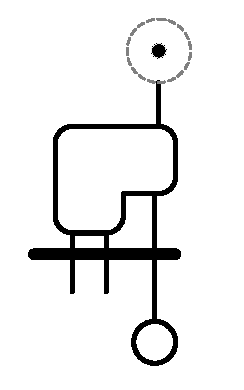
\includegraphics[width=.2\textwidth]{figures/Squiggle.pdf}
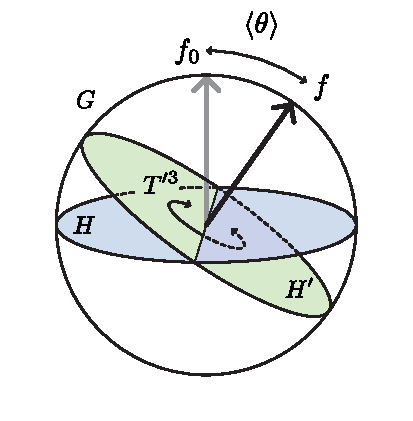
\includegraphics[width=.4\textwidth]{figures/vevtilt.pdf}
\end{center}  


% \vspace{2em}
\vspace*{\fill}

\noindent
\textsf{Last Compiled: \today}

\noindent
\textsf{Image: vacuum misalignment}

\noindent
\textsf{CC BY-NC-SA 4.0}~\ccbyncsa 

\noindent % Course notes URL
% \url{https://github.com/fliptanedo/P231-2023-Math-Methods}

%% Front page logos
\vspace*{\fill}
\begin{center}

\includegraphics[height=.1\textwidth]{figures/FlipAmbigram.png}
\hspace{5em}

\includegraphics[height=.1\textwidth]{figures/UCRPnA_banner.png}
\end{center}

\newpage

\small
\setcounter{tocdepth}{2}
\tableofcontents
\normalsize
\clearpage
\restoregeometry        %% Return to lecture note geometry 
\pagenumbering{arabic}  %% Turn on regular page numbers


%%%%%%%%%%%%%%%%%%%%%
%%%  THE CONTENT  %%%
%%%%%%%%%%%%%%%%%%%%%



%!TEX root = Physics231.tex
\chapter{Introduction}


\section{What is ``Mathematical Methods?''}

This is a \emph{crash course} in the mathematical toolkit necessary for graduate courses in electrodynamics, quantum mechanics, and statistical mechanics. The emphasis is physical intuition rather than mathematical rigor. Let us be clear: as a student you are \emph{expected} to be as mathematically rigorous as your specific discipline requires. Fortunately, there are plenty of excellent textbooks targeted at various levels of rigor and you can find the one most appropriate for you. This course is meant to complement those references, not to replace them.\sidenote{In other words, this is \emph{your} \acro{Ph.D}, craft it appropriately.}

\emph{Unfortunately}, the choice of topics in this course will be neither necessary nor sufficient for your training. If anyone asks, you should say that the theme of this course is to solve the types of linear differential equations that will show up in your physics coursework (\emph{ugh! Boring!}). The actual choice of topics is meant to highlight larger, unifying themes in mathematical physics sprinkled with topics of current research significance.


\section{Green's functions and this course}

Our main goal is to solve linear differential equations:
\begin{align}
  \mathcal O f(x) = s(x) \ .
  \label{eq:greens:function:equation}
\end{align}
In this equation, $\mathcal O$ is a \emph{differential operator}\index{differential operator} that encodes some kind of physical dynamics\footnote{A \textbf{differential operator} is just something built out of derivatives that can act on a function. The differential operator may contain coefficients that depend on the variable that we are differentiating with respect to; for example, $\mathcal O = (d/dx)^2 + 3x\,(d/dx)$.}, $s(x)$ is the \emph{source} of those dynamics, and $f(x)$ is the system's physical \emph{response} that we would like to determine. The solution to this equation is:
\begin{align}
  f(x) &= \mathcal O^{-1} s(x) \ .
\end{align}
This statement is trivial and deeply unsatisfying. We will think carefully about what $\mathcal O^{-1}$ actually means and how to calculate it. $\mathcal O^{-1}$ is the \textbf{Green's function}\index{Green's function} for the differential operator $\mathcal O$. 

\begin{exercise}%
Consider the differential operator $\mathcal O = (d/dx)^2 + 3x\,(d/dx)$. A colleague tells you that $(d/dx)^2$ is squared, therefore it is not a linear operator. Explain why the colleague is mistaken. 
\end{exercise}

To make sense of the object $\mathcal O^{-1}$, we appeal to linear algebra. A linear transformation---that is, a \textbf{matrix}---$A$ acts on a vector $\vec{v}$ to give equations like
\begin{align}
  A \vec{v} = \vec{w} \ ,
\end{align}
whose solution is
\begin{align}
  \vec{v} = A^{-1} \vec{w} \ .
\end{align}
In this course, we think of linear differential operators $\mathcal O$ as infinite-dimensional matrices. $\mathcal O^{-1}$ is the inverse of this matrix. Perhaps you feel a bit nervous because you remember that inverse of a $3\times 3$ matrix is tricky... say nothing of the \emph{infinite} dimensional limit. To assuage this doubt, we remind ourselves that that calculus is infinite-dimensional linear algebra. Complex analysis extends the real line to the complex plane. In so doing, the \emph{analytic structure} of our theories offer both a method to calculate challenging integrals and their own physical significance. 


\section{Two powerful questions}
At any time in this course, you should feel comfortable asking either of the following questions:
\begin{enumerate}
    \item Is it obvious that...?
    \item Why is this significant?
\end{enumerate}
The first question is the way to ask for on-the-spot clarification---I will either appreciate that I did not properly explain a subtle point, \emph{or} I will explain the intuition\sidenote{Your sense of mathematical and physical intuition is incredibly valuable. This is one of the key traits that makes a physics training unique.} for why something should be obvious. The second question is a way to remind me that I may have \emph{lost sight of the forest for the trees}: I want this course to \emph{mathematically connect big ideas in physics}. Asking this question is a reminder that making those connections justifies the hard mathematical work we will put into the course.

\section{Exercises and Examples}
I have tried to insert exercises and examples in these notes. There are still far too few for sound pedagogy. If you really, really want to learn something, you \emph{have} to do exercises. Think of the examples as exercises with solutions---though they are not always written this way. Mull over the exercises: ask yourself why the problems are posed the way they are, challenge the statements to find the domain of validity, think of how one may extend those exercises to other applications. The exercises are a far better gauge of you learning than whether or not you have read a section of the notes. If you are confused reading the text in section 10, it is often the case that you should have been doing the exercises since section 5.

\begin{bigidea}[Do your homework]
Instructors feel no deep satisfaction when you turn in your homework. Instead, an assignment is a pledge to the student to give an opportunity for practice with feedback from someone more experienced.
\end{bigidea}




\section{This is not what I expected}

This is a course in mathematical methods for \emph{physicists}.
%
We do not solve \emph{every} class of differential equation that is likely to pop up in your research careers---that would be a course on mathematical methods for \emph{engineers}\autocite{pirsa_11110040}.\sidenote{I recommend Carl Bender's 2011 lectures at \tacro{PSI} for an insightful course along those lines.} Instead, we methodically dissect a physically motivated example---the harmonic oscillator---to emphasize how we think about mathematical problems. 

We weave together ideas that are not often connected explicitly in undergraduate physics courses: linear algebra, differential equations, complex analysis, statistics. I expect that you have had \emph{some} formal training in these topics so that we may focus on the \emph{interconnections} between these ideas in our study of nature.

Do not be surprised if we only mention Bessel functions in passing. Do not think less of our efforts if we do not calculate Wronksians or go beyond a single Riemann sheet. As graduate students, it is \emph{your} responsibility to be able to grab your favorite reference to apply mathematics as needed to \emph{your} research. \emph{This} course is about the larger narrative that is not often shared explicitly in those books. It is about that which makes physicists employable in Silicon Valley while simultaneously terrible at splitting the bill at a restaurant. 

\begin{example}
Our cavalier attitude towards mathematical rigor should not make you think that mathematical rigor is not necessary. For a nice, visual example, see ``How to lie using visual proofs'' by 3Blue1Brown.\cite{3Blue1Brown_2022}
% https://youtu.be/VYQVlVoWoPY
\end{example}


\section{Nice-ness}
\label{sec:niceness}

I find it useful to invoke the notion of a \textbf{nice}\index{nice} mathematical situation. This is not a formal idea. In fact, it is one of many things that mathematicians find ridiculous about me. However, as a physicist, the concept of mathematical \emph{niceness} is remarkably helpful.

The physical systems that we spend the most time thinking about are all \emph{nice}. 
%
While mathematicians spend years proving every exceptional case to a theorem, we are happy to push onward as long as our mathematical results are true for the \emph{nice} cases. 
%
In fact, nature often admits an \emph{approximately} nice mathematical description.\footnote{This is not because nature is kind, but rather because we are only clever enough to build simple theories. What is important to appreciate as a physicist is \emph{why} simple theories can so nearly approximate nature.}

%
Nice mathematical models make tidy predictions. Then we can Taylor expand about these nice predictions to make better predictions.
%
We sometimes chant \emph{perturbation theory}\index{perturbation theory} out loud several times in case someone watching us does not think we are being rigorous enough.\footnote{Sometimes our Taylor expansions have zero radius of convergence. ``\emph{E pur si muove},'' as Galileo would say. Look up the convergence of the Dyson series.}
% We make Taylor expansions without anguishing about the radius of convergence\footnote{\url{https://johncarlosbaez.wordpress.com/2016/09/21/struggles-with-the-continuum-part-6/}} and validate it post-facto because it \emph{works}.


This is not to say that nature cares at all about our simple physical models. 
%
Every once in a while, we \emph{do} have to worry about the exceptional cases because our models fail to accommodate what is \emph{actually} happening in nature.\footnote{Full disclosure: Your \acro{Ph.D} will likely depend on finding a clever solution to one of these cases.} Those scenarios are the most exciting of all: that is when our mathematical formalism grabs us by the collar and says, \emph{listen to me---something important is happening!} This often happens when a calculation tells us that a physical result is infinite. 

\begin{exercise}\label{ex:hydrogen:problem}
Consider the potential that an electron feels in the hydrogen atom:
\begin{align}
  V(r) &= -\frac{\alpha}{r} \ .
\end{align}
As the electron--proton separation goes to zero, $r\to 0$, the potential goes to infinity. Classical electrodynamics is telling us that something curious is happening. What actually happens? (And why didn't you ask this question when you were in high school?)
\end{exercise}

We focus on \emph{nice} functions and \emph{nice} operators and \emph{nice} boundary conditions, and so forth. We often only need the \emph{nice} math to make progress on our \emph{nice} physical models. It is worth spending our time learning to work with these \emph{nice} limits. Leave the degenerate cases to the mathematicians for now. Eventually, you will find yourself in a situation where physics demands \emph{not nice} mathematics. In that case---and only when the physics demands it---you will be ready to poke and prod at the mathematical curiosity until the underlying \emph{physics} reason for the not-niceness is apparent. All this is to say: if you object to this course because we do not start with proofs about open sets or convergence, then you are missing the point of an education in physics.





\section{Obvious-ness}\label{sec:obviousness}
Finally, I want to comment on the word \emph{obvious}. I write this often. It is somewhat dangerous because it can come off as being arrogant: \emph{this is so obvious to me, if you do not understand you must be deficient}. This is never the reason why I use that word. Instead, the word \emph{obvious} serves a very practical purpose. The goal of this class is not just to be able to ``do stuff'' (e.g.~diagonalize a symmetric matrix), but to also build that intuition that comes from a deeper understanding how the mathematics works. In this sense, every time I write the word \emph{obvious} it is a flag: I am saying something that---with the proper perspective---should be self-evident. If it is not self-evident, then you should stop to interrogate why it is not self-evident. Most likely there is something where a change in perspective may (1) make it obvious, and (2) in so doing deepen your understanding of the subject. So when you see the word `obvious,' I want you to do a quick check to confirm whether or not the statement is indeed obvious. If it is not, then welcome the opportunity to learn.\sidenote[][-3em]{There is, of course, the possibility that what I have written is \emph{not} obvious. For example, if I have made a typo... in which case, please let me know.}

\begin{bigidea}
Speaking of arrogance: physicists sometimes have a reputation for being arrogant. The most generous interpretation is that we must have some Promethean \emph{chutzpah} to seek to comprehend/invent/discover an underlying mathematical organizing principle for the universe. Another manifestation is the damaging ways in which academics can mistreat each other. Somewhere in between are footnotes poking fun at mathematicians, or being a bit of a bore at parties. It is outside the scope of lecture notes on mathematical physics to ask to you to figure out how to be the best version of you-as-physicist-and-human-being that you can realize.\footnote{There are plenty of excellent pieces to reflect on this. For example, \emph{The Disordered Cosmos}, \emph{The Only Woman in the Room}, and \emph{Beamtimes and Lifetimes}.}
\end{bigidea}


\begin{example}
There is a complementary idea that students have a secret superpower that they can exercise. It is terrifying to ask questions in public---after all, what if your peers decide that your question is so basic that you must be \emph{stupid}? There is didactic armor against this. Whenever you are confused, and at the \emph{first appropriate moment} after you are confused, raise your hand and phrase your question as follows:
\begin{quote}
\emph{Is it obvious that} $\ldots$ ?
\end{quote}
Linguistically, this is a trick of the passive voice: it removes \emph{you} from the query. It does not insist that you are incapable of comprehending something, it simply asks if there is some intuitive understanding that you want to make sure you do not miss. After all, developing your physics intuition is one of the goals of your first-year graduate courses. Any self-respecting instructor will respond sympathetically, either:
\begin{itemize}
  \item \emph{no}, it is not obvious. Perhaps then you work through the idea carefully. Or,
  \item \emph{yes}, it is obvious---but only when we remember some previous key step, which your instructor should then highlight.
\end{itemize}
Either way, the result is wisdom rather than risking how you look in front of your peers. 

By the way, \emph{how you look in front of your peers} is not a good reason to do anything. It is almost as bad as not asking questions because you do not want to look stupid in front of your advisor. Here is some free advice: your adviser knows \emph{exactly} how stupid you are. Most likely your advisor does not think you are stupid, but if you are convinced that you are stupid, then rest assured that your advisor knows this and has still chosen to invest their time into you. Make the most of this time: ask questions.
\end{example}

\section{Motivation}

Here are three deeply significant equations in physics:\sidenote{If you want to be fancy, you can add Maxwell's equations. If you want to be \emph{really} fancy, you can write these as $dF=0$ and $-*dF = *J$, but that's for a different course.}\sidenote{We address the $\defeq$ versus $=$ in the next section.}
\begin{align}
    \vec{F} &\defeq m\vec{a}
    \\
    % R_{\mu\nu} - \frac{1}{2}Rg_{\mu\nu} 
    G_{\mu\nu}
    &\defeq \frac{8\pi G_\text{N}}{c^4} T_{\mu\nu}
    \\
    \hat H |\Psi\rangle 
    &= E |\Psi\rangle \ .
    \label{eq:three:equations}
\end{align}
These are Newton's force law, Einstein's field equations, and the Schr\"odinger equation. They govern classical physics, general relativity, and quantum theory, respectively. 


Each equation looks rather unique: they seem to each be speaking their own mathematical language. Newton's law is written with boldfaced vectorial quantities $\vec{F} = (F_x, F_y, F_z)^\trans$ that should look very familiar to any physics undergraduate. Einstein's equation has these funny $\mu$ and $\nu$ indices on every term---have you seen these before? Do they look intimidating? If you ever want to make your equations look ``technical'' and ``physicsy,'' you should dress them up with indices. The Schr\"odinger equation has no indices, but instead has these funny angle-brackety things... and that $\hat H$ looks suspicious. Where did $H$ get a hat, and what is the content of this equation other than $\hat H = E$?

\emph{Each of these equations turns out to be a ``vectorial'' equation.} Each one is actually shorthand for a number of equations. Newton's equation is shorthand for three equations, one for each component. Einstein's equation is shorthand for 16 equations, one for each combination of the indices $\mu$ and $\nu$ that run over four values\sidenote{The four values are the three directions of space and one direction of time.}. The Schr\"odinger equation is shorthand for an \emph{infinite} number of equations, one for each allowed energy of a quantum system.

The mathematical formalism that unifies these different ideas (and notations) of `vector' is called linear algebra. It may sound humble: after all, ``linear'' systems are \emph{easy}, aren't they? Did we not just spend years of our lives learning fancy things like \emph{calculus} and \emph{differential equations} to deal with functions that are more complicated than \emph{lines}? In some sense, yes: linear algebra is about lines and planes in different numbers of dimensions.\sidenote{On the other hand: a good chunk of the calculus that we do is also implicitly linear. Physicists often Taylor expand and keep only the $\mathcal O(\varepsilon)$ term. Integration boils down to summing trapezoids whose angley-bits are given by the first derivative of a function... the linear component.} However, linear algebra turns out to be far more richer than what you may be used to from high school. 

In this course we will see how the three equations in \eqref{eq:three:equations} are connected by the mathematics of linear algebra. We will dive into the different notation and shamelessly pass between $\vec{v}$, $v^i$, and $\ket{v}$ to describe the same abstract vector. We will connect to the mathematical description of \emph{symmetry} and see how it is an underlying theme in our descriptions of nature. And we will do all of this in a way that will make the instructors of the linear-algebra-for-mathematicians course and linear-algebra-for-engineers course vomit a little in disgust. Consider that one of privileges of being a physicist.

\section{Equality}

You may have noticed in \eqref{eq:three:equations} a distinction between two different equal signs: the standard equality $=$ and the definition, $\defeq$. Physicists often write both of theses as $=$, even though conceptually they mean hugely different things\autocite{2019per8.conf..471A,Alaee_2022}. I adopt the following notation:
\begin{itemize}
  \item The equal sign $=$ means two sides of an equation evaluate to the same quantity. This is the equal sign you use when simplifying an expression by applying mathematical identities. For example, $\D{x^2}/\D{x} = 2x$.
  \item The definition $\defeq$ means the left-hand side is \emph{defined} to be the right-hand side. My idiosyncratic notation is inspired by \emph{Mathematica}. When writing by hand I use $\stackrel{\cdot}{=}$. Other sources may use a triple bar (used below). For example, $\dot{x}\defeq \D{x}/\D{t}$.
  \item I reserve the triple equal sign $\equiv$ for `tautologically equivalent.' I do not have a rigorous definition for this, but the idea is rather useful as a shorthand for the word ``obvious,'' see Section~\ref{sec:obviousness}.\sidenote{I think I picked up this notation early in my university education during a lecture by Yakov Eliashberg in 2002. I have a clear memory of him responding to a question about an equal sign by impishly smiling and saying that the equality is tautological, then saying that perhaps writing an extra bar on the equal sign would make it more clear. At the time we, the students, found this completely vexing---but we came to quickly appreciate its utility. Other variants of this from Eliashberg did not stick, like a `triple-$u$' variable as the third in a sequence after $u$ and double-$u$.} It means ``this is so true that there is nothing I can write to justify it---if you are confused, you may want to take a step back to see if there is a different way of looking at the idea.'' For example, mint chocolate chip ice cream $\equiv$ the best.
\end{itemize}
There are two other binary relations worth noting. The first is $\approx$, a statement that two sides are \emph{almost} equal (``almost =''). This is like a `lower class' version of the equal sign. Perhaps amusingly, there is also $\sim$, which I argue is \emph{more} important than the equal sign. It is so significant that we dedicate an entire paragraph to it in Section~\ref{sec:sim:binary:relation}.

\section{One last piece of advice}

It took me way too long to appreciate the crucial significance of homework and exercises in learning physics. Your job in your \acro{Ph.D} is to answer questions where no previous answer had ever existed in the history of humanity. You will be guided by your advisor and your mentors, but you will be the discover-er of new truth. This is a tall order, something like completing a marathon or climbing Everest. And like those physical feats, the only way to succeed in your intellectual pursuit is to \emph{practice}\sidenote{I encourage you to look up Allen Iverson's 2002 ``Practice'' press conference and the vertbatim homage in \emph{Ted Lasso} Season 1 Episode 6.}. And the best training we have in physics are practice problems. These are problems that are crafted to hone your skills. They are examples that are assured to be \emph{solvable}\sidenote{The fact that they are solvable does not mean that you are entitled to a solution set other than the solution that you earn by deriving it yourself.} and with a framework (like a course with peers) to guide you through the challenges. Do not squander the opportunity to \emph{train}. My undergraduate advisor used to say, \emph{you should do every problem in the book---but especially the ones that you cannot do.}

\chapter{Dimensions}\label{ch:dimensions}


\flip{To add: \url{https://youtu.be/kkfIXUjkYqE}}

You may be surprised how far one can go in physics by thinking deeply about dimensional analysis. Here we only get started. To take the next step, you may read more about the Buckingham Pi theorem or applications in physics. I recommend any of the following references: \autocite{doi:10.1119/1.1987069, doi:10.1119/1.4902882, doi:10.1119/1.3535586, Stevenson:1980ga}.
\textbf{Dimensional analysis}\index{dimensional analysis} is simply the idea that by keeping track of the units of physical quantities, we can learn quite a bit about how those quantities must show up in our physical laws.


\section{Physics versus Mathematics} 

Let us make one point clear:
\begin{align}
  \text{Physics} \neq \text{Mathematics} \ .
\end{align}
This is a truth in many different respects. The astronomer Fritz Zwicky (Fig.~\ref{fig:zwicky}) might have called this a \emph{spherical truth}: no matter how you look at it, the statement is still true.\sidenote{Zwicky has such an oft-repeated reputation for having a challenging personality that his daughter has argued and litigated that scientists have deliberately colluded to use this reputation to minimize Zwicky's legacy---see ``The Father of Dark Matter Still Gets No Respect'' by Richard Panek in \emph{Discover}, 30 Dec 2008. I suspect it does not help when one's most enduring photo is the one in Fig.~\ref{fig:zwicky}.}:
\begin{marginfigure}%[th]
    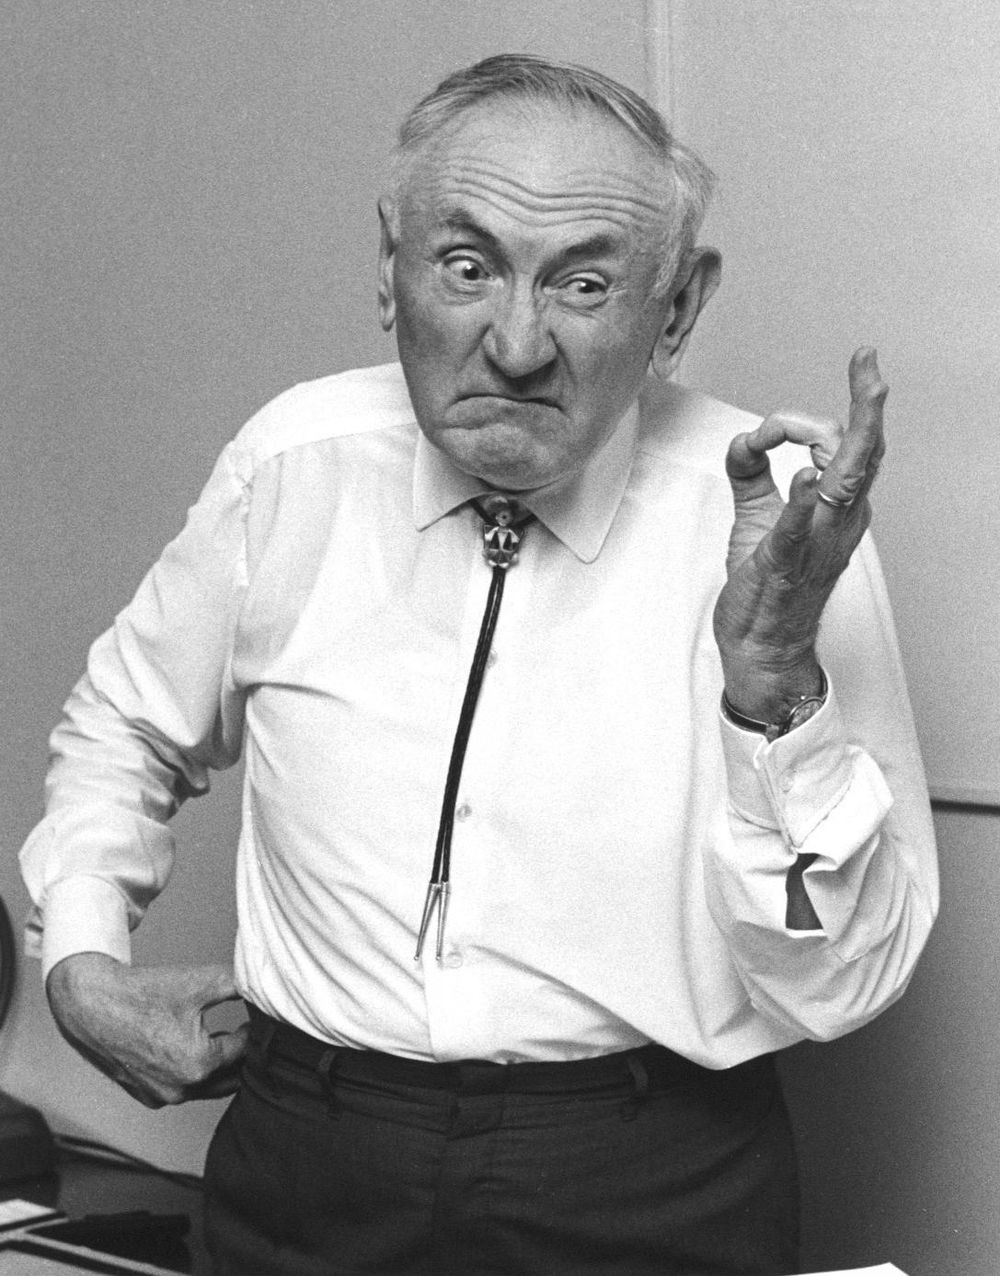
\includegraphics[width=.8\textwidth]{figures/zwicky_caltecharchives.jpg}
    \captionsetup{font={scriptsize,sf}}
    \caption{The photo of Zwicky that often appears in public talks about dark matter. From the Caltech archives (1971, identifier 10.12-64).}
    \label{fig:zwicky}
\end{marginfigure}
\begin{itemize}
  \item Physicists are rooted in experimental results. {Even theorists? \emph{Especially} theorists.}
  
  \item Physicists Taylor expand to their hearts’ content. Even when it is sometimes not mathematically valid.~\autocite{Baez_Azimuth_2016}

  \item Physicists pick a basis, use coordinates, and decorate every tensor with indices. {Equations in physics appear intimidating because of the indices decorating our variables. Ironically, physicists are often intimidated by mathematics because of the conspicuous absence of any indices.}.

  \item Physicists seek truths about \emph{this} universe.

  \item Physicists have a fast and loose relationship to the concept of infinity and the related concept of the infinitesimal---on this, I recommend Jim Holt's essay ``The Dangerous Idea of the Infinitesimal.''~\autocite{holt2018einstein}
  At the same time, many of our tools seem to \emph{beg} questions about the infinite.
\end{itemize}
My friends, we are not doing mathematics. 

\subsection{The most important binary relation}
\label{sec:sim:binary:relation}

When we write equations, the symbol that separates the left-hand side from the right-hand side is a binary relation. We use binary relations like $=$ or $\neq$. Sometimes to make a point we write $\cong$ or $\equiv$ or $\dot =$ to mean something like `definition’ or `tautologically equivalent to’ or some other variant of \emph{even more equal than equal}. 

 \begin{figure}[h]
      \caption{Mathematical symbol fight from \tacro{XKCD}.~\cite{xkcd_2343} \tacro{CC BY-NC 2.5} \label{fig:xkcd:symbol}} 
      % \includegraphics[width=\textwidth]{mathematical_symbol_fight_2x.png} % or tikz or anything
      \includegraphics[width=\textwidth]{figures/mathematical_symbol_fight_2x.png}
  \end{figure}
% xkcd_2343

As physicists the most important binary relation is none of those things\sidenote{I thank Yuval Grossman teaching me this.}. What we usually care about is  $\sim$.\sidenote{I use this the same way as $\propto$, which is completely different from `approximately,’ $\approx$.} The symbol $\sim$ tells us how how something \emph{scales}. If I double a quantity on the right-hand side, how does the quantity on the left-hand side scale? Does it depend linearly? Quadratically? Non-linearly? The answer encodes something important about the underlying physics of the system. The symbol $\sim$ the reason why \emph{imagine the cow is a sphere} is a popular punchline in a joke about physicists. 


Implicit in this discussion is the pragmatic policy that we will not care about stray factors of 2 in this class. As my adviser used to say, if you are worried about a factor of 2, then you have addition homework to figure out that factor of 2.\sidenote{That being said, you are reading these notes and find an error, do let me know about it.} 

\subsection{Units}

There is another way in which physics is different from mathematics. It is far more prosaic. \emph{Quantities in physics have units}. We do deal in simply numbers, we deal with kilograms, electron volts, meters. It turns out that dimensional analysis is a big part of what we do as physicists. 

\begin{exercise}\label{ex:trancendental}
Explain, in words, why the quantity $\sin(3~\text{cm})$ is absolute nonsense in any context. What about $\text{exp}(2~\text{kg})$?
\end{exercise}

\begin{example}
Did you use a Taylor expansion in your solution to Exercise~\ref{ex:trancendental}? That type of argument is something like this:
\begin{align}
\e^{2~\text{kg}} = 1 + (2~\text{kg}) + \frac{1}{2!}(2~\text{kg})^2 + \cdots \ ,    
\end{align}
from which we see that each term has different powers of mass. Did you catch where I lied to you? Recall that Taylor expansions are of the form
\begin{align}
    f(x+\Delta x) 
    = f(x) + \frac{ \D{f}(x) }{ \D{x} } \Delta x + 
    \frac{1}{2!} \frac{ \D[2]{f}(x) }{ \D{x}^2 } \Delta x^2 + \cdots \ .
\end{align}
Clearly each term has the same dimension because the units in $\Delta x$ cancel those of $\D{x}$. In fact, the underlying reason why trancendental functions cannot take dimensionful arguments is simply that they have no meaningful definition.\autocite{doi:10.1021/ed1000476} 
\end{example}

\section{Converting Units}

Imagine that you have three apples. This is a number (three) and a unit (apple). The meaning of the unit depends on what you're using it to measure. For example, if apples are \$1 each, then you could use an apple as a unit of currency. The way to do this is to simply \emph{multiply by one}:
\begin{align}
  (3\text{ apples}) \times \left(\frac{\text{\$ 1}}{\text{apple}}\right)
  &= \$ 3 \ .
\end{align}
We have used the fact that the exchange rate is simply the statement that
\begin{align}
  1\text{ apple} &= \$1
  & \Rightarrow &&
  1 &= \frac{\$ 1}{1\text{ apple}} \ .
\end{align}
You can do a similar thing for [kilo-]calories or any other conversion rate. 

All that matters is that the conversion factor is a constant. The constants of nature make very good `exchange rates.' For example, high-energy physicists use \textbf{natural units}\index{natural units}:
\begin{align}
  \hbar = c = 1 \ .
\end{align}
At face value, this does not make sense. $\hbar$ has units of action, $c$ is a speed, and 1 is dimensionless. In more conventional units,\sidenote{For the most part, we are happy with one significant figure in this course.}
\begin{align}
  c &= 3 \times 10^{10}~\text{cm}/\text{s} 
  &
  \hbar &= 10^{-34}~\text{kg}~\text{m}^2/s
  \ .
\end{align}
However, because nature gives us a \emph{fundamental} unit of action and a \emph{fundamental} unit of speed, we may use them as conversion factors (exchange rates). If $c=1$, then 
\begin{align}
  1~\text{s} &=  3 \times 10^{10}~\text{cm} \ .
\end{align}
This connects a unit of time to a unit of distance. By measuring time, the constant $c$ automatically gives an associated distance. The physical relevance of the distance is tied to the nature of the fundamental constant: one second (or `light-second') is the distance that a photon travels in one second. Observe that this only works because $c$ is a constant. 

\section{Quantifying units}

We use the notation that a physical quantity $Q$ has \textbf{dimension}\index{dimension} $[Q]$ that can be expressed in terms of units of length, mass, and time:
\begin{align}
  [Q] = L^a M^b T^c \ .
\end{align}
The {dimension} is the statement of the powers $a$, $b$, and $c$. You may want to also include units of, say, electric charge. Sticklers may pontificate about whether electric charge formally carries a new unit or not. 

\begin{example}
What are the units of force? We remember that $\vec{F} = m\vec{a}$, so 
\begin{align}
  [\vec F] &= [m][\vec{a}] = M\times L T^{-2} = L^1 M^1 T^{-2} \ .
  \label{eq:02:force:units}
\end{align}
\end{example}

\begin{exercise}
What are the units of the fine structure constant?
\end{exercise}

When working in \textbf{natural units}, $c=1$ means that units of length and time are the same and $\hbar = 1$ means that units of time and energy (mass) are inversely related. In natural units, one simply writes $[Q]$ to mean the mass-dimension of a quantity. To revert back to conventional units, one simply multiplies by appropriate factors of $1=c$ and $1=\hbar$. 

\begin{example}
What are the units of force in natural units? From \eqref{eq:02:force:units} we multiply by one to convert length and time into mass dimensions:
\begin{align}
  [\vec F] &= [c^{-3} \hbar \vec{F}] = M^2 \ .
\end{align}
In natural units we say $[\vec F] = 2$. Recall that energy and mass have the same dimension, which you may recall from the Einstein relation $E^2 = m^2c^4 + p^2c^2$.
\end{example}

\section{Dimensional analysis at work}

\subsection{Sanity Check}

The simplest use of dimensional analysis is to check your work. The following expression is obviously wrong:
\begin{align}
  1 + (3~\text{cm}) \ .
\end{align}
This does not make sense. You cannot sum terms with different dimensions. Similarly, $\sin(3\text{ cm})$ does not make sense. What about $e^{5~\text{cm}}$? This doesn't make sense because
\begin{align}
  e^x = 1 + x + \frac{1}{2!} x^2 +  \cdots
\end{align}
Since each term comes with a different power of $x$, the argument of the exponential must be dimensionless. 

\begin{example}
As pointed out by Matta et al.\footnote{\emph{J.~Chem.~Educ.} 2011, 88, 1, 67–70. \url{https://doi.org/10.1021/ed1000476}}, this argument is not quite correct. Each term in the Taylor expansion of a function $f(x)$ maintains the dimensions of $f(x)$, as is obvious when written out carefully:
\begin{align}
  f(x_0+\Delta x) = f(x_0) + \left.\frac{df}{dx}\right|_{x_0}\Delta x + \frac{1}{2}\left.\frac{d^2f}{dx^2}\right|_{x_0}\Delta x^2 + \cdots \ .
\end{align}
The units of every $dx^2$ in the `denominator' of $d^{(n)}f/dx^n$ is canceled by the units in $\Delta x^n$, no matter what the dimensions of $\Delta x$ are.
%
The real issue is that for many functions, $f(x_0)$ is simply not defined for dimensionful arguments. This is certainly true for trigonometric functions. For the exponential, one may fall back to the limit definition:
\begin{align}
  e^x = \lim_{n\to\infty} \left(1+ \frac{x}{n}\right)^n \ ,
\end{align}
where it is now an issue of different terms having different dimensions. Note that the right-hand side is not a Taylor expansion. The exponential definition above is handy because it makes sense even when $x$ is a matrix or operator.
\end{example}

\begin{exercise}
Sometimes you may think it is useful to keep track of radians (or degrees) as a dimensionful quantity. This, by the way, is a slippery slope because then you may want to think of $\pi$ as some unit of circles... whatever that means. Following the exercise above, show that (1) each term in the Taylor expansion of $f(x) = \sin(x)$ has the same dimensions, and (2) that there is no issue with trigonometric functions being defined as having `dimensionful' arguments in this way.
\end{exercise}

\begin{exercise}
Consider the energy spectrum of light emitted from some constant source---a distant star, the ongoing annihilation of dark matter in the galactic center, or a high-intensity laser. The spectrum encodes how many photons are emitted per unit time. We can plot this spectrum as a curve on a graph. We can even normalize the curve so that it integrates to one photon. This means we only care about the distribution of energy, not the absolute amount. The horizontal axis of such a plot is the photon energy. What are the units of the vertical axis?
\end{exercise}

\subsection{Solving problems}

Here is a common problem in introductory physics. Assume you have a pendulum with some sufficiently small initial displacement $\theta_0$. What’s the period, $\tau$ of the pendulum? We draw a picture like Fig~\ref{fig:simple_pendulum}.
%
% \marginfig{figures/lec01_pendulum.pdf}{Sketch of a simple pendulum.}{fig:simple_pendulum}
\begin{figure}[tb]
    \centering
    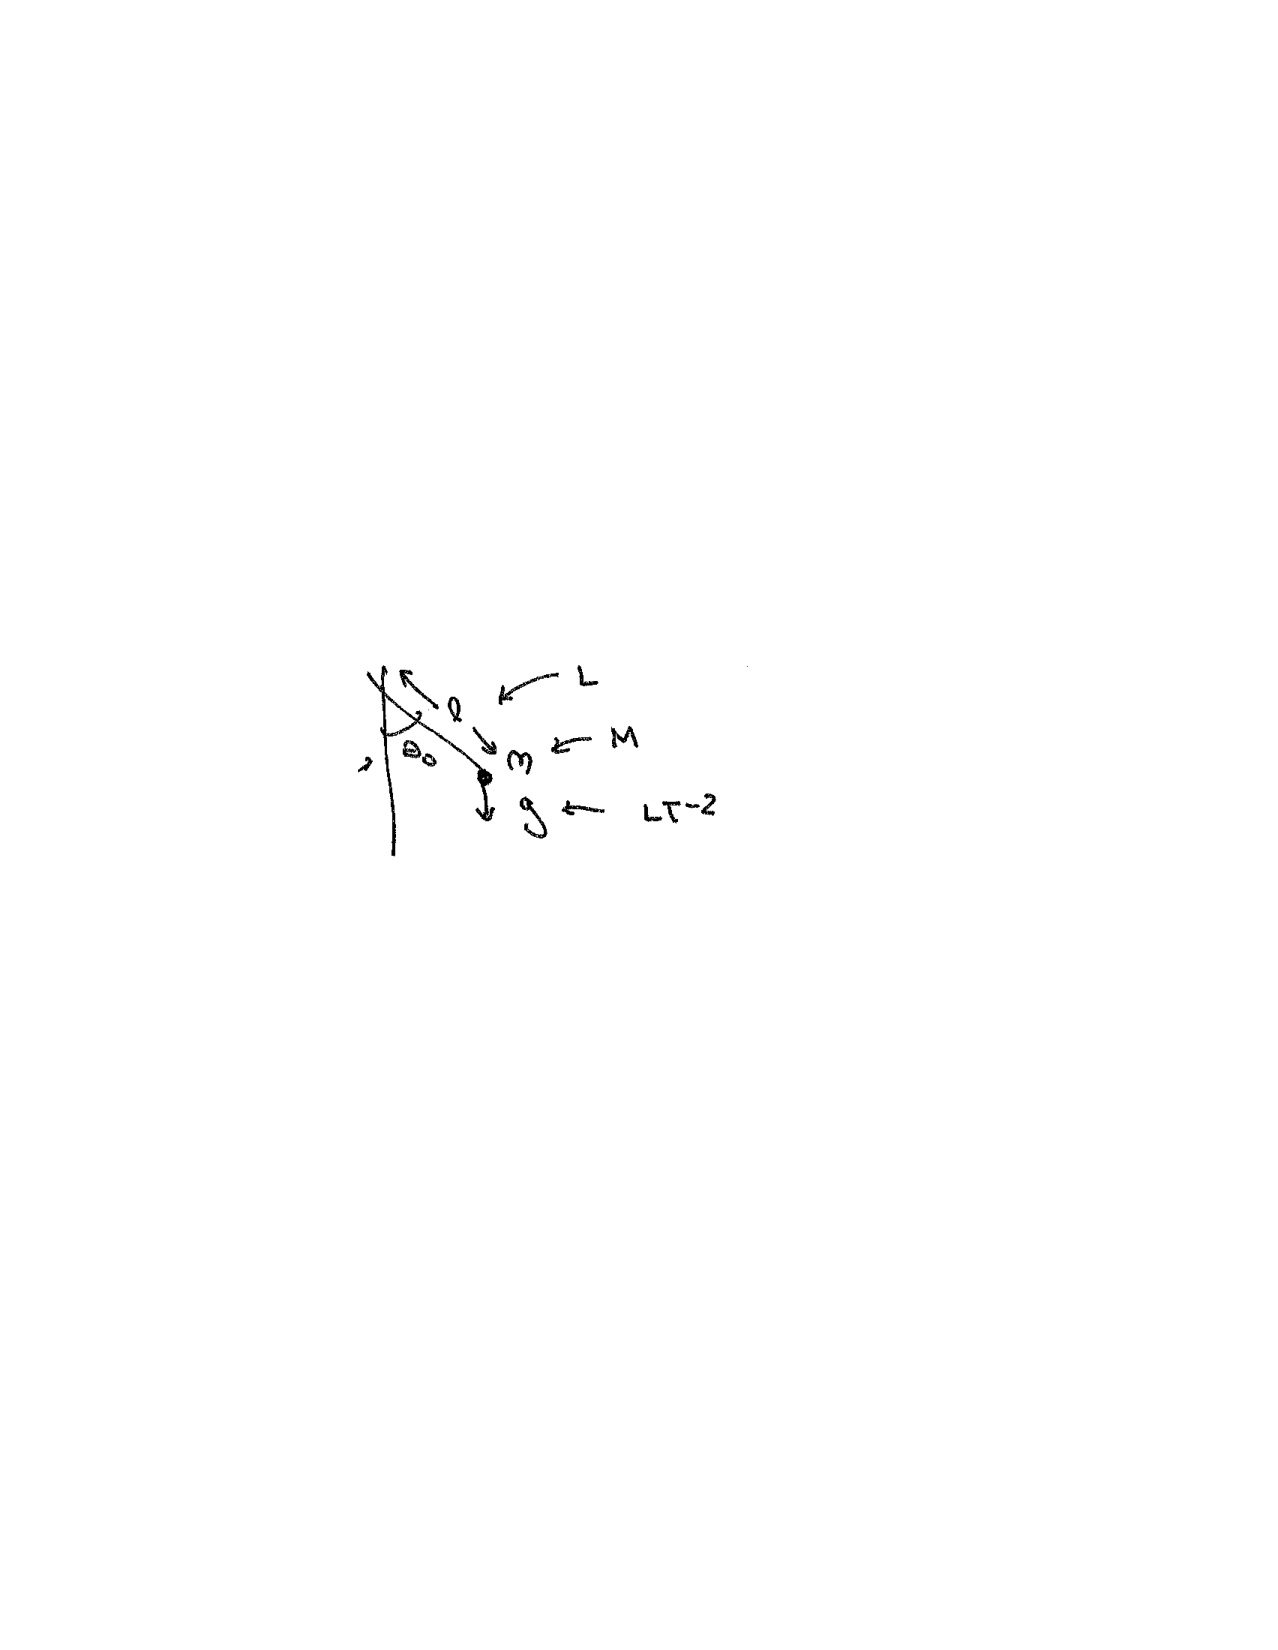
\includegraphics[width=.5\textwidth]{figures/lec01_pendulum.pdf}
    \caption{Sketch of a simple pendulum.}
    \label{fig:simple_pendulum}
\end{figure}
%
%
From dimensional analysis, we know that the period has dimensions of time, $[\tau] = T$. The problem gives us a length $[\ell]=L$ and the gravitational acceleration, $[g]=LT^{-2}$. Note that $[\theta_0] = 1$ is dimensionless. This means that the only way to form a quantity with dimensions of time is to use $g^{-1/2}$. This leaves us with a leftover $L^{-1/2}$, which we can fix by inserting a square root of $\ell$:
\begin{align}
  \tau \sim g^{-1/2} \ell^{1/2} \ .
\end{align}
If we want to be fancy, we can make this an equal sign by writing a function of the other dimensionless quantities in the problem:
\begin{align}
  \tau = f(\theta_0) \sqrt{\frac{\ell}{g}} \ .
\end{align}

\flip{To do:include problems from R.W.~Robinett \emph{American Journal of Physics} \textbf{83}, 353 (2015); \url{https://doi.org/10.1119/1.4902882}.}


\begin{example}
In an introductory physics class, one finds that $f(\theta_0)\approx 2\pi$ in the small angle approximation, $\sin\theta \approx \theta$. Thus the leading order result is independent of the initial angular displacement---a fact that appears \emph{almost} as remarkable as the independence from mass when we first learn this.
\end{example}

\begin{example}
There is a historical consequence of the small angle formula, $\tau = 2\pi \sqrt{\ell/g}$: in meter--kilogram--seconds units, $g \approx \pi^2$~meters per second$^2$. Huygens' early definition for the meter was that a pendulum should complete one full oscillation in two seconds. We find that $g = \ell(2\pi/\tau)^2$. Plugging in $\tau = 2$~seconds and $\ell = 1$~meter gives the approximate relation. The relation is merely approximate due to later redefinitions of the meter.\footnote{Grigory Zaytsev, \url{https://roitman.io/blog/91}}
\end{example}

\subsection{Scaling}

A key theme in physics is scaling relations. We present a somewhat contrived example of how this works adapted from section 11 of V.\ I.\ Arnold's \emph{Mathematical Methods of Classical Mechanics}.\sidenote{This is one of my favorite differential geometry textbooks because it is disguised as a book on mechanics.}. Suppose you have some static, central potential $U(\vec r)$. Maybe it is some planet orbiting a star. 
%
% \textfig[1]{figures/lec01_orbit.pdf}{A orbital trajectory, $\vec{r}_0(t)$.}{fig:simple_orbit}
\begin{figure}[tb]
    \centering
    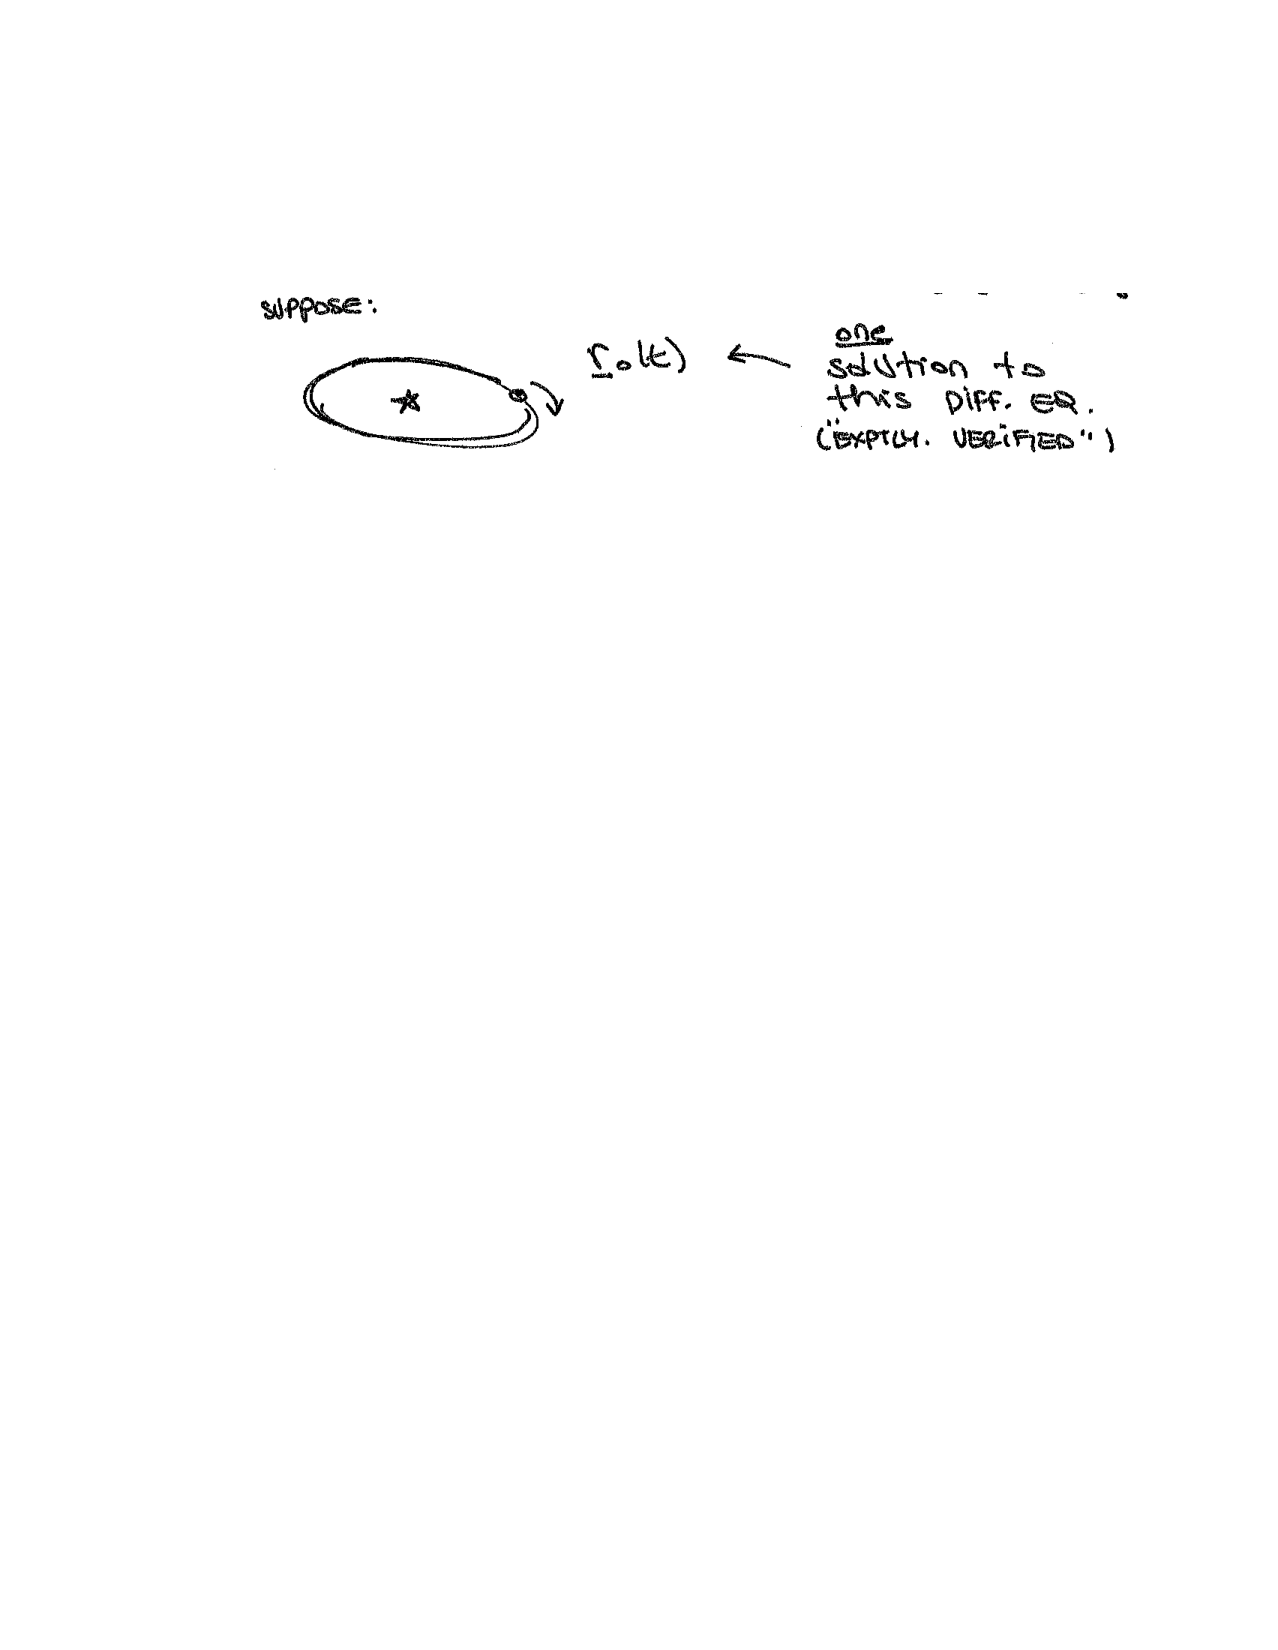
\includegraphics[width=.5\textwidth]{figures/lec01_orbit.pdf}
    \caption{A orbital trajectory, $\vec{r}_0(t)$.}
    \label{fig:simple_orbit}
\end{figure}
%
The force law gives:
\begin{align}
  m 
  \ddot{\vec{r}} = - \frac{\partial U}{\partial\vec{r}} \ .
  \label{eq:scaling:eg}
\end{align}
Suppose we are given a solution, $\vec r_0(t)$. Perhaps this is a trajectory that is experimentally verified. Dimensional analysis gives us a way to scale this solution into other solutions. For example, let us scale time by defining a new variable $t'$:
\begin{align}
  t \equiv \alpha t' \ .
\end{align}
Because the potential is static, then only the left-hand side of the force law changes. Even though the right-hand side formally has dimensions of time, $T^{-2}$, it does not transform because those units are carried in a constant, perhaps $G_N$, not a $(d/dt)^2$ like the left-hand side. The left-hand side of the force law gives:
\begin{align}
  m\left(\frac{d}{dt}\right)^2 \vec r_0(t) 
  &=
  m\alpha^{-2} \left(\frac{d}{dt'}\right)^2 \vec r_0(\alpha t') \ .
\end{align}
This begs us to define a new mass $m' = m\alpha^{-2}$ so that
\begin{align}
   m' \left(\frac{d}{dt'}\right)^2 {\vec{r}_0}(\alpha t')
  = - \frac{\partial U}{\partial\vec{r}_0} \ .
\end{align}
What this tells us is that we may define a new trajectory, $\vec r_1(t') \equiv \vec{r}_0(\alpha t')$, which is a solution in the same potential that traces the same trajectory but at $\alpha$ times the speed and with mass $m'$. Changing labels $t'\to t$ for a direct comparison:
\begin{align}
   m' \left(\frac{d}{dt}\right)^2 {\vec{r}_1}(t)
  = - \frac{\partial U}{\partial\vec{r}_1} \ ,
\end{align}
which is indeed\sidenote{We were able to swap $\vec r_0$ with $\vec r_1$ simply because $U$ only depends on the position.} \eqref{eq:scaling:eg} with a new mass $m'$ and a trajectory $\vec r_1(t') \equiv \vec{r}_0(\alpha t')$. For example, if $\alpha = 2$, then $\vec r_1(t)$ traces the same trajectory at double the velocity with one fourth of the mass.

\begin{exercise} 
I missed something in the example above. In order for a planet of mass $m'$ to have trajectory $\vec r_1(t')$, what is the mass of the star compared to the original mass $M_\star$?\footnote{Thanks to Eric Zhang (2021) for pointing this out.} 
\end{exercise}

\begin{example} 
Business-y people like to quantify effort using words like `person--hour' or `person--years.' This is the idea that a 10 person--hour task would take 10 people one hour to complete, or one person 10 hours to complete, or 5 people two hours to complete, etc.  As you can see, this choice of units implies that effort has a linear scaling in both the number of people and the amount of time needed. Anyone who has worked on a group project knows that this linear scaling is bullshit. Frederick Brooks reflects on this in the 1974 essay, ``Myth of the Man--Month.''\autocite{Brooks1975}
\end{example}

\subsection{Error Estimates}

This section is based on a lovely \emph{American Journal of Physics} article by Craig Bohren.~\autocite{doi:10.1119/1.1574042}%\footnote{\url{https://doi.org/10.1119/1.1574042}} 
Let us go back to another high school physics problem: we drop a ball of mass $m$ from height $h$. See Fig.~\ref{fig:simple_drop}. The task is to find the time $t_0$ for the ball to hit the ground.
%
% \marginfig{figures/lec01_drop.pdf}{Dropping a ball of mass $m$.}{fig:simple_drop}
\begin{figure}[tb]
    \centering
    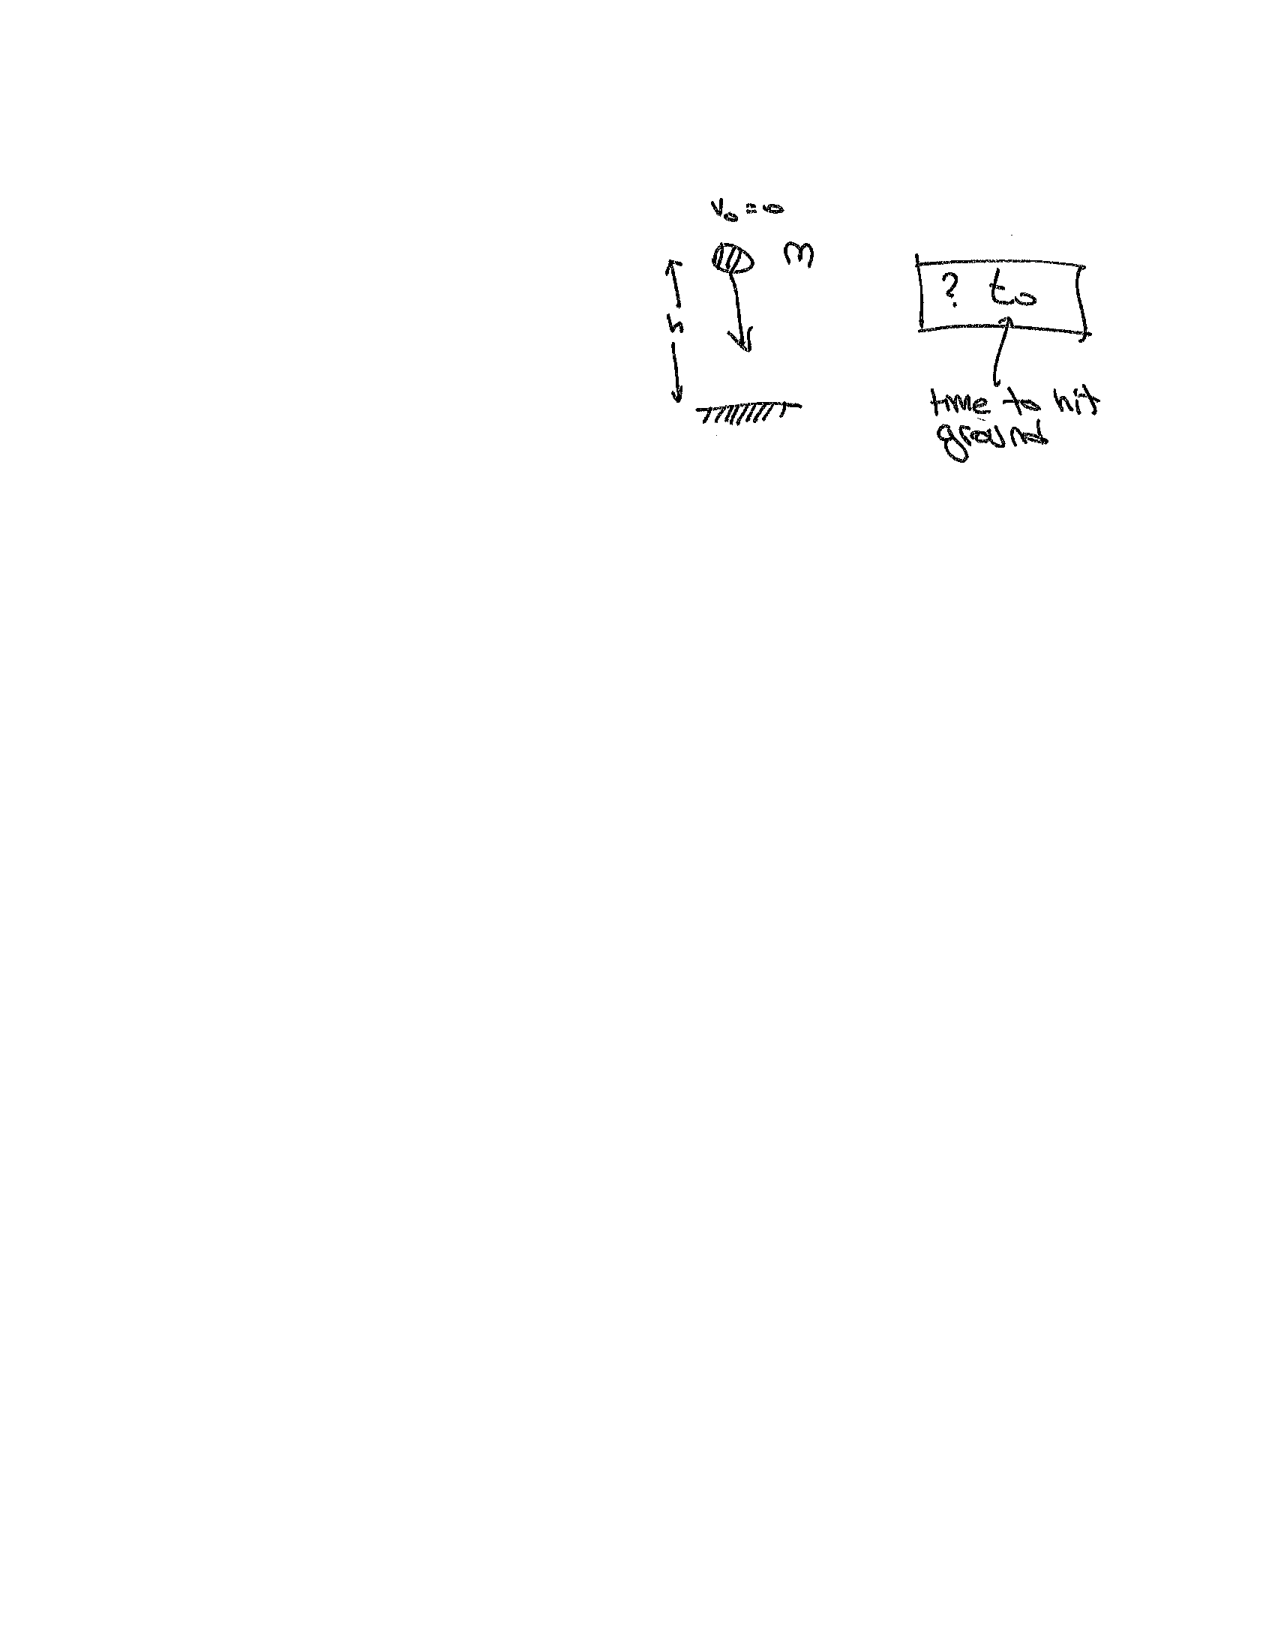
\includegraphics[width=.5\textwidth]{figures/lec01_drop.pdf}
    \caption{Dropping a ball of mass $m$.}
    \label{fig:simple_drop}
\end{figure}

% Suppose you drop a mass $m$ from height $h$ that is initially at rest. How long before this hits the ground? 
You can integrate the force equation to get
\begin{align}
  t_0 = \sqrt{\frac{2h}{g}} \ .
\end{align}
This is the \emph{exact} answer \emph{within our model} of the system. The model made several assumptions: the mass is a point mass, the gravitational acceleration is constant at all positions, there is no air resistance, etc. In fact, we \emph{know} that if we do an experiment, our result will almost certainly \emph{not} be $t_0$. All we know is that $t_0$ is probably a good approximation of the actual answer. What we would like to to know is: \emph{how good of an approximation is it?}

One way to check this is to do the next-to-leading order (\acro{NLO}) calculation, taking into account a more realistic model and then compare to $t_0$. Of course, ``more realistic'' is also code for ``more complicated.'' Take a moment to appreciate that doing this is \emph{stupid}. Why do we need to do a \emph{hard} calculation to justify doing an \emph{easy} one? If we are going to do the hard calculation anyway, what was the point of ever doing the easy one?

What we really want is an error \emph{estimate}. The error\index{error} is
\begin{align}
  \epsilon &= \frac{t_1 - t_0}{t_0} \ .
\end{align}
This is a dimensionless quantity that determines how far off $t_0$ is from a more realistic calculation, $t_1$. Ideally we should not actually have to do much work to estimate $t_1$. 

Let us assume that we are not completely nuts and that we are in a regime where the error is small\sidenote{Note the error has to be dimensionless in order for us to be able to call it `small,` otherwise it begs the question of `small with respect to what?'}. Then the error is a function of some dimensionless parameters, $\xi$, in the system. We define these $\xi$ so that as $\xi \to 0$, $\epsilon(\xi) \to 0$. In other words, the approximation gets better as the $\xi$ are made smaller. By Taylor expansion:
\begin{align}
  \epsilon(\xi) = \epsilon(0) + \epsilon'(0) \xi + \mathcal O(\xi^2) \ .
\end{align}
By assumption, $\epsilon(0) = 0$ and $\mathcal O(\xi^2)$ is  small. We can then make a reasonable \emph{assumption} that the dimensionless value $\epsilon'(0)$  is $\mathcal O(1)$. This tells us that the error goes like $\epsilon(\xi) \sim \xi$.

By the way $\mathcal O(1)$ is read ``order one'' and is fancy notation for the order of magnitude. Numbers like 0.6, 2, and $\pi$ are all $\mathcal O(1)$. A number like $4\pi$, on the other hand, is $\mathcal O(10)$.  The assumption that a dimensionless number is $\mathcal O(1)$ is reasonable. When nature gives you a dimensionless parameter that is both (a) important and (b) very different from $\mathcal O(1)$, then there's a good chance that it's trying to tell you something about your model. Good examples of this are the cosmological constant, the strong \acro{CP} phase, and the electroweak hierarchy problem.\sidenote{There are also `bad' examples. The ratio of the angular size of the moon to the angular size of the sun is unity to very good approximation. This is quite certainly a coincidence. Our universe appears to be in an epoch where the density of matter, radiation, and dark energy all happen to be in the same ballpark. Our cosmological models imply that this is purely a coincidence. It would be very curious if this were not the case. As an exercise, you can critically explore the use of the anthropic principle in physics.} 

Here is how it works in practice. One effect that we miss in our toy calculation of $t_0$ is that the earth is round with radius $R$. This means that assuming a constant $g$ is an approximation. We have two choices for a dimensionless parameter $\xi$:
\begin{align}
  \xi &= \frac{h}{R}
  &\text{or}&&
  \xi &= \frac{R}{h} \ .
\end{align}
There is an obvious choice: $\xi = h/R$, because we know that as $h$ is made smaller (drop the ball closer to the ground) or $R$ becomes bigger (larger radius of Earth) then the constant $g$ approximation gets better. We thus expect that the corrections from the position-dependence of $g$ go like $\mathcal O(h/R)$.
 
% Exercise: check by explicit calculation, 2017 lec 1
\begin{exercise}
    Check by explicit calculation that the correction to the constant $g$ approximation is linear in $h/R$. Start by writing the force law for a point source of at distance $r=R+h$ from the center of the Earth. Taylor expand to find a second order differential equation that is difficult to solve:
    \begin{align} 
      \ddot{h} = \frac{-g}{\left(1+\frac{h}{R}\right)^2} \ .
    \end{align}
    Taylor expand to reduce this to an equation of the form
    \begin{align}
      \frac{d^2 q}{ds^2} = -1 + 2q \ ,
    \end{align}
    Here we define the natural dimensionless variables, $q = h/R$ and $s = \left(g/R\right)^{1/2} t$. If the choice of $s$ is not obvious, please do everything in terms of $t$ and then observe that one can conveniently absorb a factor of $g/R$ into dimensionless time variables.\footnote{You should find an equation of the form $\ddot q = -(g/R)(1-\cdots)$.} Plug the dimensionless differential equation into \emph{Mathematica} or your favorite symbolic solver to obtain 
    \begin{align}
      q(s) = c_1 e^{\sqrt{2}s} + c_2 e^{-\sqrt{2} s} + \frac{1}{2} \ .
    \end{align}
    Argue that the initial condition $\left.\dot h(t)\right|_{t=2} = 0$ implies that the coefficients satisfy $c_1 = c_2$ so that you can combine the exponentials into a hyperbolic cosine. 
    % If $q_0$ is the value of $q(s)$ at $t=0$, show that $c_1 = (q_0  - 1/2)/2$.
    Show that one obtains:
    \begin{align}
      \frac{2q(s) - 1}{2q(0) -1} = \cosh(\sqrt{2}s) \ .
    \end{align}
    Argue why you can Taylor expand the right-hand side about small argument; that is, explain why $s \ll 1$. (Hint: use $h\ll R$.) Perform the Taylor expansion of the hyperbolic cosine to find that the leading correction to the fall time is
    % 
    \begin{align}
      s_1 = \frac{2q_0}{1-2q_0} \ .
    \end{align}
    % 
    The zeroth order approximation was $s_0 = (g/R)^{1/2} t_0 = \sqrt{2q_0}$. Calculate $(s_1 - s_0)/s_0$ to confirm that this is $\mathcal O(h/R)$. 
\end{exercise}

\subsection{Bonus: Allometry}

There is a fun topic called \textbf{allometry}.\index{allometry} This is basically dimensional analysis applied to biology. A typical example is to consider two people who have roughly the same shape but different characteristic lengths, $\ell$ and $L$, Fig.~\ref{fig:lec1_allometry}.
% \begin{figure}[tb]
%     \centering
%     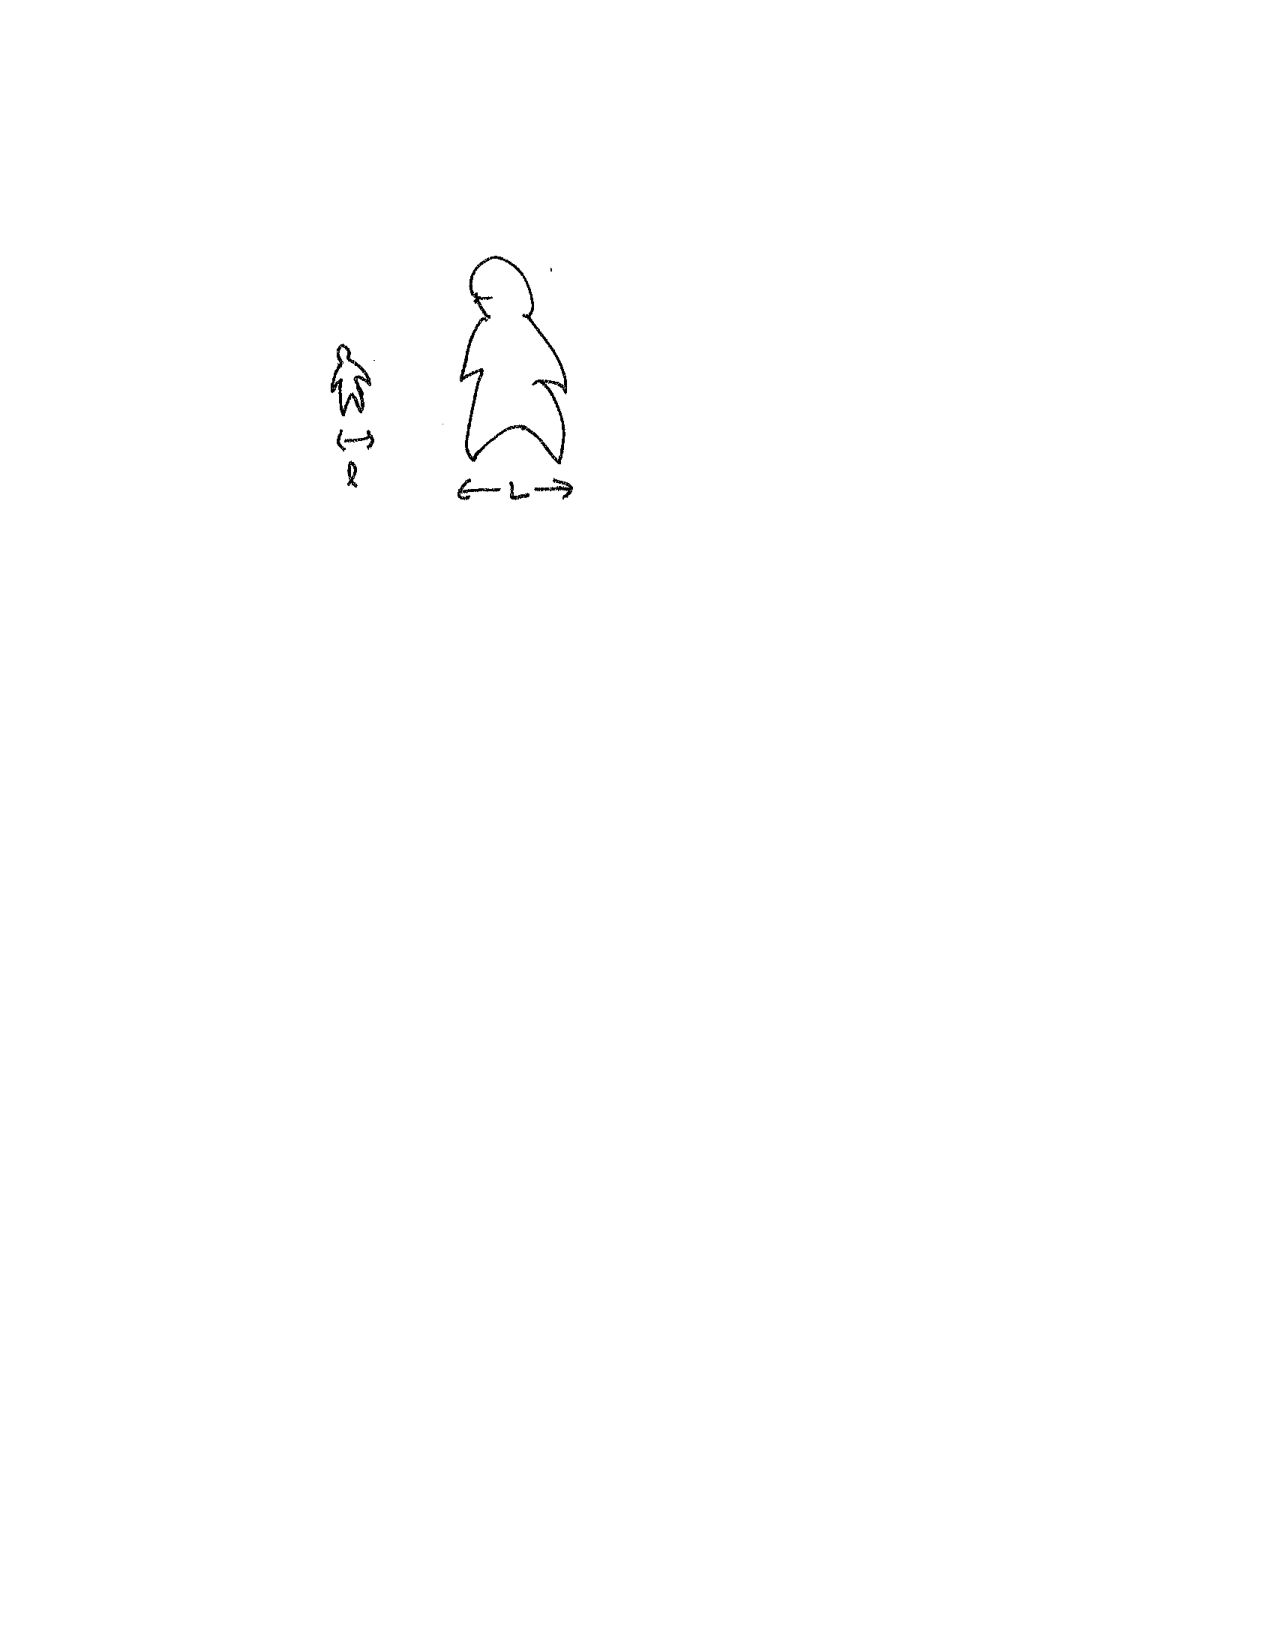
\includegraphics[width=.5\textwidth]{figures/lec01_allometry.pdf}
%     \caption{Two mathematically similar people.}
%     \label{fig:lec1_allometry}
% \end{figure}
\begin{marginfigure}%[th]
    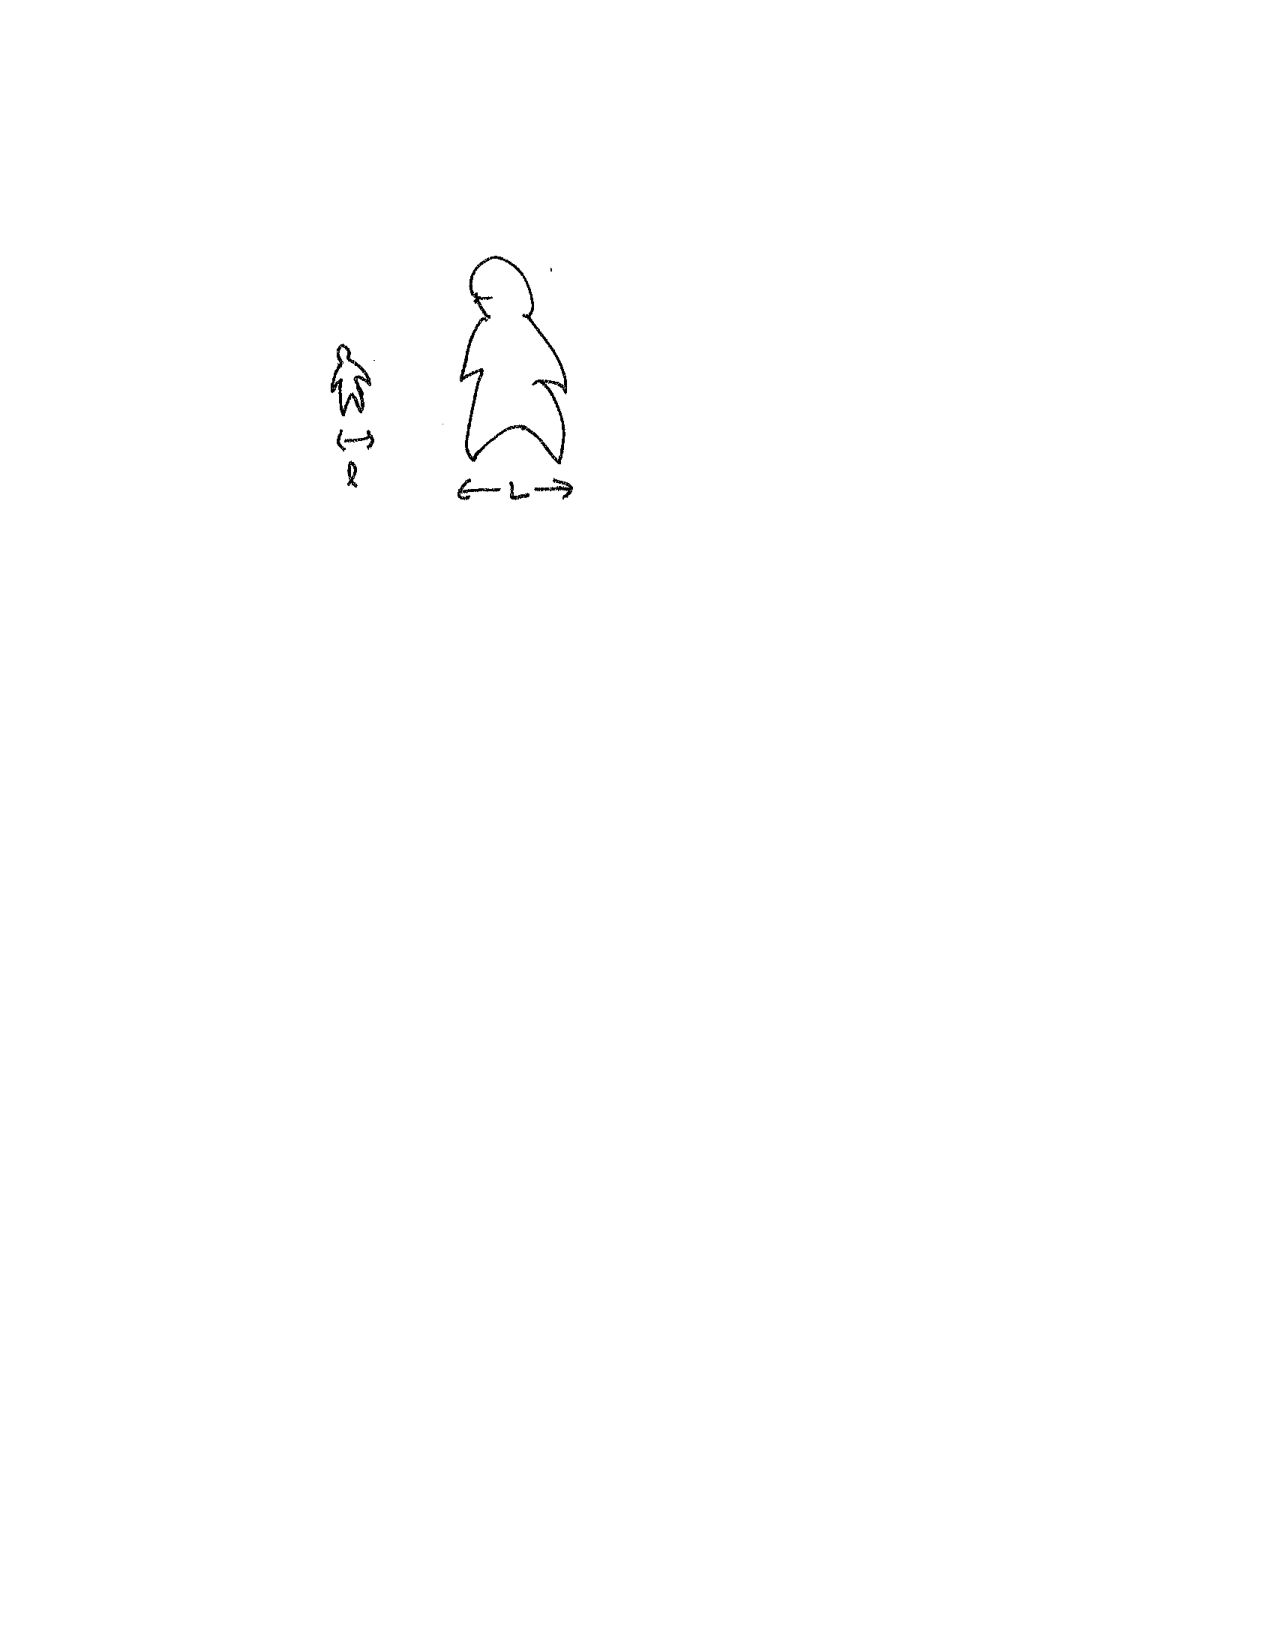
\includegraphics[width=.5\textwidth]{figures/lec01_allometry.pdf}
    \caption{Two mathematically similar people.}
    \label{fig:lec1_allometry}
\end{marginfigure}


\begin{exercise}
If both people exercised at the same rate, which one loses more absolute weight? By how much? Let us assume that weight loss is primarily from the conversion of organic molecules into carbon dioxide. 
\end{exercise}

\begin{exercise}
David Hu won his first IgNobel prize for determining that mammals take about 21 seconds to urinate, largely independently of their size\footnote{I learned about this in his excellent popular science book, \emph{How To Walk on Water and Climb Up Walls} by David Hu.}. Can you use dimensional analysis to argue why this would be the case? It may be helpful to refer to the paper\autocite{doi:10.1073/pnas.1402289111}. As you read it, figure out which terms are negligible (and in what limits), identify the assumptions of the mathematical model (scaling of the bladder and urethra), and prove the approximate scaling relation. Make a note to yourself of which steps were non-trivial and where one may have naively mis-modeled the system. By the way, David Hu won a second IgNobel prize for understanding wombats' cubical poop.
\end{exercise}

The above exercise on mammalian urination is a good example of \emph{modeling}.\index{model} As physicists, we must identify and make a mathematical model for the most salient features of a problem. We must also be able to quantify the error from neglecting sub-leading contributions. As a rough model for scaling purposes, we can ignore viscosity and surface tension effects on human-sized mammals. For much smaller mammals, these effects become larger---the authors of the study note that mice tend to urinate droplets---in which case one can ignore the `inertial' $\frac{1}{2} \rho v^2$ term in Bernoulli's equation. For human-sized mammals, we may assume that steady state urination is given by Bernoulli's equation:
\begin{align}
  P + \rho g h = \frac{1}{2}\rho v^2 \ ,
\end{align}
where $P$ is the pressure from the bladder, $h$ is the column height of the urethra, $\rho$ is the mass density of urine, and $v$ is the velocity of the urine at the end of the urethra. Let us simplify to the condition where urination is purely driven by gravity---that is, the bladder does not exert any additional pressure, $P=0$. You can now show that the total urination time scales like the mass of the mammal to the one-sixth power, $\tau \sim M^{1/6}$. That is, the urination time has a very weak scaling dependence on how massive the mammal is.

\begin{exercise}
In August 2021, Ezra Klein interviewed Dr.~C\'eline Goudner about the \tacro{COVID-19} variant.~\cite{klein_2021} In the interview, Klein cited the statement that the Delta variant has $\mathcal O(1000)$ times the viral load than prior \tacro{COVID} strains. Goudner then interprets this in the following way: if the \tacro{CDC} defined `close contact' for prior strains as 15 minutes of being indoors with an infected invdividual without a mask, then the equivalent `close contact' time for the Delta variant is around \emph{one second}. What scaling assumptions go into that estimate? Some of these assumptions are not obvious to me: for example, parts of the respiratory have a fractal-like structure that would lead me to suspect fractal scaling dimensions for surface area. \acro{Remark}: Just because you know dimensional analysis, that does not make you a medical, healthcare, or public policy expert.\footnote{Early in the \tacro{COVID-19} pandemic, many physicists became armchair  modelers of epidemics. Some of this was driven by hubris about our mathematical intuition. Many of the physicists lost interest when their models aligned poorly with what actually happened.} 
\end{exercise}

The following exercises draw from an article by Nicole Meyer-Verneta and Jean-Pierre Rospars in the American Journal of Physics\autocite{doi:10.1119/1.4917310} and the references therein.
 \begin{exercise}
 Estimate the expected velocity of an All Terrain Armored Transport (\tacro{AT}-\tacro{AT})\footnote{\url{https://starwars.fandom.com/wiki/All_Terrain_Armored_Transport}} of characteristic height $L$. You can assume that the walking behavior is based on a pendulum. \acro{Answer}: $v \sim \sqrt{Lg}/2\pi$.
 \end{exercise}


 \begin{exercise}
 Based on the density $\rho$, the force-per-cross-sectional area $\sigma$, and the maximum rate of energy consumption per unit mass $b$, one may estimate the `sprint' velocity of an animal of length $L$. This sprint velocity is conveniently described with respect to the dimensionless `body lengths per time,' $v_\text{spr}/L$.

Remarkably, for over 20 orders of magnitude in animal length $L$, the value of $v_\text{spr}/L$ is within an order of magnitude of 10/sec:
\begin{center}
 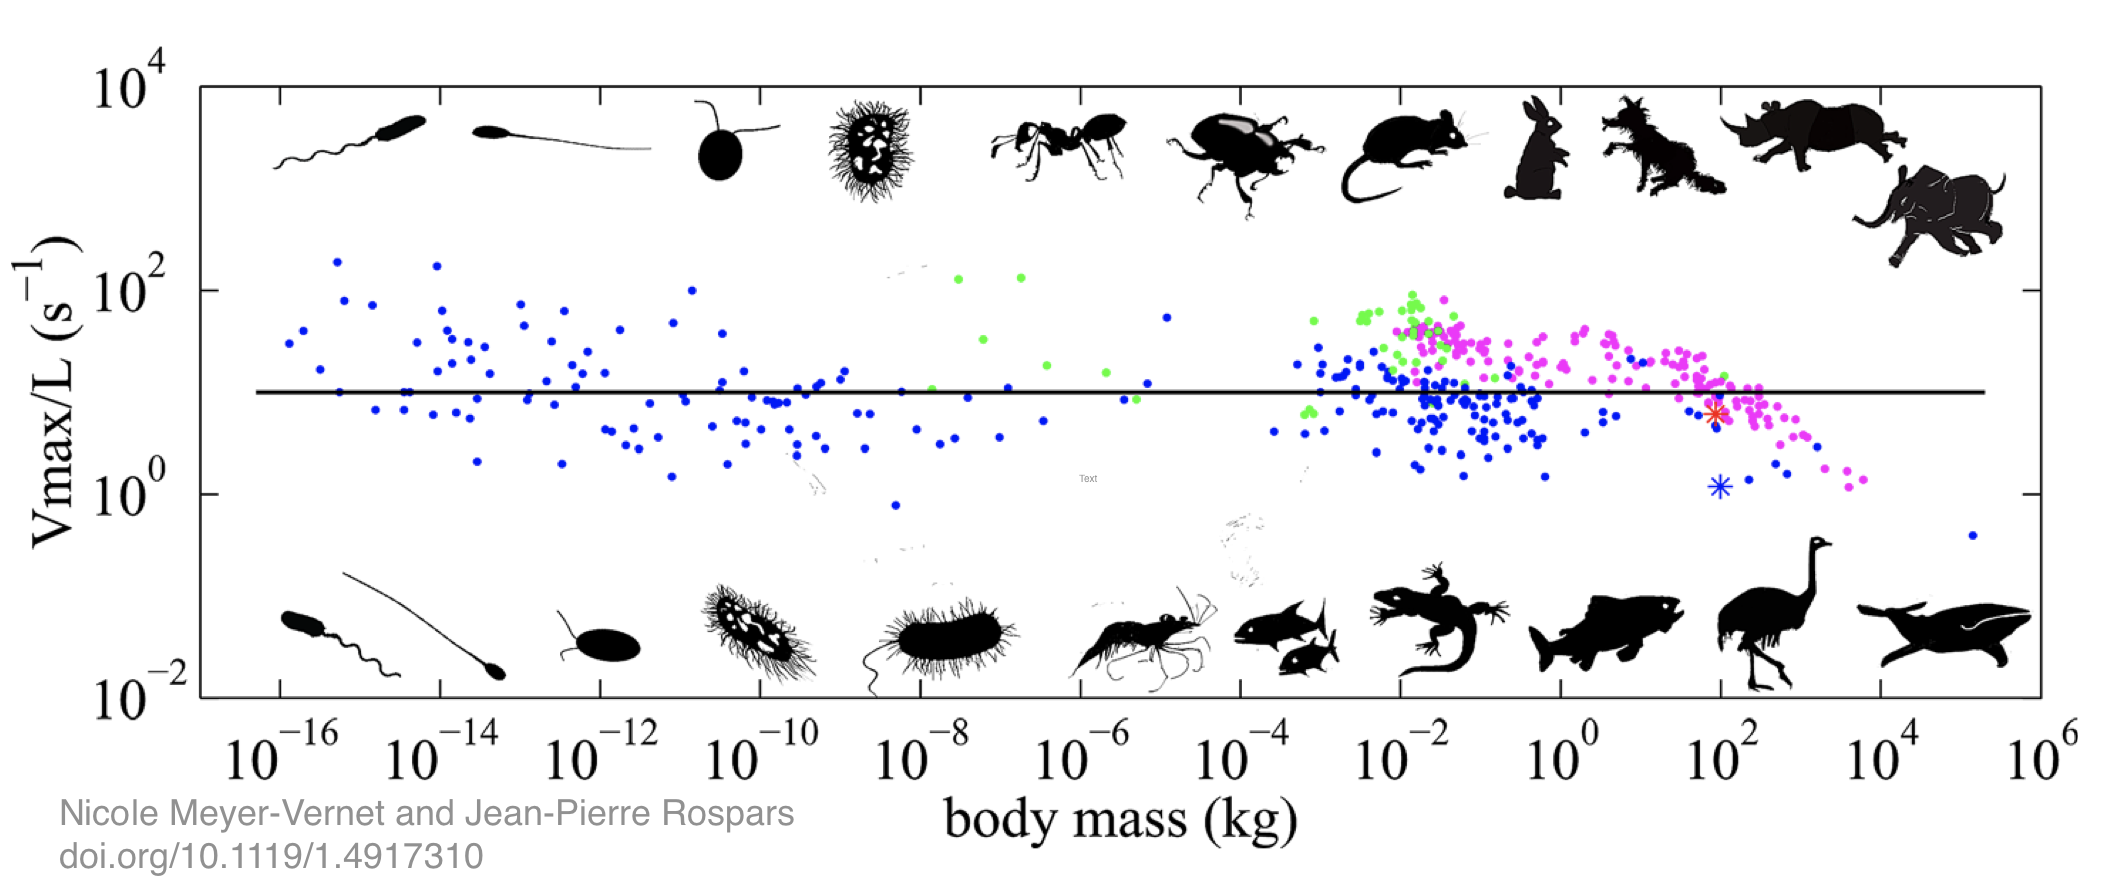
\includegraphics[width=\textwidth]{figures/allometry_meyer-verneta.png}
\end{center}
% \textfig[1]{figures/allometry_meyer-verneta.png}{Image from Meyer-Verneta and Rospars.~\cite{doi:10.1119/1.4917310}}{fig:allometry_meyer-verneta}


Argue from dimensional analysis that $v_\text{spr}/L \sim b\rho/\sigma$. (This is the easy part.) It turns out that there are simple physical principles for each of these terms to be roughly constant for all life on Earth (this is the more subtle part); see the article for a discussion.
\end{exercise}

\begin{exercise}
The height of trees. How does the maximum height of a tree, $L$ scale with the diameter of its cross section, $d$? For an argument that $L\sim d^{3/2}$, see Thomas McMahon's article ``The Mechanical Design of Trees'' in \emph{Scientific American}\footnote{\url{https://www.jstor.org/stable/24949846} (1975)}. McMahon was the first to propose a physical explanation for the observed scaling law that the metabolic rate of an animal scales like the characteristic size to the 3/4 power. A nice bibliography of his work can be found in \emph{Annual Review of Biomedical Engineering}.~\autocite{doi:10.1146/annurev.bioeng.3.1.0}
\end{exercise}



\part{Linear Algebra}

This part is a review of undergraduate-level linear algebra and forms the core of the Physics 17 course. The material is likely to be very familiar for graduate students in physics, but we provide it here to emphasize the use of indices and the `unified picture' of vector spaces and their duals that appear in the study of Green's functions. Physics 231 students can start with Chapter~\eqref{ch:P231:summary} and refer back as necessary.


\chapter{The Basics}\label{ch:basics}


\section{Pre-conceptions}

If this were a mathematics course, then we would start by very carefully defining words like \emph{vector} and \emph{matrix}. As a physics student, you already have a working definition of these words. It is probably something like this:
%
\begin{quote}
A vector has a magnitude and a direction. We write a vector as an array of three numbers arranged in a column. A matrix is an array of nine numbers arranged in a $3\times 3$ block. There is a rule for how to apply (multiply) the matrix to the vector to produce a new vector.
\end{quote}

The problem is that you already know too much to learn linear algebra as a mathematics student. You have already seen the tip of the iceberg and so have preconceptions about what vectors are and how they work. You may remember from freshman mechanics that forces are vectors. So are momenta and velocities. You may also recall the idea of a force field---like the electric field---which is actually a whole bunch of vectors: one for each point in space. Examples of matrices are a little more subtle: you may recall that you can represent rotations as matrices. Speaking of rotations, there was another thing that showed up called the moment of inertia \emph{tensor}. It looked like a matrix, but we never called it the ``moment of inertia matrix.'' What the heck is a tensor, anyway?

And so, you see that starting this course like a mathematics course could cause trouble. The mathematics professor would start by defining a vector. That definition will say nothing about magnitudes or directions, and will not even say anything about arrays of numbers. That definition will clash with the hard-earned intuition that you built from your physics education thus far. It will be perplexing, and may make you feel rather unhappy. What do these mathematicians know, anyway? Or maybe its the physics that is wrong, or have we just completely misunderstood everything and we are just now noticing that we are hopelessly lost? We begin to spiral into a black hole of confusion.

\begin{quote}
Fortunately, \emph{this is not a mathematics course.}
\end{quote}

As a consequence, we will not give a rigorous definition of a vector. We start with a familiar definition of vectors and lay out which qualities are general, and which properties are specific. Then we will come to appreciate the approximation that ``\emph{everything is a vector}.'' So let us start with something comfortably familiar, even though it constitutes only the simplest example of a vector.


\section{Real Three-Vectors}

Let us write $\vec{v}$ to be a vector. This is a standard convention for writing a vector. In this course we will use a few different notations for vectors according to convenience. Notation is neither physics nor mathematics, it is simply a shorthand for a physical or mathematical idea. 

% At this point, you may wonder \emph{what is a vector, anyway?} Maybe a vector is a column with three numbers that represent coordinates in three-dimensional space:
In fact, let us focus on a particular type of vector: \textbf{real three vectors}\index{three vector}. These are the familiar vectors that we can write as a column of three numbers that effectively represent the coordinates in three-dimensional space:
\begin{align}
    \vec{v} = 
    \begin{pmatrix}
        x\\ y\\ z
    \end{pmatrix} \ ,
\end{align}
where $x$, $y$, and $z$ are real numbers. These numbers are called the \textbf{components} of the vector $\vec{v}$.

\begin{exercise}
There is something very perverse about this ``vector.'' The variable names $x$, $y$, and $z$ imply that $\vec{v}$ is something that physicists like to call a ``position vector.'' If you say this to a mathematician they will vomit. By the end of this course, you should appreciate why the notion of a position vector makes no sense. \emph{Hint:} You may have some intuition for this already: a velocity vector tells you about the instantaneous motion of a particle relative to its present position. Try to write the analogous statement for a ``position vector.\footnote{I am not a mathematician, but you see that even I have to write ``position vector'' in condescending quotation marks. In lecture I use even more condescending air quotes.}''
\label{ex:position:vector}
\end{exercise}

This three-dimensional space is called [three-dimensional] \textbf{real space} and we write it as $\RR ^3$. This is because a vector is an element of three-dimensional real space specified by \emph{three} real numbers. 

Three-dimensional real space is an example of a \textbf{vector space}\index{vector space}, which is just a stupidly formal way of saying that it is where vectors live. Vectors are \emph{elements} of a vector space. A vector space is the set of all possible allowed vectors of a given type. For $\RR ^3$, the vector space is composed of all possible triplets of real numbers. 


\begin{example} It should be no surprise that we can imagine real two-dimensional space, $\RR ^2$. This is a vector space where each vector may be written as two real numbers. You can also imagine writing real four-dimensional space, $\RR ^2$, or complex two dimensional space, $\mathbbm{C}^2$. 
\end{example}

From the above example, you should have some intuition for what the \textbf{dimension}\index{dimension} of a vector space means: the dimension counts how many numbers you need to specify a vector. For real vector spaces, $\RR ^d$, the dimension is the number $d$. We will always assume that $d$ is a positive integer.\sidenote{The notion of a non-integer-dimensional space does show up occasionally. These do not even have to be particularly exotic: you can look up the dimension of a fractal.}





\section{Vectors and Numbers}

% We now make some general statements about vector spaces. These apply to all vector spaces, not just $\RR ^3$, but you can keep $\RR ^3$ in mind as we go over them. 

We should be clear that there are now two different kinds of objects: \emph{vectors} and \emph{numbers}. We will have all sorts of notation for vectors, but let us write them with a boldfaced Roman letter for now, e.g.~$\vec{v}$. We typically write numbers as lowercase italicized Roman letters like $a$ or sometimes Greek letters like $\alpha$. These two types of objects are similar, except vectors do not have a built-in definition for multiplication, see Table~\ref{table:vectors:numbers}.

\begin{table}
    \renewcommand{\arraystretch}{1.3} % spacing between rows
    \centering
    \begin{tabular}{ @{} lll @{} } \toprule % @{} removes space
         & Vectors & Numbers 
        \\ \hline
        Addition (commutative, associative) & \cmark & \cmark 
        \\
        Additive null element & $\vec{0}$ & 0
        \\
        Additive inverse element & $\vec{v} + (-\vec{v}) = 0$ & $a + (-a) = 0$
        \\
        Multiplication of two of these objects & \textcolor{red}{\xmark} & \cmark 
        \\
        Multiplication by a number (distributive) & \cmark & \cmark \,(same as above)
        \\
        Collection of all allowed objects (space) & vector space & field (``numbers'') 
        \\
        Example of a space & $\RR ^3$ & $\RR $
        \\ \bottomrule
    \end{tabular}
    \caption{
        What you can do with vectors compared to numbers. The glaring difference is that we cannot multiply two vectors. We will need to invent additional mathematical structure to define vector multiplication.
        \label{table:vectors:numbers}
  }
\end{table}

You already know everything there is to know about numbers.\sidenote{Formally, what I mean by `number' is what mathematicians call a \emph{field}. This simply means some objects where one can add, subtract, multiply, and divide as you would expect. This term is a little tedious for us because physicists usually mean something else when they say `field.' Usually we mean something like the electric field or the field associated with the Higgs boson.} Most relevant is that you can multiply numbers with each other (including division, the inverse of multiplication) and you can add them together (including subtraction). For the first part of this course, we will focus on real numbers, $\RR $. Later we will also allow for complex numbers, $\mathbbm{C}$. 

Like numbers, vectors can be added and subtracted. In fact, vector arithmetic turns out to be very similar to `number arithmetic.' However, unlike numbers, there is no obvious definition for vector multiplication. This leads to the idea of \emph{defining} functions for various kinds of vector multiplication. Linear algebra is the study of a particular class of these functions. The dot product, for example, which takes two vectors and returns a number, is something we have to ``make up'' and attach to a vector space.



\section{Notation: Indices}

One theme in this course is that we will repeatedly refine our notation to suit our needs. Let us introduce an \emph{index} notation where we write the components of vectors $\vec{v}$ and $\vec{w}$ as follows:
\begin{align}
    \vec{v}
    &=
    \begin{pmatrix}
        v^1 \\ v^2 \\ v^3
    \end{pmatrix}
    &
    \vec{w}
    &=
    \begin{pmatrix}
        w^1 \\ w^2 \\ w^3
    \end{pmatrix} \ .
\end{align}
We see that a boldfaced Roman letter, $u$, corresponds to a vector. The \emph{components} of the vector are $u^1$, $u^2$, $u^3$. The ``$x$-component'' of $\vec{u}$ is called $u^1$: we use the same letter as the vector, but italicized rather than boldfaced. The upper index is \emph{not} some kind of power, it simply means ``the first component.'' 

\begin{example}
If you see $\vec{s}$, this is understood to be a vector that has multiple components. If it is a three-vector, it has three components. If you see $s^2$, then this means that this is the \emph{second component} of the vector $\vec{s}$. The component of a vector is a number. 
\end{example}

You may worry that this notation introduces ambiguity. If we see $q^2$, is this the square of some number $q$, or is it the second component of some vector $\vec{q}$? The answer depends on context. You should avoid choosing variable names where there is ever the potential for ambiguity. If you have a vector that you call $\vec{q}$, then do not use the letter $q$ for anything else.

\sidenotetext{It is a personal pet peeve of mine that some first year courses for physics majors are sloppy about this. The instructors should know that they are building the foundation for understanding quantum mechanics and special relativity: they should start developing \emph{good} mathematical habits early on. }
\begin{example}
Some courses\sidenotemark write vectors as rows: $\vec{v}=\begin{pmatrix}
    v^1 & v^2 & v^3
\end{pmatrix}$ \ . Even more annoying to me, they may write everything with a lower index, $\vec{v}=\begin{pmatrix}
    v_1 & v_2 & v_3
\end{pmatrix}$ \ . There is nothing \emph{wrong} with this, certainly in classes where there is only one type of vector. However, in order to make full use of linear algebra, we need to treat so-called column vectors separately from so-called row vectors. To do this, we introduce a new set of notation where the heights of the indices are important. Eventually we will get rid of the notion of rows versus columns altogether---but the notion of upper and lower index will remain.
\end{example}


You know from $\RR ^3$ that you can add together any two vectors $\vec{v}$ and $\vec{w}$.
% 
Let us call this sum $\vec{u}$ so that $\vec{u}\equiv \vec{v}+\vec{w}$. Then we can succinctly write the components of $\vec{u}$ in one line:
\begin{align}
    u^i = v^i + w^i \ .
    \label{eq:u:v:plus:w:index}
\end{align}
The variable $i$ is called an \textbf{index}\index{index}. What values does the index take? In this example, it is 
clear that \eqref{eq:u:v:plus:w:index} holds for $i=1,2,3$. That is, $i$ takes values from 1 to the dimension of the space. The typical convention is that we do not have to state the range of index values because it should be understood from the space itself. 

With that in mind, it should be clear that if $\vec{q}$ is the difference of two vectors, then the components of $\vec{q}$ may be succinctly written:
\begin{align}
\vec{q} &= \vec{v}-\vec{w}    
&
&\Leftrightarrow
&
q^i &= v^i - w^i \ .
\end{align}
In fact, as physicists we typically use the two statements above interchangeably. If you know the components of a vector, then you know the vector.


\section{Arithmetic and linear combinations}

All vector spaces allow addition and subtraction. This is defined component-wise. The sum of $\vec{v}$ and $\vec{w}$ is
\begin{align}
    \vec{v}+\vec{w} = 
    \begin{pmatrix}
        v^1 + w^1\\
        v^2 + w^2\\
        v^3 + w^3
    \end{pmatrix} \ .
\end{align}
What this means is that the \emph{sum} of two vectors is also a vector. That means that if $\vec{v}$ and $\vec{w}$ are vectors in $\RR ^3$, then $(\vec{v}+\vec{w})$ is a vector in $\RR ^3$. The components of the vector $(\vec{v}+\vec{w})$ are simply the sum of the components of $\vec{v}$ and $\vec{w}$. 
% 
A few formal properties that generalize to all vector spaces:
\begin{itemize}
    \item Vector addition is associative. This means that in the sum $\vec{v}+\vec{w}+\vec{u}$, it does not matter if you add $(\vec{v}+\vec{w})$ first and then add $\vec{u}$, or if you take $\vec{v}$ and then add it to $(\vec{w}+\vec{u})$. This is the kind of `obvious' property that we tend to take for granted.
    \item Vector addition is commutative. $\vec{v}+\vec{w} = \vec{w}+\vec{v}$. This is also kind of obvious. But recall that matrix multiplication is not commutative.
    \item There is a zero vector, $\vec{0}$, that does leaves any other vector unchanged under addition. $\vec{v}+\vec{0} = \vec{v}$. This should be totally obvious. The components of $\vec{0}$ are obviously all zero.
    \item There is an additive inverse (negative vectors). If $\vec{v}$ is a vector, then $-\vec{v}$ is a vector and satisfies $\vec{v}+(-\vec{v}) = \vec{0}$.
\end{itemize}
\begin{example}
The first property implies that once you have identified one vector in a vector space, $\vec{v}$, then you can immediately have an infinite number of vectors. This is because $2\vec{v} = \vec{v}+\vec{v}$ must also be a vector. Then $3\vec{v} = 2\vec{v}+\vec{v}$ must also be a vector. And so forth.
\end{example}

We get another type of operation ``for free'' with a vector space. This is called scalar multiplication or \emph{rescaling}.

% You can multiply vectors by numbers. This is called rescaling or scalar multiplication. All the usual properties of multiplication by numbers holds: associativity, commutivity, distributive law.


\section{Rescaling: multiplication by a number}

Another operation that exists in a vector space is rescaling: we multiply a vector by a number. 
Let $\alpha$ be a number. If you want to nitpick, let us restrict $\alpha$ to be a real number. If we have a vector $\vec{v}$ with components $v^i$, then $\alpha \vec{v}$ is also a vector.\sidenote{``Also a vector'' means that it is also an element of the vector space; so $(\alpha\vec{v})$ is an element of $\RR ^3$ is $\vec{v}$ is an element of $\RR ^3$. } The components of $\alpha \vec{v}$ are
\begin{align}
    (\alpha v)^i = \alpha v^i \ ,
\end{align}
by which we mean
\begin{align}
    (\alpha\vec{v})
    =
    \begin{pmatrix}
        \alpha v^1 \\
        \alpha v^2 \\
        \alpha v^3 
    \end{pmatrix} \ .
\end{align}
The parenthesis on the left-hand side is sloppy notation to mean ``the vector that is the vector $\vec{v}$ rescaled by the number  $\alpha$.'' Another way of saying this is that there is a vector $\vec{w}\equiv \alpha\vec{v}$ whose components are $w^i = \alpha v^i$.

\begin{example}
Let us do one explicit example with numbers. Suppose the vectors $\vec{v}$ and $\vec{w}$ have components
\begin{align}
    \vec{v} &=
    \begin{pmatrix}
    \phantom{+}4.2\\
    -2.6\\
    \phantom{+}7.0        
    \end{pmatrix}
    &
    \vec{w} &=
    \begin{pmatrix}
    \phantom{+}5.3\\
    \phantom{+}2.1\\
    -2.5        
    \end{pmatrix} \ .
\end{align}
I can rescale each vector by different numbers: $\alpha = 10$, $\beta = 2$. We can consider the vector that comes from adding these rescaled vectors:
\begin{align}
    \vec{u} \equiv \alpha \vec{v} + \beta \vec{w} \ .
\end{align}
The second component of $\vec{u}$ is $u^2 = -26 + 4.2 = -21.8$.
\end{example}

At this point it is useful to define some jargon. A \textbf{scalar}\index{scalar} is a number. This is in contrast to vectors (and matrices and tensors) which we can think of as arrays of numbers. In fact, every time you see the word scalar, you should just think ``number.'' Another name for `rescaling a vector by a number' is \emph{scalar multiplication}.

\section{Linear Combination and Span}
\label{sec:linear:combination:and:span}

Based on our rules for vector space arithmetic, we know that if $\vec{v}$ and $\vec{w}$ are two vectors in our vector space and if $\alpha$ and $\beta$ are any two numbers, then
\begin{align}
    \alpha\vec{v} + \beta\vec{w} 
\end{align}
is also a vector in our vector space. We call any such sum---for any values of $\alpha$ and $\beta$---a \textbf{linear combination}\index{linear combination} of the vectors $\vec{v}$ and $\vec{w}$. You can of course generalize to the linear combination of more than two vectors, say
\begin{align}
    \alpha\vec{v} + \beta\vec{w} + \gamma\vec{u} \ .
\end{align}

Given some number of vectors---$\vec{v}$ and $\vec{w}$---you can ask what are all of the possible vectors that you can form from the linear combination of those vectors? This is a vector space.\sidenote{You may want to convince yourself that this satisfies the requirements of vector space arithmetic.} We say that this vector space is \textbf{spanned} by the vectors $\vec{v}$ and $\vec{w}$. We call this vector space $\text{Span}(\vec{v},\vec{w})$. You can extend this to even more vectors, $\text{Span}(\vec{v}, \vec{w}, \vec{u},\cdots)$.

\begin{exercise}
Show that the vector space spanned by $\vec{v}$ and $\alpha\vec{v}$ is the same as the vector space spanned by $\vec{v}$.
\end{exercise}

\begin{exercise}
If $\RR ^3$ is the space of vectors with three real components, argue that the span of any four vectors is at most $\RR ^3$ but possibly a subset of $\RR ^3$. Give an example where the span of four vectors is $\RR ^2$. 
\end{exercise}


\section{Basis vectors: an illustrative example}

Let us push this idea further. It is useful to start with an example. For simplicity, let us focus on the two-dimensional plane, $\RR ^2$. A vector in $\RR ^2$ looks like this:
\begin{align}
    \vec{v} =
    \begin{pmatrix}
        v^1 \\ v^2
    \end{pmatrix} \ .
    \label{eq:v:v1:v2}
\end{align}
Any such vector may be written as the linear combination of the following two vectors:
\begin{align}
    {\bas{e}}_1 &=
    \begin{pmatrix}
        1 \\ 0
    \end{pmatrix}
    &
    {\bas{e}}_2 &=
    \begin{pmatrix}
        0 \\ 1
    \end{pmatrix} \ .
\end{align}
Indeed, it should be obvious that 
\begin{align}
    \vec{v} &= \alpha {\bas{e}}_1 + \beta {\bas{e}}_2
    & \text{with}&
    &\alpha &= v^1
    &\beta &= v^2 \ .
    \label{eq:natural:cartesian:basis}
\end{align}
In other words, these `special' vectors ${\bas{e}}_{1,2}$ satisfy:
\begin{enumerate}
    \item Any vector in $\RR ^2$ may be written as a linear combinations of ${\bas{e}}_{1,2}$. We showed this because $\vec{v}$ in the above discussion could be any vector in $\RR ^2$. Thus $\text{Span}({\bas{e}}_{1},{\bas{e}}_{1})=\RR ^2$.
    \item The coefficients in the linear combination are precisely the components of the vector $\vec{v}$. Soon we will see that this observation is actually backwards: it is the choice that ${\bas{e}}_{1}$ are special that defines the components of a vector.
\end{enumerate}

It should be obvious that any pair of vectors that ``aren't pointing in the same direction'' can span the entire space $\RR ^2$. 
\begin{exercise}
What does ``aren't pointing in the same direction'' mean in this context? Use $\vec{v}$ and $\alpha\vec{v}$ in your answer.
\end{exercise}
We could try a different pair of vectors and consider its linear combinations:
\begin{align}
    \vec{f}_1 &=
    \begin{pmatrix}
        1\\1
    \end{pmatrix}
    &
    \vec{f}_2 &=
    \begin{pmatrix}
        0\\1
    \end{pmatrix} \ .
\end{align}
Then the vector $\vec{v}$ may be written as $\vec{v} = \alpha \vec{f}_1+ \beta\vec{f}_2$. To find $\alpha$ and $\beta$, we can simply plug in the components of $\vec{v}$ and $\vec{f}_{1,2}$ so that:
\begin{align}
    v^1 &= \alpha -\beta
    &
    v^2 &= \alpha \ .
\end{align}
In other words,
\begin{align}
    \vec{v} = (v^2) \vec{f}_1 + (v^2 - v^1)\vec{f}_2 \ .
\end{align}
These coefficients $\alpha = v^2$ and $\beta = v^2 - v^1$ may be written  in shorthand. Let's suggestively write
\begin{align}
    \vec{v} = 
    \begin{pmatrix}
        v^2\\
        v^2 - v^1
    \end{pmatrix}_{\vec{f}} \ ,
\end{align}
where we use the subscript $\vec{f}$ to mean ``coefficients with respect to $\vec{f}_{1,2}$. This looks just like a two-component vector, doesn't it?

\begin{exercise}
Let $\vec{v} \in \RR ^2$ be the following vector in two-dimensional real space:
\begin{align}
    \vec{v}=
    \begin{pmatrix}
        3\\2
    \end{pmatrix} \ .
\end{align}
Here are two vectors that span $\RR ^2$:
\begin{align}
    \vec{g}_1 &=
    \begin{pmatrix}
        2\\1
    \end{pmatrix}
    &
    \vec{g}_2 &=
    \begin{pmatrix}
        -1\\ \pp 0
    \end{pmatrix} \ .
\end{align}
What are the coefficients $\alpha$ and $\beta$ so that $\vec{v} = \alpha \vec{g}_1 + \beta \vec{g}_2$?  \emph{Answer}: $\alpha = 2$ and $\beta = 1$. 
\end{exercise}


What we're getting at is the following.  Define a set of vectors that span a space. We will call this set of vectors a \textbf{basis}\index{basis} of that space---we'll give a slightly more formal definition below. Any vector in the space can be written as a linear combination of basis vectors. For example, if $\vec{b}_{1,2}$ are a basis of $\RR ^2$, then for any vector $\vec{v}\in\RR ^2$ we may write
\begin{align}
    \vec{v} = \alpha \vec{b}_{1} + \beta \vec{b}_2 \ .
\end{align}
Then we have encoded all of the data of vector $\vec{v}$ into the coefficients $(\alpha, \beta)$. In fact, let me be more economical with my symbols and change notation a bit and write $(\alpha^1, \alpha^2) \equiv (\alpha,\beta)$ so that
\begin{align}
    \vec{v} = \alpha^1 \vec{b}_{1} + \alpha^2 \vec{b}_2 \ .
    \label{eq:R2:vec:v:in:b:components:lincomb}
\end{align}
Then I can write the information encoded in $\vec{v}$ as a column, which I will write with a subscript $b$ to distinguish it from the ``actual'' vector components, \eqref{eq:v:v1:v2}:\sidenote{We will soon see that the there is nothing holy about \eqref{eq:v:v1:v2}.}
\begin{align}
    \vec{v} = 
    \begin{pmatrix}
        \alpha^1\\
        \alpha^2
    \end{pmatrix}_{\vec{b}} \ .
    \label{eq:R2:vec:v:in:b:components}
\end{align}
The last two equations mean exactly the same thing. Now here's something cute: we can treat the two-component array\sidenote{I'm trying not to call it a vector.} on the right-hand side of \eqref{eq:R2:vec:v:in:b:components} as if it were a vector. We can do vector arithmetic on it. If we have two vectors with ``$\vec{b}$ basis components''
\begin{align}
    \vec{v}&=
    \begin{pmatrix}
        \alpha^1\\
        \alpha^2
    \end{pmatrix}_{\vec{b}} 
    &
    \vec{w}&=
    \begin{pmatrix}
        \beta^1\\
        \beta^2
    \end{pmatrix}_{\vec{b}}  \ ,
\end{align}
Then we could take linear combinations of the two with respect to two numbers $a$ and $b$:
\begin{align}
    a\vec{v} + b\vec{w} =
    (\alpha^1+\beta^1) \vec{b}_{1} + (\alpha^2+\beta^2) \vec{b}_2
    =
    \begin{pmatrix}
        \alpha^1 + \beta^1 \\
        \alpha^2 + \beta^2
    \end{pmatrix}_{\vec{b}} \ .
    \label{eq:linear:combination:in:b:basis}
\end{align}

If $\vec{v}$ and $\vec{w}$ span $\RR ^2$, then any vector in the vector space may be written as a linear combination of the form \eqref{eq:linear:combination:in:b:basis}. This means we may use the ``$\vec{b}$ basis components'' as equivalent ways of encoding a vector as the natural description \eqref{eq:v:v1:v2}. But wait a moment: what is so ``natural'' about \eqref{eq:v:v1:v2}? 

If we reverse the argument for the $\vec{b}$ basis, then we see that the ``natural'' components of the vector $\vec{v}$ in \eqref{eq:v:v1:v2} are simply the coefficients of the linear combinations of the basis vectors ${\bas{e}}_{1,2}$ in \eqref{eq:natural:cartesian:basis}. What made the basi vectors ${\bas{e}}_{1,2}$ so special, anyway? Nothing at all. 

What we've come to is that we the \emph{components} of a vector depend on the basis that we choose. In $\mathbb{R}^3$ we usually use the basis ${\bas{e}}_{1,2,3}$ where the vectors point respectively along the $\hat{x}$, $\hat{y}$, and $\hat{z}$ directions. It is kind of an ``obvious'' basis, though it completely depends on the $\hat{x}$, $\hat{y}$, and $\hat{z}$ directions having some intrinsic meaning. They often do not: we could set up our coordinate system however we wanted. In fact, \emph{nowhere} in our definition of a vector space did we even assume that a coordinate system exists!

Indeed, it's the other way around: a choice of basis vectors \emph{defines} a `coordinate system' rather than the other way around.\sidenote{Though it really is dangerous to think about a vector space as having coordinates. We will see why when we talk about vector bundles and manifolds.} All of this begs for a re-definition.





\section{Basis vectors, formally}

A \textbf{basis} is a \emph{minimal set} of vectors that span a space. Here `minimal' means that if you remove any vector from the basis, then there are vectors in the space that cannot be written as a linear combination of the remaining vectors.

\begin{example}\label{eg:over:specified:basis}
Consider the following three vectors:
\begin{align}
    \vec{v} &=
    \begin{pmatrix}
        1\\0\\0
    \end{pmatrix}
    &
    \vec{w} &=
    \begin{pmatrix}
        0\\1\\0
    \end{pmatrix}
    &
    \vec{u} &=
    \begin{pmatrix}
        1\\-1\\0
    \end{pmatrix} \ .
    \label{eq:tvu:example:basis}
\end{align}
These three vectors are \emph{not} a basis for a subspace because there are vectors that are linear combinations of $\vec{v}$, $\vec{w}$, and $\vec{u}$ that can be equivalently written as a linear combination of just $\vec{v}$ and $\vec{u}$, for example.
% 
To see this, consider the vector
\begin{align}
    \vec{t} = 4\vec{v} + 2\vec{w} + 3\vec{u} 
    =
    \begin{pmatrix}
        \pp 7 \\ -1 \\ \pp 0
    \end{pmatrix} \ .
\end{align}
This may equivalently be written as
\begin{align}
    \vec{t} = 7\vec{v} - \vec{w} \ .
\end{align}
Indeed, there are an infinite number of ways to write $\vec{t}$. Because $\vec{v} - \vec{w} + \vec{u} = 0$, you can add any multiple of this linear combination to $\vec{t}$ to leave $\vec{t}$ unchanged.
\end{example}

The \textbf{dimension} of a vector space is the number of vectors in the basis. In the example above, the vector space spanned by linear combinations of $\vec{v}$, $\vec{w}$, and $\vec{u}$ has dimension two. This is because you only need two vectors write any vector in the space as a linear combination. If you drew all of the vectors in this subspace as arrows with their base at the origin, then the arrow heads with all live on the $xy$-plane.

Here are some \emph{obvious} statements\sidenote{This means: if they are not immediately apparent, stop and think about it to make sure you understand.}:
\begin{enumerate}
    \item The zero vector cannot be part of any basis.
    \item The dimension of a vector space does not depend on the choice of basis.
    \item If you have a proposed set of basis vectors but there is a \emph{non-trivial} linear combination of those vectors that sums to zero, then the set of vectors is not a basis. Here non-trivial means ``the coefficients are not all equal to zero.'' This should be evident from Example~\ref{eg:over:specified:basis}.
    \item If any two vectors in a proposed basis are proportional to one another, then this set of vectors is not a basis.
    \item The number of components $v^i$ to describe a vector is the dimension of the vector space.
    \item In the expansion of a vector as a linear combination of basis vectors, the coefficients are unique to the vector. That is: if $\vec{v} = \sum_i \alpha^i\vec{b}_i$ for a basis $\vec{b}_{1,2,3}$, then the set of numbers $(\alpha^1, \alpha^2, \alpha^3)$ uniquely defines $\vec{v}$. There is no other combination of coefficients in a linear combination that sum to $\vec{v}$. 
    \item When describing a vector, the \emph{coefficients} of the linear combination of basis vectors and the \emph{components} of a column vector with respect to that basis are identical. This is by definition. 
\end{enumerate}
The last point is poignant. You may have believed that a vector \emph{is} the column of numbers. We want to move away from this so that we may generalize our definition. A vector is a linear combination of basis vectors, where we are remaining agnostic about what the basis vectors are. Let me say this again: \emph{the column of numbers is not the vector, it is simply a representation of a linear combination of basis vectors. All the ``vector-ness'' is encoded in the basis vectors.}\sidenote{For a sneak peek of this, you may want to jump to Section~\ref{sec:sub:abstraction:basis}.}




What is less obvious is that at this point there is \emph{no preferred basis}. Any minimal set of vectors that span a vector space is a perfectly good vector. Suppose $\vec{b}_{1,2,3}$ is one such set for $\RR ^3$. We can write the vector with respect to the coefficients of the linear combination of  $\vec{b}_{1,2,3}$ basis vectors that reproduces it. If we had another basis, $\vec{b}'_{1,2,3}$, we could write the same vector with respect to a different linear combination of the $\vec{b}'_{1,2,3}$ basis. The components of these linear combinations, say $\alpha^i$ and $\alpha'^i$, will be different because the basis elements are different. However, they represent the same vector.

In your heart, you should feel anxious. You \emph{like} the ``obvious'' basis 
\begin{align}
    {\bas{e}}_1 &=
    \begin{pmatrix}
        1 \\ 0 \\ 0
    \end{pmatrix}
    &
    {\bas{e}}_2 &=
    \begin{pmatrix}
        0 \\ 1 \\ 0
    \end{pmatrix}
    &
    {\bas{e}}_2 &=
    \begin{pmatrix}
        0 \\ 0 \\ 1
    \end{pmatrix} \ .
\end{align}
We can even call this the Cartesian basis.
It seems so natural, we even gave these basis vectors little hats to remind us how much we like them! Stop and think about what you like about this basis. I guarantee you that all of those nice features invoke mathematical machinery that are \emph{not} included in a vector space. You may like that the Cartesian basis is orthogonal and each basis vector has unit length. To this I reply: \emph{how do you measure angle or length? These are not concepts that our vector space is equipped with.} You are, of course, correct that there \emph{is} a way to \emph{define} angle and length---but that is something additional that we have to impose on the space. We will get to this shortly.


\begin{example}\label{eg:polynomial:space}
Another surprising example of a vector space is the space of polynomials of finite degree. This means functions of the form
\begin{align}
    f(x) &= a^0 + a^1 x + a^2x^2 + \cdots a^N x^N \ .
\end{align}
Finite degree means that $N$ is some integer that is not infinity.\footnote{This may seem like a silly point, but one of the key `aha' ideas in this course will be that we can do linear algebra on the space of general functions where we allow $N\to \infty$.}
To be clear, our notation has become a bit ambiguous: here $x$ is a variable and $x^n$ means $x$ to the $n^\text{th}$ power. The coefficients $a^i$, on the other hand, are numbers and $i$ is an index. We can pick the following basis:
\begin{align}
    {\bas{e}}_0 &= x^0 = 1 &
    {\bas{e}}_1 &= x^1 = x &
    {\bas{e}}_2 &= x^2 &
    \cdots&&
    {\bas{e}}_N &= x^N &
\end{align}
These `basis vectors' are actually functions that are simple monomial powers of $x$. It should be obvious (there's that phrase again) that linear combinations of these basis vectors/functions can give any function $f(x)$ of degree up to $N$. It should also be obvious that the dimension of this space is $(N+1)$; don't forget to count the ${\bas{e}}_0$ vector.\par

For example, consider the polynomial $f(x) = 3+x^2$. The linear combination of basis vectors that gives this has $a^0 = 3$, $a^2 = 1$, and all other coefficients zero:
\begin{align}
    f(x) = 3{\bas{e}}_0 + {\bas{e}}_2 \ .
\end{align}
We could represent this vector/function as a column:
\begin{align}
    f(x) = \vec{f} = 
    \begin{pmatrix}
        3 \\
        0 \\
        1 \\
        0 \\
        \vdots  \\
        0
    \end{pmatrix}
\end{align}
where $\vec{f}$ is an $(N+1)$-component column of the numbers $a^i$.
\end{example}

\begin{exercise}
Consider a vector/function $\vec{f}$ with components $f^i$ in the polynomial space in Example~\ref{eg:polynomial:space}. Now consider the vector/function $\vec{f}' \equiv df/dx$. Write out an expression for the $i^\text{th}$ component of $\vec{f}'$. \emph{Hint}: for example, the $i=1$ component is $2f^2$.
\end{exercise}



\section{The meaning of column vectors}

The previous subsection on bases\footnote{The plural of `basis' is `bases,' pronounced \emph{bay-sees}, just like the plural of `axis' is `axes' pronounced \emph{axe-sees}.} is so important that we should really emphasize the mathematical edifice that we have reverse-engineered\footnote{Do you appreciate why I say `reverse engineered' here? In mathematics classes, one woud start with some postulates for what an abstract vector is and then your usual 3-component column vectors pop out as one silly example. We have started those 3-component column vectors and used their properties to motivate a general definition of what vectors are.}
\begin{enumerate}
    \item A vector is technically \emph{not} the column of numbers that we usually say it is. That column of numbers is simply a way of writing the \emph{components} of a vector.
    \item The components of a vector are simply the coefficients of the basis vectors in the linear combination of basis vectors that sum to the vector. That is: $v^i$ is defined by $\vec{v} = v^i {\bas{e}}_i$ where the ${\bas{e}}_i$ are a set of basis vectors that we all agree upon.
    \item I never had to say what the basis vectors \emph{are}. They can be anything where linear combinations of those things are still the same type of thing. In this way, we can treat the basis vectors abstractly.
\end{enumerate}
You may be used to vectors being forces, momenta, velocities, electric fields, and so forth. We want to be able to use the same machinery of linear algebra on more general objects: particles with quantum spin, functions, the perception of colors by the human eye, and so forth.


\begin{exercise}
What happens when we do not agree on a basis? Suppose you set up a basis. Stand up. Suppose you are facing north. Your feet are at the origin. If you spread your arms out, your right hand points in the direction of your first basis element ($x$-axis, pointing east), ${\bas{e}}_1$. Your nose points in the direction of your second basis element ($y$-axis, north), ${\bas{e}}_2$. Your head points in the direction of your third basis element ($z$-axis, skyward), ${\bas{e}}_3$.

However, your friend Riley approaches you from the northeast so Riley is facing southwest. Riley decides to set up their own basis, analogous to you. Their first basis element ${\bas{r}}_1$ points in the northwest direction, their second basis element ${\bas{e}}_2$ points in the southwest direction, and their third basis element ${\bas{e}}_3$ also points skyward. 

For simplicity, assume that the length of your basis vectors are all the same---even though we haven't defined what length means. Suppose you `measure' a vector with components $v^1 = 2$, $v^2=-1$, and $v^3=1.5$. This is a vector pointing southeast and upward. What components does Riley measure with respect to their basis?
\end{exercise}



In some physics classes there is an agreed upon notion that the basis vectors are 
\begin{align}
    \bas{e}_1 &= \hat x_1 = \hat i
    &
    \bas{e}_2 &= \hat y_1 = \hat j
    &
    \bas{e}_3 &= \hat z_1 = \hat k \ .
\end{align}
This is not one of those classes. Often this \emph{canonical} basis is the obvious one to use, and we will try to use it. However, in this class you must be able to accept that we want to \emph{abstract} away the identity of the basis vectors. The basis vectors simply carry the vector-ness of a vector so that we can focus only on dealing with the \emph{components}, which we write as columns of numbers.




\section{Operations that are not (yet?) allowed}

In these definitions, we make a big deal about how the sum of two vectors \emph{is also a vector}. Or how the rescaling of a vector by a number \emph{is also a vector}. This is in contrast to operations that are either not allowed or that do not produce vectors. An example of an operation that is not allowed is adding together vectors from two different vector spaces. The following proposed sum of a vector in $\RR ^3$ with  a vector in $\RR ^2$ does not make sense:
\begin{align}
    \begin{pmatrix}
        v^1\\ v^2 \\v^3
    \end{pmatrix}
    +
    \begin{pmatrix}
        w^1\\ w^2 
    \end{pmatrix}
    =
    \; ?
\end{align}
If you find yourself adding vectors from two different vector spaces, then you have made a mistake.

Another operation that requires care is rescaling a real vector by a complex number. If $\vec{v}$ is a vector in $\RR ^3$ and we try to multiply it by a complex number, $\alpha = 2+3i$, then the resulting ``vector'' is \emph{not} a vector in $\RR^3$:
\begin{align}
    (\alpha\vec{v})^i = (2+3i)v^i \notin \RR  \ ,
\end{align}
that is: the components of $\alpha\vec{v}$ are not real numbers, and so this cannot be an element of aa vector space that is \emph{defined} to have real components. Later on we will generalize to the case of \emph{complex vector spaces}, but we will treat that with some care.\sidenote{If you want to be fancy, you can replace `number' with the mathematical notion of a \emph{field}\index{field}. Both the real numbers and the complex numbers are examples of fields. In my mind a field is just a class of number, though mathematicians have fancier definitions.}

Thus far, we have introduced the \emph{nouns} of this course: vectors. We have identified a few \emph{verbs} that let us do things with these vectors:
\begin{enumerate}
    \item Addition takes two vectors in a vector space and returns a vector in the same vector space. 
    \item Rescaling takes a vector and a number and returns a vector in the same vector space.
\end{enumerate}
We can rewrite this in the language of \emph{mappings} (or \emph{functions}) as follows. Let $V$ be a vector space, say $V=\RR ^3$. Let us write $\RR $ mean [real] numbers. Then the above statements tell us that addition and rescaling can be thought of as maps:
\begin{enumerate}
    \item Vector addition: $V\times V \to V$
    \item Rescaling: $V\times \RR  \to V$ \ .
\end{enumerate}
Do not be intimidated by the $\times$ symbol here. This ``mapping'' notation means nothing more and nothing less than the statements above.

We now know everything there is to know about the vector space $\RR ^3$. We want to learn more about functions (maps) that involve this vector space. How can we combine vectors and numbers to produce other vectors and numbers? What about more complicated objects like matrices and tensors? 

\section{Euclidean three-space}

You may object: \emph{wait! I know there are more things you can do with three-vectors!} You remember that there are two types of vector multiplication that we use in physics. The \textbf{dot product} and the \textbf{cross product}. 

In $\RR ^3$, the \textbf{dot product} is a map $V\times V \to \RR $. That means it takes two vectors and returns a number. The particular number that it returns is typically \emph{defined} to be
\begin{align}
    \vec{v} \cdot \vec{w} 
    = \sum_i v^i w^i  
    = v^1w^1 + v^2 w^2 + v^3w^3 \ .
    \label{eq:euclidean:3d:metric:intro}
\end{align}
The dot product generalizes in linear algebra. It is often called an \textbf{inner product} or a \textbf{metric} and has a few different notations that we will meet. What is important is that this dot/inner product is an \emph{additional} mathematical function that we attach to a vector space. 

Three-dimensional real space combined with the dot product/inner product/metric \eqref{eq:euclidean:3d:metric:intro} is called Euclidean three-space. In general, a vector space combined with a `dot product' is called a \textbf{metric space}. The word metric should invoke some etymological notion of measurement of distance. Indeed, the dot product is a tool that tells us how `close' two vectors are to one another---though it is not yet obvious how.

\begin{example}
Let $\mathbf{r}=(x,y,z)$ be a ``position vector'' of a point relative to the origin.\footnote{It is dangerous to use the phrase ``position vector,'' see Exercise~\ref{ex:position:vector}.} Then the distance of the point from the origin is
\begin{align}
    d = \sqrt{\vec{r}\cdot\vec{r}} =
    \sqrt{x^2+y^2 +z^2} \ .
    \label{eq:distance:in:space}
\end{align}
This gives a notion of how the dot product is related to measuring distances, but it turns out to be a bit of a red herring! The real sense in which the dot product measures the `closeness' of two vectors is the sense in which it defines an angle between those vectors. (See below.)
\end{example}


The \textbf{cross product} is a different story. You may remember the cross product from such hits as\footnote{\url{https://tvtropes.org/pmwiki/pmwiki.php/Main/YouMightRememberMeFrom}} angular momentum, $\vec{r}\times\vec{p}$. It looks like a map that takes two vectors and spits out another vector, $V\times V \to V$. Indeed, this is the case in Euclidean three-space. However, it had some funny properties compared to the dot product. For example, there was something weird with the order of the two vectors: $\vec{a}\times \vec{b}  = - \vec{b}\times \vec{a}$. It is also a bit funny that the direction of the output vector is completely different\sidenote{The technical meaning of `completely different' is \emph{orthogonal}, which we define below with the help of the metric.} from the directions of the input vectors. It will turn out that this product does not generalize as simply as the dot product, though there is a generalization called the \textbf{wedge product} which is outside the scope of this course.\sidenote{That is not to say that the wedge product is not relevant in phsyics. The wedge product features prominently in a mathematical field called \emph{differential geometry}, which is in turn the framework for general relativity. The wedge product is related to defining volumes and integration measures. You may also be interested in a field called \emph{geometric algebra} which is a related approach to the wedge product.\footnotemark}\footnotetext{e.g.\ see \url{https://www.youtube.com/watch?v=60z_hpEAtD8}}

\begin{exercise}
Define the generalization of the Euclidean three-space metric to Euclidean space in $d$ dimensions. (Easy.)
\end{exercise}

\begin{exercise}
Try to define a generalization of the cross product in two-dimensional Euclidean space. Reflect on why this is much less natural than the generalization of the dot product. 
\end{exercise}



\section{Length in Euclidean three-space}
\label{sec:Euclidean:three:length}

Euclidean three-space is real space combined with the Euclidean dot product, \eqref{eq:euclidean:3d:metric:intro}. The [Euclidean] \textbf{magnitude} (length) of a three vector $\vec{v}$ as $|\vec{v}|$ in Euclidean three-space. The magnitude is defined to be
\begin{align}
    |\vec{v}| = \sqrt{\vec{v}\cdot\vec{v}} \ .
\end{align}
This definition generalizes to Euclidean $d$-dimensional space with the appropriate generalization of the dot product.

\begin{example}
Consider the vector
\begin{align}
    \vec{v} = 
    \begin{pmatrix}
    \phantom{+}3\\-4\\\phantom{+}0    
    \end{pmatrix}
\end{align}
in Euclidean three-space. The magnitude of $\vec{v}$ is $|\vec{v}| = 5$.
\end{example}


Some references prefer to use the double bar notation, $||\vec{v}||$ for the length of a vector. This is to distinguish it from the absolute value of a number, $|-3| = 3$. We will be even more perverse: sometimes we will write $v$ to mean the magnitude of $\vec{v}$ when there is no ambiguity.

\begin{example}
Consider the vector
\begin{align}
    \vec{v} = 
    \begin{pmatrix}
    -1\\ \phantom{+}3\\ \phantom{+}2
    \end{pmatrix} \ .
\end{align}
Then the \emph{magnitude} of $\vec{v}$ is $|\vec{v}|=\sqrt{14}$. We could also write this as $v = \sqrt{14}$, but we should be careful when we write things like $v^2$ which could either mean the second component of $\vec{v}$---which is $3$---or the square of the magnitude---which is 14. 
\end{example}


We see that the dot product (metric) allows us to define length. Because the length of a vector is a number, we can divide the vector $\vec{v}$ by its its length $|\vec{v}|$ to obtain a \textbf{unit vector}:
\begin{align}
    {\bas{v}} = \frac{1}{|\vec{v}|}\vec{v} \ .
    \label{eq:eg:v:340}
\end{align}
The right-hand side is simply scalar multiplication by $|\vec{v}|\inv$. Unit vectors are useful for identifying directions.

\begin{example}
In grade school one may have learned that a vector is an arrow that has a magnitude and a direction. Unit vectors encode the `direction' of a vector.
\end{example}

\begin{example}
Let $\vec{v}$ be defined as in \eqref{eq:eg:v:340}. The unit vector associated with $\vec{v}$ is
\begin{align}
    \hat{v} = 
    \begin{pmatrix}
        \phantom{+}3/5 \\
        -4/5\\
        0
    \end{pmatrix} \ .
\end{align}

\end{example}

\section{Angle in Euclidean three-space}
\label{sec:Euclidena:three:angle}

Once you have an inner product you can define the angle, $\theta$, between two vectors, $\vec{v}$ and $\vec{w}$. This is defined as follows:
\begin{align}
    \vec{v}\cdot\vec{w} \defeq |\vec{v}||\vec{w}| \cos\theta  \ .
    \label{eq:angle:between:3:vectors}
\end{align}
\begin{exercise}
Show that the angle between two vectors only depends on their orientation and not their magnitude. 
\end{exercise}


\section{Matrix Multiplication}
\label{sec:matrix:multiplication}

A matrix is an object that acts on vectors to give you other vectors. In this way, we say that it encodes a \emph{transformation} of a vector. For simplicity, let us write this out for two-component vectors. Matrices are then $2\times2$ arrays that look like this:
\begin{align}
    M = \begin{pmatrix}
        a & b\\
        c & d
    \end{pmatrix} \ .
\end{align}
The numbers $a$, $b$, $c$, and $d$ are the components of the matrix. These act on a vector, which we shall take to be
\begin{align}
    \vec{v} = \begin{pmatrix}
        x \\ y
    \end{pmatrix} \ .
\end{align}
% 
When we multiply $\vec{v}$ by the matrix $M$ we get a new \emph{vector} which we write $M\vec{v}$. 
There is a silly rule to tell us what the components of the $M\vec{v}$ vector are.
The rule is visualized in Figure~\ref{fig:matrix:mult:2220}.
% \begin{figure}[ht]
%     % \centering
%     \sidecaption[][-2\baselineskip]{%
%         Matrix multiplication rule visualized. 
%         %
%         %% \label command inside the \sidecaption command
%         \label{fig:matrix:mult:2220}
%     }
%     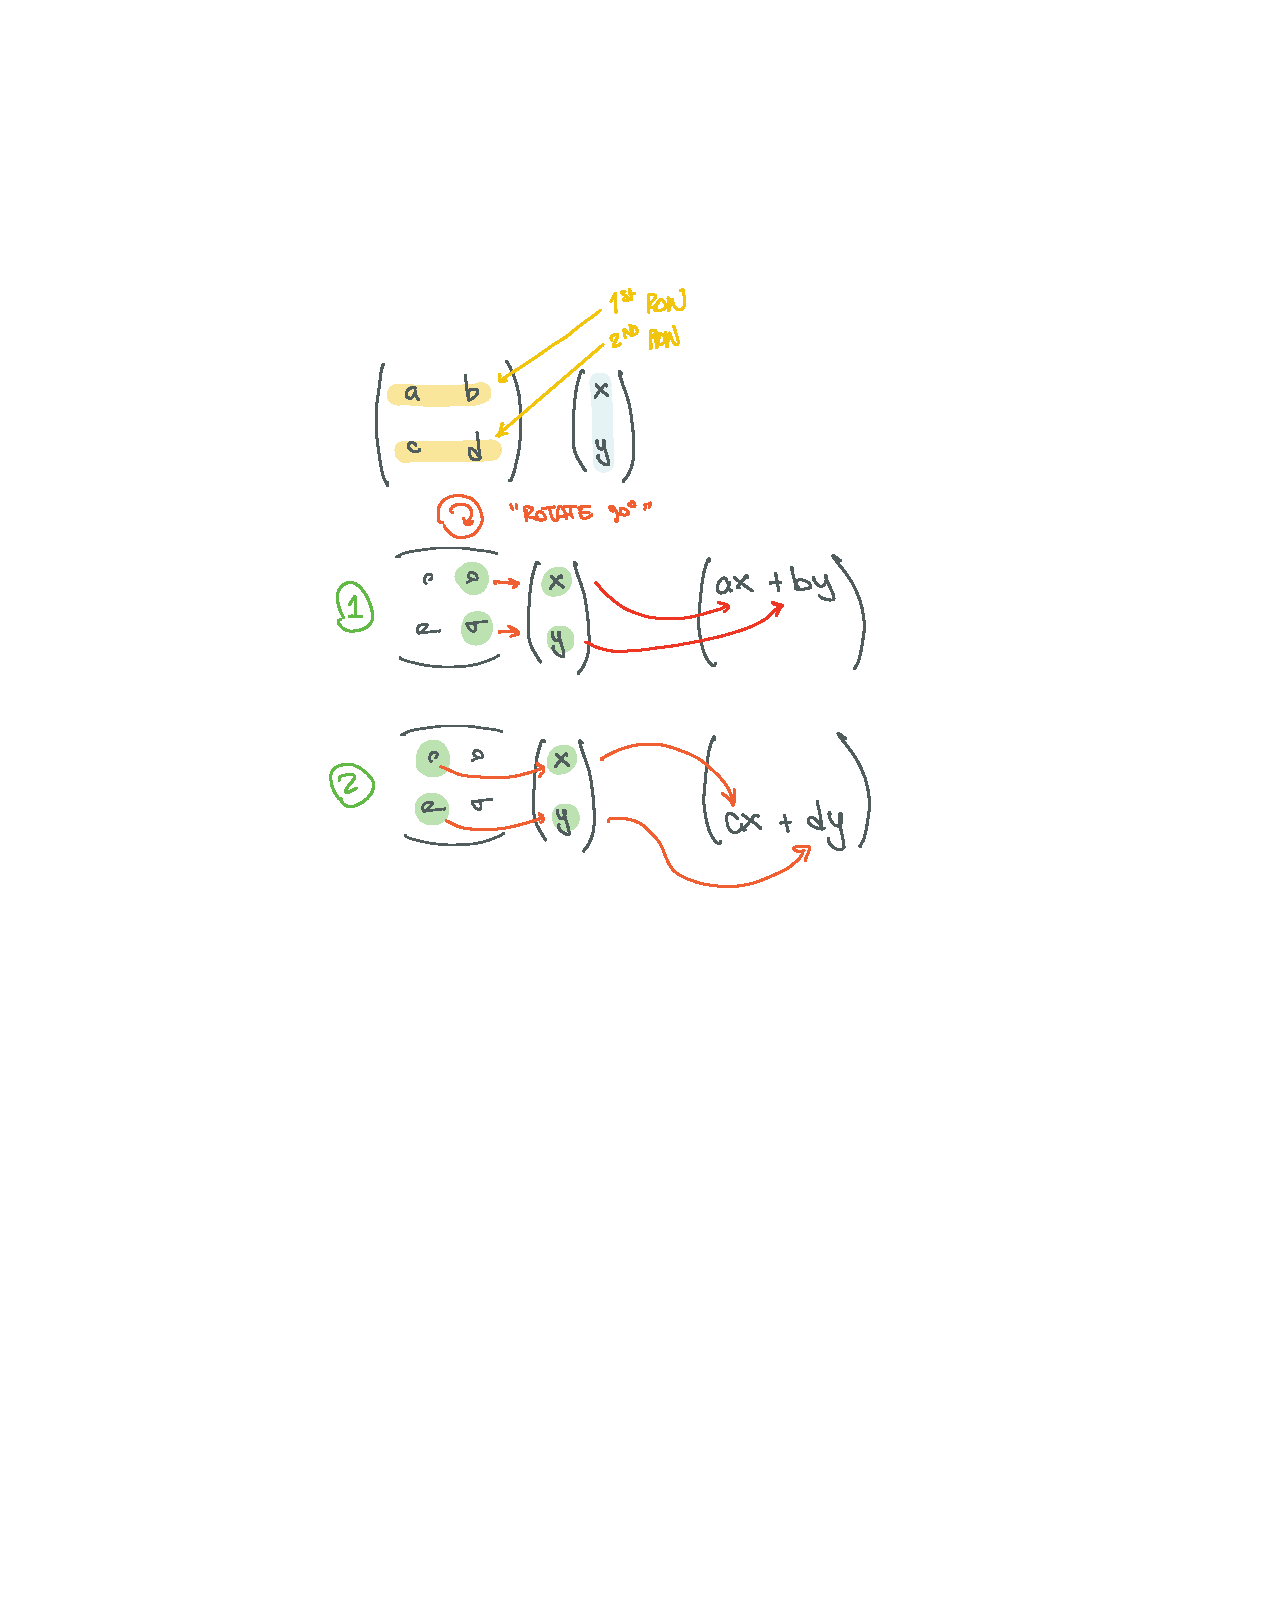
\includegraphics[width=.5\textwidth]{figures/MatrixMult_2220.pdf}
% \end{figure}
\begin{marginfigure}%[th]
    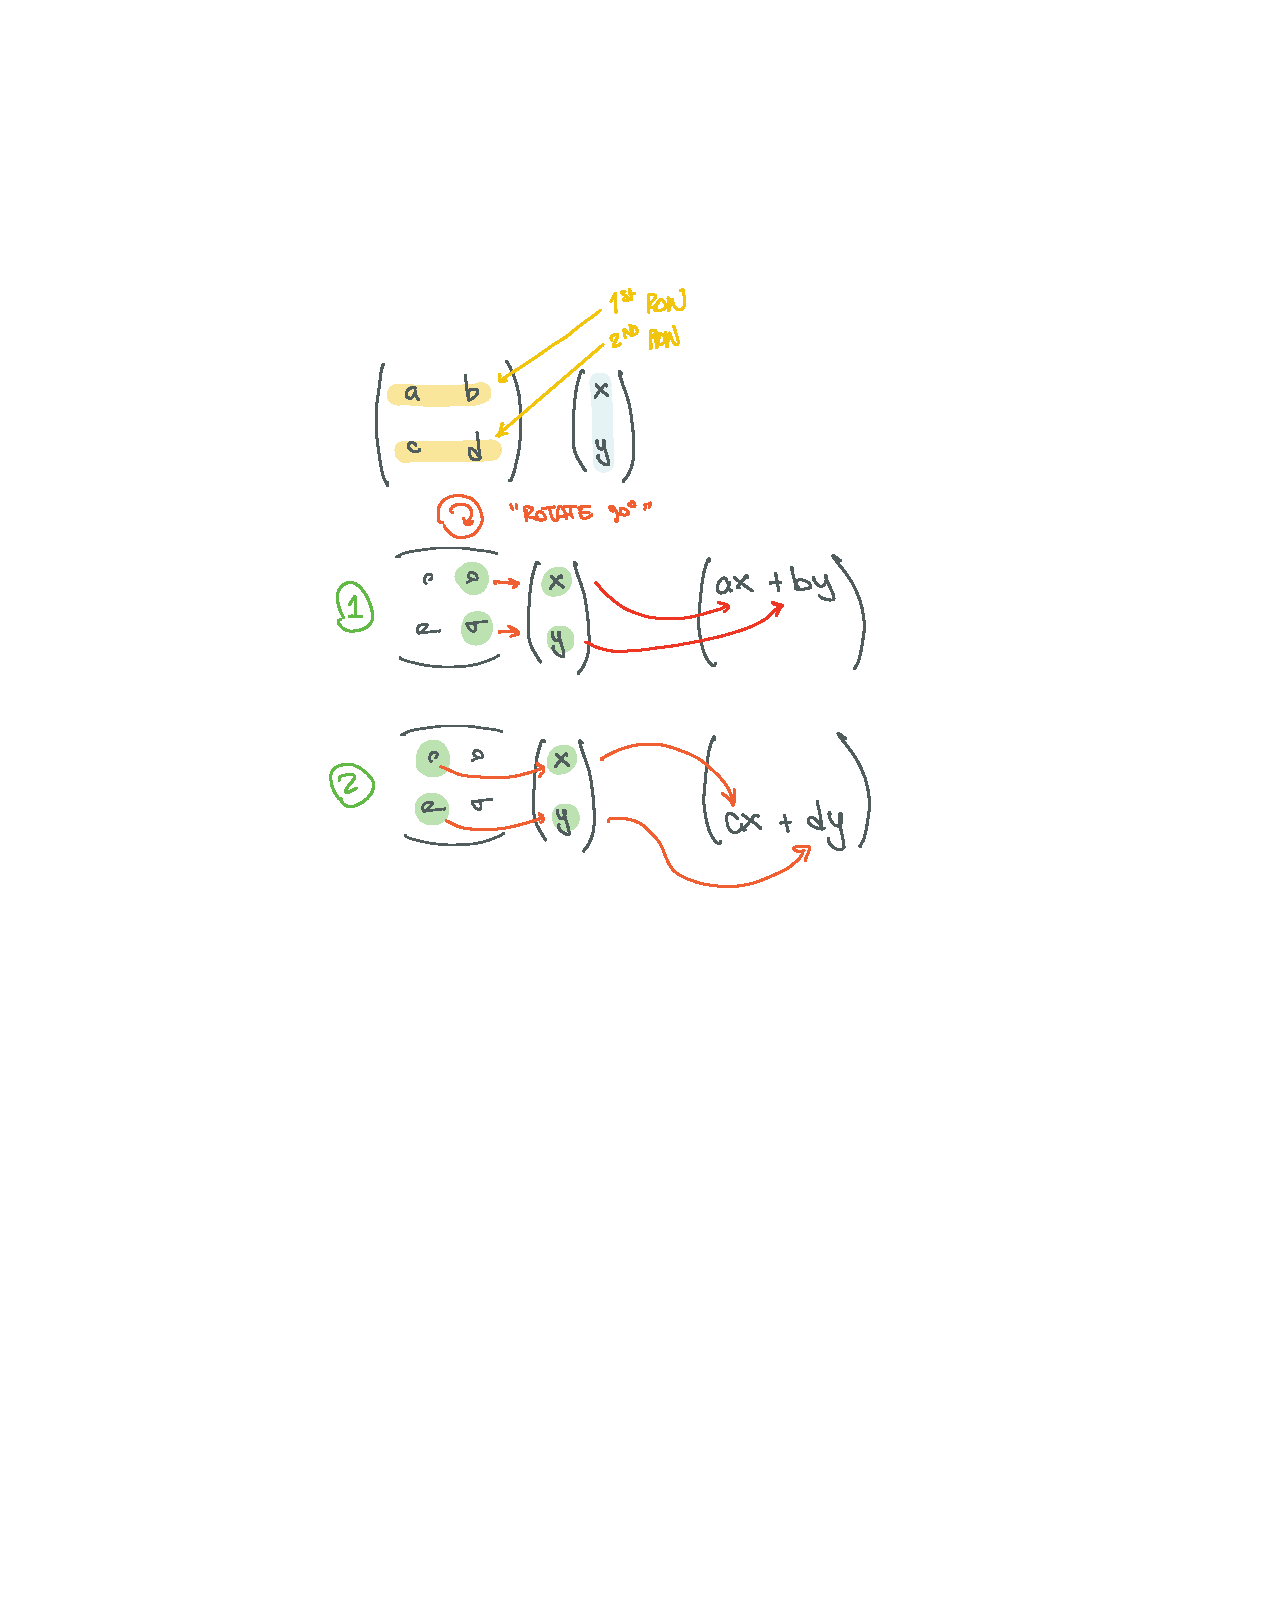
\includegraphics[width=\textwidth]{figures/MatrixMult_2220.pdf}
    \captionsetup{font={scriptsize,sf}}
    \caption{Multiplying a vector by a matrix.}
    \label{fig:matrix:mult:2220}
\end{marginfigure}
It is clunky to say the rule in words, but it goes something like this: 
\begin{enumerate}
    \item The components in the \emph{first} row of the matrix combine with the components of the column of the vector to give the \emph{first} component of $M\vec{v}$. To enact this visually,  highlight the \emph{first} row and rotate the array of numbers in $M$ clockwise by 90 degrees. The components of $M$-tipped over that are the same height as the corresponding components of $\vec{v}$ are multiplied and each product is summed together. This sum is the \emph{first} component of $M\vec{v}$.
    \item The components in the \emph{second} row of the matrix combine with the components of the column of the vector to give the \emph{second} component of $M\vec{v}$. To enact this visually,  highlight the \emph{second} row and rotate the array of numbers in $M$ clockwise by 90 degrees. The highlighted components of $M$-tipped over that are the same height as the corresponding components of $\vec{v}$ are multiplied and each product is summed together. This sum is the \emph{second} component of $M\vec{v}$.
\end{enumerate}
If you are working with three-component vectors, then there is a third step where the word `second' is replaced by `third.' 

There are other kinds of objects called row vectors. These look like vectors but they have been tipped over counter-clockwise by 90 degrees:
\begin{align}
    \row{w} = \begin{pmatrix}
        a & b
    \end{pmatrix} \ .
\end{align}
We can use this same `tip over and multiply same-height components' visualization to multiply row vectors onto vectors. See Figure~\ref{fig:matrix:mult:0220}.
\begin{figure}[ht]
    \centering
    \captionsetup{font={scriptsize,sf}}
    \sidecaption[][-2\baselineskip]{%
        Matrix multiplication of a row vector onto a [column] vector.  
        %
        %% \label command inside the \sidecaption command
        \label{fig:matrix:mult:0220}
    }
    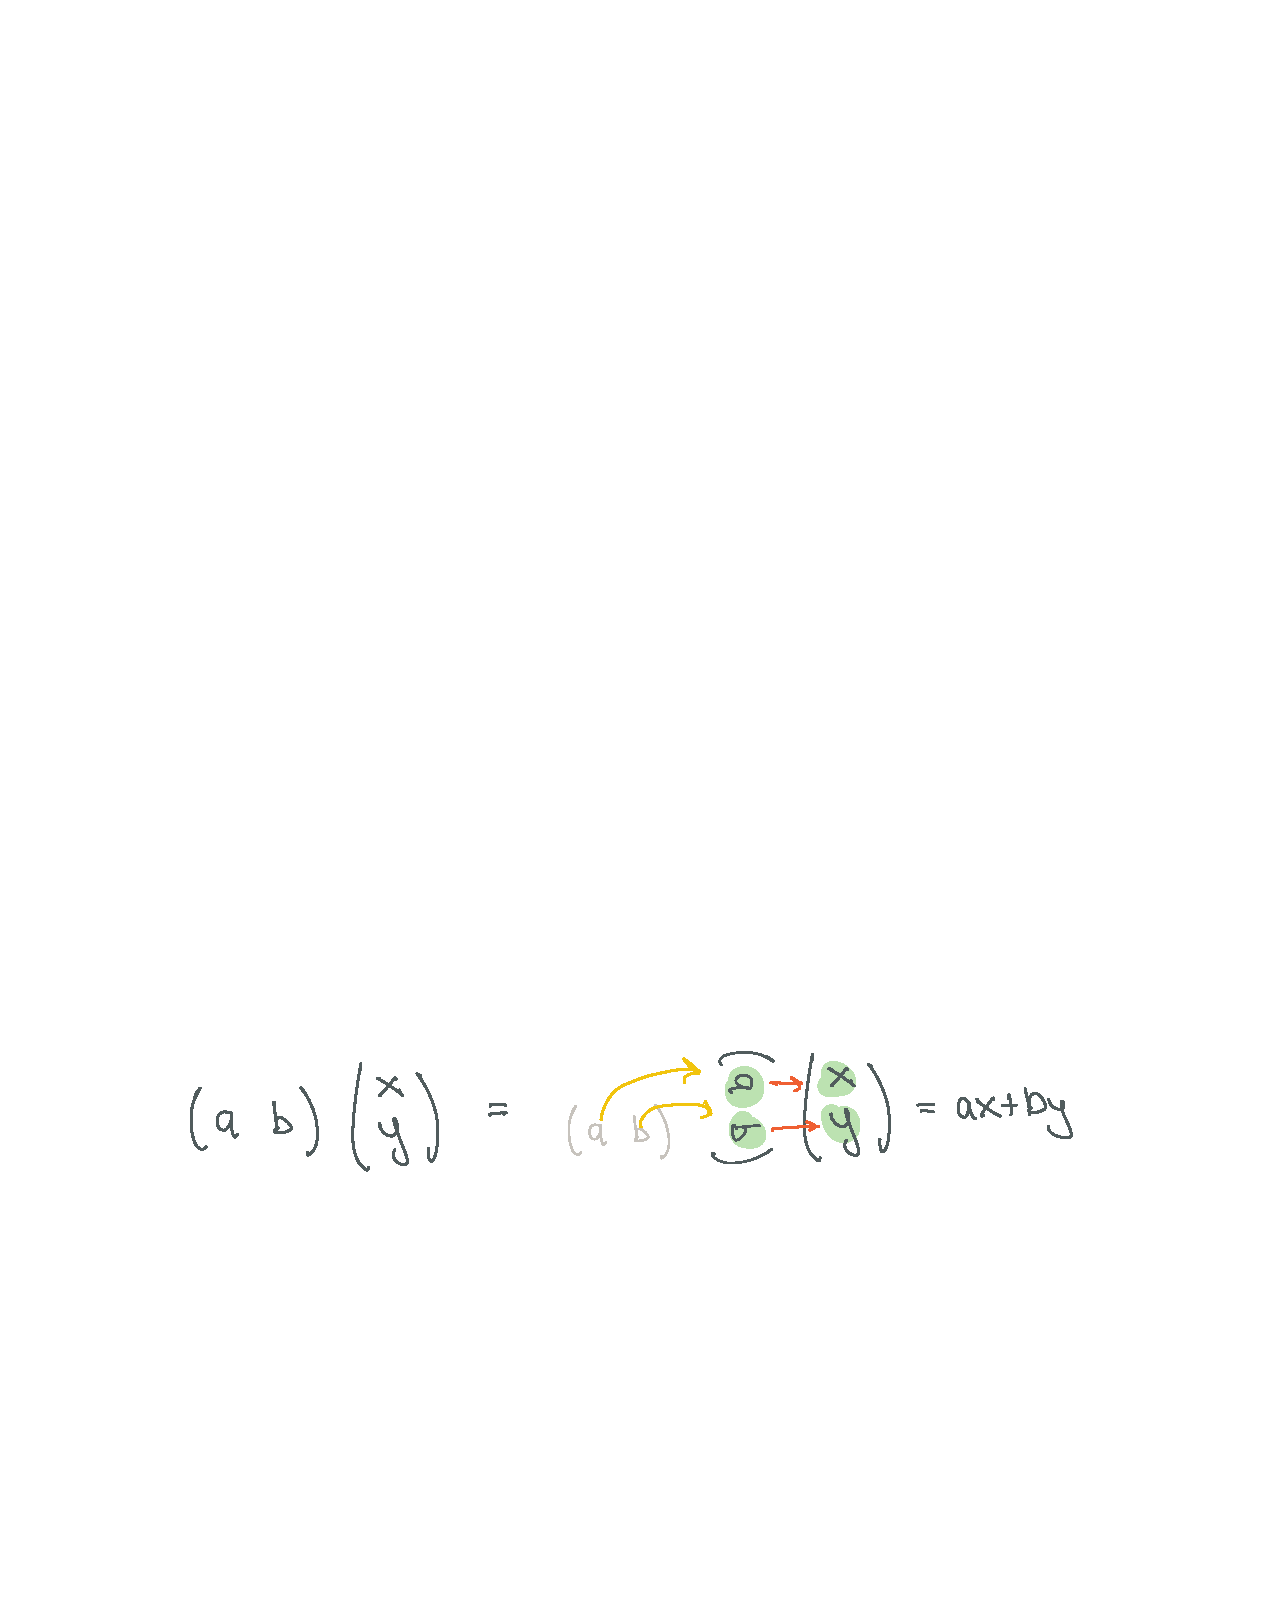
\includegraphics[width=.8\textwidth]{figures/MatrixMult_0220.pdf}
\end{figure}
Observe that the result of this multiplication is a number.
\begin{exercise}
Draw the vector
\begin{align}
    \vec{v} = \begin{pmatrix}
        1 \\ 1
    \end{pmatrix} \ .
\end{align}
Draw the vector
\begin{align}
    \begin{pmatrix}
        2 & 1 \\
        1 & 1
    \end{pmatrix}
    \begin{pmatrix}
        1 \\ 1
    \end{pmatrix} \ .
\end{align}
\end{exercise}

We can also multiply matrices with one another. The result of this is another matrix. One can construct the components of this matrix by thinking of the left matrix acting on each column of the right matrix to give the corresponding column of the matrix product. Here's how one would find the top-left component of the product of two $2\times 2$ matrices:
\begin{figure}[ht]
    \centering
    \captionsetup{font={scriptsize,sf}}
    \sidecaption[][-2\baselineskip]{%
        Multiplication of two matrices, highlighting the steps to find the top-left component of the product matrix.
        %
        %% \label command inside the \sidecaption command
        \label{fig:matrix:mult:2222a}
    }
    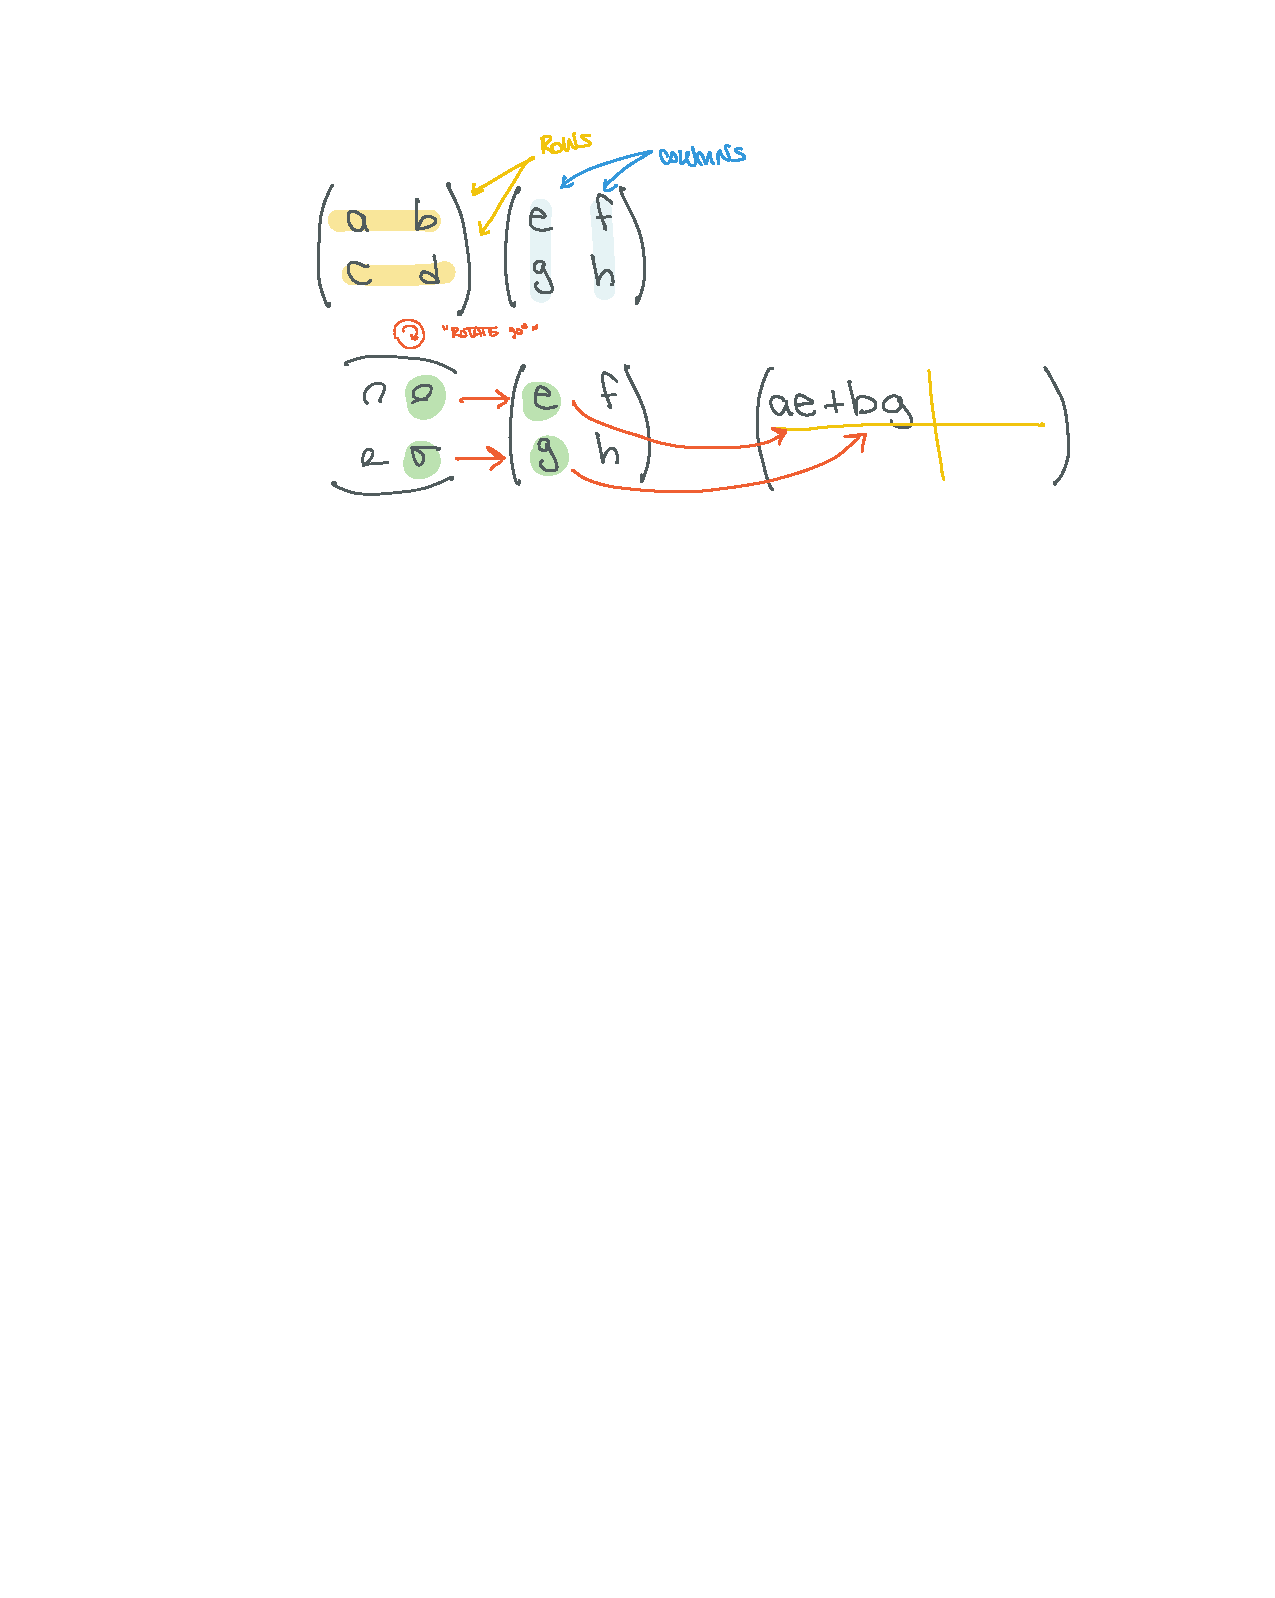
\includegraphics[width=.8\textwidth]{figures/MatrixMult_2222a.pdf}
\end{figure}
We can go on and find the top right (first row, second column) and bottom left (second row, first column) components of the product matrix, see Figure~\ref{fig:matrix:mult:2222b}.
\begin{figure}[ht]
    \centering
    \captionsetup{font={scriptsize,sf}}
    \sidecaption[][-2\baselineskip]{%
        Multiplication of two matrices, highlighting the steps to find the top right and bottom left components of the product matrix.
        %
        %% \label command inside the \sidecaption command
        \label{fig:matrix:mult:2222b}
    }
    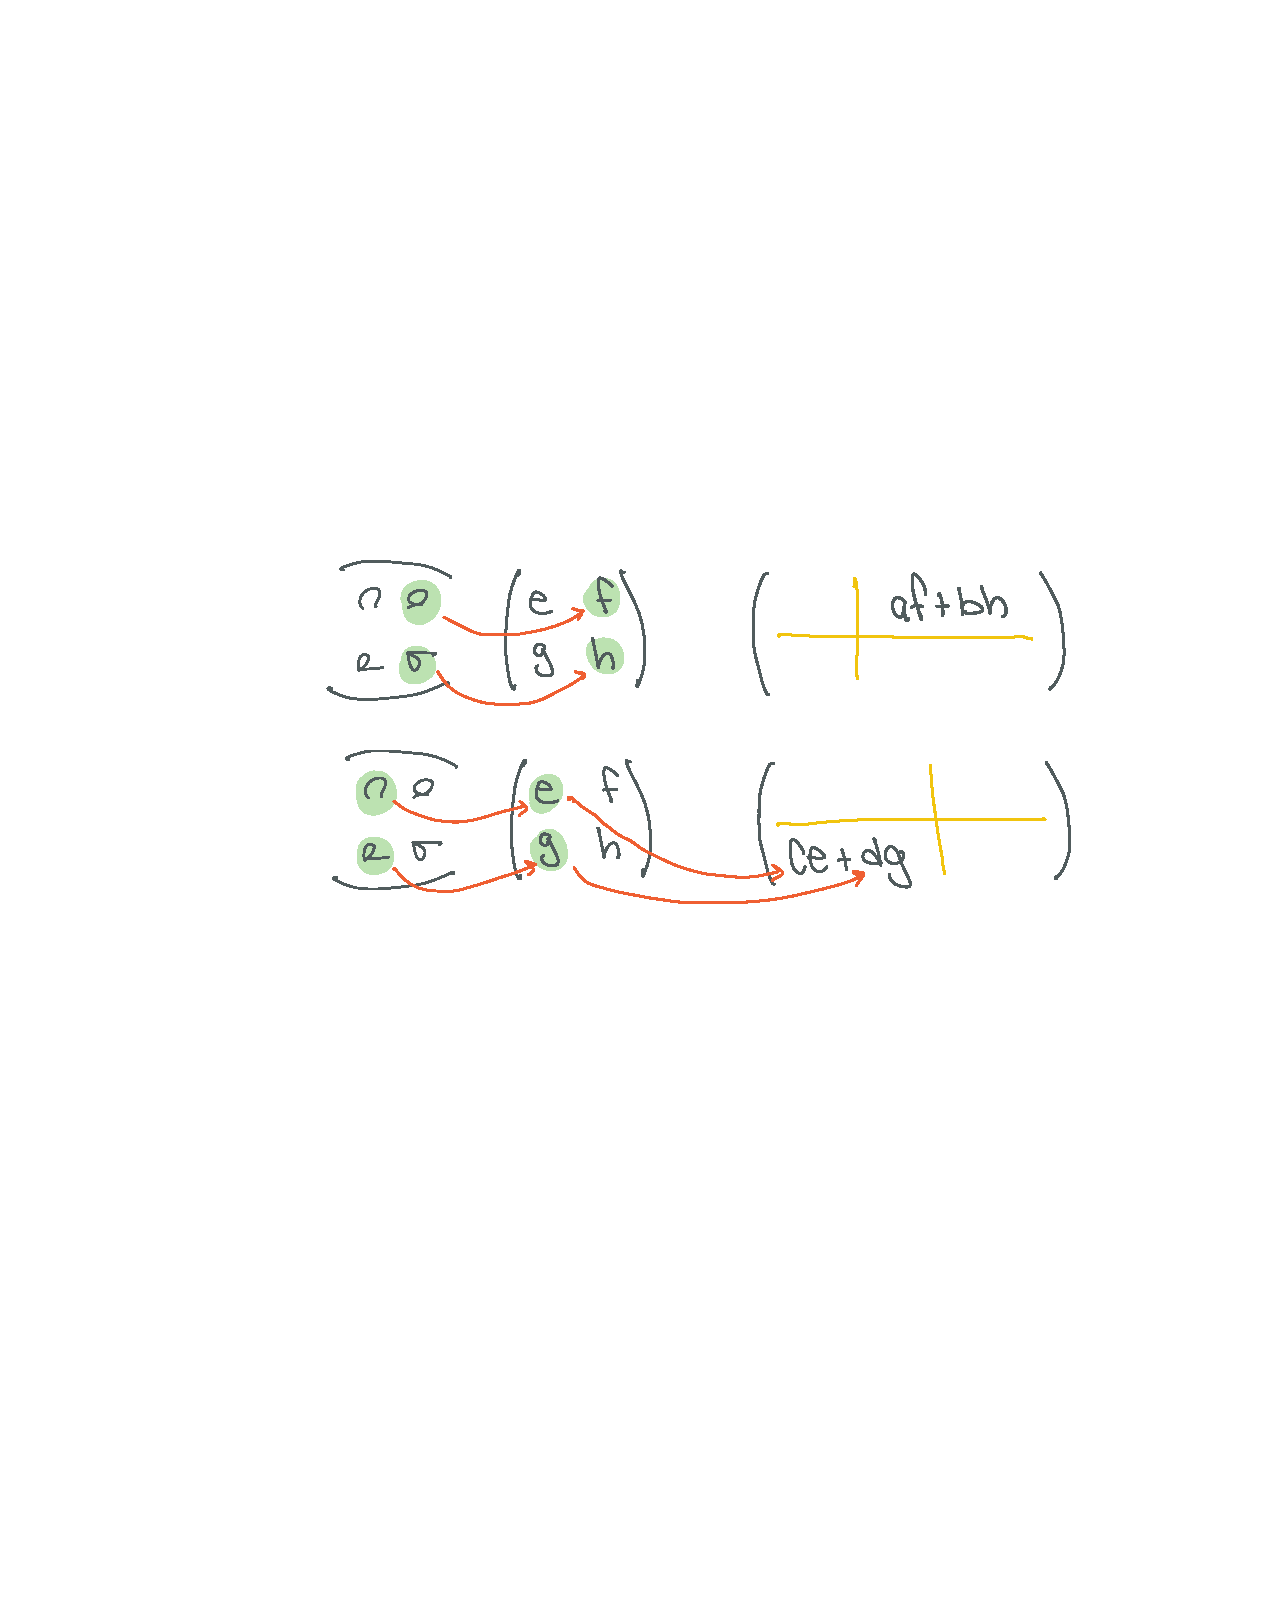
\includegraphics[width=.8\textwidth]{figures/MatrixMult_2222b.pdf}
\end{figure}
\begin{exercise}
Show that the product of two $2\times 2$ matrices $MN$ is different from the product in the opposite order, $NM$. We say that matrix multiplication is not commutative.  
\end{exercise}
\begin{exercise}
Show that
\begin{align}
\begin{pmatrix}
    2 & 1 \\
    1 & 1 
\end{pmatrix}
\begin{pmatrix}
    1 & -1 \\
    -1 & 2 
\end{pmatrix}
=
\begin{pmatrix}
    1 & 0 \\
    0 & 1
\end{pmatrix} \ .
\end{align}
The matrix on the right-hand side is called the \textbf{identity matrix}, $\one$, because when it acts on a vector it leaves the vector unchanged. We say that the two matrices on the left-hand side are \textbf{inverses}. Show further that if two matrices are inverses, $M$ and $M\inv$, then the order of the multiplication does not matter: $MM\inv M\inv M = \one$.
\end{exercise}

One can further generalize this to non-square matrices---that is, matrices with a different number of rows than columns. Those matrices will not be of direct use in this course. However, the rules of matrix multiplication follow.
\begin{exercise}
Show that you can use the matrix multiplication rules multiply a $2\times 3$ matrix onto a $3\times 2$ matrix, where our notation is $(\textnormal{number of rows})\times(\textnormal{number of columns})$.
\end{exercise}
\begin{exercise}
Show that you \emph{cannot} multiply a $2\times 3$ matrix onto a $2 \times 3$ matrix. 
\end{exercise}
\begin{exercise}
Suppose you want to multiply an $n\times m$ matrix onto a $k \times \ell$ matrix.. What are the conditions on the numbers $n, m, k, \ell$ for this to make sense using the matrix multiplication rule?
\end{exercise}



The rules for matrix multiplication also introduces the notion of a matrix inverse. Given a matrix $M$, the inverse of the matrix $M\inv$ `undoes' whatever the matrix does. It is also true that $M$ `undoes' whatever $M\inv$ does. In this sense $(M\inv)\inv = M$. The defining relation is
\begin{align}
    M M\inv = M\inv M = \one \ ,
    \label{eq:matrix:invers:multiplcation:notation}
\end{align}
where $\one$ is the identity matrix that is zero except for ones along the diagonal.\sidenote{When $\one$ acts on a vector it returns the same vector: $\one \vec{v} = \vec{v}$.}
\begin{exercise}\label{ex:matrix:inversino:the:hard:way}
Let us assign values to $M$ and $M\inv$ in the $2\times 2$ case:
\begin{align}
M &=
    \begin{pmatrix}
    a & b \\
    c & d    
    \end{pmatrix}
    &
M\inv &=
    \begin{pmatrix}
    x & y \\
    z & w    
    \end{pmatrix} \ .
\end{align}
Write out the \emph{four} conditions that we get from $MM\inv = \one$. \textsc{Partial answer}: one of the conditions is
\begin{align}
    ax + bz = 1 \ .
\end{align}
If you know each of the components of $M$, then you have four equations for four unknowns. This system of equations may have a solution.
\end{exercise}
\begin{exercise}
Using the system of equations above, prove the usual identity for $2\times 2$ invertible matrices:
\begin{align}
    M\inv = \frac{1}{ad-bc}
    \begin{pmatrix}
    \pp d & -b \\
    -c & \pp a    
    \end{pmatrix} \ .
\end{align}
\end{exercise}
All of this assumes that the inverse is well defined, which is not always the case. For example, if either a row or a column of $M$ is all zeros---the matrix will not be invertible. This is because the matrix \emph{projects out} information and there is no way to recover that information.



This notion of matrix multiplication is helpful and perhaps something you may have learned in earlier stages of your education. It is still the way I do many calculations. \emph{However}, the rules in this section are a \emph{shortcut} for a much richer mathematical structure. It is this mathematical structure that we want to reveal because it shows us how seemingly different mathematical structures in physics are actually rooted in the same underlying language. As such, many of the notions in this chapter may be ideas that you must first \emph{unlearn} in order to \emph{relearn} how they are outputs of the richer structure.\sidenote{When I teach this class there are often a few students who are apologetic for not having taken a formal linear algebra class. I have noticed that those students sometimes do much better in the course because they have fewer preconceptions to unlearn.}


\section{Rotations}\label{sec:Euclidean:three:space:rotations}

Rotations are transformations that take vectors into other vectors. They are a specific example of what is more generally known as an \emph{isometry}---and idea that we shall refer to over and over in this course. Your intuition about rotations may align with the following observations:
\begin{itemize}
    \item Rotations preserve the magnitude of vectors.
    \item Rotations preserve the angle between vectors. 
\end{itemize}
Because both magnitude and angle are related to the dot product, you may guess that rotations have something to do with the dot product. This is correct---but we need to build up some mathematical structure before we can articulate this idea carefully. In this section, we simply whet your appetite by saying that a `working definition' of rotations in Euclidean space of any dimension is that a rotation is a matrix $R$ that satisfies
\begin{align}
    R^\trans R = \one \ ,
    \label{eq:RTR:one}
\end{align}
where the \textbf{transpose} of a matrix $R^\trans$ is what happens when you flip all the elements along the diagonal:
\begin{align}
    \begin{pmatrix}
        a & b \\
        c & d
    \end{pmatrix}^\trans \defeq
    \begin{pmatrix}
        a & c \\
        b & d
    \end{pmatrix} \ .
\end{align}
We write $\one$ to mean the unit matrix: the matrix with only ones along the diagonal. Matrices $R$ that satisfy \eqref{eq:RTR:one} are called \textbf{orthogonal}\index{orthogonal}---this is just a fancy name for rotation. 

\begin{exercise}
Show that the standard form of a rotation in two dimensions,
\begin{align}
R=
    \begin{pmatrix}
    \cos \theta & -\sin\theta \\
    \sin \theta & \pp\cos\theta      
    \end{pmatrix} \ .
    \label{eq:2D:rotation:standard}
\end{align}
satisfies \eqref{eq:RTR:one}. Using this form of rotations, show that rotations in 2-dimensional Euclidean space preserve the length of vectors and the angle between vectors. \textsc{Hint}: use $\cos^2\theta + \sin^2\theta = 1$.
\end{exercise}

\begin{subappendices}
\section{Transpose}\label{sec:transpose}
The \textbf{transpose} of a matrix is what happens when you \emph{flip all the elements along the diagonal}.\sidenote{By \emph{diagonal} we mean the elements from the top left of the matrix down to the bottom right.} Given a matrix $M$, the transpose of $M$ is $M^T$ with components
\begin{align}
    (M^\trans)\aij{i}{j} &= M\aij{j}{i} \ .
    \label{eq:transpose:components}
\end{align}
This working definition of a transpose is not \emph{quite} the most useful one---but it is the most clear to write out.

\begin{example}
The following two matrices are transposes of each other.
\begin{align}
    M &= 
    \begin{pmatrix}
        9 & -3 & 2 \\
        2 & \pp 5 & 7 \\
        1 & \pp 0 & 3
    \end{pmatrix}
    &
    M^\trans &= 
    \begin{pmatrix}
        \pp 9 & 2 & 1 \\
        -3 & 5 & 0 \\
        \pp 2 & 7 & 3
    \end{pmatrix}
    \ .
\end{align}
\end{example}

This unusual operation will turn out to be rather useful for us. I leave the following cryptic statement: while the transpose of a matrix is \emph{not} its inverse, but it does have a \emph{dual} relationship to the original matrix. Once we define a metric, we will be able to give a more rigorous definition for transpose. For now, let use take \eqref{eq:transpose:components} as the definition of something we can do to matrices. We tackle this properly when we define the adjoint in Section~\ref{sec:adjoint}.


\section{Trace}

The \textbf{trace} of a matrix $M$ is simply the sum of its diagonal components:
\begin{align}
    \Tr M = M\aij{i}{i} = M\aij{1}{1} + M\aij{2}{2} + \cdots \ .
\end{align}
It is not obviously meaningful from the perspective of $M$ being a linear transformation. However, it ends up being useful as as a mechanical procedure that one can do to matrices. The reason for this is something we will see soon: the trace of a matrix is unchanged under rotations. 

\section{Determinant}
\label{sec:determinants:easy}


Here's another seemingly strange operation that you can do on a matrix. The determinant of a $2\times 2$ matrix is defined to be
\begin{align}
    \det M \equiv M\aij11 M\aij12 - M\aij12 M\aij21 \ .
\end{align}
Weird, right? Determinants for higher-dimensional square matrices can be defined recursively by taking specific linear combinations of sub-matrices. There are silly rules for this. There are fancy words for the sub-matrices (minors) and the appropriate sign for summing together those determinants (cofactors). Look, it's a mess. You should be able to calculate the determinant of a general $2\times 2$ matrix because it's easy. In case of national crisis, you should be able to calculate the determinant of a general $3\times 3$ matrix after consulting a reference to double check the signs.\sidenote{That reference will not be these notes.} However, at this stage we will not make a big deal about determinants. I think engineering classes make a big deal about determinants because they can help with solving systems of linear equations using matrices---but \emph{that's not the kind of linear algebra we're doing in physics}.

\begin{example}\label{eg:determinant:of:diagonal}
The determinant of a diagonal matrix is simply the product of each of its diagonal elements. 
\end{example}

In Chapter~\ref{ch:determinant} we take time to define the determinant properly.\sidenote{We are skipping all pretense of taking the determinant anything bigger than a $2\times 2$ matrix by hand. There are computers for that. Instead, let us figure out how to use the determinant.} 

\section{Cross product}

The cross product is an incredibly strange operation. It takes two vectors and returns another vector. Not only that, the \emph{order of the input vectors} matters. $\vec{v}\times\vec{w} = -\vec{w}\times\vec{v}$. The length of the cross product of two vectors is somehow related to the area of the parallelogram formed out of the two vectors. You have seen the cross product in your introductory physics courses: it shows up in the definition of angular momentum, the force law for a magnetic field, and the expression for the magnetic field from a vector potential. You would think that the cross product is a big part of our story. 

It is not.

The reason is that the cross product only exists in three dimensions. There is a structure that generalizes the cross product, but we first need to build up the mathematical machinery to use it. 

\section{The odd history of the vector}

I have find the history of mathematics strangely alien. As practicing physicists, we learn to \emph{use} mathematical ideas. Those who are formally inclined may lean into how these ideas are defined and generalized. But the question of ``how was it that humans came to define these ideas'' is rarely something we talk about.\sidenote{In contrast, there are plenty of great recollections of the \emph{need} to invent quantum mechanics or relativity. What was the \emph{need} to invent a vector? As American physics Nobel laureate Steven Weinberg would advise young colleagues, it is always worth it to learn the history of one's discipline.}

It should not be surprising that the history of vectors is intimately tied to physics. It may be a little more surprising that this history is also intimately connected to the history of calculus---here we wave our hands at the usual hagiographic stories of Newton and Leibniz that we like to tell in our field. I found this a \emph{little} surprising because I always thought of calculus as ``more sophisticated'' (and hence developed more recently) than vectors. What I found most surprising is that the concept of a vector is closely tied to complex analysis---a field that we do not often associate with vectorial objects---and at least one that I used to think was ``more sophisticated'' than calculus. We can point to the connection using Euler's identity:
\begin{align}
    \E^{\I\theta}  = \cos\theta + \I \sin\theta \ .
\end{align}
When we draw this, we represent $\E^{\I \theta}$ as a unit length arrow on the Cartesian plane. We say that $\cos\theta$ is the component along the $\hat x$-axis and $\sin\theta$ is the component along the $\hat y$-axis. We have drawn a two-dimensional vector. The arithmetic of complex numbers then maps onto the arithmetic of vectors. In my education, I was taught that ``of course'' this is how complex numbers and vectors work---what else would they do?

The history goes deeper. You may notice that complex numbers are different from vectors because we have a rule for multiplying complex numbers, but we do not have a rule for multiplying two-component vectors.\sidenote{``What about the cross product?'' There is no cross product for two-component vectors. There is a time to talk about the cross product---but for a large portion of this course, we do \emph{not} talk about the cross product.} If we look more carefully at the multiplication of complex numbers, we recognize that something about complex multiplication encodes rotation in the two dimensional plane. Specifically:
\begin{align}
    \E^{I\theta} \E^{I\varphi} = \E^{I(\theta+\varphi)} 
    = \cos(\theta+\varphi) + \I \sin(\theta+\varphi) \ .
\end{align}
In a more sophisticated language, we say that $\I$ \emph{generates} rotations in two dimensions. For a good portion of the 1800s, physicists sought a mathematical language to describe rotations in three dimensions. This is what William Rowan Hamilton\sidenote{Namesake of the Hamiltonian $\hat H$ and Hamiltonian mechanics, but otherwise unrelated to Alexander Hamilton of American history... \href{https://youtu.be/SZXHoWwBcDc}{youtu.be/SZXHoWwBcDc}} had been grappling with when he developed the theory of \textbf{quaternions}\index{quaternions}: an extension of complex numbers that included \emph{three} complex directions $i$, $j$, and $k$. These had the property that $i^2 = j^2 = k^2 = ijk = -1$. Unlike the relation of $\I$ to real numbers, the three distinct complex directions satisfy \emph{anticommutation} relations: $ij = -ji$. There is a moment when attentive physics students learn about quaternions and realize that they behave just like the generators of rotations acting on the spin-1/2 representation.\sidenote{Forgive me for jumping off into jargon here. As Gen-Z'ers say, \emph{if you know, you know}---but if you do not know, then the details are immaterial in this section.} All this is to say that one realizes that if Hamilton's $i$, $j$, and $k$ are actually the \textbf{Pauli matrices}\index{Pauli matrices} and if multiplication between Pauli matrices is mapped onto the commutator of those matrices, then one precisely realizes the properties of quaternions. The surprise here is that a generalization of complex numbers should have something to do with the simplest quantum mechanical system: the rotations of a spin-1/2 particle. My point here is that historically one should \emph{not} be so surprised. Ordinary complex numbers already encoded a \emph{representation}\sidenote{The word `representation' is also mathematical jargon, but we may take the colloquial meaning. A poetic definition is that a representation of an idea is related to the idea the same way shadows are related to people in Plato's allegory of the cave.} of rotations in two dimensions. This historical observation is central to the mathematical treatment of general symmetries, called \textbf{group theory}\index{group theory} and---more specifically---\textbf{representation theory}.\sidenote{The specific brand of representation theory is the representation of continuous groups, or the representation of so-called Lie algebras.}

William Rowen Hamilton imagined quaternions as a framework to describe how objects transform in three dimensions. He sought a mathematical framework to represent physical quantities that had magnitude and direction, where the direction can be acted upon by rotations. His realization that quaternions offer such a framework led him to famously scratch the quaternionic algebra into the Broom Bridge. This is the reason why some treatments of algebra---often in engineering courses for reasons I do not understand---use $i$, $j$, and $k$ to indicate the $\hat x$, $\hat y$, and $\hat z$ directions. These days, we do not talk about $i$, $j$, and $k$ as quaternions---Hamilton's invention largely comes off as a roadside curiosity on the highway of one's physics education. There is, however, more to this curiosity. The anticommutation relations of quaternions give a geometric interpretation to vector multiplication related to finding areas, volumes, and hyper-volumes formed by (hyper-)parallelograms\sidenote{A hyper-parallelogram is a parallelogram in more than two dimensions. The mathematical name for this is a parellelpiped.} of vectors. This is called \textbf{geometric algebra}\footnote{For an excellent summary in 30 minutes: \url{https://youtu.be/1cRFfYQYGxE}} and has recently had a quiet resurgence in mathematical physics. There is a reasonable argument for systematically incorporating geometric algebra into the physics curriculum~\autocite{Doran:2007tqa}\footnote{There is also room for lively counter-arguments: \url{https://alexkritchevsky.com/2024/02/28/geometric-algebra.html}}. The mathematically inclined may want to explore these topics further,\autocite{chisolm2012geometricalgebra,chappell2016geometricalgebranaturalrepresentation,brechet2022rotationsclassicalmechanicsusing,lundholm2009cliffordalgebrageometricalgebra,brechet2022electrodynamicsgeometricalgebra,Lasenby:2019gmi,almeida2005geometricalgebraparticledynamics} where applications even span contemporary applications in machine learning and robotics.\autocite{hitzer2013introductioncliffordsgeometricalgebra} For more on the history of the concept of vectors, I highly recommend \emph{Vector} by Robyn Arianrhod, see Fig.~\ref{fig:arianrhod}.
\begin{marginfigure}%[th]
    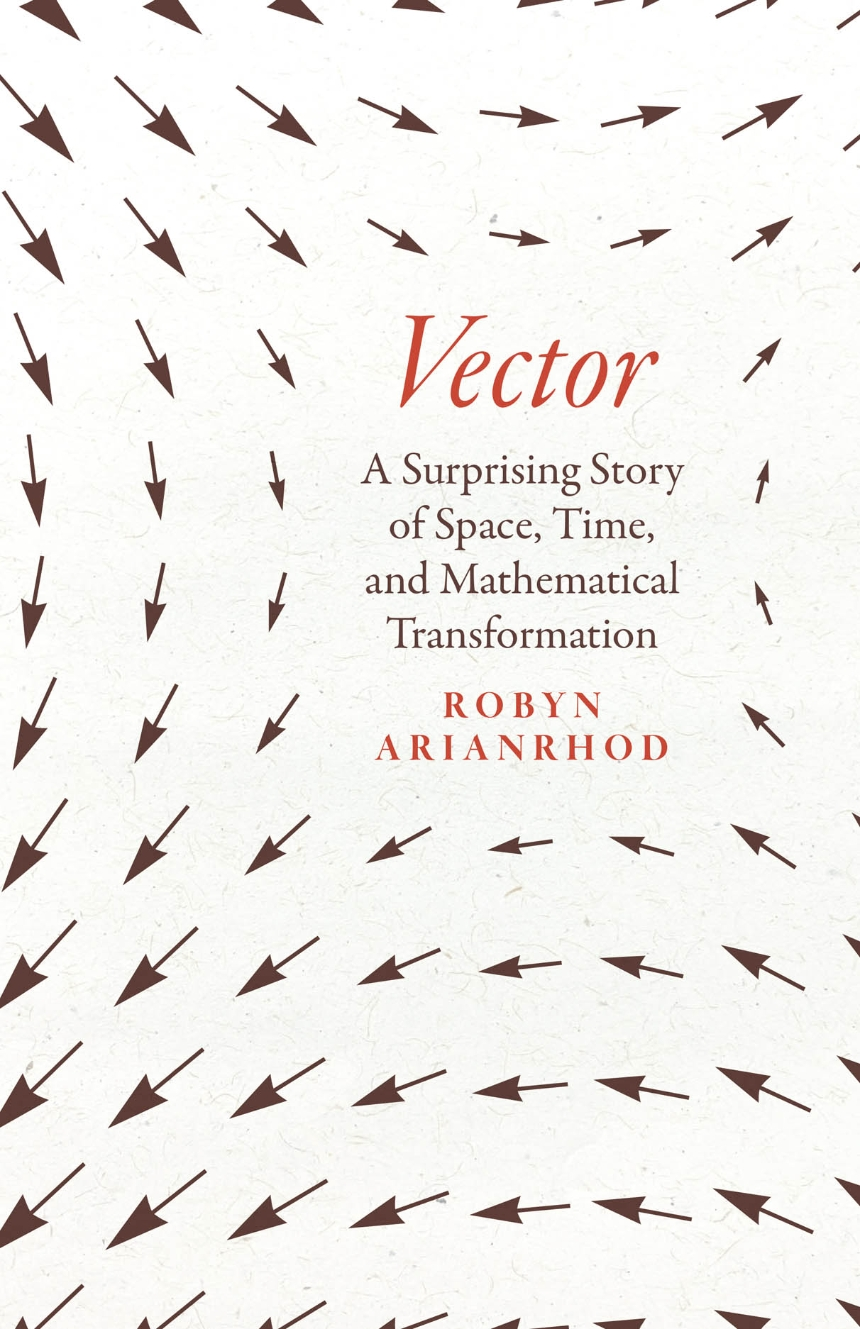
\includegraphics[width=.8\textwidth]{figures/VectorArianrhod.jpg}
    \captionsetup{font={scriptsize,sf}}
    \caption{\cite{arianrhod2024vector}}
    \label{fig:arianrhod}
\end{marginfigure}


% \autocite{ogawa2009housekeeper}

\end{subappendices}



\chapter{Indexology}\label{ch:indexology}
\begin{quote}
... should not prevent us from avoiding purely formal calculations where a \emph{debauchery of indices} hides an often simple geometrical reality. -- E.~Cartan, \emph{Lecons sur la Geometrie des Espaces de Riemann}\sidenote{From Spivak, \emph{A Comprehensive Introduction to Differential Geometry}, volume 2.}\footnote{\cite{spivak1975comprehensive}; see also \url{spivak1975comprehensive}}
\end{quote} % cite https://hsm.stackexchange.com/questions/3320/the-debauch-of-indices-translation-request

In this chapter we introduce the rules for index notation. Please accept them for now as a necessary complication---there is nothing deep here, only a set of conventions and one useful shorthand (summation convention). The utility of these may not be obvious until we start to see how this is used and where it comes from.

\section{Tensors and index notation}
\label{sec:index:notation}

In this course we make a \emph{big deal} about the height of indices. This means the index does more than  `index' a number in an array. In fact, in physics there are objects that carry multiple indices with different heights. Here is one such example, the Riemann tensor in general relativity: $R^a_{\phantom{a}bcd}$. This object has four indices. The first one, $^a$ is raised, and the following three, $_{bcd}$ are lowered. There needs to be an unambiguous ordering of the indices: it is clear that the index $b$ is the \emph{second} index, the index $c$ is the \emph{third} index, and so forth. So it would be disastrous to write $R^a_{bcd}$ because now we cannot tell whether the upper index $^a$ or the lower index $_b$ is the \emph{first} index. This is demonstrated in Figure~\ref{fig:Riemann:tensor:for:indices}.
\begin{marginfigure}%[th]
    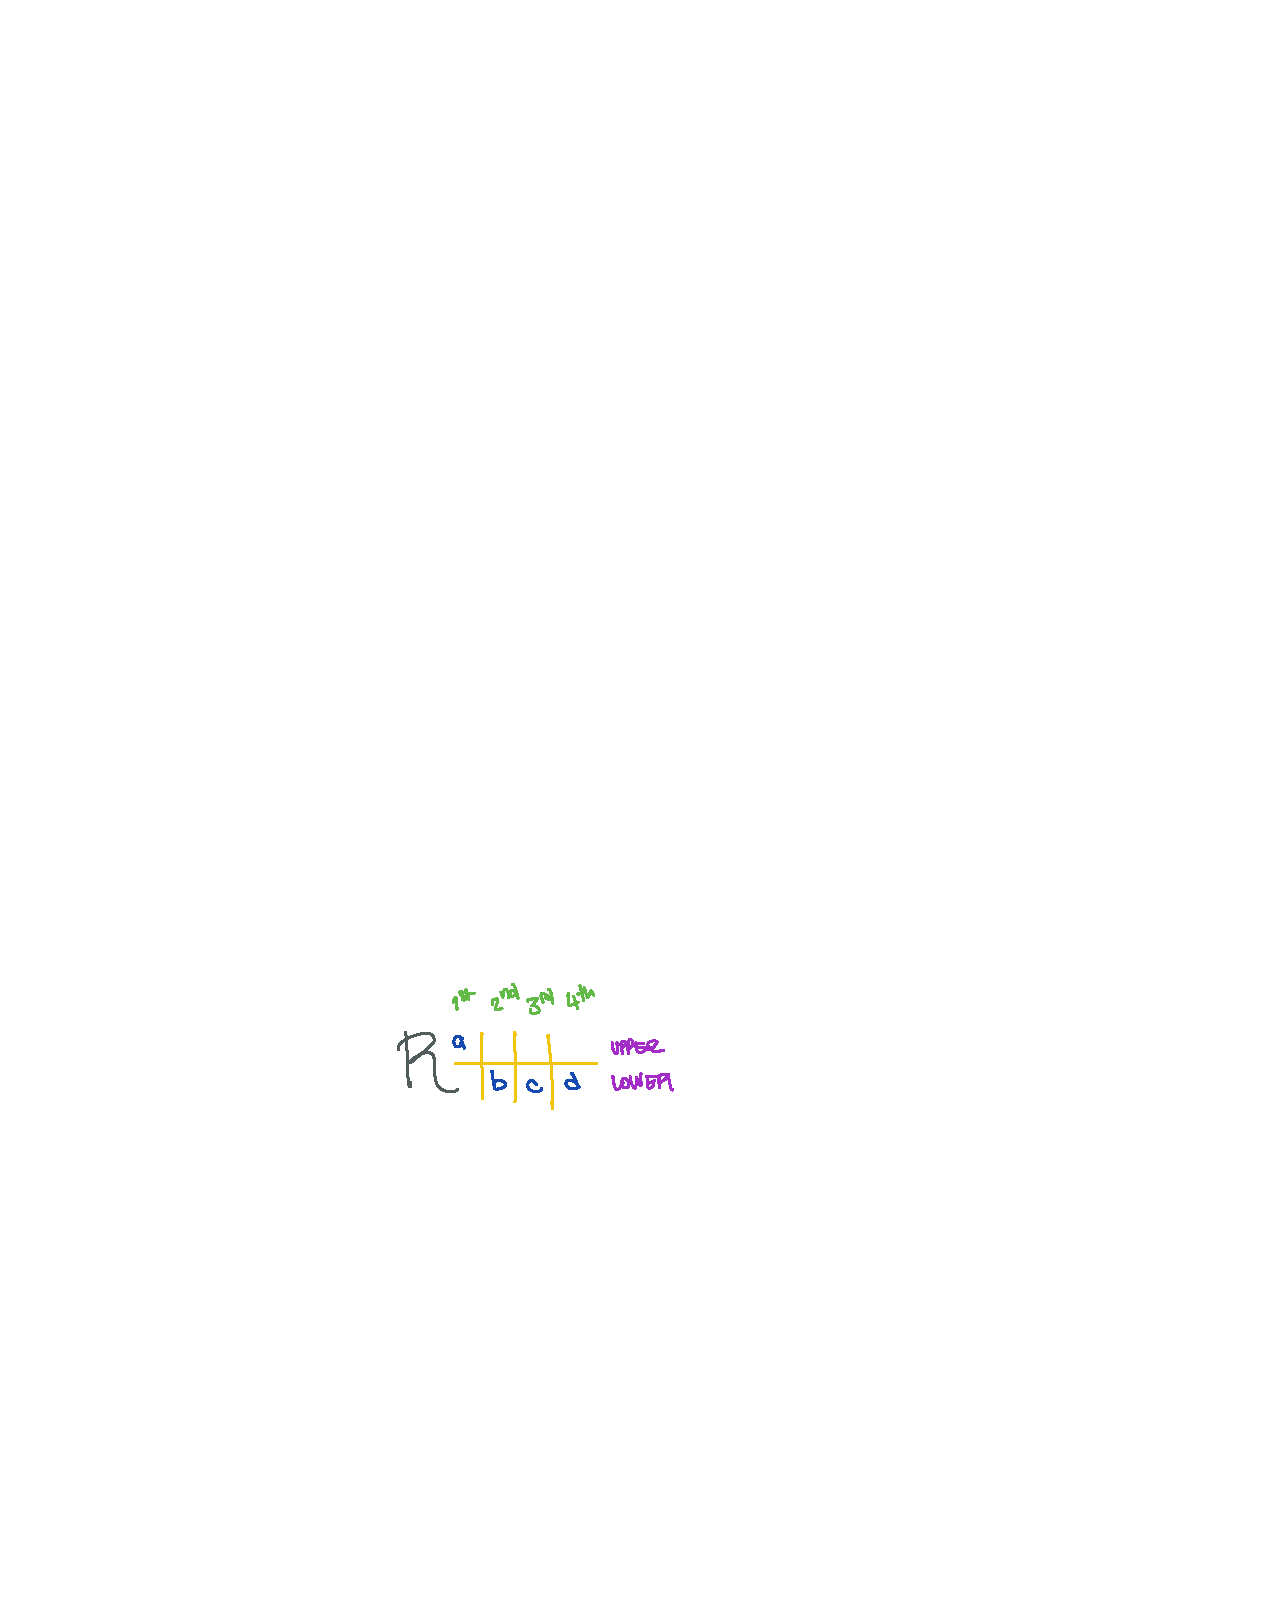
\includegraphics[width=.8\textwidth]{figures/Rabcd_eg.pdf}
    \captionsetup{font={scriptsize,sf}}
    \caption{The Riemann tensor showing the significance of the ordering and height of its indices.}
    \label{fig:Riemann:tensor:for:indices}
\end{marginfigure}

So let us get to the elephant in the room. To a physicist, a \textbf{tensor}\index{tensor} is an object that has indices. In this sense, vectors and matrices are both types of tensors. They can have any number of indices, but the indices have a well defined order and a well defined height (raised or lowered). In general, the following two objects are different:
\begin{align}
    M\aij{i}{j} &&\text{and} && M_i^{\phantom{i}j} \,
\end{align}
even though both are two-index objects whose first index is $i$ and second index is $j$. 

Why do we make such a big deal about indices and their heights? The difference between a tensor and an array of numbers is that tensors have specific \emph{transformation rules} under symmetries. The symmetry that you are most familiar with is rotational symmetry. From your first-year coursework, you are familiar with how useful it is to rotate to coordinates where a problem is simpler. The most common example of this is calculating the moment of inertia of a rotating body. There we had an object called the \emph{moment of inertia tensor}\sidenote{The transformation rules of this tensor are precisely why it is not called a ``moment of inertia \emph{matrix}.'' Though you may be hard pressed to find an honest textbook that explains this.\footnotemark}\footnotetext{See e.g.\,\url{https://hepweb.ucsd.edu/ph110b/110b_notes/node24.html}} One of the groan-inducing exercises in mechanics is to find the rotation in which the moment of inertia tensor of a rotating body is diagonal.

Here is what we need to know for now:
\begin{enumerate}
    \item In physics, tensors are objects with indices. These are arrays of numbers so that a particular choice of indices corresponds to a number in the tensor. The order of the indices matters.
    \item But there is more: whether an index is upper or lower indicates how that part of the tensor transforms under a symmetry transformation such a rotations. 
\end{enumerate}
At this point, you may have several questions, such as these:
\begin{enumerate}
    \item How exactly does a tensor transform under symmetries?
    \item What are examples of other symmetries?
    \item How should I visualize an object with more than two indices? (Yes, you can think of a three-index object as a hypercube arrays of numbers. No, I do not know of a good way to visualize upper versus lower indices on this array.)
\end{enumerate}
We shall answer these as we build up the machinery below. Just take this section as a request to believe that there may be method to this madness.

\section{The treachery of indices}
\label{sec:treachery:of:indices:vi:is:not:a:vector}

There is something that physicists do that tend to drive mathematicians crazy: we write a generic \emph{component of a vector} and refer to it as if it were the vector itself. It is a fairly harmless peccadillo:\sidenote{There are times when you can get into trouble if you drink your own Kool Aid, so to speak. The reason is that the \emph{component} $v^i$ is simply a number, whereas $\vec{v}$ is a vector. Some manipulations are only allowed for numbers and not vectors, and you should be clear that you mean `the component $v^i$' if you are treating it like a number, and not `the \emph{vector} whose components are $v^i$.' %See Example~\ref{eg:moving:coefficients:around}.
} if I say
\begin{quote}
the vector $v^i$
\end{quote}
then it is not hard to guess that I mean
\begin{quote}
the vector $\vec{v}$ which has components that I label $v^i$.
\end{quote}
If you ever meet a mathematician who gives you a hard time about this, you can wave your hands and refer to something called \emph{abstract index notation}, developed by Roger Penrose.\footnote{\url{https://math.stackexchange.com/questions/455478/}} To the best of my understanding, this is simply a formal way to justify the way physicists talk about indices. 

The reason why we have this culture is that this index notation ends up being so damn convenient. In addition to vectors, we will have other objects that have indices: dual vectors, matrices, and tensors. When we write everything in with indices, we can ``see'' properties of these objects that are not obvious without the indices. Specifically, we can see \emph{how an object transforms under symmetries}. In this course, we will focus on \emph{rotations} of vectors and their generalizations. 

Whenever I think about whether $v^i$ means the vector $\vec{v}$ or the $i^\textnormal{th}$ component of that vector, I am reminded of Magritte's ``The Treachery of Images,'' Figure~\ref{fig:Magritte}\footnote{From \url{https://en.wikipedia.org/wiki/The_Treachery_of_Images}, please refer to this page for fair use justification.}
\begin{marginfigure}%[th]
    
\includegraphics[width=.8\textwidth]{figures/MagrittePipe.jpg}
    \captionsetup{font={scriptsize,sf}}
    \caption{``La Trahison des Images'' (``The Treachery of Images'') by Ren\'e Magritte. Owned by \tacro{LACMA}, reproduced here under fair use.}
    \label{fig:Magritte}
\end{marginfigure}
In this image, Magritte shows a painting of a pipe and then writes ``this is not a pipe.'' The implied message is that it is a \emph{painting} of a pipe that we may use to express the \emph{idea} of a pipe.


\section{Summation Convention}
\label{sec:summation}


There is another reason why indices are convenient: they allow us to use \textbf{summation convention}.\sidenote{Sometimes called Einstein summation convention in deference to its progenitor. With respect to Einstein, we simply write \emph{summation convention} because it's not like the dude is underappreciated in popular culture.} This is a notational shortcut that introduces upper and lower indices to convey sums. Consider, for example, the ``matrix multiplication'' of a row vector $\row{w}$ on a column vector $\vec{v}$. Nevermind the formal definition of ``row vector'' as opposed to ``column vector.'' Let us write it out in components where it is obvious for $\RR ^3$:
\begin{wide}
\begin{align}
    \row{w}
    &=
    \begin{pmatrix}
        w_1 & w_2 & w_3
    \end{pmatrix}
    &
    \vec{v}
    &=
    \begin{pmatrix}
        v^1 \\ v^2 \\ v^3
    \end{pmatrix}
    &
    \row{w}\vec{v}
    &= w_1v^1 + w_2v^2+w_3v^3 \ .
\end{align}
\end{wide}
On the far right we have used the matrix multiplication rules in Section~\ref{sec:matrix:multiplication}.
% The final expression is familiar, right? It follows the usual rules of matrix multiplication for a ``matrix'' that happens to be one row and three columns; 
We review this rule in Fig.~\ref{fig:row:col:mult}, labeling the components with upper and lower indices as appropriate.
% %% FIGURE SNIPPIT
\begin{marginfigure}[.01em]%[tb]
    \centering
    \captionsetup{font={scriptsize,sf}}
    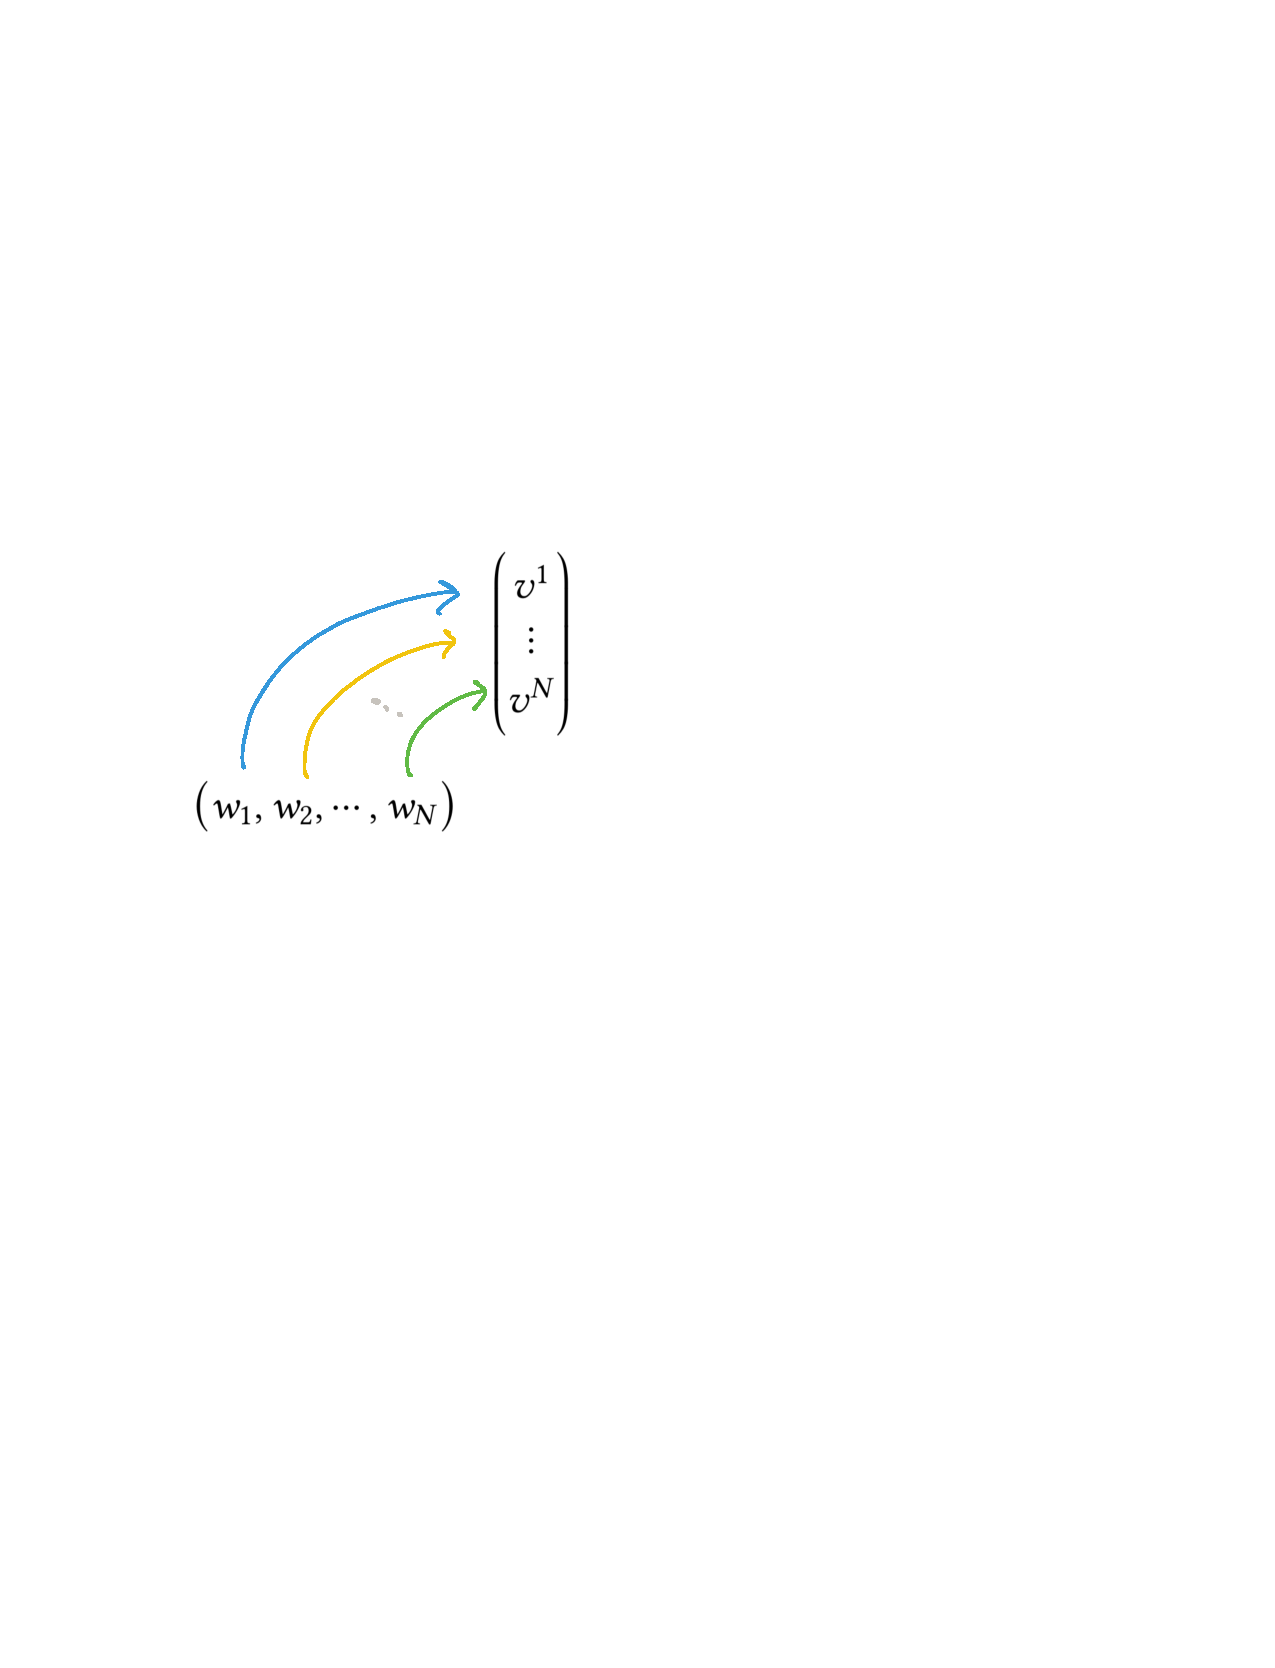
\includegraphics[width=.8\textwidth]{figures/rowcolmult.pdf}
    \caption{The `matrix multiplication rule' for acting with a row vector on a column vector.}
    \label{fig:row:col:mult}
\end{marginfigure}
Notice that we choose to write the components of $\row{w}$ with lower indices---this is the convention. Row vectors have indices written as subscripts while column vectors have indices written as superscripts. There is no mathematics here, just a choice of notation. The result of the multiplication is simply a number, which we can write as a sum:
\begin{align}
    \row{w}\vec{v}
    &= \sum_{i=1}^3 w_iv^i
    \equiv w_iv^i \ .
    \label{eq:row:w:on:vec:v}
\end{align}
On the right-hand side we have \emph{defined} the summation convention:
\begin{newrule}[Summation convention]
Whenever there is exactly one upper index and exactly one lower index with the same letter, we should understand that there is a sum over that index over all of its allowed values. We call pairs of repeated indices where one is upper and one is lower \textbf{contracted indices}\index{contract}.
\end{newrule}



The value $w_iv^i$ is simply a number. It is not a vector. It does not have any ``vectorial'' (tensorial) structure. It is not an element of the vector space $\RR ^3$. It does not transform under rotations. It is \emph{just a number}. In other words, $w_iv^i$ behaves like an object with \emph{no indices}. Contracted indices ``cancel each other out.''

This is significant because we will see that indices tell us how objects transform. Evidently, column vectors and row vectors transform differently since one has an upper index and one has a lower index. Further, when we contract the two indices, we end up with something with no indices: a number that does not transform at all. This may seem like notational overkill---trust me, it is worth building this notation now. We will use it over and over.



\begin{example}
Matrices $M$ have the following index structure: $M\aij{i}{j}$. There is a first index and a second index---the order matters. The first index is upper, and the second index is lower. Matrix multiplication boils down to a contraction of indices:
\begin{align}
    (M\vec{v})^i = M\aij{i}{j}v^j \ .
    \label{eq:matrix:mult:ith:comp}
\end{align}
Let us read this equation carefully. First, $M\vec{v}$ is a vector. The $i^\text{th}$ component of this vector is $(M\vec{v})^i$. How is this related to the components of $M$ and $\vec{v}$? The right-hand side tells us that we simply take the sum:
\begin{align}
    M\aij{i}{j}v^j = 
    M\aij{i}{1}v^1 + M\aij{i}{2}v^2  + M\aij{i}{3}v^3 \ .
\end{align}
\end{example}

\begin{figure}[tb]
    \centering
    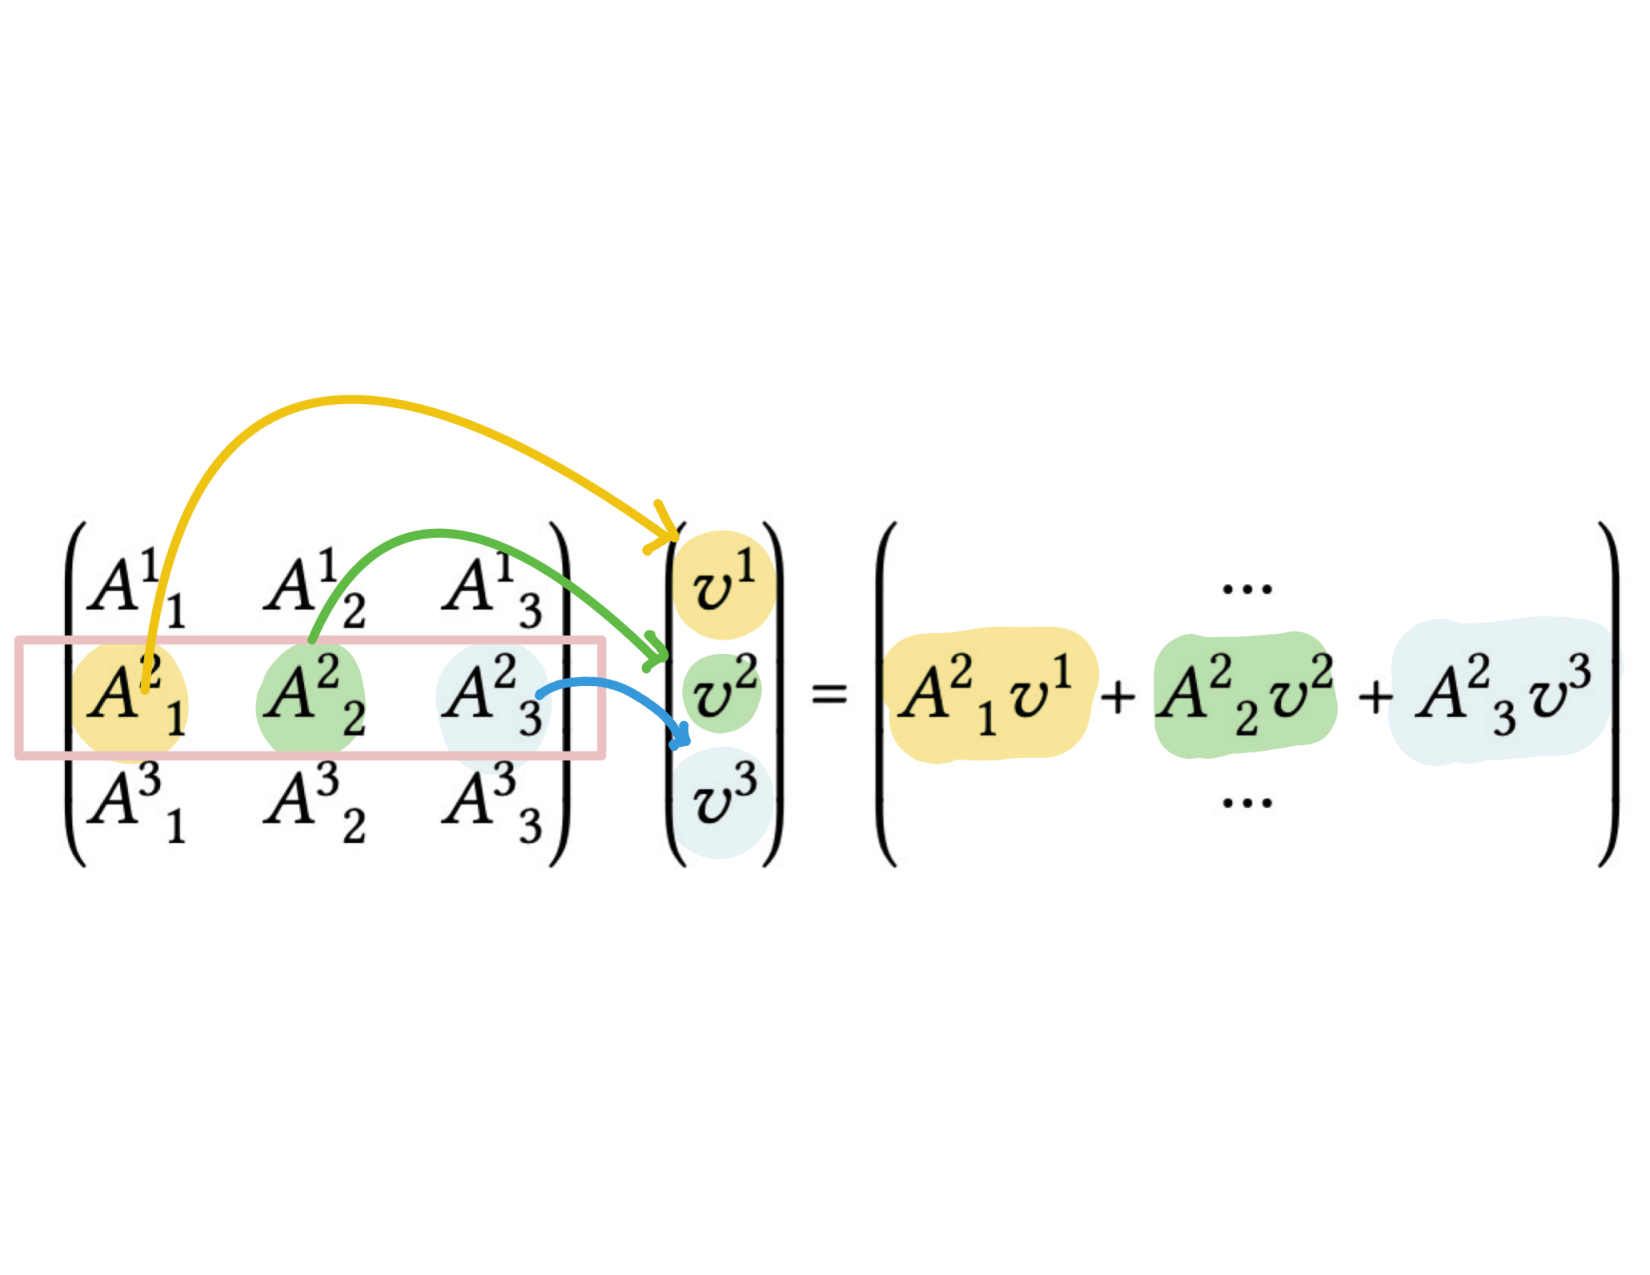
\includegraphics[width=.5\textwidth]{figures/matrixmultiplication.pdf}
    \caption{The `matrix multiplication' rule for $A\vec{v} = \vec{v}'$. We show that the second element of $\vec{v}'$ is a sum of terms, where each term is a multiplication of the $j^\text{th}$ column of the $2^\text{nd}$ row of $A$ by the $j^\text{th}$ row of $\vec{v}$.}
    \label{fig:matrix:col:mult}
\end{figure}

\begin{example}
From the above example, you can then excuse the glib statement: ``the \emph{vector} $M\aij{i}{j}v^j$.'' As we explained above, $M\aij{i}{j}v^j$ is not a vector, but a component of a vector. However, the point is that even though there are three indices, two of them are contracted so the object effectively only has one upper index. This is the index structure of a vector. This matches the usual matrix multiplication rule shown in Fig.~\ref{fig:matrix:col:mult}.
\end{example}

\begin{exercise}
Consider the following vector, row vector, and matrix:
\begin{align}
    \vec{v} &=
    \begin{pmatrix}
     1 \\ 2 \\ 3   
    \end{pmatrix}
    &
    \row{w} &=
    \begin{pmatrix}
        4&5&6
    \end{pmatrix}
    &
    M&=
    \begin{pmatrix}
        1 & 2 & 3 \\
        4 & 5 & 6 \\
        7 & 8 & 9
    \end{pmatrix} \ .
\end{align}
These have index structure $v^i$, $w_i$, and $M\aij{i}{j}$ respectively. Note that the first index of a matrix is the row and the second is the column, thus $M\aij{1}{2} = 2$ while $M\aij{2}{1} = 4$. Calculate the following: $(wM)_2$, $(Mv)^1$, $(MM)\aij{1}{2}$. Here $MM$ is understood to be the square of the matrix $M$, $(M^2)\aij{i}{j} = M\aij{i}{k}M\aij{k}{j}$.
\end{exercise}

\begin{example}\label{eg:moving:coefficients:around}
It should be clear that
\begin{align}
    w_i M\aij{i}{j} = 
    w_1 M\aij{1}{j} + w_2 M\aij{2}{j} + w_3 M\aij{3}{j}
    = 
    M\aij{1}{j}w_1  + M\aij{2}{j}w_2 + M\aij{2}{j}w_2
    =
    M\aij{i}{j}w_i \ .
\end{align}
After all, each of the components $w_i$ and $M\aij{i}{j}$ are simply numbers. However: even though $w_i M\aij{i}{j} = M\aij{i}{j}w_i$, it is \emph{completely incorrect} to say $\row{w}M = M\row{w}$. This is because $\row{w}$ and $M$ are \emph{tensorial} (vector-y) objects. The order of their `multiplication' matters. You can see this from the matrix notation.
\begin{align}
    \row{w}M &= 
    \begin{pmatrix}
        4&5&6
    \end{pmatrix}
    \begin{pmatrix}
        1 & 2 & 3 \\
        4 & 5 & 6 \\
        7 & 8 & 9
    \end{pmatrix}
    &
    M\row{w} &=
    \begin{pmatrix}
        1 & 2 & 3 \\
        4 & 5 & 6 \\
        7 & 8 & 9
    \end{pmatrix}
    \begin{pmatrix}
        4&5&6
    \end{pmatrix} \ .
\end{align}
The first multiplication gives a row vector, as you expect since $(wM)_j$ has one lower index. The second multiplication does not even make sense. What we see is that expressions like $w_i M\aij{i}{j} = M\aij{i}{j}w_i$ are valid as long as you are only talking about the components. The glib ``physicist slang'' of replacing a component by its vector/matrix/tensor can get you into trouble if you have moved components around in a way that is only allowed for numbers, but not vectory-things.
\end{example}

Since the language is now becoming cumbersome, let us define the word \textbf{tensorial} to mean an object with indices. This will replace the phrase ``vectory'' in our notes.




One neat thing about this is that our convention for contracting indices makes it clear that $(Mv)^i$ is a component of a vector: it has one upper index. Similarly, you may recall that the multiplication of matrices $M$ and $N$ proceeds as follows:
\begin{align}
 (MN)\aij{i}{j} = M\aij{i}{k}N\aij{k}{j} \ .
 \label{eq:matrix:matrix:multiplication}    
\end{align}
\begin{exercise}
Confirm that \eqref{eq:matrix:matrix:multiplication} holds for $2\times 2$ matrices.
\end{exercise}
On the right-hand side of \eqref{eq:matrix:matrix:multiplication}, we have one pair of contracted indices $_k^{\phantom{k}k}$, one upper index $^i$, and one lower index $_j$. We thus deduce that this object is a matrix: it has one upper and one lower index. Indeed, the product of two matrices is also a matrix. Our indices and contraction rules tell us what kinds of objects we can produce by contracting indices between them. 

\begin{example}
You may also contract indices within an object. For example, because a matrix has one upper and one lower index, you may contract them together. This is called the \textbf{trace}\index{trace}, $\Tr M = M\aij{i}{i}$. Alternatively, you may remember the trace as the sum of all diagonal elements in a matrix. This corresponds to 
\begin{align}
    M\aij{1}{1} + M\aij{2}{2} + \cdots = M\aij{i}{i} \ ,
\end{align}
where we simply recognize that the summation convention is a shortcut for the `sum of all diagonal elements' rule. The significance of the trace is that as an object with no indices---they're both contracted---it is a pure number. Under rotations, the trace does not change. If you measure something that is the trace of a tensor, it does not matter what coordinate system you are in---you measure the same thing.
\end{example}


\chapter{Vectors, Row Vectors, Matrices}
\label{ch:vectors:row:matrices:in:indices}

We begin a systematic study tensorial objects. Let us re-state some of the results from earlier chapters.\sidenote{The cost of stating things systematically is repetition. However, often there is pedagogical value to deliberate repetition.} In fact, we start by stating the \emph{sloppy} (technically incorrect) understanding---everything as indexed objects---and then we start to define the underlying mathematical machinery `under the hood.'

It may seem that we are inventing sophisticated machinery in order to justify the simple index-based rules in Chapter~\ref{ch:indexology}. Perhaps that is in fact what we are doing. There is good reason for this: it is the ``underlying sophisticated machinery'' that we can generalize to different physical systems.

\begin{example}
This approach of \emph{learn how to use it then learn how it works} is a trusted pedagogical tradition. You likely learned Newtonian mechanics long before you learned Lagrangian mechanics. Newtonian mechanics taught you how to use $\vec{F} = m\vec{a}$, conservation of energy, and so forth. Lagrangian mechanics involved a lot of new machinery---variational calculus---that culminated in... what? Deriving $\vec{F}=m\vec{a}$, conservation of energy, and so forth. But in doing so, it created the framework that could be extended to both quantum mechanics\footnote{Formally through a process called geometric quantization, but less formally by identifying the role of the action in the path integral formulation of quantum mechanics.} and relativity\footnote{Where the laws of relativity are elegantly stated as action principles.}.
\end{example} 

\section{First pass: components}
\label{sec:component:notation}
% Index notation
%   Matrices as two indexed objects.

We start by leaning on our recent familiarity with index notation to introduce our primary players.

\subsection{Vectors}

A \textbf{vector}\index{vector} is an object that has one upper index,\sidenote{The notation $\simeq$ here means \emph{not quite equal but you know what I mean}, as discussed in Section~\ref{sec:treachery:of:indices:vi:is:not:a:vector}.}
\begin{align}
    \vec{v} = \ket{v} \simeq v^i \ .
\end{align}
On the left-hand sides we introduce two different notations for vectors. They also have different names: vector, column vector, contravariant vector, ket. These are all equivalent names that are used in different subfields. For each value of $i$, $v^i$ is the $i^\textnormal{th}$ component of the vector. 


\begin{newrule}[Linear combinations of vectors are vectors]\label{rule:vector:linear:combinations}
Vectors can be rescaled and added.
\begin{enumerate}
    \item You can rescale a vector $\vec{v}$ by a number, $\alpha$. This simply rescales each component by the number\footnote{The fancy mathematical name for what we are calling number is \textbf{field}. For now by `number' we mean a real number.} $\alpha$:
    \begin{align}
        \vec{v} \to \alpha\vec{v} \simeq \alpha v^i
    \end{align}
    so that the components of the vector rescaled by $\alpha$ are simply $\alpha v^i$. The result of this operation is (obviously) a vector.
    \item You can add two vectors together, $\vec{v} + \vec{w}$. The result is also a vector. The components of the combined vector are the sum of the components of each individual vector:
    \begin{align}
        (\vec{v}+\vec{w})^i = v^i + w^i \ . \label{eq:vector:addition:rulex}
    \end{align}
    You should read this to say the $i^\textnormal{th}$ component of the sum of $\vec{v}$ and $\vec{w}$ is simply the sum of the $i^\textnormal{th}$ component of $\vec{v}$ plus the $i^\textnormal{th}$ component of $\vec{w}$.
\end{enumerate}
The general combination of rescaling and adding is called a \textbf{linear combination}\index{linear combination}; for vectors $\vec{v}$ and $\vec{w}$ and numbers $\alpha$ and $\beta$
\begin{align}
    (\alpha \vec{v} + \beta\vec{w})^i = \alpha v^i + \beta w^i \ .
\end{align}
This says that the combination $(\alpha\vec{v}+\beta\vec{w})$ is a vector and its $i^\textnormal{th}$ components is the right-hand side of the above equation.
\end{newrule}

There are other formal aspects that we can (justifiably) take for granted. These include the following:
\begin{enumerate}
    \item There is a zero vector, $\vec{0}$, whose components are all zero. 
    \item Every vector has an additive inverse that is simply rescaling $\vec{v}$ by $\alpha=-1$.
    \item The order of vector addition does not matter. This is inherited from \eqref{eq:vector:addition:rulex}. \sidenote{This is somewhat subtle. On the left-hand side of \eqref{eq:vector:addition:rulex} we \emph{define} vector addition by defining each component of the sum. We do not know if the $+$ sign on the left-hand side is commutative. On the right-hand side we are using ordinary addition of numbers, which we know is commutative. Using this definition we can see that because $v^i+w^i = w^i+v^i$, it must be that $(\vec{v}+\vec{w})^i = (\vec{w}+\vec{v})^i$. Since this is true for every component, then the $+$ sign on vectors must be commutative: $\vec{v}+\vec{w}= \vec{w}+\vec{v}$.}
\end{enumerate}
% \begin{enumerate}
%     \item There is a zero vector, $\vec{0}$, whose components are all zero. 
%     \item Every vector has an additive inverse that is simply rescaling $\vec{v}$ by $\alpha=-1$.
%     \item The order of vector addition does not matter. This is inherited from \eqref{eq:vector: addition:rulex}. %\sidenote{This is somewhat subtle. On the left-hand side of \eqref{eq:vector: addition:rule} we \emph{defining} vector addition by defining each component of the sum. We do not know if the $+$ sign on the left-hand side is commutative. On the right-hand side we are using ordinary addition of numbers, which we know is commutative. Using this definition we can see that because $v^i+w^i = w^i+v^i$, it must be that $(\vec{v}+\vec{w})^i = (\vec{w}+\vec{v})^i$. Since this is true for every component, then the $+$ sign on vectors must be commutative: $\vec{v}+\vec{w}= \vec{w}+\vec{v}$.}
% \end{enumerate}




\subsection{Row Vectors}

There is another kind of vector. These are equivalently called \textbf{row vectors}\index{row vectors}, dual vectors, covariant vectors, one-forms, linear forms, linear functionals, or bras. A row vector is an object that has one lower index,
\begin{align}
    \row{w} = \bra{w} \simeq w_i \ .
\end{align}
These behave just like vectors.
\begin{newrule}[Row vectors are also vectors]
Linear combinations of row vectors are also row vectors. We may thus take Rule~\ref{rule:vector:linear:combinations} and replace all the vectors with row vectors, and all the vector components with row vector components.
\end{newrule}

At this point row vectors\sidenote{dual vectors, covectors, one-forms, bras} are pretty cheap copies of column vectors\sidenote{column vectors, contravariant vectors, kets}. They just happen to have lower indices. Indeed, row vectors are \emph{dual} to column vectors in a way that only comes through when we carefully define basis vectors.

Now that we have objects with lower indices, we can make use of our summation convention from Section~\ref{sec:summation}. Row vectors are `born' to contract column vectors:
\begin{align}
    w_i v^i = v^i w_i = w_1 v^1 + w_2 v^2 + \cdots \ .
\end{align}
This means the following:
\begin{itemize}
    \item If you have a row vector and a column vector, you can contract them to get a number.
    \item If you have a row vector, you can think of it as a function that takes in a vector and spits out a number. 
    \item If you have a column vector, you can think of it as a function that takes a row vector and spits out a number. 
\end{itemize}
Observe that the relation of a row vector to a column vector is the same as the relation of the column vector to a row vector. The two are dual to one another.

Let us be clear that the contraction of a row vector with a column vector is \emph{not} a dot product. This misconception can stem from the belief that you can take the `transpose' of a vector to tip it over. We have \emph{not yet} defined what transpose means, and where we do, it \emph{definitely} is not an operation that acts on vectors. In order to create a row vector from a column vector, one requires an additional bit of mathematical machinery called a \emph{metric}. In ordinary Euclidean space, this machine is simply the identity and so when we first learn about vectors, we can freely go between vectors and row vectors. This is \emph{not generally the case} and we would not have special relativity if it were.

\subsection{Matrices}

A \textbf{matrix}\index{matrix} is an object with two indices: the first index is raised, the second index is lowered, see Figure~\ref{fig:Mij:index:heights}.
\begin{marginfigure}%[th]
    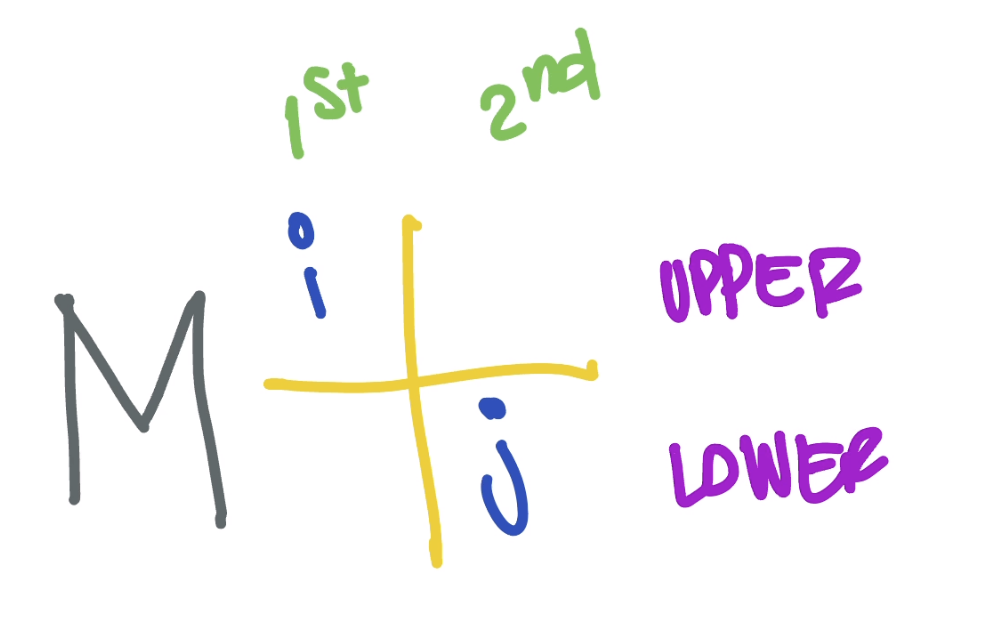
\includegraphics[width=.7\textwidth]{figures/Mij_indices.png}
    \captionsetup{font={scriptsize,sf}}
    \caption{The index placement for a matrix.}
    \label{fig:Mij:index:heights}
\end{marginfigure}
You can take linear combinations of matrices in the same way you take linear combinations of vectors, as per Rule~\ref{rule:vector:linear:combinations}. That is, given two matrices $M$ and $N$, the $ij$-component of the sum of these matrices is
\begin{align}
    (M+N)\aij{i}{j} = M\aij{i}{j} + N\aij{i}{j} \ .
\end{align}
The extension to linear combinations (including rescaling) is trivial.\sidenote{Trivial is how mathematicians say `obvious.' If this point is not obvious, take a moment to see if there is a better way to think about this.}
\begin{example}
Matrices can also be interpreted as vectors. If the index $i$ can run from $1$ to $N$, then a matrix can be understood as an $N^2$-component object. For $2\times 2$ matrices, we could write
\begin{align}
    \vec{v} = 
    \begin{pmatrix}
        v^1 & v^2 \\
        v^3 & v^4
    \end{pmatrix} \ .
\end{align}
In this way, it is a weird repackaging of a 4-component vector. You can check that you can take linear combinations of these `vectors' to form other vectors in the usual way. In this way, the matrix is a repackaging of the components of a vector. Of course, these `vectors' are \emph{completely different} from the 2-component vectors that the $2\times 2$ matrices act on. This identification is rather silly at this point. However, it plays a role in what is called representation theory: the mathematical description of symmetries.
\end{example}

The index structure of matrices means it can contract with both upper-indexed objects like vectors and lower-indexed objects like row vectors. This can happen in several ways. Suppose you have a matrix $M\aij{i}{j}$:
\begin{itemize}
    \item If you also have a row vector $w_i$ and a column vector $v^i$, then you can form a number by contracting them together in the only allowed way: $w_i M\aij{i}{j}v^j$.
    \item If you have a column vector $v^i$, then you can form another column vector by contracting them in the only allowed way: $M\aij{i}{j}v^j$. Observe that this object has one free\sidenote{Here free means uncontracted.} upper index so that it is a column vector.
    \item If you have a row vector $w^i$, then you can form another row vector by contracting them in the only allowed way: $w_iM\aij{i}{j}$. Observe that this object has one free lower index so that it is a row vector.
    \item If you only have the matrix $M\aij{i}{j}$, you can form a number by contracting its two indices, $M\aij{i}{i}$. This is called the \textbf{trace}\index{trace} of the matrix.
\end{itemize}
You can easily understand the first three contractions from your intuition using the matrix multiplication language of Section~\ref{sec:matrix:multiplication},
\begin{align}
    \row{w} M \vec{v} &= 
    \begin{pmatrix}
        w_1 & w_2
    \end{pmatrix}
    \begin{pmatrix}
        M\aij{1}{1} & M\aij{1}{2}\\
        M\aij{2}{1} & M\aij{2}{2}
    \end{pmatrix}
    \begin{pmatrix}
        v^1 \\ v^2
    \end{pmatrix}
    =  
    w_i M\aij{i}{j} v^j
    \\
    \row{w} M &= 
    \begin{pmatrix}
        w_1 & w_2
    \end{pmatrix}
    \begin{pmatrix}
        M\aij{1}{1} & M\aij{1}{2}\\
        M\aij{2}{1} & M\aij{2}{2}
    \end{pmatrix}
    =  
    \begin{pmatrix}
        w_i M\aij{i}{1} & w_i M\aij{i}{2}
    \end{pmatrix}
    \\
    M\row{v} &= 
    \begin{pmatrix}
        M\aij{1}{1} & M\aij{1}{2}\\
        M\aij{2}{1} & M\aij{2}{2}
    \end{pmatrix}
    \begin{pmatrix}
        v^1 \\ v^2
    \end{pmatrix}
    =  
    \begin{pmatrix}
        M\aij{1}{i}v^i \\ M\aij{2}{i}v^i
    \end{pmatrix} \ .
\end{align}
But here we see something powerful about the index notation: in matrix notation, it \emph{does not} make sense to act on a row vector with a matrix `from the right,'
\begin{align}
    M\row{w} = ? \ .
\end{align}
However, from an index point of view:
\begin{align}
    M\aij{i}{j}w_i = w_i M\aij{i}{j} \ .
\end{align}
This is because $M\aij{i}{j}$ is not the matrix $M$, it is a specific \emph{component} of the matrix $M$. As such, it is just a number and multiplication of numbers is commutative.\sidenote{I refer back to Section~\ref{sec:treachery:of:indices:vi:is:not:a:vector}.} Similarly,
\begin{align}
    M\aij{i}{j}v_j = v_j M\aij{i}{j} \ ,
\end{align}
and
\begin{align}
    w_i M\aij{i}{j}v_j = v_j w_i M\aij{i}{j} = v_j  M\aij{i}{j} w_i \ ,
\end{align}
and so forth. This is not `breaking' anything. In fact, our indexology rules are highlighting that it is the matrix multiplication language of Section~\ref{sec:matrix:multiplication} that is limited. 

We re-iterate once more:
\begin{newrule}[Contracted indices] The type of object (tensor) that you have after performing an contraction is determined by the leftover \emph{uncontracted} indices.
\end{newrule}
This means that the trace, $M\aij{i}{i}$ is a number because it has no free (uncontracted) indices. It also means that a matrix acting on a vector $M\aij{i}{j}v^j$ is a vector because it has one free upper index. Of course, we can also imagine other types of objects that return something different when contracting with a vector.

\paragraph{Matrix multiplication} In terms of index notation, matrix multiplication is the contraction of the upper index of one matrix with the lower index of the other. If we multiply matrices $M$ and $N$ in that order, then the $i$--$j$ component of the product is:
\begin{align}
    (MN)\aij{i}{j} =   M\aij{i}{k} N\aij{k}{j}  = N\aij{k}{j} M\aij{i}{k} \ .\label{eq:multiplication:MN:indices}
\end{align}
The second equality here is simply a statement that the product of \emph{numbers} is commutative. Explicitly for the two dimensional case:
\begin{align}
    (MN)\aij{i}{j} &= 
    M\aij{i}{1} N\aij{1}{j} + M\aij{i}{2} N\aij{2}{j}\\
    &=
    N\aij{1}{j} M\aij{i}{1}  + N\aij{2}{j} M\aij{i}{2} \ .
\end{align}
Be sure to read this carefully. Equation \eqref{eq:multiplication:MN:indices} does \emph{not} mean that matrix multiplication is commutative, in particular:
\begin{align}
    N\aij{k}{j} M\aij{i}{k} \neq (NM)\aij{i}{j} \ .
\end{align}
\begin{exercise}
Write out $(NM)\aij{i}{j}$ and confirm that the index contractions are \emph{not} the same as $N\aij{k}{j} M\aij{i}{k}$.
\end{exercise}
What should we make of all this? When we write $MN$ we are implicitly using the matrix multiplication convention of Section~\ref{sec:matrix:multiplication}. Thus $MN$ is \emph{different} from $NM$, as you can check by expanding out the indices.\sidenote{Please do this for a pair of $2\times 2$ matrices if this is not yet clear.} However, index notation tells us that in the expression for a \emph{component of}, $MN$, that is, in $(MN)\aij{i}{j}$, each term in the sum is simply made up of a product of numbers. That product is commutative. 

To say all this differently: matrix multiplication a~la  Section~\ref{sec:matrix:multiplication} told us that there are two different ways to multiply matrices $M$ and $N$: $MN$ and $NM$. In index notation, we also have two different ways to multiply matrices:
\begin{align}
    M\aij{i}{k}N\aij{k}{j}
    &&\text{and}&&
    M\aij{k}{j}N\aij{i}{k} = N\aij{i}{k}M\aij{k}{j} \ .
\end{align}
These two different index contractions correspond to $MN$ and $NM$ respectively.\sidenote{If this is making you scratch your head or exhale with a deep sigh of ennui, it may help to know that matrix multiplication is still an active field of computational mathematics research.\footnotemark}\footnote{\url{https://www.quantamagazine.org/ai-reveals-new-possibilities-in-matrix-multiplication-20221123/}}



\begin{newrule}[From matrix multiplication to index contraction and back]\label{rule:matrix:multiplication:to:indices:and:back}
To convert from the matrix multiplication picture---where matrices are $N\times N$ blocks of numbers that act on columns according to Figure~\ref{fig:matrix:col:mult}---to index notation: first write out all objects with explicit indices. Matrix multiplication corresponds to the contraction of consecutive indices, for example $A\vec{v} = A\aij{i}{j}v^j$. Once you have written everything in terms of indices, you can move factors around: $A\aij{i}{j}v^j = v^jA\aij{i}{j}$ because there is no ambiguity which indices are contracted.

To go from index notation back to matrix multiplication, arrange all contractions so that they are consecutive and interpret consecutive contractions as matrix multiplications. For example:
\begin{align}
     A\aij{i}{j}v_j  w_i =
     w_i A\aij{i}{j} v_j = \row{w} A \vec{v} 
     = 
     \begin{pmatrix}
         w_1 & w_2 
     \end{pmatrix}
     \begin{pmatrix}
         A\aij{1}{1} & A\aij{1}{2}\\
         A\aij{2}{1} & A\aij{2}{2}
     \end{pmatrix}
     \begin{pmatrix}
         v^1\\
         v^2
     \end{pmatrix}
     \ .
\end{align}
It does not matter if you contract lower indices to upper indices or upper indices to lower indices as you read from left-to-right, only that the indices are consecutive. 

\textbf{Caveats}: sometimes different tensor contractions appear to give the same matrix multiplication. Usually in these cases the type of contraction is formally not allowed in the limited matrix multiplication picture. For example, $w^iv^j g_{ij}$ is a valid tensor contraction involving two vectors and an object with two lower indices. It cannot be written as a matrix multiplication without breaking the rules.
\end{newrule}



\paragraph{Matrix inverses}
We touched on inverse matrices in \eqref{eq:matrix:invers:multiplcation:notation}. Let us return to it using index notation. \emph{If} a matrix is invertible, then the condition \eqref{eq:matrix:invers:multiplcation:notation} is
\begin{align}
    M\aij{i}{k}(M\inv)\aij{k}{j} = (M\inv)\aij{i}{k}M\aij{k}{j} = \delta^i_j
    \label{eq:index:matrix:inverse}
\end{align}
where we define the Kronecker-$\delta$,\sidenote{The Kronecker-$\delta$ are the components of the identity matrix. Because it is diagonal, the order of the indices does not matter so we can write both indices with the same horizontal alignment. In a contraction, the Kronecker-$\delta$ simply says: replace a sum over one of my indices with the value of the other index.}
\begin{align}
    \delta^i_j = \begin{cases}
    1 & \text{if } i=j \\
    0 & \text{otherwise .}
    \end{cases}
    \label{eq:kronecker:delta}
\end{align}
If the indices can take values from 1 to $N$, then there are $N^2$ equations to constrain the $N^2$ components of $M\inv$. If the matrix $M$ is invertible, then one could solve this system of equations to determine $M\inv$. In silly versions of this course, one would spend time using some software---perhaps Matlab---to solve this system of equations. That's silly. Matrices are either invertible by hand, easy to invert using your favorite computer algebra system\sidenote{\emph{Mathematica} is popular among theorists, though \emph{NumPy} and \emph{SciPy} are both open source.}, or so hopelessly impossible to invert that other techniques are needed to approximate their inversion.\sidenote{Taylor expansions about an easier-to-invert matrix, for example.} However, understanding what it means to invert a matrix is a \emph{big} part of mathematical physics. In fact, it is a central thrust of physics.
\begin{bigidea}\label{idea:matrix:inverse:in:physics}
A surprisingly large swath of physics---and certainly the part that is most do-able---boils down to inverting matrices of various (often infinite) sizes. This is because equations in physics are often in the form
\begin{align}
    (\text{operator})\, \ket{\text{state}} = \ket{\text{source}} \ .
\end{align}
We have used ket notation, but recall that these are just vectors. Usually you know what the operator (matrix) is and you know what the source is. For example, the operator may be some vector calculus operator, perhaps the divergence. The source is usually a physical configuration, perhaps the density of charge. Then the state---which is what you want to find---would be the electric field. The general solution to problems in this form is
\begin{align}
 \ket{\text{state}} = (\text{operator})\inv\, \ket{\text{source}} \ .
\end{align}
And it thus behooves us to understand what it means to invert an operator. So another way to think about our course, ``linear algebra for physicists,'' is to say it is the toolkit to invert operators that show up in physics.
\end{bigidea}

\subsection{Tensors}
\label{sec:index:tensors:rotation:on:each:index}

A \textbf{tensor}\index{tensor} is an object with some number of ordered indices. Each index has a definite height. We say that a tensor is a $(p,q)$ tensor if it has $p$ upper indices and $q$ lower indices. Vectors, row vectors, and matrices are all tensors. We met an example of a different type of tensor in Figure~\ref{fig:Riemann:tensor:for:indices}, the Riemann tensor,\sidenote{In general relativity (differential geometry) this tensor takes in three vectors and returns another vector. The first two vectors are sides of a parallelogram. In a general curved space, one cannot close this parallelogram. If we take the third vector and `transport it' along the two paths of the parallelogram, the difference in what happens to the third vector is what the Riemann tensor returns. See Figure~\ref{fig:Penrose:14:10:Riemann}.} $R^i_{\phantom{i}jk\ell}$. What can this object do? 
\begin{marginfigure}%[th]
    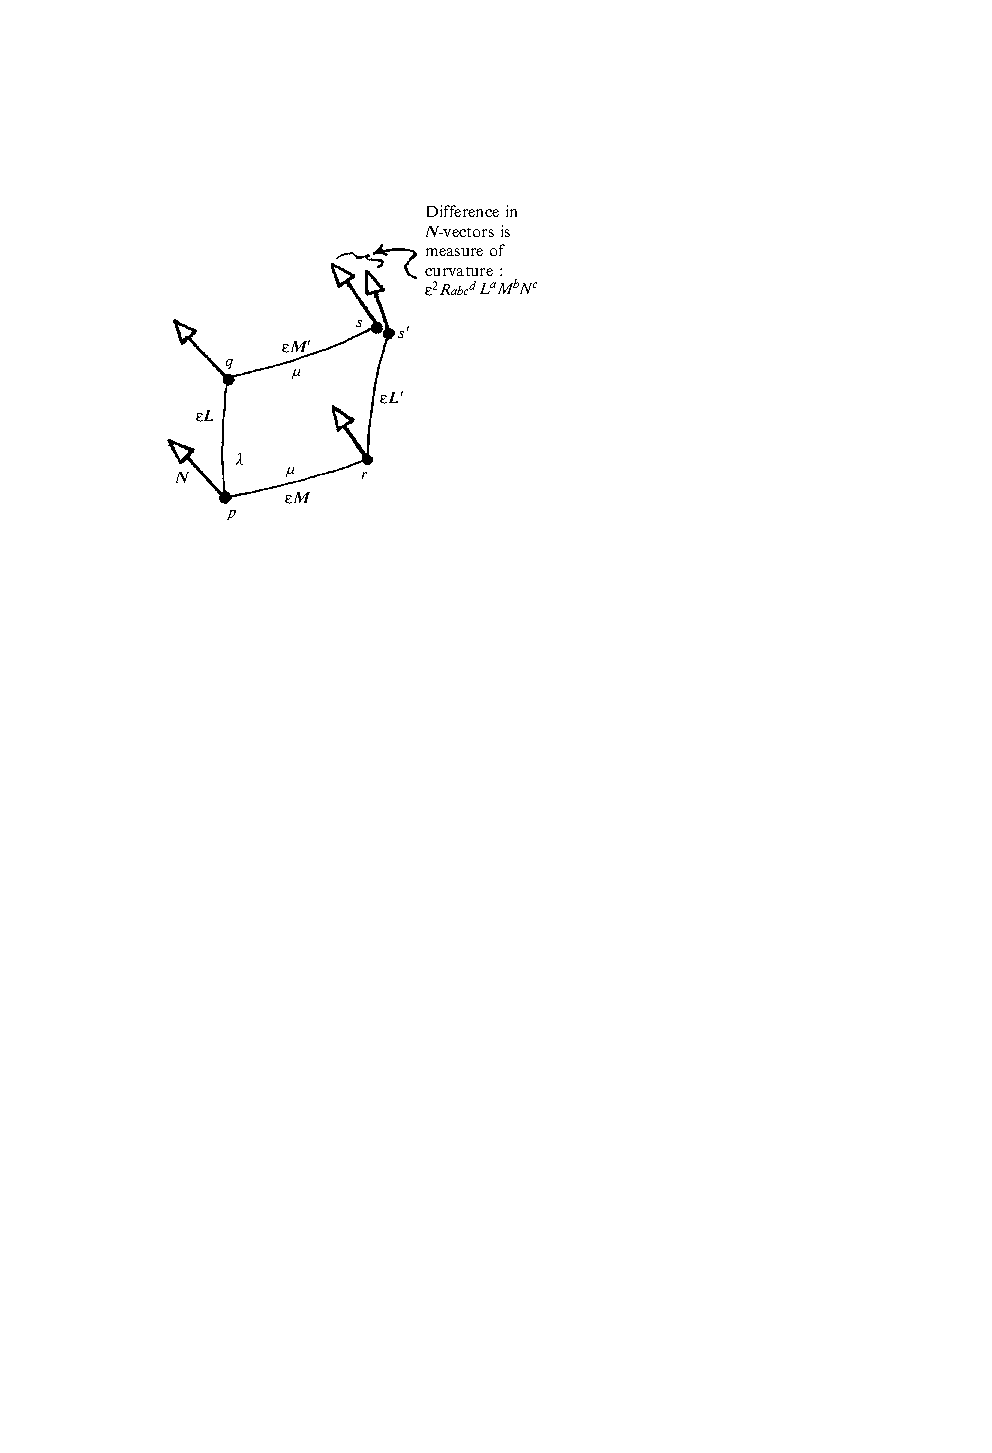
\includegraphics[width=.8\textwidth]{figures/Penrose_Riemann_14_10.pdf}
    \captionsetup{font={scriptsize,sf}}
    \caption{Graphical depiction of what the Riemann tensor from Penrose, \emph{Road to Reality}. Note that Penrose uses a different ordering of indices than we do.}
    \label{fig:Penrose:14:10:Riemann}
\end{marginfigure}
Based on the index structure alone, you can determine that the Riemann tensor can:
\begin{itemize}
    \item Take three vectors and a row vector to return a number, $R^i_{\phantom{i}jk\ell} v^jw^ku^\ell t_i$.
    \item Take two vectors and return a matrix, $R^i_{\phantom{i}jk\ell}v^kw^\ell$. 
    \item Take two vectors and a row vector to return a row vector, $R^i_{\phantom{i}jk\ell}w_iv^ju^k$.
    \item ... and a few more that you can write out. Do not forget contractions of the upper index with one of the lower indices.
\end{itemize}
\begin{newrule}[Tensor contractions]
A $(p,q)$ tensor can contract with $r\leq p$ row vectors and $s \leq q$ column vectors to produce a $(p-r, q-s)$ tensor. By allowing `traces' of the tensor's own upper and lower indices, you can also produce $(p-r-n, q-s-n)$ tensors so long as $p-r-n\geq 0$ and $q-s-n\geq 0$.
\end{newrule}
\begin{exercise}
You can generalize the above rule by allowing a $(p_1,q_1)$ tensor to contract with a $(p_2, q_2)$ tensor. Write out some of the ways in which a $(2,2)$ tensor can contract with a $(1,3)$ tensor. Here is one example: $T^{ij}_{\phantom{ij}k\ell} S^\ell_{\phantom{\ell}ijm}$. 
\end{exercise}
You can see that tensor contraction can get a little dicey. There is a cute graphical notation called birdtracks notation to keep track of this that never became popular.\sidenote{The cover image for these notes is an example of one such contraction. You can learn more about this in Penrose's \emph{Road to Reality}.} In this course we do not worry about very complicated contractions and can stick to index notation.


\subsection{A prelude to symmetry}
\label{sec:isometry:first:pass:indices}
Some ideas are so significant that we introduce them multiple times. Let us preview a key idea: an \textbf{isometry}\index{isometry} is a special symmetry that some vector spaces may have.\sidenote{Specifically, vector spaces equipped with an inner product---called metric spaces---may have isometries.} Let us not concern ourselves for now with the conditions for when such symmetries exist. Instead, for this first pass let us say that isometries are generalizations of rotations.  Take a moment to review the `matrix multiplication' picture of rotations in Section~\ref{sec:Euclidean:three:space:rotations}: rotations $R$ satisfy $R^\trans R = \one$ and, due to this, they preserve the angle and length of vectors. The preservation of angle and length depend on a definition of the dot product---and we are not doing that just yet. However, we can take the lesson that the dot product takes vectors and creates scalars.\sidenote{Scalar is a fancy name for number. More practically, scalars do \emph{not} change under rotations.}

We know that one way to form numbers from objects that have indices is to contract all available indices. Let us examine the simplest such case: a row vector whose indices are contracted with a column vector: $w_iv^i$. Rotations are transformations that act on both row vectors and column vectors. Because row and column vectors are two separate classes of tensorial objects, we allow for the possibility that row vectors and column vectors transform differently:
\begin{align}
    v^i &\to v'^i \defeq R\aij{i}{j}v^j & w_i &= \to w'_j\defeq w_j \tilde{R}\aij{j}{i} \ ,
    \label{eq:components:of:vector:and:row:under:rotatino}
\end{align}
where $R$ and $\tilde{R}$ are the matrices that encode the linear transformation on vectors and row vectors respectively.\sidenote{Neither of these have anything to do with the Riemann curvature tensor, which unfortunately is denoted with an $R$.} We write $v'^i$ and $w'_j$ to be the components of the rotated $v^i$ and $w_j$. Inspired by our earlier intuition that rotations should preserve the value of `fully contracted' objects,\sidenote{All tensor indices are contracted, no free indices.} we can demand that
\begin{align}
    w_i v^i =w'_i v'^i = R\aij{i}{j}v^j \, w_k\tilde{R}\aij{k}{i}
    =\tilde{R}\aij{k}{i}R\aij{i}{j} w_kv^j \ .
    \label{eq:rotations:index:preserve:inner:product:01}
\end{align}
Let us do something silly. We would like to `do algebra' on this equation, which means I would like to cancel out common factors on each side. I would like to cancel the $w_i$ and $v^i$ on the left with the $w_kv^j$ on the right. I can relabel dummy indices,\sidenote{By `dummy index' I mean contracted indices where the choice of variable name does not matter. Though every time I say `dummy index' I think about the `dummy plug' program in \emph{Neon Genesis Evangelion}.} but we need to break apart the fact that $w_i$ and $v^i$ have the same index on the left-hand side. To do this, we multiply by one using the Kronecker-$\delta$: $w_iv^i = w_i \delta^i_j v^j$. Then we may rewrite  \eqref{eq:rotations:index:preserve:inner:product:01} as
\begin{align}
    \cancel{w_i} \cancel{v^j}  \delta^i_j
    =\tilde{R}\aij{i}{\ell}R\aij{\ell}{j} \cancel{w_i} \cancel{v^j} \ ,
\end{align}
from which we have simply:
\begin{align}
    \tilde{R}\aij{i}{\ell}R\aij{\ell}{j} &= \delta^i_j \ .
    \label{eq:R:Rtilde:transformation:from:indices:rotation}
\end{align}
Comparing to \eqref{eq:index:matrix:inverse}, we see that this is the statement that $\tilde R = R\inv$. We have come to a key observation:
\begin{quote}
Under a rotation, an object with an upper index transforms with some matrix $R$ that encodes the rotation. An object with a lower index then transforms with the inverse matrix, $R\inv$. In this way, when a row vector and column vector have their indices contracted, they produce a number that is \emph{invariant} (unchanged) under rotations.
\end{quote}
This observation actually generalizes:
% 
\begin{newrule}[Transformation of upper and lower indices under rotations]
\label{idea:transformation:of:upper:and:lower:indices}
Under an isometry (such as a rotation) $R$, a tensorial object transforms as follows
\begin{align}
    T\aij{i_1\cdots i_N}{j_1\cdots j_M}
    \to 
    R\aij{i_1}{k_1}\cdots R\aij{i_N}{k_N}
    (R\inv)\aij{\ell_1}{j_1}\cdots (R\inv)\aij{\ell_M}{j_M}
    T\aij{k_1\cdots k_N}{\ell_1\cdots \ell_M} \ .
    \label{eq:transformation:of:upper:and:lower:indices}
\end{align}
That is to say: each upper index is contracted with a rotation $R$ and each lower index is contracted with an inverse rotation $R\inv$. 
\end{newrule}

\begin{exercise}
Show that for the case of $2\times 2$ rotations, the inverse is equivalent to the transpose. This turns out to be true for any rotation matrix in Euclidean space.
\end{exercise}

\begin{exercise}
Show that our rule for how row vectors transform can be written in matrix notation as:
\begin{align}
    \row{w} \to \row{w}' \equiv \row{w} R^\trans \ .
\end{align}
To do this, show that the index contracts correspond to the right-hand side. Use the result of the previous exercise that $R\inv = R^\trans$ for rotations.
In this way, it is clear that $\row{w}\vec{v} = \row{w'}\vec{v'}$ is invariant under rotations:
\begin{align}
    \row{w'}\vec{v'} = \row{w}R^\trans R\vec{v} = \row{w} \one \vec{v} \ ,
\end{align}
where we use the definition \eqref{eq:RTR:one}.
\end{exercise}





\section{Vector Space}

If you have some vectors, the combined set of all possible linear combinations of those vectors is called a \textbf{vector space}. This is the idea introduced in Section~\ref{sec:linear:combination:and:span}. Suppose you have some vectors\sidenote{Note that the lower index here is \emph{not} a component index! The vector $\vec{v_2}$ has components $(v_2)^1, (v_2)^2, \cdots$.},  $\vec{v}_1, \cdots, \vec{v}_N$. From these vectors, you can form an infinite number of other vectors by choosing numbers $\alpha^i$ and forming the linear combination
\begin{align}
    \alpha^1 \vec{v}_1 + \alpha^2\vec{v}_2 + \cdots + \alpha^N \vec{v}_N \ .
    \label{eq:linear:combination:looks:like:basis}
\end{align}
The set of all possible vectors that can be formed this way is called the \textbf{vector space} \emph{spanned by}  $\vec{v}_1, \cdots, \vec{v}_N$. The word \textbf{span}\index{span} means the vector space of all linear combinations of a set of vectors. When we say that \emph{linear combinations of vectors are also vectors}, what we mean is that they are \emph{also vectors in the vector space}. We write vector spaces with a capital letter, say $V$, and write that a vector $\vec{v}$ is part of the vector space by writing
\begin{align}
    \vec{v} \in V \ .
\end{align}

\begin{example}
If you have two vectors,
\begin{align}
    \vec{v} &= 
    \begin{pmatrix}
        3 \\ 1 \\ 0
    \end{pmatrix}
    &
    \vec{w} &= 
    \begin{pmatrix}
        2 \\ 1 \\ 3
    \end{pmatrix}
    \label{eq:eg:of:vector:space:1}
\end{align}
then you could form another vector that is a linear combination of the two:
\begin{align}
    2\vec{v} - 1 \vec{w}
    =
    \begin{pmatrix}
        4 \\ 1 \\ -3
    \end{pmatrix} \ .
\end{align}
We say that this vector is part of the vector space $V$ spanned by $\vec{v}$ and $\vec{w}$. 
\end{example}

\begin{example}
If $V$ is the vector space spanned by by $\vec{v}$ and $\vec{w}$ in \eqref{eq:eg:of:vector:space:1}, then the vector
\begin{align}
    \vec{u}
    =
    \begin{pmatrix}
        3 \\ 1 \\ 2
    \end{pmatrix} \ .
\end{align}
is \emph{not} part of the vector space $V$ because there are no coefficients $\alpha^1$ and $\alpha^2$ that can satisfy
\begin{align}
    \alpha^1\vec{v} + \alpha^2 \vec{w} = \vec{u} \ .
\end{align}
If you are not convinced, please try it. In the above condition, how many unknowns are there? How many component-level constraint equations are there?
\end{example}

\begin{example}
Consider the vectors
\begin{align}
    \vec{a}
    &=
    \begin{pmatrix}
        1\\0
    \end{pmatrix}
    &
    \vec{b}
    &=
    \begin{pmatrix}
        0\\1
    \end{pmatrix}
    &
    \vec{c}
    &=
    \begin{pmatrix}
        1\\1
    \end{pmatrix}\ .
\end{align}
The vector space spanned by these three vectors is \emph{all} of the two-component vectors. In fact, the vector space spanned by any \emph{two} of these vectors is all of the two-component vectors. 
\end{example}


By this notion of duality, you should expect that row vectors also form a vector space. If the space of column vectors is called $V$, then the space of row vectors is called $V^*$. Evidently there is some relation between the two, even though they appear be totally different vector space.\sidenote{That is: we could have just said that row vectors live in a vector space $W$ and $W$ has nothing to do with $V$.} Indeed, the relation is that that row vectors can contract with column vectors. The star evidently means the space of \emph{vectors that can contract with this other set of vectors}. In this way, column vectors are the dual space of row vectors: $(V^*)^* = V^{**} = V$. This is simply saying that in the contraction $w_i v^i$, we can think of $w_i$ acting on $v^i$ or we can equivalently think of $v^i$ acting on $w_i$. 


\section{Basis of a Vector Space}\label{sec:basis}

Let us return to \eqref{eq:linear:combination:looks:like:basis}. Take a moment to take a good look at that equation. In fact, this equation is so important that we write it out again:
\begin{align}
    \alpha^1 \vec{v}_1 + \alpha^2\vec{v}_2 + \cdots + \alpha^N \vec{v}_N \ .
    \tag{\ref{eq:linear:combination:looks:like:basis}}
\end{align}
Here are a few thoughts that may come to your mind while looking at this linear combination of vectors.
\begin{enumerate}
    \item Hmm. We have $N$ vectors and took a linear combination of them. This means that we needed $N$ coefficients. Rather than writing $\alpha$, $\beta$, $\gamma$, and so forth, we chose to jsut label them all $\alpha$ but with an upper index. 
    \item Oh... the upper index is convenient because it means we can write the linear combination as $\alpha^i \vec{v}_i$. But this isn't a ``real'' contraction, right? Well... it follows the summation convention so I suppose that's legitimate. It is just weird that $\vec{v}_i$ is an entire vector with and additional lower index.
    \item In fact, these $\alpha^i$ coefficient look suspiciously like the components of a vector.
    \item Wait a second, $\alpha^i\vec{v}_i$ \emph{is} a vector.
    \item Can I think about $\alpha^i$ as being the components of the vector $\alpha^i\vec{v}_i$?
\end{enumerate}


\subsection{An understanding between friends}
This brings us to the critical idea of a basis. Now is a good time to go over the examples in the previous section. Go ahead and do that. \emph{Right now.} Okay, welcome back. Suppose that you and I agreed on a set of vectors. Let's say that we both agreed on the $N$ vectors in \eqref{eq:linear:combination:looks:like:basis}; we even agree on the numbering. Let us call this special set of vectors a \textbf{basis}\index{basis}. That means that if I want to communicate to you some linear combination of those vectors, all I have to do is give you a list of their coefficients. I would write this as a column,
\begin{align}
    \vec{a} = 
    \begin{pmatrix}
        \alpha^1\\
        \vdots \\
        \alpha ^N
    \end{pmatrix} \ .
\end{align}
You may say: oh, that's an odd way to write a linear combination---just stacking the coefficients in a column like that. But sure, we both understand that what this \emph{really} means is
\begin{align}
    \vec{a} = 
    \alpha^i \vec{v}_i \ ,
\end{align}
we can just leave the $\vec{v}_i$ implicit because we both already agree on what those vectors are. 

Maybe you see what is going on here. We previously introduced vectors as columns of numbers. Now we are saying that columns of numbers represent a particular linear combinations of basis vectors. It seems that all this time, the `column of numbers' that we started actually mean a linear combination of a specific choice of basis vectors. In fact, the standard or canonical basis vectors can be thought of as columns:
\begin{align}
    \bas{e}_1 &= 
    \begin{pmatrix}
        1\\ 0 \\  0 \\\vdots
    \end{pmatrix}
    &
    \bas{e}_2 &= 
    \begin{pmatrix}
        0 \\ 1 \\  0 \\\vdots
    \end{pmatrix}
    &
    \bas{e}_3 &= 
    \begin{pmatrix}
        0 \\ 0 \\  1 \\\vdots
    \end{pmatrix}
    &
    \cdots
    \label{eq:canonical:basis}
\end{align}
We have moved to a notation where we write the basis vectors as $\bas{e}_i$. A basis does not \emph{need} to be nice. 


In terms of the canonical basis \eqref{eq:canonical:basis}, we now understand that the components of a vector mean
\begin{align}
    \vec{v} = v^1 \bas{e}_1 + v^2 \bas{e}_2 + \cdots = v^1 \bas{e}_1 \ .
\end{align}

\begin{bigidea}[The big deal about bases]\label{idea:reasons:to:like:bases}
This whole hubbub about bases is useful for at least two reasons:
\begin{enumerate}
    \item This notion completely abstracts away the \emph{meaning} of a vector. The basis vectors carry all the `vector-ness'\sidenotemark of the vector. 
    \item If you and I are \emph{not} using the same basis, then all I have to do is convert your basis into my basis to be able to convert your components into my components.
\end{enumerate}
\end{bigidea}\sidenotetext{Or more generally, tensor-ness.}

We briefly introduce these two ideas in turn. But first, let us address the index structure of the basis.

\paragraph{Why do basis vectors have lower indices?} Previously we said objects with a single lowered index are row vectors. Are basis vectors row vectors? Not quite. In fact, when we talked about tensors, we said that the specific component $T^{i_1\cdots i_N}_{\phantom{{i_1\cdots i_N}}j_1\cdots j_M}$ is just some number. For basis vectors, once we specify $i$, $\bas{e}_i$ is \emph{not} a number: it carries all of the \emph{meaning} of what a vector \emph{is} in whatever context the vector is being used. The basis vector has a lower index because it means we can contract it with the upper index of $v^i$. The resulting object is the vector itself, $\vec{v}$ which carries no indices. If this sounds like philosophical navel gazing, please jump ahead and do Exercise~\ref{ex:fibonacci:space}---it is a rather different example of `vector-ness' than `columns of numbers.'





\subsection{Abstraction}
\label{sec:sub:abstraction:basis}

% In Section~\ref{sec:sub:basis:changing} we saw how making the basis vectors explicit helps us understand how to relate tensors in one reference frame (basis) to another. Recall that there is a second reason in \bigidearef~\ref{idea:reasons:to:like:bases} why basis vectors are helpful: they
Basis vectors help us further let vectors become more abstract.\sidenote{There is an analogy here to the \LaTeX typesetting system. The goal of \LaTeX is to separate content from the under-the-hood work to present that content. For practical purposes, we want to separate components---which are just numbers that we can work with---from underlying mathematical machinery that gives those components meaning.}
%
Another way of saying this is as follows:
\begin{quote}
Vectors are \emph{not} columns of numbers.
\end{quote}
Those numbers are the \emph{components} of a vector. But the \emph{meaning} of a vector depends on the context. In some contexts the vector might be a velocity or a momentum. It may be a unit excitation in the electric field. It may be the spin state of an electron. It may be a solution to the spherical Laplace equation. The magic is that all sorts of \emph{physical} quantities are described by vectors. The basis vectors carry these identities so that we can just work with numerical coefficients that we happen to denote with upper indices and that we sometimes arrange in columns.


\paragraph{Arrow space}
Our goal is to abstract away any notion of column vectors. A useful way to think about this is an idea that is perhaps familiar: imagine vectors are arrows with a magnitude and a direction. The rule for adding vectors is that you stack them together, tail-to-head.\sidenote{It should be clear that this definition is commutative, $\vec{v}+\vec{w} = \vec{w}+\vec{v}$.} For example, consider the following basis:
\begin{align}
    \bas{e}_1 &= \eqfig{
\includegraphics[width=2em]{figures/basis_e1.pdf}}
    &
    \bas{e}_2 &= \eqfig{
\includegraphics[width=2em]{figures/basis_e2.pdf}} \ .
\end{align}
Then a vector $\vec{v}$ may be written as a linear combination of those vectors. Figure~\ref{fig:eg:basis:arrows:canonical:eg} demonstrates this.
\begin{marginfigure}%[th]
    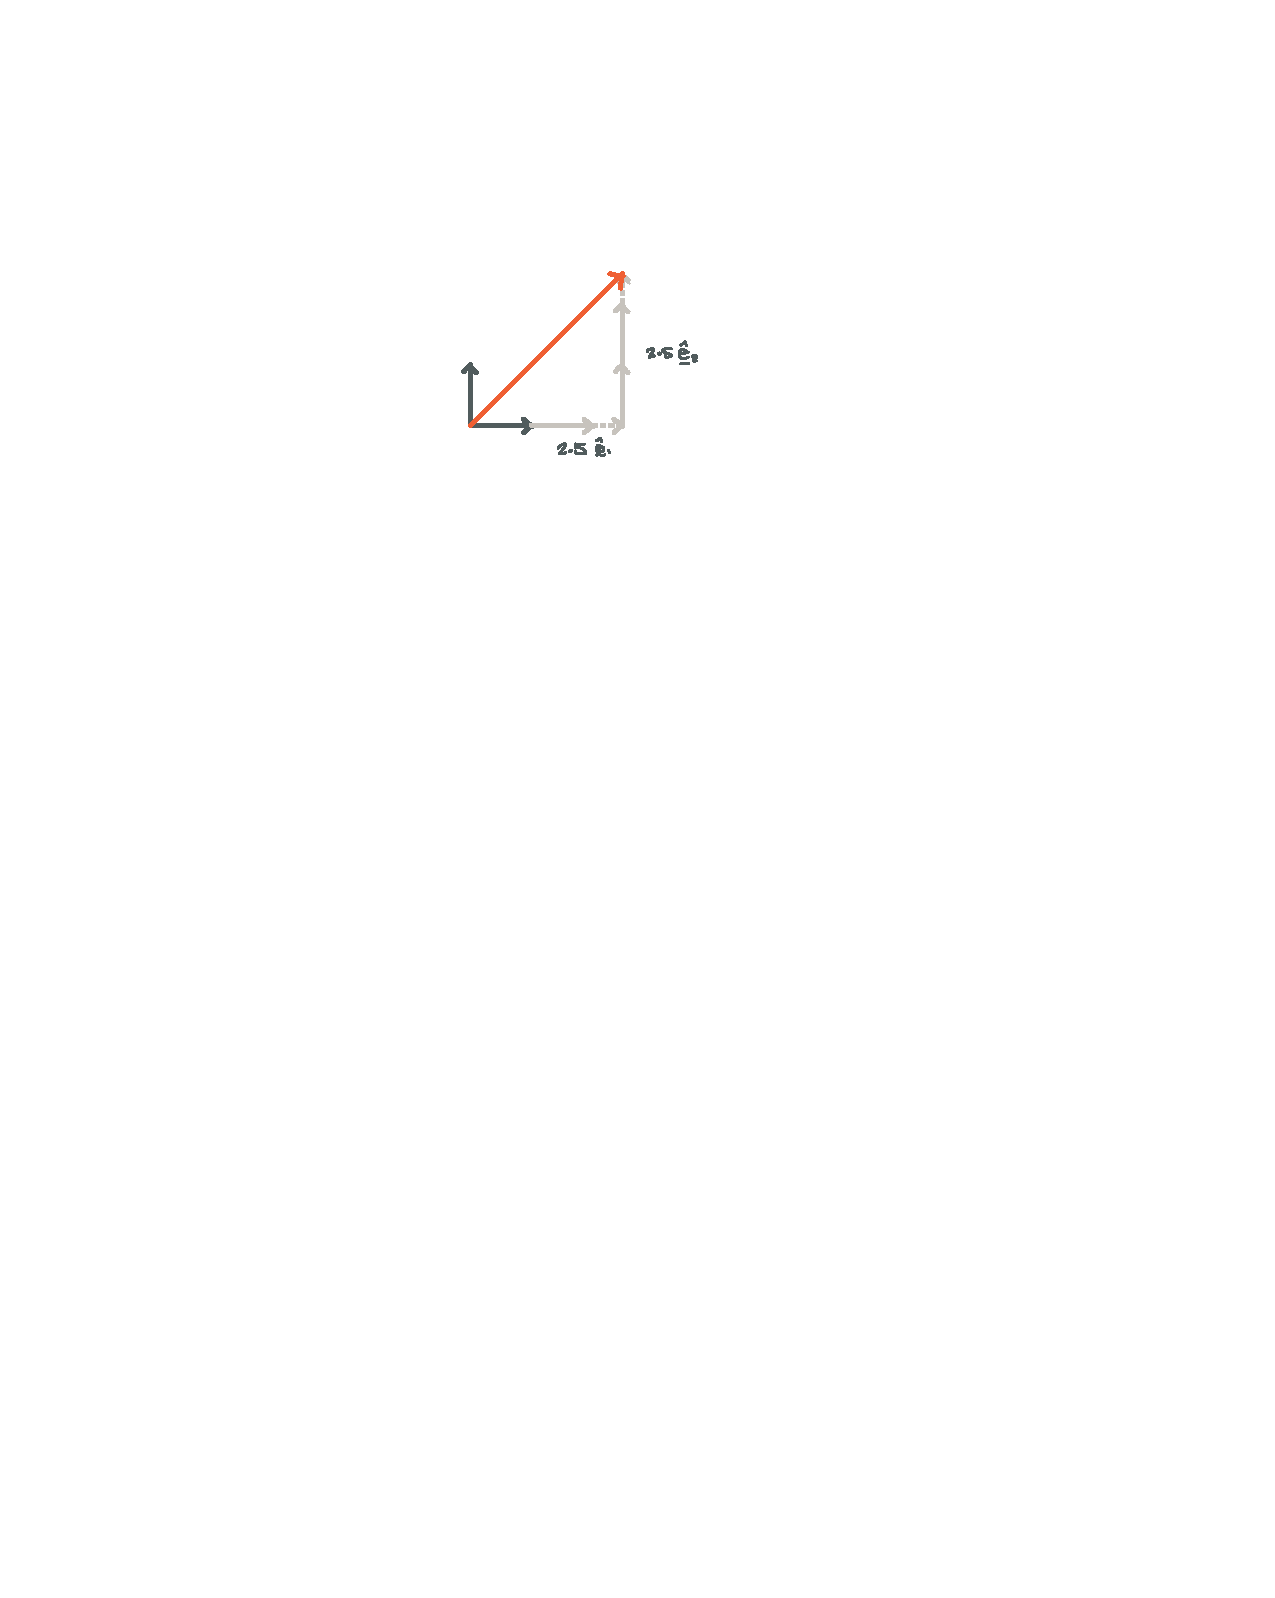
\includegraphics[width=.6\textwidth]{figures/basis_red_e.pdf}
    \captionsetup{font={scriptsize,sf}}
    \caption{The vector $\vec{v}$ (in red) is $2.5\bas{e}_1 + 2.5\bas{e}_2$.}
    \label{fig:eg:basis:arrows:canonical:eg}
\end{marginfigure}
In that example, the components of the vector $\vec{v}$ are
\begin{align}
    \vec{v} &= v^i\bas{e}_i = 2.5 \bas{e}_1 + 2.5 \bas{e}_2  \ .
\end{align}
We could have used a different basis of the same space. This basis is
\begin{align}
    \bas{f}_1 &= \eqfig{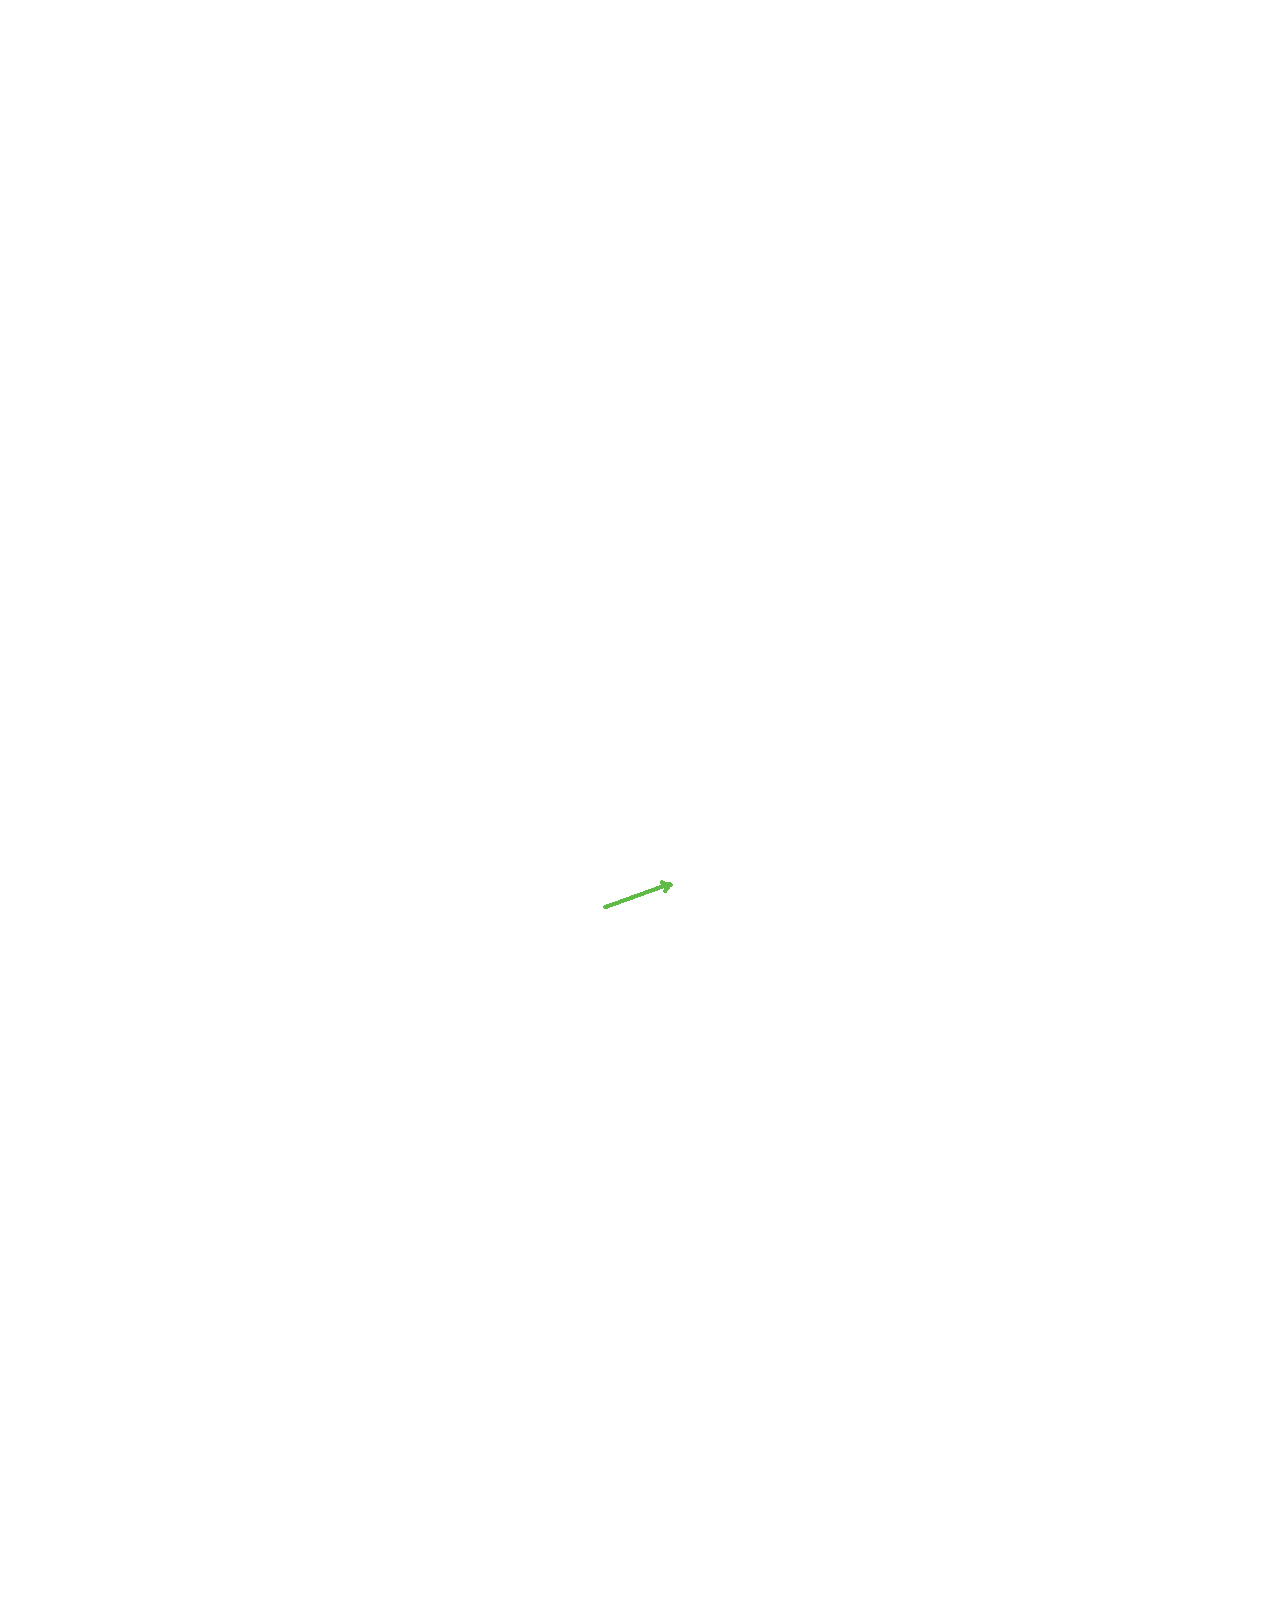
\includegraphics[width=2em]{figures/basisf1.pdf}}
    &
    \bas{f}_2 &= \eqfig{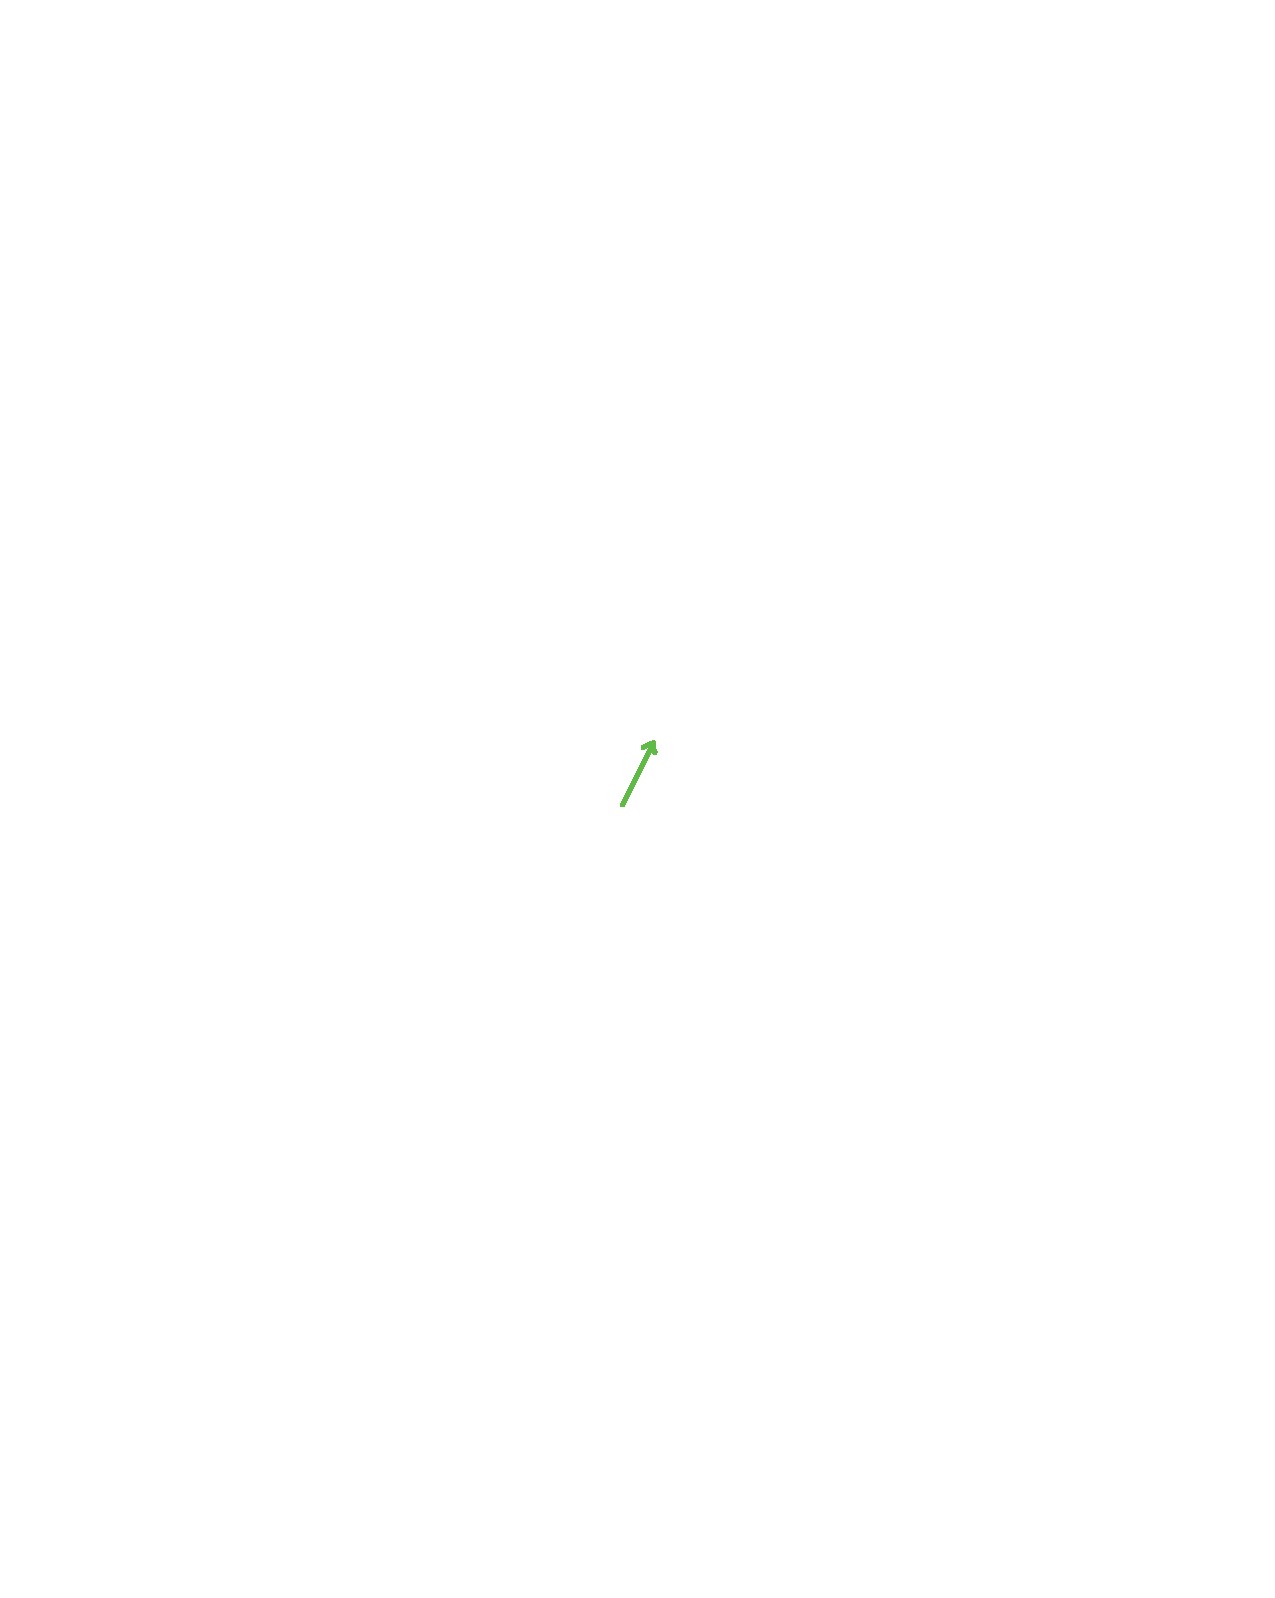
\includegraphics[width=2em]{figures/basisf2.pdf}} \ .
\end{align}
Figure~\ref{fig:eg:basis:arrows:canonical:eg:odd:basis} shows the same vector $\vec{v}$ written as a linear combination of the $\bas{f}_{1,2}$ basis.
\begin{marginfigure}%[th]
    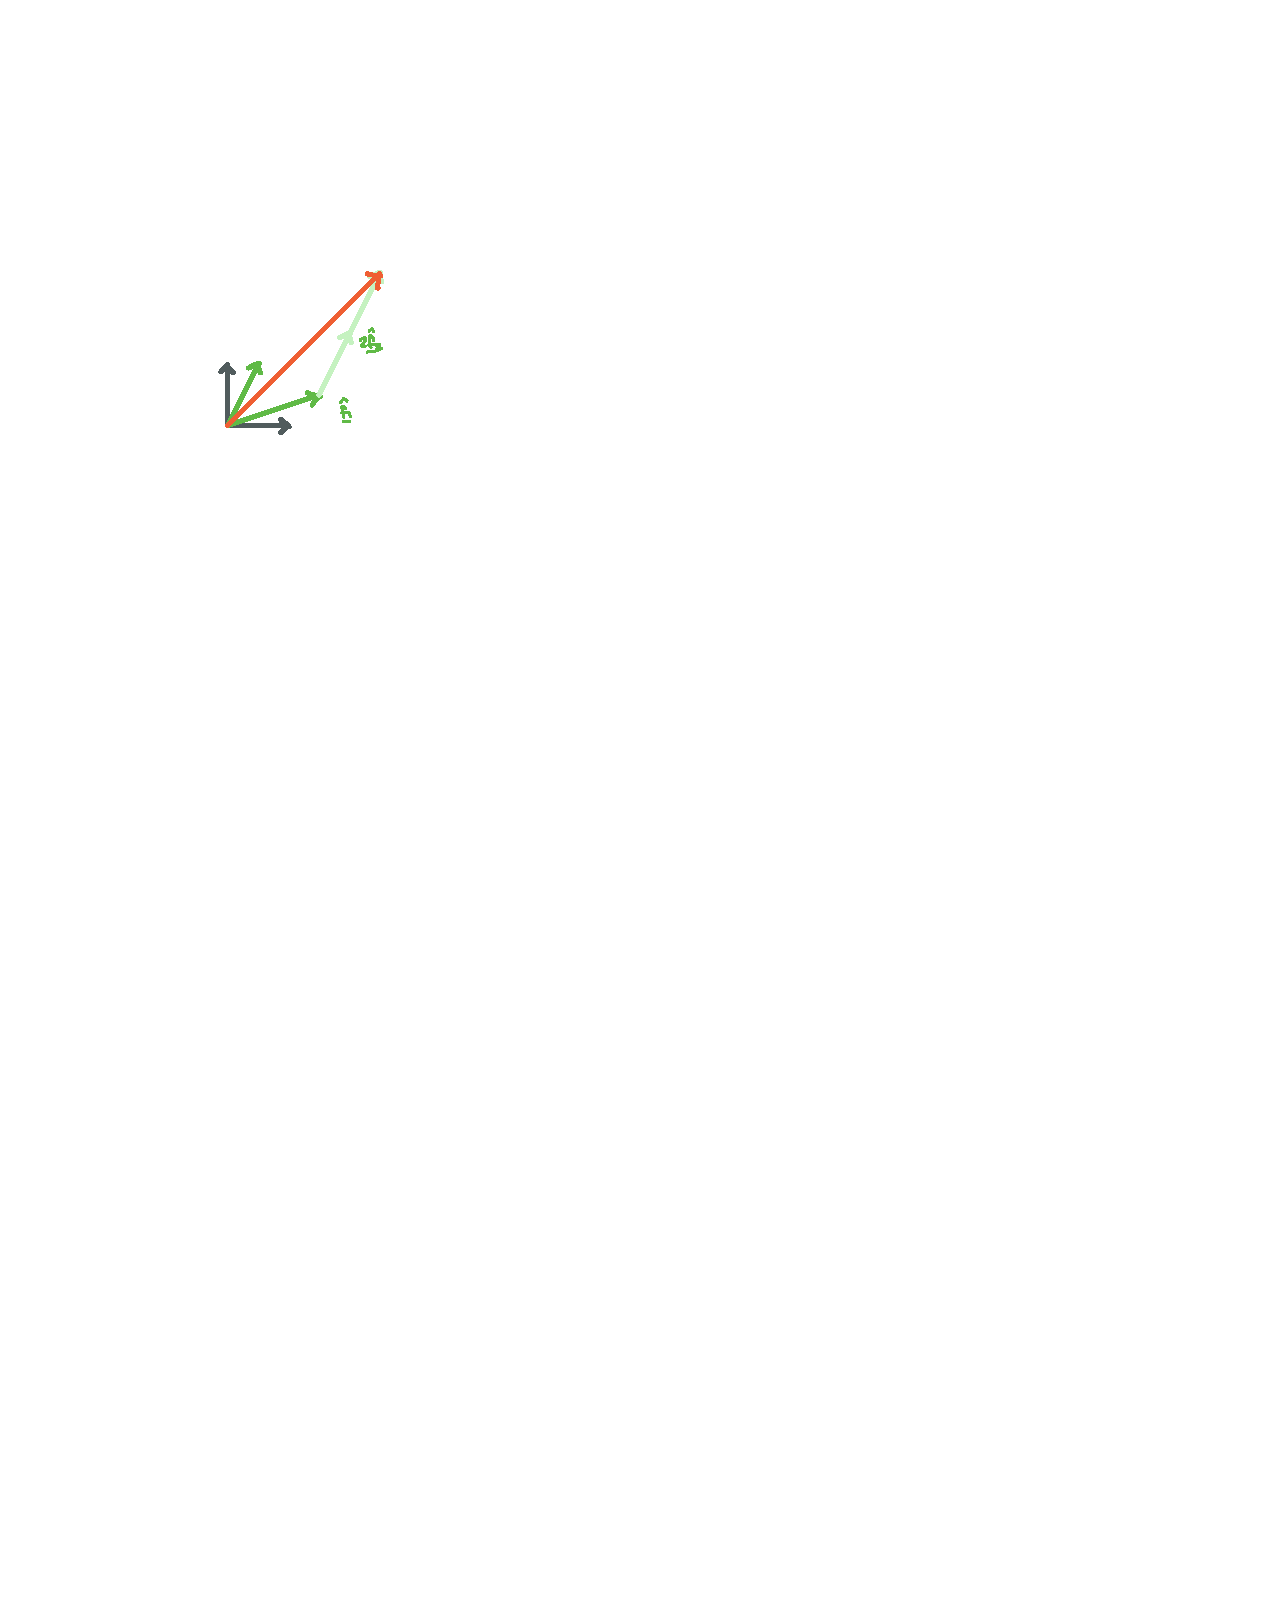
\includegraphics[width=.6\textwidth]{figures/basis_red_f.pdf}
    \captionsetup{font={scriptsize,sf}}
    \caption{The vector $\vec{v}$ (in red) is $\bas{f}_1 + 2\bas{f}_2$.}
    \label{fig:eg:basis:arrows:canonical:eg:odd:basis}
\end{marginfigure}
\begin{align}
    \vec{v} &= v'^i\bas{f}_i =  \bas{f}_1 + 2\bas{f}_2  \ .
\end{align}

As a final demonstration, we illustrate that coefficients of basis vectors may also be negative. In Figure~\ref{fig:eg:basis:arrows:neg} we have a vector in blue that is a positive sum of the $\bas{e}_{1,2}$ basis vectors, but is the linear combination $3\bas{f}_1 - \bas{f}_2$ in the $\bas{f}_{1,2}$ basis.
\begin{marginfigure}%[th]
    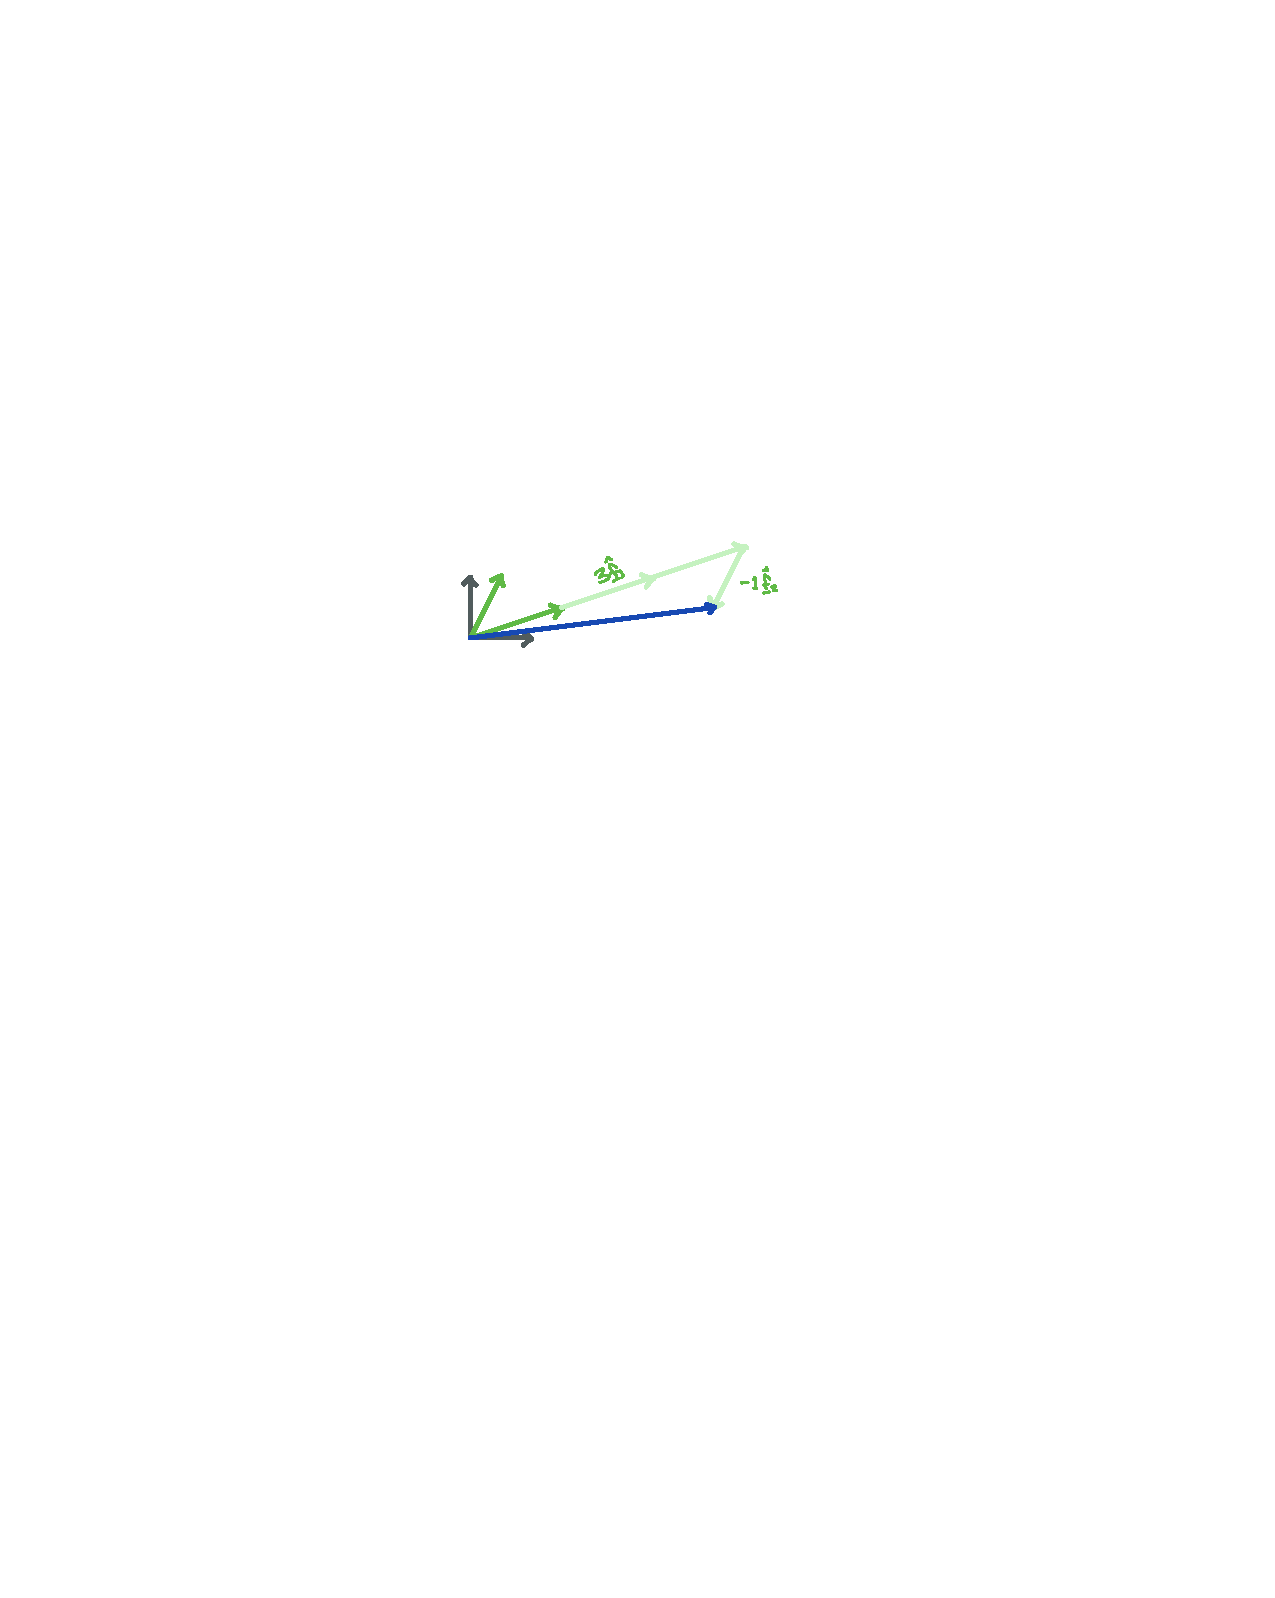
\includegraphics[width=\textwidth]{figures/basis_neg.pdf}
    \captionsetup{font={scriptsize,sf}}
    \caption{Example of a vector (blue) that has a negative coefficient of $\bas{f}_2$ in the $\bas{f}_{1,2}$ basis.}
    \label{fig:eg:basis:arrows:neg}
\end{marginfigure}

\begin{example}\label{ex:cheeseburger:space}
A silly vector space the space spanned by cheeseburgers ($\bas{e}_1$) and fries ($\bas{e}_2$) are your favorite local burger joint:
\begin{align}
\bas{e}_1 &=
    \eqfig{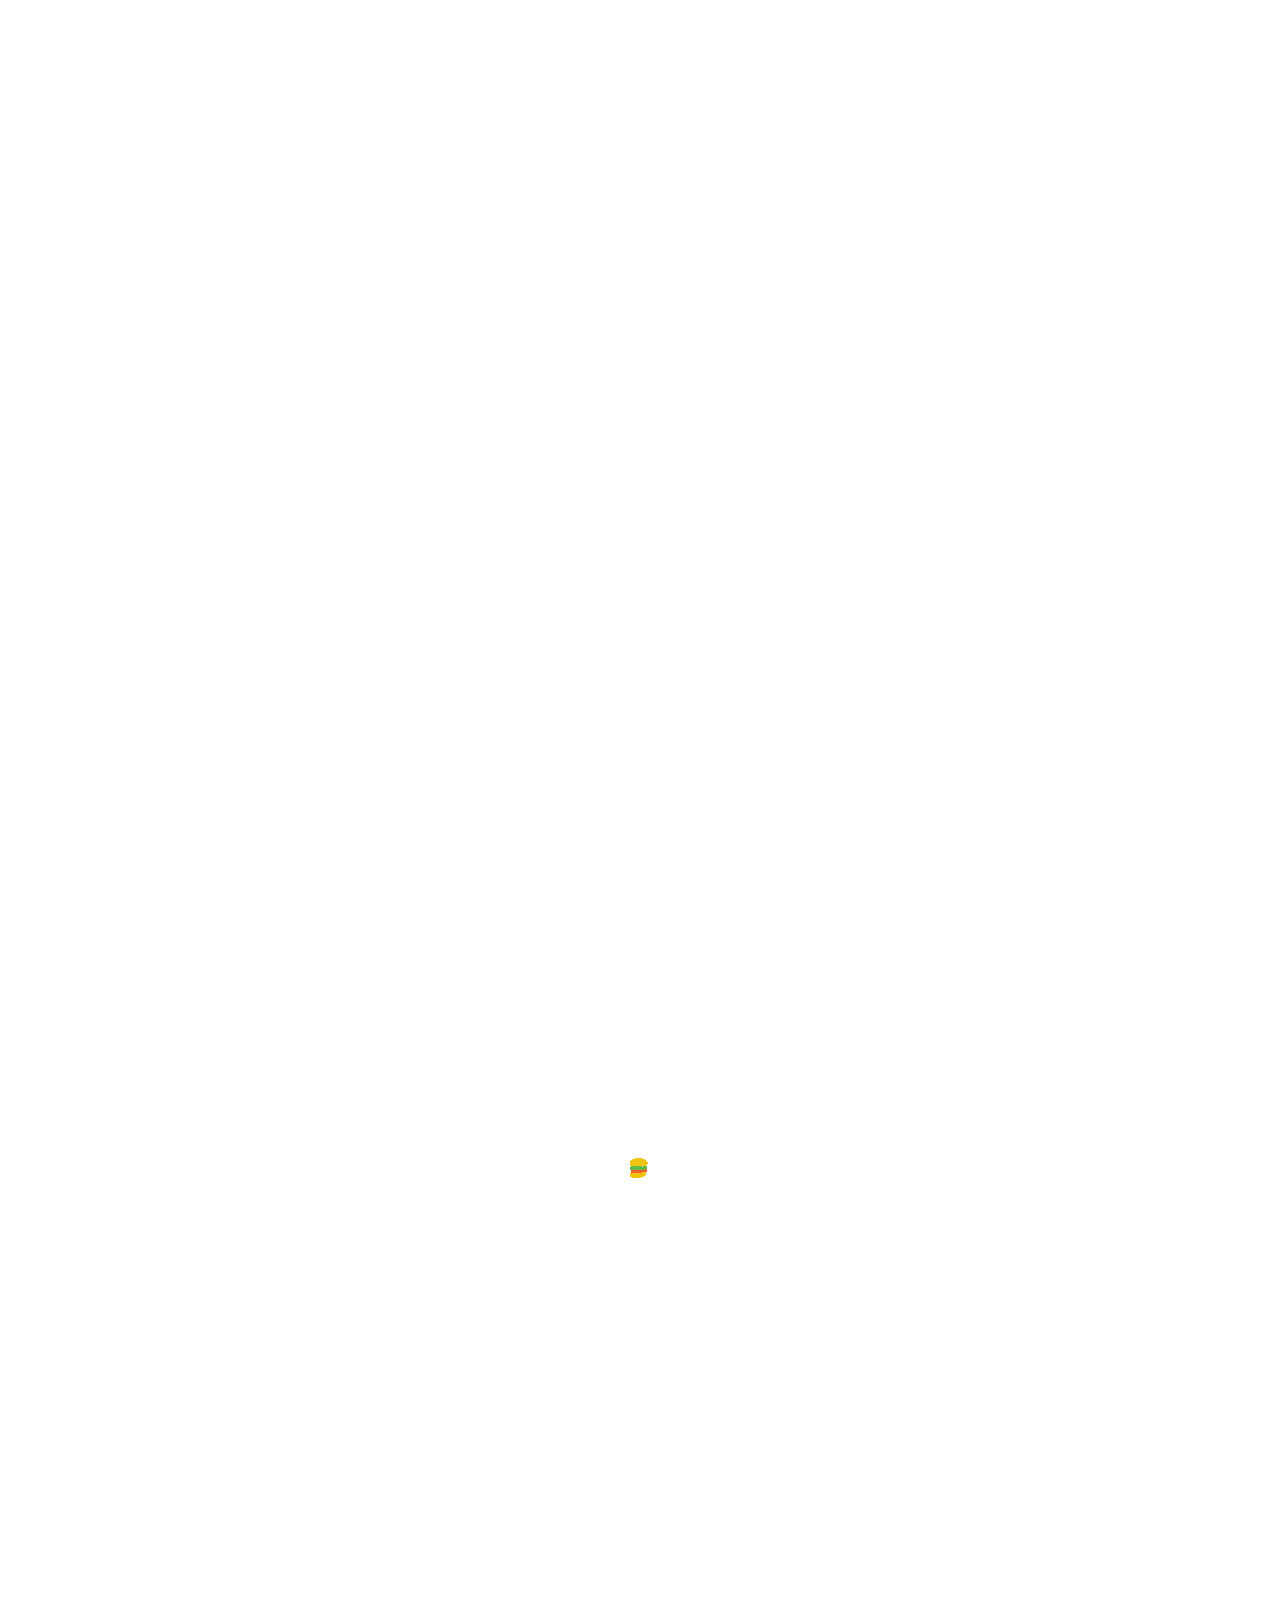
\includegraphics[width=1.5em]{figures/basis_food_icon_burger.pdf}}
    &
    \bas{e}_2 &=
    \eqfig{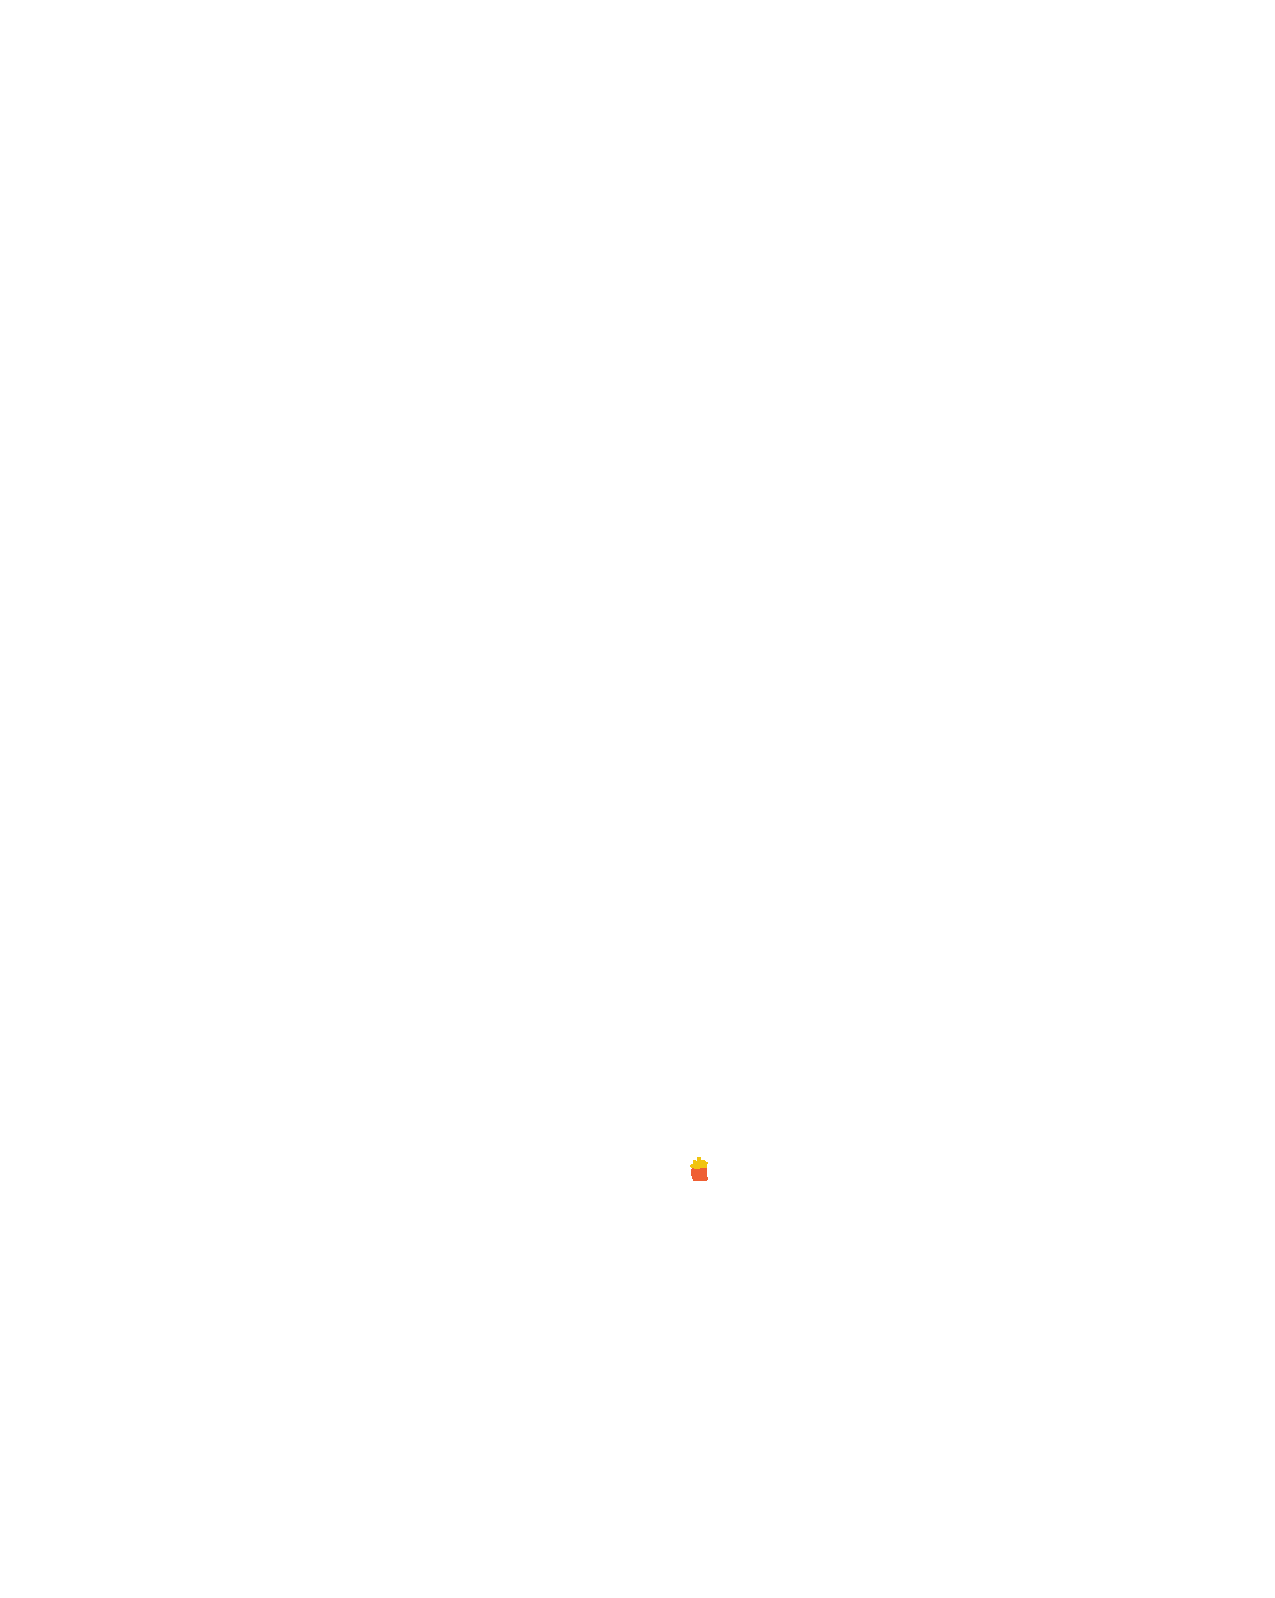
\includegraphics[width=1.5em]{figures/basis_food_icon_fries.pdf}} 
    &
    \eqfig{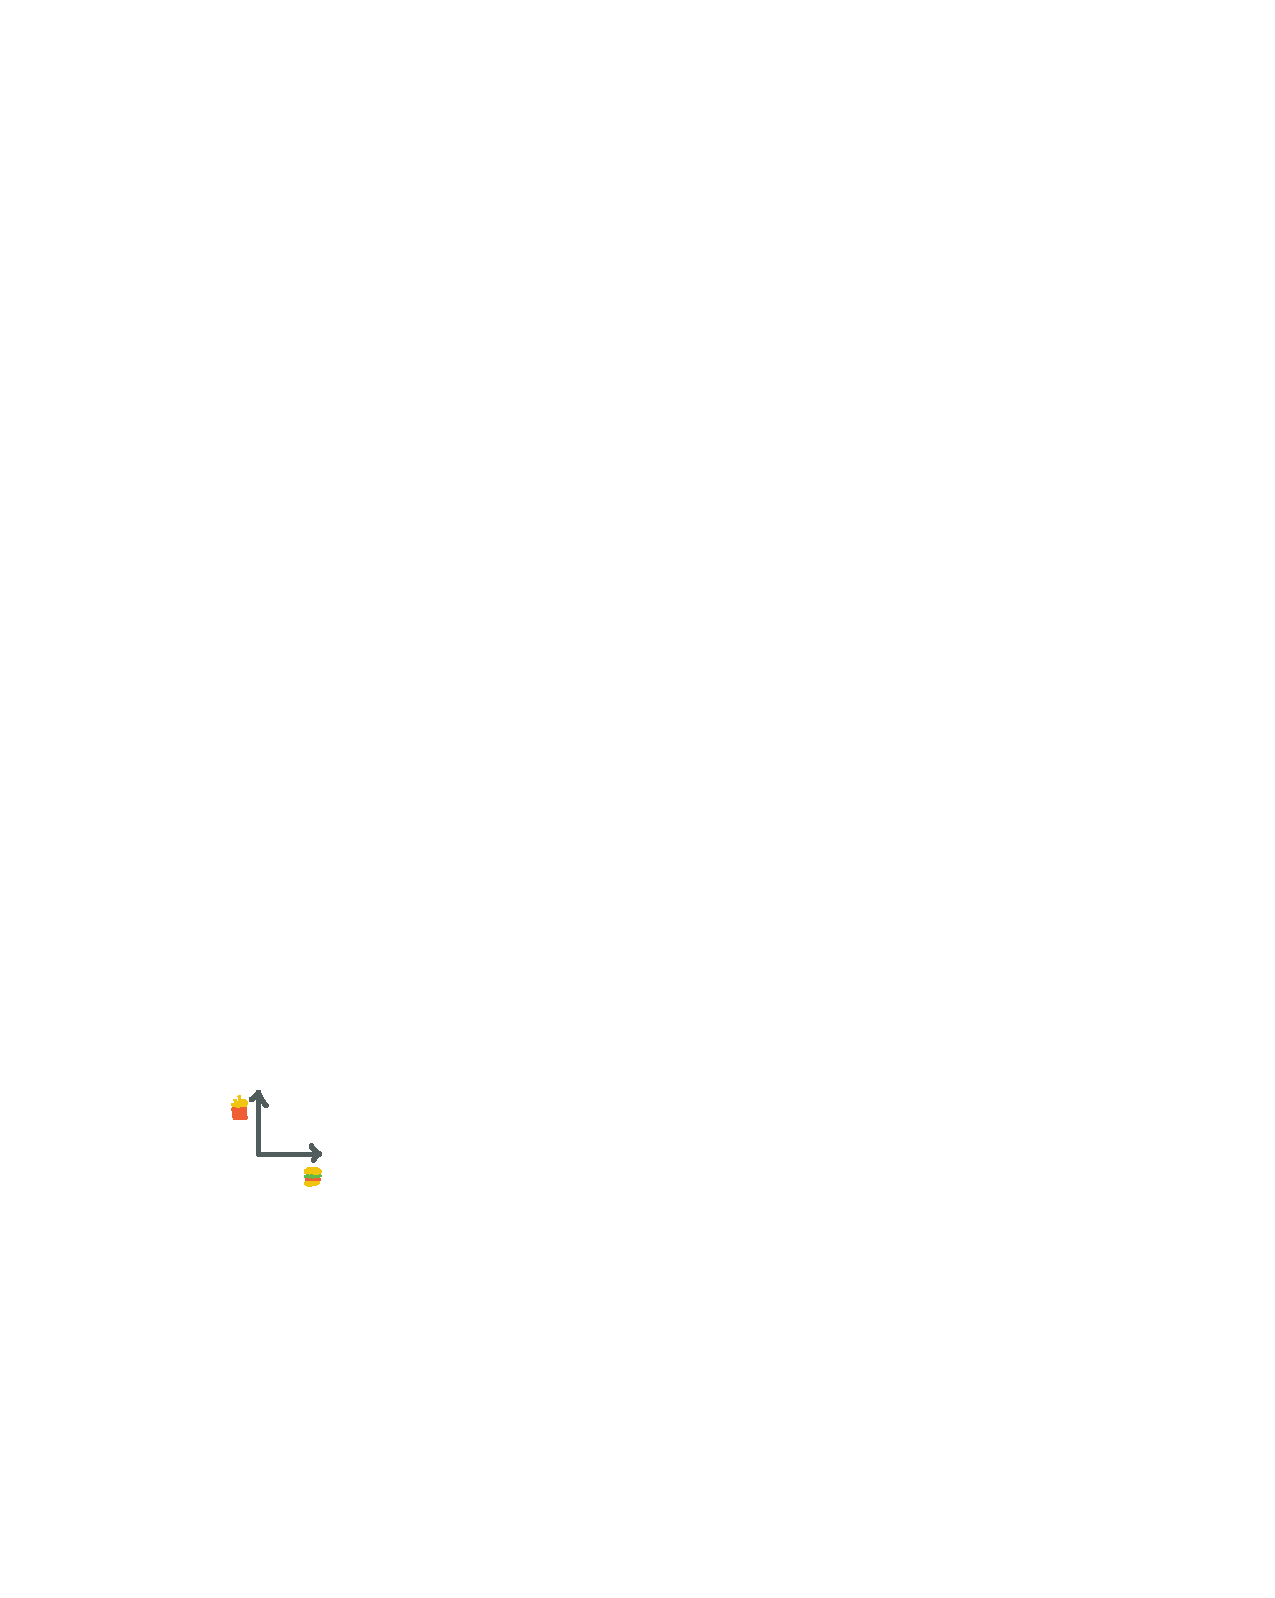
\includegraphics[width=4em]{figures/basis_food_canonical.pdf}} 
    \ .
\end{align}
Then an order $\vec{v}$ of 2 burgers and 1 fries is
\begin{align}
    \vec{v} =
    2\bas{e}_1 + \bas{e}_2 = 
    2\eqfig{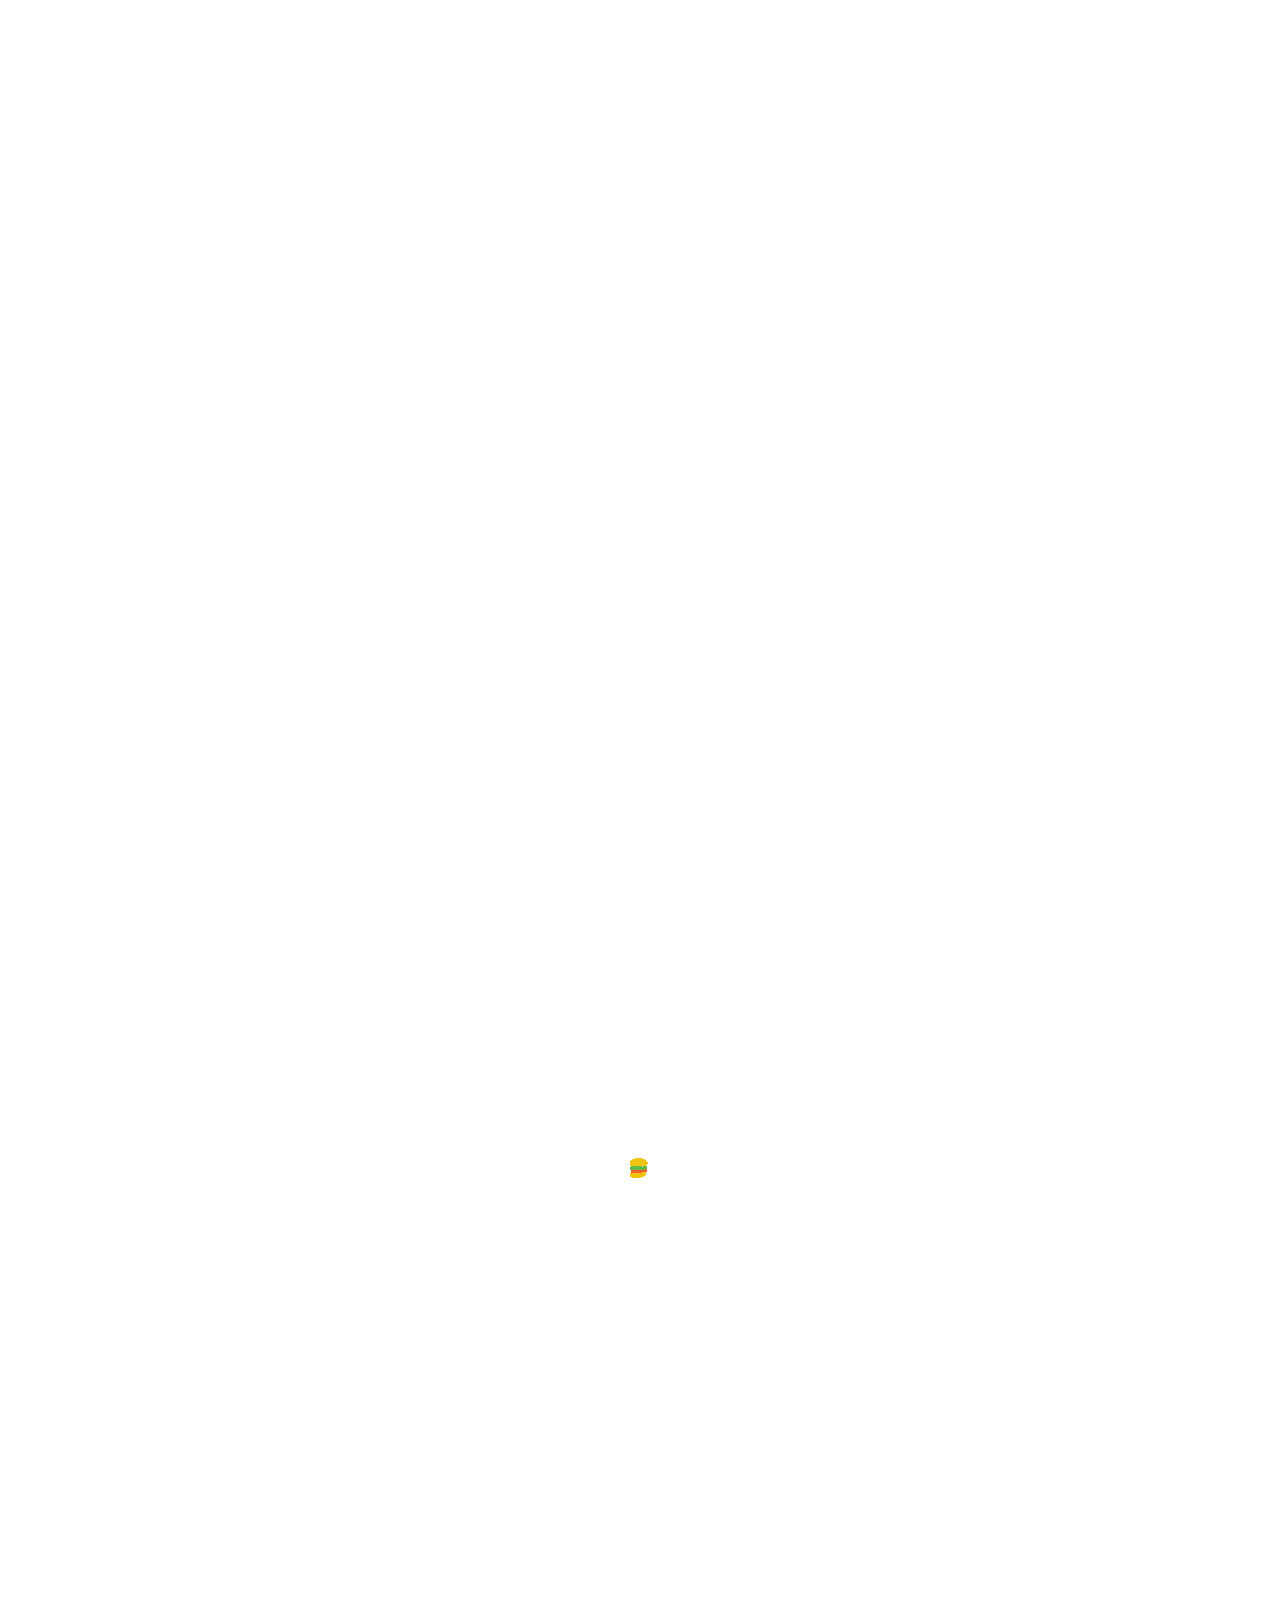
\includegraphics[width=1.5em]{figures/basis_food_icon_burger.pdf}} 
    +
    \eqfig{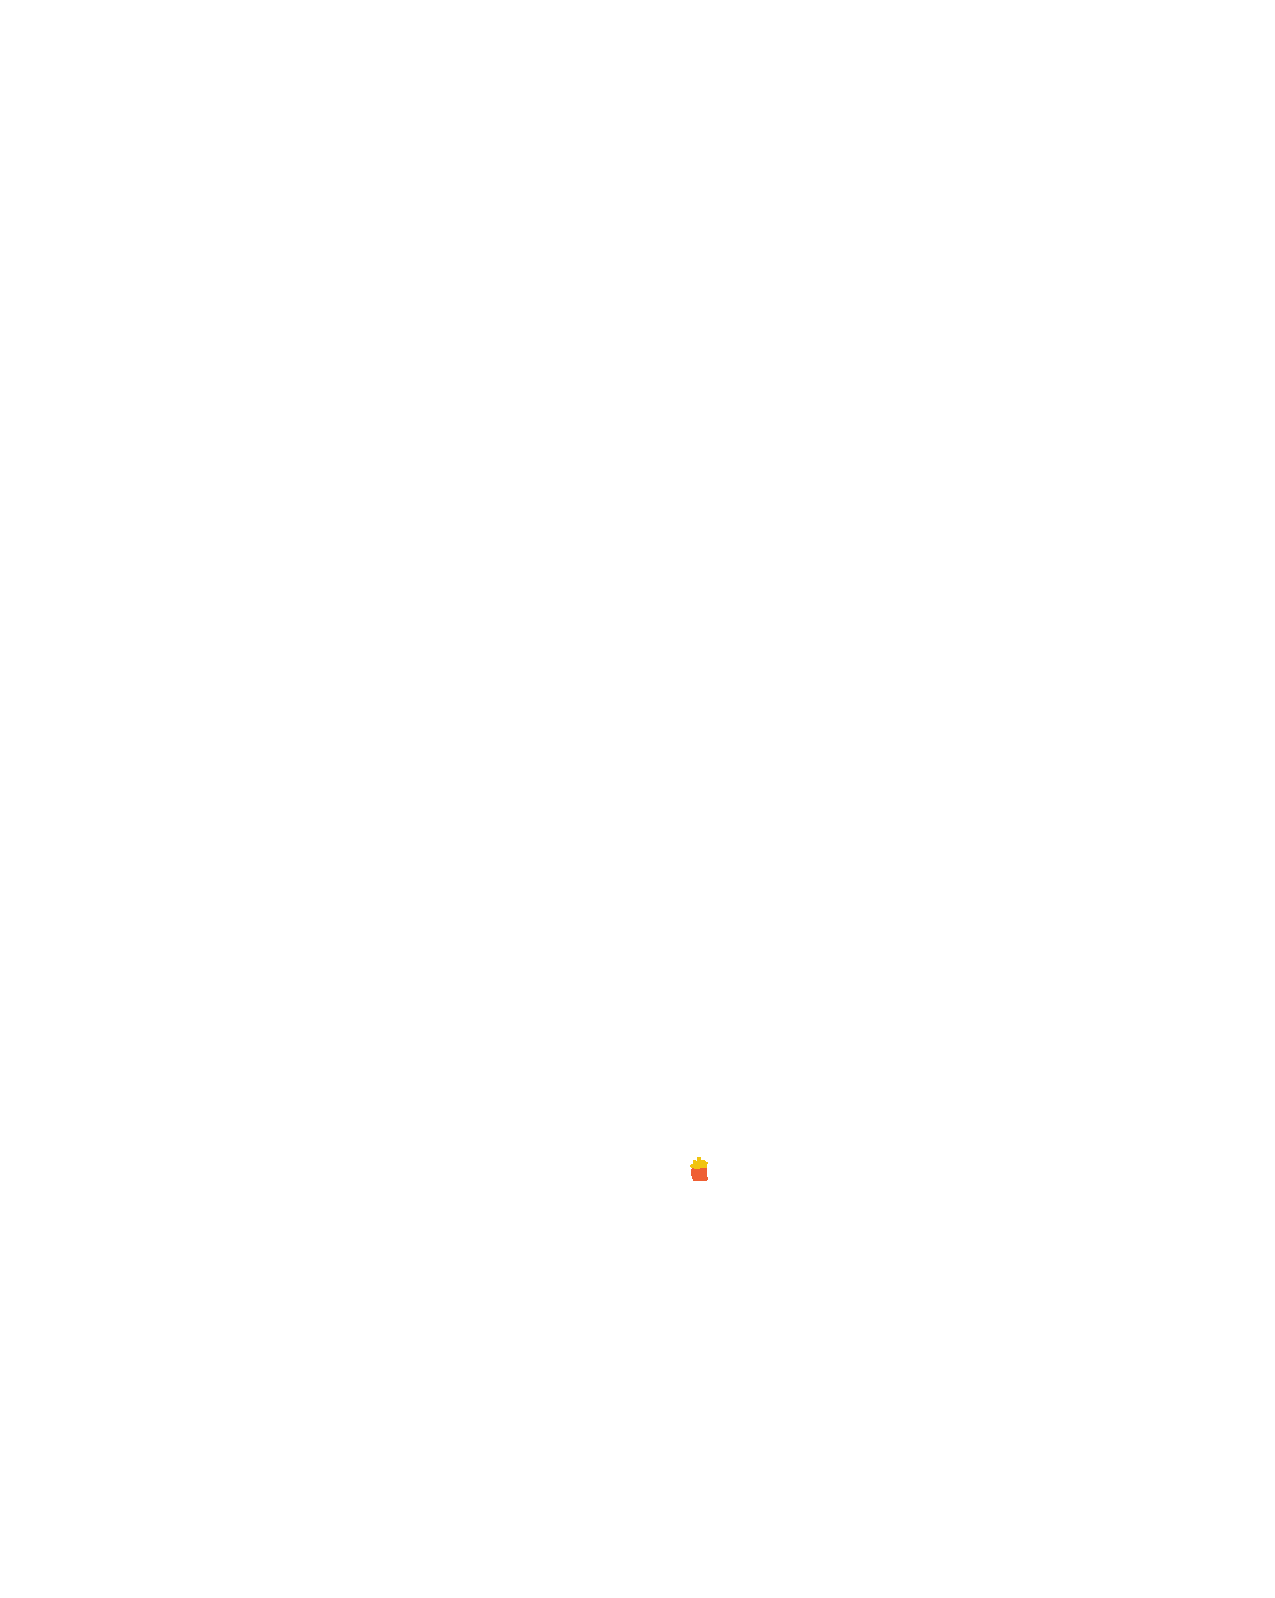
\includegraphics[width=1.5em]{figures/basis_food_icon_fries.pdf}} \ .
    \label{eq:basis:eg:meal:1}
\end{align}
Suppose the burger joint also offers a combo meal that includes one burger and one fries. Then we can choose another basis of combo meals ($\bas{f}_1$) and fries ($\bas{f}_2 = \bas{e}_2$); on the right we show it relative to the other basis:
\begin{align}
\bas{f}_1 &=
    \eqfig{
\includegraphics[width=1.5em]{figures/basis_food_icon_meal.pdf}}
    &
    \bas{f}_2 &=
    \eqfig{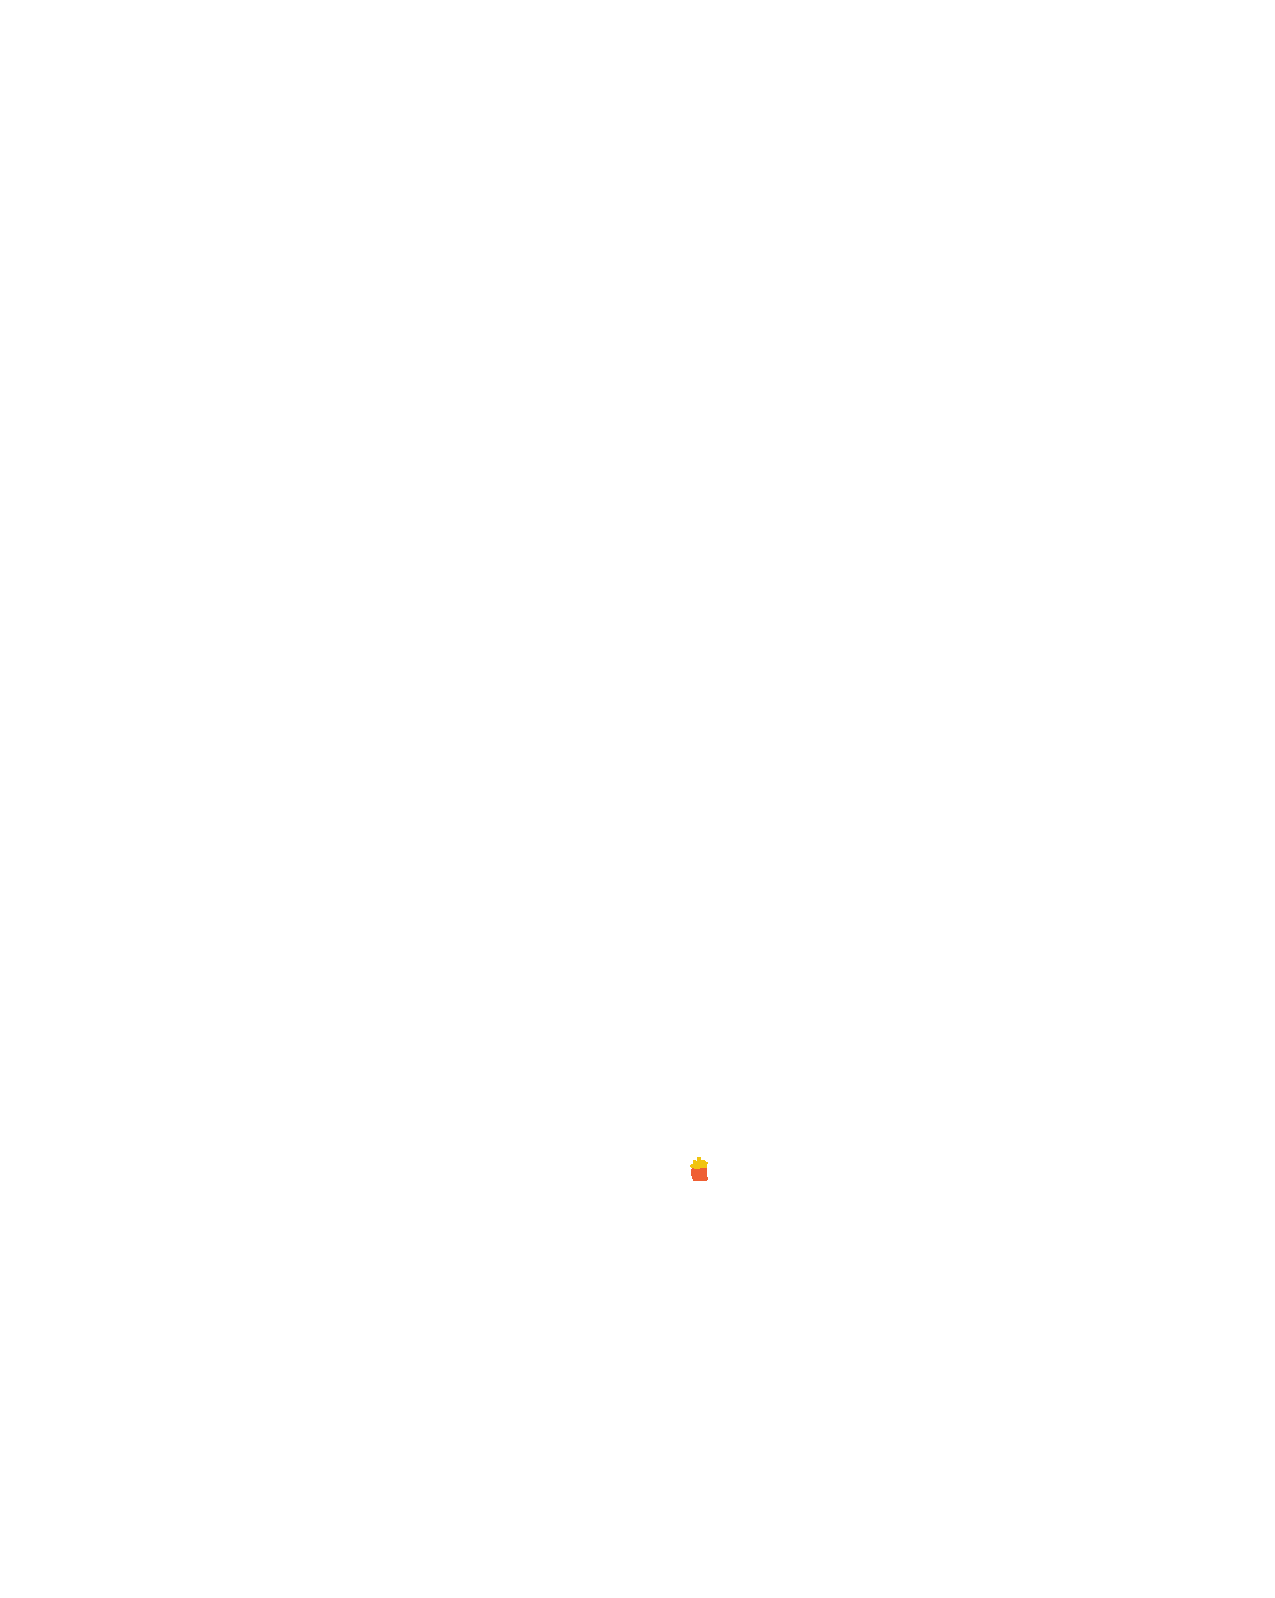
\includegraphics[width=1.5em]{figures/basis_food_icon_fries.pdf}} 
    &
    \eqfig{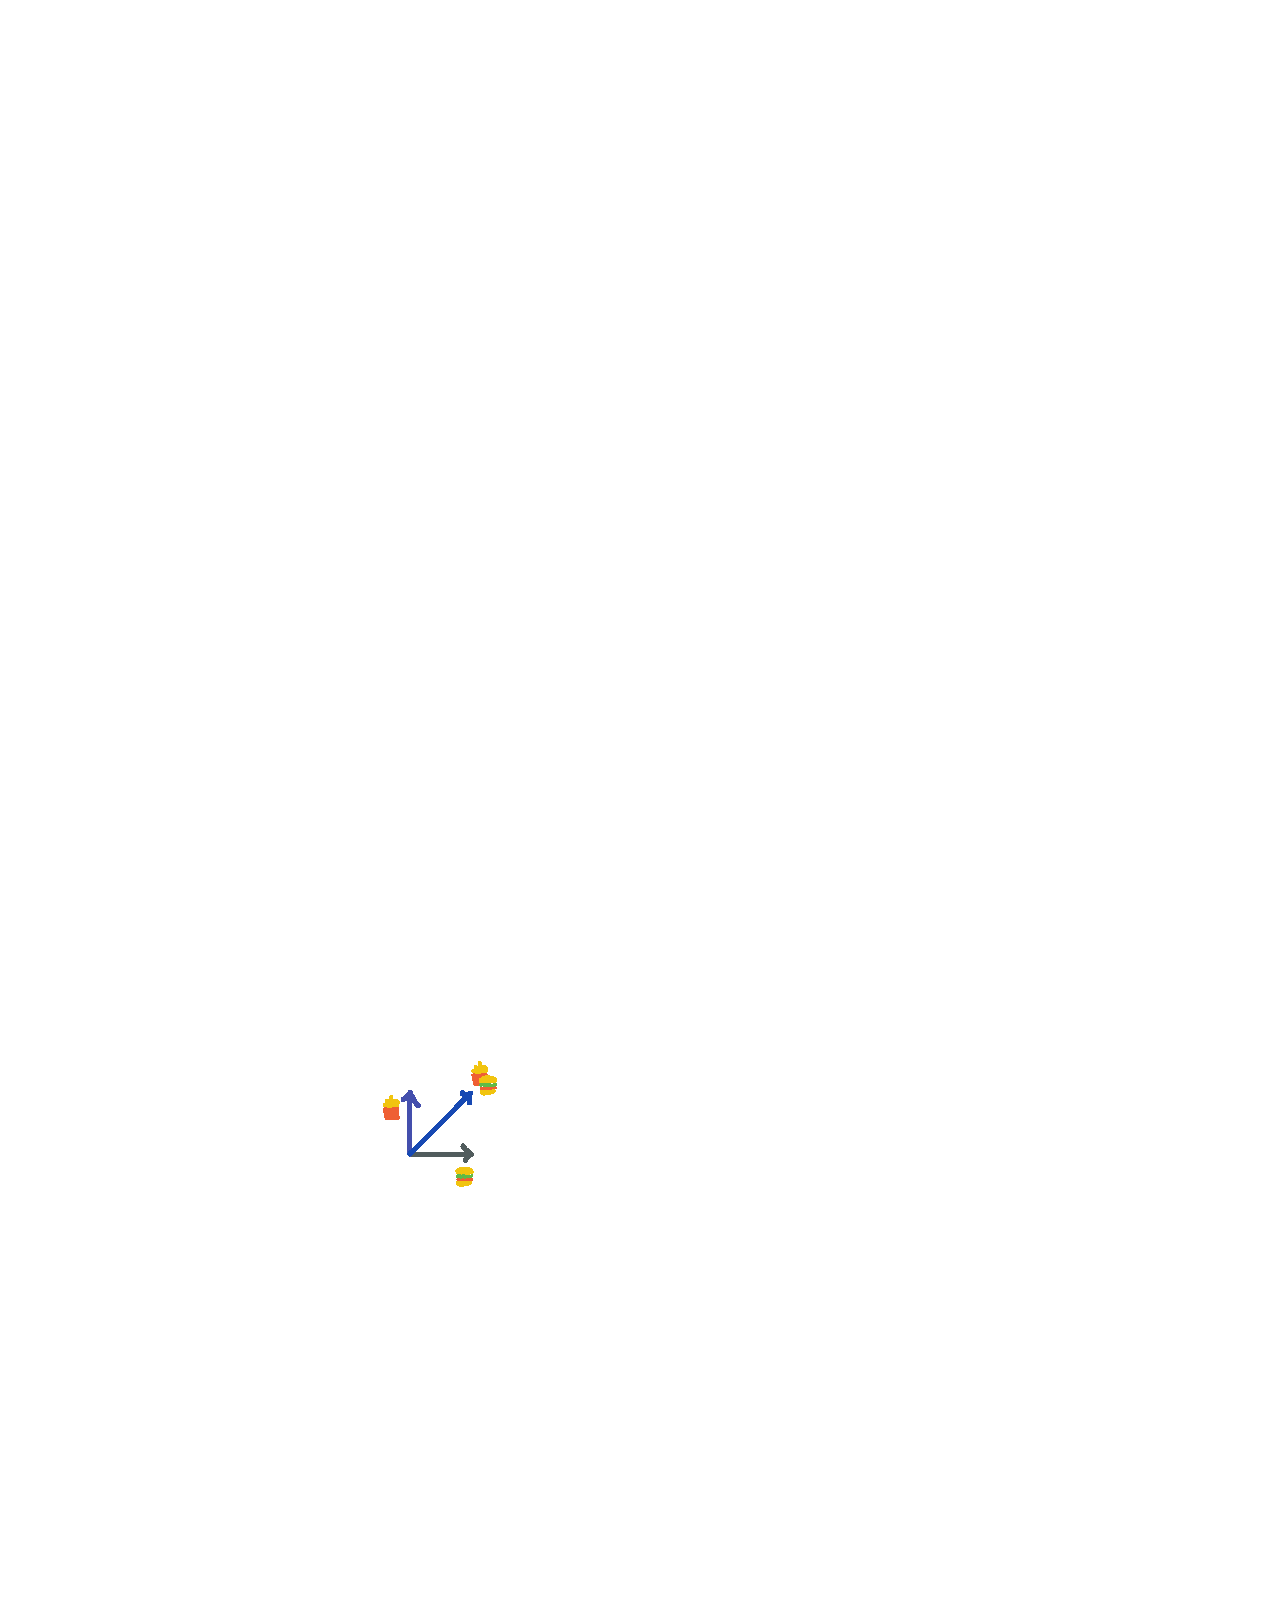
\includegraphics[width=5em]{figures/basis_food.pdf}} 
    \ .
\end{align}
Now an order $\vec{v}$ of two burgers and 1 fries is
\begin{align} 
    \vec{v} &=
    2\bas{f}_1 - \bas{f}_2 = 
    2\eqfig{
\includegraphics[width=1.5em]{figures/basis_food_icon_meal.pdf}}
    -
    \eqfig{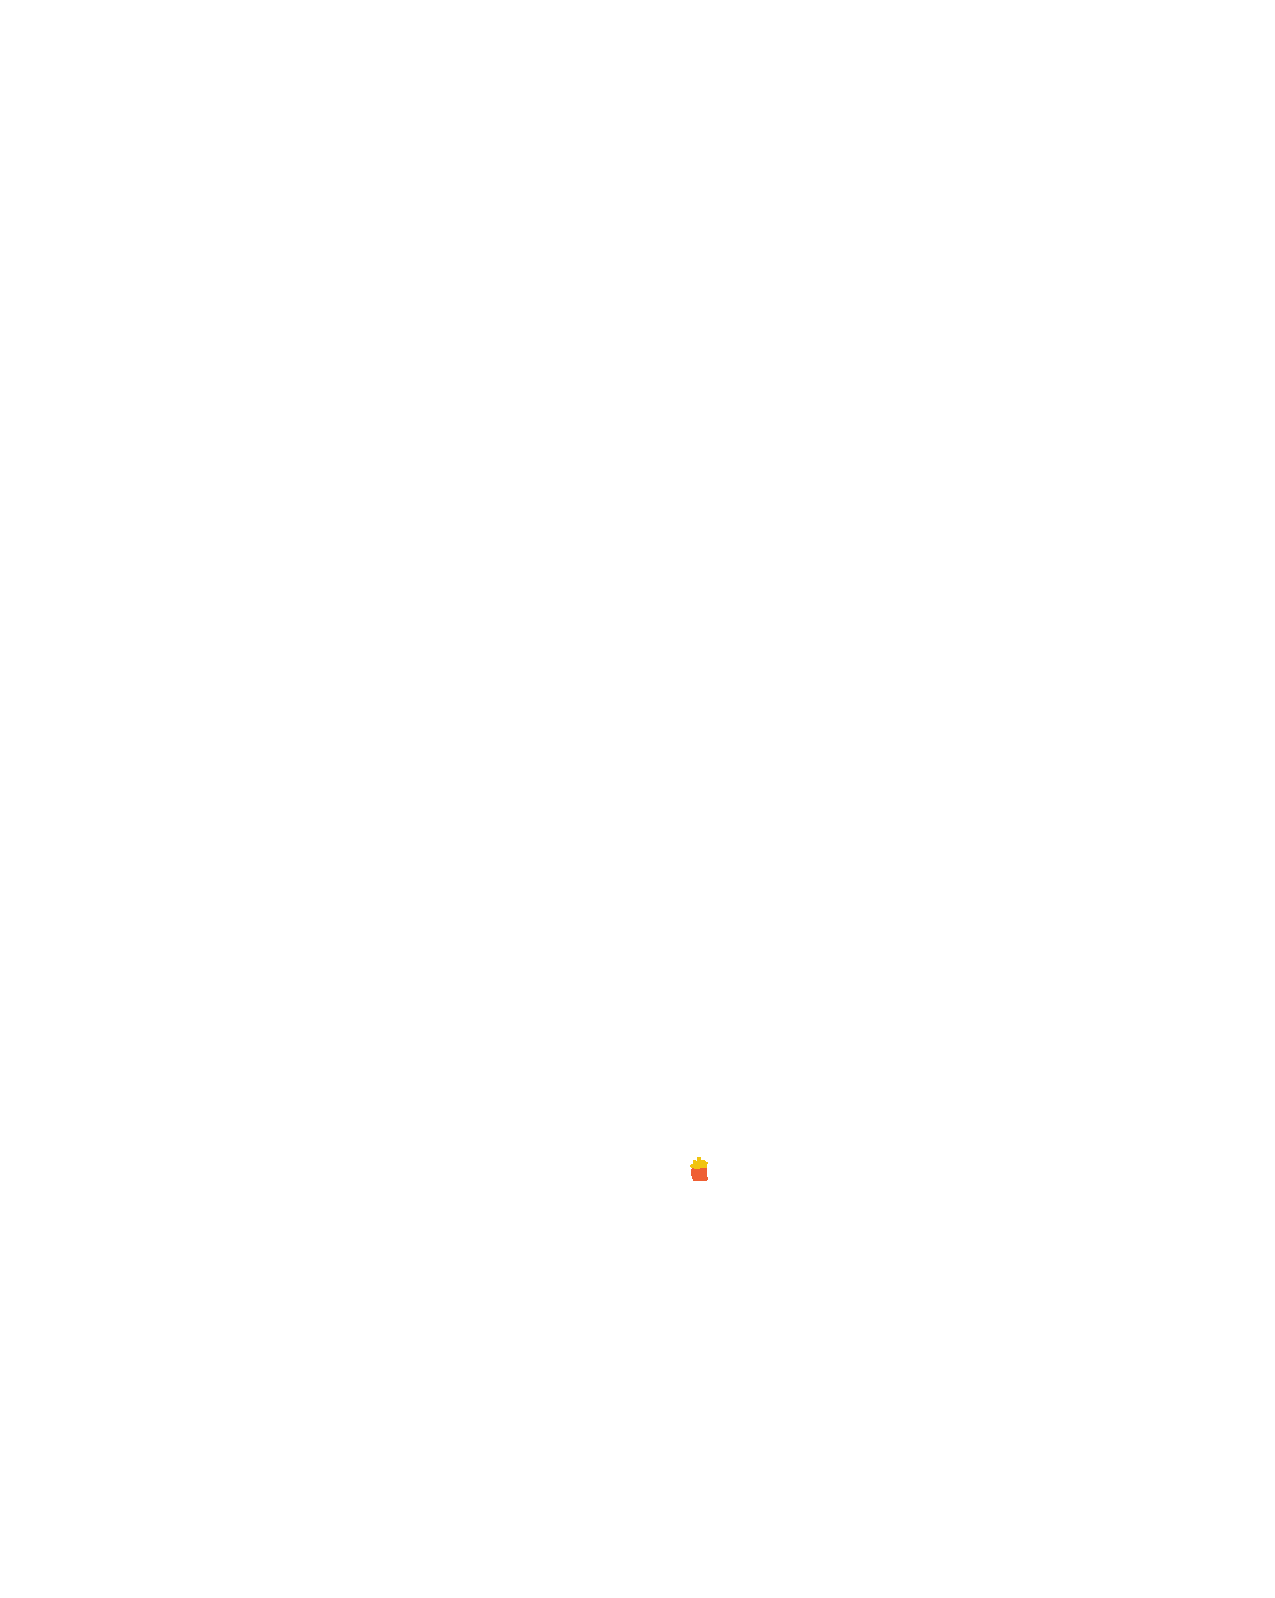
\includegraphics[width=1.5em]{figures/basis_food_icon_fries.pdf}} \ .
    \label{eq:basis:eg:meal:2}
\end{align}
We could also draw these as arrows. It would look something like this:
\begin{center}
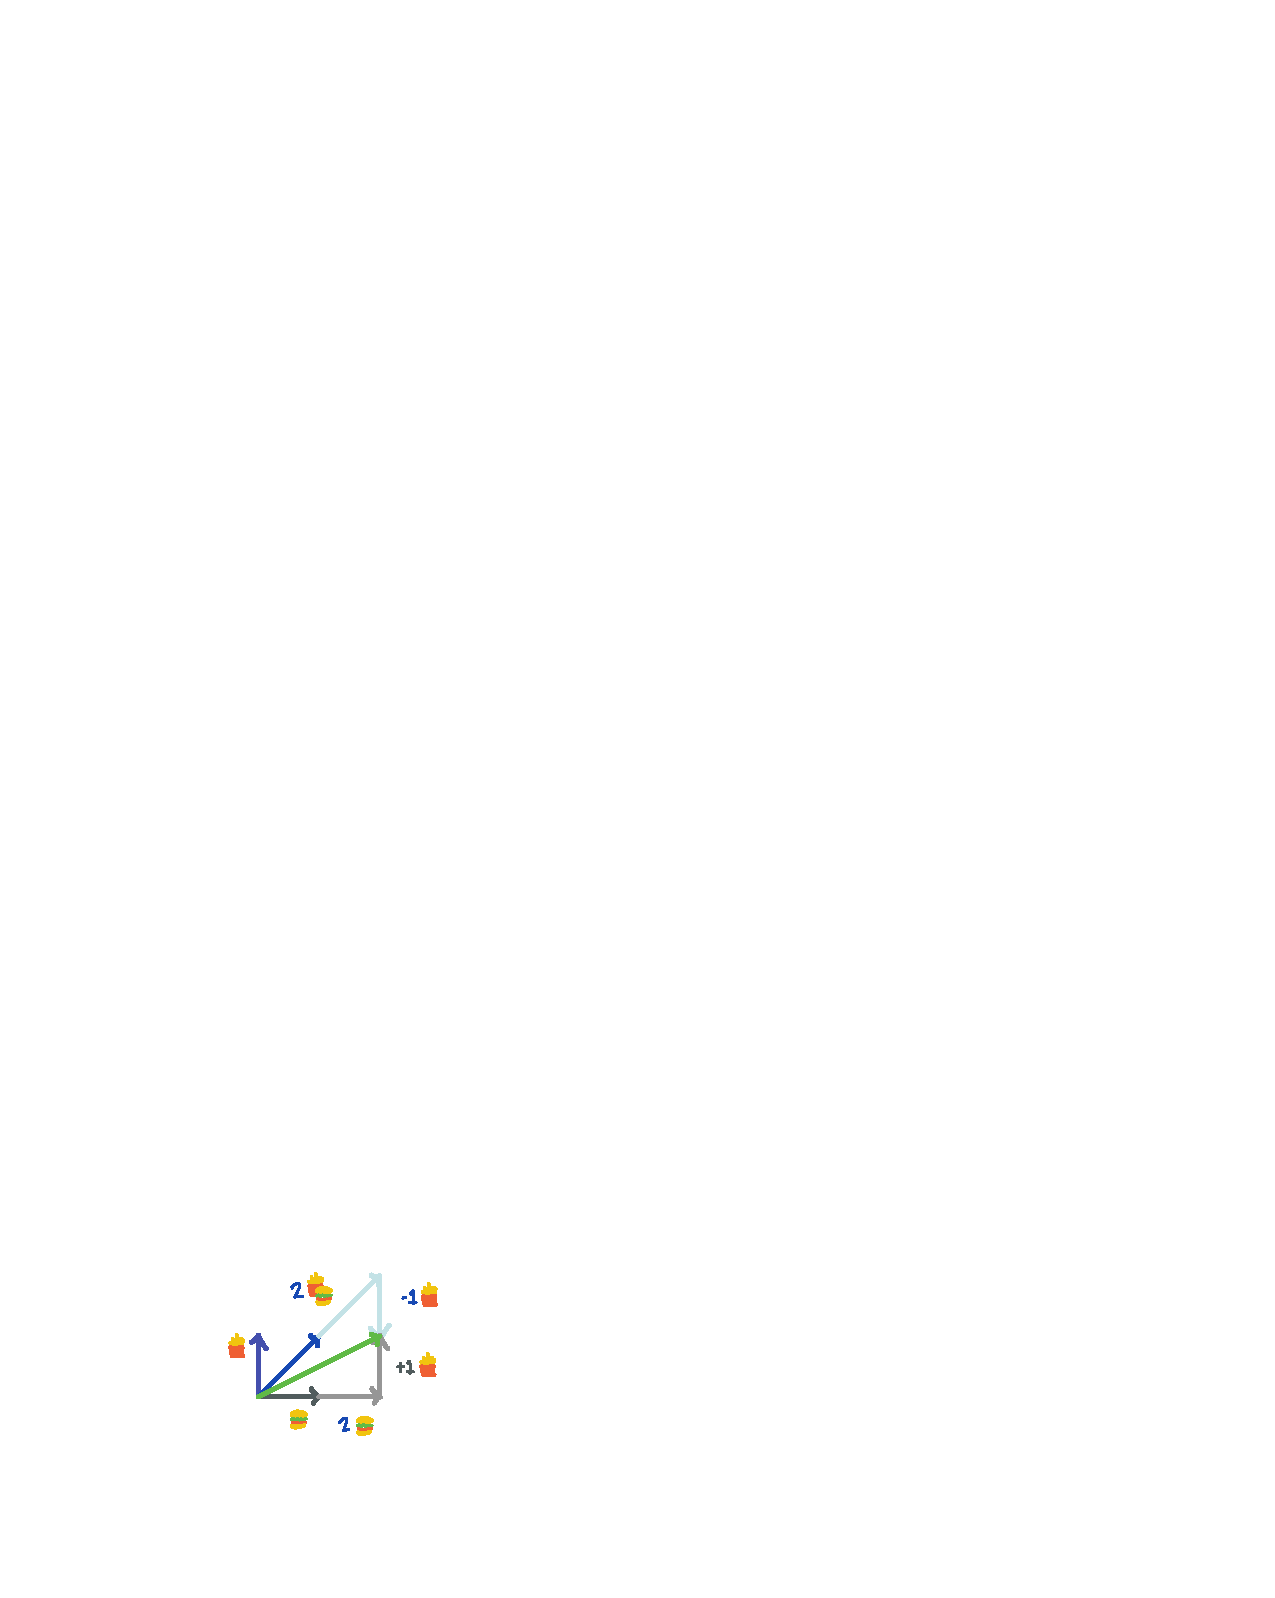
\includegraphics[width=.3\textwidth]{figures/basis_food_eg.pdf}
\end{center}
At this point, you could ask what a \emph{negative} order of fries ($-\bas{f}_2$) means. \emph{I don't know!} Maybe it means I should make fries for the cook? Maybe it means that fast food orders are not described well by vector spaces since the additive inverse may not have a clear meaning. But we have at least we are not talking about columns of numbers.
\end{example}


To make this concrete, please go through Exercise~\ref{ex:fibonacci:space} to meet a somewhat unusual vector space.
\begin{exercise}[Fibonacci sequence space]\label{ex:fibonacci:space}
One of my favorite examples of a vector space is the space of Fibonacci sequences. Fibonacci sequences are infinite lists of numbers $a_i$ that satisfy $a_{i+2} = a_i+a_{i+1}$. Once you specify the first two numbers $a_0$ and $a_1$, you can iteratively generate every other number in the sequence. Each sequence is a vector in the space of possible Fibonacci sequences. Show that this is true by confirming that a linear combination of Fibonacci sequences with each $i^\text{th}$ term added, e.g.\ $(a+b)^i = a_i+b_i$ is also a Fibonacci sequence. Give an example of a basis for the Fibonacci sequences. What is the dimension of the Fibonacci sequence space? \emph{Answer}: the dimension is two, even though each element is an infinitely long list of numbers.
\end{exercise}
\begin{marginfigure}%[th]
    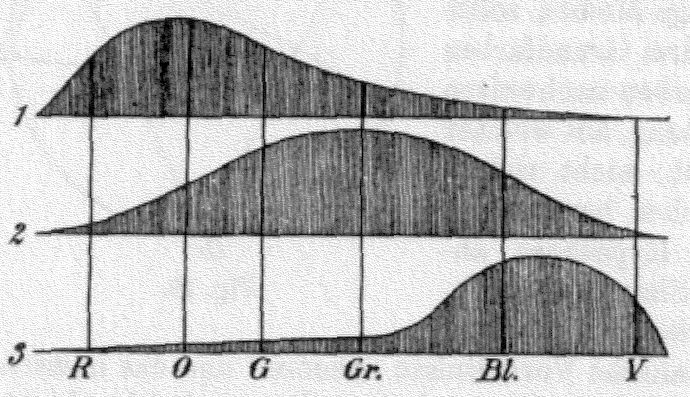
\includegraphics[width=\textwidth]{figures/YoungHelm.jpg}
    \captionsetup{font={scriptsize,sf}}
    \caption{Sketch of Young and Hemholtz (yes, the physicists) spectral sensitivities for different photoreceptors in their trichromatic color space theory. Image from Wikipedia, `Young-Hemholtz theory.'}
    \label{fig:young:hemholtz}
\end{marginfigure}
\begin{example}[Color space]\label{eg:color:space} is a vector space that highlights this idea of a more abstract basis vector. In color theory, all colors are linear combinations of red, green, and blue. This should sound really weird because in physics these colors are simply wavelengths of light: what is special about them? Nothing in nature. What is special is that our eyes have three types of color receptor cells, see Figure~\ref{fig:young:hemholtz}.\footnote{Animals can have different number of color receptor cells. One great place to read about this is Ed Yong's book, \emph{An Immense World}. Color space for those animals has a different dimension than ours.} Each type is sensitive to a certain window of the visible spectrum. We call these human eye responses the colors red, green, and blue. When we add colors, what we really mean is we're adding ``responses'' to a particular spectrum of light. When we add colors, we are not adding electromagnetic waves: we are adding neurological responses. For each type of color-sensitive cell, one `blip' of neural response is a basis vector for our color response. The sensation of a particular color is a linear combination of this basis. An actual human being is not sensitive to the whole vector space: for example, we cannot add negative colors to our sensory response. This is a fascinating subject and a surprising application of linear algebra.\footnote{There are some great YouTube videos on this. Here are a few: \url{https://www.youtube.com/watch?v=xAoljeRJ3lU}, \url{https://www.youtube.com/watch?v=AS1OHMW873s}, \url{https://www.youtube.com/watch?v=99v96TL-tuY}.} The sense in which a color is an overlap integral of a cell's sensitivity to different frequencies of light times the distribution of photons over frequency happens to also be a precursor to the inner product on infinite dimensional spaces.
\end{example}



\subsection{Changing basis} 
\label{sec:sub:basis:changing}

We started this section off by saying that the two of us just agreed on some set of basis vectors. Maybe we do not agree on a set of basis vectors. Maybe I am a little weird and I choose a set of basis vectors that seem very strange to you; this very strange basis does \emph{not} have to be aligned in any particular way.\sidenote{If you are about to say the word \emph{orthonormal}, then stop right there. We do not yet have the mathematical machinery to define orthogonality or normality.} 

\paragraph{A very silly basis}
Here is my silly choice of basis. To help us be very careful, I use square brackets for the components that \emph{you} would measure using \emph{your} basis. 
\begin{align}
    \bas{f}_1 &=
    \begin{bmatrix}
        3 \\ 1
    \end{bmatrix}
    &
    \bas{f}_2 &=
    \begin{bmatrix}
        2 \\ 2
    \end{bmatrix} \ .
\end{align}
All of my vectors are defined with respect to my basis. In fact, all the above line means is
\begin{align}
    \bas{f}_1 &= 3\bas{e}_1 + \bas{e}_2
    &
    \bas{f}_2 &= 2\bas{e}_2 + 2\bas{e}_2
    \ .
    \label{eq:change:basis:eg:1}
\end{align}
We can write this even more succinctly using tensors:
\begin{align}
    \bas{f}_i &= \bas{e}_j T\aij{j}{i} \ .
    \label{eq:change:basis:eg:2}
\end{align}
\begin{exercise}
What are the components of $T\aij{j}{i}$? \textsc{Partial answer:} $T\aij{1}{2} = 2$.
\end{exercise}


I can define a vector $\vec{a}$ with components $\alpha^{1,2}$ and package the components into a column with round brackets:
\begin{align}
    \vec{a} 
    = \begin{pmatrix}
        \alpha^1 \\ \alpha^2
    \end{pmatrix}
    =
    \alpha^i \bas{f}_i  \ .
\end{align}
What does this mean \emph{to you?} To figure this out, you would just insert the conversion \eqref{eq:change:basis:eg:1}:
\begin{align}
    \vec{a} = \alpha^i \bas{f}_i = \alpha^i T\aij{j}{i} \bas{e}_j = (\alpha^i T\aij{j}{i})\bas{e}_j \equiv \beta^j \bas{e}_j \ .
\end{align}
From this we find that the components of the vector $\vec{a}$ in your $\bas{e}_i$ basis are
\begin{align}
    \beta^j = \alpha^i T\aij{j}{i} \ . 
    \label{eq:beta:alpha:T:convert}
\end{align}
\begin{exercise}
Explicitly write out the $\beta^j$. \textsc{Partial answer:} $\beta^1 = 3\alpha^1 + 2\alpha^2$.
\end{exercise}


If I told you that I have a vector whose components---in my $\bas{f}$ basis---are
\begin{align}
    \alpha^1 &= 2 & \alpha^2 &= 3    
\end{align}
the you would understand that
\begin{align}
    \vec{a} 
    = \begin{pmatrix}
        \alpha^1 \\ \alpha^2
    \end{pmatrix}
    =
        \alpha^i \bas{f}_i 
        =
        2
    \begin{bmatrix}
        3 \\ 1
    \end{bmatrix}
    +
    3
    \begin{bmatrix}
        2 \\ 2
    \end{bmatrix}
    =
    \begin{bmatrix}
        12 \\
        8
    \end{bmatrix} 
    \equiv
    \begin{bmatrix}
        \beta^1 \\
        \beta^2
    \end{bmatrix}
    \ .
\end{align}
\begin{exercise}
Verify that these values of $\alpha^i$ and $\beta^i$ satisfy \eqref{eq:beta:alpha:T:convert}.
\end{exercise}
I am being \emph{very} careful here to distinguish between round and square brackets.
In tern, we must be \emph{very} careful in how we interpret this! The round brackets and the square brackets\sidenote{I just made up this notation for illustrative purposes.} are totally different objects. So the following statement is true:
\begin{align}
    \vec{a} = \begin{pmatrix}
        2 \\ 3
    \end{pmatrix}
    = 
    \begin{bmatrix}
        12 \\ 8
    \end{bmatrix} \ .
\end{align}
There is no paradox here: the column in round brackets are the components in the $\bas{f}$ basis while the column in square brackets are the components in the $\bas{e}$ basis. 


\paragraph{General discussion} The square and round bracket notation is somewhat cumbersome and non-standard. Instead, let us propose a notation that is just as cumbersome but more transparent:
\begin{align}
    \begin{pmatrix}
        \alpha^1\\
        \alpha^2\\
        \vdots
    \end{pmatrix}_{\bas{f}}
    &= \alpha^i \bas{f}_i
    &
    \begin{pmatrix}
        \beta^1\\
        \beta^2\\
        \vdots
    \end{pmatrix}_{\bas{e}}
    &= \beta^i \bas{e}_i \ .
\end{align}
A key idea is to see how we convert between bases.\sidenote{The plural of basis is \emph{bases} and is pronounced `bay-sees.' As a linguistic excursion, you can look up the plural of `hippopotamus.'}
\begin{align}
    \bas{f}_i = T\aij{j}{i} \bas{e}_j \ .
    \label{eq:change:of:basis:matrix:1}
\end{align}
We see that in the $\bas{e}$ basis,
\begin{align}
    \bas{f}_1 &=
    \begin{pmatrix}
        T\aij{1}{1}
        \\
        T\aij{2}{1}
        \\
        \vdots
    \end{pmatrix}_{\bas{e}}
\end{align}
and more generally,
\begin{align}
    \bas{f}_i &=
    \begin{pmatrix}
        T\aij{1}{i}
        \\
        T\aij{2}{i}
        \\
        \vdots
    \end{pmatrix}_{\bas{e}} \ .
\end{align}
And so we find the following rule.
\begin{newrule}[Change of basis matrix]\label{rule:change:of:basis:matrix}
Let $T\aij{i}{j}$ be the change of basis matrix defined by \eqref{eq:change:of:basis:matrix:1}. Then  the \emph{columns} of the matrix representation of $T\aij{i}{j}$ with the components of the $\bas{f}$ basis vectors written in the $\bas{e}$ basis:
\begin{align}
    \begin{pmatrix}
        T\aij{1}{1} & T\aij{1}{2} & \cdots \\
        T\aij{2}{1} & T\aij{2}{2} & \cdots \\
        \vdots & \vdots &\ddots  
    \end{pmatrix}
    &
    =
    \begin{pmatrix}
        | & | & \cdots \\
        \bas{f}_1 & \bas{f}_2 & \cdots \\
        | & | & \ddots 
    \end{pmatrix} \ .
\end{align}
\end{newrule}
Now let me take a moment to throw up swaths of caution tape here. The reason why the components of $\bas{f}_i$ in the $\bas{e}$ basis are given by the \emph{columns} of $T\aij{i}{j}$ has to do with our choice of how $T\aij{i}{j}$ is defined in \eqref{eq:change:of:basis:matrix:1}. In our strict index convention, \eqref{eq:change:of:basis:matrix:1} is the \emph{only} structure that makes sense.\sidenote{You could have defined a tensor $S_i^{\phantom{i}j}$ such that $\bas{f}_i = S_i^{\phantom{i}j} \bas{e}_j$, but we can equivalently define a matrix $T\aij{j}{i} = S_i^{\phantom{i}j}$ that does the same thing. If you are thinking about saying $S$ and $T$ transposes of each other---hold your horses! We do not yet have the machinery to define this.} 

We could then ask a separate question: if we know the components of a vector in the $\bas{e}$ basis, $\beta^i$, what are the components in the $\bas{f}$ basis? Then we can take \eqref{eq:change:of:basis:matrix:1} and act on both sides with the inverse transformation $(T\inv)\aij{i}{k}$
\begin{align}
    (T\inv)\aij{i}{k}T\aij{j}{i}\bas{e}_j &= (T\inv)\aij{i}{k}\bas{f}_i \\
    \delta^j_k \bas{e}_j &= (T\inv)\aij{i}{k}\bas{f}_i\\
    \bas{e}_k &=(T\inv)\aij{i}{k}\bas{f}_i \ ,
    \label{eq:intermediate:e:Tinv:f}
\end{align}
Where we use the Kronecker-$\delta$ from \eqref{eq:kronecker:delta}.
% 
Contracting both sides \eqref{eq:intermediate:e:Tinv:f} by the $\bas{e}$ basis components $\beta^k$ then gives an expression for the $\alpha^k$ components in the $\bas{f}$ basis:
\begin{align}
   \beta^k \bas{e}_k &=(T\inv)\aij{i}{k} \beta^k \bas{f}_i \equiv \alpha^i \bas{f}_i \ .
\end{align}
In other words,
\begin{align}
    \alpha^i = (T\inv)\aij{i}{k} \beta^k \ .
\end{align}
Of course, at this point you can wonder about what to do if $T$ is \emph{not} an invertible matrix---and under what conditions would that be the case? Evidently we should put some thought into what a `good' basis might be, and part of that definition is likely to involve the invertibility of the transformation between different `good' bases.

\begin{bigidea}\label{idea:2d:chart}
In physics, a choice of basis often corresponds to a reference frame. For example, we could imagine trying to look at a paper map\footnote{In ancient times maps used to be printed on large pieces of paper that were folded up. Ancient navigators would find shared community in trying to re-fold these maps so that they might fit back into their glove compartments.} while standing in Parking Lot 13 at \acro{UC R}iverside. There is a two dimensional vector space of directions from where we are standing. A natural basis is 
\begin{align}
    \bas{e}_1 &= \text{step forward}\\
    \bas{e}_2 &= \text{step to the right} \ .
\end{align}
Taking a two steps to the left would be $-2\bas{e}_2$. Then I could use my map and tell you that the Physics department is located\footnote{Nevermind that `position vectors' are not a sensible thing. As an exercise, you can try to rephrase this example in terms of velocities. It gets clunky: you are trying to throw a football with some velocity so that it reaches the physics department in a certain fixed amount of time. Analogies are like undergrads... \url{https://phdcomics.com/comics/archive.php?comicid=439}} at $900\bas{e}_1$. This is only correct if my $\bas{e}_1$ basis vector is pointing east; that is, if I am facing east. If you happen to be facing north-east, then your basis vectors would be oriented differently. Perhaps $\bas{f}_1$ still means a `step forward,' but now it is a step in the north-east direction.

We want to be able to describe physical situations in different orientations. It is often easier to describe a problem in a different frame. For example, the frame where the angular momentum (pseudo-)vector is pointed in the $z$ direction, or where the moment of inertia tensor is diagonal. In relativity, it is usually helpful to be able to boost to the rest frame of a moving body.

A more sophisticated version of a change of basis is the description of a quantum particle using its position versus its momentum. Some problems are much easier to solve if you describe the particle in terms of its momentum, while others are easier if you use position. One of the curiosities of quantum mechanics is that these two descriptions turn out to be incompatible, as manifested in the Heisenberg uncertainty relations.

All this is to say that yes: changing basis is a big $\bas{f}$'ing deal.\footnote{To paraphrase a former vice president.}
\end{bigidea}



\subsection{Goldilocks dimension} % Why isn't the modern telling called ``Karen and the three bears?''

Recall from \eqref{eq:linear:combination:looks:like:basis} that the span of a set of vectors $\vec{v}_1, \cdots, \vec{v}_N$ is the vector space $V$ of all linear combinations of those vectors. This makes us want to identify those vectors as a basis for $V$. \emph{Not so fast}. For any vector space $V$, there is a `correct' number of basis vectors vectors called the \textbf{dimension}\index{dimension} of $V$, or $\text{dim}\,V$. This dimension is the minimum number of good basis vectors that you need to describe any vector in $V$. To write it technically, $\text{dim}\,V$ is the smallest counting number $d$ such that
\begin{align}
    \forall \vec{v} \in V :\; \vec{v} = v^1 \bas{e}_1 + \cdots + v^{d}\bas{e}_{d} \ .
\end{align}
The symbol $\forall$ means ``for all,'' so the above line says: for all (really: for \emph{any}) vector $\vec{v}$ in the vector space, $\vec{v}$ is a linear combination of $d$ basis vectors. The dimension of $V$ is the smallest number $d$ for which this is true. 

If your number of proposed basis vectors is larger than this dimension then vectors do not have a unique expansion. If your number of proposed basis vectors is smaller than this dimension, then there are vectors in $V$ that \emph{cannot} be described by linear combinations of your basis vectors. And even if your number of proposed basis vectors is \emph{just right} and exactly equal to $\text{dim}\,V$, you could \emph{still} fail because some of your basis vectors are actually combinations of other basis vectors. Let us go through these cases sequentially.

\subsubsection{Too many basis vectors}

Start with the following example:
\begin{example}
Suppose you have the following proposed basis:
\begin{align}
    \bas{e}_1 &=
    \begin{pmatrix}
        1\\
        1
    \end{pmatrix}
    &
    \bas{e}_2 &=
    \begin{pmatrix}
        2\\
        1
    \end{pmatrix}
    &
    \bas{e}_3 &=
    \begin{pmatrix}
        -1\\
        \pp 1
    \end{pmatrix} \ .
    \label{eq:eg:too:many:basis:vectors:basis}
\end{align}
Suppose I then give you the vector
\begin{align}
    \vec{v} &=
    \begin{pmatrix}
        3 \\ 1
    \end{pmatrix} \ .
\end{align}
What is the linear combination of your basis vectors that produces $\vec{v}$? In other words, what are the $v^i$ so that
\begin{align}
    \vec{v}= v^i \bas{e}_i \, ?
\end{align}
You can write this as a system of equations. One solution is
\begin{align}
    \vec{v} &= -1\bas{e}_1 + 3\bas{e}_2 + 0\,\bas{e}_3 
    &
    \begin{pmatrix}
        v^1 \\ v^2 \\ v^3
    \end{pmatrix}
    =
    \begin{pmatrix}
        -1 \\ \pp 3 \\ \pp 0
    \end{pmatrix} \ .
\end{align}
Great, problem solved, right? Not quite. We could have \emph{alternatively} written
\begin{align}
    \vec{v} &= 0\,\bas{e}_1 + \frac{4}{3}\bas{e}_2 - \frac{1}{3}\bas{e}_3 
    &
    \begin{pmatrix}
        v^1 \\ v^2 \\ v^3
    \end{pmatrix}
    =
    \begin{pmatrix}
        \pp 0 \\ \pp 4/3 \\ - 1/3
    \end{pmatrix} \ .
\end{align}
Now we should be concerned. For the \emph{same} basis, there are at least \emph{two} different sets of coefficients that describe the \emph{same} vector! How are we supposed to keep track of the fact that there are \emph{degeneracies} where different combinations of components $v^i$ actually mean the \emph{same} vector? That would be madness.\sidenotemark
\end{example}\sidenotetext{This is absolutely silly to do, but it turns out there are cases in physics where we make use of this type of madness. These are called \emph{gauge theories}. An example of a gauge theory is electromagnetism, where there is a redundancy that we call a \emph{gauge symmetry}. This corresponds to the fact that many different choices of gauge potential (the electric and vector potentials) produce the same physical electric and magnetic fields. An excellent introduction to this idea is \arXiv{hep-th/0611201}.}
\begin{exercise}
Write out and solve the system of equations from the previous example. Show that there are an infinite number of solutions. In fact, these solutions are a line in a three-dimensional space.
\end{exercise}

Evidently you can have \emph{too many} basis vectors. In the above example, we could have taken any two of the three basis vectors and still described the same vector space. That vector space thus has dimension two. We can see that one manifestation of the fact that we had too many basis vectors that we had more components $v^i$ than the dimension of the space.\sidenote{Indeed, the fact that the basis vectors themselves could be written with only two components with respect to the canonical basis tells us we are doing something silly with \emph{three} basis vectors.}

So if you have too many basis vectors, there is no unique way of assigning vector components $v^i$ to a vector $\vec{v}$. We do not want to have too many basis vectors. 


\subsubsection{Too few basis vectors}

Let us see what happens if we go the other way. 
\begin{example}
Suppose you have the following proposed basis:
\begin{align}
    \bas{e}_1 &=
    \begin{pmatrix}
        1\\
        1\\
        0
    \end{pmatrix}
    &
    \bas{e}_2 &=
    \begin{pmatrix}
        \pp 1\\
        -1\\
        0
    \end{pmatrix}
    \ .
    \label{eq:eg:too:few:basis:vectors:basis}
\end{align}
Suppose I then give you the vector
\begin{align}
    \vec{v} &=
    \begin{pmatrix}
        3 \\ 1 \\ 1
    \end{pmatrix} \ .
\end{align}
What is the linear combination of your basis vectors that produces $\vec{v}$? Once again, we solve the component-wise system of equations 
\begin{align}
    \vec{v}= v^i \bas{e}_i \, ,
\end{align}
where we recognize that there is only a sum over $i=1$ and $i=2$. There is \emph{no} third basis vector. We can uniquely assign coefficients to match the top two components of $\vec{v}$, but there is \emph{no} linear combination of $\bas{e}_1$ and $\bas{e}_2$ that can produce a non-zero element in the last component. Thus $\vec{v}$ is \emph{not} in the span of $\vec{e}_1$ and $\vec{e}_2$. If we want $\vec{v}$ to be part of the vector space $V$, we need to augment our basis with another basis vector.
\end{example} 
\begin{exercise}
Write out and solve the system of equations from the previous example. Show that there are more constraints than free parameters (coefficients $v^i$) and that the constraints cannot be simultaneously. Give an example of a third basis vector that would allow you to uniquely write the vector $\vec{v}$.
\end{exercise}

If you have too few basis vectors, then there seems to be more `space' than the vector space spanned by your basis. That is fine, you just have to be aware that \emph{too few basis vectors} means that this reduced set of basis vectors spans what is called a \textbf{subspace}\index{subspace}. This is the set of vectors spanned by an `incomplete' basis.\sidenote{This is all somewhat hand-wavey because as we abstract away the meaning of the basis vectors it is not always obvious when there is more `space' to be described. In Example~\ref{eg:color:space}, you could say that color space is three dimensional. Or you could say that this is a subspace of a larger color space where we imagine that humans had a fourth type of cone cell. Mantis shrimps have a 16-dimensional color space.}



\subsubsection{Just the right number of basis vectors}

Suppose you have just the right number of basis vectors. You should be all good, right? Maybe not. 
\begin{example}
The canonical basis \eqref{eq:canonical:basis} is an example of a good basis. Let us consider the case of a three-dimensional vector space spanned by the first three of these basis vectors, $\bas{e}_{1,2,3}$. Now consider the following basis:
\begin{align}
    \bas{f}_1 &=
    \begin{pmatrix}
    1 \\ 1 \\ 2  
    \end{pmatrix}_{\bas{e}}
    &
    \bas{f}_1 &=
    \begin{pmatrix}
    1 \\ 0 \\ 1  
    \end{pmatrix}_{\bas{e}}
    &
    \bas{f}_1 &=
    \begin{pmatrix}
    0 \\ 1 \\ 1  
    \end{pmatrix}_{\bas{e}} \ .
    \label{eq:eg:basis:lin:dependent}
\end{align}
Remember that the subscript $\bas{e}$ reminds us that those columns are written in the canonical basis.
You know the name of the game. If we have a vector $\vec{v}$, can you solve for the coefficients $v^i$ in the $\bas{f}$ basis:
\begin{align}
    \vec{v} = 
    \begin{pmatrix}
        2 \\ 2 \\ 3
    \end{pmatrix}
    = v^i \bas{f}_i \, ?
\end{align}
What are the coefficients/components $v^i$? It turns out that there is no solution.
\end{example}
\begin{exercise}
Write out the system of three equations for the three components $v^i$ and show that they are \emph{degenerate} and that for a general vector $\vec{v}$ in the $\bas{e}$ basis one \emph{cannot} find solutions for $v^i$. Give an example of a vector that \emph{can} be written in the $\bas{f}$ basis. Argue that vectors that can be written in the $\bas{f}$ basis form a \emph{two} dimensional subspace.
\end{exercise}

Can you see what went wrong in the $\bas{f}$ basis in the previous example? One hint is that
\begin{align}
    \bas{f}_3 = \bas{f}_2 - \bas{f}_1 \ .
\end{align}
% {eq:eg:basis:lin:dependent}
In other words: one of the basis vectors is a \emph{linear combination} of the others.\sidenote{It does not matter which one. In this example, you could pick any basis vector and write it in terms of the other two.} We say that this set of vectors is \textbf{linearly depenent}\index{linearly dependent}.  Because you can replace $\bas{f}_3$ with a linear combination, then any proposed linear combination $v^i$ of the three $\bas{f}$ basis vectors can be more simply written as a linear combination of only two basis vectors:
\begin{align}
    v^i \bas{f}_i = (v^1-v^3)\bas{f}_1 + (v^2+v^3)\bas{f}_2 \equiv w^1 \bas{f}_1 + w^2\bas{f}_2 \ .
\end{align}
On the right-hand side we show that could have otherwise written any such ``three component'' vector $v^i$ as a linear combination of two basis vectors. This means that vectors $v^i\bas{f}_i$ are actually part of a two-dimensional subspace and should properly be described by only two basis vectors. If we want to describe the entire three-dimensional space spanned by $\bas{e}_{1,2,3}$, we need a third \emph{linearly independent} basis vector. 

The example is in contrast to, say, the canonical basis, which is \textbf{linearly independent}\index{linearly independent}. There means that there no vector $\bas{e}_i$ that can be written as a linear combination
\begin{align}
    \bas{e}_1 \neq \sum_{j \neq 1} \alpha^j \bas{e}_j \ .
\end{align}
This is obvious in the canonical basis because each basis vector is only non-zero for a unique index $i$.


\begin{bigidea}[Basis]
When we say that we have a basis $\bas{f}$ for a vector space $V$, we mean that
\begin{enumerate}
    \item $\text{Span}(\bas{f}_1, \cdots \bas{f}_N) = V$. This means that any vector in $V$ can be written $\vec{v} = v^i \bas{f}_i$. If you cannot do this, then you do not have enough [independent] basis vectors.
    \item The basis vectors $\bas{f}_{1,\cdots,N}$ are each linearly independent from one another. This means that there is no basis vector that can be written as a linear combination of the other basis vectors. If this is not true, then you have too many basis vectors: at least one is linearly dependent on the others.
\end{enumerate}
These conditions are assumed when we say we have a basis. We have not said anything about what makes a \emph{good} basis, though it is clear that the canonical basis \eqref{eq:canonical:basis} is a good basis.
\end{bigidea}
You may have a sense in which basis vectors should be orthonormal. We still do not yet have the machinery to define orthonormality.s



\section{Linearity}

\begin{bigidea}[Linearity] We say that a function $f$ is \textbf{linear}\index{linear} if linear combinations of arguments (inputs) produce linear combinations of outputs. Suppose $f$ is a function that takes in some object, $\vec{x}$. The output of $f$ can be the same type of object or a different type of object. Then $f$ is linear if for any two input-type objects $\vec{x}$ and $\vec{y}$ and any two numbers $\alpha$ and $\beta$:
\begin{align}
    f(\alpha\vec{x}+ \beta\vec{y}) = \alpha f(\vec{x}) + \beta f(\vec{y}) \ .
    \label{eq:linear:function}
\end{align}
Let us suppose the inputs $\vec{x}$ and $\vec{y}$ are vectors. Then the argument on the left-hand side is a linear combination of vectors, which is itself a vector. Linearity means that if we already know what $f(\vec{x})$ and $f(\vec{y})$ are, then we do not have to recalculate anything to find $f(\alpha\vec{x}+\beta\vec{y})$; we simply take a linear combination of the outputs with the same coefficients, $\alpha$ and $\beta$.
\end{bigidea}

\begin{example}
Consider functions from $\mathbbm{R}\to\mathbbm{R}$. These are ordinary functions that take numbers and return numbers. Using our definition, $f(x) = ax$ is linear because
\begin{align}
    f(\alpha x+\beta y) = a(\alpha x + \beta y)  = a\alpha x + a \beta y =\alpha f(x) + \beta f(y) \ .
\end{align}
\end{example}

\begin{exercise}
Show that the equation for a line $f(x) = ax + b$ is \emph{not linear} for $b\neq 0$.\sidenotemark

Deduce that it is generally true that a linear function must satisfy $f(\vec{0}) = 0$. \textsc{Hint}: consider taking linear combinations with $\vec{0}$.
\end{exercise}\sidenotetext{Yes, you heard this correctly. A function that plots to a line in the Cartesian plane is not necessarily \emph{linear}.}

By the way, we often use the term \textbf{map}\index{map} instead of function. I think this is because some people assume that a function only outputs a number, whereas a `map' can take in some object and spit out another object---where the output object may have more structure than a number.\sidenote{For example, it may take in a vector and output a vector.}

\section{Linear Maps}\label{sec:linear:maps}

We may combine the idea of a vector space with our definition of linearity to sharpen some of our language. A \textbf{matrix}\index{matrix} is a linear function that takes vectors and spits out other vectors. We say that these are \emph{linear maps} from $V\to V$. Equivalently, the matrix also takes row vectors and spits out row vectors, so they are also maps from $V^* \to V^*$.  In fact, they are \emph{also} linear functions that take a vector and a row vector into a number:
\begin{align}
    M:\; V\otimes V^* \to \# \ . \label{eq:M:tensor:product}
\end{align}
The left-hand side just says ``$M$ is a map that takes...''
We have introduced the $\otimes$ \textbf{tensor product}\index{tensor product} notation.\sidenote{I'll be real honest with you: sometimes I just write this as $\times$.} The tensor product is like a `multiplication' of \emph{spaces}. 
% 
The above line simply means a linear map that takes an element of $V$ and an element of $V^*$ to produce a number.\sidenote{The $f:V\to\#$ notation does not necessarily mean that $f$ is linear. But in this course we only deal with linear functions/maps. }

This means you can think of row vectors as linear maps from vectors to numbers. In turn, vectors are linear maps that take row vectors to numbers:
\begin{align}
    \row{w}:&\; V\to \# &
    \vec{v}:&\; V^* \to \# \ .
\end{align}
In should be clear that \emph{both} of these refer to $w_iv^i$. If you know all the components of a row vector $w_i$, then I can give you \emph{any} $\vec{v}$ and you can perform the contraction $w_iv^i$ to produce a number. That means the information that you have (the components $w_i$) can be assembled---using our contraction rule---into a machine that takes any vector and spits out a number.

\begin{exercise}
What are all of the possible ways of treating a $(p,q)$ tensor as a linear function? That is: what are the possible inputs for such an object, and for each object, what is the output? For example, if $q\geq 1$, then I can feed a $(p,q)$ tensor a vector and the output is a $(p,q-1)$ tensor.
\end{exercise}

\section{Interlude: some math-speak}

\paragraph{Jargon: functions, maps, transformations} Let us get some terminology sorted out.\sidenote{This paragraph is to establish the correct mathematical jargon. Usually one can get away with being somewhat sloppy and using these terms interchangeably, but we should be clear about the distinction somewhere in these notes.}
A \textbf{function}\index{function} is a mathematical machine that takes some inputs and produces some output. The inputs can be numbers, vectors, or more sophisticated objects. The outputs may also be numbers, vectors, or more sophisticated objects. The outputs do not have to be the same type of object as the inputs---in general they are not.
% 
A \emph{function} that takes one input and returns one output is called a \textbf{map}\index{map}. 
% 
A \emph{map} that takes one type of object and returns the same type of object is called a \textbf{transformation}\index{transform}. Mathy-folks like to draw diagrams like Fig.~\ref{fig:Linear Transformation}.

\begin{figure}[tb]
\sidecaption[][-2\baselineskip]{%
        Example of a linear transformation. The transformation $M$ (for matrix) takes a vector $\vec{v}$ and turns it into a different vector that we call $\vec{v}'$. This new vector is related to $\vec{v}$ by the matrix $\vec{v'}=M\vec{v}$. \emph{Every} vector is transformed under the map $M$. This is an \emph{active transformation} where all vectors transform, but the basis (${\bas{e}}_i$) stays fixed. \label{fig:Linear Transformation}}
        %
        %% \label command inside the \sidecaption command
    \centering
    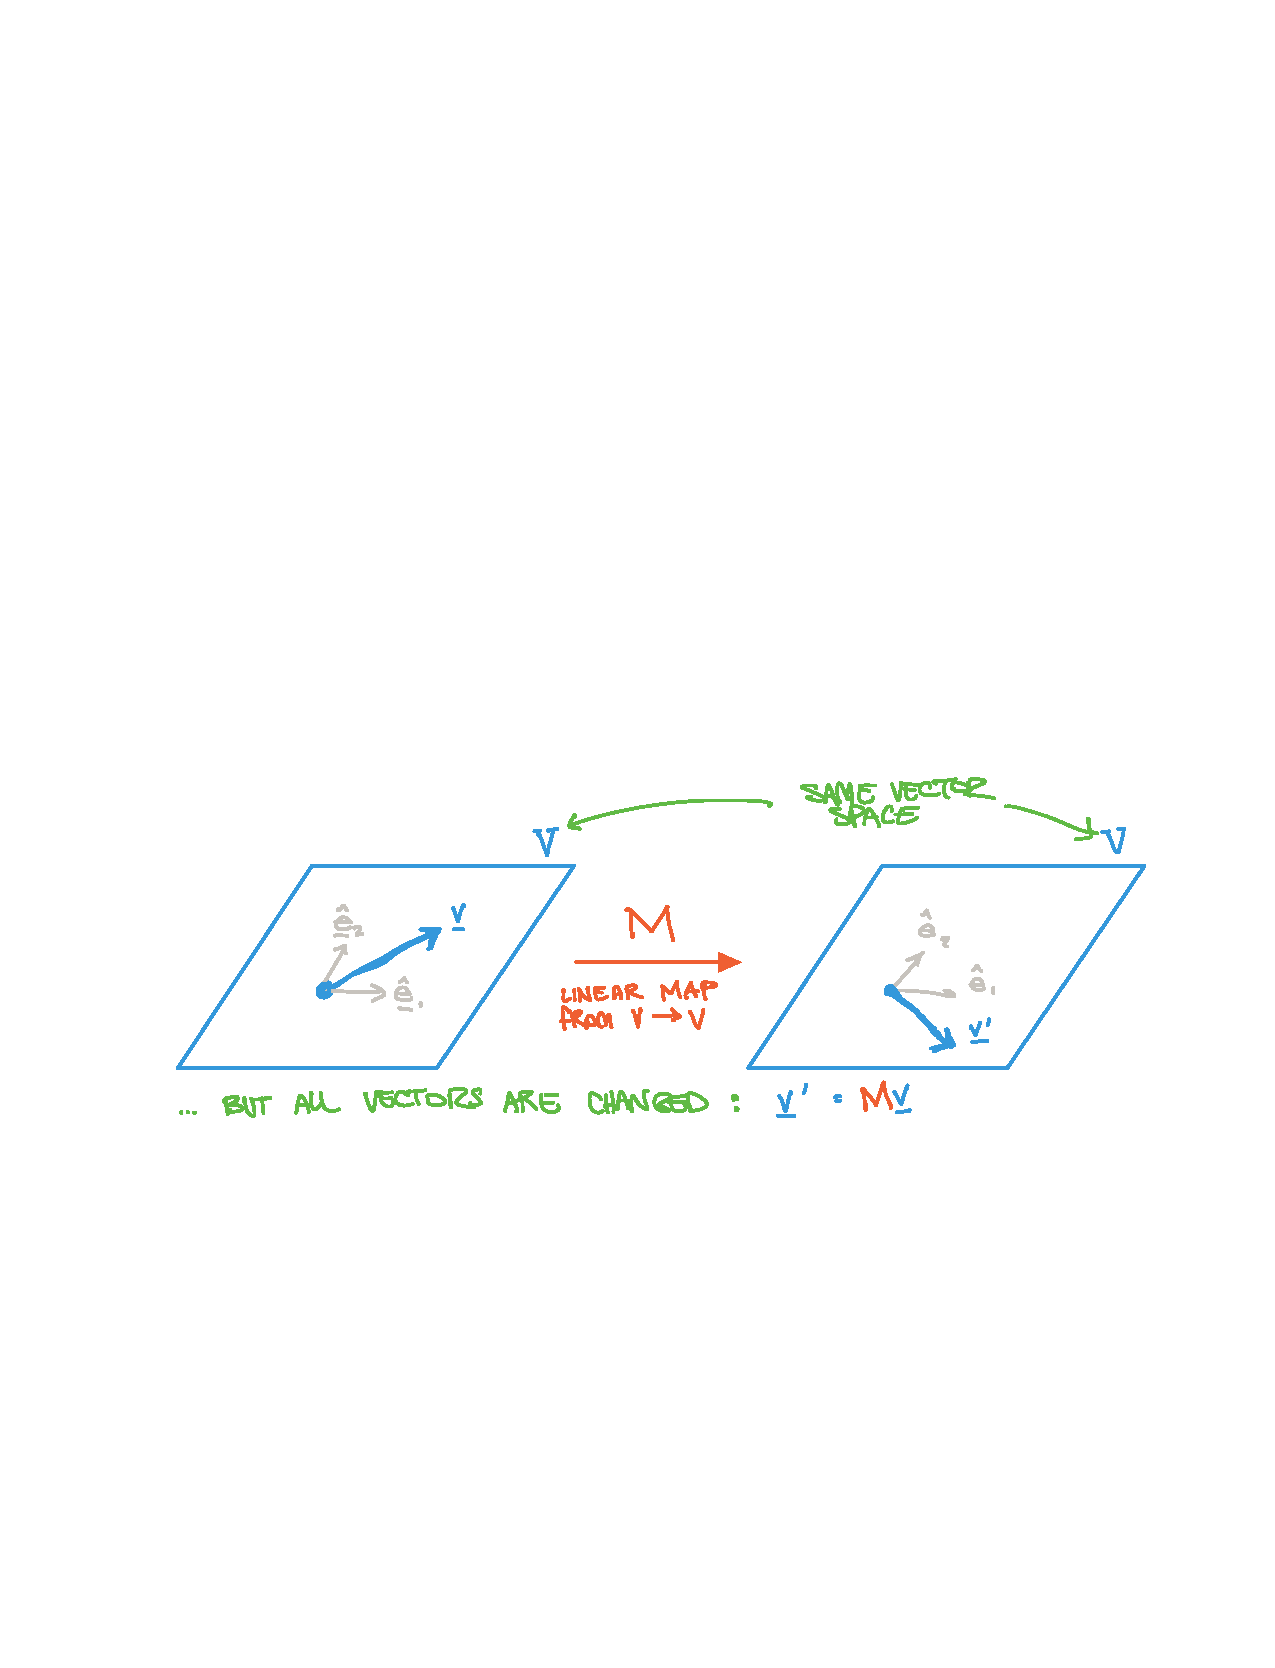
\includegraphics[width=\textwidth]{figures/lineartransformation.pdf}
\end{figure}


\begin{example}
Here are a few examples of each of the above terms:
\begin{itemize}
    \item A price checker at a store takes in barcodes and returns the cost of the item. This is a \emph{map} from barcodes to prices. This is not a map between vector spaces.\sidenotemark
    \item Conversion from kilograms to pounds is a \emph{map} takes a quantity in one unit and converts it to the same quantity in different units. This map is also \emph{linear}: if the input quantity is twice as heavy in kilograms, it will be twice as heavy in pounds. If you add two quantities in kilograms, the mass of the total object in pounds is the sum of the individual masses in pounds.
    \item A function that takes in a vector $\vec{v}\in\mathbbm{R}^2$ and returns $2\vec{v}$ is a transformation. Both the inputs and outputs are vectors in the same vector space. 
\end{itemize}
\end{example}\sidenotetext{At least I cannot figure out a reasonable vector space interpretation. I think I was already pushing it a bit far when we talked about cheeseburger-and-fries space in Example~\ref{ex:cheeseburger:space}.}

\paragraph{More jargon: one-to-one, onto, invertible}

We are going to make a big deal about \textbf{invertible transformations}\index{invertible}. An invertible transformation is one that can be reversed or undone. The transformation need not be linear---though our focus will be linear invertible functions---so for this paragraph let use write $\vec{f}(\vec{v})$ to mean an invertible, not-necessarily-linear transformation. I have even written the function as $\vec{f}$ rather than $f$ to remind us that the output is a vector. Mathematically, an invertible function is one where $\vec{f}^{-1}(\vec{v})$ is defined for any $\vec{v}$ and
\begin{align}
    \vec{f}\inv(\vec{f}(\vec{x})) = \vec{f}(\vec{f}\inv(\vec{x})) = \vec{x} \ .
\end{align}
The \emph{reason} why we care about invertible transformations is precisely the point in \bigidearef~\ref{idea:matrix:inverse:in:physics}: so much of physics is written in the form
\begin{align}
    (\text{operator})\, \ket{\text{state}} = \ket{\text{source}} \ ,
\end{align}
and our job is to invert the operator so that we can figure out what the state is as a function of the source. That is, we are usually given an equation
\begin{align}
    \vec{f}(\vec{x}) = \vec{w} \ ,
\end{align}
and we are given the form of the function $\vec{f}$ and the value of the source $\vec{w}$.\sidenote{Maxwell's equations are like this: on the left-hand side there's some fancy vector calculus differential operator acting on the field that you want to calculate, on the right-hand side there is some kind of charge or current distribution.} Our job is to determine $\vec{x} = \vec{f}\inv(\vec{v})$. 

Sometimes it is the case that $\vec{f}(\vec{x})$ is a pretty nasty function.\sidenote{By nasty I mean nonlinear. By nonlinear I mean \emph{not linear}, where the definition of linearity is \eqref{eq:linear:function}.} So instead of using $\vec{f}$, we can perform a Taylor expansion and consider the \emph{linear} part of $\vec{f}$. From our discussions so far, a linear transformation is represented as a matrix, $M$. Thus we end up writing:
\begin{align}
    \vec{f}(\vec{x}) \approx M\vec{x}  \ ,
\end{align}
and the problem inverting $\vec{f}$ reduces to the problem of inverting a linear transformation $M$. It is for this reason that we make a big deal about understanding when $M$ is invertible and, when it is, how to determine $M\inv$ in a systematic way.\sidenote{In Exercise~\ref{ex:matrix:inversino:the:hard:way} you already showed that finding the inverse of a matrix boils down to writing out and solving a system of equations. This method is intractable for very large matrices. Our goal is to reach infinite-dimensional matrices.}

\begin{example}
A function that takes your student identification number and returns your net\tacro{ID} is one-to-one. Every student identification number corresponds to a unique student with a unique net\tacro{ID}. However, not every net\tacro{ID} belongs to a student---faculty have net\tacro{ID}s but not student identification number, for example---so this function is not invertible. 
\end{example}

A few more bits of jargon. We won't use these, but consider these to be essential tools if you ever find yourself in a verbal sparring match with a mathematician:
\begin{enumerate}
    \item \textbf{Injective}\index{injective}/\textbf{one-to-one}\index{one-to-one}: 
    every output is unique; if you knew the output then you can deduce the input. However there may be some output-class objects that are not the outputs of the function for any input.
    \item \textbf{Surjective}\index{surjective}/\textbf{onto}\index{onto}: every output-class object is the result of some input, however there may be multiple inputs that produce the same output.
    \item \textbf{Bijective}\index{bijective}: this is a fancy name for \emph{invertible}. 
\end{enumerate}
% Every linear function is surjective. 

\begin{example}
Dual vectors are linear functions of vectors to numbers. Any non-zero dual vector $\row{w}$ is surjective. To see this, take any vector $\vec{v}$ and calculate $\row{w}\vec{v}$; call this number $a$. Any other number, say $b$, is the output of $\row{w}$ acting on $(b/a)\vec{v}$. Thus every output-class object (number) is realized as $\row{w}$ acting on some input. 
\end{example}

\begin{example}
In general, dual vectors are \emph{not} injective. For example, consider the dual vector $\row{w}=\begin{pmatrix}
    a & -a
\end{pmatrix}$. Then $\row{w}\vec{v} = 0$ for any vector $\vec{v}$ of the form
\begin{align}
    \vec{v} = 
    \begin{pmatrix}
        b \\ b
    \end{pmatrix}\ .
\end{align}
The zero vector is of this form so that $\row{w}\vec{0}=0$, as required by linearity. 
\end{example}


% Row vectors as 
% The fact that matrices take vectors and return vectors tells us that they enact transformations on the \emph{space} of vectors. Under the action of a matrix, every allowed vector is transformed into a different vector. 


\section{Basis in terms of linear transformations}

\begin{figure}[tb]
    \centering
    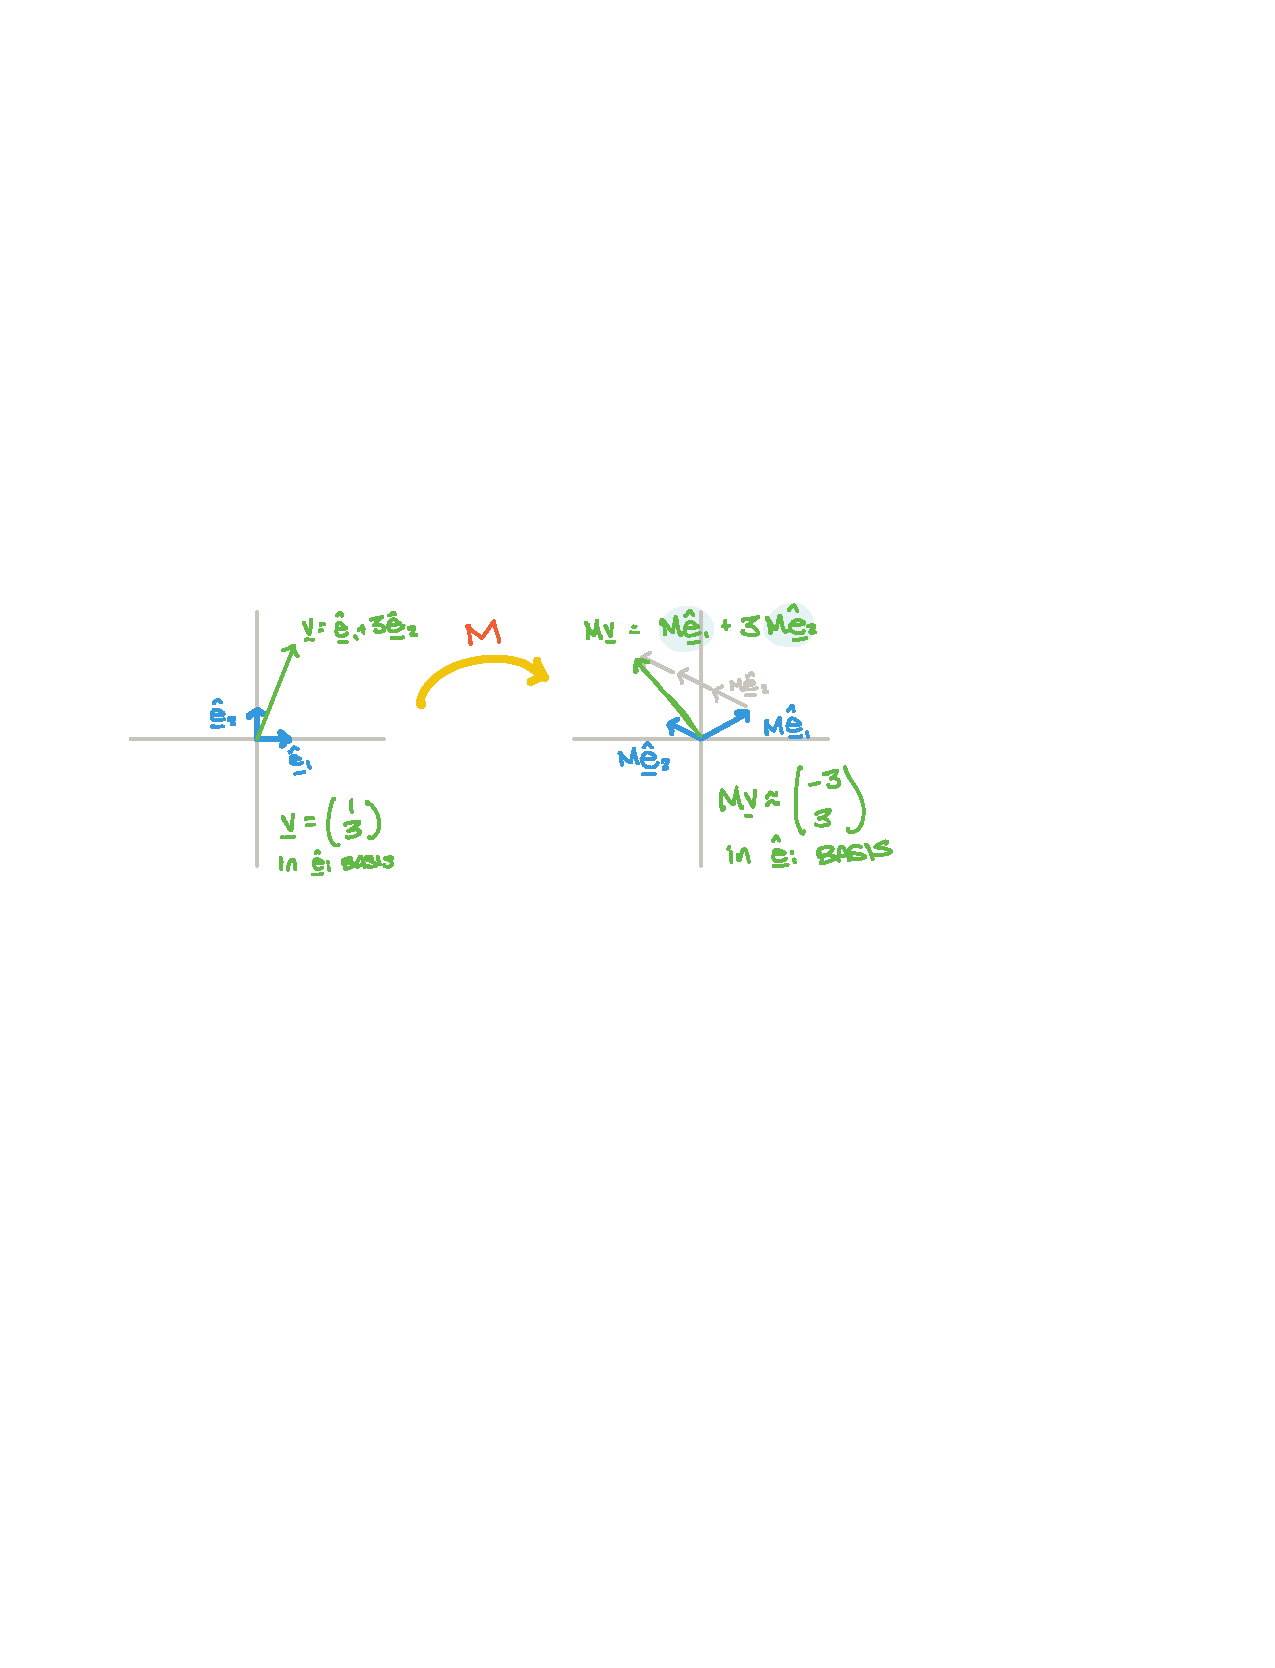
\includegraphics[width=.8\textwidth]{figures/maps_M.pdf}
    \caption{$M$ is a linear transformation from $\RR ^2\to\RR ^2$. If we know the action of $M$ on the basis vectors $\bas{e}_i$ of $\RR ^2$, then we know the action of $M$ on any vector $\vec{v}$.}
    \label{fig:map:M}
\end{figure}

The magic of linearity is that if you know how basis vectors transform, then you know how all vectors transform. This is demonstrated in Figure~\ref{fig:map:M}. In turn, we can understand linear transformations themselves in terms of basis transformations.

\subsection{Basis of row vectors}

We write the basis row vectors as $\rbas{e}^i$ so that any row vector may be written $\row{w} = w_i \rbas{e}^i$. We have again chosen indices so that we may use summation convention. Everything that we have discussed about basis vectors in Section~\ref{sec:basis} carries over, except now the basis vectors are basis \emph{row} vectors. Because row vectors are themselves a vector space, this is not surprising. In fact, this is simply the \emph{duality} between $V$ and $V^*$. 

Now that we are armed with the idea of row vectors\sidenote{a.k.a\ dual vectors, covectors, bras} as linear transformations, we can go further and explain the nature of this duality. Fixing a basis of column vectors in $V$ automatically fixes the basis in $V^*$ in the following way:
% 
\begin{bigidea}[Basis of dual vectors]\label{idea:basis:of:dual:vectors}
Given a basis $\bas{e}_{1,\cdots,N}$ for a vector space $V$, the basis for the vector space $V^*$ is $\rbas{e}^{1,\cdots,N}$ and is defined as follows:
\begin{align}
    \rbas{e}^i\left[ \bas{e}_j \right] = \delta^i_j \ .
    \label{eq:basis:of:dual:vectors}
\end{align}
For example, $\rbas{e}^1\left[\bas{e}_2\right] = 0$ and $\rbas{e}^1\left[\bas{e}_1\right] = 1$.
\end{bigidea}
% 
This merits some reflection. Here is a sequence of thoughts:
\begin{enumerate}
    \item A basis dual vector is an linear map that takes in vectors and returns a number---this is our enlightened definition\sidenote{As opposed to a `sideways vector' or `the same thing as a vector,' which are slightly less enlightened (read: not useful, largely incorrect) definitions.} of a dual vector. 
    \item Because the map is linear, it is sufficient to define its action on a set of basis vectors. 
    \item Given a specific basis $\bas{e}_{1,\cdots,N}$ of the vector space $V$, there is a canonical\sidenote{Here canonical means ``correct choice.''} basis for $V^*$, \eqref{eq:basis:of:dual:vectors}. Each element of this canonical dual vector basis returns one when it is fed its `partner' vector basis element, and otherwise returns zero.
\end{enumerate}

Let us see this in action.

\paragraph{Basis dual vector eats a vector}
The vector itself is a linear combination of basis vectors: 
\begin{align}
    \vec{v} = v^i \bas{e}_i \ .
\end{align}
A [basis] dual/row vector is a linear function of vectors. This means that we can take any basis row vector $\rbas{e}^i$ and feed it the vector $\vec{v}$, we have
\begin{align}
    \rbas{e}^i\left[\vec{v}\right]
    =
    \rbas{e}^i\left[v^j\bas{e}_j\right]
    =
    v^j \rbas{e}^i\left[\bas{e}_j\right]
\ .
\end{align}
Note that the summation convention still holds, even though the basis vectors are in the jaws of the basis dual vector that is `eating' it. To be very clear, let us write this out explicitly for a two-dimensional vector space: 
\begin{align}
    \rbas{e}^i\left[\vec{v}\right]
    =
    \rbas{e}^i\left[ v^1\bas{e}_1 + v^1\bas{e}_1 \right]
    =
    v^1 \rbas{e}^i \left[\bas{e}_1\right] + v^2 \rbas{e}^i\left[\bas{e}_2\right]
\ .
\end{align}
Now we can invoke our defining rule for the basis dual vectors \eqref{eq:basis:of:dual:vectors}. We remember that Kronecker-$\delta$s collapse sums to a single element:
\begin{align}
    \rbas{e}^i\left[\vec{v}\right]
    =
    v^j \delta^i_j
    = v^j
\ ,
\label{eq:dual:basis:returns:ith:component}
\end{align}
so that the $i^\textnormal{th}$ basis row vector $\rbas{e}^i$ acting on a vector simply returns the $i^\textnormal{th}$ component of the vector in the associated vector basis $\bas{e}_i$.
 

\paragraph{A dual vector as a linear combination of basis dual vectors}
A row vector is a linear combination of basis row vectors,
\begin{align}
    \row{w} = w_i\rbas{e}^i \ .
\end{align}
When we feed a row vector a column vector, each of the basis row vectors takes a bite:
\begin{align}
    \row{w}\vec{v} =
    w_i\rbas{e}^i\left[v^j\bas{e}_j\right]
    =
    w_i v^j \rbas{e}^i\left[\bas{e}_j\right]
    =
    w_i v^j \delta^i_j
    =
    w_i v^i \ ,
    \label{eq:linear:transformation:origin:of:summation}
\end{align}
which is \emph{precisely} the origin of the summation convention.

\begin{bigidea}[Origin of summation convention]
Given a basis for a vector space, there is a canonical basis of dual vectors given by \eqref{eq:basis:of:dual:vectors}. These basis dual vectors are linear functions of the vectors. The summation convention is a shorthand for what happens when a \emph{linear combination of basis vectors} $\vec{v}$ are fed to a \emph{linear combination of basis dual vectors} $\row{w}$. The notation is extended to tensors, which are linear maps between multiple copies of $V$ and $V^*$. These are called multi-linear maps because they are linear in each index.
\end{bigidea}

\begin{exercise}\label{ex:vector:act:on:row}
In this section we have defined basis dual vectors as the `eaters of vectors.' Of course, the nature of this duality is that we may \emph{equivalently} treat vectors as the `eaters of row vectors.'\sidenotemark Rewrite all of the results in this section by treating row vectors as the food and column vectors as the linear function. Confirm that it is \emph{obvious} that the analog of \eqref{eq:basis:of:dual:vectors} is
\begin{align}
    \bas{e}_i\left[\rbas{e}^j\right] = \delta^j_i \ .
    \label{eq:basis:of:dual:vectors:reverse}
\end{align}

\end{exercise}\sidenotetext{The fancy way of saying this is that $(V^*)^* = V$. The space of linear functions on row vectors is exactly the space of vectors.}



% change of basis on row vectors: rotates oppositely!


\subsection{Duality and the Bra-Ket Notation}


\begin{table}
    \renewcommand{\arraystretch}{1.3} % spacing between rows
    \centering
    \begin{tabular}{ @{} llllll @{} } \toprule % @{} removes space
        Notation
        & $V$ element
        & $V^*$ element
        & Contraction
        & Matrix
        & Identity
        \\ \hline
        Classic
            & vector
            & row-vector
            & 
            &       
        \\
            & $\vec{v} = v^i \bas{e}_i$
            & $\row{w} = w_i \rbas{e}^i$
            & $\rbas{e}^i\bas{e}_j = \delta^i_j$
            & $M=M\aij{i}{j} \bas{e}_i\otimes \rbas{e}^j$
            & $\one$
        \\ \hline
        Quantum 
            & ket
            & bra
            &       
            &
        \\
            & $\ket{v} = v^i\ket{e_i}$
            & $\bra{w} = w_i \bra{e^i}$
            & $\langle i | j\rangle = \delta^i_j$
            & $M=M\aij{i}{j} \ket{e_i}\bra{e^j}$
            & $\ket{e_i}\bra{e^i}$
        \\ \bottomrule
    \end{tabular}
    \caption{
        Dictionary between `classic' notation and `quantum' (bra--ket) notation.
        \label{tab:classic:bra:ket:dictionary}
    }
\end{table}

This is one place where the bra-ket notation of quantum mechanics starts to shine. As a reminder, vectors are written as kets,
\begin{align}
    \vec{v} \defeq \ket{v} \ .
\end{align}
There is \emph{no content} in this equation! It simply defines an equivalent notation for vectors. We write the basis kets as\sidenote{Sometimes it is expedient to simply write $\ket{e_i} = \ket{i}$, but then you lose the reminder that it has a lower index.}
\begin{align}
    \bas{e}_i \defeq \ket{e_i} \ .
\end{align}
This means that a vector is
\begin{align}
    \ket{v} &= v^i\ket{e_i} \ .
\end{align}
% 
Similarly, row vectors are bras with associated basis bras:
\begin{align}
    \row{w} &\defeq \bra{w} & \rbas{e}^i &\defeq \bra{e^i}
    & \bra{w} &= w_i \bra{e^i} \ .
\end{align}
We summarize the bra-ket notation in Table~\ref{tab:classic:bra:ket:dictionary}.


Now the duality expressed in Exercise~\ref{ex:vector:act:on:row} is clear because we just think of the vertical edge of the bra or ket being its \emph{interface} with the other type. The duality relations \eqref{eq:basis:of:dual:vectors} and \eqref{eq:basis:of:dual:vectors:reverse} reduce to a single relation:
\begin{align}
    \la e^i \mid e_j \ra = \delta^i_j \ .
    \label{eq:defining:bra:ket:relatin}
\end{align}
Then the action of a bra on a ket is manifestly symmetric with the action of a ket on a bra. They are the same thing:
\begin{align}
    \la w \mid v \ra &= w_iv^j \la e^i \mid e_j \ra  = w_i v^j \delta^i_j = w_iv^i \ .
    \label{eq:basis:of:dual:vectors:bra:ket:form}
\end{align}

We present \eqref{eq:defining:bra:ket:relatin} as a definition. In a space that is equipped with a bit more machinery---a \emph{metric space}---one may derive this relation. We do this below \eqref{eq:row:col:delta:bra:ket}.

\subsection{Basis of matrices}
\label{sec:basis:of:matrices}

Matrices have one upper index and one lower index. If we think about matrices as squares of numbers,\sidenote{... and one of the goals of this course is to go \emph{beyond} thinking of matrices this way.} then we can imagine what a basis of matrices looks like. For a $2\times 2$ matrix $M$,
\begin{wide}
 \begin{align}
        M=
     \begin{pmatrix}
         M\aij{1}{1} & M\aij{1}{2}\\
         M\aij{2}{1} & M\aij{2}{2}
     \end{pmatrix}
     &= 
     M\aij{1}{1} 
     \begin{pmatrix}
     1 & 0 \\
     0 & 0    
     \end{pmatrix}
     + M\aij{1}{2}
     \begin{pmatrix}
     0 & 1 \\
     0 & 0    
     \end{pmatrix}
     + M\aij{2}{1} 
     \begin{pmatrix}
     0 & 0 \\
     1 & 0    
     \end{pmatrix}
     + M\aij{2}{2}
     \begin{pmatrix}
     0 & 0 \\
     0 & 1    
     \end{pmatrix}
\end{align} \ .
\label{eq:M:2:2:basis:of:matrices:0}
\end{wide}
We can write this succinctly in bra-ket notation as follows:
\begin{align}
    \begin{pmatrix}
         M\aij{1}{1} & M\aij{1}{2}\\
         M\aij{2}{1} & M\aij{2}{2}
     \end{pmatrix}
     &= 
     M\aij{i}{j} \ket{e_j}\!\bra{e^i} \ .
     \label{eq:M:2:2:basis:of:matrices:1}
\end{align}
Does this make sense? Evidently it implies that $\ket{j}\!\bra{i}$ encodes the $2\times 2$ matrix that has a one on the $i$--$j$ component and zeroes everywhere else.
% 
Does this, in turn, make sense? $\ket{e_j}\!\bra{e^i}$ is a machine that, when acting on a vector, does two things:
\begin{enumerate}
    \item It takes in a vector and pulls out the $i^\text{th}$ component,
    \item then it places that into the $j^\text{th}$ component of the output vector.
\end{enumerate}
\begin{exercise}
Confirm that $\ket{e_j}\!\bra{e^i}$ behaves as described above.
\end{exercise}
This is precisely the action of a matrix that is zero except for the $i$--$j$ component, which is one. For example:
\begin{align}
    \begin{pmatrix}
    0 & 0\\
    1 & 0  
    \end{pmatrix}
    \begin{pmatrix}
        v^1 \\
        v^2
    \end{pmatrix}
    &= 
    \begin{pmatrix}
        0 \\
        v^1
    \end{pmatrix} \ 
    &
    \ket{e_2}\!\la{e^1} \mid v\ra 
    &= 
    v^1 \ket{2} \ .
\end{align}
We have used the defining relation of the bra (dual vector) bases, \eqref{eq:basis:of:dual:vectors:bra:ket:form}. So we see that indeed the bases in \eqref{eq:M:2:2:basis:of:matrices:0} and \eqref{eq:M:2:2:basis:of:matrices:1} are identical. 

The ket-bra $\ket{j}\!\bra{i}$ is an example of a tensor product\index{tensor product}, a phrase we first use in \eqref{eq:M:tensor:product}. Poetically, this tensor product is gluing together two machines: a vector and a dual vector. Each machine is simultaneously an object (vectors are acted on by dual vectors) and a linear functions that acts on objects to produce numbers (vectors also act on dual vectors). The idea in Section~\ref{sec:linear:maps} that a matrix is many different kinds of linear maps\sidenote{Recall that a matrix can be understood as any of the following: $V\otimes V^*\to \#$, $V\to V$, or $V^* \to V^*$.} is simply a choice of the different combinations of whether the machines are treated as objects or the linear functions acting on objects. 
 
Sometimes, if we are feeling fancy, we may write this using that fancy X-Men symbol:\sidenote{As this is being written, the animated series \emph{X-Men '97} is airing and the ``Fall of X'' story arc of the comic series is drawing to a close.}
\begin{align}
    \ket{e_j}\!\bra{e^i} = \ket{e_j} \otimes \bra{e^i} = \bas{e}_i \otimes \rbas{e}^j \ .
\end{align}
The \sout{X-Men symbol} tensor product is there to remind us that these bras (dual vectors) and kets (vectors) are not acting on each other.  Otherwise the expression on the right may be confused with\sidenote{This is the sense in which $V=(V^*)^*$; vectors are themselves dual to dual vectors.} 
\begin{align}
\bas{e}_i \rbas{e}^j \stackrel{?}{=}
    \bas{e}_i[\rbas{e}^j] = \delta^j_i \ ,
\end{align}
which it is \emph{not}. This is another benefit of the bra-ket notation.


Let us recover our rule for matrix multiplication using this notation. We start by writing a matrix acting on a vector:
\begin{align}
    M\vec{v} &= 
    M\aij{i}{j}\ket{e_i}\!\bra{e^j}\; 
    v^k\ket{e_k}
    =
    M\aij{i}{j} 
    v^k\; 
    \ket{e_i}\!\la{e^j} \mid {e_k} \ra
    % =
    % M\aij{i}{j} 
    % v^k\; \delta^{k}_j \; \ket{e_i}
    =
    M\aij{i}{j} 
    v^j\; \ket{e_i} \ .
\end{align}
We have used our one defining relation, $\la{e^j} \mid {e_k} \ra = \delta^j_k$, and simply pulled all the \emph{numbers}/\emph{coefficients}---$M\aij{i}{j} v^k$---from all of the tensorial stuff---the bras and kets. 

\begin{bigidea}[Columns to indices to maps]\index{idea:columns:to:indices:to:maps}
Appreciate what has happened here. In Chapter~\ref{ch:basics} we introduced the `matrix multiplication' picture where we treated vectors as columns of numbers and matrices as square arrays of numbers. Then in Chapter~\ref{ch:vectors:row:matrices:in:indices} we replaced that picture with a different one based on indices. In Section~\ref{sec:treachery:of:indices:vi:is:not:a:vector} we reflected on the ambiguity of expressions like $\vec{v}\simeq v^i$: does $v^i$ refer to a vector, or a \emph{component} of a vector? Now we have gone one layer deeper and explained that there was a in the index-only picture that had been implicit: the notion of a basis. Furthermore, this basis is rigorously understood in the language of linear maps. 

Using the defining feature of row versus column basis vectors \eqref{eq:M:2:2:basis:of:matrices:0}, we derive the index contraction rule that was an assumption in the intermediate index-only picture. Granted, we have \emph{invented} this `deeper structure,' but this invention is meaningful. It defines the \emph{duality} between $V$ and $V^*$ and gives us a functional understanding of index contraction.
\end{bigidea}

As another illustrative example, the multiplication of two matrices. Now we have
\begin{align}
    M\aij{i}{j} \ket{e_i}\! \bra{e^j} \quad N\aij{k}{\ell}  \ket{e_k}\!\bra{e^\ell}
    &=
    M\aij{i}{j} N\aij{k}{\ell} \quad \ket{e_i} \la{e^j} \mid {e_k}\ra \bra{e^\ell}
    \label{eq:basis:matrix:mult:MN}
    \\&=
    M\aij{i}{j} N\aij{k}{\ell}\, \delta^k_j \quad \ket{e_i}\!\bra{e^\ell} 
    \\&=
    M\aij{i}{j} N\aij{j}{\ell} \; \ket{e_i}\!\bra{e^\ell} \ ,
\end{align}
from which we read that the $i$--$\ell$ component of the matrix $MN$ is $ M\aij{i}{j} N\aij{j}{\ell}$ \ .

This basis and the bra-ket notation also gives a convenient way to express the \textbf{trace}\index{trace} of a matrix---or more generally, the contraction of an upper and lower index of the same tensor. The trace operation is
\begin{align}
    \Tr(\cdots) = 
    \bra{e^i} \cdots \ket{e_i} \ .
\end{align}
For a matrix:
\begin{align}
    \Tr M &= \bra{e^i}\; \left(M\aij{k}{\ell}\ket{e_k}\!\bra{e^\ell}\right) \;\ket{e_i}
    = M\aij{k}{\ell}  
    \la {e^i} \mid {e_k}\ra \, \la {e^\ell} \mid {e_i} \ra 
    \\
    &= 
    M\aij{k}{\ell}  \delta^i_k \delta^\ell_i 
    =  M\aij{i}{i} \ .
\end{align}
Indeed we recover our usual index-based definition, which in turns was a sophisticated way of saying ``sum the diagonal components of a square array of numbers.'' Observe that the bra-ket notation really shined her: this would have been a minor pain to describe using the $\bas{e_i}$ and $\bas{e^j}$ expressions.


\begin{example}[Choosing a contraction]\label{eg:contraction:choices}
In \eqref{eq:basis:matrix:mult:MN} we multiplied two matrices,
\begin{align}
     M\aij{i}{j} \ket{e_i}\! \bra{e^j} \quad N\aij{k}{\ell}  \ket{e_k}\!\bra{e^\ell} \ .
\end{align}
How do we \emph{know} which of the basis bras and kets are hitting each other? In that case, we \emph{assumed} that the $\bra{e^j}$ acts on the $\ket{e_i}$. This gave the conventional definition that the lower index of $M$ contracts with the upper index of $N$. 

Alternatively, we could have said that the $\bra{e^\ell}$ contracts with the $\ket{e_i}$. That gives:
\begin{align}
    M\aij{i}{j} N\aij{k}{\ell} 
    \quad \ket{e_k}\! \bra{e^j}   \la {e^\ell} \mid {e_i} \ra
    &=
    M\aij{i}{j} N\aij{k}{\ell}\, \delta^\ell_i \quad \ket{e_k}\! \bra{e^j}
    \\&=
    M\aij{i}{j} N\aij{k}{i} \; \ket{e_k}\! \bra{e^j}
    \\&=
    N\aij{k}{i}M\aij{i}{j} \; \ket{e_k}\! \bra{e^j}\ .
\end{align}
Follow this carefully: all that differs from \eqref{eq:basis:matrix:mult:MN} is that we \emph{demanded by fiat}\footnote{We literally just wrote it in words. There is no mathematical notation that showed which ket and which bra are contracting, it is something that is \emph{understood before} we wrote the equation. Some people have made up notation---look up bird tracks---but for most cases this is complete overkill.} that a different bra/ket pair act on each other. The result is that instead of what we normally call $MN = M\aij{i}{j}N\aij{j}{\ell}$, we ended up with what we normally call $NM= N\aij{k}{i}M\aij{i}{j}$. In hindsight, this is not so surprising: given two matrices, there are two ways to combine them to get another matrix. In the old matrix multiplication language of Section~\ref{sec:matrix:multiplication}, we would call these $MN$ and $NM$ and comment on how matrix multiplication does not commute. In our linear map picture of tensors, we see that this really boils down to \emph{choosing} which of the two possible ways that the bras and kets can act on each other. 

In a given physical situation, how are you suppose to know which basis bras and kets are supposed to contract? It is almost always the case that this is either obvious\footnote{Examples for why the bra/ket action may be obvious: perhaps someone is using the old `matrix multiplication' language so you know that bras act on adjacent kets, or perhaps because you know the physical meaning of what the matrix does and there is a particular transformation that you are performing.} or otherwise it is communicated explicitly in words. 
\end{example}

\begin{exercise}\label{eq:matrix:product:trace}
In the multiplication of the two matrices in \eqref{eq:basis:matrix:mult:MN}, one could have also demanded that \emph{all} of the bras and kets contract. There are two ways of doing this. In one case, you get the product of the traces of each matrix:
\begin{align}
    (\Tr{M})(\Tr{N}) = M\aij{i}{i} N\aij{j}{j} \ .
\end{align}
Show that in the other case you get the trace of the product, $\Tr{MN}$. Show that $\Tr{MN} = \Tr{NM}$.
\end{exercise}

% again a place where the bra ket notation shines, much harder to write this using e's.


\subsection{Interlude: Inverse transformations}

Let $M$ be a linear transformation from $V\to V$. This is just to say that $M$ is a matrix that acts on vectors in $V$. For ``nice'' matrices, $M$, there is a unique \textbf{inverse} matrix (inverse transformation) $M\inv$ with components $(M\inv)\aij{i}{j}$. The defining property of the matrix inverse is $M\inv M = \one $. That means that $M\inv(M\vec{v})=\vec{v}$ for any vector $\vec{v}$. The matrix inverse simply undoes the transformation $M$. This is shown in Fig.~\ref{fig:map:M:inv}. 

% \flip{in progress}
% not always defined.


\begin{figure}[tb]
    \centering
    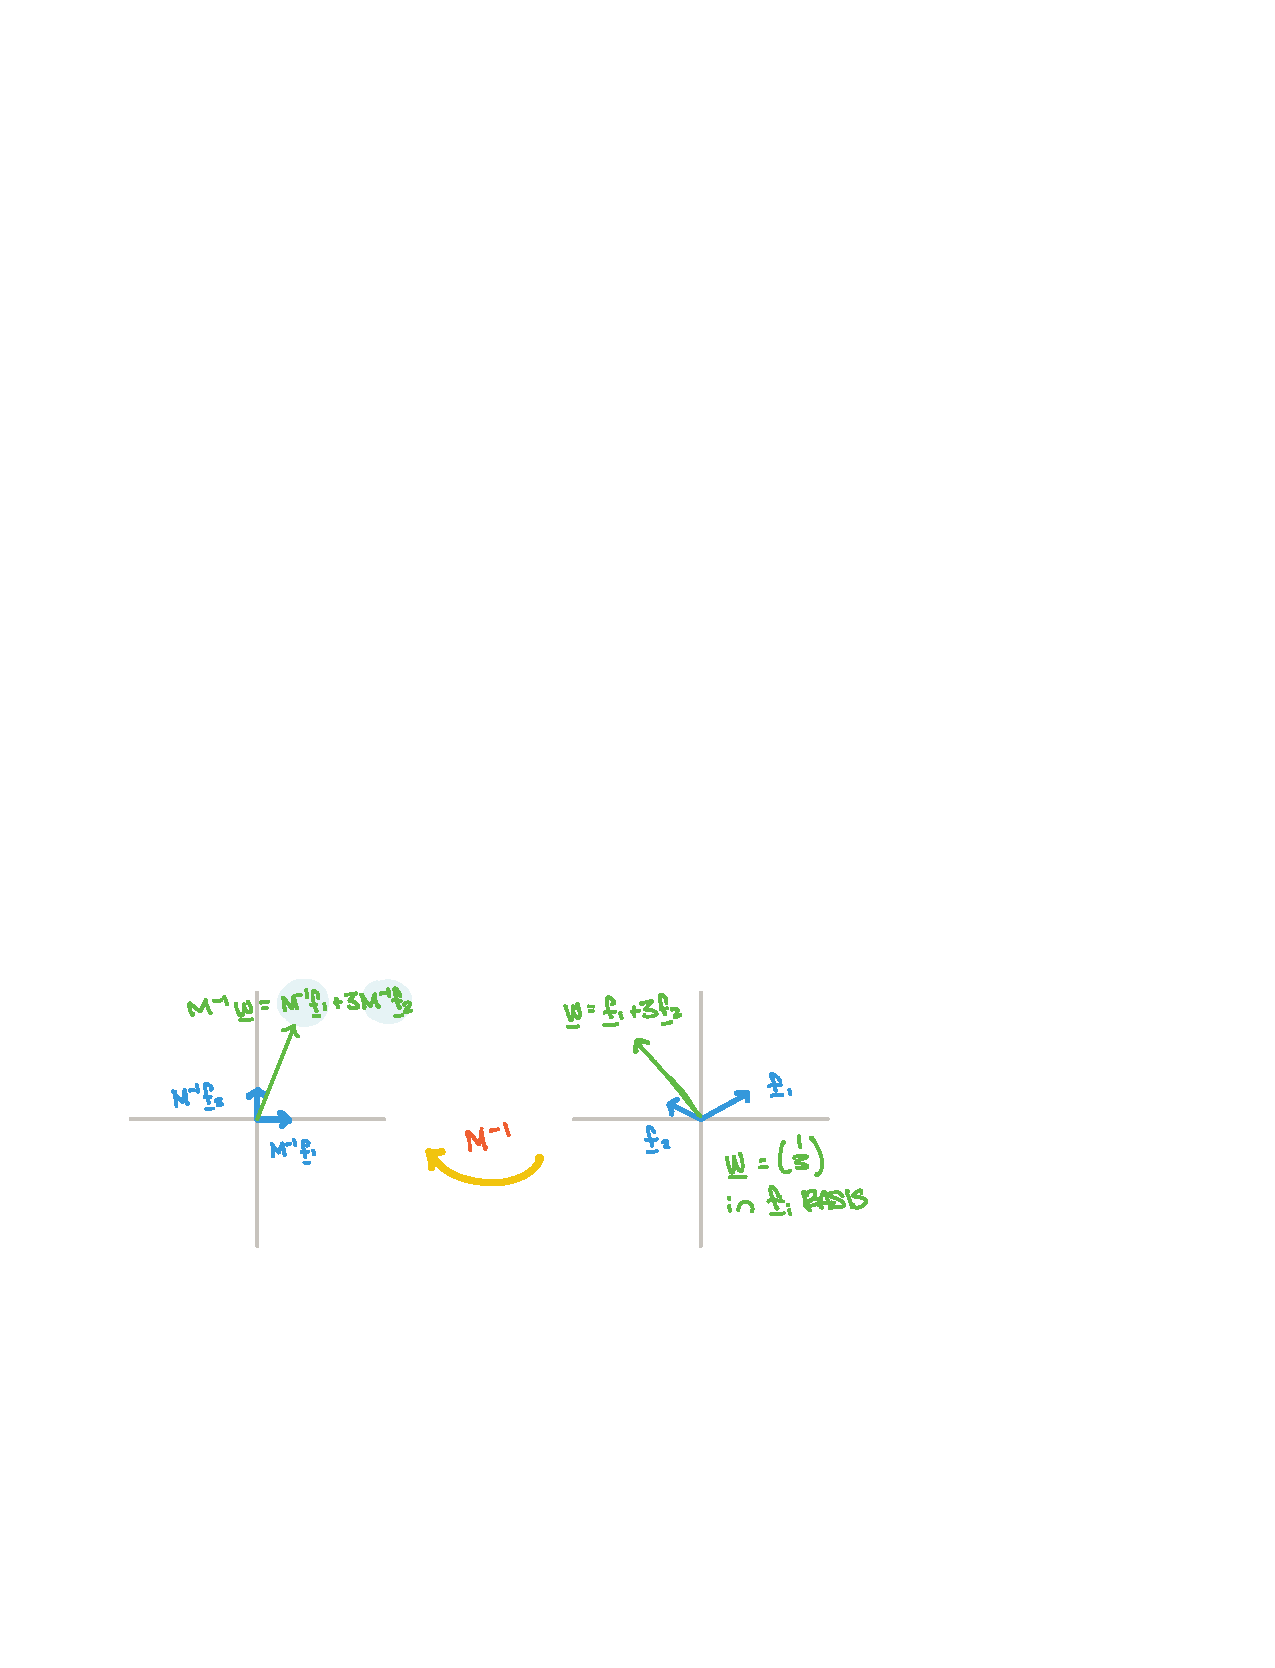
\includegraphics[width=.8\textwidth]{figures/maps_Minv.pdf}
    \caption{Let $M$ is a linear transformation from $\RR ^2 \to \RR ^2$, as we drew in Fig.~\ref{fig:map:M}. Now assume that you have a vector $\vec{w}$ that is the linear combination of some basis vectors $\vec{f}_i$, see the right-hand side of the sketch. If the $\vec{f}_i$ can be obtained as the transformation by $M$ of some other vectors---the basis vectors we called $\bas{e}_i$ in Fig.~\ref{fig:map:M}---then the inverse transformation $M\inv$ acts as a map ``back'' to the original basis. }
    \label{fig:map:M:inv}
\end{figure}

Given a basis, matrices are described by their components, $M\aij{i}{j}$. How do you find the components of the inverse matrix, $(M\inv)\aij{i}{j}$? The most straightforward way is the hard way. Let us consider the $2\times 2$ case. We know that the defining relationship is
\begin{align}
    M(M\inv)=(M\inv)M &= \one 
    &
    M\aij{i}{k}(M\inv)\aij{k}{j}
    =
    (M\inv)\aij{i}{k}M\aij{k}{j} 
    = \delta^i_j \ .
    \label{eq:inverse:matrix:definition}
\end{align}
On the right we have four equations for each combination of $i,j \in\{1,2\}$. We also have four unknown components, $(M\inv)\aij{i}{j}$. This is a system of linear equations that one can usually solve. Sometimes the system will not be solvable---in that case the matrix $M$ is not invertible.

\begin{exercise}
Convince yourself that \eqref{eq:inverse:matrix:definition} holds for \emph{any} vector space of any dimension, $N$. You end up with $N^2$ equations for $N^2$ unknown components $M\aij{i}{j}$. Does this change if all of the components are allowed to be complex numbers?
\end{exercise}


The product of two matrices $M$ and $N$ is a matrix, $MN$. The inverse of the product of matrices is the product of their inverses \emph{in the reverse order}
\begin{align}
    (MN)\inv = N\inv M\inv \ .
\end{align}
You can that this is because you have to undo the transformation that was last applied:
\begin{align}
    (MN)\inv MN = N\inv M\inv MN = N\inv \one  N = \one  \ .
\end{align}




\begin{example}
The inverse of a diagonal matrix is easy:
\begin{align}
    M &=
    \begin{pmatrix}
     3 & \pp  0 \\
     0 & -2
    \end{pmatrix}
    &
    M\inv &=
    \begin{pmatrix}
    \frac{1}{3} & \pp 0 \\
    0 & -\frac{1}{2}
    \end{pmatrix} \ .
\end{align}
We have used the fact that the product of diagonal matrices $\hat M$ and $\hat N$ is also a diagonal matrix whose elements are the products of the corresponding elements in $\hat M$ and $\hat N$.
\end{example}



\subsection{Basis of tensors}

 We may generalize to tensors by writing a generic tensor as:
 \begin{align}
    T =
     T\aij{i_1\cdots i_N}{j_1\cdots j_M}
     \ket{e_{i_1}}\cdots \ket{e_{i_N}}
     \bra{e^{j_1}}\cdots \bra{e^{j_M}} \ .
     \label{eq:tensor:T:with:basis}
 \end{align}
\begin{exercise}
Show how the index rules for tensors contraction onto other objects works using the bra-ket basis notation. Try making up some tensors, say $T^{ij} \ket{e_i}\ket{e_j}$ to see how it can contract onto other objects and use the defining relation \eqref{eq:basis:of:dual:vectors:bra:ket:form} to derive the usual index contractions. 
\end{exercise}

\begin{bigidea}[Tensors as linear functions]\label{idea:tensor:as:function}
Tensors are linear maps from some number of copies of $V$ and $V^*$ to numbers: a $(p,q)$ tensor is a map from $V^q \times (V^*)^p \to \#$. If we write such a tensor as $T\aij{i_1\cdots i_p}{j_1\cdots j_q}$, then these indices may contract with $p$ lower indices and $q$ upper indices to give a number. This is equivalently understood as a \emph{multi-linear} machine that takes in $q$ vectors and $p$ dual vectors to return a number. Here mutli-linear means that the machine is linear in each argument. 
\end{bigidea}

\begin{example}
Consider the $(2,1)$ tensor $T$ with components $T\aij{ij}{k}$. This is a map from $V\times V \times V^* \to \#$ because we may feed it a vector, $v^i$, and two row vectors, $w_j$ and $u_k$ to contract into a number:
\begin{align}
    T(\row{w},\row{u}, \vec{v})
    &=
    T\aij{ij}{k}v^k w_i u_j \ .
\end{align}
\end{example}

\begin{bigidea}[Tensors as linear maps]\label{idea:tensor:as:map}
Tensors are also linear maps between copies of vector spaces and dual vector spaces into other copies of vector spaces and dual vector spaces depending how its indices contract with other objects. A $(p,q)$ tensor $T$ may contract with an $(r,s)$ tensor $S$ such that:
\begin{itemize}
    \item Anywhere 
    \item from 0 to $\min(p,s)$ the upper indices of $T$ are contracted with the pairs of the lower indices of $S$.
    \item Anywhere from 0 to $\min(q,r)$ of the lower indices of $T$ are contracted with the upper indices of $S$.
\end{itemize}
Depending on these choices, the resulting object is a $(m,n)$ tensor where 
\begin{itemize}
    \item $m$ is from $[(p+q) - \min(p,s) - \min(q,r)]$, in the case of maximal contractions, to $(p+q)$, in the case of no contractions.
    \item $n$ is from $[(s+r) - \min(p,s) - \min(q,r)]$, in the case of maximal contractions, to $(s+r)$, in the case of no contractions.
\end{itemize}
\end{bigidea}

\begin{example}[Maps between product spaces]\label{eg:maps:between:product:spaces}
Example~\ref{eg:contraction:choices} and Exercise~\ref{eq:matrix:product:trace} demonstrate this for the case of two (1,1) tensors. 

Consider the case of a $(2,1)$ tensor $T\aij{ij}{k}$. Here are some possible contractions with different kinds of objects (we suppress the basis tensors and only write the components):
\begin{itemize}
    \item $T\aij{ij}{k}v^k$ is a (2,0) tensor $(T\vec{v})^{ij}$.
    \item $T\aij{ij}{k}w_i$ is a (1,1) tensor $(T\row{w})\aij{j}{k}$.
    \item $T\aij{ij}{k}M\aij{k}{\ell}$ is a (2,1) tensor $(TM)\aij{ij}{\ell}$
    \item $T\aij{ij}{k}M\aij{k}{j}$ is a (1,0) tensor $(TM)^i$.
    \item $T\aij{ij}{k}M\aij{\ell}{j}$ is a (2,1) tensor $(TM)\aij{ik}{\ell}$.
    \item $T\aij{ij}{k}T\aij{k\ell}{m}$ is a (3,1) tensor $(T^2)\aij{ij\ell}{m}$.
    \item $T\aij{ij}{k}T\aij{k\ell}{j}$ is a (2,0) tensor $(T^2)^{i\ell}$.
\end{itemize}
As practice, you are welcome to confirm all of this by including the bases `ket-bra' tensors. 
\end{example}

\begin{example}[Why ket-bras?]\label{eg:why:ketbra}
When writing a generic tensor in terms of its basis, say $T$ in \eqref{eq:tensor:T:with:basis}, we typically write these with kets first then bras.\sidenotemark This is a convention that makes it clear that none of the kets are acting on any of the bras.

What if you have a tensor where the order of the indices do not match the kets-first-then-bras convention? For example, a tensor:
\begin{align}
    Y = Y^{ij\phantom{k}\ell}_{\phantom{ij}k}
    \ket{e_i}\otimes\ket{e_j}\otimes\bra{e^k}\otimes\ket{e_\ell} \ ,
\end{align}
where we have used the \sout{X-men} tensor symbol $\otimes$ to make it clear that none of the bras or kets are acting on each other. This avoids any ambiguity, but it is cumbersome to write. (At least not without humming the theme song of the X-men animated series from the 1990s.)

In these cases, it is useful to simply \emph{define} a tensor where the order of indices is more convenient, but that otherwise contains the same information:
\begin{align}
    W = W\aij{ij\ell}{k} 
    \ket{e_i}\ket{e_j} \ket{e_k} \bra{e_\ell}
    \defeq 
    Y^{ij\phantom{k}\ell}_{\phantom{ij}k}
    \ket{e_i} \otimes \ket{e_j} \otimes \bra{e^k} \otimes \ket{e_\ell}
    \ .
\end{align}
This amounts to the component-wise identification
\begin{align}
    W\aij{ij\ell}{k} \equiv Y^{ij\phantom{k}\ell}_{\phantom{ij}k} \ .
\end{align}

\end{example}\sidenotetext{Notationally, kets and bras act on each other when the vertical lines match up, not when their angled parts point at each other.}

Observe that it can sometimes be ambiguous to know which bras and which kets are contracting with one another, so one may have to specify this explicitly. That is: if $T^{ij} \ket{e_i}\ket{e_j}$ is acting on $w_k\bra{e^k}$, which of $\ket{e_i}$ or $\ket{e_j}$ hits the $\bra{e^k}$? 

Practically when one has a tensor with several of the same type of basis bra or ket, one ends up symmetrizing or antisymmetrizing any contraction. This amounts to separating a tensor like $T^{ij} = T^{ij}_\textnormal{s} + T^{ij}_\textnormal{a}$ into a symmetric piece with $T_\textnormal{s}^{ij} = T_\textnormal{s}^{ji}$ and an antisymmetric piece with $T_\textnormal{a}^{ij}=-T_\textnormal{a}^{ji}$. Having done this, it does not matter \emph{which} of the `identical' indices you contract with because they are all treated on the same footing---at least up to a minus sign for the antisymmetric case. See Section~\ref{sec:permutation:symmerty} for the case of two lower indices. This sort of symmetrizing/antisymmetrizing game shows up in the representation theory of symmetries.
% Example: H2 dissociation

\begin{exercise}
Let $B_{ij}\bra{e^i}\bra{e^j}$ be a $(0,2)$ tensor. Separate it into a symmetric and an antisymmetric piece, $B = S+A$ where $S_{ij} = S_{ji}$ and $A_{ij} = - A_{ji}$. Assuming you know each component $B_{ij}$, write out each component $S_{ij}$ and $A_{ij}$.

Let $\vec{v} = v^i\ket{e_i}$ be a vector. Show that $B\ket{v}\ket{v} = S\ket{v}\ket{v}$. That is, show that
\begin{align}
    A\ket{v}\ket{v} = 0 \ .
\end{align}

Let $C^{ij}\ket{e_i}\ket{e_j}$ be an \emph{antisymmetric} $(2,0)$ tensor so that $C^{ij} = C^{ji}$. Show that $BC = AC$, or otherwise that
\begin{align}
    SC = 0 \ .
\end{align}

\textsc{Comment}: in each of these questions, there should be no ambiguity about which bras and which kets are contracted. If you worry that you have to make an arbitrary choice, check that the (anti-)symmetrization means that it does not actually matter up to a minus sign, provided that all objects that have multiple upper and/or multiple lower indices are symmetrized or anti-symmetrized.
\end{exercise}

 

\section{Transformation under symmetries}
\label{sec:transformation:under:symmetries}

Let us return to dancing around the really-big-idea of symmetries, even though we continue to be coy about actually defining these. We first introduced rotations in Section~
\ref{sec:Euclidean:three:space:rotations}, where we pontificated about the relation of rotations to the dot product because rotations leave vector lengths and angles between vectors unchanged. In Section~\ref{sec:isometry:first:pass:indices} we defined Rule~\ref{idea:transformation:of:upper:and:lower:indices} that told us how objects with indices transform. For example, in two-dimensional Euclidean space rotations that move the positive $x$-axis\sidenote{Here I should really say the $\bas{e}_1$ axis rather than the $x$-axis. This is because $x$ and $y$ are typically the coordinates what is called a `base space' or a base \emph{manifold}. In this section we refer to $x,y,$ and $z$ to appeal to our familiarity with three-space.} counter-clockwise (towards the positive $y$ axis) by and angle $\theta$ are $2\times 2$ matrices of the form
\begin{align}
    R(\theta)=
    \begin{pmatrix}
        \cos\theta & -\sin\theta \\
        \sin\theta & \pp \cos\theta
    \end{pmatrix} \ .
\end{align}
The following exercises introduce some of the machinery for rotations.
\begin{exercise}
If you have not done so yet, please confirm that $R(\theta)^\trans = R(\theta)\inv = R(-\theta)$.
\end{exercise}
\begin{example}
In three dimensions there are more kinds of rotations. One way to characterize this is to consider rotations about each coordinate axis. 
\begin{align}
    R_x(\theta) &= 
    \begin{pmatrix}
        1 & & \\
        &  \cos\theta & -\sin\theta \\
        & \sin\theta &  \pp\cos\theta 
    \end{pmatrix}
    \\
    R_y(\theta) &= 
    \begin{pmatrix}
        \pp \cos\theta & &\sin\theta \\
        & 1 & \\
        -\sin\theta& & \cos\theta
    \end{pmatrix}
    \\
    R_z(\theta) &= 
    \begin{pmatrix}
       \cos\theta & - \sin\theta & \\
        \sin\theta &\pp \cos\theta & \\
        & & 1
    \end{pmatrix}\ ,
    \label{eq:3D:rotation:matrices}
\end{align}
where all unlisted components are zero. Notice that these are all reshufflings of the rotations of the plane with the rotation axis held fixed---that should make sense. Also notice that the $R_y(\theta)$ rotation has the $-\sin\theta$ term in the lower-left while the other two rotations have it on the upper-right. This is to consistently apply the right-hand rule convention: a rotation about the $i^\textnormal{th}$ axis corresponds to gripping the axis with your right hand so that your thumb is pointing along the positive direction and identifying the direction that your fingers curl as the rotation direction. For each of these matrices, $R_i(\theta)^\trans = R_i(\theta)\inv = R_i(-\theta)$. 
\end{example}
\begin{exercise}
Taylor expand each of the three matrices in \eqref{eq:3D:rotation:matrices} and write them each in the form
\begin{align}
    R_i(\theta) = \one + i T_i \theta + \mathcal O(\theta^2) \ .
\end{align}
Here $i$ is the imaginary number, $i^2=1$, and the matrix $T_i$ is also pure imaginary.\footnote{This factor of $i$ is a convention in physics.} 

\textsc{Comment:}
The $T_i$ matrices are called \textbf{generators} each type of rotation. Physically, they represent the effect of an infinitesimal rotation about the respective axes. Infinitesimal rotations about other axes are given by \emph{linear combinations} of the $T_i$. In this way, the $T_i$ are a \emph{basis} for rotations.

Show that $T_xT_y - T_y T_x \propto T_z$ and determine the constant of proportionality. This relation is called an \emph{algebra} and denotes the mathematical structure of rotational symmetry.\footnote{This symmetry is called \SO{3}, the special orthogonal group of rank 3. Special means unit determinant, orthogonal means $R^\trans R = \one$.}
\end{exercise}

\begin{exercise}
The \emph{generator} of \SO{2}, rotations of the Euclidean plane, is
\begin{align}
    T = \begin{pmatrix}
        0 & i \\
        -i & 0
    \end{pmatrix} \ .
\end{align}
Show that $R(\theta) = \exp(iT\theta)$ where the matrix exponential is defined as its power series:
\begin{align}
    e^{M} = 1 + M + \frac{1}{2}M^2 + \cdots \ .
\end{align}
Use the power series expansion of the trigonometric functions. 
\end{exercise}

Assuming that we have a definition for which transformations are rotations,\sidenote{More generally, which transformations are \emph{isometries}. We finally present such a definition in Chapter~\ref{ch:metric:spaces}.} then we can examine how the basis vectors and row vector transform.

% Motivating the indices
% What is a symmetry



\subsection{Transformation of Vectors}\label{sec:active:passive}

To be somewhat philosophical: under an isometry like a rotation, there are two pictures to think about what happens to a vector:
\begin{itemize}
    \item \textbf{Active transformation}\index{active transformation}: your basis vectors stay put, but the vector is changing into a different vector, $\ket{v} \to \ket{v'}$. The components of $\ket{v'}$ are clearly different from the components of $\ket{v}$ because it the two are simply not the same vector.
    \item \textbf{Passive transformation}\index{passive transformation}: the vector \emph{does not change}, but the basis vectors change, $\ket{e_i} \to \ket{e'_i}$. This means that the components of $\ket{v}$ must \emph{also} change so that $v^i\ket{e_i} = v'^{i}\ket{e_i}$.
\end{itemize}
In an active transformation, the vector space and every vector in it change. In a passive transformation, the observer changes.\sidenote{There is something oddly Zen and philosophical about this.} For an isometry---a symmetry of the system---either perspective is valid. See Figures~\ref{fig:do:something} and \ref{fig:passive:rotation}.
% 

\begin{figure}[tb]
    \centering
    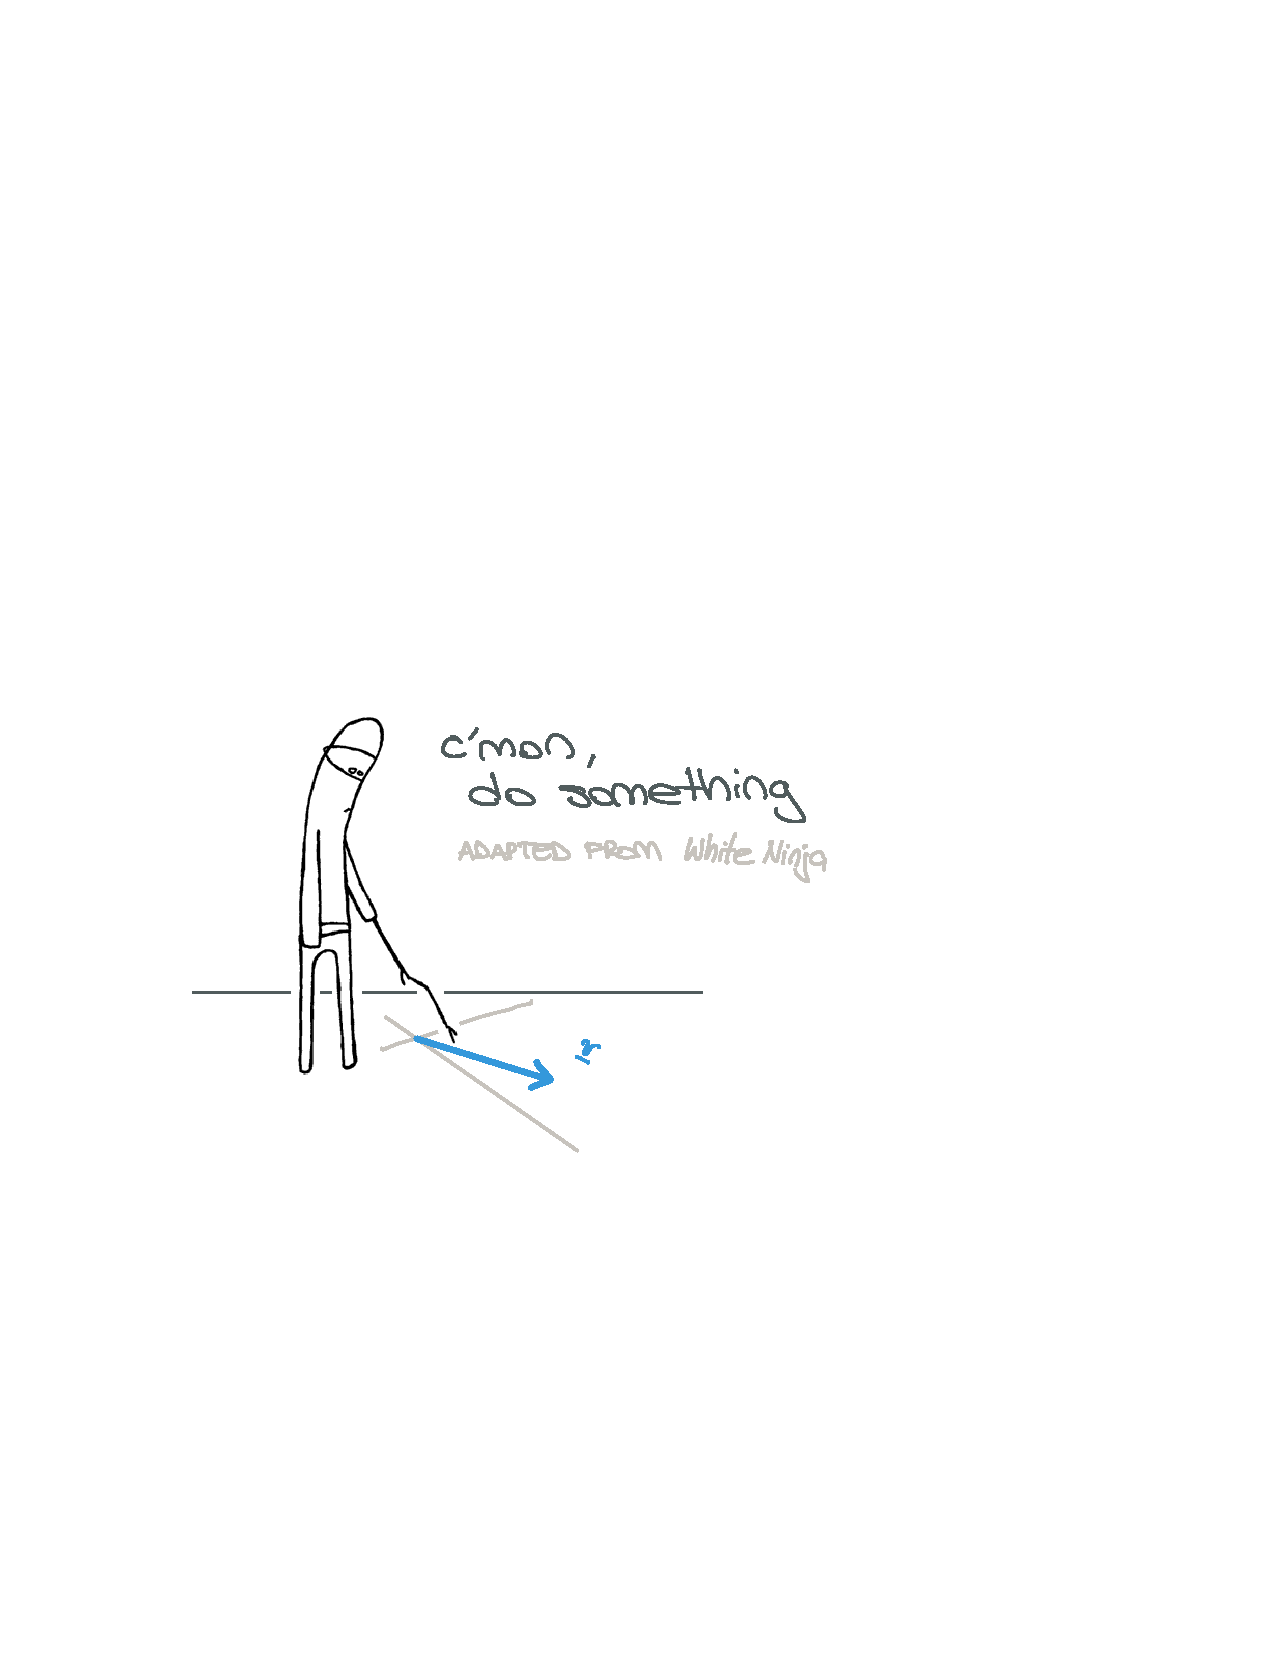
\includegraphics[width=.5\textwidth]{figures/passivetransform_dosomething.pdf}
    \caption{
        Nothing actually happens during a passive transformation. The basis vectors transform, but the components of the vector transform in such a way that $v'^i\bas{e}'_i = v^i\bas{e}_i$. Such a `transformation' may come off as uninspiring, but this is the basis of symmetries in physics. 
        From \url{https://knowyourmeme.com/memes/cmon-do-something}.
    }
    \label{fig:do:something}
\end{figure}

\begin{figure}[tb]
    \centering
    \includegraphics[width=.43\textwidth]{figures/rotate_1.pdf}
    \quad\quad
    \includegraphics[width=.43\textwidth]{figures/rotate_2.pdf}
    \caption{Example of a passive rotation. You are looking at a vector $\vec{v}$ through your phone. The image on your phone has a natural orientation for a basis $\bas{e}_i$ and the components of $\vec{v}$ in this basis are $v^i$. You could also rotate your phone, leaving the vector $\vec{v}$ untouched. The new basis vectors are $\bas{e}_i'$; they are different from $\bas{e}_i$ because your phone has changed orientation. With respect to the new basis, the same vector $\vec{v}$ now has components $v'^i$.}
    \label{fig:passive:rotation}
\end{figure}

Let $R(\theta)$ be the rotation about some axis by some angle $\theta$ that enacts a symmetry transformation. In the passive picture, vectors remain unchanged, but the basis vectors and the corresponding components do change:
\begin{align}
    \ket{v} = v^i \ket{e_i} =
    % v^i R\inv R \ket{e'_i}
    v^\ell R\aij{i}{\ell} (R\inv)\aij{\ell}{k}  \ket{e_k} \
    \defeq (v')^\ell \ket{e'_\ell}
    \ .
\end{align}
In the second equality we have simply inserted $\one = R R\inv$. On the right-hand side we \emph{define} the rotated components $v'$ and rotated basis vectors $\ket{e'}$ by absorbing the $R$ and $R\inv$ rotations:
\begin{align}
    (v')^i &\defeq R\aij{i}{\ell} v^\ell
    &
    \ket{e'_i} &\defeq  (R\inv)\aij{j}{i}\ket{e_j} \ .
    \label{eq:passive:transformation:of:vector:and:basis}
\end{align}
All we have done is collect into $v'^i$ all objects that contract with $v^ell$ and leave an object of a single upper index: that means that we absorb the $R\aij{i}{\ell}$. Similarly, we collect into $\ket{e'_i}$ all objects that contract with $\ket{e_j}$ and leave an object of a single lower index: that means we absorb the $(R\inv)\aij{j}{i}$. From this we have \emph{derived} the ``indexology rule'' \eqref{eq:components:of:vector:and:row:under:rotatino} which led us to the general tensor transformation in \bigidearef{}~\ref{idea:transformation:of:upper:and:lower:indices}.

Let me say that one more time: in \eqref{eq:passive:transformation:of:vector:and:basis} we are not \emph{applying} the rule that upper indices transform with $R$ and lower indices transform with $R\inv$. In fact, we are \emph{deriving it} from the condition that a passive [symmetry] transformation leaves the vector $\ket{v}$ unchanged while simply changing the basis and components of $\ket{v}$ while preserving $\ket{v}$.



To be clear, this choice of active versus passive pictures is only true for symmetries (isometries) where in some sense the system is not meaningfully changing. A general transformation that is \emph{not} an isometry should be thought of as an active transformation that change vectors.
\begin{example}
If we were to rotate the entire solar system, then it does not matter too much whether we think about this as some cosmic entity actually changing the configuration of every celestial object \emph{or} if we simply choose a rotated set of coordinates for the solar system. However, if we were to \emph{stretch} the solar system along one axis of the plane of the planets' rotation, then all of a sudden the planets would not be in stable orbits.\sidenotemark
\end{example}\sidenotetext{In this hypothetical: the coordinates do not change and Newton's laws do not change. Thus stretching the positions of each of the plants pulls them further away from the center of the sun without changing their angular momentum.}


\subsection{Transformation of Row Vectors}

The same argument holds for row vectors. For an isometry, one may take the passive transformation perspective in which row vectors do not transform, but we transform both the basis row vectors $\bra{e^i}$ and components of the row vector $w_i$ in such a way that $\bra{e^i}w_i \to \bra{{e'}^i}w'_i = \bra{w}$: 
\begin{align}
    w'_i &\defeq \tilde R\aij{\ell}{i} w_\ell
    &
    \bra{e'^i} &\defeq  (\tilde{R}\inv)\aij{i}{j}\bra{e^j} \ .
    \label{eq:passive:transformation:of:row:vector:and:basis}
\end{align}
In principle, this rotation $\tilde R$ is a different rotation from $R$. One may think think that $\tilde R$ has \emph{nothing to do} with the transformation of vectors, $v^i\ket{e_i} \to R\aij{i}{k}v^k(R\inv)\aij{\ell}{i}\ket{e_\ell}$. However, if $R$ and $\tilde R$ enact a symmetry of the system, then the transformations must preserve the defining relation of the dual vector basis \eqref{eq:basis:of:dual:vectors}, or the bra-ket form of that rule \eqref{eq:basis:of:dual:vectors:bra:ket:form}. This means we want to impose
\begin{align}
    \la e'^i \mid e'_j \ra \equiv \delta^i_j \ .
    \label{eq:basis:transform:under:rotation}
\end{align}
Inserting our expressions of the passively rotated basis elements relative to the original basis elements,\sidenote{We do this because we assume that the original basis elements satisfy $\la e^i \mid e_j \ra \equiv \delta^i_j$.}
\begin{align}
    \la e'^i \mid e'_j \ra &= 
    \la e^k \mid (\tilde{R}\inv)\aij{i}{k} (R\inv)\aij{\ell}{j} \mid e_\ell \ra
    =
    (\tilde{R}\inv)\aij{i}{k} (R\inv)\aij{\ell}{j} \la e^k \mid e_\ell \ra
    \\
    &=
    (\tilde{R}\inv)\aij{i}{k} (R\inv)\aij{\ell}{j} \delta^k_\ell
    =
    (\tilde{R}\inv)\aij{i}{k} (R\inv)\aij{k}{j} \ .
\end{align}
In order for this to equal $\delta^i_j$ we must have
\begin{align}
    (\tilde R)\inv R\inv = \one \ ,
\end{align}
or equivalently
\begin{align}
    \tilde R = R\inv \ ,
\end{align}
which is precisely what we motivate below \eqref{eq:R:Rtilde:transformation:from:indices:rotation}. 


\subsection{Transformation of Tensors}

Having established how $\ket{e_i}$ and $\bra{e^j}$ transform, the transformation of a general tensor---one composed of the tensor product of some number of bras and some number of kets---follows simply from the transformation of each bra and ket individually.

\begin{wide}
In this way, we may augment Rule~\ref{idea:transformation:of:upper:and:lower:indices} and \eqref{eq:transformation:of:upper:and:lower:indices} with the statement that from the passive transformation perspective, the basis tensors transform as
\begin{align}
    % T\aij{i_1\cdots i_N}{j_1\cdots j_M}
    % \to 
    % R\aij{i_1}{k_1}\cdots R\aij{i_N}{k_N}
    % (R\inv)\aij{\ell_1}{j_1}\cdots (R\inv)\aij{\ell_N}{j_N}
    % T\aij{k_1\cdots k_N}{\ell_1\cdots \ell_M} \ .
    % \label{eq:transformation:of:upper:and:lower:indices}
    \ket{e_{i_1}} \cdots \ket{e_{i_N}}
    \bra{e^{j_1}} \cdots \bra{e^{j_M}}
    \to 
    (R\inv)\aij{k_1}{i_1}\cdots (R\inv)\aij{k_N}{i_N}
    R\aij{j_1}{\ell_1}\cdots R\aij{j_N}{\ell_M}
    \ket{e_{k_1}} \cdots \ket{k_{i_N}}
    \bra{e^{\ell_1}} \cdots \bra{e^{\ell_M}} \ .
\end{align}
For completeness, here is how the components transform:
\begin{align}
    T\aij{i_1\cdots i_N}{j_1\cdots j_M}
    \to 
    R\aij{i_1}{k_1}\cdots R\aij{i_N}{k_N}
    (R\inv)\aij{\ell_1}{j_1}\cdots (R\inv)\aij{\ell_M}{j_M}
    T\aij{k_1\cdots k_N}{\ell_1\cdots \ell_M} \ .
    \tag{\ref{eq:transformation:of:upper:and:lower:indices}}
\end{align}
\end{wide}

Let us observe that the rule we proposed in Rule~\ref{idea:transformation:of:upper:and:lower:indices} is simply a \emph{byproduct} of our definition of how the basis bras and kets transform. In fact, it is the product of the definition of how \emph{either} the basis bras or the basis kets transform, since the transformation law of the other type of object necessarily follows from \eqref{eq:basis:transform:under:rotation}.

\begin{example}[Moment of inertia]
The moment of inertia tensor has two lower indices.\footnote{This may depend on conventions. It is certainly true that the moment of inertia tensor has two indices that are both the same height.} Explain why it transforms differently from a matrix, which has one upper and one lower index.
\end{example}

\subsection{(Non-)Transformation of Numbers}

Numbers---perhaps you want to call them scalars---do not transform. They have no free indices to transform. Some numbers have contracted indices. Consider a bra $\bra{w}$ acting on $M$, which in turn acts on a $\ket{v}$,\sidenote{You can alternatively say that $M$ is acted on by both $\bra{w}$ and $\ket{v}$, or many other combinations.}
\begin{align}
    \la w \mid M \mid v \ra 
    &= 
    w_i \bra{e^i} \; M\aij{j}{k}\ket{e_j}\!\bra{e^k}
    \; v^\ell \ket{e_\ell} 
    \\&=
    w_i M\aij{i}{k}v^k 
    \ ,
\end{align}
where we have used the defining relation $\la e^i\mid \ra e_j = \delta^i_j$. These combinations are invariant and no longer transform. That's why we may use the $\delta$ function to collapse sums. We are left with a transformation law
\begin{align}
    w_i M\aij{i}{k}v^k 
    \to 
    w_\ell(R\inv)\aij{\ell}{i} \, R\aij{i}{m}
    M\aij{m}{n} (R\inv)\aij{n}{k} \, R\aij{k}{p} v^p \ .
\end{align}
We find two instances of the contraction $(R\inv)\aij{a}{b}R\aij{b}{c} \equiv \delta^a_c$, which shows that the right-hand side is identical to the left-hand side. In this way an object whose indices are fully contracted does not transform. 

\begin{exercise}
Analogously, an object with some contracted indices and some uncontracted indices \emph{does} transform, but only according to the uncontracted indices. If $T_{ik}$ is a (0,2) tensor, show that $T_{ik}v^k$ transforms like a row vector by transforming each pf $T_{ik}$ and $v^k$ independently and showing that one factor of $R$ and one factor of $R\inv$ cancel each other out.
\end{exercise}




\section{Dropping the Basis Tensors... Again}

In Section~\ref{sec:component:notation} we presented tensors the way that most physicists use tensors: objects with indices. In the rest of this chapter, we built up the machinery of basis linear maps that form the underlying structure of what tensors are. This helps us understand how the components of a tensor transform when we change basis. By virtue of the defining relation between basis bras and kets, \eqref{eq:defining:bra:ket:relatin}, you may have found that once we all agree upon a basis, then \emph{all of those basis tensors are kind of redundant}!

In other words, when there is no ambiguity about basis, I could have just written $v^i$ and you would \emph{know} that the only possible thing that I could mean is $v^i\ket{e_i}$. Similarly, the matrix $M\aij{i}{j}$ could \emph{only} possibly mean $M\aij{i}{j}\ket{e_i}\!\bra{e^j}$. This is because we know that all of these objects are intrinsically index-free---the indices all contract with the appropriate basis objects. This then leads us to the idea that maybe we could just \emph{drop} the basis tensors and just write everything as objects with indices.

Everything we have said in this chapter is still true and still \emph{under the hood}, so to speak. But you will find that physicists find it most convenient to work in the shorthand of just writing the \emph{components} of tensors with the implicit understanding of there being a contraction with basis tensors.\footnote{Roger Penrose proposes formalizing this shorthand in what is called \emph{abstract index notation}. A good online discussion is this one: \url{https://math.stackexchange.com/questions/455478/}} 



\begin{subappendices}


\section{Permutation Symmetry}\label{sec:permutation:symmerty}

Our favorite objects thus far---vectors, dual vectors, and matrices---have been refreshingly \emph{unambiguous} in the following sense: If you are looking to contract indices, you know \emph{exactly} which indices can contract. An ambiguity arises when we have a tensor that has multiple upper or lower indices. Consider the following example of a (0,2) tensor $A$ acting on a vector $\ket{v}$:
\begin{align}
    B_{ij}\bra{e^i}\bra{e^j} \; v^k \ket{e_k} \ .
\end{align}
The following two statements are equivalent:
\begin{itemize}
    \item There is an ambiguity about which of the two bras, $\bra{e^i}$ or $\bra{e^j}$, contracts with the basis ket $\ket{e_k}$. 
    \item In the shorthand where we do not write the basis tensors, there is an ambiguity about which of the lower $i$ or $j$ indices of the matrix $B$ contracts with the upper index of the $\vec{v}$.
\end{itemize}
\begin{exercise}
Show that both of these statements are equivalent by using \eqref{eq:defining:bra:ket:relatin}. 
\end{exercise}
One way to break the degeneracy is to explicitly specify \emph{which} contraction we really want---this is in the spirit of Example~\ref{eg:contraction:choices}. There is a trick that we often employ: take symmetric and antisymmetric combinations of the indices.

For our purposes, let us stick to the case of tensors with two lower indices like $B$ above. The trick is to separate the components of $B$ into a symmetric and an antisymmetric part:
\begin{align}
    B_{ij} &= S_{ij}+A_{ij}
\end{align}
where these pieces are 
\begin{align}
    S_{ij} &= \frac{1}{2} \left(B_{ij} + B_{ji}\right)
    \\
    A_{ij} &= \frac{1}{2} \left(B_{ij} - B_{ji}\right) \ .
\end{align}
\begin{exercise}
Decompose the (0,2) tensor $B_{ij}$ below\footnote{For ease of notation we have written the components of $B_{ij}$ as a square array of numbers. This does not mean that $B$ is a matrix---at least not in the sense of being a (1,1) tensor. This is simply for notation. When writing out the components of any two-index tensor in ``matrix multiplication'' notation, there is no way to distinguish between (2,0), (1,1), and (0,2) tensors.} into its symmetric and antisymmetric parts:
\begin{align}
    \begin{pmatrix}
        B_{11} & B_{12}\\
        B_{21} & B_{22}
    \end{pmatrix}
    =
    \begin{pmatrix}
        1 & 2\\
        0 & 3
    \end{pmatrix} \ .
\end{align}
\end{exercise}


\begin{exercise}
A basis of symmetric and antisymmetric (0,2)-tensors are:
\begin{align}
    \la{e^{(i}}|\la{e^{j)}}|
    \defeq&
    \frac{1}{2}\left( 
        \bra{e^i}\bra{e^j} + \bra{e^i}\bra{e^j}
    \right)
    \\
    \la{e^{[i}}|\la{e^{j]}}|
    \defeq&
    \frac{1}{2}\left( 
        \ket{e^i}\bra{e^j} - \ket{e^i}\bra{e^j}
    \right) \ .
\end{align}
The factor of $1/2$ is conventional. The subtle curved-versus-square bracket notation is also a standard convention. How would you perform the projection that takes $(0,2)$ tensors into their symmetric parts? What about their antisymmetric parts?

Show that if $S_{ij} = S_{ji}$ is symmetric, then 
\begin{align}
     S_{ij}\la{e^{[i}}|\la{e^{j]}}| = 0 \ .
 \end{align}
\end{exercise}


The symmetric tensor is especially nice:
\begin{quote}
When contracting a symmetric tensor $S_{ij}$ with a vector, it does not matter which index one contracts with. 
\end{quote}
Let us see this in action\sidenote{We simply contract components---if you want, you can write this in full bra-ket notation with the basis tensors written out. It is a good exercise if you are not used to it.}:
\begin{align}
    S_{ij}v^j = S_{ji}v^j \ .
\end{align}
We use the symmetry of $S$ to show that we could have equivalently contracted with the first index or the second. Note that the free index needs to remain the same in order for the equality to make sense: we are looking at the $i^\text{th}$ component of $S\ket{v}$.

We can see this in action for a contraction with two vectors as well:
\begin{align}
    S_{ij}v^iw^j = S_{ji}v^i w^j = S_{ij} v^j w^i \ .
    \label{eq:symmetric:with:two:vectors}
\end{align}
In the last equality we simply relabel the contracted (`dummy') indices.

The antisymmetric tensor is also nice, though slightly less so. Here we have
\begin{align}
    A_{ij}v^j = - A_{ji}v^j \ .
\end{align}
The effect of whether we contract with the first or the last index is an overall minus sign. For a double contraction:
\begin{align}
    A_{ij}v^iw^j = -A_{ji}v^i w^j = -A_{ij} w^i v^j \ .
\end{align}
In the last line we have deliberately swapped the order of $w^i v^j$---which commute---to make this look suggestively similar to the cross product. \flip{To fill in: connection of Levi-Civita symbol to cross product in three dimensions.}





\begin{exercise}
Convince yourself that all of our discussion here holds for tensors with two upper indices. Further, convince yourself that the discussion holds if $B$ happened to also have an upper index: $B\aij{i}{jk}$. Finally, convince yourself that if $B$ had two upper and two lower indices, $B\aij{ij}{k\ell}$, one could separately symmetrize and antisymmetrize each index.
\end{exercise}



\section{\texorpdfstring{The Kronecker $\delta$}{The Kronecker Delta}}\label{sec:kronecker}

The Kronecker $\delta$ is defined to be
\begin{align}
    \delta^i_j = 
    \begin{cases}
        1 &\text{ if }i=j \\
        0 &\text{ otherwise}
    \end{cases} . 
\end{align}
A useful way to think of this is that $\delta^i_j$ are the components of the identity matrix:
\begin{align}
    \one = \delta^i_j \ket{e_i}\bra{e^j} \ .
\end{align}
Unlike typical matrix components, we write the indices vertically aligned because there is no ambiguity about the ordering: any component for which the ordering matters is already zero.\sidenote{This makes the $\delta^i_j$ stick out a bit as if it were reminding us that \emph{hey, I'm just the identity}. Most likely we just use this convention because it is easier to type up in \LaTeX.}

Think of $\delta^i_j$ as a tool to collapse sums.
\begin{example}
Consider the contraction $\delta^i_j v^j$. Expanding this gives:
\begin{align}
    \delta^i_j v^j = 
    \delta^i_1 v^1
    +
    \delta^i_2 v^2
    +
    \delta^i_3 v^3
    + 
    \cdots
\end{align}
For any specific $i$, only one of the terms is non-zero. For example,
\begin{align}
    \delta^{i=2}_j v^j = 
    \cancel{\delta^2_1} v^1
    +
    \delta^2_2 v^2
    +
    \cancel{\delta^i_3} v^3
    + 
    \cdots
    = 
    v^2 \ .
\end{align}
\end{example}


\begin{example}\label{eq:double:sum:delta}
Consider the double sum $w_i \delta^i_j v^j$ \ .
\begin{align}
    w_i \delta^i_j v^j = &
    \pp w_1 \delta^1_1 v^1 + w_1 \cancel{\delta^1_2} v^2 + \cdots \\
    &+ w_2 \cancel{\delta^2_1} v^1 + w_2 \delta^2_2 v^2 + \cdots \\
    =& w_1v^1 + w_2 v^2 + \cdots = w_iv^i \ .
\end{align}
\end{example}

The example above gives us a rule to use the Kronecker $\delta$ to collapse sums:
\begin{newrule}
Whenever the $j$ index in $\delta^i_j$ contracts with the upper index of a tensor, you can simply replace that upper index with the $i$ from the $\delta^i_j$. Similarly, whenever the $i$ index in $\delta^i_j$ contracts with the lower index of a tensor, you can simply replace that lower index with the $j$ from the $\delta^i_j$.
\end{newrule}

\begin{example}
Consider the contraction between two general tensors:
\begin{align}
    S\aij{i_1\cdots i_N i}{j_1\cdots j_M} T\aij{k_1\cdots k_P}{\ell_1\cdots \ell_Q \ell}
    \delta^\ell_i &= 
    S\aij{i_1\cdots i_N i}{j_1\cdots j_M} T\aij{k_1\cdots k_P}{\ell_1\cdots \ell_Q i}
    \\
    &=
    S\aij{i_1\cdots i_N \ell}{j_1\cdots j_M} T\aij{k_1\cdots k_P}{\ell_1\cdots \ell_Q \ell}\ ,
\end{align}
where in the second line we simply show that it does not matter whether you replace the upper or lower index.
\end{example}


\begin{example}
Sometimes it is helpful to see something written in gory detail. Let us write out even more terms in Example~\ref{eq:double:sum:delta}:
\begin{align}
    w_i \delta^i_j v^j = 
    &
    \pp w_1 \delta^1_1 v^1 
    + w_1 \cancel{\delta^1_2} v^2 
    + w_1 \cancel{\delta^1_3} v^3 
    + w_1 \cancel{\delta^1_4} v^4 
    + \cdots 
    \\
    & 
    + w_2 \cancel{\delta^2_1} v^1
    + w_2 {\delta^2_2} v^2 
    + w_2 \cancel{\delta^2_3} v^3 
    + w_2 \cancel{\delta^2_4} v^4 
    + \cdots 
    \\    & 
    + w_3 \cancel{\delta^3_1} v^1
    + w_3 \cancel{\delta^3_2} v^2 
    + w_3 {\delta^3_3} v^3 
    + w_3 \cancel{\delta^3_4} v^4 
    + \cdots 
    \\    & 
    + w_4 \cancel{\delta^4_1} v^1
    + w_4 \cancel{\delta^4_2} v^2 
    + w_4 \cancel{\delta^4_3} v^3 
    + w_4 {\delta^4_4} v^4 
    + \cdots 
    \\
    = &
    \pp w_1 \delta^1_1 v^1 
    \phantom{+ w_1 \cancel{\delta^1_2} v^2 }
    \phantom{+ w_1 \cancel{\delta^1_3} v^3 }
    \phantom{+ w_1 \cancel{\delta^1_4} v^4 }
    \phantom{+ \cdots }
    \\
    & 
    \phantom{+ w_2 \cancel{\delta^2_1} v^1}
    + w_2 {\delta^2_2} v^2 
    \phantom{+ w_2 \cancel{\delta^2_3} v^3 }
    \phantom{+ w_2 \cancel{\delta^2_4} v^4 }
    \phantom{+ \cdots }
    \\    & 
    \phantom{+ w_3 \cancel{\delta^3_1} v^1}
    \phantom{+ w_3 \cancel{\delta^3_2} v^2 }
    + w_3 {\delta^3_3} v^3 
    \phantom{+ w_3 \cancel{\delta^3_4} v^4 }
    \phantom{+ \cdots }
    \\    & 
    \phantom{+ w_4 \cancel{\delta^4_1} v^1}
    \phantom{+ w_4 \cancel{\delta^4_2} v^2 }
    \phantom{+ w_4 \cancel{\delta^4_3} v^3 }
    + w_4 {\delta^4_4} v^4 
    + \cdots 
    % & w_1v^1 + w_2 v^2 + \cdots = w_iv^i 
    \\
    =& w_1v^1\phantom{\delta^i_j} + w_2 v^2\phantom{\delta^i_j} + w_3 v^3\phantom{\delta^i_j} + w_4 v^4\phantom{\delta^i_j} \cdots 
    \\=& w_iv^i 
    \ .
\end{align}
The key here is to first understand why several terms are zero, then to learn the `rule of thumb' that the $\delta^i_j$ reduces a double sum into a single sum. Any time you have a repeated index where one of the repeated indices is on a Kronecker-$\delta$, you can simply remove the Kronecker $\delta$ and replace that index with the \emph{other} index on $\delta$. In the example above, we saw that there was a repeated $j$ index in $w_i \delta^i_j v^j$. We found that we can simply remove the $\delta$ and replace the $v^j$ with $v^i$ because $i$ is the `other' index on $\delta^i_j$.
\end{example}

\section{Canceling factors in a tensor equation}

% \begin{wide}
Sometimes you will find equations of the following form:
\begin{align}
    w_i M\aij{i}{j}v^j = w_i A\aij{i}{j}v^j \ .
    \label{eq:canceling:factors:wMv}
\end{align}
If we were to expand this, the equation reads:
\begin{align}
    &w_1 M\aij{1}{1}v^1 + w_1 M\aij{1}{2}v^2
    + w_2 M\aij{2}{1}v^1 + w_2 M\aij{2}{2}v^2
    \\
    =&
    w_1 A\aij{1}{1}v^1 + w_1 A\aij{1}{2}v^2
    + w_2 A\aij{2}{1}v^1 + w_2 A\aij{2}{2}v^2 \ ,
    \label{eq:canceling:factors:wMv:long}
\end{align}
where we take the two-dimensional case for brevity. 
% \end{wide}

Based on this equation, can you infer anything about how the matrices $M$ and $A$ relate to one another? Not by itself since the equation seems to depend on the values of $w_i$ and $v^j$. 

However, if we further said that \eqref{eq:canceling:factors:wMv} is true \emph{for any vector $\vec{v}$ and any dual vector $\row{w}$}, then we can deduce that 
\begin{align}
    M\aij{i}{j} = A\aij{i}{j} \ ,
\end{align}
the two matrices are equivalent. This is clear in the expanded form of the equation. If you set $w_1 = v^2 = 1$ while $w_2 = v^1 = 0$, then \eqref{eq:canceling:factors:wMv:long} reduces to $M\aij{1}{2} = A\aij{1}{2}$. You can do this for any choices of the $\row{w}$ and $\vec{v}$ components. This leads us to want to take \eqref{eq:canceling:factors:wMv} and \emph{cancel} the common factors on both sides:
\begin{align}
    \cancel{w_i} M\aij{i}{j} \cancel{v^j} = \cancel{w_i} A\aij{i}{j} \cancel{v^j} \ ,
    \label{eq:canceling:factors:wMv:cancel}
\end{align}
which indeed gives us the equality $M=A$. Note that we can \emph{only} do this when we mandate that \eqref{eq:canceling:factors:wMv} is true for \emph{any} $\row{w}$ and $\vec{v}$.
\begin{example}
Suppose
\begin{align}
    M &= 
    \begin{pmatrix}
        1 & 3 \\
        7 & 3
    \end{pmatrix}
    &
    A&=
    \begin{pmatrix}
        1 & 3\\
        2 & 3
    \end{pmatrix} \ .
\end{align}
If we choose
\begin{align}
    \row{w} &=
    \begin{pmatrix}
        1 & 0
    \end{pmatrix}
    &
    \vec{v} &=
    \begin{pmatrix}
        1 \\ 0
    \end{pmatrix} \ ,
\end{align}
then \eqref{eq:canceling:factors:wMv} is true. However, if we instead choose 
\begin{align}
    \row{w} &=
    \begin{pmatrix}
        0 & 1
    \end{pmatrix}
    &
    \vec{v} &=
    \begin{pmatrix}
        1 \\ 0
    \end{pmatrix} \ ,
\end{align}
then \eqref{eq:canceling:factors:wMv} is not true. The equality of each component of $M$ and $A$ requires that \eqref{eq:canceling:factors:wMv} is true for \emph{any} $\row{w}$ and $\vec{v}$. 
\end{example}


The `cancel on both sides' step in \eqref{eq:canceling:factors:wMv:cancel} is curious in that we are canceling a objects that have indices that are summed over with the rest of an expression. You went from an equation between sums of many terms to an equation that related specific terms in that sum. Alternatively, you went from an equation between two numbers to an equation between the components of two matrices. These components, of course, represent specific terms in \eqref{eq:canceling:factors:wMv:long} that that may be singled out on each side of the equation by judicious choice of $\row{w}$ and $\vec{v}$. 

A word of caution is in order. When doing this trick, you should start by writing out the dummy indices\sidenote{Dummy indices are indices that are contracted over: they appear twice in an expression, once as an upper index and once as a lower index.} in such a way that the factors that you are canceling have \emph{exactly} the same index names. Thus it is true that we may rewrite the right-hand side of \eqref{eq:canceling:factors:wMv} as 
\begin{align}
    w_i A\aij{i}{j}v^j = w_a A\aij{a}{b}v^b \ ,
\end{align}
and it is even true that 
\begin{align}
    w_i M\aij{i}{j}v^j = w_a A\aij{a}{b}v^b \ .
\end{align}
However, we cannot then write that
\begin{align}
    M\aij{i}{j} = A\aij{a}{b} \ ,
\end{align}
because the indices between the left-hand and right-hand sides of this equation make no sense: when $i=1$ and $j=2$, what do $a$ and $b$ correspond to? It may be obvious in this simple example because there is a unique upper and lower index, but this can become rather subtle.


\end{subappendices}

\chapter{Interlude on Bundles}\label{ch:bundles}


Over the last few chapters, we have taken a very concrete picture of vectors and have made it successively more abstract. At this point, physics students are well in their right to ask: where are there vector spaces in physics?\sidenote{This interlude is ``for culture'' and is outside the main narrative of the course.}

\section{Tangent Planes}


Consider the sphere---perhaps this is the surface of the Earth. We are little specks on the surface of the sphere. To be fancy, we call this sphere a \textbf{manifold}\index{manifold}.\sidenote{You can think of this as a possibly curvy space of positions.} To each us, the world appears to be flat.\sidenote{We say that \emph{locally} our space appears to be flat.} We can make a chart of our local \emph{neighborhood} and draw a \emph{map} on a piece of paper where we describe the apparently-flat space around us, see \bigidearef{}~\ref{idea:2d:chart}. We can imagine that this map is a plane that is tangent to the surface of the earth.
% 
\begin{marginfigure}%[th]
    \includegraphics[width=\textwidth]{figures/TangentBundle.pdf}
    \captionsetup{font={scriptsize,sf}}
    \caption{Two tangent planes, $\textnormal{T}_{p_{1,2}M}$ over a manifold $M$. A curve $\gamma(t)$ through the manifold has velocity vectors $\dot{\gamma}(t)$ that live in the tangent planes at each point $\gamma(t)=p_i$.}
    \label{fig:tangent:bundle:sphere}
\end{marginfigure}
% 

If we were somewhere else on the sphere, perhaps in the southern hemisphere, then we would again observe a locally flat space that we could imagine as a tangent plane. Figure~\ref{fig:tangent:bundle:sphere} draws two such tangent planes, perhaps as seen by an observer from far away, like the International Space Station. In the figure, the two tangent planes are called $\textnormal{T}_{p_1}M$ and $\textnormal{T}_{p_2}M$. The key observation in this example is that the tangent planes at different points $p_1$ and $p_2$ are similar, but they have \emph{different orientations}. Viewed from the International Space Station, it is clear that the vectors in $\textnormal{T}_{p_1}M$ live in a totally different vector space than those in $\textnormal{T}_{p_2}M$. From the perspective far away from earth, the vectors on these tangent planes actually have \emph{three} components. Accounting for the third dimension, the \emph{span} of vectors in $\textnormal{T}_{p_1}M$ is different from the span of vectors in $\textnormal{T}_{p_2}M$.


In this figure we have also drawn a path, $\gamma(t)$. You can imagine this as the trajectory of someone journeying from the south pole to the north pole.\sidenote{Like those old \emph{Indiana Jones} cuts between scenes that shows the airplane on the map.} In this notation, $\gamma(t)$ specifies the longitude and latitude of the traveler as a function of time, $t$. The time derivative $\dot\gamma(t)=\D{\gamma}/\D{t}$ is the \emph{velocity vector} at the point $p=\gamma(t)$. This velocity vector lives in the tangent plane at $p$. As the traveler moves along $\gamma(t)$, its tangent plane rotates.\sidenote{Apparently the technical word for this is \emph{osculates}. Feel free to use that word in your everyday life, but I doubt it will impress anyone.} 

This poses a mathematical problem: what does it mean for the traveler to move with \emph{constant velocity} if the velocity vectors live in different vector spaces. These vector spaces are not even oriented in the same way in three-dimensional space! The connection between the linear vector spaces $\textnormal{T}_pM$ and the underlying curvy space $M$ is called \textbf{differential geometry}\index{differential geometry} and is the mathematical bedrock of general relativity. One does not need to be so highfalutin to see this structure---it is the underlying framework of phase space in particle mechanics. 



\section{No position vectors}\label{sec:no:position:vectors}

Vectors in physics live in structures like these tangent planes. With the appropriate amount of abstraction, \emph{every}\sidenote{I think this is true for every vector. I may be wrong, but I do not know of any good counterexamples.} vector in physics can be viewed as a ``velocity'' of some path along some manifold. These manifolds do not necessarily represent space or spacetime; they may be rather abstract.\sidenote{For example, the space of $2\times 2$ matrices} The collection of all of the tangent spaces to a manifold is called the \textbf{tangent bundle}\index{tangent bundle}. It represent the space of all possible velocity vectors at all points on the manifold.

The key question in differential geometry is how to connect these tangent spaces together. For the tangent bundle of the sphere, the \emph{geometry} tells us how to connect the nearby tangent planes so that ideas like ``constant velocity'' are well defined. The mathematical object that connects these nearby tangent spaces is something that is called a \textbf{connection}\index{connection}---yeah, it is not the most inspired name.\sidenote{For those who have read ahead: observe that this does not necessarily require a metric, only a connection. However, if you have a metric, there is typically an `obvious' connection that is compatible with the metric. This is like saying: if you have a Mac, you probably also have an iPhone.}

% \begin{marginfigure}%[th]
%     \includegraphics[width=\textwidth]{figures/base_space_tangent_space.pdf}
%     \captionsetup{font={scriptsize,sf}}
%     \caption{The base space is ``coordinate space.'' These are positions. Positions are not vectors and the base space is not a vector space. Positions depend on the coordinate system. At each position $(x,y)$, there is a vector space called the tangent space at $(x,y)$. This \emph{is} a vector space and the vectors can be thought of as possible velocities of a particle at $(x,y)$. In the picture on the right hand side we have `peeled' the base space away from the tangent space to make it clear that they are different, even though they both look like sheets of paper. There is no assumed curvature in the base space. There is a different tangent space for each position. The combination of the infinite number of tangent spaces over the base space is known as a tangent space bundle.}
%     \label{fig:tangent:space:polar}
% \end{marginfigure}

\begin{figure}[tb]
    \centering
    \includegraphics[width=.7\textwidth]{figures/base_space_tangent_space.pdf}
    \caption{The base space is ``coordinate space.'' These are positions. Positions are not vectors and the base space is not a vector space. Positions depend on the coordinate system. At each position $(x,y)$, there is a vector space called the tangent space at $(x,y)$. This \emph{is} a vector space and the vectors can be thought of as possible velocities of a particle at $(x,y)$. In the picture on the right hand side we have `peeled' the base space away from the tangent space to make it clear that they are different, even though they both look like sheets of paper. There is no assumed curvature in the base space. There is a different tangent space for each position. The combination of the infinite number of tangent spaces over the base space is known as a tangent space bundle.}
    \label{fig:tangent:space:polar}
\end{figure}

The tangent bundle picture of vectors also explains the following maxim that I have repeated over and over:
\begin{quote}
\emph{There is no such thing as a position vector.}
\end{quote}
Vectors live in a tangent space $\textnormal{T}_pM$. On a tangent space there is a natural meaning of the zero vector: it is the case of zero velocity. However, \emph{positions} live on the manifold, $M$. There is \emph{no} natural meaning of a `zero' position: that is simply an arbitrary choice of the origin of coordinates. Because the origin has no significance, there is also no natural meaning for taking a linear combination of positions.\sidenote{On the other hand, \emph{differences} of positions \emph{can} have physical meanings since they do not depend on an arbitrary origin.}

\begin{example}
In a vector space, the zero vector is special because it is the additive identity. Any vector plus the zero vector is well defined: it returns the vector itself,
\begin{align}
    \vec{v} + \vec{0} = \vec{v} \ .
\end{align}
If I define a coordinate system for space, the zero point of that coordinate system means nothing. There is no meaningful sense in which you can \emph{add} that position to another position, let alone for it to be understood to be the additive identity. 

However, differences of positions are meaningful vectors. The zero vector is when two points are coincident. Adding the zero vector does not change the separation between two points. 
\end{example}


\section{Taylor Expansion, yet again}

Curved manifolds are, unsurprisingly, much more difficult than flat ones. One way of seeing the preponderance of vector spaces in physics is that these vectors are the leading terms in the evolution of a system whose trajectory on a manifold is $\gamma(t)$. That we write the velocity vector as $\dot\gamma(t)$ shows a significant relationship between derivatives and vector spaces. 

Suppose you have some function $f(p)$ that takes points on the manifold $p\in M$ and returns a number. For example, $f(p)$ may be the temperature at the point $p$ on the Earth. Given a trajectory $\gamma(t)$ on the Earth, one may ask that at a given time $t$ and point $p=\gamma(t)$, what is the instantaneous rate of change of the temperature? Let us write $\gamma^i(t)$ to mean the $i^\textnormal{th}$ coordinate of $\gamma(t)$.\sidenote{Note that $\gamma^i(t)$ is not the component of a vector. It is a component of a position, and positions are not vectors.}
% 
With respect to the ambient three dimensional space, this rate of change is
\begin{align}
    \dot f(\gamma(t)) = \frac{\D{f(\gamma(t))}}{\D{t}} = 
    \frac{\partial f}{\partial \gamma^i}
    \frac{\D{\gamma^i(t)}}{\D{t}}
    % \frac{\partial f(t)}{\partial x^i}  \frac{\partial x^i}{\partial t} \bas{e}_i \ ,
\end{align}
Here we recognize that $v^i= \D{\gamma^i(t)}/\D{t}$ \emph{is} the component of a vector. This is because \emph{differences} of positions are vectors, even if positions themselves are not. Thus we may write
\begin{align}
    \dot f(\gamma(t)) %= \frac{\D{f(\gamma(t))}}{\D{t}} = 
    \frac{\D{\gamma^i(t)}}{\D{t}}
    \frac{\partial}{\partial \gamma^i}
    f(\gamma(t))
    =
    v^i
    \frac{\partial}{\partial \gamma^i}
    f(\gamma(t)) \ .
    % \frac{\partial f(t)}{\partial x^i}  \frac{\partial x^i}{\partial t} \bas{e}_i \ ,
\end{align}
We recognize that\sidenote{I use the notation $\partial_x = \frac{\partial}{\partial x}$.} $v^i \partial_{\gamma^i}$ looks like a velocity vector with a basis given by the partial derivatives. Indeed, we often write that this allows us to treat the partial derivatives with respect to the manifold $M$ are a \emph{basis} for the tangent space.\sidenote{In this case the sphere is embedded in the three dimensional space, so there are possible three basis vectors. However, each tangent space is two dimensional. This is consistent because $v^i= \D{\gamma^i(t)}/\D{t} = 0$ in the direction that is perpendicular to the surface. Thus one linear combination of partial derivatives always has a zero coefficient.} This idea of a vector as a linear combination of partial derivatives is quite helpful, albeit completely unusual the first time you see it. One can imagine that this sort if picture shows up all the time when dealing with flows.



\section{Microphysics lives in the tangent plane}

We present this picture as if you already know what the trajectory $\gamma(t)$ is. In physics, we often try to solve the opposite problem.  If you know the properties of a trajectory at some point $p=\gamma(0)$, can you \emph{integrate} the equations of motion to determine the trajectory at future times?\sidenote{The question of integrability of a vector field over a manifold is an open one in many important physical scenarios. Look up the phrase `integrable system.'}

A bit more philosophically: the laws of physics are defined microscopically. They relate the dynamics of the system at one point to the dynamics at nearby points. This is why our theories are all written with differential operators. Taking the picture that the tangent planes are approximations for moving along the manifold, everything that we call \emph{physics}\sidenote{Notably, equations of motion and the underlying structures from which they are derived.} is defined on how these tangent planes relate to each other. In this way, we can measure things like arclength on a trajectory by using the \emph{metric} (see Chapter~\ref{ch:metric:spaces}) and summing together the infinitesimal lengths of tangent vectors along the trajectory. The components of the metric are a \emph{field}\index{field} defined on the manifold, $g_{ij}(x)$. This means that the `rulers' we use to measure distance are warped if space is curved.\sidenote{The requirement that the connection between tangent planes may be metric compatible is one about the $x$-dependence of the components of the metric.} In general relativity, gravity is encoded in the metric. 

\section{Diffeomorphisms}

Often the tensors on the tangent bundle are defined with respect to the coordinates of the base space, $x$. As you saw in the previous sections, these can show up as partial derivatives with respect to these coordinates, which are a natural\sidenote{Natural, if somewhat unexpected.} basis for the tangent planes. The way we choose to place coordinates on a manifold, however, is not a property of the manifold: it is simply a choice that we make. Thus all these bundles must not depend on whether we choose one reasonable set of coordinates versus another. This is called \emph{diffeomorphism invariance}. When we change coordinates on $M$, say from $x\to y,$ the quantities on the tangent planes also change coordinates. Because those quantities are written with respect to partial derivatives, the transformations look like\sidenote{Note that an upper index in the denominator contracts like a lower index. It is one of the convenient quirks of the summation convention. Convince yourself that this makes sense.}
\begin{align}
    \frac{\partial}{\partial x^i} \to 
    \frac{\partial y^j}{\partial x^i} 
    \frac{\partial}{\partial y^j}  \ .
\end{align}
Thus in relativity you will often see change of coordinates written as ${\partial y^j}/{\partial x^i}$. On a given tangent plane, these play the role of generalized rotation matrices.


\begin{bigidea}
Through this part of the course, the rules for how a tensor transforms in Section~\ref{sec:transformation:under:symmetries} are true for \emph{any} transformation, including diffeomorphisms if one is on a bundle. In that section and in most of this course, we focus only on the case when these transformations are rotations (or their generalizations, isometries). The reason for this is that in Chapter~\ref{ch:metric:spaces} we introduce the inner product, which defines a special class of transformations---rotations (isometries)---which are the main focus of our course. However, an object with indices is a tensor if it transforms tensorially under \emph{any} transformation, including diffeomorphisms. 
\end{bigidea}
The above \bigidearef{} comes up again in Section~\ref{sec:Levi:Civita:Tensor:vs:Symbol} when we look at an object called the Levi-Civita tensor.



\section{Bundles of Fun}

The rich structure of vector spaces and dual vector spaces become richer on a bundle. Just as there is a tangent bundle $\textnormal{T}_pM$, there is also a co-tangent bundle $\textnormal{T}^*_pM$ where dual vectors live. There are other types of fields that live on the manifold and tell us about how to move between the spaces that live `over' a point $p$. If you are mathematically inclined, a good way to start thinking about bundles is to think about the M\"obius strip as the prototype of a bundle with non-trivial \emph{global} properties, see e.g.\ Collinucci and Wijns\autocite{Collinucci:2006hx}.

For more introductory references on how this structure appears in ordinary mechanics, I refer to two neat graduate-level textbooks in Fig.~\ref{fig:figure:mathematical:physics:books}. If you want to deeply appreciate the differences between the Lagrangian and Hamiltonian formulation of mechanics, you may enjoy these books. For example, momenta are part of the cotangent bundle while velocities are part of the tangent bundle. 
\begin{marginfigure}%[th]
    \includegraphics[width=.6\textwidth]{figures/Arnoldbook.jpg}\\
    \includegraphics[width=.6\textwidth]{figures/MCP_Thorne.jpg}
    \captionsetup{font={scriptsize,sf}}
    \caption{Two excellent references to go over some physics that you know (mechanics) in the language of differential geometry.}
    \label{fig:figure:mathematical:physics:books}
\end{marginfigure}

The fundamental forces in subatomic physics are part of a structure called a \textbf{gauge theory }\index{gauge theory} which is mathematically a bundle over spacetime. Unlike tangent or co-tangent bundles, the vector space living `on top' of each point $p$ needn't strictly be a tangent space. These vector spaces are called fibers. In electromagnetism, the fiber is the choice of gauge.\sidenote{Recall from electrodynamics that the vector and scalar potentials can be shifted by the derivative of a function of spacetime. This is called gauge symmetry.} This gauge is a redundancy in how we describe a system. The redundancy is necessary to maintain manifest spacetime symmetries in the theory. The \emph{connection} on such a structure is called the gauge potential---this is precisely the vector and scalar potentials. In the quantum version of electrodynamics, this gauge potential is the quantum field associated with the photon. Analogously, there is a fiber bundle picture for fundamental forces---such a picture exists for gravity as well, though I have never had the occasion to make use of it. 


\chapter{Metric Spaces}\label{ch:metric:spaces}

Prior to this chapter we have developed the theory of vector spaces, dual vector spaces, and the tensor products of these spaces. We defined the relation between these spaces with respect to linear maps. This, in turn, gave further insight on how the basis imposed on a vector space is translated to its dual space. We presented the idea that a tensor could be used to convert one type of object into another. 

In this chapter we see what happens when we \emph{define} an \emph{additional} machine on this structure. This machine is a special tensor called the \textbf{metric}, also known as the \textbf{dot product}, \textbf{inner product}. By defining this structure, we \emph{upgrade} or vector space into what is called a \textbf{metric space}\index{metric space}---a vector space equipped with a metric. This upgrade unlocks our ability to define key ingredients for geometry: length and angle. In turn, this allows us to describe special relativity a language naturally attuned to it.\sidenote{Having come this far, you may see that we have worked hard to build a mathematical machinery. The example of special relativity is our first payoff: it is not that we want to build unnecessarily sophisticated mathematics, it is that building the mathematical machine lets us write actual physical phenomena in a \emph{succinct} language that highlights physical principles. That is: I would rather understand relativity as a unification of space and time under a metric rather than as a cobbled together list of otherwise unrelated rules.}

\section{Metric and Inner Product}

The metric and inner product are so closely related that they are \emph{essentially} the same idea. The \textbf{metric} is a special (0,2)-tensor that we write as
\begin{align}
    g_{ij}\bra{e^i}\bra{e^j} \ .
\end{align}
Often physicists just write the \emph{components} of the metric, $g_{ij}$, and assume that you all agree on the basis.\sidenote{There's more to this. Usually the metric defines for us what a `nice' basis is. When physicists simply write $g_{ij}$ without telling you the basis, it is usually because the \emph{only} nice bases are the components of the metric are the same.} By definition, the components of the metric are symmetric:
\begin{align}
    g_{ij} = g_{ji} \ .
\end{align}

Why should we consider symmetric metrics? Part of the answer is the observation in Section \ref{sec:permutation:symmerty} that symmetric (0,2) tensors remove the ambiguity of having to define which of the metric's lower indices contracts when offered another tensor's upper index. Another post-facto justification is that the way we use the metric to define lengths and angles is naturally symmetric.

\begin{example}
The \textbf{Euclidean metric}\index{Euclidean metric} is
\begin{align}
    g_{ij} = 
    \begin{cases}
        1 &\text{ if } i = j \\
        0 &\text{ otherwise} \ .
    \end{cases}
    \label{eq:metric:euclidean}
\end{align}
When written as an array of numbers, it is simply the identity matrix.\footnote{Though clearly as an object with two lower indices it is a (0,2) tensor, \emph{not} a matrix---which is what we call (1,1) tensors.}
You may wonder if this is the same as the Kronecker $\delta$ from Section~\ref{eq:kronecker:delta}. It may have the same components when written as an array, but it is \emph{not} the same. The Kronecker $\delta$ is a (1,1) tensor, whereas a metric is a (0,2) tensor. They may have the same numerical values of their components, but they are completely different objects.\footnote{Pick your favorite convergent evolution example to use as an analogy. Sharks and dolphins look remarkably similar, even though one is a fish and the other is a mammal.} 

You could write $g_{ij} = \delta^i_j$, but this is a very strange-looking equation since the index heights do not match. That equation is true component wise---meaning ``plug in any values for $i$ and $j$''---but it is not true if you think this is a tensorial relation:
\begin{align}
    g_{ij}\bra{e^i}\bra{e^j} \neq \delta^i_j \ket{e_i}\bra{e_j} \ .
\end{align}
\end{example}

\begin{example}\label{eg:Minkowski:metric}
The metric for Minkowski space (special relativity) is
\begin{align}
    g_{\mu\nu} = \eta_{\mu\nu}
    =
    \begin{cases}
    \pp 1 & \text{if } \mu=\nu = 0\\
    -1 & \text{if } \mu=\nu > 0\\
    \pp 0 & \text{otherwise}
    \end{cases} \ .
    \label{eq:Minkowski:metric}
\end{align}
We introduce some conventional notation. First, the special relativity metric is called $\eta_{\mu\nu}$ whereas the general relativity (with gravity) metric is called $g_{\mu\nu}$. Second, we distinguish between time and space by indexing time as $\mu=0$. In order to remind us that the indices start with zero, we use lowercase letters from the middle of the Greek alphabet ($\mu, \nu$) instead of $i,j$.

About a quarter of physicists use this form of the metric. This tribe includes nearly all particle physicists. Another quarter or so use the convention where $\eta_{\mu\nu}^\text{grav.} = -\eta_{\mu\nu}$. This group includes gravitational physicists and formal theorists (what we used to call string theorists). The other half could not care less about the metric of spacetime. 
\end{example}

From the metric one can define the \textbf{inner product}\index{inner product}, which in Euclidean space is what we call a \textbf{dot product}\index{inner product}. This is a function that uses the metric to take in two vectors to return a number:\sidenote{You would be correct in wondering how this is at all different from the metric itself. From the linear map perspective, any (0,2) tensor is \emph{defined} to be a function that takes two vectors and returns a number, $V\times V \to \#$. In this sense, the inner product is \emph{literally} the same as the metric. However, conventionally colleagues say \emph{metric} to mean the components and \emph{inner product} to mean the function. By now we all agree that these really encode same thing.}
\begin{align}
    \la \vec{v},\vec{w} \ra = g(\vec{v},\vec{w})
    = g_{ij} v^i w^j \ .
\end{align}
Because of the symmetry of $g_{ij}$, we have
\sidenote{By the way, please appreciate that we now freely moving between our different conventions for referring to tensors---$v^i$, $\vec{v}$, $\ket{v}$---based on whichever is \emph{most convenient} for the case at hand. This avoids cumbersome notation, like writing an inner product using ket notation, for example: $\la \ket{v}, \ket{w} \ra$. }
\begin{align}
    \la \vec{v}, \vec{w} \ra = \la \vec{w}, \vec{v} \ra \ .
\end{align}



\begin{exercise}
Show that the components the metric are easily (perhaps \emph{tautologically}\footnote{This is a mathematicians way of saying `obvious.' In fact, it is more than that. It is something that Anthony Zee calls ``more obvious than obvious'' (I think I picked this up from his quantum field theory book). What this means is that the fact is so `by definition' self-apparent that any attempt to explain it will only obfuscate the matter.}) expressed as inner products of the basis vectors:
\begin{align}
    g_{ij} = \la \bas{e_i}, \bas{e_j}\ra \ .
\end{align}
\end{exercise}

There is one more practical requirement for a metric: the metric is invertible. Another way of saying this is that it is \emph{non-degenerate}. 

\section{A tool to define length}
\label{sec:machine:to:make:row:vectors}

The \textbf{length}\index{length} of a vector $\vec{v}$ is defined by
\begin{align}
 |\vec{v}|^2  
 = \la \vec{v},\vec{v} \ra 
 = g_{ij}v^iv^j
 \ .
 \label{eq:lenght:in:terms:of:metric}
\end{align}

\begin{exercise}
Observe that if the metric had any antisymmetric part, then it would cancel in its contribution to the length. 
\end{exercise}

\begin{example}
For the case of the Euclidean metric \eqref{eq:metric:euclidean}, the length is exactly what one expects from plane geometry: a vector is some arrow starting at the origin whose length is determined by an application of the Pythagorean theorem. One obvious observation is that any Euclidean vector with non-zero components has non-zero length.
\end{example}

\begin{example}
For the case of the Minkowski metric \eqref{eq:Minkowski:metric} in (1+1)-dimensions\footnote{It is conventional to write the dimension of Minkowski space as a sum of the time and space dimensions.} the length of a vector is:
\begin{align}
    |\vec{v}|^2 = (v^0)^2 - (v^1)^2 \ .
    \label{eq:minkowski:length:2d}
\end{align}
Unlike Euclidean space, you can have a Minkowski space vector, say 
\begin{align}
    v^\mu = 
    \begin{pmatrix}
        7\\
        7
    \end{pmatrix} \ ,
\end{align}
that has obviously non-zero components but has \emph{zero length}. We call these \textbf{null vectors}\index{null vector}. In fact, any such vector in (1+1)-dimensional Minkowski space with $|v^0| = |v^1|$ is a null vector.
\end{example}

\begin{exercise}
Argue that in any metric space, the length of the vector is a square root of some expression that is quadratic in the components of the vector. In other words, there can be no metric spaces where something weird happens like
\begin{align}
    |\vec{v}| = \sqrt[3]{(v^1)^2 + v^1v^2 - (v^2)^2}
\end{align}
or perhaps
\begin{align}
    |\vec{v}| = (v^1)^3 - (v^2)^2 \ .
\end{align}
You can argue this purely based on the mathematical definition of a metric space. As a physicist, these definitions also make no sense the moment you think about units.
\end{exercise}

Because the length is just a number, we can rescale any vector by its length to get a \textbf{unit vector}\index{unit vector}, a vector with unit length:
\begin{align}
    \hat{\vec{v}} \defeq \frac{\vec{v}}{|\vec{v}|} \ .
\end{align}
We say that vectors with unit length are \textbf{normalized}\index{normalized}. 


\section{A tool to define angles}

Given two vectors $\vec{v}$ and $\vec{w}$, the \textbf{angle}\index{angle} between these vectors is defined by
\begin{align}
    \cos\theta = \frac{\la \vec{v}, \vec{w} \ra}{|\vec{v}| |\vec{w}|}
    =
    \la \hat{\vec{v}}, \hat{\vec{w}} \ra \ .
    \label{eq:cos:theta:angle:defined:metric}
\end{align}
Because the metric and inner product are symmetric, the cosine of the angle between two vectors does not depend on the order of the vectors.\sidenote{There is a notion of the angle from $\vec{v}$ to $\vec{w}$ being negative that of the angle from $\vec{w}$ to $\vec{v}$. This is called orientation. However, because cosine is an even function, $\cos\theta = \cos(-\theta)$, and so the definition for the cosine of the angle in terms of the inner product is robust. One just has to remember that inverting the cosine has multiple solutions.}

\begin{exercise}
Show that the angle between two vectors is independent of the length of the vector. 
\end{exercise}

\begin{exercise}
Show that in (1+1)-dimensional Minkowski space two vectors may each be \emph{null} (zero length), $\la \vec{v},\vec{v}\ra =0$, but may have non-zero angle with one another. Give an explicit example.  \textsc{Hint}: the condition for a vector to be null has two solutions. Check the inner product of the two.
\end{exercise}


\section{A tool to lower indices}
\label{{sec:machine:to:make:row:vectors}}

The following observation is, by far, the most common way to think about the metric:
\begin{quote}
The metric is a machine that takes an upper index and returns a lower index.
\end{quote}
That this is true is obvious: any (0,2) tensor is a linear map from vectors to dual vectors. We know this from the discussion in Example~\ref{eg:maps:between:product:spaces}. Here's how it works in full tensorial glory:
\begin{align}
    g_{ij}\bra{e^i}\bra{e^j} \; v^k \ket{e_k}
    &= 
    g_{ij}v^k \delta^j_k \; \bra{e^i}
    =
    g_{ij}v^j\; \bra{e^i}
    % \defeq v_i \bra{e^i} 
    \ .
    \label{eq:metric:lowering:full:tensor}
\end{align}
\begin{exercise}
Use the fact that the metric is symmetric to show that one obtains the same result if we contract the $\bra{e^i}$ with the $\ket{e_k}$ rather than the $\bra{e^j}$ with the $\ket{e_k}$ in \eqref{eq:metric:lowering:full:tensor}. That is:
\begin{align}
    g_{ij}\bra{e^i}\bra{e^j} \; v^k \ket{e_k}
    = 
    g_{ij}\bra{e^j} \; v^k \la {e^i}\mid {e_k}\ra \
    =
    g_{ji}v^i \bra{e^j}
    \ .
\end{align}
\end{exercise}

What is significant here is that when we define the metric space, we require that everyone agrees on the definition of the metric. That means that given a vector $\ket{v} = v^i\ket{e_i}$ in a metric space with a metric $g_{ij}\bra{e^i}\bra{e^j}$,\sidenote{Usually we would just say ``given a vector $v^i$ and a metric $g_{ij}$'' and leave the tensor basis implicit.} we can make the following \emph{definition}:
\begin{align}
    v_i \defeq g_{ij}v^j \ .
\end{align}
Let us spell out exactly what is going on:
\begin{enumerate}
    \item Until this point, there was \emph{no object} whose component carries a single lower index. We only assumed that you have a vector (one upper index) and a metric (two lower indices). 
    \item Now we have defined a new object $v_j$ who shares the same variable name as the vector $v^i$, except with a lower index.
    \item This lower-object version of $v^i$ is defined to be the contraction of $v^i$ with the metric. It is completely expected that this contraction gives an object with a lower index, but usually we would call it $(gv)_i = g_{ij}v^j$.
    \item Since there is no other object that (a) has the variable name $v$ \emph{and} (b) carries a single lower index, we choose to \emph{define} $v_i = g_{ij}v^j$. 
    \item Because we are in a metric space, we assume everyone knows what the metric is. That means there is no ambiguity about how to form $v_i$ from $v^j$: it is \emph{understood} that we use the metric. So as a shorthand, we stop writing the metric explicitly.
\end{enumerate}

We generalize this to lower any index on a tensor with an upper index:
\begin{newrule}[Lowering indices with the metric]
Suppose you have a tensor whose components include some upper index, say $T\aij{ijk}{\ell}$. If you see a tensor with the \emph{same variable name} but with that index lowered, then it is \emph{understood} that this means
\begin{align}
    T\aij{ij}{k\ell} \defeq g_{km}T\aij{ijm}{\ell} \ .
\end{align}
\end{newrule}
Now that we have a rule to lower indices, please be careful that you must \emph{preserve the order of the indices}! 
\begin{example}
If you have a tensor with components $T\aij{ijk}{\ell}$, then $T\aij{ij}{k\ell}$ is different from $T^{i\phantom{j}k}_{\phantom{i}j\phantom{k}\ell}$. Explicitly:
\begin{align}
    T\aij{ij}{k\ell} = g_{km}T\aij{ijm}{\ell}
    \neq
    T^{i\phantom{j}k}_{\phantom{i}j\phantom{k}\ell}
    = g_{nj}T\aij{ink}{\ell} \ .
\end{align}
\end{example}
\begin{example}
We can lower multiple indices. Suppose you have a tensor whose components include some upper index, say $T\aij{ijk}{\ell}$. Then we have an implicit definition for the tensor with all of its indices lower:
\begin{align}
    T_{ijk\ell} = g_{im}g_{jn}g_{kp}T\aij{mnp}{\ell} \ .
\end{align}
\end{example}

\section{Is this a transpose?}

At this point, it is natural to draw on your familiarity with matrix algebra and to think that the metric seems to ``tip over'' a column vector and turn it into a row vector. You may ask, as the popular meme in Figure~\ref{fig:is:this:a:transpose}, whether we are defining a transpose. We are \emph{not}.
\begin{marginfigure}%[th]
    \includegraphics[width=\textwidth]{figures/IsThisTranspose.jpg}
    \captionsetup{font={scriptsize,sf}}
    \caption{The metric is \emph{not} a transpose. ``Is This a Pigeon'' meme via \url{https://imgflip.com/i/8nc9fd}.}
    \label{fig:is:this:a:transpose}
\end{marginfigure}

\begin{example}[Tipping over a column vector?]
In \emph{Euclidean space}, lowering an index with the metric is apparently equivalent to ``tipping over'' the column vector. As an explicit example, consider a vector
\begin{align}
    \vec{v}=
    \begin{pmatrix}
        v^1\\v^2\\v^3
    \end{pmatrix}
    =
    \begin{pmatrix}
        1\\2\\3
    \end{pmatrix} \ .
\end{align}
By acting on this vector with the metric, we produce a row vector with components $v_i = g_{ij}v^j$. Using the trivial Euclidean metric \eqref{eq:metric:euclidean}, this says that the component with the upper index is the same as the component with the lower index:
\begin{align}
    \row{v} = 
    \begin{pmatrix}
        v_1 & v_2 & v_3
    \end{pmatrix}
    =
    \begin{pmatrix}
        1 & 2 & 3
    \end{pmatrix} \ .
\end{align}
So indeed, it looks like we just knocked the column vector over and it is now lying down flat---but the components are all the same. 

In any other space, the numerical values of the row vector are rather different. Consider the Minkowski metric \eqref{eq:Minkowski:metric}. Once again, we start with a column vector with the same components---though in line with the Minkowski convention in Example~\ref{eg:Minkowski:metric} we index starting from 0:
\begin{align}
    \vec{v}=
    \begin{pmatrix}
        v^0\\v^1\\v^1
    \end{pmatrix}
    =
    \begin{pmatrix}
        1\\2\\3
    \end{pmatrix} 
    \ .
\end{align}
As before, the components of the row vector are $v_\mu = g_{\mu\nu}v^\nu$, where the content of this equation is \emph{identical} to $v_i = g_{ij}v^j$ except that we use the physics convention of writing spacetime indices with Greek indices. Then our row vector has \emph{different} components:
\begin{align}
    \row{v} = 
    \begin{pmatrix}
        v_0 & v_1 & v_1
    \end{pmatrix}
    =
    \begin{pmatrix}
        1 & -2 & -3
    \end{pmatrix} \ .
\end{align}
\end{example}

\begin{exercise}
Consider a 2-dimensional metric space whose metric contains---rather annoyingly---off-diagonal elements:
\begin{align}
    g_{ij} = \begin{pmatrix}
        g_{11} & g_{12} \\
        g_{21} & g_{22}
    \end{pmatrix}
    =
    \begin{pmatrix}
        1 & \varepsilon \\
        \varepsilon & 1
    \end{pmatrix} \ ,
\end{align}
for some constant $\varepsilon$. If you have a vector $\vec{v} = v^i \bas{e}_i$, what are the components of the corresponding dual vector $\row{v} = v_i \rbas{e}^i$? Make sure that this matches the Euclidean case when $\varepsilon\to 0$.
\end{exercise}

So let us emphasize: using the metric to lower an index is \emph{not} a transpose. There is a proper definition of transpose for matrices, but there is no such thing as the `transpose of a vector.' One feature that is useful from that otherwise incorrect notion is that the tensor with a metric-lowered index physically encodes the same content as the original tensor. In this way, it is the `same' tensor.

\begin{bigidea}[Is it a `different' tensor?]
Conceptually, \emph{in a metric space}, you should think of $\ket{v} = v^k \ket{e_k}$ and $\bra{k} = v_k \bra{e^k}$ as the `same' essential object, but with different components reflecting whether the object is being used as a vector or a dual vector. This is usually the case in physical applications. For example, in relativity the four-momentum---a vector containing the energy and the three spatial momenta---is a vector. The dual vector may have different components---the metric introduces minus signs on the spatial components---but we understand it to encode the same ``energy and the three spatial momenta'' as the upper-indexed object.
\end{bigidea}



\begin{example}
The fact that the Euclidean metric is so boring is part of the reason why we often take it for granted. Many first-time learners of linear algebra (done properly) are confused why row vectors and column vectors are treated differently. In these lectures we emphasized that when you only have a vector space and not a metric space, you cannot convert between vectors and row vectors. The vector spaces that we grow up with---Euclidean three-space---implicitly have a metric. After all, you grew up `knowing' how to take the length of a vector or the angle between vectors.\footnote{Of course, many of us also grow up with the completely wrong idea that positions are vectors.} 

The challenge here is to realize that when we were young, we had been \emph{assuming} the existence of a metric without explaining that it is an additional structure that we can choose---as in the case of Minkowski space. I grew up in a household where every meal came with rice. It never occurred to me that there might be other starches that could form the base of a meal. The first time I went to a grade school friend's house for dinner and we had mashed potatoes---but no rice---completely blew my mind. 
\end{example}

In this course the primary example of a non-Euclidean metric is Minkowski space and special relativity. General relativity---which is special relativity plus gravity---have different kinds of spacetime metric.\sidenote{In fact, the metric itself is a dynamical variable that responds to energy.} In quantum mechanics our vector space of quantum states has what is essentially a Euclidean metric, though the space is formally complex.\sidenote{Every time we say `number' we allow for the number to contain some imaginary part.} The other place where unusual metrics show up in physics are more abstract vector spaces. My favorite example of this what are the vector spaces of generalized rotations.\sidenote{Unfortunately this topic is rather outside the scope of our course.}


\section{Example: Polar Coordinates}
\label{sec:polar:coordinates}

In the bundle picture of Chapter~\ref{ch:bundles}, we said that each tangent plane is a different vector space. Polar coordinates on Euclidean space is an example where this bundle structure shows up in a space that is \emph{not} actually curved, but is described readily with curved for the base space. 

\textbf{Curvilinear coordinates}\index{curvilinear coordinates} are coordinates grids that are not straight lines, the way that the Cartesian $x$--$y$ plane is a grid. Polar coordinates replace $(x,y)$ with $(r,\theta)$. Here $r$ is the distance from the origin and $\theta$ is the angle from the positive $x$-axis. These are coordinates on the \emph{base space}, which is not a vector space.
 
This example is surprisingly subtle. The take-away is that the metric in polar coordinates is
\begin{align}
    g_{ij} = 
    \begin{pmatrix}
        g_{rr} & g_{r\theta} \\
        g_{\theta r} & g_{\theta\theta}    
    \end{pmatrix}
    =
    \begin{pmatrix}
        1 & \\
        & r^2
    \end{pmatrix} \ .
    \label{eq:polar:metric}
\end{align}
The bottom right component is not one, but rather the radial coordinate on the base space. 

The surprising piece in \eqref{eq:polar:metric} is that $g_{\theta\theta} = r^2$. This means that the metric changes as you move further away from the origin of the coordinate space. This is in contrast to the Euclidean metric whose components are proportional to the identity no matter where you happen to be.

This should not surprise us. We know that the same \emph{angular displacement} $\Delta \theta$ corresponds to a different traversed circumference depending on the radius. If you are close to the origin, then a displacement of $\Delta\theta$ is not particularly far. If you are far from the origin, then a displacement of $\Delta\Theta$ can be huge, see Fig.~\ref{fig:polar:displacement}.\footnote{This sometimes shows up in the ``paradox'' (it is not a paradox) that ``shadows travel faster than the speed of light.''} From a physics perspective, you could have guessed this from pure dimensional analysis: $\Delta \theta$ is dimensionless. If you want your metric to output a squared distance, then you need something with dimensions of length---the only plausible candidate is $r^2$. This is illustrated nicely in the \emph{Calvin and Hobbes} comic in Fig.~\ref{fig:CH:record:player}.




\begin{figure}[tb]
    \centering
    \includegraphics[width=.4\textwidth]{figures/polar_longer_distance_dtheta.pdf}
    \caption{The meaning of the $g_{\theta\theta} = r^2$ is related to the idea that the distance traversed along a circle for a displacement $\Delta\theta$ depends on the radius of the circle.}
    \label{fig:polar:displacement}
\end{figure}

\begin{figure}[tb]
    \centering
    \includegraphics[width=\textwidth]{figures/calvin_and_hobbes_record.jpg}
    \caption{\emph{Calvin and Hobbes}, ``Record Player,'' by Bill Watterson, 5 June 1990. Image from \url{https://www.gocomics.com/calvinandhobbes/1990/06/05}. If you have never heard of a record player than look it up.}
    \label{fig:CH:record:player}
\end{figure}
% Also: mechanical integrator: https://www.youtube.com/watch?v=s-y_lnzWQjk
% Also: differential steering: https://www.youtube.com/watch?v=yYAw79386WI

\begin{example}
While this is not really relevant for linear algebra, there are a few neat ways in which the difference between angular and linear velocity show up. One is the mechanical integrator\footnote{\url{https://www.youtube.com/watch?v=s-y_lnzWQjk}}, and another is differential steering\footnote{\url{https://www.youtube.com/watch?v=yYAw79386WI}}. 
\end{example}


\begin{exercise}\label{ex:polar:location:dependence}
Consider the vector $\vec{v} = 3\bas{e}_r - (\pi/4)\bas{e}_\theta$ located at the point $(r,\theta)=(2, \pi/6)$. Find the length of this vector, $|\vec{v}|$ using the polar coordinate metric \eqref{eq:polar:metric}. Observe that for this problem we have to specify the location of the vector---a location on the base (coordinate) space. 
\end{exercise}



\begin{figure}[tb]
    \centering
    \includegraphics[width=.8\textwidth]{figures/PolarBasis.pdf}
    \caption{Consider a point in $\RR^2$ and some vector $\vec{v}$ that represents the velocity of a particle at that point. We can write $\vec{v}$ in the usual Cartesian basis (left), or in the polar basis (right). Both bases are orthonormal, but they are oriented differently.}
    \label{fig:polar:coordinate:vs:vector:space}
\end{figure}


\begin{figure}[tb]
    \centering
    \includegraphics[width=.6\textwidth]{figures/polar_different_orientation.pdf}
    \caption{The basis vectors are a basis for potential velocities of a particle at that point. The orientation of the polar coordinate basis vectors depends on the point at which we are using them. }
    \label{fig:polar:coordinate:vs:vector:space:two:points}
\end{figure}


When a metric that differs from the identity\footnote{By which we mean a metric whose components are different from the components of the identity matrix.} we should suspect that we may be in a \emph{curved space}. For example, the surface of the Earth is a curved space whose metric in spherical coordinates is
\begin{align}
    g_{ij} = 
    \begin{pmatrix}
        g_{\theta\theta} & g_{\theta\phi}\\
        g_{\phi\theta} & g_{\phi\phi}
    \end{pmatrix}
    =
    \begin{pmatrix}
        r^2 & \\
        & r^2 \sin^2\theta
    \end{pmatrix} \ ,
    \label{eq:metric:surface:of:sphere}
\end{align}
where $r$ is the radius of the Earth. However, it is not true that all `funny looking metrics' imply that the underlying space is curved. In the polar coordinate example of this subsection, the space itself is the same two-dimensional Euclidean space that we are used to. All we have done is changed coordinates. We see that a funny looking metric may mean that the space is curved, or it may mean that our coordinate system is curved (that is, \emph{curvilinear}). 


\begin{exercise}
Prove \eqref{eq:metric:surface:of:sphere}. You may need to review your trigonometry and draw the sphere carefully. Observe that this is a two-dimensional metric space for the surface of the sphere. There is no radial vector. Feel free to derive the three-dimensional spherical coordinate metric that includes the radial direction. 
\end{exercise}

\subsubsection{The polar basis}

Let us check the orthonormality of the polar basis at some point, $(r,\theta) = (3,\pi/4)$. The fact that $\bas{e}_r$ and $\bas{e}_\theta$ are orthogonal should be obvious: one points in the radial direction and one points in the polar direction---these are orthogonal directions by definition. Another way of seeing this is that the metric is diagonal. 
\begin{exercise}
Confirm that if a metric is diagonal, then the basis vectors are obviously orthogonal. 
\end{exercise}
The length of the $\bas{e}_r$ vector is also normalized since $\langle \bas{e}_r, \bas{e}_r\rangle = g_{rr} = 1$. What about the length of $\vec{e}_\theta$? This is a vector corresponding to a shift of one unit in the $\theta$ direction. We have
\begin{align}
    \langle \vec{e}_\theta, \vec{e}_\theta \rangle = g_{\theta\theta} = r^2 \ .
\end{align}
Well that's unusual. If we are at $r=3$, then $\langle \vec{e}_\theta, \vec{e}_\theta \rangle = 9$. This means that the normalized basis vector is
\begin{align}
    \bas{e}_\theta = \frac{\vec{e}_\theta}{r} \ .
\end{align}
This makes sense because a `shift of one unit in the $\theta$ direction' is a much larger step the further away you are from the coordinate origin, as we saw in Fig.~\ref{fig:polar:displacement}.










\section{Inner Product, pre-loaded}\label{eq:inner:product:pre:loaded}

The inner product\sidenote{Which, again, is really the same thing as the metric but often is written out with angle brackets.} is a linear function from $V\times V \to \#$. This is a good place to review the linear map picture of tensors from Section~\ref{sec:linear:maps}. We recognized in that section that a linear map from $V\times V \to \#$ could equivalently be understood as a linear map from $V \to V^*$. In fact, this is precisely what it means to `lower an index' and convert a vector into a dual vector.

From the perspective of linear functions,\sidenote{Here we shift again to a different notation to make the idea clear---but everything we write could equivalently be written in bra-ket notation.} the dual vector that we produce from a vector $\vec{v}$ is 
\begin{quote}
the inner product with one of the slots pre-filled with $\vec{v}$.
\end{quote}
To let this sink in, let us write it out mathematically:
\begin{align}
    % \row{v} \defeq \la \vec{v}, \Vtextvisiblespace[1em]{}\, \ra \ .
    \row{v} \defeq \la \vec{v}, \slot{}\, \ra \ .
    \label{eq:dual:vec:is:pre:filled:inner:product}
\end{align}
Here we have written a space, \Vtextvisiblespace[1em]{} to mean \emph{ put in the argument of the linear function $\row{v}$ in here}. In other words, the \emph{dual vector} $\row{v}$ acts on some other vector $\vec{w}$ as
\begin{align}
    \row{v}\left(\ket{w}\right)
    =
    \la \vec{v}, \vec{w} \ra \ .
    \label{eq:row:vector:inner:product}
\end{align}
This means that $\row{v}$, the row-vector version of $\vec{v}$, is a linear function from $V\to \#$ in the sense that you can feed it any vector $\vec{w}$ and it returns $\la \vec{v}, \vec{w}\ra$, which is a number. Linearity is guaranteed because the inner product $\la \Vtextvisiblespace[1em]{}\,,\, \Vtextvisiblespace[1em]{} \ra $ is linear in each argument.\sidenote{In case you forgot, this means that $\row{v}(\alpha \vec{a} + \beta \vec{b}) = \alpha \row{v}\vec{a} + \beta\row{v}\vec{b}$.}
\begin{exercise}
Rewrite everything in this section using bra-ket notation. 
\end{exercise}


\section{Poetic Notation}

In bra-ket notation, there are two very similar expressions: the inner product $\la \vec{w}, \vec{v} \ra$ and the action of a bra and a ket as linear operators: $\row{w}\vec{v} = \la w \mid v\ra$. \emph{Formally} these are different things:
\begin{itemize}
    \item $\la \vec{w}, \vec{v} \ra$ is an inner product. This means that you have two vectors and you want to combine them to get a number. This requires that you have a metric.
    \item $\la w \mid v\ra$ is the definition of the dual relationship between row vectors and dual vectors: they are linear functions of one another. This means that you take one vector $\vec{v} = \ket{v}$ and one row vector $\row{w} = \bra{w}$ and you combine them in the only way that you can to form a number. This does \emph{not} require a metric and was something that we already defined in a regular old vector space.
\end{itemize}

\emph{Practically}, on the other hand, these are deeply connected and the $\la \Vtextvisiblespace[1em]{}\,,\, \Vtextvisiblespace[1em]{} \ra $ inner product notation is a poetic nod to this. We can see the poetry as follows. We can think of the inner product $\la \vec{w}, \vec{v} \ra$ not as a map between two vectors to numbers, but as a map from vectors to dual vectors---as we expressed in Section~\ref{eq:inner:product:pre:loaded}. In this perspective, we imagine that we \emph{first} take the vector $\vec{w}$ and define a row vector
\begin{align}
    \row{w} \defeq \la \vec{w},  \Vtextvisiblespace[1em]{}\, \ra \ .
\end{align}
That is: we take the vector $\vec{w}$ and pre-load it into the metric. The pre-loaded metric requires a vector before it can return a number, and so is a row-vector. In this sense, feeding the \emph{second} vector, $\vec{v}$ into the metric is akin to feeding the vector $\vec{v}$ to the newly-created $\row{w}$ dual vector:
\begin{align}
    \la \vec{w}, \vec{v} \ra = \row{w}(\vec{v}) = \la w \mid v\ra \ ,
\end{align}
where in the last equality we simply revert to bra-ket notation. This example explicitly relates the two tensor map interpretations of the inner product \emph{as a map from $V\times V \to \#$} and of the inner product \emph{as a map from $V\to V^*$}. In the first interpretation it is a `new' machine that converts pairs of vectors into numbers. In the second interpretation it is machine to convert vectors into dual vectors so that one can then use the vector space definition of \emph{dual vectors acting on vectors to produce numbers}.




\section{Inverse metric}

One understated assumption\sidenote{Okay, I deliberately understated it.} about the metric is that it should be \emph{invertible}. When the metric converts a vector into a dual vector, there should be a way to take that dual vector back into the original vector. This means that there should be an inverse metric, $g\inv$ which takes dual vectors into vectors.
\begin{exercise}
Explain, in words, why the components of the inverse metric $g\inv$ must have two upper indices. 
\end{exercise}
The form of such an inverse metric is
\begin{align}
    (g\inv)^{ij} \ket{e_i}\ket{e_j} \ ,
\end{align}
and the components must satisfy
\begin{align}
    (g\inv)^{ij} g_{jk} = \delta^i_k \ .
    \label{eq:inv:g:g:delta}
\end{align}
\begin{exercise}
Prove \eqref{eq:inv:g:g:delta}. In my opinion, most of the work here can be done using words rather than equations.
\end{exercise}
\begin{exercise}[Symmetry of the inverse metric]
Argue that if $g_{ij}$ is symmetric, then the inverse metric must also be symmetric.
\end{exercise}


Now for another notational quirk. You know that the components of the metric \emph{only} have two lower indices. Similarly, the components of the inverse metric \emph{only} have two upper indices. Because the components make it clear what the objects are, we often just \emph{drop} the inverse symbol. 
\begin{bigidea}[We drop the inverse symbol for the inverse metric.]
Because there is no ambiguity, we write
\begin{align}
    g^{ij}\defeq (g\inv)^{ij} \ .
\end{align}
This notation also emphasizes the duality between vector spaces and their dual spaces: neither is more primal than the other. 
\end{bigidea}
From this perspective, $g^{ij}$ and $g_{ij}$ are just machines that raise and lower indices in a self-consistent way. Once you define one, you have uniquely defined the other.
\begin{exercise}
Explain why defining either the metric \emph{uniquely} defines the inverse metric, and vice versa. You may want to argue based on a unique expression for the components of one in terms of the components of the other. 
\end{exercise}

\begin{example}
Both the Euclidean metric and its inverse are as simple as it gets, c.f.\ \eqref{eq:metric:euclidean}:
\begin{align}
    g_{ij} = g^{ij} =
    \begin{cases}
        1 &\text{ if } i = j \\
        0 &\text{ otherwise} \ .
    \end{cases}
    \label{eq:metric:and:inverseeuclidean}
\end{align}
Similarly, the Minkowski metric \eqref{eq:Minkowski:metric} and its inverse have the same components:
\begin{align}
    \eta_{\mu\nu}
    = \eta^{\mu\nu}
    =
    \begin{cases}
    \pp 1 & \text{if } \mu=\nu = 0\\
    -1 & \text{if } \mu=\nu > 0\\
    \pp 0 & \text{otherwise}
    \end{cases} \ .
    \label{eq:Minkowski:metric:and:inverse}
\end{align}
\end{example}
\begin{example}[A metric with a different inverse]
Here's a strange metric on two-dimensional space:
\begin{align}
    g_{ij} =
    \begin{pmatrix}
        g_{11} & g_{12}\\
        g_{21} & g_{22}
    \end{pmatrix}
    =
    \begin{pmatrix}
        2 & 0\\
        0 & 3
    \end{pmatrix} \ .
\end{align}
The inverse metric has components
\begin{align}
    g^{ij} =
    \begin{pmatrix}
        g^{11} & g^{12}\\
        g^{21} & g^{22}
    \end{pmatrix}
    =
    \begin{pmatrix}
        \frac{1}{2} & 0\\
        0 & \frac{1}{3}
    \end{pmatrix} \ .
\end{align}
\end{example}
\begin{exercise}
Another strange metric is 
\begin{align}
    g_{ij} =
    \begin{pmatrix}
        g_{11} & g_{12}\\
        g_{21} & g_{22}
    \end{pmatrix}
    =
    \begin{pmatrix}
        0 & 1\\
        1 & 0
    \end{pmatrix} \ .
\end{align}
Show that the inverse metric has the same components. 
\end{exercise}

The metric tensor and its inverse give a self-consistent way of raising and lowering indices.\sidenote{Self-consistent means that if you raise-then-lower or lower-then-raise you get the original object.} Thus on a metric space you an freely raise or lower indices because everyone understands what it means for an objects index to be raised or lowered. If you define the tensor with some convention for the index heights, you can unambiguously map that tensor to the version with different index heights. 

\begin{example}
The components of a (0,2) tensor are $T_{ij}$. There is a (2,0) version of this tensor given by
\begin{align}
    T^{ij} \equiv g^{ik}g^{j\ell}T_{k\ell} \ .
\end{align}
\end{example}

\begin{exercise}[Why it makes sense to drop the inverse symbol]
Consider the metric $g_{ij}$ as a tensor with two lower indices. Show that if you raised each of these indices you simply get the inverse metric, $g^{ij}$. In other words: it makes sense that we wrote the metric and the inverse metric with the same symbol, $g$ (rather than writing $g\inv$ for the inverse).
\end{exercise}

\begin{exercise}
What do you get if you try to raise or lower the index of a Kronecker $\delta$?
\end{exercise}

\section{Nice bases}

Having a metric means we can define what we mean by a \textbf{nice basis}\index{nice basis}. Okay, \emph{nice basis} is not a technical term, but this is absolutely the right way to think about it. You know deep in your heart that the standard basis $\bas{e}_{1,2}$ is a nice basis for two-dimensional space, but a random pair of non-collinear vectors is not:
\begin{align}
    \bas{f}_1 &=
    \begin{pmatrix}
        2\\0
    \end{pmatrix}
    &
    \bas{f}_2 &=
    \begin{pmatrix}
        1\\4
    \end{pmatrix} \ .
\end{align}
$\bas{f}_{1,2}$ is a \emph{bad} choice of basis vectors. But what's so bad about it? It is certainly a valid basis. Any vector you can write in the $\bas{e}_{1,2}$ basis, you can equivalently write in the $\bas{f}_{1,2}$ basis. But there is something \emph{nice} about the $\bas{e}_{1,2}$ basis. In fact, if I propose a third basis:
\begin{align}
    \bas{g}_1 &=
    \frac{1}{\sqrt{2}}
    \begin{pmatrix}
        1\\1
    \end{pmatrix}
    &
    \bas{g}_2 &=
    \begin{pmatrix}
        -1\\\pp 1
    \end{pmatrix} \ ,
    \label{eq:rotated:R2:basis}
\end{align}
you would probably agree that this is a decent basis. It is much nicer than the $\bas{f}_{1,2}$ basis, though perhaps not as nice as the standard basis. The metric helps us understand why we feel this way.

A \emph{nice basis} is \textbf{orthonormal}\index{orthonormal}. This means two things:
\begin{enumerate}
    \item The basis vectors are \textbf{normalized}\index{normalized}, which means they have unit length: $|\bas{e}_i| = 1$. This invokes the metric through our definition of length, \eqref{eq:lenght:in:terms:of:metric}. 
    \item The basis vectors are \textbf{orthogonal}\index{orthogonal}, which means that the angle between any pair is $\pi/2$,\sidenote{Up to adding or subtracting $\pi$.} which means the cosine between them vanishes: $\cos\theta_{ij} = 0$. This invokes the metric through our definition of angle, \eqref{eq:cos:theta:angle:defined:metric}. 
\end{enumerate}
Combining these two conditions means that an orthonormal basis $\bas{e}_{i}$ satisfies
\begin{align}
  \la \bas{e}_i , \bas{e}_j \ra
  = 
  \begin{cases}
    1 &\text{ if } i=j \\
    0 &\text{ if } i \neq j  
  \end{cases}   \ .
  \label{eq:orthornormal:basis:condition}
\end{align}
\begin{exercise}
Confirm that \eqref{eq:orthornormal:basis:condition} matches our written definition of orthonormality.
\end{exercise}
\begin{exercise}
Confirm that the $\bas{g}_{1,2}$ basis in \eqref{eq:rotated:R2:basis} is orthonormal.
\end{exercise}




\section{Isometry}\label{sec:isometry:next:pass:bases}


The $\bas{g}_{1,2}$ basis in \eqref{eq:rotated:R2:basis} is a nice basis, but not the nicest basis. The relation between two \emph{nice bases} is called an isometry.\sidenote{You may have noticed that the $\bas{g}_{1,2}$ basis is related to the $\bas{e}_{1,2}$ basis by a $\pi/4$ rotation in the counter-clockwise direction.} Isometries are generalizations of rotations. Etymologically, this word means that a  transformation \emph{preserves the metric}. Part if this means that the orthonormality condition holds for both bases. We tackle a formal definition in Section~\ref{sec:isometries}. For now, the key point is that a transformation is an isometry if the components of the metric $g_{ij}$ are the same in one basis versus in the transformed basis.\sidenote{What we need to work up to in Section~\ref{sec:isometries}: how do the components of $g_{ij}$ transform?}

Here's how it works---we do this carefully in Section~\ref{sec:isometries}---let $R\aij{a}{i}$ be a transformation that converts the components of a vector $v^i$ into the components $(v')^a$ of the same vector in a different basis. We have used different indices\sidenote{Lowercase letters from the beginning versus the middle of the Roman alphabet.} to indicate components in different bases, $\bas{e}_i$ and $\bas{g}_a$. The inverse of this metric is $(R\inv)\aij{i}{a}$. Notice how the indices work: $(R\inv)\aij{i}{a}(v')^a$ returns a vector component with an upper $i$ index, so we have converted back into the original basis.

Under a basis transformation $R$, it is \emph{tautologically} true that
\begin{align}
v^i w^j g_{ij}
&= (v')^a(w')^b g'_{ab} \\
&= R\aij{a}{i}v^i R\aij{b}{j}w^j g'_{ab} \ .
\label{eq:isometry:first:pass}
\end{align}
Here $g'_{ab}$ is the form of the metric in the $\bas{g}_a$ basis. For a general transformation, $g'_{ab}$ is \emph{different} in order to enforce the above relation. After all, a change in basis does not change the inner product. The inner product is a property of the metric space, we are the silly ones who pick a funny basis.\sidenote{We could have even used the really silly $\bas{f}_{1,2}$ basis that was obviously not orthonormal.} 

What makes $R$ an isometry is if\sidenote{The notation here is cumbersome on the right-hand side. We could have just written $g_{ab}$. We write it with the Kronecker $\delta$s to emphasize that the $i,j$ indices are reserved for quantities in the $\bas{e}_i$ basis, while the $a,b$ indices are reserved for quantities in the $\bas{g}_{a}$ basis.}
\begin{align}
    g'_{ab} = g_{ij}\delta^i_a \delta^j_b \ .
\end{align}
Let us take the first component. On the left-hand side, we are looking at the $1$-$1$component in the $\bas{e}_i$ basis: $g_{11}$. On the right-hand side, we are looking at the $1$-$1$ component in the $\bas{g}_a$ basis, $g'_{11}$. In general, these are \emph{different}. For an \emph{isometry}, the components of the metric are the same in both bases. 

\begin{example}[Deriving rotations in two-dimensional Euclidean space]
What are the components of an isometry $R$ in two-dimensional Euclidan space? From \eqref{eq:isometry:first:pass}, we have
\begin{align}
    g_{ij} = R\aij{a}{i}R\aij{b}{j}g_{ab} \ .
\end{align}
We know the components of $g_{ij}=g_{ab}$ in Euclidean space, \eqref{eq:metric:euclidean}, so this is a set of four equations for the four unknown components of $R$:
\begin{align}
    1 &= R\aij{1}{1}R\aij{1}{1} + R\aij{2}{1}R\aij{2}{1}
    &
    0 &= R\aij{1}{1}R\aij{1}{2} + R\aij{2}{1}R\aij{2}{2}
    \\
    0 &= R\aij{1}{2}R\aij{1}{1} + R\aij{2}{2}R\aij{2}{1}
    &
    1 &= R\aij{1}{2}R\aij{1}{2} + R\aij{2}{2}R\aij{2}{2} \ .
\end{align}
That's a lot of indices. Let us simplify it:
\begin{align}
    R = 
    \begin{pmatrix}
        R\aij{1}{1} & R\aij{1}{2}\\
        R\aij{2}{1} & R\aij{2}{2}
    \end{pmatrix}
    =
    \begin{pmatrix}
        x & y\\
        z & q
    \end{pmatrix} \ ,
\end{align}
so that the conditions for a Euclidean isometry (rotation) are
\begin{align}
    1 &= x^2 + z^2
    &
    0 &= xy + zw
    \\
    0 &= xy + zw
    &
    1 &= y^2 + w^2 \ .
\end{align}
These equations are a little more tedious to solve. I would use a computer algebra system. Inspired by $\cos^2\theta + \sin^2\theta = 1$, the solution to this system of equations turns out to be
\begin{align}
    R = 
    \begin{pmatrix}
        R\aij{1}{1} & R\aij{1}{2}\\
        R\aij{2}{1} & R\aij{2}{2}
    \end{pmatrix}
    =
    \begin{pmatrix}
        x & y\\
        z & q
    \end{pmatrix} 
    =
    \begin{pmatrix}
        \cos\theta & -\sin\theta\\
        \sin\theta &\pp \cos\theta
    \end{pmatrix} 
    \ .
\end{align}

\end{example}


\begin{bigidea}[Physical interpretation of isometries]
The basis on a vector space typically gives a way to describe the components that a given observer measures in some reference frame. Two sets of bases that are related by a rotation, for example, may represent ways that different observers describe tensors they are facing different directions. When we move from space to space\emph{time}, different bases can represent observers that are in boosted frames relative to one another. 
\end{bigidea}


\begin{example}[Remembering the condition for an isometry]
If you are stuck on a desert island and wanted to remember the conditions for a transformation\footnote{The notation $v^i\to R\aij{i}{j}v^j$ means that we convert the component $v^i$ into a new component $(v')^i$. The new component $(v')^i$ is related to the original components by $(v')^i = R\aij{i}{j}v^j$. } $v^i \to R\aij{i}{j}v^j$ to be an isometry, you can approach it as follows. You know that $\la \vec{v}, \vec{w}\ra = g_{ij} v^i w^j$ is a scalar. You also know how the upper index objects transform. You also know that $g'_{ij}=g_{ij}$, which is the definition of an isometry. Then $\la \vec{v}, \vec{w}\ra  = \la R\vec{v}, R\vec{w}\ra $ gives
\begin{align}
    g_{ij}R\aij{i}{k} R\aij{j}{\ell} v^k w^\ell &= g_{ij} v^i w^j \ .
\end{align}
In order to simplify this, rewrite the right-hand side by relabeling the dummy indices: $g_{ij}v^i v^j \equiv g_{k\ell}v^k w^\ell$ and then `cancel' the $v^k$ and $w^\ell$ on both sides.\footnote{This is not quite a mathematically rigorous statement, but it is mathematically true. The ambiguity is that we are taking indices that are formally summed and somehow identifying just one component. The reason why this is valid is that the equation is true for \emph{any} values of $v^k$ and $w^\ell$. Convince yourself of why this holds. If you are confused, try choosing $v^k = (1,0, \cdots)^\trans$.}
\end{example}
 
\section{Rediscovering Dual Vectors}
% \flip{I'm not sure where to put this in these notes.}

Let us return to the question of understanding the components of an isometry. For concreteness, we focus on two-dimensional Euclidean space. We start with the standard basis, $\ket{e_{1,2}}$. From this standard basis, we \emph{define} the basis of dual vectors (bras) by
\begin{align}
    \la e^i \mid e_j \ra &= \delta^i_j \ .
    \label{eq:row:col:delta:bra:ket}
\end{align}
Making this definition was our approach in \eqref{eq:defining:bra:ket:relatin}. However, in a metric space we can \emph{derive} \eqref{eq:row:col:delta:bra:ket} using the metric through the identification in \eqref{eq:row:vector:inner:product},
\begin{align}
    % inner product reloaded (pre-loaded) def of row basis
    \bra{e^i} \defeq \la e_i , \Vtextvisiblespace[1em]{} \ra \ .
    \label{eq:basis:dual:vectors:as:inner:prod}
\end{align}
The orthonormality of a good basis then gives us \eqref{eq:row:col:delta:bra:ket}.\sidenote{This is one of the few times we have the indices on the left-hand side of an equation not match the height of the indices on the right-hand side. Maybe this okay because \eqref{eq:basis:dual:vectors:as:inner:prod} is not an equation, but rather a definition.}
\begin{exercise}
Applying the metric space definition of row vectors in terms of column vectors, \eqref{eq:row:vector:inner:product}, onto the \emph{basis} column vectors. Show that with this definition of $\bra{e^i}$, one automatically has the `defining' relation \eqref{eq:row:col:delta:bra:ket}.
\end{exercise}

When acting on a vector, $\ket{v} = v^j \ket{e_j}$, the basis bra $\bra{e^i}$ simply returns the vector's $i^\textnormal{th}$ component:
\begin{align}
    \la e^i \mid v \ra = v^j \la e^i \mid e_j \ra = v^j \delta^i_j = v^i \ .
    \label{eq:dual:basis:returns:ith:component:ket}
\end{align}
This is a re-statement of what we defined by fiat in \eqref{eq:dual:basis:returns:ith:component}. In a sense, we have `derived' this result by using the metric to define the basis of dual vectors. The idea that we can use $\la e^i |$ as a machine to project out specific components is important enough to state boldly:
\begin{bigidea}
The basis dual vector $\bra{e^i}$ acts on vectors and returns the $i^\textnormal{th}$ component of the vector in that basis. 
\end{bigidea}
This is especially useful if we need to translate \emph{between} expressions in different bases. 


\section{Rediscovering The Identity}

Any matrix may be written in terms of a basis of \emph{ket-bras} $M\aij{i}{j} \ket{e_i}\!\bra{e^j}$, as we saw in \eqref{eq:M:2:2:basis:of:matrices:1}. The identity matrix has components that are the Kronecker-$\delta$:
\begin{align}
    \one &= \delta^i_j \; \ket{e_i}\!\bra{e^j} \ .
\end{align}
Using what we know about the Kronecker-$\delta$ in Section~\ref{sec:kronecker}, we see that another way of writing the identity is
\begin{align}
    \one &= \ket{e_i}\!\bra{e^i} \ .
    \label{eq:resolution:of:the:identity}
\end{align}
This is called a \textbf{resolution of the identity}\index{resolution of the identity} and works in any basis:\sidenote{While this works in \emph{any} basis, we note that the definition of $\bra{f^i}$ is only convenient in an orthonormal basis. If the basis is not orthonormal, then the definition is tricky. If you are feeling fiendish, you may try to figure this out for a not-orthonormal basis. The most straightforward way to do this is to write everything in terms of an orthonormal basis. At this point it the exercise is so perverse that even I would not assign it.}
\begin{align}
    \one &= \ket{f_i}\!\bra{f^i} \ .
\end{align}
The practice of ``multiplying by one'' is surprisingly helpful because it is a trick for converting between bases.

\sidenotetext{We are being a bit slick with our notation here and we are choosing to index the $\ket{f_a}$ basis with letters from a different part of the alphabet than the original basis $\ket{e_i}$. This helps us keep track of what basis we are in and when we are converting from one basis to another. This is not a standard practice, but it helps me keep track of everything.}
\begin{example}\label{eg:rotations:from:bra:ket}
If you know the components of a vector $\ket{v} = v^i \ket{e_i}$ in the standard basis, you may convert them into the components $(v')^a \ket{f_a}$ in a different basis\sidenotemark $\ket{f_a}$ by inserting the identity:
\begin{align}
    \ket{v} = v^i\; \ket{f_a}\!\bra{f^a} \; \ket{e_i}
    = v^i \la f^a \mid e_i \ra \; \ket{f_a}
    \equiv R\aij{a}{i}v^i \ket{f_a} \ .
    \label{eq:eg:rotations:from:bra:ket:int}
\end{align}
In the first step we inserted the identity in a way where the $\bra{f^a}$ acts on the $\ket{e_i}$. In the last step we \emph{define} the rotation matrix $R\aij{a}{i} = \la f^a \mid e_i \ra$. We then identify the components in the $\ket{f_a}$ basis,
\begin{align}
    (v')^a = R\aij{a}{i}v^i \ .
\end{align}
One can see this by matching the coefficients of each basis ket. IF you wanted to derive this, one may act on \eqref{eq:eg:rotations:from:bra:ket:int} with $\bra{f^b}$ to project out the $(v')^b$ component.
\end{example}

\section{Components of a rotation}

In Example~\ref{eg:rotations:from:bra:ket}, the identification
\begin{align}
    R\aij{a}{i} = \la f^a \mid e_i \ra
    \label{eq:rotation:from:bra:ket}
\end{align}
is particularly helpful.\sidenote{Please note that I often mix up whether I define this to be a rotation $R$ or the inverse rotation $R\inv$. Since the inverse rotation is just a rotation in the opposite direction, it is simply semantics which one we call $R$ and which we call $R\inv$.} Alternatively, we could have been given the components in the $\ket{f_a}$ basis and want to find the components in the $\ket{e_i}$ basis. Following through the same steps would lead us to define another rotation,
\begin{align}
    \bar R\aij{i}{a} = \la e^i \mid f_a \ra \ .
    \label{eq:rotation:from:bra:ket:inv}
\end{align}
How are $R$ and $\bar R$ related, and how are these related to the sines and cosines in a rotation matrix?
\begin{example}[Rotations and their inverses]
You may have guessed that $\bar R = R\inv$. One way to see this is by multiplying by the identity several times:
\begin{align}
    \one = \ket{e_i}\!\bra{e^i}
    &= 
    \ket{e_i}\!\bra{e^i}\;
    \ket{f_a}\!\bra{f^a}\;
    \ket{e_j}\!\bra{e^j} 
    \\
    &= 
    \ket{e_i}\; \la e^i \mid f_a \ra \; \la f^a \mid e_j \ra \; \bra{e^j}
    \\
    &= \bar{R}\aij{i}{a} R\aij{a}{j} \; \ket{e_i}\!\bra{e^j} \ .
\end{align}
By requiring the coefficients match $\delta^i_j\; \ket{e_i}\!\bra{e^j}$ gives
\begin{align}
    \bar{R}\aij{i}{a} R\aij{a}{j} = \delta^i_j \ .
\end{align}
We thus find that
\begin{align}
    \bar{R}\aij{i}{a} = (R\inv)\aij{i}{a} \ .
\end{align}
Make sure you appreciate why the \emph{types} of indices of $R\inv$ appear swapped relative to $R$.
\end{example}
The above example shows us that $\la f^a \mid e_i \ra$ and $\la e^i \mid f_a \ra $ are the components of a rotation from one basis to another and its inverse rotation from the other basis back to the original. 

In two-dimensional Euclidan space, how do we understand that these give the usual sines and cosines? First, we sketch the components of $R\aij{a}{i} = \la f^a \mid e_i \ra$ in Figure~\ref{fig:basis:change:ef}.
\begin{marginfigure}%[th]
    \includegraphics[width=\textwidth]{figures/basis_change_ef.pdf}
    \captionsetup{font={scriptsize,sf}}
    \caption{Components of $(R\inv)\aij{i}{a}$ in \eqref{eq:rotation:from:bra:ket:inv} understood as a projection.}
    \label{fig:basis:change:ef}
\end{marginfigure}
The numbers $\la e^i \mid f_a\ra$ are the \emph{projection} each $f$-basis vector $\ket{f_a}$ onto its $\ket{e_i}$ components. Let us take a moment to pause here: we say it is a projection because $\la e_i, v\ra$ is the component vector $\ket{v}$ in the $\ket{e_i}$ basis direction. But we also argued in \eqref{eq:basis:dual:vectors:as:inner:prod} that $\bra{e^i}$ can be \emph{defined} by $\bra{e^i} \defeq \la e_i , \Vtextvisiblespace[1em]{} \ra$. Thus $\la e^i \mid f_a\ra$ is simply asking what is the component of $\ket{f_a}$ in the $\ket{e_i}$ direction. In Figure~\ref{fig:basis:change:ef} we write out these components. Because all of the vectors are normalized, the projections are all sines and cosines with the appropriate signs.

\begin{marginfigure}%[th]
    \includegraphics[width=\textwidth]{figures/basis_change_fe.pdf}
    \captionsetup{font={scriptsize,sf}}
    \caption{Components of $R\aij{a}{i}$ in \eqref{eq:rotation:from:bra:ket} understood as a projection.}
    \label{fig:basis:change:fe}
\end{marginfigure}

We can do the same analysis for $(R\inv)\aij{i}{a}$ by looking at the components of $\ket{e_i}$ in the $\ket{f_a}$ basis. We show this in Figure~\ref{fig:basis:change:fe}. Please appreciate that the picture should make it clear that the rotation to go from $\ket{f_a}$ to $\ket{e_i}$ is the `opposite' to that of the rotation to from from $\ket{e_i}$ to $\ket{f_a}$. You can just think about changing the sign of the rotation parameter $\theta$. 

\begin{exercise}
Take a moment to build up the familiarity that $\la f^a \mid e_i$ and $\la e^i \mid f_a$ are components of rotation matrices between bases. Which one rotates from $\ket{f_a}$ to $\ket{e_i}$? Which one goes in the opposite direction? 
\end{exercise}

\begin{exercise}
[\emph{This problem is rather challenging but perhaps enlightening if you can put the time in to do it.}] Redo everything in the last few sections for the case of a Minkowski metric. How are the bras related to the kets? What does the completeness relation look like? How do  you determine  components of the `rotation' matrices (now known as Lorentz transformations)?
\end{exercise}

\begin{subappendices}
\section{Rotations in Three-Dimensions}

In $\RR ^3$ there are three different axes about which we can perform a rotation. These roughly correspond to three rotation matrices:
\begin{align}
    R_1(\theta_1)
    &=
    \begin{pmatrix}
        1 & 0 & \pp 0 \\
        0 & \text{c}_{\theta_1} & -\text{s}_{\theta_1} \\
        0 & \text{s}_{\theta_1} & \pp \text{c}_{\theta_1}
    \end{pmatrix}
    \\
    R_2(\theta_2)
    &=
    \begin{pmatrix}
        \pp \text{c}_{\theta_2} & 0 & \text{s}_{\theta_2} \\
        \pp 0 & 1 & 0 \\
        -\text{s}_{\theta_2} & 0 & \text{c}_{\theta_2}
    \end{pmatrix}
    \\
    R_3(\theta_3)
    &=
    \begin{pmatrix}
        \text{c}_{\theta_3} & -\text{s}_{\theta_3} & 0 \\
        \text{s}_{\theta_3} & \pp\text{c}_{\theta_3} & 0 \\
        0 & \pp 0 & 1
    \end{pmatrix} \ .
    \label{eq:rotation:matrix:basic}
\end{align}
You can see how these break down into two-dimensional rotations along each respective axis. If that is not obvious, please do the following exercise.
\begin{exercise}
Write the transformation of a three-component vector $\vec{v}$ with components $v^i$ under reach of the transformations in \eqref{eq:rotation:matrix:basic}. 
\end{exercise}
Additional rotations are produced by taking products of $R_1$, $R_2$, and $R_3$ by appropriate amounts. The properties of these rotations are outside the scope of our course, but their study is a big part of physics and is known as the \emph{representation theory of Lie groups}. If you want to do a deeper dive into rotation matrices in three dimensions, I recommend Howie Haber's lecture notes for Physics 216 at \acro{UCSC}\footnote{\url{http://scipp.ucsc.edu/~haber/ph216/rotation_12.pdf}}. 


All this is to say that there are more options for rotations in three dimensions. Given a particular rotation, $R$, then the tensor transformation rule in Rule~\ref{idea:transformation:of:upper:and:lower:indices} holds. In fact, one can start to piece together what a rotation in even higher dimensions looks like. You extend the list \eqref{eq:rotation:matrix:basic} to include rotations about every plane---where the plane is simply defined by the two components of the vector that are being mixed into each other. That gives you the list of rotations about each axis. A general rotation is a product of the rotation-about-a-given-axis. Now you know how to manipulate tensors in arbitrary dimensions. Not bad.

\begin{exercise}
One thing to notice is that the order in which you apply rotations matters. Explicitly perform the matrix multiplication on each side of the following non-equation to confirm this:
\begin{align}
    R_1(\theta_1) R_2(\theta_2) \neq R_2(\theta_2) R_1(\theta_1) \ .
\end{align}
We say that the rotation matrices along different axes do not \textbf{commute} because the order in which they are applied matters. This is demonstrated in Fig.~\ref{fig:rotate:QFT}.
\end{exercise}

% non commutivity

\begin{figure}[tb]
    \centering
    \includegraphics[width=.9 \textwidth]{figures/rotation_qft_sm.pdf}
    \caption{Example of the non-commutativity of rotations. Consider this copy of Peskin and Schr\"oder's \emph{Introduction to Quantum Field Theory}. Orient the $\hat x$ axis in the horizontal direction along the desk and the $\hat y$ axis in the vertical direction along the desk. Performing a $\pi/2$ rotation in the $\hat x$ direction then in the $\hat y$ direction (upper path) gives a different result than performing the rotations in the opposite order (lower path).}
    \label{fig:rotate:QFT}
\end{figure}

\begin{exercise}
Show that the determinant of each of the rotations in \eqref{eq:rotation:matrix:basic} is one. Argue that a general rotation in three dimensions, which is a product of these rotations, also has determinant equal to one. Argue further that the determinant of a rotation in any number of dimensions is equal to one.
\end{exercise}

\section{Invariance of Trace and Determinant}

The trace and the determinant of a matrix are invariant under rotations. This may sound trivial\footnote{``Trivial'' is the mathematical translation of when I say `obvious.'}: they are numbers with no indices, and numbers with no indices do not transform under rotations. The relevance of the invariance of the trace and determinant are that they are numbers that are formed out of the components of a matrix that do not transform, even though the components of a matrix, $M\aij{i}{j}$, \emph{do} transform under a rotation. 

\subsection{Trace}

Let us see that this is the case. Under a rotation, the trace of a matrix, $M\aij{i}{j}$ transforms as:
\begin{align}
    M\aij{i}{j} \to (M')\aij{i}{i} = R\aij{i}{k} M\aij{k}{\ell} (R\inv)\aij{\ell}{i} \ .
\end{align}
We have started writing $R$ instead of $R(\theta)$ since we generalize to the case of higher-dimensional rotations with more than one parameters. Now we're going to do something sneaky. Let us move the $(R\inv)\aij{\ell}{i}$ factor around on the right-hand side. We made a big deal in \eqref{eq:multiplication:MN:indices} that we are allowed to do this \emph{as long as we keep the indices the same}:
\begin{align}
    (M')\aij{i}{i}
    =
    (R\inv)\aij{\ell}{i} R\aij{i}{k} M\aij{k}{\ell} 
    = (R\inv\, R)\aij{\ell}{k} M\aij{k}{\ell} 
    = \delta^\ell_k M\aij{k}{\ell} 
    = M\aij{k}{k} \ . 
\end{align}
Did you see what we did? We noticed that because the last index of $(R\inv)\aij{\ell}{i}$ matches the first index of $R\aij{i}{k}$, these two matrices are actually being multiplied in the expression for the trace. In other words, we have derived the following matrix-level expression:
\begin{align}
    \Tr R M R\inv = \Tr R\inv R M = \Tr M \ .
\end{align}
\begin{exercise}
Check that the above argument holds for the trace of any product of matrices, not necessarily rotations:
\begin{align}
    \Tr ABC = \Tr CAB = \Tr BCA \ .
\end{align}
We call this a \emph{cyclic permutation} of the product $ABC$.
\end{exercise}
I hope you are starting to appreciate the utility of the index notation.

\subsection{Determinant}

Moving on to the determinant, we appeal a couple of rules that we motivate in Chapter~\ref{ch:determinant}, see Section~\ref{sec:determinant:of:product},
\begin{align}
    \det(MN) &= (\det M)(\det N)
    &
    \det(M\inv ) &= (\det M)\inv  \ .
\end{align}
Then it is straightforward to read off that
\begin{align}
    \det M \to \det M' = \det(RMR\inv ) = \det M\ \frac{\det R}{\det R} = \det M \ .
\end{align}
In Chapter~\ref{ch:determinant} we define the determinant as a volume of a parallelpiped. Rotations do not change the volume of a parallelpiped . Rotating a mug does not change the capacity of the mug, though it may cause its contents to spill out. 

\end{subappendices}


\chapter{Special Relativity}

Special relativity is our premiere example of a metric space in mechanics. Rather than the classic thought-experiment presentation in most physics texts, we take a top-down metric space perspective. For completeness, we present a slice of the thought-experiment presentation in Section~\ref{sec:subappendix:relativity}. The key tenet of special relativity is that 
\begin{quote}
the speed of light is constant.
\end{quote}
The logical consequence of this---see Section~\ref{sec:subappendix:relativity}---is that observers in different reference frames measure\sidenote{Think \emph{metric}.} the same phenomena rather differently.


\begin{marginfigure}%[th]
    \includegraphics[width=.8\textwidth]{figures/vsr_cover.png}
    \captionsetup{font={scriptsize,sf}}
    \caption{How to learn special relativity.}
    \label{fig:VSR:cover}
\end{marginfigure}
\begin{marginfigure}%[th]
    \includegraphics[width=.8\textwidth]{figures/MSW_cover.png}
    \captionsetup{font={scriptsize,sf}}
    \caption{Published 50 years ago---right around when the Standard Model was established---\tacro{MSW} is still one of the most insightful places to learn and re-learn relativity. }
    \label{fig:MTW:cover}
\end{marginfigure}

My favorite reference to appreciate the geometric structure of special relativity is the book \emph{Very Special Relativity}\autocite{bais2007very}. It looks like a miniature coffee table book, but it is a perfect book for physics students who have completed their lower-level coursework.\sidenote{If you can derive every result in the book then you are ready to take general relativity. You should be able to do this over a winter break.}\sidenote{Do not confuse the title of this book with the Cohen--Glashow hypothesis, \arXiv{hep-ph/0601236}, which is a rather different thing.} Once you have mastered this, you can pick up your favorite general relativity textbook for a bit more of the mathematical formalism. Some suggestions: Hartle\autocite{Hartle:2003yu}, Schutz\autocite{schutz2009first}, and Carroll\autocite{Carroll:2004st}. I would be remiss not to also mention the beautiful and elegant tome known lovingly as \acro{MSW}\autocite{misner2017gravitation}; a book so beloved that it had its own 50$^\textnormal{th}$ anniversary celebration.\footnote{\url{https://www.youtube.com/watch?v=a-4-IPBNV60}}



\section{The metric of spacetime}

The metric for spacetime without gravity is the four-dimensional Minkowski metric \eqref{eq:Minkowski:metric}. For the purposes of most of these examples, we will switch between the four-dimensional Minkowski metric and a simpler two-dimensional case with one dimension of time and one dimension of space.\sidenote{The simplified case is sufficient for motion along a single direction.} 

\begin{example}[West coast versus east coast]
There are two choices for the Minkowski metric:
\begin{align}
    g_{\mu\nu} &= 
    \begin{pmatrix}
        1 & & & \\
        & -1 & & \\
        & & -1 & \\
        & & & -1 
    \end{pmatrix}
    & \text{or}&
    &
    g_{\mu\nu} &= 
    \begin{pmatrix}
        -1 & & & \\
        & 1 & & \\
        & & 1 & \\
        & & & 1 
    \end{pmatrix} \ .
\end{align}
These are known as the mostly-minus (or ``west coast'') convention and the mostly-plus (or ``east coast'') convention respectively. One of the most diabolically frustrating open debates in physics is which of these equivalent metrics is more convenient. Some physicists like the mostly-minus metric because the norm of the four-momentum of a physical particle is positive. Others like the mostly-plus metric because the spatial components match the Euclidean metric. Whichever one you use, you pay the price somewhere else. As a particle physicist, I impose the mostly-minus metric.
\end{example}

Sometimes we write four-component vectors in a two-component shorthand. This is something I do for spacetime to separate the temporal from the spatial components of the four-vector.\sidenote{You may be a bit annoyed because it mixes up some of our notation.} In this notation, I may write a four-vector in Minkowski space as follows:
\begin{align}
    v^\mu = 
    \begin{pmatrix}
    v^0\\
    \vec{v}    
    \end{pmatrix} \ ,
\end{align}
where $\vec{v}$ is a three-vector is simply a number. However, the notation above also generalizes to different numbers of spatial dimensions.


\section{Natural Units}

There's one more convention that is useful in this business: \textbf{natural units}.\sidenote{Natural units are not strictly necessary for special relativity, but I find that if I do not use natural units I end up making errors all over the place.} This has nothing to do with linear algebra, but it does make our lives significantly easier. For our purposes, natural units is the following:
\begin{align}
    c = 1 \ .
\end{align}
Here $c$ is the speed of light, which usually has units of length divided by time. In natural units, we use the universal constant $c$ to convert between the two. Astronomers are already used to this: they measure distances in light years: the distance that a photon travels in one year, $d = c\times(1~\text{year})$. In natural units, we would just say `year.' In particle physics we also set Planck's constant $\hbar = 1$ which lets us convert between energy and time, but for our purposes it is sufficient to leave $c$ implicit. 

Natural units make our notation easier because we want the components of a four-vector to have the same units. It is silly to talk about a displacement four-vector\sidenote{Recall from Section~\ref{sec:no:position:vectors} that position vectors do not make sense, but relative positions do make sense as vectors.} $\Delta x^\mu$ if $\Delta x^0$ has units of seconds and $\Delta x^i$ has units of meters. This is even more perverse when we do a `rotation' between space and time (called a \emph{boost}). If we rotate in space, we know what it means when $\Delta x'^1 = \cos\theta \Delta x^1 + \sin\theta \Delta x^2$. This is because every term has the same dimensions. What does it mean to write $\Delta x'^0 = a \Delta x^0 + b \Delta x^1$ when $\Delta x^0$ is in seconds and $\Delta x^1$ is in meters? (We sort out the coefficients $a$ and $b$ below.) So one usually writes 
\begin{align}
    \Delta x^\mu = 
    \begin{pmatrix}
        c\Delta t \\ \Delta x \\ \Delta y \\ \Delta z
    \end{pmatrix} \ .
\end{align}
Maybe you don't mind that factor of $c$ in there? Things get annoying again when we write down four-momenta, whose time-like component is an energy. In order for the energy of a particle to have the same units as the three-momentum, we need to divide by $c$. Thus we write
\begin{align}
    p^\mu = 
    \begin{pmatrix}
        E/c \\
        p^1\\
        p^2\\
        p^3
    \end{pmatrix} \ .
\end{align}
In order to avoid all of these factors of $c$---you can always replace them at the end of a calculation by requiring dimensional consistency---we can simply set $c=$ so that
\begin{align}
    \Delta x^\mu &= 
    \begin{pmatrix}
        \Delta t \\ \Delta x \\ \Delta y \\ \Delta z
    \end{pmatrix}
    &
    p^\mu &= 
    \begin{pmatrix}
        E \\
        p^1\\
        p^2\\
        p^3
    \end{pmatrix} \ .
    \label{eq:momentum:4vec}
\end{align}
Because we are using units where $c=1$, the maximum velocity is 1. For historical reasons, we refer to the relative velocity between frames as $\beta = v/c$. In natural units, $\beta = v$ and $|\beta| \leq 1$.  


\section{Isometries of Minkowski spacetime}\label{sec:Lorentz:transformations}

% \section{Lorentz Transformations}\label{sec:Lorentz:transformations}

A \textbf{reference frame}\index{reference frame} is a basis for the vector space that represents what an observer may see. In ordinary Euclidean space, two frames may differ due to their relative orientation: if you are facing north, then the basis of `forward' and `to your right' means something different than if you were facing east. In relativity, in addition to rotations, observers in relative motion to one another also have different basis vectors. This, in turn, leads to different measurements of space and time when two observers are in relative motion.

How do you relate vector quantities between different reference frames? A particle may have some four momentum $p$.\sidenote{As per convention, we do not use bra-ket notation in relativity. I also reserve the typical vector notation $\vec{p}$ for the three-vector part of a four vector. It thus falls on you to determine from context whether $p$ refers to a four-momentum or the square root of its length, $p=\sqrt{p^\mu p_\mu}$. Sometimes we revert to component notation and write $p^\mu$ to mean the entire four-vector. Sorry, I could not think of a better alternative that would not stray too far from standard notation.} The \emph{components} of $p$ depend on the reference frame of the observer. We measure the components to be $p^\mu = (p^0, p^1, p^2, p^3)$. Another observer in another reference frame measures components $p'^\mu=(p'^0, p'^1, p'^2, p'^3)$. These components are related by a \textbf{Lorentz transformation}\index{Lorentz transformation}:
\begin{align}
    p^\mu = \Lambda\aij{\mu}{\nu}p'^\nu \ .
\end{align}
If we align the spatial parts of each observer's coordinate system so that their relative motion is in the $z$ direction, then the components of the Lorentz transformation are
\begin{align}
    \Lambda\aij{\mu}{\nu} =
    \begin{pmatrix}
        \gamma & & & \beta\gamma\\
        & 1 & &  \\
        & & 1 &  \\
        \beta\gamma &  &  & \gamma
    \end{pmatrix}
    \ . 
    \label{eq:Lorentz:in:z}
\end{align}
You should think about this as an analog of the rotation matrix in Euclidean space.\sidenote{The relation is as follows. Rotations are the isometries of Euclidean space: they are the transformations that preserve the dot product. Lorentz transformations are the isometries of Minkowski space: they are the transformations that preserve the metric. In both cases, the isometries are the allowed transformations that preserve the spacetime structure as encoded by the metric.} Here $\beta$ is the relative velocity between the two frames. If our coordinates are the unprimed coordinates and the other observer measures the primed coordinates, then $\beta$ is the other observer's velocity that we measure in our unprimed frame. 
\begin{exercise}
Check that \eqref{eq:Lorentz:in:z} is a transformation from frame $\mathcal O'$
 to frame $\mathcal O$, where $\mathcal O'$ is moving in the $+\hat{z}$ direction relative to the $\mathcal O$. Show that the inverse of $\Lambda$ simply swaps the sign of $\beta$. 

I often confuse myself about whether the $\gamma \beta$ terms should have a positive or negative sign in front of them. You can return to this thought-experiment to cross check  the sign of $\beta$ for yourself.
\end{exercise}
\begin{example}
A nice way to see the relation between Lorentz transformations and boosts is to note that we may write the boost parameter as \textbf{rapidity}\index{rapidity} $\eta$ defined through the identification:
\begin{align}
    \Lambda[\eta] = 
    \begin{pmatrix}
        \cosh \eta & \sinh \eta \\
        \sinh \eta & \cosh \eta
    \end{pmatrix}
    =
    \begin{pmatrix}
        \gamma & \beta\gamma \\
        \beta \gamma & \gamma
    \end{pmatrix} \ .
\end{align}
Compare this to a rotation matrix,
\begin{align}
    R(\theta) &=
    \begin{pmatrix}
        \phantom{+}\cos \theta & -\sin\theta \\
        \phantom{+}\sin \theta & \phantom{+}\cos\theta
    \end{pmatrix} \ .
    \label{eq:eg:rotations}
\end{align}
Observe the key relations:
\begin{align}
    \cosh^2 \eta - \sinh^2 \eta &= 1\\
    \cos^2 \theta + \sin^2 \theta &=1 \ .
\end{align}
Here we appreciate the critical minus sign that is the difference between space and time.\sidenotemark
\end{example}
\sidenotetext{The connection between Lorentz transformations and rotations is further explicit in the so called Pauli-metric formalism where the time-component of a four-vector is \emph{imaginary}. In that formalism the metric is proportional to the identity and both Lorentz transformations and rotations take the form \eqref{eq:eg:rotations}.}

What about the transformation of lower index objects, like $p_\mu$? We can motivate based on what we know physically. But first, it is useful to review the case of simple rotations:
% 
\begin{example}[Transformation of row vectors]\label{eg:row:vector:transform}
Consider a Euclidean three-vector $\vec{v} = (v^1, v^2, v^3)^\trans$ and a Euclidean row vector, $\row{w} = (w_1, w_2, w_3)$. You know that the contraction these two objects is a number that is \emph{invariant}.
\begin{align}
    \row{w}\vec{v} = w_1v^1 + w_2 v^2 + w_2 v^2 .
\end{align}
In fact, if $\row{w} = \vec{w}^\trans$, then $\row{w}\vec{v}$ is simply the inner product $|\vec{w}||\vec{v}|\cos\theta$. At any rate, the contraction $w_i v^i$ carries no indices and is a pure scalar quantity. That means it does not transform under rotations. However, we know that $\vec{v}$ \emph{does transform under rotations},
\begin{align}
    \vec{v}&\to R(\theta)\vec{v} 
    \ ,
\end{align}
with $R(\theta)$ given in \eqref{eq:eg:rotations}.
That means $\row{w}$ should also transform in a way to compensate the $\vec{v}$ transformation and keep $\row{w}\vec{v}=w_iv^i$ constant. Call this transformation $S(\theta)$. By the rules of matrix multiplication, $S(\theta)$ must act from the right:
\begin{align}
    \row{w} \to \row{w}S(\theta) \ \,
\end{align}
but from the index perspective the order does not matter:
\begin{align}
    w_i \to w_i S(\theta)\aij{i}{j} =  S(\theta)\aij{i}{j} w_i \ .
    \label{eq:order:of:terms:in:summation}
\end{align}
This is because each term in the sums on the right-hand sides of \eqref{eq:order:of:terms:in:summation} are just multiplication of two numbers. \emph{Make sure you understand this.}

The statement that $\row{w}\vec{v}$ is constant under rotations is
\begin{align}
    \row{w}\vec{v} \to \row{w}S(\theta)R(\theta)\vec{v}
    = 
    R(\theta)\aij{i}{\ell} S(\theta)\aij{k}{i} w_k v^\ell
\end{align}
so that we requre:
\begin{align}
      R(\theta)\aij{i}{\ell} S(\theta)\aij{k}{i}
      =
      S(\theta)\aij{k}{i}R(\theta)\aij{i}{\ell}
      =
      \delta\aij{k}{l} \ ,
      \label{eq:SR:RS:inverses}
\end{align}
or in other words, as matrices, $S(\theta)R(\theta) = 1$. Note that while it turns out to also true that $R(\theta)S(\theta) = 1$, \eqref{eq:SR:RS:inverses} is \emph{only} telling us that $S(\theta)R(\theta) = 1$ because when we write this index contraction was a matrix multiplication, the order matters: we have to make sure contracted indices are consecutive.

We thus conclude that
\begin{align}
    S(\theta) = R(\theta)^{-1} = R(-\theta) = R(\theta)^\trans \ .
\end{align}
So we demonstrate something very important: row vectors like $\row{w}$ `rotate oppositely' from column vectors like $\vec{v}$. All of this is simply a rehash of what we discussed in Section~\ref{sec:transformation:under:symmetries}.
\end{example}

The lesson from the above example is that lower indexed objects transform with the \emph{inverse transformation} as upper indexed objects. Thus if $p^\mu \to \Lambda\aij{\mu}{\nu}p^\nu$, we must have
\begin{align}
    p_\mu \to (\Lambda^{-1})\aij{\nu}{\mu} p^\nu\ .
\end{align}
Check to make sure that you agree with the position of the indices. It is $(\Lambda^{-1})\aij{\nu}{\mu}$, not $(\Lambda^{-1})_{\mu}^{\phantom{\mu}\nu}$. 
%Refer back to Example~\ref{eg:row:vector:transform} if that is not clear.



\section{Example: Muon Decay}

Cosmic rays can produce muons when they hit the upper atmosphere about 10 kilometers above the surface of the Earth.\sidenote{This sub-section is copied from my Physics 17 (2023) notes and is adapted from an example in Griffiths.} These muons are highly relativistic, with a velocity of $\beta = 0.9999$. See Fig.~\ref{fig:muons}. We know from laboratory experiments that the lifetime of a muon \emph{at rest} is 2 microseconds. Based on the simple estimate $d=c\tau \approx 600$~meters, we would not expect any muons to reach the surface of the Earth. However, not only do large cosmic ray telescopes have dedicated muon detectors, but you can make your own citizen science muon detector\sidenote{\url{https://muonpi.org}}. What gives?
\begin{marginfigure}%[tb]
    \includegraphics[width=\textwidth]{figures/muon.pdf}
    \captionsetup{font={scriptsize,sf}}
    \caption{Very technical sketch of a muon produced in the upper atmosphere heading towards earth. \label{fig:muons}} 
\end{marginfigure}
Here are the facts:
\begin{itemize}
    \item Both the observer on Earth and the muon agree that their relative velocity is $|\beta| = 0.9999$. 
    \item The muon's lifetime is known in the muon's rest frame. 
    \item The distance from the surface of the Earth to the upper atmosphere is known in the Earth's rest frame. 
\end{itemize}
The Lorentz transformation between the muon frame and the observe frame mix up space and time separations. We can only express the distance or time that the muon travels by calculating in the same reference frame. 

% \begin{figure}[tb]
%     \centering
%     \includegraphics[width=.48\textwidth]{figures/rel_time_dil.pdf}
%     \quad
%     \includegraphics[width=.48\textwidth]{figures/rel_len_contractino.pdf}
%     \caption{Left: the muon's lifetime is time-dilated in the Earth's frame. Right: the distance from the surface of the Earth to the upper atmosphere is length contracted in the muon's frame. }
%     \label{fig:re:dilation}
% \end{figure}

First let us consider calculating everything in the Earth's reference frame. This is shown on the left of Fig.~\ref{fig:re:dilation}. This means we have to take the muon's lifetime in the muon's rest frame and convert it into a lifetime in the Earth's frame. In the muon's frame the lifetime is simply 
\begin{align}
    \Delta x'^\mu &= 
    \begin{pmatrix}
    \tau \\ 0     
    \end{pmatrix} \ 
    &
    \Delta x^\mu &=
    \begin{pmatrix}
    \gamma \tau \\ \gamma\beta \tau    
    \end{pmatrix} \ ,
\end{align}
where we have noticed that the muon lifetime is a displacement along the $t'$ axis. We find that the lifetime in the Earth's frame is actually larger than the lifetime in the muon rest frame: $t = \gamma \tau$. There is also a spatial component, but this is no surprise: in the Earth frame the muon is moving, so when the muon decays it is in a different position. 

How much is the muon's lifetime \emph{time dilated}? We plug $\beta$ into the expression for $\gamma = (1-\beta^2)^{-1/2}$. We find\footnote{There's a cute trick here: $\beta^2 = (1-\epsilon)^2 \approx 1- 2\epsilon$ by Taylor expanding in the small number $\epsilon = 10^{-4}$.} that to one significant figure, $\gamma = 100$. This means that the time for the muon decay in the Earth's frame is $2\times 10^-4$~seconds, which means that it travels approximately $d=60~$km, which is larger than the distance from the upper atmosphere to the surface. As a sanity check: this is exactly the value in the spatial component of $\Delta x^\mu$.

Great: so one story is that relativistic muons have lifetimes that are much larger than their at-rest lifetime. This means that to the observer on earth, the muon simply lives longer than we would expect from measurements of muons at rest. There are, however, (at least) two sides to every good story. What does the muon see?

In the muon's rest frame, the muon \emph{knows} that it goes \emph{kaput} in 2~microseconds. It sees the surface of the Earth approaching it with velocity $\beta = 0.9999$. By now you can guess that must change: the measurement in the Earth's frame---that the height of the upper atmosphere is 10~km---must be different in the muon's frame. And in fact, the muon must measure the distance of the rapidly approaching Earth to be much smaller than 10~km. How does this \emph{length contraction} work? 

We show this on the right side of Fig.~\ref{fig:re:dilation}.
\begin{marginfigure}
\includegraphics[width=\textwidth]{figures/rel_len_contractino.pdf}
\captionsetup{font={scriptsize,sf}}
\caption{The distance from the surface of the Earth to the upper atmosphere is length contracted in the muon's frame.
    \label{fig:re:dilation}
}
\end{marginfigure}
Note that now we have a measurement in the Earth frame (a vertical line denoting a fixed distance) that we want to project onto the muon frame (red axes). In the Earth frame, we denote the distance by two unit ticks in the spatial direction. In the muon frame, this line intersects the $x'$ axis with \emph{less} than two ticks.

\begin{exercise}
Using the Lorentz transformation laws, show that the distance from the muon to the surface of the Earth at the moment of the muon's creation is $L'=L/\gamma$ where $L=10$~km is the distance in the Earth frame. 
\end{exercise}

% \section{The metric tensor}

% The \textbf{inner product} (or dot product) is a machine that takes two vectors and outputs a number. It is manifested by a tensor called the metric, which has two lower indices:
% \begin{align}
%     \langle p,q\rangle = p\cdot q = g_{\mu\nu}p^\mu q^\mu \ .
% \end{align}
% In special relativity the metric is conventionally written as $\eta_{\mu\nu}$ and has a simple form in Cartesian coordinates:
% \begin{align}
%     \eta_{\mu\nu} = 
%     \begin{pmatrix}
%         1 & & & \\
%         & -1 & & \\
%         & & -1 & \\
%         & & & -1
%     \end{pmatrix}
%     = \textnormal{diag}(1,-1,-1,-1) \ .
% \end{align}
% Some physics tribes\sidenote{Particle physicists use the `West coast' or `mostly minus' notation. It is usually relativists and formal theorists who use the East coast/mostly plus convention. A third convention, the `Pauli convention' uses a metric proportional to the identity but with the timelike component imaginary $x^4 = ix^0$. In that notation, boosts look like complex rotations. See Appendix F of \emph{Diagrammatica}\footnotemark by Veltman for a discussion.}\footnotetext{\cite{Veltman:1994wz}} use a different convention, $\eta_{\mu\nu} = \text{diag}(-1,1,1,1)$. The choice of whether the spatial or temporal pieces pick up the minus sign is a convention---while the intermediate steps of any calculation differ by these annoying signs, any physical result is independent of the convention.\sidenote{I am hopelessly entrenched in the mostly minus tribe. If I were being honest, I think the mostly-plus metric is probably easier to start learn if you were starting from scratch. But I intend to run with team mostly-minus until I die.}


% The metric has an inverse, $g^{\mu\nu}$ or $\eta^{\mu\nu}$ in special relativity. It has two upper indices and satisfies
% \begin{align}
%     g_{\mu\nu}g^{\mu\nu} = g^{\mu\nu}g_{\mu\nu} = \delta^\mu_\nu \ .
% \end{align}
% We do not bother writing $(g^{-1})^{\mu\nu}$ because the height of the indices indicates precisely whether you are using the metric or inverse metric. In special relativity, the components of $\eta_{\mu\nu}$ and $\eta^{\mu\nu}$ are identical. Also observe that the Kronecker-$\delta$ has no distinction between first and second indices:
% \begin{align}
%     \delta^\mu_\nu =
%     \begin{cases}
%     1 & \text{if } \mu = \nu \\
%     0 & \text{otherwise} 
%     \end{cases}
%     \ .
% \end{align}
% The Kronecker-$\delta$ represents the components of the unit matrix, $\mathbbm{1}\aij{\mu}{\nu} = \delta^\mu_\nu$.


\section{Example: Alien measurement}
\label{sec:relativity:alien}


In special relativity there is an object called the four-velocity.\sidenote{This subsection borrows from my Physics 17 (2023) notes.} In our rest frame, our four velocity is
\begin{align}
    v^\mu = \begin{pmatrix}
        1\\ 0
    \end{pmatrix} \ .
    \label{eq:4:velocity:in:rest:Frame}
\end{align}
This literally means that when we are at rest, we are moving one second per second in the time direction. Objects moving relative to us have four velocities that are Lorentz transformations of the $v^\mu$ above. 

We notice that we can write the energy of a particle in a way that uses the inner product:
\begin{align}
    \langle v, p\rangle = p\cdot v = g_{\mu\nu} p^\mu v^\nu \ .
\end{align}
Of course, all this does is pick out the $p^0$ component, as we knew it had to. However, unlike writing $p^0$, the inner product $p\cdot v$ has no indices. It is a pure number and so it does not transform under Lorentz transformations. 

\begin{marginfigure}%[tb]
    \centering
    \includegraphics[width=\textwidth]{figures/alien.pdf}
    \captionsetup{font={scriptsize,sf}}
    \caption{You measure the four-momentum of a particle. What is the energy that an alien moving at some velocity $\beta$ relative to you measures?\label{fig:alien}}
\end{marginfigure}

At this point you wonder if we are simply reciting random facts that we have developed. Consider the following scenario illustrated in Fig.~\ref{fig:alien}.
%
% 
While you are measuring the particle energy $p^0 = E$, you notice an alien traveling relativistically with velocity $\beta$ relative to you. The alien has sophisticated equipment to measure the particle energy, and you know that the alien measures a different energy $E'$. How can you determine what the alien measures?

One way to do this is to calculate the full Lorentz transformation between your frame and the alien frame. That is tedious. It turns out that we can use the four-velocity as a useful trick. All objects with mass have a four-velocity equal to \eqref{eq:4:velocity:in:rest:Frame} in their rest frame. This means that the alien measures the particle to have energy $v_\text{alien}\cdot p_\text{alien}$, where the subscript `alien' means that these are all calculated in the alien's frame.

We now remember that $v_\text{alien}\cdot p_\text{alien}$ is a number. It does not matter what frame we calculate it in. Thus it is equivalent to the same dot product measured in our frame:
\begin{align}
E'=
    v_\text{alien}\cdot p_\text{alien} = v\cdot p \ ,
\end{align}
where the right-hand side is the alien four-velocity and the particle four-momentum as measured in our frame. The alien four-velocity is simply a Lorentz transformation of \eqref{eq:4:velocity:in:rest:Frame}. More practically, it is something that you can measure in your own frame. 


\begin{exercise}
Rephrase everything in this example in terms of the inner product in Minkowski space. Bonus if you use the word `projection.'
\end{exercise}




\section{Velocity transformations}

When I was first learning special relativity, I had somehow internalized the idea that transforming velocities between references frames is hopelessly difficult. I suspect that this is confusion was because I was learning the physical effects of relativity before learning the geometric foundation of the effects. Armed with a modicum of mathematical sophistication, deriving the velocity transformation is simple. 

First, let us define the spacetime trajectory of a particle $x^\mu(\lambda)$. This is a curve in spacetime that relates every time $x^0(\lambda)$ to a position $x^i(\lambda)$. $\lambda$ is called an \textbf{affine parameter}\index{affine parameter}, which is just a fancy name for some number that tells you where in spacetime the particle is. We may choose coordinates where $\lambda=0$ corresponds to $x^\mu = 0$. This affine parameter is just some tool that we use to describe the curve: it is \emph{not} a time variable,\sidenote{In relativity problems it can be convenient to \emph{choose} $\lambda$ to be the proper time, the time that the particle would measure in its own rest frame.} in fact, $\lambda$ does not even need to have units. 

The velocity is an infinitesimal displacement in space divided by the corresponding infinitesimal displacement in time. The affine parameter is assumed to be a `nice' map from $\mathbbm{R}$ to spacetime positions, so values $\lambda$ and $\lambda + \varepsilon$ for small $\varepsilon \ll 1$ correspond to nearby points in the particle's spacetime trajectory. Let us look at velocities at the spacetime point $\lambda = 0$. This is convenient because we know that Lorentz transformations map the origin to the origin: $\Lambda 0 = 0$, where here $0$ is the four-vector with all zero elements. That means that if the trajectory has coordinaets $x^\mu(\lambda)$ in some coordinate system, the velocity is\sidenote{It is important that the numerator and denominator are \emph{differences} in positions because---as I say often---\emph{there is no such thing as a position vector}.}
\begin{align}
    v^i \defeq 
    \lim_{\epsilon\to 0} \frac{x^i(\epsilon) - x^i(0)}{x^0(\epsilon)- x^0(0)} 
    =
    \lim_{\epsilon\to 0} \frac{x^i(\epsilon)}{x^0(\epsilon)}
    \ .
    \label{eq:SR:velocity:def}
\end{align}
Let us simplify the problem further by working in (1+1)-dimensions so that $i=1$ only. We write $v\defeq v^i$. In this case we perform a Lorentz transformation by
\begin{align}
    \Lambda\aij{\mu}{\nu} =
    \begin{pmatrix}
        \pp \gamma & -\gamma\beta \\
        -\gamma\beta & \gamma
    \end{pmatrix} \ .
\end{align}

What does the Lorentz transformation act on? It acts on the objects with indices. This means that the numerator and denominator or \eqref{eq:SR:velocity:def} each transform:
\begin{align}
    v \to v' =
    \frac{
        \gamma x^i - \gamma\beta x^0
    }{
        \gamma x^0 - \gamma\beta x^i
    }
    =
    \frac{
        v -\beta
    }{
        1 - \beta v
    } \ .
\end{align}
And that's it! The boost parameter $\beta$ is \emph{also} a velocity. Sometimes you see this written as $\beta = u$ to make it clear that $u$ and $v$ are objects of the same class.\sidenote{But in this calculaiton, they are \emph{not} of the same class: $v$ is the velocity that you want to write in the boosted frame, and $u$ is a transformation parameter---that happens to also be a velocity---that tells you how to get to the boosted frame.} Sometimes there is a sign difference $\beta \to -\beta$ so that there are no minus signs in the above expression. This is simply a choice of active versus passive transformation and does not change the transformation since $-1 < \beta < 1$. That is: the other sign convention is related to our convention by boosting in the opposite direction.



\begin{exercise}
Generalize\footnote{One of my favorite memories of my graduate education was when a particle physics lecturer used the phrase ``generalize to the case $N=3$. One of my good friends in the class, a relativist, started laughing. After seeing my confusion, he explained that $N=3$ is as specific a choice as $N=1$. The lesson, of course, is that often any specific choice $N>1$ shows the features of a generic choice of $N$. Since then, I smirk every time I catch myself saying `generalize to [some specific number].' Thanks to Prof.~Steffen Gielen for all the great times.} our expression for velocity transformations to (3+1)-dimensions. The key step is to recognize that the direction of the velocity need not align with that of the boost so that you must treat the parallel and perpendicular components separately. 
\end{exercise}


\begin{exercise}
Derive the transformation law for accelerations. You may work in the (1+1)-dimensional case.
\end{exercise}

\begin{exercise}
The \emph{relativistic relative velocity} is an idea that comes up often in astroparticle physics, though there are very few treatments that are both correct and complete. In Galilean physics, the relative velocity between two particles with velocities $\vec{v_1}$ and $\vec{v_2}$ is simply $\vec{v_1}-\vec{v_2}$. This is no longer true relativistically. Calculations for rates (cross sections) in collider physics, for example, often have a factor of the relative velocity of the particles in the two beams. If the particles in each beam are accelerated to nearly the speed of light, $|\vec{v_i}| \approx 1$ but have opposite directions $\vec{v_1} = - \vec{v_2}$, then the Galilean definition of relative velocity would have magnitude larger than the speed of light. Come up with a definition of the relativistic relative velocity by starting in the frame where one of the beam particles is at rest. For a insightful discussion with references, see Cannoni.\autocite{Cannoni:2013bza} While this idea is something that you would \emph{think} is standard, I only stumbled upon it fairly recently when a then-\acro{UCR} postdoc, Prof.~Aniket Joglekar, re-discovered it during a subtle calculation.\autocite{Joglekar:2020liw}
\end{exercise}

% \section{Tensors: the meaning of indices}


% The lightning-quick review of special relativity here is an example of tensor analysis in physics.\sidenote{Where can you learn more? I recommend my Physics 17 lecture notes. Want a more advanced version? Check out my Physics 231 lecture notes.} Tensors show up \emph{all over the place} in physics. Even in your lower division physics courses: did you ever wonder why it is called the moment of inertia \emph{tensor} and not the moment of inertia \emph{matrix}? Yes, there is a difference.\footnote{See e.g.\,\url{https://hepweb.ucsd.edu/ph110b/110b_notes/node24.html}}\sidenote{I am frustrated that few textbooks take a moment to explain the significance this difference.} For our purposes, we can think of a \textbf{tensor}\index{tensor} as an object that has an ordered number of indices. The indices each have a height, either upper or lower. 

% The order of the indices matters; if you want it takes precedence over the height of the index: 
% \begin{align}
%     T^{ij\phantom{k}\ell}_{\phantom{ij}k} \neq
%     T^{\phantom{k}ij\ell}_{k} \ .
% \end{align}
% If you have a metric, this is more clear since you can lower (or raise) all the indices, so that 
% \begin{align}
%     T^{ij\phantom{k}\ell}_{\phantom{ij}k} &= T^{ijm\ell}g_{mk}
%     \\
%     T^{\phantom{k}ij\ell}_{k}&=T^{mij\ell} g_{mk}
% \end{align}
% and you can see that $T^{mij\ell} \neq T^{ijm\ell}$.

% There are some equivalent ways of thinking about tensors. The most formally correct way is to think about them as \emph{multilinear maps} between vector spaces (or tensor products\sidenote{Given a vector space $V$, a tensor product $V\otimes V$ is two copies of the vector space.} thereof). Perhaps more practically, a tensor is an object that encodes information that transforms according to the height of the indices. Generalizing our rules from Section~\ref{sec:Lorentz:transformations}:
% % 
% \begin{newrule}[Tensor transformation]\label{rule:tensor:transform}
% If $T$ is a tensor with upper indices $i_1, \cdots, i_N$ and lower indices $j_1, \cdots, j_M$, then under a symmetry transformation $R(\theta)$, $T$ transforms as
% \begin{align}
%     T^{\cdots}_{\cdots} \to 
%     R(\theta)^{i_1}_{\phantom{i_1} k_1} 
%     \cdots 
%     R(\theta)^{i_N}_{\phantom{i_N} k_N}
%     (R(\theta)^{-1})^{\ell_1}_{\phantom{\ell_1}j_1} 
%     \cdots 
%     (R(\theta)^{-1})^{\ell_M}_{\phantom{\ell_M}j_M} T^{\cdots}_{\cdots} \ ,
% \end{align}
% where we have written $\cdots$ on the left hand side to mean `some arrangement of upper $i$ and lower $j$ indices,' while on the right the $\cdots$ mean `some arrangement of upper $k$ and lower $\ell$ indices.'

% In other words:
% \begin{itemize}
%     \item For each upper index, multiply by a factor of $R(\theta)$ and contract with the lower index of $R(\theta)$.
%     \item For each lower index, multiply by a factor of $R(\theta)^{-1}$ and contract with the upper index of $R(\theta)^{-1}$. Note that this is contraction with the \emph{first} index of $R(\theta)^{-1}$. 
% \end{itemize}
% \end{newrule}
% To apply the rule for Lorentz transformations, simply replace $R$ with $\Lambda$ and convert the indices into $\mu$s and $\nu$s. 

% We ultimately care about quantities that are \emph{invariant}\index{invariant} under Lorentz transformations. These are objects that everyone agrees upon, no matter what their reference frame. If you were to build a theory of nature, you would want the physical laws from that theory to be invariant with respect to reference frame---so the objects you would build that theory out of are naturally invariants. 





\section{Isometry}
\label{sec:spacetime:isometry}

How does one know that rotations are important symmetries in Euclidean space? This certainly comes from our own experience with physics---the laws of physics are rotationally invariant. In fact, we learn very quickly in our physics training to use rotational invariance to simplify problems. What about in special relativity? Historically, the Michelson--Morley non-observation\sidenote{Perhaps the most significant null result in science.} of aether---that is, the observation that the speed of light is constant---led us to realize that requirement that physics cannot depend on reference frame leads to a different class of symmetries. What characterizes these symmetries?

From a top-down perspective, rotations and their generalizations\sidenote{Such as Lorentz transformations in special relativity.} are \emph{isometries}. An \textbf{isometry}\index{isometry} is a symmetry of \emph{the form of the metric}. Specifically, it is a transformation---enacted by a matrix acting on vectors, for example---for which the \emph{components} of the metric do not change. With our conventions, special relativity requires that the components of the metric are $\eta_{\mu\nu} = \text{diag}(+,-,-,-)$; this means that the metric takes this form in \emph{any} reference frame. 


Ah! But we know that the metric is an object with two lower indices. That means that it has a prescribed transformation rule. If a transformation $R$ sends $v^\mu \to R\aij{\mu}{\alpha}v^\alpha$, then the metric transforms as\sidenote{The mapping $g_{\mu\nu} \to   (R\inv)\aij{\alpha}{\mu} (R\inv)\aij{\beta}{\nu} g_{\alpha\beta}$ is true for \emph{any} linear transformation $R$, not just isometries. You can check this by taking the inner product.}
\begin{align}
  g_{\mu\nu} \to   (R\inv)\aij{\alpha}{\mu} (R\inv)\aij{\beta}{\nu} g_{\alpha\beta} \stackrel{?}{=} g_{\mu\nu} \ .
\end{align}
For $R$ to be an \textbf{isometry}\index{isometry}, the last expression (marked `?') must be true:
\begin{align}
    (R\inv)\aij{\alpha}{\mu} (R\inv)\aij{\beta}{\nu} g_{\alpha\beta} = g_{\mu\nu} \ .
    \label{eq:defining:isometry}
\end{align}
We call the isometries of spacetime Lorentz transformations\index{Lorentz transformation} and typically write\sidenote{Do not be confused by the choice to write $R\inv$ here. It is just a convention for which direction we are transforming. Just as rotations and inverse rotations in \tacro{2D} differ by $\theta \leftrightarrow -\theta$, so too do boosts and their inverse differ by a sign of $\beta$.} $R\inv=\Lambda$. The isometries of Euclidean space are the rotations, which we usually keep writing as $R$. In this course we also meet the complex versions of rotations,\sidenote{This should familiar from quantum mechanics. Symmetries are described by a mathematical class called a group. Rotations in $N$ dimensions are the group $\textnormal{SO}(N)$ for ``special orthogonal'' $N\times N$ matrices. Special means unit determinant and orthogonal means $R^\trans R = \one$. The complex version is the group $\textnormal{SU}(N)$, for special \emph{unitary} matrices. Unitary means $U^\dag U = 1$.} which we write $R=U$.

\begin{exercise}[Definition of Lorentz Tranform]
\label{ex:lorentz:definition:indices}
The relation \eqref{eq:defining:isometry} in special relativity is
\begin{align}
    \Lambda\aij{\alpha}{\mu} \Lambda\aij{\beta}{\nu} \eta_{\alpha\beta} = \eta_{\mu\nu} \ .
\end{align}
This is of course just a change of symbols. When this is introduced in some textbooks, they often write it in matrix form rather than index form:
\begin{align}
    \Lambda^\trans \eta \Lambda = \eta \ .
\end{align}
Show that these two forms are indeed equivalent. \textsc{Hint}: the matrix formalism suppresses indices because it assumes that consecutive indices are contracted. See Section~\ref{rule:matrix:multiplication:to:indices:and:back}.
\end{exercise}
% 
\begin{example}
In Exercise~\ref{ex:lorentz:definition:indices}, you were faced with something that is rarely explained: if a matrix has indices $M\aij{i}{j}$, what is the index structure of the transpose, $M^\trans$? More generally, given a linear transformation $M$, what is the index structure of the \emph{adjoint}, $M^\dag$? 

Exercise~\ref{ex:lorentz:definition:indices} gives you a hint for this. The correct identification is
\begin{align}
    {M^\dag}\aij{i}{j} = M\aij{j}{i} \ ,
\end{align}
but this does not seem to make sense because the heights of the indices do not match. In fact, what we really mean is
\begin{align}
    {M^\dag}\aij{i}{j} = g_{\ell j} g^{ki} A\aij{\ell}{k} \ .
    \label{eq:def:adjoint}
\end{align}
The way to see this is to go from the root definition of the adjoint with respect to the inner product. Recall that the inner product is a (bi-)linear function that takes two vectors and returns a number. It is defined with respect to the metric as
\begin{align}
    \la \vec{v}, \vec{w} \ra = g_{ij}v^iw^j \ .
\end{align}
Then the adjoint $M^\dag$ is defined relative to $M$ to be the matrix that satisfies
\begin{align}
    \la \vec{v}, M^\dag \vec{w} \ra = 
    \la M \vec{v}, \vec{w} \ra
\end{align}
for every choice of $\vec{v}$ and $\vec{w}$. Writing out this expression with explicit indices gives
\begin{align}
    g_{ab} v^a {M^\dag}\aij{b}{c} w^c
    &= 
    g_{de} M\aij{d}{f}v^f w^e 
    \ .
\end{align}
Observe that all indices are contracted---they are all dummy indices and can be relabeled for convenience. Let us do this for the right-hand side so that the indices on $\vec{v}$ and $\vec{w}$ match those on the left-hand side:
\begin{align}
    % g_{ab} \cancel{v^a} {M^\dag}\aij{b}{c} \cancel{w^c}
    % &= 
    % g_{dc} M\aij{d}{a} \cancel{v^a} \cancel{w^c}
    g_{ab} {v^a} {M^\dag}\aij{b}{c} {w^c}
    &= 
    g_{dc} M\aij{d}{a} {v^a} {w^c}
    \ .
\end{align}
Usually one avoids repeating the use of indices since this can lead to ambiguities about which indices are contracting; here there is no such issue because each side of the equal sign is evaluated independently. \emph{However}, we make a clever observation: the equality holds for \emph{any} vectors $\vec{v}$ and $\vec{w}$. This means we can choose basis vectors where only the $a^\textnormal{th}$ component of $\vec{v}$ and the $c^\textnormal{th}$ component of $\vec{w}$ are non-zero---for any specific choice of $a = \hat{a}$ and $c = \hat c$. In that case, the sum over these dummy variables collapses to those specific choices of hatted index:
\begin{align}
    g_{\hat ab} {v^{\hat a}} {M^\dag}\aij{b}{\hat c} {w^{\hat c}}
    &= 
    g_{d\hat c} M\aij{d}{\hat a} {v^{\hat a}} {w^{\hat c}}
    &&
    \text{no sum over hatted indices}
    \\
    g_{\hat ab} \cancel{v^{\hat a}} {M^\dag}\aij{b}{\hat c} \cancel{w^{\hat c}}
    &= 
    g_{d\hat c} M\aij{d}{\hat a} \cancel{v^{\hat a}} \cancel{w^{\hat c}}
    &&
    \text{no sum over hatted indices}
    \\
    g_{\hat ab} {M^\dag}\aij{b}{\hat c} 
    &= 
    g_{d\hat c} M\aij{d}{\hat a} 
    &&
    \ .
\end{align}
Because there was no sum over hatted indices, we can cancel out the common factor of $v^{\hat a}w^{\hat c}$ on both sides.  The last line gives \eqref{eq:def:adjoint} upon contracting with the inverse metric $g^{\hat a e}$ on both sides and then re-naming the indices appropriately.\footnotemark
\end{example}\footnotetext{See also \url{https://threadreaderapp.com/thread/1702863061047263428}}
% 

\begin{example}
Let us also clarify the phrase \emph{the components of the metric are unchanged} as related to isometries. This is different from saying \emph{the inner product is preserved}. For any transformation---not necessarily an isomsetry---$\vec{v}\to A\vec{v}$, the inner product is preserved \emph{if you also allow the metric to transform}:
\begin{align}
    \la \vec{v}, \vec{w}\ra
    = 
    g_{ij}v^i w^j
    &\to 
    {A\inv}\aij{k}{i}\, {A\inv}\aij{\ell}{j}
    g_{ij}
    \,
    A\aij{i}{m} v^m \, A\aij{j}{n}v^j
    \\
    &= ({A\inv} A)\aij{k}{m} ({A\inv} A)\aij{\ell}{n} g_{k\ell} v^m w^n
    \\
    &= g_{k\ell} v^k w^\ell 
    =\la \vec{v},\vec{w} \ra
    \ .
\end{align}
The point though, is that we do \emph{not} let the metric transform. A transformation where the metric transforms cannot be interpreted as a chance of reference frame since all reference frames are supposed to see the same components of the metric. 

This is obvious when considering transformations like $A = \textnormal{diag}(3,3)$. This stretches the length of vectors by a factor of 3. This is only meaningful as a physical transformation if we do not simultaneously transform the metric.
\end{example}


\begin{example}
It is clear that rotations (Lorentz transformations) leave the metric unchanged. What about translations? We know that translation invariance is a symmetry of spacetime---the homogeneity of space leads to momentum conservation. Why do we not have a matrix $R$ for translations?

This is related to the point in Section~\ref{sec:no:position:vectors} that there is no such thing as a `position vector.' There is simply no such thing as translation in a vector space. In a vector space, the origin means something: it is the null (zero) vector. Translations do not make sense because they say that a different element is now the null vector. This makes no sense because the null vector is the unique element for which $\vec{0}+\vec{v} = \vec{v} + \vec{0} = \vec{v}$ for any $\vec{v}$. 

Of course, translations \emph{are} a key part of understanding physics. Vector spaces are just the wrong structure to describe them. The vector spaces that we deal with for spacetime are \textbf{tangent planes} to spacetime. A particle's velocity $\vec{v}$ is a vector of a tangent plane at a point $p$ on spacetime. We say that
\begin{align}
    v\in \textnormal{T}_p{M} \ ,
\end{align}
which means the tangent plane at point $p$ on the spacetime (manifold) $M$. At a different point, $p'$, the particle's velocity is part of a different tangent plane, $\textnormal{T}_{p'}M$. Imagine the spaces of tangent vectors at some point on the equator versus at the north pole. Both of these are two dimensional vector spaces embedded in tree-dimensional ambient space. But these two dimensional planes are quite different. You cannot place a generic vector from one space onto the other space. \flip{Insert picture}

All this is to say that the mathematical structure for including spacetime translations is different from the structure of a vector spaces. In fact, it is the collection of each vector space over each point in the spacetime. This collection is called $\textnormal{T}M$, the \textbf{tangent bundle}\index{tangent bundle} over the spacetime $M$. 

By way of analogy: the metric is implicitly present in Euclidean space, but it is so trivial that we do not even define it when we first learn about vectors. In the same way, the tangent bundle is a structure that is implicitly present in special relativity but is so trivial---every tangent space looks like every other tangent space---that we never bring it up. However, in general relativity, the tangent bundle comes to life. In the example of the tangent spaces at the equator versus the north pole: because the underlying space has \emph{curvature}, the ways in which tangent spaces are related to one another is no longer trivial. The curvature of spacetime---gravity---is mathematically understood to be a change in the relationships of tangent spaces. Because tangent spaces are where velocities live, this picture gives you an idea of how velocities may change (accelerate) in the presence of gravity.

To push this further: you also appreciate that there are other forces in nature---say, electromagnetism---that can accelerate test particles. Can these also be understood as some kind of tangent bundle? Yes! This is the mathematical structure of \emph{gauge theory} and is the framework for what we call the fundamental forces. In this way, curvature in `internal spaces' (not spacetime) is the origin of the fundamental forces in particle physics. The mathematical structure is precisely the same as that of gravity. In general, both gravity and the fundamental forces of particle physics are gauge theories; all of these forces are understood as tangent bundles over spacetime. 

For a good starting point for all of this, I recommend the lecture notes by Collinucci and Wijns: \cite{Collinucci:2006hx}.
\end{example}

\section{Simultaneity}

Special relativity is rife with apparent paradoxes that made this subject a rich topic for beginning and arm-chair physicists.\sidenote{I imagine there was a past time where people without a formal physics education would pick up \emph{The Scientific American} or even an introductory textbook and would delight in trying to resolve these paradoxes. It is really only by \emph{working through} them---being confused, often going down wrong paths before finding a correct one---that we really learn. I worry that these days it is harder to learn because when presented with an apparent paradox, it is too easy to look up the solution online. While the internet has has democratized learning, lifelong learners should never lose an appreciation for the joy of figuring something out on one's own terms.} All of these paradoxes are \emph{apparent} because there is no actual inconsistency in relativity: instead, the rigorous logical rules of relativity (Minkowski space) lead to results that seem unintuitive based on our non-relativistic experience. Most of these apparent paradoxes are linked to the question of simultaneity. 

Simultaneity is the question of whether two events happened at the same time. Non-relativistically this is not a problem. We each synchronize our clocks and then even if we travel far away from each other, we know exactly when the other's clock says it is 9:00am. We now know that the clocks in frames that are boosted relative to our own are time dilated, so this notion of synchronization is challenging when one of us starts moving. However, the situation is more subtle than that. 

In our reference frame with time coordinate $t$, two events are simultaneous if they occur with the same time coordinate $t_0$. It does not matter what their spatial coordinate $x$ may be. Two stationary clocks far away from one another still tick at the same rate. \emph{However}, an observer boosted relative to us sees the two clocks moving. No worries, we think: the observer sees the two clocks moving at the same velocity. There may be some time dilation about the \emph{rate} at which the clocks are ticking, but surely the boosted observer will agree that they tick at the same time. \emph{This is not the case!}


\begin{exercise}
The best way to see this is to actually plot the boosted observer's space and time axes with respect to our space and time axes. In other words, take our basis for space and time and perform a Lorentz transformation on them. These are the basis vectors as seen by a boosted observer, but written in \emph{our} basis. This is shown in Figure~\ref{fig:re:dilation}.
\end{exercise}

\begin{exercise}
One of the great apparent paradoxes in special relativity is the pole-in-barn problem. A Lorentz transform causes lengths to contract: that is, if something is moving relative to us, we measure its length along the direction of motion to be \emph{smaller} than the length someone would measure in the frame where the object is stationary (the so-called \textbf{proper length}\index{proper length}.)

Imagine a pole with proper length $\ell_0$ that is larger than the proper length of a barn, $L_0 < \ell_0$. The barn is at rest in our frame. But the pole is moving lengthwise towards the barn. Perhaps someone is running with it, like the part of a pole vault before the vaulting. The barn doors are open and the pole passes through the barn. If the pole is moving fast enough, then the pole length that we observe $\ell$ can be smaller than the length of the barn, $\ell < L_0$, that we observe. That seems to imply that to us, it appears that there was an instant where the pole is completely inside the barn. Weird.

It gets weirder: to the person carrying the pole, it is the barn that has become \emph{even shorter}. The person carrying the pole observes a barn length shorter than its proper length $L < L_0$, so that in the pole's frame, $L \ll \ell_0$.  This implies that to the person carrying the pole, there was no moment where the entirety of the pole is inside the barn. It would simply be impossible. What gives?

\textsc{Answer:} the answer is based on the idea that the two frames do not agree on what is simultaneous. In the pole runner's frame, the front of the pole passes through the far door first, \emph{then} the back of the pole passes through the near door. In our frame, there is an instant where both the front and back of the pole are within the barn. You can show this by performing a Lorentz transform on spacetime displacements from a convenient origin. However, a better way to show this is to use a spacetime diagram like Figure~\ref{fig:re:dilation}. Write up a solution using the diagram.
\end{exercise}

There is a deep significance of the relativity of simultaneity: causality. We believe that the laws of physics must be causal: the cause has to come \emph{before} the effect. Someone may say that they could not do their homework because they were mourning the passing of a pet, but this explanation only makes sense if the pet has passed \emph{before} the homework was due. All of the best science fiction time travel stories deal with this: if you go back in time and prevent your grandparents from meeting, then you cannot be born---so who prevented your grandparents from meeting? These types of causal issues are great for science fiction, but run against everything we observe in nature. It is thus standard to assume causality in any physical theory.


\begin{marginfigure}%[th]
    \includegraphics[width=.8\textwidth]{figures/spacetime_simultaneity.pdf}
    \captionsetup{font={scriptsize,sf}}
    \caption{Frames $(t,x)$ and $(t',x')$ are boosted relative to one another, but they agree on the origin. The unprimed observer sees event $A$ occurring \emph{after} $t=0$ while the primed observer observes $A$ occurring \emph{before} $t'=0$.}
    \label{fig:simultaneous:not}
\end{marginfigure}
What do the paradoxes of simultaneity teach us about causality? We learn that any events that occur at \emph{sufficiently} far away distances have \emph{ambiguous time ordering}. In Figure~\ref{fig:simultaneous:not} we plot the coordinates seen by two observers in relative motion, but who agree on the origin. An event, $A$, is shown as a red dot. The two observers disagree on whether the event occurs before or after the synchronization event at 0. Weird! Confirm that this is the same effect that we saw in the pole-in-barn problem.

What defines what is \emph{sufficiently} far away? This is based on an idea called the \textbf{light cone}\index{light cone}. See Figure~\ref{fig:lightcone}.
\begin{figure}[ht]
\includegraphics[width=.8\textwidth]{figures/spacetime_lightcone.pdf}
\captionsetup{font={scriptsize,sf}}
    \caption{Left: The green lines are lightcones: these are the trajectories of particles traveling at the speed of light. If you include additional spatial directions, the green lines form a conical surface of revolution. The green shaded region is the future lightcone. The yellow region is the past lightcone. The unshaded regions are spacelike separated from the origin. Right: When we show the coordinate axes observed by a boosted observer, we notice that the boosted observer agrees on the lightcones. In blue we show arrows to highlight that the lightcones are equidistant from either axis. This means that timelike and spacelike regions are maintained under Lorentz transformations.}
    \label{fig:lightcone}
\end{figure}
The lightcone is the set of possible trajectories of a particle traveling at the speed of light that passes through the origin. In more than one spatial dimension, it is a surface of revolution and hence a cone around the time axis. Any event that is closer to the time axis than the space axis---the shaded regions of Figure~\ref{fig:lightcone}---are said to be \textbf{timelike separated}\index{timelike} from the origin. This means that in \emph{any} reference frame there is a well defined ordering: if the event is in the green shaded region, every observer agrees that it occurs \emph{after} the synchronized point at the origin.\sidenote{Recall that boosts are isometries that preserve the origin---as required by linearity. Physically this means that the two reference frames have synchronized their clocks and rulers so that the zeros are synchronized at the same spacetime point.} On the other hand, events that are \textbf{spacelike separated}\index{spacelike} from the origin can either be observed as happening before, after, or synchronously with the origin \emph{depending on the observer}. Events that are on the lightcone remain on the lightcone in any frame and are called \textbf{lightlike separated}\index{lightlike separated}.

The restriction of causality then tells us that the physics of the present can only depend on events in the past lightcone and can only influence events in the future lightcone.\sidenote{In fact, causality really tells us that on a microscopic level, all interactions occur on the lightcone.} Ultimately this is a statement that the laws of physics must be \emph{local}: the microscopic laws of physics cannot depend on what is going on some finite distance away. This is why all of your favorite `laws of physics' are written as \emph{derivatives}. Derivatives are the infinitesimal separation of two points in spacetime. When the underlying laws of physics are written this way, it guarantees that you do not end up with a break in causality.

\begin{bigidea}[Causality and derivatives]\label{idea:causality:and:derivatives}
The reason why equations of motion in physics are all \emph{differential equations} is that we assume that the laws of physics must be causal, which in turn implies that the description of physics can at most depend on infinitesimal separations in space. This means that our Lagrangians are written with derivatives and hence the functional variations of these Lagrangians yield differential equations.
\end{bigidea}

\begin{exercise}[The length of a Minkowski space vector]
In Euclidean space, any vector with non-zero components has positive length-squared. In Minkowski space the length-squared can be positive, zero, or negative. This is clear from \eqref{eq:minkowski:length:2d}. In the $v^0$--$v^1$ plane, constant values of $|\vec{v}|^2$ correspond to hyperbolas. Plot the hyperbolas of points that correspond to $\vec{v}^2 = \pm 1$ and $0$. The null case, $|\vec{v}|=0$, correspond to the lightcone. In our metric sign convention, $|\vec{v}|>0$ corresponds to a timelike vector and $|\vec{v}|<0$ corresponds to a spacelike vector. Each connected component of the hyperbolae represent all of the possible components that a given vector can be observed to have by observers in different reference frames.
\end{exercise}


\section{Not all frames are inertial}

One of my favorite paradoxes in relativity is the twin paradox. Take a pair of twins. One of them becomes an astronaut and gets into a rocket ship where they travel at relativistic speeds to a nearby galaxy and then returns to Earth. The other twin remains on Earth. To the rocket-faring twin, it is the Earthbound twin who has traveled relativistically (along with the planet) before returning to meet their rocket ship. To the Earthbound twin, it is the astronaut who has been traveling relativistically. Each twin, then, would invoke the phenomenon of time dilation and would expect the other to be much younger when they reunite. Given that the two twins have equivalent reference frames, which one is older and which one is younger? 

Unlike the simultaneity puzzle, the twins are at the same spacetime point when they leave one another and they return to the same spacetime point when they compare ages.
The puzzle here is really about what breaks the asymmetry between the two frames. The resolution of the puzzle is that the space-bound twin is not in an \emph{inertial} frame: at some point their rocket has to decelerate, stop, then turn around to return to Earth. 
\begin{exercise}
Given that I have spoiled the big idea, determine which of the two twins has aged more.
\end{exercise}
\begin{exercise}
What if the universe were closed? This means that the universe is like the classic arcade game \emph{Asteroids} or \emph{Pac-Man}: if you travel too far in one direction, you end up on the other end of the screen. This is a universe that is still \emph{flat}, but has \emph{periodic boundary conditions}. In this case, the twin in the rocket ship does not need to decelerate. Then they can keep going around the universe until they meet their Earthbound twin again. This is indeed a valid inertial frame.

\textsc{Solution}: See Jeffrey Weeks' article in \emph{The American Mathematical Monthly} in 2001.\autocite{weeks:twin:doi:10.1080/00029890.2001.11919789} I am surprised that it took until 2001 for someone to have written up a solution to this problem---no doubt this was influenced by the resurrection of extra dimensions in 1998 as a potential solution to problems in particle physics. Because the resolution appeared in a professional journal analogous to our \emph{American Journal of Physics}, not many physicists seem to have known about this resolution and there were several papers after 2001 that re-discovered the same result.
\end{exercise}

It is a common refrain that acceleration cannot be accounted for in special relativity. This is formally incorrect. Like the treatment of acceleration in Newtonian mechanics, it is a bit more difficult than the simple case with no acceleration. There is, however, a reason why one may be itchy not to dwell too much on accelerated frames in special relativity. The great leap between special and general relativity comes from the realization that an accelerated observer feels forces that are identical to those of gravity. It is a much smaller leap to the identify these two ideas. We leave that for a proper exploration of general relativity.\sidenote{As a particle physicist, I would be remiss if I did not further remark that all other fundamental forces can similarly be endowed with a geometric interpretation. This geometric picture called \emph{gauge theory} is at the heart of active research in fundamental physics.}



\begin{subappendices}

\section{Relativity by Thought Experiment}\label{sec:subappendix:relativity}
You can derive special relativity from the assumption that the speed of light is constant in any reference frame and then doing so called \emph{gedankenexperiments}.\sidenote{`Thought experiments' in German.} We continue our convention of using natural units where $c=1$, though it should be obvious that using any other units just throws in factors of $c$ all over the place.
\begin{exercise}
Rewrite all the equations in this appendix with the appropriate factors of $c$. Stop when it becomes obvious how to do this. 
\end{exercise}
I first saw this done in Chapter 15 of \emph{The Feynman Lectures on Physics}\footnote{\url{https://www.feynmanlectures.caltech.edu/I_15.html}}\sidenote{\emph{The Feynman Lectures on Physics} are beloved gems of freshman-level physics insight---but the consensus is largely that they are a bit too non-sequitur in style for physics students. In fact, you come to deeply enjoy the lectures only \emph{after} you already understand most of the material---then you can appreciate the little brilliant twists that Feynman makes compared to the usual pedagogy.} I refer you to that resource for a systematic derivation from the \emph{gedanken} approach. In this appendix, follow the the general idea and focus on a few subtle points that are not often explained carefully in the standard literature.\sidenote{I thank Matthew Lugatiman and Adam Green for talking through some of these subtleties with me.}

Just as the word \emph{gedankenexperiment} tells you where special relativity was developed, so too does the standard setting of the \emph{gedankenexperiment}: start by imagining a train moving with some velocity $v=\beta$ in the $x$ direction relative to our coordinate system. We are \emph{outside} the train. We are observers, $\mathcal O$ and our coordinate system is $(t,x)$. You can also imagine another observer, Oppie,\sidenote{This is \emph{not} a reference to Oppenheimer's nickname or a misspelling of Opie, Ron Howard's most famous character. Instead, it's a name that is reasonably close to $\mathcal O'$, ``oh-prime.''} who is \emph{in} the train and whose coordinate system carries primes: $(t',x')$. We say that Oppie is a \emph{comoving} observer with the train. We align our coordinate systems so that the origins coincide: 
\begin{align}
    (t=0,x=0) = (t'=0,x'=0) \ .
\end{align}
The above equation should be treated to mean \emph{the point that we call $(0,0)$ coincides with the point that Oppie calls $(0,0)$.} In this way, a generic point $(t,x)$ is really a \emph{separation} between that point and the origin.\sidenote{Recall our caveat in Section~\ref{sec:no:position:vectors}: positions are not vectors, but differences in positions are vectors.}


\subsection{Time dilation}

First imagine that Oppie has a little gizmo that first emits a photon towards a mirror, then detects the reflected photon. See Fig.~\ref{fig:Feynman:photo:thing}
\begin{marginfigure}%[th]
    \includegraphics[width=.8\textwidth]{figures/FeynmanLec15_photodet.png}
    \captionsetup{font={scriptsize,sf}}
    \caption{From \emph{The Feynman Lectures on Physics}, Chapter 15.}
    \label{fig:Feynman:photo:thing}
\end{marginfigure}
The height of the gizmo is $D = \ell$, the height of the train. It is critical that the gizmo is aligned so that the photon moves \emph{perpendicular} to the direction of motion. We write $\ell$ for \emph{length} and to avoid ambiguities with [covariant] derivatives, $D$ mesons, and so forth. 

Like us, Oppie understands that the speed of light is $c=1$ and that this is true in any reference frame. At the origin ($t'=0$), Oppie turns ont he gizmo and measures the time $t'$ that it takes for the photon to traverse the distance $\ell$ and come back. 
\begin{align}
     t' = 2\ell/c = 2\ell \ .
     \label{eq:Feynman:train:updown}
\end{align}

What do we see? Like Oppie, we see the device turn on at the origin ($t=0$) and we see that the photon hits the roof of the train car and bounces back down. However, unlike Oppie, we also see the entire system move in direction of the train's motion. The trajectory is shown in Fig.~\ref{fig:Feynman:photo:thing:unprimed}.
\begin{figure}[ht]
\includegraphics[width=\textwidth]{FeynmanLec15_photodetside.png}
    \captionsetup{font={scriptsize,sf}}
    % \caption
    \sidecaption[][-7em]{Same as Fig.~\ref{fig:Feynman:photo:thing}, but as seen from observers who are not on the train. From \emph{The Feynman Lectures on Physics}, Chapter 15.
    \label{fig:Feynman:photo:thing:unprimed}
    }
\end{figure}
Because the motion of the train is perpendicular to the up-and-down direction, we assume that the height of the train is unchanged by relativistic effects: we measure this height to be $\ell$ just as Oppie does. We then measure that the photon takes times $t$ to hit the top of the train and return. This time is evenly split\sidenote{By symmetry.} between the upward-going time and downward-going time. During this time, the train has moved along the $x$ direction by an amount $\beta t$. From trigonometry, we thus have:
\begin{align}
    \left(\frac{t}{2}\right)^2
    &= 
    \left(\frac{\beta t}{2}\right)^2 + \ell^2
\end{align}
Plugging in Oppie's observation that that relates the height of the train to the time Oppie measures, \eqref{eq:Feynman:train:updown}, we have
\begin{align}
    (t')^2 = (1-\beta^2) t^2 =  \frac{t}{\gamma} \ .
\end{align}
That is to say, the time that we measure is related to the time that Oppie measures by
\begin{align}
    t = \gamma t' \ .
    \label{eq:time:dilation:derived}
\end{align}
Because $\gamma > 1$, we the time that we see is \emph{dilated} relative to what Oppie experiences. Because the gizmo is essentially an idealized clock, we say that observers see the events on the moving train moving  slower than they would expect by a factor $\gamma$. 




\subsection{Length contraction}

Having learned something about the passage of time, we can now figure out what motion does to the relative perception of space. To do this, let us do a second experiment where we turn the gizmo in Fig.~\ref{fig:Feynman:photo:thing} onto its side. Place the gizmo at the back of a train car and arrange it so that the photon first moves \emph{along the direction of the train's motion}, then reflects off of the mirror to go \emph{against the direction of the train for its return motion}. Let us now set the length of the gizmo to be the length of the train car: Ollie observes\sidenote{We write $\ell_0$ rather than $\ell'$ because Ollie is in the rest frame of the train. $\ell_0$ is called a \emph{proper length}, it is the length of an object to an observer for whom the object is not moving.} this to be $\ell_0$ while we observe it to be $\ell$. 

In pre-special relativity Galilean physics we would expect $\ell_0 = \ell$. However, the fact that $c=1$ is constant means that we cannot make this assumption. 
\begin{marginfigure}%[th]
    \includegraphics[width=\textwidth]{figures/spacetime_lengthcontraction.pdf}
    \captionsetup{font={scriptsize,sf}}
    \caption{The trajectory of the photon (dark blue) from the back of the train at $t=t'=0$ to the event $A$ then the event $B$ where it returns to the back of the train. Oppie's coordinate system is in red. \label{fig:spacetime:length:diagram}}
\end{marginfigure}
Points on a spacetime diagram are called \emph{events} because they are a place and a time. Figure~\ref{fig:spacetime:length:diagram} shows the experiment. Let the origin be the back of the train at time zero---where both we and Oppie synchronize our clocks. A photon is shot towards the end of the train. The two edge of the train correspond to the $t'$ axis and its parallel translation---this is because in Oppie's frame the train is not moving and so it stays at $x'=0$; similarly, the front of the strain stays at $x'=\ell_0$. 

The photon travels at the speed of light $c=1$, which is a 45$^\circ$ diagonal line on the way out, then a 135$^\circ$ line on the way back. The thought experiment is again simpler in Oppie's frame. Oppie measures that the total time for the back-and-forth journey is $t_2' = 2\ell'$. It is clear both from the thought experiment and the diagram that each leg of the journey takes the same amount of time $t_2' = 2t_1'$.

We see something a bit different. On the outbound journey the photon has to \emph{catch up} to the front train. If we could observe it, we would measure that it takes time $t_1$ for the photon to reach the mirror. After it reflects off the mirror at the front of the train, the photon and the back of the train are moving \emph{toward each other}. We observe that this total journey takes a time $t_2$. We also define $\Delta t_2 = t_2 - t_1$ to be just the time of the journey from the front of the train to the back again. Observe that $\Delta t_2 \neq t_1$; both logically and from Figure~\ref{fig:spacetime:length:diagram}. This means we have the relations:
\begin{align}
t_1 &= \ell + \beta t_1
&
\Delta t_2 &= \ell - \beta \Delta t_2 \ .
\end{align}
Here we recall that $\beta$ is the speed of the train and the different signs correspond to whether the train is moving with or against the photon. Since $t_1$ is already measured against the origin, there is no need to write $\Delta t_1 \equiv t_1 - 0 = t_1$. These give us the relations:
\begin{align}
    (1-\beta)t_1 &= \ell & (1+\beta)\Delta t_2 &= \ell
    \ .
\end{align}
The total time is then
\begin{align}
    t_2 = t_1 + \Delta t_2 = \frac{\left[(1 + \beta) + (1-\beta)\right]\ell}{1-\beta^2}
    = 2\gamma^2 \ell \ .
    \label{eq:gedanken:length:intermediate1}
\end{align}
\begin{exercise}
Prove \eqref{eq:gedanken:length:intermediate1}. It is worth doing.
\end{exercise}
Now we have to invoke time dilation in \eqref{eq:time:dilation:derived}. The total time for the round trip journey that we measure $t_2$ is related to the total time that Oppie measures $t_2'$ by
\begin{align}
    t_2 &= \gamma t_2'
    \\
    2\gamma^2 \ell &= 2\ell' 
    \\
    \ell = \frac{\ell'}{\gamma}
    \label{eq:length:contraction:derived}
    \ .
\end{align}
Because $\gamma > 1$, we find that what \emph{we} measure to be the length of the train is \emph{contracted} (smaller) relative to what Oppie measures in the comoving frame of the train.


\subsection{Confusion}

The lessons of this \emph{gedanken} appendix are simple. If the frame $\mathcal O'$ is moving relative to our frame, $\mathcal O$, then
\begin{itemize}
    \item From \eqref{eq:time:dilation:derived}: The time that we measure is \emph{dilated} (slower) compared to the time that is measured in $\mathcal O'$. 
    \item From \eqref{eq:length:contraction:derived}: Length along the direction of motion are \emph{contracted} (smaller) compared to the length along the direction of motion measured in $\mathcal O'$. 
\end{itemize}
Having established these, I leave it to you to explore some of the apparent paradoxes in special relativity such as the pole-in-barn paradox and the twin paradox. The spacetime diagrams that we draw are useful guides. As a hint, often the resolution to paradoxes is the observation that simultaneity is a frame-dependent notion.\sidenote{This has a manifestation for us: the locality of the fundamental interactions is a logical consequence of requiring causality in our theory. Interactions must happen at a single \emph{event} rather than over a finite separation in order for there to be a clear \emph{cause} that precedes an \emph{effect} in any valid reference frame.}

Thus far, everything we have discussed in this appendix is standard fare in a decent treatment of first-year modern physics. Let us focus on some of the conceptual hiccups that are not always explained carefully.

\paragraph{Could we derive length contraction without using time dilation?} You should feel unsatisfied. In relativity, space and time have equal footing. However, \emph{every} thought-experiment based derivation of special relativity starts by deriving time dilation and \emph{then} uses that result to derive length contraction. The reason for this asymmetry is that the time dilation thought experiment did not depend on the directions perpendicular to the train's motion: both the $\mathcal O$ and $\mathcal O'$ frame measured the height of the train to be $\ell$. On the other hand, the length contraction thought experiment had both spatial displacement $\ell$ \emph{and} a time displacement $t_2$ that needed to be measured in each reference frame. To say it differently: the time dilation experiment allowed us to ignore part of the spatial configuration. However, in the length contraction experiment you \emph{cannot} ignore the time separation because all experiments evolve in time.\sidenote{Philosophically: we perceive the universe as a sequence in time. We can imagine experiences where we are stationary in space, but we have no experiment---\emph{gedanken} or otherwise---where we are stationary in time.} Rest assured, the geometry \emph{does} respect the symmetry between space and time.

\paragraph{If they are so useful, why did we not draw a spacetime diagram for the time dilation experiment?} The time dilation experiment made use of a third dimension of spacetime, the height of the train. It is a bit of a pain to draw, and you still end up drawing the same right triangles in Fig.~\ref{fig:Feynman:photo:thing:unprimed}


\paragraph{Was it necessary for the photon to complete a full loop?} In these thought experiments, the the photon is emitted and detected by the same device: the trajectory is an `out and back' in runners parlance. For the time dilation experiment, it is obviously sufficient to consider only the trajectory from the origin to the ceiling. What about for the length contraction experiment? This is also possible. 
\begin{exercise}
Derive time dilation using the same thought experiment, but without the `return journey' to the back of the train. 
\end{exercise}
That this is possible is obvious for those with experience with relativity. However, it is useful pedagogically to have the photon perform a round trip journey because this way all observations are performed by the same observer. I can say that \emph{Oppie} emits a photon and \emph{Oppie} observes its return. Then we can identify the event where we observe Oppie emitting a photon and the event where we observe Oppie observing the photon.\sidenote{Given the subtleties of spacetime separated events with regard to simultaneity, I can appreciate this pedagogical choice.}

\paragraph{I tried calculating this using Lorentz transformations and I got stuck.} Here is a common error. Suppose we know that Oppie measures the train car to have length $\ell_0$ and that Oppie measures this at some time slice $t'=0$. Then we can perform a Lorentz transformation:
\begin{align}
    \begin{pmatrix}
        t\\
        \ell
    \end{pmatrix}
    =
    \begin{pmatrix}
        \gamma &\gamma\beta\\
        \gamma \beta & \gamma
    \end{pmatrix}
    \begin{pmatrix}
        0\\
        \ell_0
    \end{pmatrix}
    = 
    \begin{pmatrix}
        \gamma\beta\ell_0
        \gamma \ell_0
    \end{pmatrix} \ .
\end{align}
From this we believe that $\ell = \gamma \ell_0$, i.e.\ length is \emph{also} dilated---which is \emph{incorrect}! What went wrong here? Recall that the \emph{event} that we are using to measure the length of the train is a photon hitting the back of the train. That is labeled event $A$ in Fig.~\ref{fig:spacetime:length:diagram}. This occurs on the light cone where $t=x$ (and also $t'=x'$). That means that we need to Lorentz transform the separation between the \emph{event} $(t_1'=\ell_0, x'=\ell_0)$. This gives
\begin{align}
    \begin{pmatrix}
        t_1\\
        \ell
    \end{pmatrix}
    =
    \begin{pmatrix}
        \gamma &\gamma\beta\\
        \gamma \beta & \gamma
    \end{pmatrix}
    \begin{pmatrix}
        \ell_0\\
        \ell_0
    \end{pmatrix}
    = 
    \begin{pmatrix}
        \gamma(1+\beta)\ell_0\\
        \gamma(1+\beta)\ell_0
    \end{pmatrix} 
    \ .
\end{align}
We can use the first component and our time dilation result to find:
\begin{align}
    t_1 \equiv \ell &= \gamma (1+\beta)(1-\beta) \ell' 
    \\ &= \frac{\ell'}{\gamma}
    \ .
\end{align}
We have used the definition that $\gamma = (1-\beta^2)^{-1}$. 
From this we indeed confirm $\ell = \ell'/\gamma$ and that length is \emph{contracted}. 




\section{More examples in relativity}

\subsection{%Example: 
The electromagnetic field strength}
% motivate this from the unification of magnetism and electricity
% transformation laws

\begin{figure}[tb]
    \centering
    \includegraphics[width=\textwidth]{figures/EMcurrent.pdf}
    \caption{\textsc{Left}: an electron moves near a current. The current has no net electric charge. In the absence of magnetism, we expect the electron to move in a straight line. \textsc{Right}: if we boost into the electron frame, the particles in the current moving in the opposite direction are length-contracted. This means that the charge density increases. The stationary electron now feels a net electric force. This implies that something is missing in the picture on the left.}
    \label{fig:current}
\end{figure}

Another place where special relativity rears its head is in electrodynamics. Electricity and magnetism are two manifestations of the same electromagnetic phenomenon.\sidenote{Unification of apparently unrelated forces is a big theme of this course. Electromagnetism is the example that you already know.} This is illustrated in Fig.~\ref{fig:current}. If you did not know about magnetism, you would find a paradox when you consider a charged particle moving along a current. In one frame, the current is an equal number of positive and negative charges moving in opposite directions.\sidenote{I suppose more realistically the negative charges move while the positive charges stay put---that does not change the conclusion.} If you boost to the external charged particle's rest frame, length contraction forces one species of the current particles to increase their charge density relative to the other species. This creates a net electric field that acts on the stationary external particle. Without magnetism, the first frame is missing this additional force. 

The electric and magnetic fields are unified in the \emph{electromagnetic field strength}, which is a two-index tensor:
\begin{align}
    F^{\mu\nu}
    &=
    \begin{pmatrix}
        0&-E^x&-E^y&-E^z\\
        E^x&0&-B^z&B^y\\
        E^y&B^z&0&-B_x\\
        E^z&-B^y&B^x&0
    \end{pmatrix} %\ .
    \\
    F_{\mu\nu}
    &=
    \begin{pmatrix}
        0&E^x&E^y&E^z\\
        -E^x&0&-B^z&B^y\\
        -E^y&B^z&0&-B_x\\
        -E^z&-B^y&B^x&0
    \end{pmatrix} \ .
    \label{eq:fmunu:lower}
\end{align}
We see that electricity and magnetism are unified in that their components mix into one another under a Lorentz transformation. 
\begin{exercise}
Confirm that $F_{\mu\nu} =g_{\mu \alpha}g_{\nu\beta} F^{\alpha\beta}$ with the (3+1)-dimensional Minkowski metric $g_{\mu\nu}$. 
\end{exercise}
\begin{exercise}
Find the components of $F'^{\mu\nu}$ under a boost along the $z$-direction. 
\end{exercise}


\subsection{%Example: 
Simultaneity}
\label{eq:simultaneity}

One of the key ideas in special relativity is that we sacrifice our notion of simultaneity for objects that are not observed at the same spacetime point. We may reuse our diagram in Fig.~\ref{fig:re:dilation}. Consider two different points on the $x'$ axis. These are simultaneous with respect to the primed observer: they both occur at $t'=9$. However, these two points  obviously do \emph{not} have the same $t$ coordinate to the unprimed observer. This observation helps clear up several apparent paradoxes that may show up in relativity. More importantly, it completely upends our notion of causality.

One of the unwritten-but-understood laws of physics is that the cause precedes the effect. I have to drop my mug before I hear the sound of the ceramic shattering. This notion is imperiled if in some other reference frame someone else would have heard the shattering before they observe the mug being dropped. One deduction of this is that the laws of physics should be \emph{local} in spacetime. A consequence of this observation is that the laws of physics should be written with derivatives.


\subsection{%Example: 
Discrete isometries}

Isometries are symmetries of the metric.
% 
The Minkowski metric has a parity isometry that acts as a discrete symmetry. In matrix form the action of parity is a Lorentz transformation
\begin{align}
    P = \begin{pmatrix}
        1 & & &\\
         & -1& &\\
         & & -1 &\\
         & & & -1
    \end{pmatrix}\ .
\end{align}
This symmetry is \emph{discrete} in contrast to continuous symmetries. Rotations are a continuous symmetry because you can rotate by any real number amount, $\theta$. They parameterize an infinite number of Lorentz transformations. Discrete symmetries, on the other hand, represent a countable number of Lorentz transformation. In fact, because $P^2 = \mathbbm{1}$, there is only one such Lorentz transformation. 

There is a second discrete transformation called \textbf{time reversal}:
\begin{align}
    T = 
    \begin{pmatrix}
        -1 & & &\\
        & 1 & &\\
        &  & 1 &\\
        &  & & 1
    \end{pmatrix} \ .
\end{align}
This one sounds rather dramatic, doesn't it?\sidenote{One of my mentors in graduate school once told the story that he was preparing a lecture on particle physics at the pub. When his friends asked him what the topic of the lecture would be, he said ``time reversal.'' The bar crowd suddenly grew silent until the bartender quietly asked: ``... we can do that?''} It should be clear that $T$ indeed reverses the direction of time. This, however, does not mean that time reversal is something we can do.\sidenote{Time reversal is a major part of \emph{The Legend of Zelda: Tears of the Kingdom}. Before this, there was the ground-breaking independent computer game \emph{Braid} that pioneered this mechanic. The latter has an additional connection to physics in that the story is largely understood to be a parable about the development of atomic weapons.} Our understanding of causality breaks if we allow time reversal. However, mathematically time reversal is a clear isometry of the Minkowski metric. 

In fact, there is something `deep' to say that the classical laws of physics are time reversal invariant. If you run a video backwards, everything that happens obeys the laws of physics. The sign of the gravitational force may swap, but the dynamics of such an ``anti-gravity'' force law follows Newtonian mechanics. Entropy may decrease rather than increase, but there is no sense in which the microscopic transition from one configuration to the next would violate any laws of microphysics.\sidenote{This is to say that the ``arrow of time'' from statistical mechanics is not a statement about microscopic interactions nor is it a statement about what is not \emph{possible}, only about what is increasingly \emph{improbable}.} Though, to be fair, we also do not know how to take a right-handed person and do a parity transformation on them to turn them left-handed. 


In order to restrict to sensible isometries, we say that valid observers in special relativity are those that are related by isometries that are \emph{connected to the identity}. This means that one may write the isometry with respect to a continuous parameter and that for some value of that parameter, the isometry is simply the identity matrix. In this way, we restrict our physical isometries to those that maintain the direction of time. 

There is one more discrete symmetry that is often mentioned along with parity and time reversal: charge inversion. Unlike the other two, charge inversion is \emph{not} a spacetime symmetry since it acts only on particles (fields). Charge inversion takes every particle and flips their charges. For now you may think about flipping the \emph{electric} charge of the particle---but this actually holds for all of the types of charges that we examine in this course.\sidenote{Charges are conserved quantities. Remember that conserved quantities come from symmetries of the action. Unlike the spacetime symmetries of this chapter, those charges are related to \emph{internal} symmetries.} There are two combinations of these discrete symmetries that are notable:
\begin{itemize}
    \item The combination $CP$ (charge--parity) is the transformation that takes a particle to its anti-particle.
    \item The combination $CPT \equiv \mathbbm{1}$. That is: if we perform all three discrete symmetries, we return to the same state.%\sidenote{I leave this here with no proof. I know such proofs exist, but they are largely in the domain of a construction called axiomatic quantum field theory, which I know nothing about. You can learn more about this in\footnotemark}\footnotetext{\cite{Blum:2022eol}}
\end{itemize}
Because these are all parities---in the sense that $C^2 = P^2 = T^2 = \mathbbm{1}$---we see an relation between the antimatter transformation $CP$ and the idea of moving backward in time. You may want to remember then when our Feynman diagram notation makes it \emph{look like} antiparticles are particles moving backward in time.\sidenote{To be clear, this is \emph{not} what is happening.}

\end{subappendices}

\chapter{Linear Transformations}

In this chapter we focus on linear transformations in metric spaces. Recall that the term \emph{linear transformation} means a linear function that takes in one type of object and returns the same type of object. The linearity means that a linear combination of inputs returns a linear combination of outputs. In this course, we reserve the word \textbf{matrix}\index{linear transformation} to mean a linear transformation. We observed that a matrix $M\aij{i}{j}\ket{e_i}\!\bra{e_j}$ can equivalently take in a vector or a row vector and output an object of the same class. 


\section{The hierarchy of transformations}
\label{sec:hierarchy:of:transformations}

There is something odd that I do when I think about mathematical objects. I impose upon these objects some subjective feeling of niceness or not-niceness. Nice matrices are easy to use. The nicest matrices are easy to undo. Matrices that are not nice may be complicated---perhaps they are a complicated manifestation of something which is supposed to be simple. Another not-nice feature is if a matrix is not invertible: once you apply it, the object on which you have applied it has lost information. The worst matrices do not fall into these categories. There is one step below `worst': matrices that are not even matrices by our definition, for example linear maps that do not return vectors in the same vector space as the input.\sidenote{There are even worse (worser?) ``matrices'' like the $N\times (N+1)$ objects you write down to do weird shit like ``reduced row echelon form'' in a traditional linear algebra class. That's just solving a system of linear equations---that's just algebra, it is not even \emph{linear algebra}.}

The following hierarchy of matrices is not official. It is not found in any textbook of mathematics or physics. In fact, I would vehemently deny that I even taught this to you.\sidenote{This reminds me of the advice my Ph.D advisor gave me when I asked what I should do if my first seminar talk does not go well. He told me, ``If it goes \emph{really} poorly, then lie about who your advisor is.''} However, it does help me categorize the types of matrices that \emph{do} show up in physics and how to think about them.\sidenote{You may compare this to what psychologist refer to as Maslow's hierarchy of needs.}

\begin{enumerate}
    \item The top-of-the line, S-rank, nicest matrices are \textbf{multiples of the identity}. These are just numbers: not only are they defined by a single proportionality constant, but they add and multiply as if they are just numbers. Unfortunately, these matrices are \emph{too} nice: all they do is rescale the vector or dual vector that they act on. That is a little boring, even for us.
    \item The A-class matrices are \textbf{diagonal} in the basis you are currently using. We also assume that each of the diagonal elements are non-zero.\sidenote{We say the matrix is \emph{non-degenerate}.} In this basis, the matrix acts by rescaling each component of a vector or row vector. Each component is stretched or shrunk independently: that means that the resulting vector could look rather different. Most of the time we specialize to the case where the diagonal elements are positive.
    \item At \emph{almost} the same level as the diagonal matrices are matrices that are \textbf{diagonalizable} and, when diagonalized, have no zero elements along the diagonal. The verb `to diagonalize' means that there is some \emph{isometry} (rotation) where we may change basis and the components of $A$ would be diagonal. Most of our active transformations in physics---the ones where we ``do something''---take this form. Because diagonal matrices are so nice, it then behooves us to take these matrices and rotate into the proper basis where they are diagonal.\sidenote{This is called the eigenbasis or basis of eigenvectors. The word `eigen' means `proper' in German. At least I think that's what it means. The diagonal components of the matrix in the eigenbasis are called eigenvalues.}
    \item Now I pause to (re-)define a different class of matrices, \textbf{isometries}. Isometries are transformations that preserve the form of the metric. In some sense, they should not even be on this list since they are most naturally understood as \emph{passive} transformations---see Section~\ref{sec:active:passive}. They are a special class because we use these isometries to go into a basis where matrices are diagonal.\sidenote{In my brain diagonalizing matrices is ``doing [the] eigenstuff.''} Even among isometries, there are two types depending on whether or not they preserve the orientation of your basis.\sidenote{This is a matter of whether or not you change the \emph{handedness} of your basis.}
    \item There are matrices that are not so `nice' but are often meaningful and useful. These are called \textbf{projections}. These are matrices that are not invertible because they remove information from the vectors that they act on. A good example is a diagonal matrix with at least one zero diagonal component. When that matrix acts on a vector, the information of that component is completely lost---there is no way to recover it based on the output vector. 
    \item The last useful type of matrix are those that are none of the above but are otherwise $N\times N$ matrices that take vectors from one vector space and return vectors in the same vector space. These may be random $N\times N$ matrices, for example. We neither expect them to be diagonalizable by a rotation nor are they obviously meaningful as projections. These matrices may still be diagonalized, but usually the transformation to do this is not a simple isometry. Further, the diagonal matrices may not necessarily be positive upon diagonalization.
    \item All other matrices---for example, $N\times M$ matries with $M\neq N$---are just completely off the table. 
\end{enumerate}

\begin{example}[Active versus passive] In a passive transformation, tensors do not transform. Instead, we are simply changing our basis---physically, we are changing our reference frame. For such a transformation, the components of a tensor change because the basis vectors change, even if the tensor itself remains the same. 

In an active transformation, the components of a tensor change but the basis remains the same. This corresponds to actually changing the tensor and not changing the observer.
\end{example}

\begin{exercise}
Draw a vector---any vector---in $\mathbbm{R}^2$. Act on this vector with the matrix, whose components we write with respect to the standard basis:
\begin{align}
    A = \begin{pmatrix}
        A\aij{1}{1} & A\aij{1}{2}\\
        A\aij{2}{1} & A\aij{2}{2}
    \end{pmatrix}
    =
    \begin{pmatrix}
        3 & 0\\
        0 & \frac{1}{2}
    \end{pmatrix} \ .
\end{align}
Draw the resulting vector. Do the same for the case with the same matrix except that $A\aij{1}{1} = -3$.
\end{exercise}


% Identity
% Diagonal
% Rotated from the diagonal: symmetric
% Projections
% All others
% not included: $N\times M$

\section{Non-invertible matrices}

The nicest matrices are invertible. In fact, most of the linear transformations you encounter in a physics curriculum are invertible simply because so many of the mathematical tasks in physics involve inverting the dynamics encoded in these matrices. It behooves us to say a few words about the types of matrices that are not so nice.

\subsection{A first look at projections}

Projections are the matrices that are non-invertible because they send some non-zero vector to zero. A simple example follows:
\begin{example}
Consider the matrix
\begin{align}
    M = 
    \begin{pmatrix}
        2 & 0 \\
        0 & 0
    \end{pmatrix} \ .
\end{align}
This matrix takes any vector oriented in the $\hat{e_2}$ direction to zero: $M\ket{e_2} = 0$. This means that the action of the matrix on a general vector $\ket{v} = v^i\ket{e_i}$ is
\begin{align}
    M \ket{v} = v^1 M\ket{e_1} = 2 v^1 \ket{e_1} \ .
\end{align}
It does not matter what $v^2$ is, the image of $M\ket{v}$ only depends on $v^1$. In this way, one has \emph{lost} information. If you know that
\begin{align}
    M\ket{v} = \ket{w}
    \label{eq:Mv:eq:w:projection:eg}
\end{align}
for some known vector $w^i\ket{e_i}$, then there is no way to figure out what $\ket{v}$ is uniquely because there is a degeneracy where any vector $\ket{v}$ satisfying \eqref{eq:Mv:eq:w:projection:eg}, any vector of the form $\ket{v} + \alpha\ket{e_2}$ will also satisfy \eqref{eq:Mv:eq:w:projection:eg}. 

In fact, you may notice that if $w^2 \neq 0$, then \eqref{eq:Mv:eq:w:projection:eg} has no solution.
\end{example}

\begin{exercise}
A slightly less trivial example is as follows:
\begin{align}
    M = 
    \begin{pmatrix}
        2 & 1 & 0 \\
        3 & 2 & 0 \\
        0 & 0 & 0
    \end{pmatrix} \ .
\end{align}
Verify that the image of any vector $\vec{v}$ does not contain any component in the $\ket{e_3}$ direction. Further verify that the image of any any vector $\vec{v}$ is independent of $v^3$.
\end{exercise}

Matrices of these types are projections. We discuss these more fully in Section~\ref{sec:projections}. When a matrix causes a non-zero vector to vanish, it is necessarily a projection.\footnote{A narrow definition of a projection is that most components of a vector are preserved while some are lost. An example of this is the matrix $\ket{e_2}\!\bra{e_2}$. However, for our purposes we use projection to mean any transformation that loses information.} A key theme is that one \emph{loses information} about the original vector $\vec{v}$ when acting on it with a projection. There is no way to unambiguously reconstruct $\ket{v}$ given its image $M\ket{v}$.



\subsection{Degenerate image}

You may think that the problem with the matrices in the example above is that there are too many zeros in the matrix. After all, these zeros throw away the dependence on components of the input vector. This is na\"ive: the numerical values of a matrix are basis-dependent. Here's another example:
% 
\begin{example}
The following matrix is degenerate:
\begin{align}
    M = 
    \begin{pmatrix}
        1 & 1 \\
        2 & 2
    \end{pmatrix} \ .
\end{align}
This matrix has no zero elements---at least not in this basis---but there's clearly something fishy about it. If you act on this matrix on any vector, you find that the result is proportional to $\ket{e_1} + 2 \ket{e_2}$. Go ahead, try it. 

One way to see this is that it takes both basis vectors $\ket{e_{1,2}}$ to
\begin{align}
    M\ket{e_{1,2}} = \ket{e_1} + 2 \ket{e_2} \ .
\end{align}
We see that $M$ is again non-invertible. Given some vector of the requisite form, $\ket{w} = \alpha \ket{e_1} + 2\alpha \ket{e_2}$, there is no unambiguous solution for $\ket{v}$ to the equation $M\ket{v} = \ket{w}$. We can show this simply by writing out two solutions that both gives the same $\ket{w}$:
\begin{align}
    \ket{v_I} &= \alpha \ket{e_1}
    &
    \ket{v_{II}} &= \alpha \ket{e_2} \ .
\end{align}
\end{example}
\begin{exercise}
In the previous example, show that the most general solution to $M\ket{v} = \ket{w}$ is
\begin{align}
    \ket{v} &= \beta\ket{e_1} + (\alpha-\beta)\ket{e_2} \ .
\end{align}
\end{exercise}
\begin{exercise}
In the previous example, argue that the matrix $M$ has many zeros in the basis
\begin{align}
    \ket{f_1}&= \frac{1}{\sqrt{2}}
    \left[\ket{e_1}+\ket{e_2}\right]
    &
    \ket{f_2}&= \frac{1}{\sqrt{2}}
    \left[\ket{e_1}-\ket{e_2}\right] \ .
\end{align}
\end{exercise}
The lesson from this section is that projections are not always so obvious by their zero components. 


\section{Action on basis vectors}

A linear transformation is defined by its action on basis vectors. Consider a matrix $M$ that is non-degenerate. A convenient way of stating this is that the action of $M$ onto each of the basis vectors $M\ket{e_i}$ produces a set of vectors that are \emph{linearly independent}.\sidenote{Unless $M$ is an isometry, the vectors $M\ket{e_i}$ are not orthonormal.} This is another way of saying that $M$ is invertible and so does not lose information. 
\begin{exercise}
In your own words, articulate why the linear independence of the $M\ket{e_i}$ image vectors implies that $M$ is invertible? \textsc{Hint}: one way to do this is to argue that a given vector $\ket{w}$ is the image of a unique vector $\ket{v}$ under $M$: $M\ket{v} = \ket{w}$.
\end{exercise}

This leads us to a useful point:
\begin{bigidea}
A linear transformation is defined---and completely described---by its action on the basis vectors of a vector space.
\end{bigidea}
We can see this by writing a vector as a linear combination of basis vectors, $\ket{v} = v^i\ket{e_i}$. Because $M$ is a linear transformation, knowing the action of $M$ on each $\ket{e_i}$ completely specifies the action of $M$ on the linear combination $\ket{v}$. 

What does it mean to know the action of $M$ on the basis vectors? $M$ maps each basis vector into some other vector. In general the image vector will not be normalized nor orthogonal to the images of other basis vectors. How does one describe the image vector? The obvious way is to give the components of $M\ket{e_i}$ with respect to the $\ket{e_i}$ basis. The component of $M\ket{e_i}$ in the $\ket{e^j}$ direction is simply
\begin{align}
    \la e^j \mid M \mid e_i \ra 
    = 
    \la e^j \mid M\aij{k}{\ell}\ket{e_k}\!\bra{e^\ell} \mid e_i \ra 
    = M\aij{j}{i} \ .
\end{align}
This is one of those \emph{aha} moments where you may first feel surprised that the components of $M\aij{j}{i}$ have popped out, but then you realize that this is \emph{precisely} what the components of a matrix \emph{mean}. 

Indeed, the `ket-bra' basis $\ket{e_k}\!\bra{e^\ell}$ is doing the following: \emph{give me the component in the $\ket{e_\ell}$ direction so that I can send it into the $\ket{e_k}$ direction}. The matrix components $M\aij{k}{\ell}$ instruct the machine $\ket{e_k}\!\bra{e^\ell}$ \emph{how much} of the component in the $\ket{e_\ell}$ direction should be sent into the $\ket{e_k}$ direction.

We thus have the following interpretation of the components of a matrix:
\begin{bigidea}[Components of a Matrix]
The $M\aij{i}{j}$ component of a matrix tells you the components of the image of $\ket{e_j}$ under $M$:
\begin{align}
    M\aij{i}{j} = \la e^j \mid M \mid e_i \ra \ .
\end{align}
This means that the $j^\textnormal{th}$ columns of the matrix $M$ are the components of $M\ket{e_j}$ in the $\ket{e_i}$ basis.
\end{bigidea}




\section{Isometries}
\label{sec:isometries}

We gave a formal definition of isometries in Section~\ref{sec:isometry:next:pass:bases} and put them to use in Section~\ref{sec:spacetime:isometry} for special relativity. It is now worth returning to isometries to highlight their special role in a metric space as symmetries.

An \textbf{isometry}\index{isometry} is a linear transformation that leaves the components of the metric unchanged.\sidenote{These are generalizations of rotations, but I often use the words interchangeably. I try to speak plainly when the loss of precision of language does not detract from the content of the message. Otherwise I am reminded of a friend from the midwest who \emph{sounds} like a midwesterner except for the unexpected moments when he is ordering a \emph{kwah-sohn} from dunkin' donuts and I remember that he's actually from Quebec.} When we harp on the virtues of index notation and tensors in physics, it is because the tensor indices tell us how objects transform \emph{with respect to isometries}. 

We rigorously introduced the idea that indices tell us how objects transform in Section~\ref{sec:transformation:under:symmetries}. In that section, we \emph{said} that the transformations $R$ are rotations. Now we must come clean: in that section we only had a vector space. Without a metric, there is no way to define a rotation. In fact, all of the results in Section~\ref{sec:transformation:under:symmetries} for ``rotations'' $R$ are valid for \emph{any} invertible transformation.
\begin{exercise}
Go back to Section~\ref{sec:transformation:under:symmetries} and check that all of the transformation rules are valid for the case where $R$ any invertible transformation. The conceptual picture is clear: our rule was that the basis vectors transformed with $R$ and the components transformed with $R\inv$---or vice versa depending on the height of the index. Because $RR\inv = \one$ for any matrix $R$ with an inverse, all of the results in that section hold.
\end{exercise}

What is different when we have a metric? The inner product allows us to define length and angle. As we see in the previous section, the action of a transformation is completely encoded in its action on the basis vectors. Rotations can thus be defined as those transformations which preserve lengths and angles. In so doing, rotations are those transformations that take orthonormal bases to other orthonormal bases. 

% By the way ,you ca YOUC AN LOOK AT EFFECT OF NON ORTHONORMAL ...


% active vs passive: 
% passive acts on basis, so components compensate
% active leaves basis, but changes components, actual change

\section{Projections}
\label{sec:projections}



When a matrix acts on a vector and produces another vector, you can take the output vector and \emph{infer} the initial vector. This is because the equation
\begin{align}
    M\vec{v} = \vec{w}
\end{align}
can be solved as long as you know how to compute $M\inv$. Solving $M\inv M = \one$ is has $N^2$ equations for $N^2$ unknowns---but those equations do not necessarily have a solution. A simple example is the case of a diagonal matrix with one component zero. We illustrate this in Fig.~\ref{fig:map:M:no:inv}
\begin{figure}[tb]
    \centering
    \includegraphics[width=.8\textwidth]{figures/maps_noninv.pdf}
    \caption{$M$ is a non-invertible matrix. We notice that there's no problem applying $M$ to vectors. The odd thing is that there are multiple vectors---$\vec{v}$, $\vec{w}$, and $\vec{u}$ in the picture---that all turn into the same vector, $M\vec{v} = M\vec{w}=M\vec{u}\equiv \vec{z}$. The problem shows up when we try to ``undo'' the transformation $M$ by applying $M\inv$ to $\vec{z}$. $M\inv\vec{z}$ should be a vector. Instead, we have at least three different valid options: $\vec{v}$, $\vec{w}$, and $\vec{u}$. This means that $M\inv$ is not a well defined linear map: it can send one vector $\vec{z}$ into many possible vectors. }
    \label{fig:map:M:no:inv}
\end{figure}
% 
We see the the problem is one of uniqueness. A linear map should take each vector $\vec{v}$ into a single, well-defined vector $M\vec{v}$. $M$ is suspicious because it sends multiple different vectors to the \emph{same} vector, say $M\vec{v} = M\vec{w}$. That's fine. Each of $\vec{v}$ and $\vec{w}$ are sent to \emph{a} vector. The problem shows up when we try to take the inverse. If we write $\vec{z} = M\vec{v} = M\vec{w}$, we know that
\begin{align}
    (M\inv)\vec{z} = (M\inv)M\vec{v} &= \vec{v}
    &
    (M\inv)\vec{z} = (M\inv)M\vec{w} &= \vec{w} \ .
\end{align}
However, we assumed that $\vec{v} \neq \vec{w}$. This means makes the above line inconsistent. The inverse transformation is not defined. Bummer.

Fortunately, most of the \emph{dynamics} in physics \emph{is} invertible. That does not mean that we can ignore non-invertible matrices, though. Non-invertible matrices can be understood as \textbf{projections} onto a subspace. You can see this in the example in Fig.~\ref{fig:map:M:no:inv}. The map $M$ is essentially only using the information about the second component of its input vector and mapping it to just the second component of the output vector. That means that $M$ is really just a map to a one-dimensional subspace. In this way, the two dimensional vector space $\RR ^2$ is \textbf{projected} onto a one-dimensional subspace of $\RR ^2$. In that example, the one dimensional space is defined by vectors of the form
\begin{align}
    \vec{v} = 
    \begin{pmatrix}
    0\\ v^2    
    \end{pmatrix} \ .
\end{align}

Projections are really useful in physics. Sometimes you want to take a big vector space and only focus on a subspace that satisfy certain conditions. For example, it turns out that in nature you can have two types of massless matter particles: left-handed and right-handed according to their quantum spin in the direction of their motion. One may want to project onto only the space of left-handed particles because that is easier to deal with than the entire space. Because projections necessarily ``throw out'' information, they are non-invertible.\sidenote{I think this was more intuitive to past generations of physicists. When you throw out a piece of paper, it ends up in a recycling plant and it gets torn up and is lost forever. Since the advent of computers, when you ``throw out'' a file, you can usually control/command-z and undo to bring it back.}

\begin{example}
One of the most curious puzzles in fundamental physics over the last half century is the black hole information paradox.\footnote{\url{https://www.quantamagazine.org/the-most-famous-paradox-in-physics-nears-its-end-20201029/}} One way of stating the paradox is the question of whether or not ``falling into a black hole'' is a \emph{projection} that throws out information. 
\end{example}

\subsection{Projections in Bra-Ket Notation}
Recall our resolution of the identity \eqref{eq:resolution:of:the:identity}. Each piece in this sum is a projection. For example, consider $\ket{e_2}\!\bra{e^2}$. This is a matrix that acts on a vector $\ket{v}$, pulls out the second component $v^2$, and then returns a vector in the $\ket{e_2}$ direction with length $v^2$. We can see this mathematically:
\begin{align}
    \ket{e_2}\!\bra{e^2} \; v^i\ket{e_i} \;
    &= 
    v^1\ket{e_2}\!\la{e^2}\mid {e_1}\ra + 
    v^2\ket{e_2}\!\la{e^2}\mid {e_2}\ra +
    v^2\ket{e_2}\!\la{e^2}\mid {e_2}\ra + \cdots
    \\ 
    &= v^2 \ket{e_2} \ ,
    \label{eq:projection:e2:e2}
\end{align}
where we used the defining relation $\la e^i \mid e_j \ra = \delta^i_j$\ . This means we can think of our resolution of the identity, $\ket{e_i}\!\bra{e^i}$ as a sum over projections along each axis. One can call each term in the resolution of the identity, say $\ket{e_2}\!\bra{e^2}$ a projector\sidenote{``\emph{Even though I know someday you're gonna shine on your own / I will be your projector},'' from `Protector' by Beyonc\'e Knowles-Carter in the album Cowboy Carter (2024).} onto a given axis.

\subsection{Projecting One Vector Onto Another}

Suppose you have two vectors, $\ket{v}$ and $\ket{w}$ and you want find the projection of $\ket{w}$ onto $\ket{v}$, as shown in Figure~\ref{fig:gram:projection}. 
\begin{figure}[tb]
    \centering
    \includegraphics[width=.8\textwidth]{figures/gram-projection.jpg}
    \caption{Projection of a vector $\ket{w}$ onto the axis of another vector, $\ket{v}$.}
    \label{fig:gram:projection}
\end{figure}

Our strategy is to separate the ket $\ket{w}$ into a piece that is parallel to $\ket{v}$ and a piece that is perpendicular to $\ket{v}$,
\begin{align}
    \ket{w}= \ket{w_\paral} + \ket{w_\perp} \ .
\end{align}
The parallel piece $\ket{w_\paral}$ is precisely the projection of $\ket{w}$ onto $\ket{v}$.  The defining characteristic of $\ket{w_\paral}$ is that $\la \hat{w}_\paral, \hat{v}\ra = 1$. That is: the angle between the \emph{unit vectors} is zero---they are parallel. This means that 
\begin{align}
    \ket{w_\paral} \propto \ket{\hat{v}} \ .
\end{align}
What is the proportionality? This is simply the length of $\ket{w}$ along the $\ket{\hat{v}}$ axis, $\la w, \hat v \ra$. Then the statement that $\ket{w_\paral}$ is the vector of length $\la w, \hat v \ra$ in the $\ket{\hat v}$ direction is:
\begin{align}
    \ket{w_\paral} = \la w, \hat{v} \ra \ket{\hat{v}} 
    % =  \ket{\hat{v}}\la \hat{v}, w \ra  
    \ .
\end{align}
We recall from the symmetry of the inner product and our definition of kets \eqref{eq:basis:dual:vectors:as:inner:prod} that we may further write
\begin{align}
    \la w, \hat{v} \ra = \la \hat{v}, w \ra = \la \hat{v} \mid w \ra \ .
\end{align}
What we have done here is written the length of $\ket{w_\paral}$ with respect to a \emph{bra} $\bra{\hat{v}}$ acting on $\ket{w}$. Plugging this back into our expression for $\ket{w_\paral}$, we recover a projection matrix of exactly the form in \eqref{eq:projection:e2:e2}:
\begin{align}
    \ket{w_\paral} = \ket{\hat{v}} \la{\hat{v}} | w \ra  =
    \left(\ket{\hat{v}} \bra{\hat{v}} \right)  \, \ket{w} \ .
     \ .
\end{align}
Evidently $\ket{\hat{v}} \bra{\hat{v}}$ is the matrix that takes $\ket{w}$ and returns $\ket{w_\paral}$, the component of $\ket{w}$ along $\ket{\hat{v}}$. In this language, it is somewhat \emph{obvious} that this is what $\ket{\hat{v}} \bra{\hat{v}}$ does. However, we have not written the components of $\ket{\hat{v}} \bra{\hat{v}}$ in terms of our standard basis. To do that, one simply expands each  of $\ket{\hat{v}}$ and $\bra{\hat{v}}$ in the standard basis. One may invoke linearity to read off the components of the projection matrix, $P = P\aij{i}{j}\ket{e_i}\bra{e^j}$, as seen in the following examples. 



% \begin{example}
% First a simple warm up. Consider the vectors
% \begin{align}
%     \ket{v} &= 2.5 \ket{1}
%     &
%     \ket{w} &= 3\ket{1} + 4\ket{2} \ .
% \end{align}
% We want to find $\ket{w_\paral}$. First we identify the unit vector in the $\ket{v}$ direction, which is simply $\ket{\hat{v}} = \ket{1}$. As a matrix, the projection operator $P = \ket{\hat{v}} \bra{\hat{v}}$ is
% \begin{align}
%     \ket{\hat{v}} \bra{\hat{v}} = \ket{1}\bra{1} 
%     &=
%     \begin{pmatrix}
%         1 & \\
%         & 0
%     \end{pmatrix}
%     \ .
% \end{align}
% Int he last step we have matched the components to  $P = P\aij{i}{j}\ket{i}\bra{j}$.
% Applying this to $\ket{w}$ gives
% \begin{align}
%     \ket{\hat{v}} \bra{\hat{v}}w\ra = \ket{1}\bra{1}\left(3\ket{1}+ 4\ket{2}\right)
%     = 3 \ket{1} \ .
% \end{align}
% \end{example} 


\section{Gram-Schmidt}

The metric allows us to determine whether a basis is orthonormal or not. We \emph{like} orthnormal bases. Sometimes life gives us garbage bases that are not orthonormal. What are we to do? The Gram--Schmidt procedure is a way to use the metric to take any basis and convert it into an orthonormal basis. We already met the key ideas in Section~\ref{sec:projections}. Here we focus on the two dimensional case. Refer back to Fig.~\ref{fig:gram:projection}: we have two vectors, $\ket{v}$ and $\ket{w}$. How do we turn these into two orthonormal basis vectors?
%
The general procedure is:
\begin{enumerate}
    \item Grab one vector from the pile of garbage basis vectors. \emph{Normalize} this vector and stick it in your bag of nice basis vectors. 
    \item Grab another vector from the pile and do whatever you need to do to make it fit as a nice basis vector with the other nice basis vectors in your bag. Start by finding what new `direction' the vector identifies relative to the existing basis vectors. That means finding a direction that is perpendicular\sidenote{It helps to think of this as the part that is not parallel to any existing basis vectors.} to the existing basis vectors. Then normalize the vector pointing in that new direction. The resulting vector can now be placed in the bag of nice basis vectors as an additional orthonormal basis vector.
    \item Repeat the previous step until you have a complete basis. 
\end{enumerate}

We can start with $\ket{v}$ and simply normalize it:
\begin{align}
    \ket{{e}_1}\defeq \ket{\hat{v}}
\end{align}
is the first basis vector. The next step is to take the next vecotr, $\ket{w}$ and pull out the perpendicular part of $\ket{w}$. In Section~\ref{sec:projections} we saw how to do this: simply decompose
\begin{align}
    \ket{w} &= \ket{w_\paral} + \ket{w_\perp}
    &
    \ket{w_\paral} &=  \la {\hat v} , w\ra  \ket{\hat v}  \ .
\end{align}
This gives us $\ket{w_\perp}$ in terms of two vectors $\ket{w}$ and $\ket{w_\paral}$ that we know:
\begin{align}
    \ket{w_\perp} = \ket{w} - \la {\hat v} , w \ra  \ket{\hat{v}} \ .
\end{align}

 We can thus normalize this and that gives us the second basis vector: 
\begin{align}
    \ket{e_2} \defeq \ket{\hat w_\perp}
\end{align}
If you have more vectors, then you can take your next vector and follow the above steps. The only difference with the iterative step is that the decomposition of a vector 
\begin{align}
\ket{u} = \ket{u_\paral} + \ket{u_\perp}    
\end{align}
is such that
\begin{align}
    \ket{u_\paral} = \la \hat{v}, u \ra \ket{\hat{v}} + \la \hat{w}, u \ra \ket{\hat{w}} + \cdots \ ,
\end{align}
where the $\cdots$ represents projections onto all other existing basis vectors. You then normalize the ``leftover'' perpedicular part, $\ket{\hat{u}_\perp}$, and add that to your bag of orthonormal basis vectors.


\begin{exercise}
Would you have the same basis vectors if you started with $\ket{w}$ and then took the perpendicular part of $\ket{v}$? Explain why or why not; your explanation must include a picture illustrating the result.
\end{exercise}


\section{Adjoints}
\label{sec:adjoint}

\begin{quote}
Yes, \emph{this} is the transpose! (c.f.~Figure~\ref{fig:is:this:a:transpose})
\end{quote}

In Section~\ref{sec:transpose} we introduced the \emph{transpose} of a matrix. We noted that while the working definition there is easy to explain, it does not properly capture the core mathematical idea. The reason for this was that we needed to appreciate that matrices are not arrays of numbers, but are linear transformations from vectors into other vectors. The definition that captures this is called the adjoint of a matrix. The \textbf{adjoint}\index{adjoint} of a matrix\sidenote{Here we mean a linear transformations that take vectors to vectors.} $M$ is written $M^\dag$ and is defined by the relation
\begin{align}
    \la M^\dag w, v \ra = \la w, M v \ra \ . 
\end{align}
Using the pre-filled inner product definition of dual vectors \eqref{eq:dual:vec:is:pre:filled:inner:product}, we may rewrite this as
\begin{align}
    \la M^\dag w \mid v \ra = \la w \mid M v \ra \ .
\end{align}
We show below that for real vector spaces, $M^\dag$ is precisely the transpose $M^\trans$. However, this definition generalizes to complex vector spaces where $M^\dag$ is called the \textbf{Hermitian conjugate}. We use the $M^\dagger$ notation to emphasize the utility of this more general definition. 

\begin{marginfigure}%[th]
    \includegraphics[width=\textwidth]{figures/MordorIndices.jpg}
    \captionsetup{font={scriptsize,sf}}
    \caption{``One does not simply walk into Mordor'' meme, adapted to the transpose. Generated at \url{https://imgflip.com/i/8opffm}.}
    \label{fig:transpose:mordor}
\end{marginfigure}
\begin{example}[One does not simply swap the indices] See Figure~\ref{fig:transpose:mordor}. What could possibly go wrong with the usual ``swap the indices'' definition of the transpose? The problem is that in our sophisticated upper/lower index notation, we need to deal with the height of the indices. Matrices have their first index upper and their second index lower. If $M=M\aij{i}{j}\ket{i}\bra{j}$, then what is the appropriate index structure of the transpose?
\begin{align}
    M^\trans \stackrel{?}{=} 
    \begin{cases}
    (M^\trans)\aij{j}{i}\ket{j}\bra{i}    & \text{ or }\\
    (M^\trans)_{j}^{\phantom{j}i}\ket{i}\bra{j}
    \end{cases}
    \quad\text{.}
\end{align}
The adjoint gives us a way to make sense of this rigorously. The existence of a metric is critical in this analysis. 
\end{example}

\begin{example}
By the symmetry of the metric we could have equivalently written
\begin{align}
    \la M^\dag \vec{w}, \vec{v} \ra =
    \la \vec{w} ,  M \vec{v} \ra =
    \la \vec{v}, M^\dag \vec{w} \ra =
    \la M \vec{v}, \vec{w} \ra 
    \ .
\end{align}


The point of the metric is \emph{not} that you're moving the matrix $M$ from one slot to the other, it is that you are changing from a transformation $M$ that acts on $\ket{v}$ to a transformation $M^\dag$ that acts on the \emph{other} input vector $\ket{w}$ defined such that the inner product is the same.
\end{example}

\subsection{The indices of the `transpose'}
When $M$ is a real matrix, we usually say $M^\dag \equiv A^\trans$. What does this \emph{mean}? Write out the components of each side:
\begin{align}
    \la M^\dag v, w \ra
    &=
   w^k \, g_{ki}  (M^\dag)\aij{i}{\ell} v^\ell  \,  
    &
    \la  v,M w \ra
    &=
   v^\ell\, g_{\ell j}  M\aij{j}{k} w^k  
   \ .
   \label{eq:adjoint:transpose:int1}
\end{align}
Now set these two inner products equal to each other gives\sidenote{Here we have canceled $w^kv^\ell$ on both sides. The result is correct, but this justification is suspect because the $k$ and $\ell$ indices are summed over. What we have really done is used the fact \eqref{eq:adjoint:transpose:int1} is true for \emph{all} allowed $w^k$ and $v^\ell$ so that the rest of the equality cannot depend on those factors. Indeed, the equality \eqref{eq:adjoint:transpose:int1} must be true for \emph{each} $k$ and $\ell$. This is a subtle argument that lets use do a slick manipulation. It is worth thinking carefully about it.}
\begin{align}
    g_{ki}(M^\dag)\aij{i}{\ell}
    &=
    g_{\ell j} M\aij{j}{k}
    \label{eq:adjoint:transpose:int2}
\end{align}
Contracting both sides with the inverse metric $g^{km}$ gives
\begin{align}
    (M^\dag)\aij{m}{\ell} &= g_{\ell j} M\aij{j}{k} g^{km} \ .
    \label{eq:adjoint:def}
\end{align}
This relation \emph{defines} the components adjoint, $(M^\dag)\aij{i}{j}$. We see that the adjoint has the normal index structure of a linear transformation: first index raised, second index lowered. Further, when the metric is diagonal, it is clear that the first index of $M^\dag$ corresponds to the second index of $M$ and vice  versa. In this sense, the order of the indices have swapped.  In fact, the right-hand side of  \eqref{eq:adjoint:def} can be written with the metric implicit:
\begin{align}
    g_{\ell j} M\aij{j}{k} g^{km} \equiv 
    M_\ell^{\phantom{\ell}m} \ ,
\end{align}
though we shall avoid this notation since it is a bit uncommon.



\begin{exercise}
In your own words, articulate the difference between a matrix $A$, its inverse $A\inv$, and its transpose $A^\trans$. What if $A$ is a rotation?
\end{exercise}

\begin{exercise}
Show that taking the adjoint twice returns you to the original matrix, $(A^\dag)^\dag = A$.
\end{exercise}

% \begin{example}
% The adjoint also gives us another way to understand why isometries act differently on column vectors (ket) versus row vectors (bra). The metric lets us convert a column vectors into row vectors, as we saw in Section~\ref{sec:machine:to:make:row:vectors}. Start with a vector $\ket{v}$ with components $v^i$. Under a rotation, these components become $(v')^i = R\aij{i}{j}v^j$. From the transformed ket $\ket{v'} = (v')^i \ket{e_i}$ we invoke the metric to convert this into a bra:
% \begin{align}
% \bra{v'} = \la v', \smallslot \ra = \la \smallslot, v' \ra \equiv v'_i \bra{i} \ .    
% \end{align}
% In the last line we have implicitly used the metric: we have a definition for $(v')^i$, so the meaning of $(v')_i$
% is understood to be
% \begin{align}
%     (v')_i = g_{ij} R\aij{j}{k}v^k \ .
% \end{align}
% What are the components of $(v')_i$ relative to $v_i$? To do that we can insert $\one$ in a clever way:
% \begin{align}
%     g^{mn}g_{n\ell} = \delta^m_\ell
% \end{align}
% so that 
% \begin{align}
%     (v')_i = g_{ij} R\aij{j}{k} g^{k\ell}g_{\ell m} v^m
%     = 
%     \left(g_{ij} R\aij{j}{k} g^{k\ell}\right)
%     v_\ell
%     = 
%     v_\ell(R^\dag)\aij{\ell}{i} 
%     \ ,
% \end{align}
% where again we have implicitly \emph{defined} $v_\ell = g_{\ell m}v^m$. That's just what metrics do. That's what they \emph{do}.\footnote{\url{https://www.youtube.com/watch?v=Akq0xeu-RHE}} In the last equality we recognize the definition of the adjoint, \eqref{eq:adjoint:def}. In our case of a real metric space, of course, this is simply $R^\dag = R^T$. This confirms for us that the objects with lower indices transform by contracting with $R^\dag$, which we identified in \eqref{eq:rotation:definition:one} to be the inverse of the rotation $R$. So there you have it: objects with lower indices transform with $R\inv = R^\dag$. 

% We can do a sanity check for this. The inner product is a number and should not transform under rotations. We can see what happens:
% \begin{align}
%     \la v , w \ra \to \la Rv, Rw \ra = \la v, R^\dag R w \ra = \la v, w \ra \ .
% \end{align}
% where we used $R^\dag R = \one$. 




% % Starting with a ket $\ket{v}$, we define the bra
% % \begin{align}
% % \bra{v} = \la v, \smallslot \ra = \la \smallslot, v \ra \ .    
% % \end{align}
% % Now act $\bra{v}$ on a ket $\ket{w}$. By linearity, I can also transform the ket by a matrix $A$ and then feed $\ket{Aw}=A\ket{w}$ to $\bra{v}$:
% % \begin{align}
% %     \la{v} | {Aw} \ra = \bra{v}A \ket{w} = \la v, Aw \ra \equiv \la A^\dag v, w\ra = \bra{A^\dag v} w\ra \ .
% % \end{align}
% % Now suppose $A$ is an isometry. Assuming that the space is real\footnote{That is: every time we say `number' we mean a \emph{real} number, $\RR$.} and that we have the Euclidean metric, this is simply the assumption that $A=R$, a rotation. 
% \end{example}

\subsection{Self-Adjoint}

There is a special class of matrices that are called \textbf{self-adjoint}\index{self-adjoint} or, equivalently, \textbf{Hermitian}\index{Hermitian}. For real matrices, this turns out to simply mean that they are \emph{symmetric}. These are matrices $M$ for which 
\begin{align}
    M^\dag = M \ .
\end{align}
We shall come to appreciate that these matrices not only have nice properties, but that they are precisely the types of matrices that play significant roles in physics.

We can see that self-adjoint matrices are symmetric. The definition of self-adjoint is:
\begin{align}
    \la M w, v \ra = \la w, M^\dag v \ra = \la w, M v \ra \ .
\end{align}
By the symmetry of the metric, we also have 
\begin{align}
    \la M w, v \ra = \la v, Mw \ra \ .
\end{align}
Combining these gives, for a self-adjoint matrix $M$,
\begin{align}
    \la w, M v \ra = \la v, Mw \ra \ .
\end{align}
We apply this result to basis vectors, $\ket{w} = \ket{e_i}$ and $\ket{v} = \ket{e_j}$ for some $i$ and $j$. Recall the \emph{pre-loaded inner product} definition of basis dual vectors in \eqref{eq:basis:dual:vectors:as:inner:prod}: $\bra{e^i} = \la e_i, \slot \ra$, we may write our self-adjoint definition as\sidenote{To be clear: the arguments of the inner product are vectors. This means that $Me_i$ as one of the arguments means $M\ket{e_i}$. } 
\begin{align}
    \la e_i,  Me_j \ra &= \la e_j, M e_i \ra \\
    \la e_i \mid M \mid e_j \ra &= \la e_j \mid M \mid e_i\ra\\
    M\aij{i}{j} &= M\aij{j}{i}
    \ .
    \label{eq:self:adjoint:is:symmetric}
\end{align}
Do not be confused by the notation: 
\begin{enumerate}
    \item $\la e_i \mid M \mid e_j \ra$ simply means that $M$ acts on the vector $\ket{e_j}$ to produce a vector $\ket{Me_j}$. Then the dual vector $\bra{e_j}$ acts on $\ket{Me_j}$ to produce a number.
    \item The number that is produced from $\la e_i \mid M \mid e_j \ra$ is the $j$--$i$ component of $M$. You can see this because the components of $\ket{e_i}$ are zero everywhere and one on the $i^\textnormal{th}$ component. (See example below.)
\end{enumerate}

\begin{example}
In matrix multiplication notation, we may write:
\begin{align}
    \begin{pmatrix}
        0 & 1
    \end{pmatrix}
    \begin{pmatrix}
        M\aij{1}{1} & M\aij{1}{2}\\
        M\aij{2}{1} & M\aij{2}{2}
    \end{pmatrix}
    \begin{pmatrix}
        1 \\ 0
    \end{pmatrix}
    &= 
    M\aij{2}{1} \ .
\end{align}
\end{example}

You may feel justifiably uncomfortable that in \eqref{eq:self:adjoint:is:symmetric} we ended up with an equation where the heights of the $i$ and $j$ indices on the left-hand side do not match with those on the right-hand side. This happened because the \emph{pre-loaded inner product} effectively raises the index of a basis vector. It is a bit of a notational quandry and has to do with the metric's role as an index lower-er or raise-er. If you wish to be more comfortable with this, you can treat \eqref{eq:self:adjoint:is:symmetric} as a component-wise identity. Alternatively, you may think about it component-wise using \eqref{eq:adjoint:def}: a self-adjoint operator has $(M^\dag)\aij{i}{j} = M\aij{i}{j}$. There are factors of the metric that account for raising and lowering the indices.


\begin{subappendices}

\section{A Matrix in Another Basis}

Consider a linear transformation from vectors to vectors, $A$. In a given basis, this linear transformation is represented as a matrix.\sidenote{I sometimes write `linear transformation' and `matrix' interchangeably. Formally the matrix is the array of numbers that is indicated by indices, whereas the linear transformation is the index-less operation that does not assume a basis.} Often one would like to describe the components of the matrix in a different basis. Here's how one converts from the components $A\aij{i}{j}$ in the $\ket{e_{i}}$ basis to its components $\tilde A\aij{a}{b}$ in a different basis, $\ket{f_a}$.\sidenote{Please review Section~\ref{sec:basis:of:matrices} to recall why the ket-bra is the natural basis of matrices.}
\begin{align}
    A &= A\aij{i}{j}\ket{e_i}\!\bra{e^j}
    \\&=
    A\aij{i}{j}\quad
    \one
    \ket{e_i}\!\bra{e^j}
    \one
    \\&=
    A\aij{i}{j}\quad
    \ket{f_a}\!\la {f^a} \mid 
     {e_i} \ra\!  \la {e^j} \mid
    {f_b}\ra \!\bra{f^b}
    \\&=
    \la {f^a} \mid 
     {e_i} \ra
    A\aij{i}{j}
    \la {e^j} \mid
    {f_b}\ra
    \quad
    \ket{f_a}\!\bra{f^b}
\end{align}
Now please review Figures~\ref{fig:basis:change:ef} and \ref{fig:basis:change:fe}. We realize that the numbers $\la {f^a} \mid 
     {e_i} \ra$ and $\la {e^j} \mid
    {f_b}\ra$ are simply components of the rotation matrix between the two bases. Picking a convention\sidenote{You could have swapped which one is $R$ and which is $R\inv$. After all, the inverse of a rotation is simply a rotation in the opposite direction.} for which one we call $R$ and which we call $R\inv$ gives:
\begin{align}
    A &= (R\inv)\aij{a}{i}
    A\aij{i}{j}
    R\aij{j}{b}
    \quad
    \ket{f_a}\!\bra{f^b} 
    \\&\equiv
    \tilde A\aij{a}{b}
    \quad
    \ket{f_a}\!\bra{f^b}
    \ .
\end{align}
This means that the matrix components $\hat A\aij{a}{b}$ in the $\ket{f_{1,2}}$ basis are related to the matrix components $A\aij{i}{j}$ in the $\ket{e_{1,2}}$ basis by
\begin{align}
    \tilde A\aij{a}{b} &= (R\inv)\aij{a}{i}
    A\aij{i}{j}
    R\aij{j}{b}
    &
    A\aij{i}{j} = R\aij{i}{a}\tilde A\aij{a}{b}(R\inv)\aij{b}{j} \ .
\end{align}



\section{Discrete isometries}
\label{sec:discrete:isometries}

One of the notable features of rotations is that you can rotate by any continuous amount, $\theta$. You can rotate by $\theta=\pi/2$, or $\theta = \pi/2 + \varepsilon$ for, say, $\varepsilon = .0001$. Thus the rotation matrix parameterizes an infinite number of possible rotations. Because there is a continuous parameter for the amount by which one performs a rotation, we say that this is a continuous isometry. There are, however, often \emph{discrete} isometries where there is simply a handful of matrices under which the metric is invariant. In Euclidean two dimensional space, one such matrix is 
\begin{align}
    P = \begin{pmatrix}
        1 & \\
        & -1 
    \end{pmatrix} \ .
\end{align}
Under $P$, the second component of a vector (in the standard basis) changes sign. Because the metric transforms with two factors of $P$---here we use $P^\dag = P$---it remains unchanged:
\begin{align}
    P^\text{T}gP = 
    \begin{pmatrix}
        1 & \\ 
        & -1 
    \end{pmatrix}
    \begin{pmatrix}
        1 & \\ 
        & 1 
    \end{pmatrix}
    \begin{pmatrix}
        1 & \\ 
        & -1 
    \end{pmatrix}
    = 
    \begin{pmatrix}
        1 & \\ 
        & 1 
    \end{pmatrix} \ .
\end{align}
\begin{exercise}
Suppose that the components of the metric in $\RR^2$ are not diagonal. That is, $g_{12} = g_{21}\neq 0$. Is $P$ an isometry of this metric space?
\end{exercise}

The total set of isometries is every combination of rotations and discrete transformations. We often say that this is a \textbf{group}\index{group}. One may write a generic isometry as a product of rotations and discrete transformations. 
\begin{example}
The following transformation is a combination of a discrete transformation $P$ and a rotation:
\begin{align}
    \tilde R = PR =
    \begin{pmatrix}
        1 & \\ 
        & 1 
    \end{pmatrix}
    \begin{pmatrix}
        c & -s\\ 
        s & \pp c
    \end{pmatrix}
    =
    \begin{pmatrix}
        c & -s\\ 
        -s & - c
    \end{pmatrix} \ .
    \label{eq:discrete:isometry:eg}
\end{align}
This matrix does \emph{not} look like a rotation. The diagonal elements differ by a sign, while the off-diagonal elements are the same. If we did not know about discrete isometries, we would have said that this matrix does not map one orthonormal basis to another. In fact, it does.
\end{example}
\begin{exercise}
Compare the rotation-and-discrete transformation in \eqref{eq:discrete:isometry:eg} to a transformation that is simply a rotation. For concreteness, pick a rotation angle $\theta = \pi/4$ so that $c=s=1/\sqrt{2}$. Apply the rotations $R$ and $\tilde R$ to the standard basis. How do the ``rotated'' bases differ?
\end{exercise}

In three dimensions this notion shows up as \emph{parity}. Here are two ways to represent the parity transformation in three dimensions:
\begin{align}
    P &=
    \begin{pmatrix}
        -1 & & \\
        & -1 & \\
        & & -1
    \end{pmatrix} 
    &
    P =
    \begin{pmatrix}
        1 & & \\
        & 1 & \\
        & & -1
    \end{pmatrix}
    \ .
\end{align}
The reason why there are different ways to represent this discrete symmetry is that the two are related by a rotation. 
\begin{exercise}
Describe---in words or drawing if that is simpler---the rotation that relates the two parity matrices above. It may help to think about what each representation of $P$ does to the standard basis vectors. 
\end{exercise}

You can tell that the two are related by a rotation if you think about all that ``right hand rule'' stuff you learned when you first did angular momentum in mechanics. The right hand rule enforced a certain \emph{orientation} of your basis vectors. The positive $x$, $y$, and $z$ directions are chosen to have a particular orientation: if you curl the fingers of your right hand from the $x$-axis to the $y$-axis, then your thumb is pointing in the $z$ direction. You can rotate your hand in any way, but this orientation stays the same. Similarly, if you are contrarian and decided to define your axes by a ``left hand rule,'' then (1) several of your angular momentum-related results are off by a minus sign, and (2) there is no way to rotate your left hand to make it match the orientation of your right hand. This notion is pervasive in nature in three spatial dimensions: fundamental particles have a spin that defines an orientation that is either left- or right-handed. Even protein can have a \emph{chirality} where identical sequences of amino acids may spiral in one direction or another---and biological life on earth can only use one orientation and not the other. 

By manipulating objects (like your right hand) you have an intuitive sense of rotations in three-dimensions. What may be less obvious is that you also have a simple tool for understanding what a parity transformation does: look in the mirror. If you raise your right hand, then the image of you in the mirror raises their left hand. If you do physics with a right-handed coordinate system, then your mirror image will do physics in a left-handed coordinate system. You can bet that the image of you is composed of proteins with the opposite chirality and subatomic particles spinning in the opposite orientation. 
\begin{exercise}
Explain why your image in a mirror exchanges left and right but does not swap up and down.\footnote{This is a question that was posed in my freshman physics class. It was not the first time that I heard the question, but I was surprised that it is a mathematical question in the realm of physics. I have since come to appreciate the significant role that parity plays in many aspects of physics. I hope that soon you will as well.}
\end{exercise}



\end{subappendices}

\chapter{Determinant, Levi-Civita, Cross Products}
\label{ch:determinant}

This chapter is outside the flow of the course, but it formally introduces the determinant, which we invoke as a tool when solving for eigenvalues. We introduced the determinant for $2\times 2$ matrices in Section~\ref{sec:determinants:easy}. The rules to generalize this picture to higher-dimensional matrices become rather cumbersome and do not contribute any intuition for what the determinant \emph{means}. Rather than going over the iterative rules for calculating $N\times N$ determinants, we provide a concise definition and build a physical intuition for the determinant as an object used to calculate volumes.\sidenote{In this chapter there is a conspicuous absence of the metric. Without a machine to define distance, how does one measure volume? The answer is that volumes are defined relative to the volume of formed by using all of the basis vectors to bound a surface (a parallelpiped).} 


\section{2D Determinant is an Area}
\label{sec:determinants:2D}

We return to the question of making sense of the \textbf{determinant}\index{determinant} of a matrix. We reminded ourselves of the determinant of a $2\times 2$ matrix in Section~\ref{sec:determinants:easy}. The result was
\begin{align}
    \det M = M\aij{1}{1}M\aij{2}{2} - M\aij{1}{2} M\aij{2}{1} \ .
    \label{eq:detM:2:expand}
\end{align}
You should be comfortable taking the determinant of a $2\times 2$ matrix using the above expression. For slightly larger matrices, there are recursive expressions that one may derive---but these are such a pain to use that in any practical modern application you would use a computer algebra system. So rather than spending time on that recursion relation, let us actually learn what a determinant \emph{is} in a way that can be written non-recursively for a matrix of any dimension.

So what is the determinant?\sidenote{The definition below is standard, but the proof in two dimensions and the extension to higher dimensions is not something I have seen in other textbooks.}
\begin{bigidea}[The determinant is an area]\label{idea:det:area}
The determinant of a $2\times 2$ matrix $M$ is the area of a parallelogram formed using the two vectors $M\ket{e_1}$ and $M\ket{e_2}$. 
\end{bigidea}
This area is relative to the area of the square formed by $\ket{e_1}$ and $\ket{e_2}$. If $\text{Area}(\vec{v}, \vec{w})$ is the area of the parallelogram formed by $\ket{v}$ and $\ket{w}$---forgive the mixed notation for the vectors---then
\begin{align}
    \text{Area}(M\bas{e}_1, M\bas{e}_2) = 
    \det M \; \text{Area}(\bas{e}_1, \bas{e}_2) 
    \ .
\end{align}
This definition \emph{had} to be so because we are not actually using the metric anywhere, so we have not defined distance let alone area. 

The general definition of a determinant in $N$ dimensions is that of an $N$-volume. In order to see that, we start by understanding why \bigidearef{}~\ref{idea:det:area} should be true. We assume that we have the standard basis, $\ket{e_1}$ and $\ket{e_2}$ and that they define a unit area. Figure~\ref{fig:det:the:vectors} shows the image (what they transform into) of these basis vectors under the action of the matrix $M$.
\begin{marginfigure}%[th]
    \includegraphics[width=\textwidth]{figures/det TheVectors.pdf}
    \captionsetup{font={scriptsize,sf}}
    \caption{Sketch of the standard basis $\ket{e_{1,2}}$ and their transformation under the matrix $M$.}
    \label{fig:det:the:vectors}
\end{marginfigure}
We write $\ket{v} = M\ket{e_1}$ and $\ket{w} = M\ket{e_2}$. Observe that the components of these vectors are simply the components of the matrix $M$:\sidenote{Appreciate that the heights of the indices in $\la e^i \mid M \mid e_j \ra$ helps keep track of whether this evaluates to $M\aij{i}{j}$ or $M\aij{j}{i}$.} Having mapped this out, our claim is that the determinant of $M$ is the area shown in Figure~\ref{fig:det:area}.
\begin{align}
    v^1 &= \la e^1 \mid v\ra = \la e^1 \mid M \mid e_1 \ra  = M\aij{1}{1}
    \label{eq:det:v1:inner:prod}
    \\
    v^2 &= \la e^2 \mid v\ra = \la e^2 \mid M \mid e_1 \ra = M\aij{2}{1}
    \\ 
    w^1 &= \la e^1 \mid w\ra = \la e^1 \mid M \mid e_2 \ra  = M\aij{1}{2}
    \\
    w^2 &= \la e^2 \mid w\ra = \la e^2 \mid M \mid e_2 \ra = M\aij{2}{2}
    \label{eq:det:w2:inner:prod}
    \ .
\end{align}
Here we are simply using the identification that $\la e^i |$ is a machine that takes in a vector and outputs its $i^\text{th}$ component, as we showed in \eqref{eq:dual:basis:returns:ith:component:ket}.
\begin{marginfigure}%[th]
    \includegraphics[width=\textwidth]{figures/det ParallelogramDet.pdf}
    \captionsetup{font={scriptsize,sf}}
    \caption{The area of this parallelogram formed out of $\ket{v} = M\ket{e_1}$ and $\ket{w}= M\ket{e_2}$ is the determinant of $M$.}
    \label{fig:det:area}
\end{marginfigure}
\begin{exercise}
Following the analysis argue that in any dimension, the \emph{columns} of a matrix $M\aij{i}{j}$ correspond to the vectors obtained by acting with $M$ on the basis vectors. That is to say: $M\aij{i}{j}$ is the $i^\textnormal{th}$ component of $M\ket{e_j}$. 

\textsc{Comment}: this is something I always get mixed up: are they the rows or the columns that matter? The heights of the indices are helpful reminder: the basis vectors are labeled by a lower index and vector components are labeled by an upper index.
\end{exercise}

It helps to peek at the proposed answer. \eqref{eq:detM:2:expand} tells us that the determinant is $M\aij{1}{1}M\aij{2}{2} - M\aij{1}{2} M\aij{2}{1}$. We now understand that each of the components maps onto one of the components of $\vec{v}=M\vec{e_1}$ or $\vec{w}=M\vec{e_2}$,
\begin{align}
    \det M = M\aij{1}{1}M\aij{2}{2} - M\aij{1}{2} M\aij{2}{1} 
    = v^1 w^2 - w^1 v^2 
    \ .
\end{align}
Lets proceed step by step. 

\paragraph{Difference of two boxes} We may interpret each of the two terms as the area of a rectangle on the plane, see Figure~\ref{fig:det:vis:boxes}. Our task then reduces to explaining why the difference of two rectangles should match the area of the parallelogram formed by $\vec{v}$ and $\vec{w}$. The first term, $v^1w^2$, is the area given by the yellow box in Figure~\ref{fig:det:vis:boxes}. Similarly, the second term, $v^2w^1$ is the area given by the blue box.
\begin{marginfigure}%[th]
    \includegraphics[width=\textwidth]{figures/det TwoPiecesofDet.pdf}
    \captionsetup{font={scriptsize,sf}}
    \caption{The expression \eqref{eq:detM:2:expand} for $\det M$ is the difference between the yellow and blue boxes.}
        \label{fig:det:vis:boxes}
\end{marginfigure}

\paragraph{Covering the parallelogram} Compare the yellow box in Figure~\ref{fig:det:vis:boxes} to the parallelogram in Figure~\ref{fig:det:area}. We see that the yellow box of area $v^1w^2$ overlaps with the parallelogram except in two triangular areas, highlighted as the green and pink triangles on the bottom-left of Figure~\ref{fig:det:vis:triangles}. That figure shows that that we can rearrange the green and pink triangles to the upper-right of the box to fully cover the area of the parallelogram. 
\begin{marginfigure}%[th]
    \includegraphics[width=\textwidth]{figures/det TwoPiecesofDetall.pdf}
    \captionsetup{font={scriptsize,sf}}
    \caption{The expression \eqref{eq:detM:2:expand} for $\det M$ is the difference between the yellow and blue boxes.}
    \label{fig:det:vis:triangles}
\end{marginfigure}

\paragraph{Overcounting} In Figure~\ref{fig:det:vis:triangles}, after moving the green and pink triangles to the top right, we see that we are \emph{overcounting} the area of the parallelogram. The cross-colored green/pink region are regions in the parallelogram that have been double counted. On top of this, the blue regions in Figure~\ref{fig:det:vis:extra} are counted in the yellow rectangle of Figure~\ref{fig:det:vis:boxes}  but are not part of the area of the parallelogram. If we rearrange them to the upper right of the diagram, we see that they combine with the double-counted region to recreate the $v^2w^1$ area of the blue box in Figure~\ref{fig:det:vis:boxes}. 

\bigskip
We thus confirm \bigidearef{}~\ref{idea:det:area} where we stated that our formula \eqref{eq:detM:2:expand} for the determinant of a $2\times 2$ matrix $M$ represents the area of the parallelogram formed out of $\ket{v}=M\ket{e_1}$ and $\ket{w} = M\ket{e_2}$.

\begin{marginfigure}%[th]
    \includegraphics[width=\textwidth]{figures/det TwoPiecesofDetExtraTeal.pdf}
    \captionsetup{font={scriptsize,sf}}
    \caption{The blue triangles in the lower left are counted in the area $v^1w^2$ but, upon rearranging the green and pink triangles in Figure~\ref{fig:det:vis:triangles}, represent an area that is \emph{not} part of the parallelogram. Combining these two triangles with the cross-colored region of Figure~\ref{fig:det:vis:triangles} recovers the blue box of area $v^2w^1$ in Figure~\ref{fig:det:vis:boxes}.}
    \label{fig:det:vis:extra}
\end{marginfigure}


Our proposal for the general definition of the determinant in any dimension is as follows:
\begin{bigidea}[The determinant is a volume]\label{idea:det:volume}
The determinant of a $N\times N$ matrix $M$ is the (hyper-)volume of a parallelpiped formed out of the vectors $M\ket{e_1}$, $\cdots$, $M\ket{e_N}$. Here `parallelpiped' is the $N$-dimensional version of a two-dimensional parallelogram.
\end{bigidea}
In order to go from the $2\times 2$ area that we have shown here to higher dimensions, we introduce another big idea: the Levi-Civita\sidenote{This is named after Tullio Levi-Civita rather than being a compound of two different names. As such, typographically we use a dash to signify a compound last name. This is in contrast to ideas that are named after pairs of people, such as the Randall--Sundrum model. In the latter case, we typographically use something called an \emph{en-dash} (it is the width of the letter `n') to separate the two names.} symbol.


\section{Levi-Civita Symbol}

We motivate the Levi-Civita symbol by writing the expression for the determinant of a $2\times 2$ matrix \eqref{eq:detM:2:expand} in terms of the two-dimensional Levi-Civita:
\begin{align}
    \det M = \epsilon_{ij}M\aij{i}{1} M\aij{j}{2} \ .
    \label{eq:detM:2:eps:ij}
\end{align}
Even without defining $\epsilon_{ij}$, you can guess the components simply by comparing the two expressions for the determinant:
\begin{align}
    \begin{pmatrix}
        \epsilon_{11} & \epsilon_{12} \\
        \epsilon_{21} & \epsilon_{22} 
    \end{pmatrix}
    =
    \begin{pmatrix}
        \pp 0 & 1 \\
        -1 & 0
    \end{pmatrix} \ .
\end{align}
% 
\begin{exercise}
Explicitly write out the sum in \eqref{eq:detM:2:eps:ij} to show that it equals the right-hand side of \eqref{eq:detM:2:expand}.
\end{exercise}
% 
The object $\epsilon_{ij}$ is called the two-dimensional \textbf{Levi-Civita} symbol\index{Levi-Civita symbol}.\sidenote{We deliberately call this object a \emph{symbol} instead of a \emph{tensor}. In the context of this course, the two are interchangeable---but the distinction between the two is a big deal in field theory.} A mathematical definition is:
\begin{align}
    \epsilon_{ij} = 
    \begin{cases}
    \pp 1 &\text{if }\{i,j\}\text{ is an even permutation of }\{1,2\}\\
    -1 &\text{if }\{i,j\}\text{ is an odd permutation of }\{1,2\}\\
    \pp 0 &\text{otherwise}
    \end{cases}
    \ .
\end{align}
By \emph{permutation} we mean some rearrangement of the list. Whether a permutation is even or odd is based on whether you can reach that permutation by doing an even or an odd number of component swaps.

\begin{example}
$\{1,3,2,4\}$ is an even permutation of $\{1,2,3,4\}$ but $\{2,1,3,4\}$ is an odd permutation.
\end{example}


\begin{wide}
In a $d$-dimensional vector space one may use the Levi-Civita symbol with $d$-indices, defined as
\begin{align}
    \epsilon_{i_1\cdots i_d} \defeq 
    \begin{cases}
    \pp 1 &\text{if }\{i_1,\cdots, 1_d\}\text{ is an even permutation of }\{1,\cdots, d\}\\
    -1 &\text{if }\{i_1,\cdots, 1_d\}\text{ is an odd permutation of }\ \{1,\cdots, d\}\\
    \pp 0 &\text{otherwise}
    \end{cases} \ .
    \label{eq:Levi:Civita:symbol:definition:d:dim}
\end{align}
\end{wide}
We say that the Levi-Civita symbol is \emph{totally antisymmetric}\sidenote{\emph{Totally antisymmetric} is not valleyspeak.\footnotemark We mean that the interchange of \emph{any} two indices introduces a minus sign.} in its indices.\footnotetext{\cite{suh2011social} }

\begin{example}
In three dimensions
\begin{align}
\epsilon_{123} &=
\epsilon_{312} = 
\epsilon_{231} = \pp 1
\\
\epsilon_{213} &= 
\epsilon_{321} = 
\epsilon_{132} = -1 
\end{align}
with all other values zero.
\end{example}

There is also an upper-index version of the Levi-Civita symbol. By convention we choose it to have the same components as the lower-indexed version:
\begin{align}
    \epsilon^{i_1\cdots i_d}
    \defeq
    \epsilon_{i_1\cdots i_d} \ .
    \label{eq:def:levi:civita:d:dim:upper}
\end{align}
Be clear that this is a \emph{choice}. We could have just as validly defined the two components to differ by an overall sign.

\section{Where did Levi-Civita come from?} 

The Levi-Civita symbol is totally antisymmetric\index{antisymmetric} under permutations of its indices. We motivate the significance of permutation symmetry for tensors with multiple upper or lower indices in Section~\ref{sec:permutation:symmerty}. Tensors in two dimensions with two lower indices may be written in terms of a symmetric and antisymmetric part $T_{ij}= S_{ij} + A_{ij}$. One may write the antisymmetric part in terms of the two-component Levi-Civita symbol,
\begin{align}
    A_{ij} = \epsilon_{ij} \frac{1}{2} \left(A_{12}-A_{21}\right)
    =\epsilon_{ij} A_{12}
     \ .
    \label{eq:antisymmetric:wrt:levi:civita}
\end{align}
One may read this as the product of a factor $\epsilon_{ij}$ that enforces the antisymmetry of the indices and a factor that represents the average over the totally antisymmetric part of the tensor $A$, which by definition is the antisymmetric part of $T$.
\begin{exercise}
Generalize the above expression for the antisymmetric part $A$ of a tensor in $d$-dimensions with $d$ indices in terms of the $d$-index Levi-Civita tensor.
\end{exercise}
One of the neat things about separating out the totally symmetric and totally antisymmetric parts of a tensor is that those pieces tend to transform among themselves. Isometries will take totally symmetric tensors to totally symmetric tensors and totally antisymmetric tensors to totally antisymmetric tensors. This observation is useful when decomposing representations of groups.

\paragraph{Where did this really come from?}
% 
The Levi-Civita tensor is also the index-based manifestation of an idea called \textbf{Hodge duality}\index{Hodge duality} in differential geometry.\sidenote{If only I could use this sentence when kids used to ask me ``where are you \emph{really} from?'' when I was growing up.} While this is outside the scope of our course, this duality is related to interchange of electric and magnetic fields in the absence of sources in Maxwell's equations. From a tensorial perspective, the manifestation of the duality is that the Levi-Civita tensor in $d$ dimensions can contract with a tensor $T^{i_1\cdots i_p}$ with $p$ upper indices to return a `dual' object with $(d-p)$ totally antisymmetric indices
\begin{align}
   \tilde T_{j_{(d-p)}\cdots j_{d}} 
   = 
   \epsilon_{j_1 \cdots j_d}  T^{j_1 \cdots j_p} \ .
   \label{eq:Hodge:duality:epsilon}
\end{align}
This idea is just below the surface of a chunk of electrodynamics
~\autocite{Fumeron:2020bjj}. Another closely related invitation to this topic is called geometric algebra, \autocite{Doran:2007tqa}.

\begin{exercise}
Show that the Hodge dual $\epsilon^{\mu\nu\alpha\beta}F_{\alpha\beta}$ of the electromagnetic field strength tensor $F_{\mu\nu}$ in \eqref{eq:fmunu:lower} swaps swaps electric and magnetic fields relative to $F^{\mu\nu}$. This  \emph{electromagnetic duality} is a discrete symmetry of Maxwell's equations in the absence of sources. 
\end{exercise}

\section{Antisymmetry Gymnastics}
\label{sec:antisymmetric:dynamics}

\paragraph{(Anti-)Symmetrizing Over Indices}
The Levi-Civita symbol is a powerful tool for working with antisymmetric tensors. First, we introduce a handy notation for indicating the symmetric and antisymmetric parts of a tensor. We define any indices of the same height that are enclosed in round brackets as being symmetrized. For example, over three indices: 
\begin{align}
    T^{(ijk)} = \frac{1}{3!}\left(T^{ijk} + T^{jik} + T^{kji}
                      + T^{ikj} + T^{kij} + T^{jki}\right) \ .
\end{align}
The factor of $1/3!$ is a convention to account for the fact that we are \emph{averaging} over the three indices. Square brackets indicate \emph{anti}-symmetrization over the enclosed indices:
\begin{align}
    T^{(ijk)} = \frac{1}{3!}\left(T^{ijk} - T^{jik} + T^{kji}
                      + T^{ikj} - T^{kij} - T^{jki}\right) \ .
\end{align}
The generalization to $n$ enclosed indices is understood to be
\begin{align}
    T^{(i_1\cdots i_n)} &= 
    \frac{1}{n!}\sum_{\sigma} \phantom{(\sgn{\sigma})} T^{\sigma_1\cdots\sigma_n}
    \\
    T^{[i_1\cdots i_n]} &= 
    \frac{1}{n!}\sum_{\sigma} (\sgn{\sigma}) T^{\sigma_1\cdots\sigma_n} \ ,
\end{align}
where $\sigma$ is a permutation of the $n$ indices and $\sgn(\sigma)$ is $\pm 1$ depending on whether the permutation is even or odd. 

\paragraph{Levi-Civita and Antisymmetrized Indices}
The Levi-Civita tensor lets us write the antisymmetric piece of a tensor by factoring out the indices. \eqref{eq:antisymmetric:wrt:levi:civita} demonstrates this in two dimensions. For our purposes, let us consider antisymmetrization of $d$ indices in a $d$-dimensional vector space
\begin{align}
    T_{[i_1\cdots i_d]} = 
    \epsilon_{i_1\cdots i_d}
    T_{1\cdots d} \ .
    \label{eq:totally:antisymmetric:propto:epsilon}
\end{align}
\begin{example}\label{eg:pull:out:epsilon}
Suppose you have a totally antisymmetric tensor $A^{[i\cdots k]}$. This object has $k$ indices, but they have been fully antisymmetrized. Once you know any one non-zero component, you know all of the components---the tensor contains one number's worth of information. \eqref{eq:totally:antisymmetric:propto:epsilon} defines that one number as the element $A^{1\cdots d}$. We may reconstruct $A^{[i\cdots k]}$ by using $\epsilon^{i_1\cdots i_d}$ to insert the index-dependence:
\begin{align}
    A^{[i\cdots k]} = \epsilon^{i\cdots k} \, A^{1\cdots d}
\end{align}
\end{example}

\paragraph{Antisymmetric Products of Matrices}
We often find ourselves antisymmetrizing over indices multiple matrices. For example,
\begin{align}
    M\aij{i}{[k}M\aij{j}{\ell]} &\defeq
    \frac{1}{2}
    \left(M\aij{i}{k}M\aij{j}{\ell} - M\aij{i}{\ell}M\aij{j}{k} \right) \ .
\end{align}
We can then use the fact that $M\aij{a}{b}M\aij{c}{d} = M\aij{c}{d} M\aij{a}{b}$ in order to convert the antisymmetrization of the lower matrix indices to the antisymmetrization of the upper indices:
\begin{align}
    M\aij{i}{[k}M\aij{j}{\ell]}
    = 
    M\aij{[i}{k}M\aij{j]}{\ell} \ .
    \label{eq:moving:antisymmetrization:up}
\end{align}
\begin{exercise}
Prove \eqref{eq:moving:antisymmetrization:up} and argue that it generalizes to
\begin{align}
   M\aij{i}{[\ell} M\aij{j}{m} \cdots M\aij{k}{n]} 
   =
   M\aij{[i}{\ell} M\aij{j}{m} \cdots M\aij{k]}{n} \ .
   \label{eq:antisymmetrize:goes:up}
\end{align}
\end{exercise}
\begin{exercise}
Show that \eqref{eq:detM:2:eps:ij} is equivalent to 
\begin{align}
    \det M = \epsilon^{ij} M\aij{1}{i}M\aij{2}{j}
\end{align}

\end{exercise}


\begin{exercise}
Show that the arguments for antisymmetrized indices also hold for symmetrized indices.
\end{exercise}

\paragraph{Pulling out the antisymmetric part}
Because $\epsilon_{ij}$ `annihilates' the symmetric part of $M\aij{i}{k}M\aij{j}{\ell}$, we have
\begin{align}
    \epsilon_{ij}
    M\aij{i}{k}M\aij{j}{\ell}
    &=
    \epsilon_{ij}
    M\aij{i}{[k}M\aij{j}{\ell]} \ .
    \label{eq:det:invariant:int:lemma:eps:M:anti}
\end{align}

\paragraph{A word of caution}
Please be \emph{very} clear that \eqref{eq:antisymmetrize:goes:up} \emph{depends} on the fact that $M\aij{a}{b}M\aij{c}{d} = M\aij{c}{d} M\aij{a}{b}$. The generalization \eqref{eq:antisymmetrize:goes:up} also depends on the fact that you have products of the \emph{same} matrix which imposes a symmetry between the indices.\sidenote{Please appreciate that this symmetry is simple to see because of our index notation, as we first suggested in Example~\ref{eg:moving:coefficients:around}.} If one were acting on a general tensor $T\aij{ab}{cd}$, then symmetrizing or antisymmetrizing the upper indices does \emph{not} imply anything about the lower indices. What was special about the tensor $W\aij{ab}{cd} \equiv M\aij{a}{b}M\aij{c}{d}$ is that its definition implies a key relationship:
\begin{align}
    W\aij{ab}{cd} = W\aij{ba}{dc} \ ,
\end{align}
which is ultimately what we used in the previous two exercises. It is \emph{not} true in general that $W\aij{(ab)}{cd} = W\aij{ab}{(cd)}$ or that $W\aij{[ab]}{cd} = W\aij{ab}{[cd]}$.


\section{Levi-Civita and the Determinant}
\label{sec:levi:civita:determinant}

The Levi-Civita symbol allows us to formalize the definition of the determinant as a volume of a parallelpiped in \bigidearef{}~\ref{idea:det:volume}:\sidenote{Some authors define $|M| = \det M$ to mean the determinant of a matrix $M$. We avoid this potentially confusing notation because there are other contexts---such as on spacetime---where one has to write the absolute value of the determinant.}
\begin{align}
    \det M \defeq \epsilon_{i_1 \cdots i_d} M\aij{i_1}{1}\cdots M\aij{i_d}{d} \ .
    \label{eq:levi:civita:determinant:definition}
\end{align}
\begin{exercise}
Use your antisymmetrization gymnastics to show that
\begin{align}
    \det M = \frac{1}{n!}
    \epsilon_{i_1 \cdots i_d}
    \epsilon^{j_1 \cdots j_d}
    M\aij{i_1}{j_1}\cdots M\aij{i_d}{j_d} \ .
    \label{eq:levi:civita:determinant:definition:totally:antisymmetrized}
\end{align}
\end{exercise}
This definition is a clear generalization of \eqref{eq:detM:2:eps:ij}. We now show that this definition allows us to iteratively generalize the geometric argument in Section~\ref{sec:determinants:2D} to successively higher dimensions. The result of that argument is that for a $2\times 2$ matrix $M$ the area of a parallelogram formed out of $\ket{v}=M\ket{e_1}$ and $\ket{w}=M\ket{e_2}$. 

\paragraph{Volume of a parallelpiped}
We extend that two-dimensional space with a third dimension. This means that $M$ is now a $3\times 3$ matrix. We \emph{choose coordinates} so that $\ket{e_1}$ and $\ket{e_2}$ are the same in the three-dimensional space as they were in the two-dimensional space. That is: we have simply augmented the space Section~\ref{sec:determinants:2D} with a third orthonormal basis direction, $\ket{e_3}$. We show this in Figure~\ref{fig:det:parallelpiped}. 
\begin{marginfigure}%[th]
    \includegraphics[width=\textwidth]{figures/det Parallelpiped.pdf}
    \captionsetup{font={scriptsize,sf}}
    \caption{Three dimensional extension of Fig.~\ref{fig:det:area}. In general the parallelogram is not aligned with the $\ket{e_{1,2}}$ basis. We define the basis $\ket{f_i}$ to be that where the $\ket{v}$ and $\ket{w}$ vectors live on the $\ket{f_{1,2}}$ plane.}
    \label{fig:det:parallelpiped}
\end{marginfigure}

The old $2\times 2$ matrix $M$ now occupies the upper-left corner of the new $3\times 3$ matrix $M$. In general, $M\ket{e_1}$  and $M\ket{e_2}$ are not in the same plane as $\ket{e_{1}}$ and $\ket{e_2}$. We may \emph{choose} a new basis $\ket{f_{1,2}}$ that lives on the same plane as $M\ket{e_{1,2}}$.  We then choose a third orthonormal basis vector, $\ket{e'_3}$. In this new basis, $\ket{v} = (v')^i\ket{f_i}$ and $\ket{w}=(w')^i\ket{f_i}$ are on the $\ket{f_{1,2}}$ plane. The area of the parallelogram on this plane formed by $\ket{v}$ and $\ket{w}$ is still
\begin{align}
    \text{Area of parallelogram} = \epsilon_{ij}(v')^i(w')^j \ .
\end{align}
There is a third vector $\ket{u} = M\ket{e_3} = (u')^i \ket{f_i}$ that we use to form the parallelpiped out of the parallelogram. 

Given that we are in three dimensions, the natural object is the Levi-Civita symbol with three indices, $\epsilon_{ijk}$. In the $\ket{f_{i}}$ basis, we may construct the following object:
\begin{align}
    \epsilon_{ijk}\;(v')^i(w')^j \ .
\end{align}
By construction, $(v')^i$ and $(w')^j$ are zero for $i,j=3$. However, $\epsilon_{ijk}$ above is \emph{only} non-zero when $\{i,j,k\}$ is a permutation of $\{1,2,3\}$. If This means that the only non-zero term in this sum over $i$ and $j$ is the case when $k=3$. This means:
\begin{align}
    \epsilon_{ijk}\;(v')^i(w')^j
    &=
    \begin{cases}
    0 &\text{if } k = 1,2\\
    \epsilon_{ab}(v')^a (v')^b &\text{if } k = 3
    \end{cases} \ ,
    \label{eq:det:eps:v:w}
\end{align}
where $a$ and $b$ only take values 1 or 2. The first two components vanish, and the third component is simply the area of the parallelogram formed out of $\ket{v}$ and $\ket{w}$. 

The dual vector $\epsilon_{ijk}\;(v')^i(w')^j$ takes in a vector and returns the product of the third component of that vector with the area of the parallelogram formed out of $\ket{v}$ and $\ket{w}$. The natural thing to do is to fee this dual vector our one remaining vector, $\ket{u}$. Because $\epsilon_{ijk}\;(v')^i(w')^j$ projects out the third component, it multiplies the area of the parallelogram by the `height' of the vector $\ket{u}$ relative to the plane of the parallelogram. This is simply the volume of the parallelpiped:
\begin{align}
    V = \epsilon_{ijk}\;(v')^i(w')^j(u')^k \ .
\end{align}
We now have a way of writing the volume of the parallelpiped formed out of the vectors $M{\ket{e_i}}$. This is precisely our definition of the determinant in \bigidearef{}~\ref{idea:det:volume}. The expression was derived in terms of the components in the $\ket{f_i}$ basis. However, you may intuit that the volume of the parallelpiped is basis independent. This is indeed true, with one small caveat.

The components (primed) in the $\ket{f_i}$ basis are related to the components (unprimed) in the $\ket{e_i}$ basis by a rotation, $(v')^i=R\aij{i}{j}v^i$, and similarly for $(w')^i$ and $(u')^i$. If we plug this into our expression for the volume of the parallelpiped,
\begin{align}
    V' = \epsilon_{ijk}\; 
    R\aij{i}{\ell}
    R\aij{j}{m}
    R\aij{k}{n}
    v^\ell w^m u^n \ .
\end{align}
Using some of our antisymmetry gymnastics, we see that antisymmetrizing in the $ijk$ indices also antisymmetrizes the $\ell m n$ indices so that
\begin{align}
    V' = \epsilon_{ijk}\; 
    R\aij{i}{1}
    R\aij{j}{2}
    R\aij{k}{3}\;
    \epsilon_{\ell m n}
    v^\ell w^m u^n 
    =
    (\det R)\; V
    \ .
\end{align}
On the right-hand side we identify $V=\epsilon_{\ell m n} v^\ell w^m u^n $, the volume one would measure in the original basis. We see that these are equivalent when $\det R = 1$. For ordinary rotations this is always the case.\sidenote{This is because rotations preserve the inner product and so preserve the length and relative angles of vectors. This, in turn, is related to \eqref{eq:det:v1:inner:prod}--\eqref{eq:det:w2:inner:prod} because the bras are defined with respect to the inner product \emph{a la} \eqref{eq:basis:dual:vectors:as:inner:prod}.} That means we can simply write the volume $V$ of the parallelpiped in terms of the components $M\aij{i}{j}$ in the original basis:
\begin{align}
    V = \epsilon_{ijk}
    M\aij{i}{1}
    M\aij{j}{2}
    M\aij{k}{3}
    = \det M \ ,
\end{align}
where we have used the same arguments as \eqref{eq:det:v1:inner:prod}--\eqref{eq:det:w2:inner:prod} to show that $M\aij{i}{j} = \la e^i \mid M e_j \ra $ . 

\begin{exercise}
Show by explicit component-wise calculation that the standard form of a $2\times 2$ rotation matrix satisfies $\det R = 1$. 
\end{exercise}

\paragraph{Generalization to higher dimensions}

The arguments above show how to use the Levi-Civita symbol to take the `volume' (area) formed by two vectors into the volume formed by three vectors. By identifying these vectors as the image of a matrix acting on the basis vectors, $M\ket{e_i}$, we were able to bootstrap a connection between the Levi-Civita definition of the determinant of a $3\times 3$ matrix \eqref{sec:levi:civita:determinant} and the geometric picture of a volume in \bigidearef{}~\ref{idea:det:volume}.

You may iterate this step by taking the volume of a three-dimensional parallelpiped and then imagining that this is embedded in some four-dimensional space. 
\begin{enumerate}
    \item The 3-parallelpiped are then one three-dimensional face of the four-dimensional 4-parallelipied.
    \item  By judicious choice of basis, $\ket{f_i}$, the dual vector component $\epsilon_{ijk\ell}(v')^i(w')^j(u')^k$ is only non-zero when $\ell=4$.
    \item  Acting on the fourth vector with this dual vector then gives the volume of the 4-paralellpiped.
    \item  We recognize that this number is invariant under rotations and so we may write it in the original basis. In that basis, the components of the four vectors are simply the columns of the matrix $M$ and so the expression for the 4-volume is the determinant of $M$.
\end{enumerate}


\paragraph{Unusual Isometries} The primary weakness of the arguments above is that we were quick to say that the determinant of an ordinary rotation is one. You can check this is true for the rotations that we have explored thus far in this course. However, it is not true for all isometries. 

\begin{exercise}\label{ex:orientation:2d}
Show that the matrix
\begin{align}
    \tilde R = 
    \begin{pmatrix}
        \tilde R\aij{1}{1} & \tilde R\aij{1}{2}\\
        \tilde R\aij{2}{1} & \tilde R\aij{2}{2}
    \end{pmatrix}
    =
    \begin{pmatrix}
     1 & 0 \\
     0 & -1   
    \end{pmatrix}
\end{align}
is an isometry. Show that
\begin{align}
    \det \tilde R = -1 \ .
\end{align}
This explicitly demonstrates that there are \emph{weird} isometries that have determinant $-1$. How does $\tilde R$ differ by a rotation $R(\theta)$ by some continous angle $\theta$? Based on this, what is ``weird'' about so-called \emph{weird} isometries?

\textsc{Hint:} what we are calling \emph{nice} isometries are called orientation-preserving while \emph{weird} isometries are called orientation-reversing.
\end{exercise}

The exercise above is an example of an orientation-changing transformation. The difference between ordinary rotations that preserve orientation and those that change orientation is sketched in Figure~\ref{fig:orientation:non:preserving}.
\begin{marginfigure}%[th]
    \includegraphics[width=.5\textwidth]{figures/OrientationPreserving.pdf}
    \includegraphics[width=.4\textwidth]{figures/OrientationNonPreserving.pdf}
    \captionsetup{font={scriptsize,sf}}
    \caption{Example of a orientation preserving (blue) and orientation non-preserving (red) transformation. The transformation that does not preserve orientation cannot be written in the usual form, \eqref{eq:2D:rotation:standard}.}
    \label{fig:orientation:non:preserving}
\end{marginfigure}
When you learn about the \emph{right-hand rule} in freshman physics or when the order of how one multiplies vectors matters---you are dealing with orientation. Orientation is the \emph{handedness} of a basis. 

Isometries that preserve the metric but change orientation are said to be \emph{disconnected from the identity}. This is in contrast to ordinary rotations $R(\theta)$ that are parameterize by some continuous parameter $\theta$ and satisfies $R(\theta = 0) = \one$. Instead, orientation changing isometries are the product of an orientation-preserving isometry with some \emph{discrete} symmetry, such as the matrix
\begin{align}
    \begin{pmatrix}
        1 & \pp 0 \\
        0 & -1
    \end{pmatrix}
\end{align}
in the example above. These discrete symmetries are called \emph{parities}. 

\begin{example}[Mirror universe] When you look into a mirror, you see a universe that looks identical to our own, except the image of yourself has changed their dominant hand. If you are right-handed, then your mirror image is left-handed. The reason for this is that the mirror universe is a parity transformation (reflection) of our own. If we draw an oriented basis in our universe with the $\ket{e_3}$ direction pointing into the mirror, then we observe the basis in the mirror universe $\ket{e'_i}$ to be the same except $\ket{e'_3} = -\ket{e_3}$. The isometry that takes vector components from our universe to the components in the mirror universe is
\begin{align}
    P = \begin{pmatrix}
        1 & & \\
        & 1 & \\
        & & -1
    \end{pmatrix} \ .
\end{align}
\end{example}

Isometries that are orientation changing, $\tilde R$, have determinant $-1$:
\begin{align}
\det \tilde R = -1 \ .     
\end{align}
The discrete symmetries (parities) that are at the heart of orientation-non-preserving isometries are significant in physics.  For example, the transformation that takes matter into antimatter is a combination of charge inversion and parity reflection. 

\begin{example}
Show that the product of an orientation-changing isometry (like parity) and an orientation-preserving isometry changes orientation. Show that the product of two orientation-changing isometries preserves orientation.
\end{example}

Tensors that change sign under a reflection are called \textbf{pseudo-tensors}\index{pseudo-tensors}. 
\begin{exercise}
Show that angular momentum is a pseudo-tensor. What other objects in classical mechanics and electrodynamics are pseudo-tensors?
\end{exercise}


\section{Determinant of a Product}
\label{sec:determinant:of:product}

We now prove the following handy relation for the determinant of a product of matrices:
\begin{align}
    \det MN = (\det M)(\det N) \ .
    \label{eq:det:product:rule}
\end{align}
As a corollary, this also tells us that
\begin{align}
    \det M\inv = (\det M)\inv \ .
\end{align}

Armed with our Levi-Civita definition of the determinant \eqref{eq:levi:civita:determinant:definition}, we may derive this rigorously.
\begin{exercise}
Even without a mathematically rigorous definition, argue that the multiplication rule above is true based on the interpretation of the determinant as the volume of a parallelpiped. 
\end{exercise}
% \begin{wide}
Starting from \eqref{eq:levi:civita:determinant:definition:totally:antisymmetrized}, we may invoke our antisymmetry gynmastics:
\begin{align}
    \det MN &= 
    \epsilon_{i_1 \cdots i_d}
    (MN)\aij{i_1}{1}\cdots (MN)\aij{i_d}{d} 
    \\
    &= 
    \epsilon_{i_1 \cdots i_d}
    M\aij{i_1}{j_1}N\aij{j_1}{1}
    \cdots 
    M\aij{i_d}{j_d}N\aij{j_d}{d}
    \\
    &= 
    \epsilon_{i_1 \cdots i_d}
    M\aij{i_1}{[j_1}
    \cdots 
    M\aij{i_d}{j_d]}
    N\aij{j_1}{1}
    \cdots
    N\aij{j_d}{d}
    \\
    &= 
    \epsilon_{i_1 \cdots i_d}
    M\aij{i_1}{[j_1}
    \cdots 
    M\aij{i_d}{j_d]}
    N\aij{[j_1}{1}
    \cdots
    N\aij{j_d]}{d}
    \\
    &= 
    \epsilon_{i_1 \cdots i_d}
    M\aij{i_1}{1}
    \cdots 
    M\aij{i_d}{d}\quad
    \epsilon_{j_1 \cdots j_d}
    N\aij{j_1}{1}
    \cdots
    N\aij{j_d}{d}
    \\
    &= 
    (\det M)
    (\det N)
    \ .
\end{align}
% \end{wide}
\begin{exercise}
Justify each step of the above derivation using the antisymmetry gymnastic techniques from Section~\ref{sec:antisymmetric:dynamics}.
\end{exercise}

\begin{exercise}
Prove $\det M\inv = (\det M)\inv$ for the specific case of a $2\times 2$ matrix. Use the facts that
\begin{align}
    \det 
    \begin{pmatrix}
        a & b \\
        c & d
    \end{pmatrix}
    &= 
    ad - bc
    &
    \text{and}&
    &
    \begin{pmatrix}
        a & b \\
        c & d
    \end{pmatrix}\inv 
    =
    \frac{1}{ad-bc}
    \begin{pmatrix}
        \pp d &   -b \\
          -c &  \pp a
    \end{pmatrix}
    \ .
\end{align}
\end{exercise}





% Does this make sense?

% then show that you get an inverse


% *******
% put in a discussion of diffeomorphisms when talking about transformations...
% in this class we talk about rotations, but most of the statements
% are true for more general transformations until we get to metric spaces
% at which point we care about preserving orhtonormal bases





% pseudotensor
% some identities, how to find them
% upper index
% where does it come from? idea that symmetric part and antisymmetric part decouple



\section{Cross Products and Levi-Civita}
\label{sec:cross:product}

In \eqref{eq:det:eps:v:w} you may have recognized that $\epsilon_{ijk}v^j w^k$ to be a familiar object: it is the $i^\text{th}$ component of the three-space cross product:\sidenote{This is sometimes written $\vec{v}\wedge\vec{w}$, which I first saw in the Landau \& Lifschitz textbooks. The wedge product has come to mean a generalized antisymmetric product in differential geometry and algebraic geometry.}
\begin{align}
    \vec{v}\times \vec{w} = 
    \begin{pmatrix}
        v^2w^3 - v^3w^2 \\
        v^3 w^1 - v^1w^3 \\
        v^1 w^2 - v^2 w^1
    \end{pmatrix}
    \ .
\end{align}
What we recognize is that $\epsilon_{ijk}v^j w^k$ has a \emph{lower} index. In a metric space we may raise this index to create an object that transforms like a vector under rotations
\begin{align}
    g^{i\ell}\epsilon_{\ell j k}v^j w^k \ .
\end{align}
This looks like a tensor, but it is in fact a pseudotensor.\sidenote{More accurately, it looks like a vector, but it is actually a pseudovector or axial vector.} Under a reflection, both $v$ and $k$ pick up signs, but so too does $\epsilon_{\ell j k}$. 

We see that the cross product is simply the Levi-Civita symbol pre-loaded with two vectors. The result is a dual pseudo-vector. This is a manifestation of the Hodge duality in \eqref{eq:Hodge:duality:epsilon}. In four dimensions, the analogous operation returns a totally antisymmetric (0,2) tensor:
\begin{align}
    \epsilon_{\mu\nu\rho\sigma}v^\rho w^\sigma \ .
\end{align}
This explains why the cross product is only defined in three dimensions. 


\section{Dependence on the Metric?}

You may think that there is a bit of a conceptual puzzle. The metric was what allowed us to define any notion of length. The Levi-Civita symbol is defined completely independently of the metric. The determinant of a matrix, $M$, in turn is defined with respect to the Levi-Civita symbol and is identified with the volume of a parallelpiped. In what way is the determinant able to define a volume if it does not seem to use the metric? 

Part of the answer here is that the determinant gives an \emph{oriented}\sidenote{We say oriented because the sign of the determinant is negative if the vectors $M\ket{e_i}$ differ by orientation compared to the basis $\ket{e_i}$. To see this, consider the matrix $M$ that simply flips the $\ket{e_1}$ and $\ket{e_2}$ vectors.} volume relative to the volume of the unit [hyper-]cube formed out of the basis vectors. Another way to see this is to appeal to Figure~\ref{fig:det:vis:boxes} where we may see that our identification of $\det M$ in two dimensions with an area invoked areas of boxes whose sides are length $M\aij{i}{j}$. These components of $M$, in turn, are a result the action of dual vectors acting on the $M\ket{e_j}$, \eqref{eq:det:v1:inner:prod}--\eqref{eq:det:w2:inner:prod}. These dual vectors are defined relative to the metric, and so it is here that some sense of measure enters: not in the definition of the determinant, but in the interpretation of that definition as a volume.

\begin{subappendices}
\section{Levi-Civita Identities}

You may find yourself contracting Levi-Civita symbols. The antisymmetry of the indices gives a hint for how to resolve these. Consider the contraction
\begin{align}
\epsilon_{ijk}\epsilon^{nmk}
= c \, \delta^{[n}_{[i}\delta^{m]}_{j]}    
\label{eg:product:of:Levi:Civita:example}
\end{align}
where we recall that the square brackets mean \emph{antisymmetrize and average over all the terms in the sum}, so that 
\begin{align}
    T^{[i_1\cdots i_n]} \defeq \frac{1}{n!}
    \left(  
        T^{12\cdots n}
        - T^{21\cdots n}
        + \cdots
    \right) \ .
\end{align}
In \eqref{eg:product:of:Levi:Civita:example} we have posited that the contraction on the left-hand side is some sum over Kronecker $\delta$s. We have then used the antisymmetry of the uncontracted indices on the left-hand side to impose antisymmetry onto those indices on the right-hand side. 

You should stop to think: \emph{why} do we know that the right-hand side is a sum of terms that are are products of Kronecker $\delta$s? The glib answer is: \emph{what else could it be?} We have no other invariant tensors lying around. You may wonder if we could use the metric $g_{ij}$ or its inverse $g^{ij}$. We cannot for two reasons, one ideological and one practical:
\begin{enumerate}
    \item Ideologically, the Levi-Civita tensor does not invoke the metric in its definition. This means that we could have defined it on a space \emph{without} a metric and so the contraction \eqref{eg:product:of:Levi:Civita:example} should not depend on the metric.
    \item Practically, the metric and its inverse are symmetric in its indices. On the right-hand side of \eqref{eg:product:of:Levi:Civita:example}, all the indices of the same height are antisymmetrized. This means that any terms that include the metric would identically vanish. 
\end{enumerate}
So this leaves us with the Kronecker $\delta$s. All that remains is to find the value of the coefficient $c$. In practice, the easiest way to do this is to simply pick any non-vanishing choice of uncontracted indices to solve for it:
\begin{align}
    \epsilon_{12k}\epsilon^{12k} &=
    \epsilon_{121}\epsilon^{121} 
    +
    \epsilon_{122}\epsilon^{122}
    +
    \epsilon_{123}\epsilon^{123}
    = 
    1 
    \\
    &= \frac{c}{(2!)^2}
    \left(
    \delta^1_1 \delta^2_2 
    - \delta^1_2 \delta^2_1
    -
    \delta^2_1 \delta^1_2 
    + \delta^2_2 \delta^1_1
    \right)
    =\frac{c}{2} \ ,
\end{align}
from which we derive $c=2$, and thus we find the identity
\begin{align}
\epsilon_{ijk}\epsilon^{nmk}
= 2 \, \delta^{[n}_{[i}\delta^{m]}_{j]}    \ .
\label{eg:product:of:Levi:Civita:example:answer} 
\end{align}
\begin{example}
Let us simplify the contraction $\epsilon_{ijk}\epsilon^{njk}$. We propose that this is simply proportional to the Kronecker $\delta$, since this is the only way to match the free indices:
\begin{align}
    \epsilon_{ijk}\epsilon^{njk} = c\, \delta^i_n \ . 
\end{align}
We match the coefficient $c$ by picking a non-zero value of the free indices:
\begin{align}
    \epsilon_{1jk}\epsilon^{1jk}
    &=
    \epsilon_{123}\epsilon^{123}
    +
    \epsilon_{132}\epsilon^{132}
    = 2 \ ,
\end{align}
where we do not bother writing terms where either $j$ or $k$ is 1 since those will be zero. This gives $c=2$. One can readily check that for $i\neq n$, $\epsilon_{ijk}\epsilon^{njk}\equiv 0$ because each term has at least one repeated index value. We thus derive 
\begin{align}
    \epsilon_{ijk}\epsilon^{njk} = 2\, \delta^i_n \ . 
\end{align}
\end{example}

In fact, we can do the general case.\sidenote{This is a good exercise. I am tempted to leave it as an exercise, but I want to write down the derivation before I forget how I solved it. You should attempt to solve it without looking at my solution. Even if you do not, you should justify each step that I make.} We start with the $d$ dimensional Levi-Civita symbol---this means that there are $d$ indices that each take values from 1 to $d$. Consider the contraction of $(d-p)$ indices between two Levi-Civita symbols:
\begin{align}
    \epsilon_{i_1\cdots i_p i_{p+1}\cdots i_d}\,
    \epsilon^{j_1\cdots j_p i_{p+1}\cdots i_d}
    &=
    c\, \delta^{[i_1}_{[j_1}\delta^{i_2}_{j_2} \cdots \delta^{i_p]}_{j_p]} \ .
    \label{eg:product:of:Levi:Civita:general}
\end{align}
Let us assume that the signature of the metric is $\sgn{g}=+1$, as it is in Euclidean space. First we assume that $i_1, \cdots, i_p$ and $j_1, \cdots, j_p$ are chosen such that it is possible to have non-zero terms. Consider the left-hand side. This is a sum of the form:
\begin{align}
    \epsilon_{i_1\cdots i_p i_{p+1}\cdots i_d}\,
    \epsilon^{j_1\cdots j_p i_{p+1}\cdots i_d}
    &= 
    \sum_\sigma 
    \epsilon_{i_1\cdots i_p \sigma_1\cdots \sigma_{(d-p)}}\,
    \epsilon^{j_1\cdots j_p \sigma_1\cdots \sigma_{(d-p)}}
     \ .
\end{align}
where the right-hand side sums over all permutations of the $(d-p)$ contracted indices.\sidenote{We assume that the $\sigma_i$ are permutations of index values that produce non-zero terms.} Then each term on the right-hand side contributes the same value, which is either $\pm 1$ depending on the choice of the free indices. There aer a total of $(d-p)!$ permutations so we may write
\begin{align}
    \epsilon_{i_1\cdots i_p i_{p+1}\cdots i_d}\,
    \epsilon^{j_1\cdots j_p i_{p+1}\cdots i_d}
    &= 
    (d-p)!\,
    \epsilon_{i_1\cdots i_p \hat\sigma_1\cdots \hat\sigma_{(d-p)}}\,
    \epsilon^{j_1\cdots j_p \hat\sigma_1\cdots \hat\sigma_{(d-p)}}
     \ ,
\end{align}
where there is \emph{no sum} over the $\hat\sigma_i$; it is understood that we are picking some reference choice of the contracted indices for which neither Levi-Civita symbol vanishes. We understand that the right-hand side is either $\pm (d-p)!$ depending on whether the choice of $\{i_n\}$ and $\{j_m\}$ are even of odd permutations of one another. 

Now tackle the right-hand side of \eqref{eg:product:of:Levi:Civita:general}. The antisymmetrized product of Kronecker $\delta$s is
\begin{align}
    \delta^{[i_1}_{[j_1}\delta^{i_2}_{j_2} \cdots \delta^{i_p]}_{j_p]}
    &=
    \frac{1}{(p!)^2}
    \left( 
    \delta^{i_1}_{j_1}\delta^{i_2}_{j_2} \cdots \delta^{i_p}_{j_p}
    + \cdots
    \right) \ .
\end{align}
The omitted terms are all antisymmetric permutations of indices of the same height. There are a total of $(p!)^2$ such terms.  For a given choice of indices $\{i_n\}$ and $\{j_m\}$ how many of these terms are non-zero? A term is only non-zero if the ordered list of upper indices \emph{exactly} matches the ordered list of lower indices. For a given permutation of the $\{i_n\}$ indices, there is exactly one choice of the $\{j_n\}$ indices that matches it. Since there are $p!$ such permutations of the $\{i_n\}$ indices, there is a total of $p!$ non-zero terms. Further more, each of these terms has the same sign: to go from any one non-zero term to any other non-zero term, you do the same number of permutations of the upper indices and lower indices. Thus you get the same number of sign flips in the $[\cdots]$ antisymmetrization of the indices. As a result, the right-hand side of \eqref{eg:product:of:Levi:Civita:general} is
\begin{align}
    c\,
    \delta^{i_1}_{[j_1}\delta^{i_2}_{j_2} \cdots \delta^{i_p}_{j_p]} \ .
\end{align}
We understand that this is equal to $\pm c/p!$ because exactly one term is non-zero in the antisymmetrized sum of terms. Note that the $\pm$ here matches the same $\pm$ on the left-hand side.

All that remains is to match the two sides to each other to determine the value of $c$. The simplest choice is to set $i_n = j_n = n$ for $1\leq n \leq p$. This gives
\begin{align}
    (d-p)!
    \epsilon_{1\cdots p (p+1)\cdots d}\,
    \epsilon^{1\cdots p (p+1)\cdots d}
    =
    \frac{c}{p!}
    \delta^{1}_{1}\delta^{2}_{2} \cdots \delta^{p}_{p} \ .
\end{align}
On the left-hand side we have chosen a convenient reference permutation to be $\hat \sigma_n = n$ for $p < n \leq d$. The Levi-Civita and Kronecker factors evaluate to one and we are left with $c= p! (d-p)!$. 




Overall sign depending on the sign of the metric. 


\section{The Levi-Civita Tensor versus Symbol}
\label{sec:Levi:Civita:Tensor:vs:Symbol}

The Levi-Civita symbol $\epsilon_{i\cdots k}$ is \emph{not} formally a tensor.\sidenote{This section is not part of the main narrative of this course, though the material is helpful for future study. It may be skipped on a first reading.} Maybe I should not even tell you that---in a standard linear algebra course, the observation that the Levi-Civita symbol is not a tensor is so far afield that it is usually one of those little lies that we permit because they are eventually rectified in the special cases where they need to be. However, the cases where it matters that the Levi-Civita symbol is \emph{not} tensorial are often those that show up in physics! As such, I owe it to you to explain why physicists say the Levi-Civita symbol is not a tensor, and why we go out of our way to define a bona fide Levi-Civita tensor.\sidenote{For a more in-depth discussion, I encourage you to pick up your favorite textbook on general relativity. I recommend Sean Carroll's \emph{Introduction to Spacetime and Geometry}. If you have made it this far into this course, all you need is a little bit of familiarity with vector calculus to begin learning the differential geometry that girds relativity.}

\subsection{Why you should be skeptical} 

Just because $\epsilon_{i\cdots k}$ has indicies that does \emph{not} mean that it is a tensor! This \emph{symbol} is defined \emph{by fiat} by \eqref{eq:def:levi:civita:d:dim:upper} and by \eqref{eq:Levi:Civita:symbol:definition:d:dim} for its upper-indexed cousin. This definition set for \emph{any} basis. In contrast, when you specify the components of a matrix, it is understood that those components are with respect to some basis. If you go to a different basis, then the components of the matrix change. The fact that $\epsilon_{i\cdots k}$ does \emph{not} change should make you suspect that it is not an honest tensor.
\begin{example}
The only tensor whose components are defined \emph{by fiat} that is \emph{actually} a tensor is the Kronecker $\delta$. Under a rotation, $\delta^i_j \to R\aij{i}{k}(R\inv)\aij{k}{j} = \delta^i_j$.
\end{example}

Let us diagnose this. If we \emph{pretend} that $\epsilon_{i\cdots k}$ \emph{is} an honest tensor, then it would transform according to our tensor transformation rule \eqref{eq:transformation:of:upper:and:lower:indices}:
\begin{align}
    \epsilon_{i_1\cdots i_d} \to 
    (R\inv)\aij{j_1}{i_1}\cdots
    (R\inv)\aij{j_d}{i_d}
    \epsilon_{j_1 \cdots j_d} 
    =
    (\det R)\inv \epsilon_{i_1\cdots i_d}
    \label{eq:transformation:of:Levi:Civita:symbol:if:it:were:a:tensor}
    \ .
\end{align}
\begin{exercise}
Prove \eqref{eq:transformation:of:Levi:Civita:symbol:if:it:were:a:tensor} assuming that $\epsilon_{i_1\cdots i_d}$ transforms like a tensor.
\end{exercise}
As long as we consider orientation preserving isometries $R$, $\det R =1$ and the $\epsilon_{i \cdots k}$ symbol's definition\sidenote{The definition is that the Levi-Civita tensor is the same in any basis.} is consistent with its transformation as an honest tensor. However, if the transformation $R$ is orientation non-preserving, then the Levi-Civita symbol picks up a sign and we are reminded that this is not quite a proper tensor. The appearance of this sign is why the Levi-Civita symbol is sometimes called a \textbf{pseudo-tensor}.

% \paragraph{Is the upper-index Levi-Civita tensor defined consistently?}
\subsection{Consistent Upper-Index Levi-Civita}
In \eqref{eq:def:levi:civita:d:dim:upper} we have cavalierly \emph{defined by fiat} an upper-indexed version of an existing tensor. Alarm bells should be ringing! If we are in a metric space, then this object is \emph{already defined} with respect to the inverse metric:
\begin{align}
    \epsilon^{i_1\cdots i_d}
    \equiv
    g^{i_1j_1}
    \cdots
    g^{i_dj_d}
    \epsilon_{j_1\cdots j_d}
    \stackrel{?}{=}
    (\det g^{\cdot\cdot}) \;
    \epsilon^{i_1\cdots i_d} \ .
    \label{eq:det:raised:index:det:g}
     \ .
\end{align}
In the last step we recognize the definition of the determinant of $g^{ij}$. This expression appears to only make sense if $\det g = 1$.\sidenote{Sometimes this factor of $\det g^{\cdot\cdot}$ is built into the definition of the upper-indexed Levi-Civita tensor.}
\begin{exercise}
Prove the last equality of \eqref{eq:det:raised:index:det:g}. The point here is to show that the antisymmetry in the $j_n$ indices induces an antisymmetry in the $i_n$ indices. \textsc{Hint}: as with many problems, it helps to write out a low-dimensional example explicitly.
\end{exercise}

When is $\det g = 1?$ This condition is certainly true for the Euclidean metric in the standard basis. 
\begin{exercise}
Show that $\det g =1$ in Minkowski space with an odd number of spacetime dimensions, but $\det g = -1$ in Minkowski space with an even number of spacetime dimensions. We assume that there is only one timelike direction. In four spacetime dimensions the upper-index Levi-Civita symbol is not a tensor due to this minus sign.
\end{exercise}
In fact, it seems that we are asking the wrong question. The metric defines the length of vectors. If the determinant is positive but not one, then it may simply be a matter of defining properly normalized basis vectors. We thus see that if we are in an orthonormal basis, the upper-index Levi-Civita symbol---whose components are defined by fiat---is \emph{almost} consistent with its definition with respect to the inverse metric raising the indices of the lower-index Levi-Civita symbol. The \emph{almost} boils down to a sign coming from the determinant of the metric.

In fact, there is a simple solution to this. The sign of the determinant of the metric, $\sgn g$, is simply a property of your spacetime.\sidenote{We say `spacetime' because the typical places where you have $\sgn g = -1$ is coming from the relative sign between space and time.} Below \eqref{eq:def:levi:civita:d:dim:upper} we observed that the overall sign in front of the upper-index Levi-Civita symbol $\epsilon^{i\cdots k}$ is a choice. We see that we can get rid of the issue of the sign of $\det g^{\cdot\cdot}$ by simply redefining \eqref{eq:def:levi:civita:d:dim:upper} to be:
\begin{align}
    \epsilon^{i_1\cdots i_d}
    \defeq
    \sgn g\; 
    \epsilon_{i_1\cdots i_d} \ .
    \label{eq:def:levi:civita:d:dim:upper:with:sign}
\end{align}
All we are doing here is \emph{choosing} a convention for the definition of upper-indexed Levi-Civita symbol.

\subsection{Problems on a Bundle} 

Thus far we have quibbled over factors of a sign coming from either the determinant of the isometry or the determinant of the metric. If we happen to be in a space where our basis is such that $\det g = 1$ and if we restrict ourselves to only isometries with $\det R = 1$, then we could be forgiven for treating the Levi-Civita symbols as tensors. But it turns out that the situation is actually a bit more dismal.

 
In a metric space, we could simply rescale an orthogonal basis to satisfy $\det g =1$. However, when we have not just \emph{one} metric space, but a \emph{bundle} of metric spaces over a manifold---in the sense of Chapter~\ref{ch:bundles}---then it is not always the case that $\det g =1$ for \emph{every} tangent space on the bundle.\sidenote{This is the scenario in general relativity, but also in more the prosaic case of polar coordinates in Section~\ref{sec:polar:coordinates}. }
% 

In the bundle picture, the metric is a function of the base spacetime, $g(x)_{ij}$. 
% 
% 
We want our would-be-tensors to transform \emph{tensorially} with respect to change of coordinates $x \to  y(x)$. This is called \textbf{diffeomorphism invariance}\index{diffeomorphism invariance}.  In Chapter~\ref{ch:bundles} we saw that partial derivatives are the natural basis vectors on the tangent bundle. In this sense, the transformations at each tangent plane are
\begin{align}
    R\aij{a}{i} = \frac{\partial y^a}{\partial x^i}
\end{align}
under which vectors transform as
\begin{align}
    \frac{\partial}{\partial x^i} \to 
    \frac{\partial y^a}{\partial x^i} \frac{\partial}{\partial y^a}
    = R\aij{a}{i} \, \frac{\partial}{\partial y^a} \ .
\end{align}
It is with respect to the `rotation' matrices $R\aij{a}{i}$ that we would like all our objects to transform according to tensors. 
% 
This means that the metric $g(x)_{ij}$, which is a function of the base spacetime, transforms as
\begin{align}
    g(y)_{ab} = \frac{\partial x^i}{\partial y^b}  \frac{\partial x^j}{\partial y^b} g(x)_{ij}
    = (R\inv)\aij{i}{a} (R\inv)\aij{j}{b} g(x)_{ij} \ .
\end{align}
We used $R\inv = (\partial x/\partial y)$. Take the determinant of both sides gives\sidenote{The determinant of the metric is an index-free quantity that transforms. This cannot be a tensor. Instead, it is called a \emph{tensor density}. This is because $\det R$ scales like a volume. Because $\det g_{\cdot\cdot}$ transforms as $(\det R)^{-2}$, we say that it transforms as a tensor density with \emph{weight} $-2$. (The definition of the sign of the weight is up to convention.)}
\begin{align}
    \det g(y)_{\cdot\cdot} = (\det R)^{-2} \det g(x)_{\cdot\cdot} \ ,
    \label{eq:transformation:of:det:g}
\end{align}
where we simply invoke the rule for the determinant of a product of matrices \eqref{eq:det:product:rule}. We write $\det g_{\cdot\cdot}$ to indicate that we are taking the determinant of the metric rather than the inverse metric.\sidenote{Most other references simply write $\det g$ or, even more succinctly, $g$. In those references it is understood that $g$ is ``the one with the lower indices.'' We err on the side of pedagogical clarity.} We find that under diffeomorphisms:
\begin{enumerate}
    \item The both the lower-indexed and upper-indexed Levi-Civita symbol is not invariant because in general $\det R \neq 1$.
    \item The upper-index Levi-Civita symbol is not consistently defined relative to the lower-indexed symbol\sidenote{and vice versa.} because $\det g \neq 1$. In fact, $\det g$ itself transforms with diffeomorphisms.
\end{enumerate}
And so here we are. In the bundle construction of tangent spaces on a spacetime manifold, the diffeomorphism invariance of the manifold induces transformations on the tangent spaces. We want to treat these transformations as isometries on each tangent space. This means that under a change of coordinates $x^i \to y(x)^a$, objects with respectively upper and lower indices transform as
\begin{align}
    v(x)^i &\to v(y)^a = \frac{\partial y^a}{\partial x^i} v(x)^i
    = R\aij{a}{i}v(x)^i
    \\
    w(x)_i &\to w(y)_a = \frac{\partial x^i}{\partial y^a} w(x)_i 
    = (R\inv)\aij{i}{a}w_i 
    \ .
\end{align}
The objects $v(x)^i$ and $w(x)_i$ are \textbf{vector fields}\index{vector field}---or more generally, tensor fields\index{tensor field}. They generalize the notion of a tensor in a single vector space: at each position $x$, $v(x)^i$ is a vector in the vector space that is the tangent plane at $x$. The problem is that we would like to be able to use the Levi-Civita symbol on these tangent planes. But now the issues above rear their heads: because $\det R \neq 1$ and $\det g_{\cdot\cdot} \neq 1$, the Levi-Civita symbol only takes the prescribed form in a specific basis. 

\subsection{Toward a Levi-Civita Tensor}

What we would like is to have is a version of the Levi-Civita symbol with the following properties:
\begin{enumerate}
    \item It must transform as a true tensor, \eqref{eq:transformation:of:Levi:Civita:symbol:if:it:were:a:tensor}.
    \item The definition must be invariant.
\end{enumerate}
We call this object the \textbf{Levi-Civita tensor} $\varepsilon_{i_1\cdots i_d}$. 
% 
In \emph{this} course the distinction is \emph{so} miniscule that the two symbols are \emph{almost} typographically identical.\sidenote{Other books may write $\bar\epsilon$ or $\tilde\epsilon$ for the Levi-Civita symbol.} How should we define $\varepsilon_{i_1\cdots i_d}$?

A diffeomorphism $x^i \to y(x)^a$ induces a tangent space transformation
\begin{align}
R\aij{a}{i} = \frac{\partial y^a}{\partial x^i}     \ .
\end{align}
A \textbf{tensor density}\index{tensor density} of \textbf{weight}\index{weight} $w$ is a quantity $t\aij{i\cdots j}{k\cdots \ell}$ that transforms like a tensor with an additional rescaling by $(\det R)^w$:
\begin{align}
    t\aij{i\cdots j}{k\cdots \ell} \to 
    \left(\det \frac{\partial y}{\partial x}\right)^w
    t\aij{a\cdots b}{c\dots d}
    \;
    \frac{\partial y^i}{\partial x^a}
    \cdots
    \frac{\partial y^j}{\partial x^b}\;
    \frac{\partial y^c}{\partial x^k}
    \cdots
    \frac{\partial y^d}{\partial x^\ell} \ .
\end{align}\sidenotetext{The determinant of the metric is so significant in geometric contexts that it is sometimes shortened as $g=\det g$.}
\begin{example}
We see that \eqref{eq:transformation:of:det:g} tells us that the determinant of the metric,\sidenotemark{} $\det g_{\cdot\cdot}$, is an index-free tensor density of weight $w=-2$:
\begin{align}
    \det g_{\cdot\cdot} \to \left(\det \frac{\partial x}{\partial y}\right)^2\, \det g_{\cdot\cdot}
    \label{eq:det:g:tensor:density}
    \ .
\end{align}
\end{example}

The Levi-Civita symbol is a tensor density.\sidenote{This is surprising! The Levi-Civita \emph{symbol} has no business to be a tensor density: it is defined to be the same in any basis. It was defined to have constant components rather than components that transform.} We can see how by starting with the definition of the determinant of a matrix, $M$:
\begin{align}
    \det M &=\epsilon_{i\cdots k} M\aij{i}{1}\cdots M\aij{k}{d}
    \\
    & =\epsilon_{i\cdots k} M\aij{i}{[1}\cdots M\aij{k}{d]}
    % \\
    % & =\epsilon_{i\cdots k} M\aij{i}{[a}\cdots M\aij{k}{c]} \epsilon^{a\cdots c} \
\end{align}
Now we may follow Example~\ref{eg:pull:out:epsilon}. The right hand side represents one component $T_{1\cdots d}$ of a totally antisymmetric tensor
\begin{align}
    T_{j\cdots \ell}
    \defeq
    \epsilon_{i\cdots k} M\aij{i}{[j}\cdots M\aij{k}{\ell]} \ .
\end{align}
The determinant definition gives $\det M = T_{1\cdots d}$. We then recover the totally antisymmetric tensor $T_{j\cdots \ell} = (\det M) \epsilon_{j\cdots \ell}$. This tells us that 
\begin{align}
    \epsilon_{j\cdots \ell} = (\det M)\inv 
    \epsilon_{i\cdots k} M\aij{i}{[j}\cdots M\aij{k}{\ell]} \ .
    \label{eq:epsilon:almost:transformation}
\end{align}
We may choose the matrix such that
\begin{align}
    M\aij{i}{j} = \frac{\partial x^i}{\partial y^j} \ .
\end{align}
we do this because then \eqref{eq:epsilon:almost:transformation} takes the form of the transformation of a tensor density of weight $w=-1$,
\begin{align}
    \epsilon_{j\cdots \ell} &= 
    \left(\det \frac{\partial x}{\partial y}\right)\inv 
    \epsilon_{i\cdots k} \frac{\partial x^i}{\partial y^j} \cdots \frac{\partial x^k}{\partial y^\ell} 
    \\
    &= \left(\det \frac{\partial y}{\partial x}\right)\phantom{\inv}
    \epsilon_{i\cdots k} \frac{\partial x^i}{\partial y^j} \cdots \frac{\partial x^k}{\partial y^\ell} 
    \ .
    \label{eq:epsilon:almost:transformation:dx:dy}
\end{align}
We see the Levi-Civita symbol \emph{appears} to transform as a tensor density of weight $w=+1$.\sidenote{Of course, $\epsilon_{i\cdots \ell}$ is defined to \emph{not} transform. Here we simply mean that this definition is consistent with the Levi-Civita symbol being a tensor density.} This means that if we want to define an honest Levi-Civita \emph{tensor} with the properties above, then we should multiply the Levi-Civita \emph{symbol} by some tensor density of weight $w=-1$ to cancel out the $\det \partial y/\partial x$ factor in \eqref{eq:epsilon:almost:transformation}.

The determinant of the metric \eqref{eq:det:g:tensor:density} gives us a natural object to do this. Since the determinant of the metric has weight $w=-2$, we know that $\sqrt{\det g_{\cdot\cdot}}$ has weight $w=-1$ as needed. We thus define the lower-indexed \textbf{Levi-Civita tensor}\index{Levi-Civita tensor} $\varepsilon_{i\cdots k}$ with respect to the Levi-Civita symbol $\epsilon_{i\cdots k}$ to be
\begin{align}
    \varepsilon_{i\cdots k} \defeq \sqrt{|\det g_{\cdot\cdot}|} \epsilon_{i\cdots k} \ .
    \label{eq:Levi:Civita:tensor:definition}
\end{align}
This is an tensor in the sense that when you apply a rotation `for each index' according to the tensor transformation laws, the resulting factors simplify to a determinant that cancels with the tensor density transformation of the $\sqrt{|\det g_{\cdot\cdot}|} $ factor. This means that $\varepsilon_{i\cdots k}$ is the same in any basis.
Observe that we have inserted an absolute value over the determinant of the metric. This is because we want this to make sense on a real vector space so all components should be real. There is nothing `deep' about this. In Euclidean space, $\det g_{\cdot\cdot} > 0$ so you can ignore the absolute value. In four-dimensional Minkowski space, $\det g_{\cdot\cdot} < 0$, so that you sometimes see $|\det g_{\cdot\cdot}|$ written as $(-\det g_{\cdot\cdot})$. The sign, however, does cause some headaches that you should keep track of carefully.


What about the upper-indexed tensor? Once we have defined $\varepsilon_{i\cdots k}$ in \eqref{eq:Levi:Civita:tensor:definition}, the upper-indexed object $\varepsilon^{i\cdots k}$ is uniquely specified by
\begin{align}
    \varepsilon^{i\cdots k}
    =
    g^{ia}\cdots g^{kc}
    \varepsilon_{a\cdots c} \ .
    \label{eq:Levi:Civita:tensor:definition:upper:gs}
\end{align}
% We want this to match the \emph{definition by fiat} in every basis,
% \begin{align}
%     \varepsilon^{i\cdots k} \stackrel{?}{\defeq} \sqrt{|\det g_{\cdot\cdot}|} \epsilon^{i\cdots k} \ .
%     \label{eq:Levi:Civita:tensor:definition:upper:fiat:maybe}
% \end{align}
The right-hand side of \eqref{eq:Levi:Civita:tensor:definition:upper:gs} is
\begin{align}
    g^{ia}\cdots g^{kc}
    \varepsilon_{a\cdots c}
    &=
    \sqrt{|\det g_{\cdot\cdot}|}
    \det{g^{\cdot\cdot}}
    \bar{\epsilon}^{i\cdots k}
    % \\&
    =
    \frac{\sgn{g}}{\sqrt{|\det{g_{\cdot\cdot}}|}}
    \bar{\epsilon}^{i\cdots k} 
    % \\
    % &= 
    % \frac{1}{\det{g_{\cdot\cdot}}} \varepsilon^{i\cdots k} 
    \ .
    \label{eq:raising:Levi:Civita:tensor:int}
\end{align}
We have used the fact that $g^{\cdot\cdot}$ is the inverse of $g_{\cdot\cdot}$ so that $\det{g^{\cdot\cdot}} = (\det g_{\cdot\cdot})\inv$.\sidenote{This was the reason why we put in the two dots in our notation for $\det g_{\cdot\cdot}$.} 
% 
We define\sidenote{This definition of $\bar\epsilon^{\cdots}$ is cumbersome. It is helpful to use it to clarify a choice for the overall sign of the upper-index Levi-Civita symbol. One common source of sign errors is to conveniently define $\epsilon^{1\cdots d}$ to match $\epsilon_{1\cdots d}$ in Euclidean space and then to carry that assumption into Minkowski space where one has to be careful about factors of $\sgn g$ that were not there in the Euclidean case.} $\bar\epsilon^{i\cdots k}$ to be the totally antisymmetric Levi-Civita symbol with upper indices and sign convention in \eqref{eq:def:levi:civita:d:dim:upper}, that is $\bar\epsilon^{1\cdots d} \defeq +\epsilon_{1\cdots d}$.
\begin{exercise}
Fill in the details of each equality in \eqref{eq:raising:Levi:Civita:tensor:int}. Use antisymmetry gymnastics to explain how the $\bar\epsilon^{i\cdots k}$ appears and why we specify a particular sign convention for it.
\end{exercise}
% 
In \eqref{eq:raising:Levi:Civita:tensor:int} factor of $\sgn g$, the sign of the metric determinant,\sidenote{Because the $\sgn g_{\cdot\cdot} = \sgn{g^{\cdot\cdot}}$ we do not need the little dots here.} is a bit curious, but it is simply there so that we could write $\det g_{\cdot\cdot} = \sgn{g}\; |\det g_{\cdot\cdot}|$, which in turn makes it easier to deal with square roots of this determinant. We have shown that the rule for using the inverse metric to raise indices tells us that
\begin{align}
    \varepsilon^{i\cdots k} = \frac{1}{\det{g_{\cdot\cdot}}} \varepsilon^{i\cdots k}  \ .
\end{align}

Is this sensible with our stated goals of defining a Levi-Civita tensor that is both an honest tensor and uniquely defined? Indeed it does. 
% 
The overall factor of $\sgn g$ may seem odd, but this is an overall sign that is simply a property of your metric space. In fact, just below \eqref{eq:def:levi:civita:d:dim:upper} we observed that the \emph{by fiat definition} of the upper-index Levi-Civita symbol includes an arbitrary choice of sign. In 
\eqref{eq:def:levi:civita:d:dim:upper:with:sign} we then showed that a convenient choice is to absorb $\sgn g$ sign into the definition of the upper-index Levi-Civita symbol:
\begin{align}
    \epsilon^{i_1\cdots i_d}
    \defeq
    (\sgn g) \;
    \epsilon_{i_1\cdots i_d} \ .
\end{align}
With this understanding, \eqref{eq:raising:Levi:Civita:tensor:int} becomes
\begin{align}
    \varepsilon^{i\cdots k}
    = \frac{\epsilon^{i\cdots k}}{\sqrt{|\det g_{\cdot\cdot}|}}  \ .
\end{align}

\begin{exercise}
Show that the upper-index Levi-Civita tensor transforms as a tensor under diffeomorphisms. Compare and contrast this proof to the case of the lower-index Levi-Civita tensor. The proof is completely analogous, except you should be clear where factors of $\partial y/\partial x$ are replaced by factors of $\partial x/\partial y$ and vice versa.
\end{exercise}

\begin{exercise}
Show that the upper-index Levi-Civita tensor is an inverse of the lower-index tensor in the sense that
\begin{align}
    \varepsilon^{i\cdots k}\varepsilon_{i\cdots k} = n! \ .
\end{align}
% I should check this for signs
\end{exercise}

\end{subappendices}

\chapter{Eigensystem}

In this section we take a step back and mostly write in matrix notation. 

\section{A useful example}

Suppose you have a matrix in Euclidean space:
\begin{align}
    M\aij{i}{j} =
    \begin{pmatrix}
        M\aij{1}{1} & M\aij{1}{2} \\
        M\aij{2}{1} & M\aij{2}{2}
    \end{pmatrix}=
    \begin{pmatrix}
        2 & 1 \\
        1 & 2
    \end{pmatrix} \ .
\end{align}
This is a symmetric matrix because $M\aij{i}{j} = M\aij{j}{i}$. The matrix $M$ has a special basis called an \emph{eigenbasis}\index{eigenbasis}, or a basis of \textbf{eigenvectors}\index{eigenvector}. Eigenvectors are special vectors $\ket{\xi}$ where $M\ket{\xi_i} = \lambda_i \ket{\xi_i}$ (no sum over $i$). When $M$ acts on one of its eigenvectors, it simply rescales  the eigenvector. The rescaling constant $\lambda_i$ is called the \textbf{eigenvalue}\index{eigenvalue} of $\ket{\xi_i}$.


For this example, suppose you are given\sidenote{In subsequent sections we derive the eigenvectors. However, the situation of ``being given'' the eigenvectors (and eigenvalues) of an operator is actually quite common in physics. There are only a finite list of really significant operators that keep showing up mathematically in physics---the eigenvectors and eigenvalues of those operators are all well-known and have names like Bessel functions, Airy functions, and spherical harmonics.} the eigenvectors of $M$, which happen to be
\begin{align}
    \ket{\xi_1} &= \frac{1}{\sqrt{2}}\ket{e_1} + \frac{1}{\sqrt{2}}\ket{e_2}
    &
    \ket{\xi_2} &= \frac{1}{\sqrt{2}}\ket{e_1} - \frac{1}{\sqrt{2}}\ket{e_2} \ .
\end{align}

\begin{exercise}
Show that the eigenvalues are $\lambda_1 = 3$ and $\lambda_2 = 1$. That is, show that
\begin{align}
M\ket{\xi_1} &= 3 \ket{\xi_1}
&
M\ket{\xi_2} &=  \ket{\xi_2} \ .
\end{align}
\end{exercise}

\begin{exercise}[Inverses are easy in the eigenbasis]
In the eigenbasis, the vector $\ket{v} = v^1\ket{\xi_1} + v^2 \ket{\xi_2}$. Suppose you have an equation
\begin{align}
    M\ket{v} = 2 \ket{\xi_1} -  \ket{\xi_2} \ .
\end{align}
What are the components $v^1$ and $v^2$? \textsc{Hint}: you can act on both sides by $\bra{\xi^1}$ and then by $\bra{\xi^2}$. \textsc{Partial answer:} $v^1 = 2/3$. 
\end{exercise}

\begin{exercise}[A general solution]
Let $A$ be some other matrix with eigenbasis $\ket{\zeta_1}$ and $\ket{\zeta_2}$. (Those are zetas.) These have eigenvalues $\kappa_1$ and $\kappa_2$. A vector $\ket{v} = v^1\ket{\zeta_1} + v^2 \ket{\zeta_2}$. Suppose you have an equation
\begin{align}
    M\ket{v} = w^1 \ket{\zeta_1} +  w^2\ket{\zeta_2} \ .
\end{align}
What are the components $v^1$ and $v^2$ in terms of $w^{1,2}$ and $\kappa_{1,2}$? \textsc{Partial answer:} $v^1 = w^1/\kappa_1$.

\textsc{Comment}: look how \emph{easy} this is compared to inverting $M$ the hard way. 
\end{exercise}



\section{Diagonal Matrices in Disguise}

\begin{exercise}[Diagonal to symmetric] In some basis you have a diagonal matrix $D$:
\begin{align}
D =
\begin{pmatrix}
    \lambda_1 & 0 \\
    0 & \lambda_2
\end{pmatrix}     \ .
\end{align}
Perform a rotation to another basis and show that the resulting matrix is not diagonal, but it is symmetric. 
\end{exercise}


On our pantheon of really nice matrices, diagonal matrices are pretty high up. In fact, they're the nicest matrices that actually behave like matrices rather than just numbers times the identity matrix. 
\begin{bigidea}[Symmetric is really diagonal in disguise]
If a matrix $D$ is diagonal in some basis, then under a rotation (isometry) to another basis it is no longer diagonal, but remains symmetric.
\end{bigidea}
In order to show this, we instead prove a more general statement\sidenote{This more general statement implies that diagonal matrices are symmetric in another basis---which is not \emph{quite} the same as proving that all symmetric matrices are diagonal in some basis.},
\begin{theorem}\label{thm:symmetric:rotates:to:symmetric}
If a matrix $D$ is self-adjoint (symmetric) in some basis, then under a rotation (isometry) to another basis it is is still self-adjoint (symmetric).
\end{theorem} 
If $D$ is diagonal, then it is self-adjoint, $D^\dag = D$. This is true tautologically for a real diagonal matrix.\sidenote{Tautologically is a mathematician's way of saying that it is almost definitionally true---there is nothing to prove.} By showing that $D$ remains self-adjoint, we know that it is symmetric in other bases, even if it is no longer diagonal. 
% 
We give an index-based proof of this in Section~\ref{sec:another:proof:diag:is:symmetric}
\begin{proof}
We may rotate any two vectors $\ket{v}$ and $\ket{w}$ by a matrix $\bar R$ and then use the self-adjoint property of $D$:
\begin{align}
    \la D \bar R v, \bar R w \ra
    =
    \la  \bar R v, D \bar R w \ra
    \ .
\end{align}
Since isometries preserve the inner product, we may rotate each side by another rotation, $R$:
\begin{align}
    \la R D \bar R v,  R\bar R w \ra
    =
    \la R \bar R v, R D \bar R w \ra
    \ .
\end{align}
If we then choose $\bar R = R\inv$, we have
\begin{align}
    \la R D R\inv  v,  w \ra
    =
    \la v, R D R\inv  w \ra \ .
\end{align}
We recognize that $RDR\inv$ is precisely $D$ in some other basis.
Because this is true for any $\ket{v}$ and $\ket{w}$, we see that the rotated matrix $RDR\inv$ is self-adjoint---this is the definition of self-adjoint-ness: $\la A v,w \ra = \la v, Aw \ra$. We have thus proven the assertion.
\end{proof}





What we actually want is the other direction:
\begin{theorem}
If a matrix is self-adjoint, then there is an isometry that brings it into a diagonal form. 
\end{theorem}
This is equivalent to saying that each self-adjoint matrix has an orthonormal basis where the matrix is diagonal. Explicitly constructing this basis is the goal of finding the eigenvectors and eigenvalues of the matrix. The explicit construction is

\section{Eigensystem}
\label{sec:eigensystem}

The German prefix \emph{eigen-} means ``proper.'' When you have a sufficiently nice matrix that admits a basis of eigenvectors, then that is simply the \emph{correct} basis for applying that matrix. Consider the following expression for a matrix $M$:
\begin{align}
    M\ket{\xi} = \lambda\ket{\xi} \ .
\end{align}
Here $M$ is a matrix and $\lambda$ is a number. We say that this is an eigenvalue equation because $M$ acts on a particular vector, $\ket{\xi}$, and the result is a rescaling of that vector, $\lambda\ket{\xi}$. The vector $\ket{\xi}$ is called an \textbf{eigenvector} of $M$ with \textbf{eigenvalue} $\lambda$.  The matrix $M$ acts on the eigenvector $\ket{\xi}$ the way that a diagonal matrix acts on a basis vector.
 
\begin{exercise}
Show that if $\ket{\xi}$ is an eigenvector of $M$ with eigenvalue $\lambda$, then it is also an eigenvector of $M\inv$ with eigenvalue $\lambda\inv$. 
\end{exercise}

\section{Self Adjoint (Hermitian) Matrices}

The eigenvalue problem for Hermitian (self-adjoint) matrices is particularly compelling. The following two facts show why:
\begin{enumerate}
    \item The eigenvalues of Hermitian matrices are real.
    \item The eigenvectors of Hermitian matrices are orthogonal.
\end{enumerate}

\begin{exercise}
Prove the above statements. \textsc{Hint:} Use the fact that $\la Mv, w \ra = \la v, M w \ra$ when $\ket{v}$ and $\ket{w}$ are eigenvectors. \flip{This may be more clear once we introduce complex vector spaces since there you can expect that imaginary eigenvalues are more generic.}
\end{exercise}

\begin{exercise}\label{ex:orthogonal:eigenvectors:not:normal}
We say that the eigenvectors of Hermitian matrices are \emph{orthogonal}, but not necessarily orthonormal. This is because the eigenvalue condition does not guarantee a normalization of the eigenvector. Show that if $\ket{\xi}$ is an eigenvector of $M$ with eigenvalue $\lambda$, then $\alpha\ket{\xi}$ is also an eigenvector of $M$ with eigenvalue $\lambda$. In the same vein, argue that we can always \emph{choose} eigenvectors that are normalized so that the eigenvectors of a Hermitian matrices can be chosen to be an orthonormal basis.
\end{exercise}

\section{Finding Eigenvalues: Characteristic Equation}

Suppose you have a Hermitian matrix $M$. This means that there is a nice basis where $M$ is diagonal, which we indicate with a hat: $\hat M$. In this \emph{eigenbasis}, each basis vector $\ket{\xi_i}$ has an associated eigenvalue $\lambda_i$. Suppose that none of the eigenvalues are zero so that $\hat M$ is nice and invertible. The diagonal elements of $\hat M$ are simply these eigenvalues. This means that the matrix $\hat M - \lambda_i \one$ is diagonal with (at least) one zero element: the the $i^\text{th}$ element along the diagonal:
\begin{align}
\hat M -\lambda_i\one = 
    \begin{pmatrix}
        (\lambda_1 - \lambda_i) & & & && \\
         & (\lambda_2 - \lambda_i) & & && \\
         & & \ddots &&& \\
         & & & 0 & & \\
         & & && \ddots & \\
         & & &&& (\lambda_N-\lambda_i)
    \end{pmatrix} \ .
    \label{eq:characteristic:1}
\end{align} 
We can exploit this curious fact using the observation in Example~\ref{eg:determinant:of:diagonal}: the determinant of a diagonal matrix is simply the product of its diagonal elements. This means that
\begin{align}
     \det(\hat M - \lambda \one) = 0
     \label{eq:characteristic:2}
\end{align}
whenever $\lambda$ is an eigenvalue of $\hat M$. This would be a great way to find the eigenvalues of diagonal matrix, $\hat M$, if it weren't for the fact that this is a silly task: if $\hat M$ is diagonal, then you can simply \emph{read off} the eigenvalues from the diagonal elements. It would be \emph{much} more useful if we had an expression like \eqref{eq:characteristic:2} that we could use to find the eigenvalues of non-diagonal matrices.  

It turns out that we can do this. Recall from Section~\ref{sec:determinant:of:product} that the determinant of a product of matrices is the product of the determinants. We motivated this from the observation that the determinant is the area of a parallelogram in two dimensions---though the result generalizes hyper-volumes of \emph{parallelpipeds} in any number of dimensions. From this observation, we also found that the determinant of the inverse matrix is the inverse of the determinant. This means that
\begin{align}
    \det(R\hat M R^\dag) &= 
    \det R \; \det \hat M \; \det R^\dag
    \\&
    =
    \det R \; \det \hat M \; \frac{1}{\det R}
    \\&
    =
    \det \hat M \ .
\end{align}
Here we used the fact that the adjoint of a rotation\footnote{And again, this generalizes to complex matrices with a Euclidean metric to a unitary matrix. In full generality, this is an isometry.} is its inverse. Using the fact that $R\one R^\dag = \one$, we may thus rotate \eqref{eq:characteristic:2} to a basis where $\hat M$ is not diagonal:
\begin{align}
     0&=\det(\hat M - \lambda \one) 
     \\
     &= \det\left[R(\hat M - \lambda \one)R^\dag\right]
     \\
     &= \det(R\hat M R^\dag - \lambda \one) 
     \\
     &= \det(M - \lambda \one) 
     \label{eq:characteristic:equation} \ .
\end{align}
This is the \textbf{characteristic equation} for the eigenvalues of $M$. This is incredibly powerful: suppose you have a nice, invertible, self-adjoint matrix $M$. The matrix is not diagonal and so it is not obvious what its eigenvalues are. The characteristic equation gives you a polynomial in $\lambda$ that you can solve to determine the values of $\lambda$ that are eigenvalues of $M$. For an $N$-dimensional vector space, you will have an $N$-dimensional polynomial. Because the matrix is self-adjoint, we know that the eigenvalues are real and so there will be $N$ real roots to the characteristic equation.

\begin{example}
Solving the characteristic equation for $2\times 2$ matrices is straightforward.\footnote{The method is straightforward for $N\times N$ matrices as well, but the determinant becomes more tedious to calculate by hand.} Suppose you have a real, symmetric (i.e.\ self-adjoint in a real vector space) matrix:
\begin{align}
    M = 
    \begin{pmatrix}
        M\aij 11 & M\aij 12 \\
        M\aij 21 & M\aij 22
    \end{pmatrix}
    =
    \begin{pmatrix}
        a & c \\
        c & b
    \end{pmatrix} \ .
\end{align}
The characteristic equation \eqref{eq:characteristic:equation} is
\begin{align}
    \det(M - \lambda \one) 
    =
    \begin{pmatrix}
        (a-\lambda) & c \\
        c & (b-\lambda)
    \end{pmatrix}
    = 
    (a-\lambda)(b-\lambda)-c^2 = 0 \ .
\end{align}
This is a quadratic equation with roots\footnote{There may come a time in your life where you can rattle off facts about the zeros of Bessel functions or wax poetic about the normalization of the Planck mass... only to find that you cannot for the life of you remember the correct factors of two in the quadratic equation. Faced with the choice of re-deriving it in a margin or looking it up on Google, you decide the latter is faster. Then puzzled undergraduates students come into your office and glance at your screen in bewilderment: you're teaching us this advanced stuff and \emph{this} is what is in your search history?}
\begin{align}
    \lambda_\pm = \frac{(a+b)}{2}\pm \frac{\sqrt{(a+b)^2 - 4(ab-c^2)}}{2} \ .
\end{align}
These are the eigenvalues of $M$. You can check that the argument of the square root is always non-negative in accordance with our expectation that the eigenvalues are real. To see this, we note that as $|c|$ becomes larger the argument becomes more positive. For $c=0$, the argument becomes $(a-b)^2$, whose square root is $|a-b|$. Note that in the $c=0$ case we find that the eigenvalues are precisely $a$ and $b$, since in that case $M$ is a diagonal matrix.
\end{example}

\section{Finding Eigenvectors}

Once you have the eigenvalues of a matrix, you can find the eigenvectors using the eigenvalue equation for each eigenvalue $\lambda_i$:
\begin{align}
    M\ket{\xi} = \lambda \ket{\xi} \ .
\end{align}
This is a set of $N$ equations for the $N$ components of $\ket{\xi}$. Let us examine a simple example:
\begin{example}
Consider the $2\times 2$ matrix $M$ with the eigenvalues $\lambda_\pm$:
\begin{align}
    M &=
    \begin{pmatrix}
        -2 & 1\\
        1 & -2
    \end{pmatrix}
    &
    \lambda_\pm = -2 \pm 1 \ .
\end{align}
You should take a moment to derive those eigenvalues using the characteristic equation. Let us find the eigenvector, $\ket{\xi_+}$ corresponding to the eigenvalue $\lambda_+ = -1$. We would like to solve for the components
\begin{align}
    \ket{\xi_+}
    =
    \begin{pmatrix}
        x\\y
    \end{pmatrix} \ .
\end{align}
We are relaxing some of our notation for clarity: the above equation really means $\ket{\xi_+}=x\ket{1} + y\ket{2}$ with respect to the standard basis in which we defined $M$. Plugging this into the eigenvalue equation:
\begin{align}
   \begin{pmatrix}
        -2 & 1\\
        1 & -2
    \end{pmatrix}
    \begin{pmatrix}
        x\\y
    \end{pmatrix}
    = 
    \lambda_+
    \begin{pmatrix}
        x\\y
    \end{pmatrix} \ .
    \label{eq:ex:eigenvector:finding:1}
\end{align}
The equation for the first component is
\begin{align}
    -2x + y &= -x  \ ,
\end{align}
from which we deduce $x=y$. This tells us that
\begin{align}
    \ket{\xi} \propto \begin{pmatrix}
        1\\ 1
    \end{pmatrix} .
\end{align}
Great! The second equation should give us the overall normalization of the vector, right? Let us check:
\begin{align}
    x - 2y = -y \ .
\end{align}
Huh: this gives us the \emph{same} equation: $x=y$. Is this unusual? No! We already expressed that the eigenvectors are defined up to an overall normalization: if $\ket{\xi_+}$ is an eigenvector, then so is $\alpha\ket{\xi_+}$. So it is no surprise that the second equation is redundant with the first: the eigenvalue condition is simply not enough to determine the normalizaiton. 

In our lives as physicists, we will always want to work with normalized eigenvectors. This normalization, $\la\xi_+,\xi_+\ra = 1$, fixes the components of $\ket{\xi_+}$:
\begin{align}
    \ket{\xi_+} = 
    \frac{1}{\sqrt{2}}
    \begin{pmatrix}
        1 \\ 1
    \end{pmatrix} \ .
\end{align}
And there you go!
\end{example}


\begin{exercise}
Find the eigenvector $\ket{\xi_-}$ of $M$ in \eqref{eq:ex:eigenvector:finding:1} with eigenvalue $\lambda_- = -3$. 
\end{exercise}

For an $N$-dimensional vector space, the eigenvalue equation gives $N$ equations for the $N$ components of an eigenvector. It will always be the case that one of these equations will be redundant: it will not contribute any additional information about the eigenvector components. This is because the overall normalization of the eigenvector is not set by the eigenvector equation. One simply replaces this redundant equation with the normalization condition $\la \xi,\xi\ra = 1$. 
% normalizing

You may have noticed that in my examples, I try to keep all of my numbers integers. Physicists `in the field' also try to keep their numbers nice---often by picking convenient units. However, despite our best efforts, there you will find that your upper division textbooks are full of funny factors of $\sqrt{2}$ or even $(2\pi)$. These factors are usually unavoidable consequences of normalizing eigenvectors. 

\begin{exercise}
If you have to find the eigenvalues and eigenvectors for matrices larger than $3\times 3$, you may want to use a computer algebra system. Find your favorite computer algebra system (e.g.~\emph{Mathematica} or ~\emph{SciPy}) and learn how to find the eigenvectors and eigenvalues of a $3\times 3$ matrix. 
\end{exercise}

\begin{exercise}
Suppose you had to diagonalize a $3\times 3$ matrix by hand. Go through the process of finding the eigenbasis, even if you do not ``do the math.'' How many eigenvalues are there? What does the characteristic equation look like? Is it still a polynomial? If so, what order? Are the roots of the characteristic equation all real, or could there be complex solutions? How do you solve for the eigenvectors? How many equations are there for how many components? How do you use the normalization condition? 
\end{exercise}

\begin{example}
It is curious that the Standard Model of particle physics contains matrices up to $3\times 3$. This shows up in both the gauge group (definition of forces) and the number of generations of matter (so called Yukawa matrices). This is just about the threshold of what a graduate student can work through by hand. At least three Nobel prizes in particle physics came from diagonalizing $2\times 2$ matrices. Two of these diagonalizations are so famous that the rotation angles have names attached to them: the Weinberg angle (for which Steven Weinberg won the prize in 1979) and the Cabbibo angle (for which Cabbibo did not win the prize, but the physicists who generalized the result to $3\times 3$ matrices did). The Weinberg angle measures how the photon and $Z$-boson mass eigenstates are related to a basis of underlying forces. The Cabbibo angle measures the mixing between the first two generations of quarks. A cousin of the Cabbibo angle for neutrinos was the subject of the 2015 Nobel prize, though to the best of my knowledge this angle has no special name.
\end{example}

\section{Rotating to the Eigenbasis}
\label{sec:rotation:to:eigenbasis}

``Finding the eigenvectors'' really means finding the components of the eigenvectors in the standard basis. This defines the rotation between the eigenbasis and the standard basis. Let us see how this works explicitly.\footnote{This section generalizes to any change of basis. We present it here because in physics, nearly all of your change of basis will be between the basis in which your problem is posed (the standard basis) and the basis in which it is most simply solved (the eigenbasis).}

For simplicity, we work with a two-dimensional vector space. The final result will be general. Suppose we have an eigenbasis for some nice matrix $M$. That is we know the components of two eigenvectors $\xi^i_{a}$ with respect to the two standard basis elements:
% \begin{align}
%     \ket{\xi_\text{I}} \equiv \ket{\text{I}} 
%     & = 
%     \xi^1_\text{I} \ket{1}
%     +
%     \xi^2_\text{I} \ket{2}
%     &
%     \ket{\xi_\text{II}} \equiv \ket{\text{II}} 
%     & = 
%     \xi^1_\text{II} \ket{1}
%     +
%     \xi^2_\text{II} \ket{2} \ .
%     \label{eq:eigen:to:standard:basis}
% \end{align}
\begin{align}
    \ket{\xi_1} 
    & = 
    \xi^1_1 \ket{e_1}
    +
    \xi^2_1 \ket{e_2}
    &
    \ket{\xi_2} 
    & = 
    \xi^1_2 \ket{e_1}
    +
    \xi^2_2 \ket{e_2} \ .
    \label{eq:eigen:to:standard:basis}
\end{align}
% Here's what's going on with our notation. Our standard basis vectors are $\ket{e_1}$ and $\ket{e_2}$. We want to write the eigenbasis in a similar way, so instead of $\ket{\xi_\text{I}}$ we write $\ket{\text{I}}$. We use Roman numerals to index the eigenbasis to disambiguate from the standard basis. Do not confuse $\text{I}$ with a index variable: we use $A = \text{I}, \text{II}$ as a variable that indexes the eigenbasis. We write the components of the eigenbasis written in the standard basis as $\xi^i_A$, where $i=1,2$ indexes the standard basis. You notice that $\xi^i_A$ is an object with one upper index and one lower index... this smells like a matrix. The indices $i$ and $A$ index the same vector space, but with respect to different bases. So far we are agnostic about whether we write $\xi\aij{i}{A}$ or $\xi_A^{\phantom{A}i}$. Because the indices are different, there is never a danger of ambiguity. We will choose a convenient definition shortly.

What can we do with \eqref{eq:eigen:to:standard:basis}? Suppose we have a vector $\ket{v} = \hat v^a\ket{\xi_a}$ written in the eigenbasis. We know the components $\hat v^a$, and we would like to find the components in the standard basis, $v^i$. We can simply plug in \eqref{eq:eigen:to:standard:basis}:
\begin{align}
    \ket{v} = 
    \hat v^a\ket{\xi_a}
    = \hat v^a \xi\aij{i}{a} \ket{e_i} =  \xi\aij{i}{a}\hat v^a \ket{e_i}
    \equiv v^i \ket{e_i} \ .
    \label{eq:vA:as:vi}
\end{align}
% 
% Here we have chosen to write the indices of $\xi^i_A$ in a particular order, $\xi\aij{i}{A}$. This makes $\xi\aij{i}{A}v^A$ a standard ``matrix multiplication'' contraction of indices. 
% 
We identify the components $v^i$ in the standard basis as a transformation of the components $\hat v^a$ in the eigenbasis. This means that $\xi\aij{i}{a}$ is the rotation from the eigenbasis to the standard basis:
\begin{align}
    v^i_\text{std.} = \xi\aij{i}{A}v^A_\text{eig.} \equiv R(\text{std.}\to\text{eig.})\aij{i}{A}v^A_\text{eig.} \ .
\end{align}
Note that in doing this, it was critical that the eigenvectors are normalized. Otherwise this transformation is not a pure rotation, but a rotation and a rescaling. 

\begin{bigidea}
The components of the (normalized) eigenbasis written in the standard basis are simply the components of the rotation matrix from the eigenbasis to the standard basis. The rotation from the standard basis to the eigenbasis is simply the inverse (Hermitian conjugate or transpose) of this rotation. 
\end{bigidea}


We can go further and relate this rotation to my favorite operation: multiplication by the identity, $\one = \ket{e_j}\!\bra{e^j}$ so that:
\begin{align}
    \ket{v} = 
    \hat v^a\; \one \;\ket{\xi_a}
    = \hat v^a\; \ket{e_j}\!\la e^j\mid \xi_a \ra 
    =
    = \la e^j\mid \xi_a \ra  \hat v^a\;\ket{e_i} \ ,
    \label{eq:vA:as:vi:insert:one}
\end{align}
where one then identifies $\la e^j\mid \xi_a \ra = \xi\aij{j}{a}$.
% 
% 
% Suppose you have a vector $\ket{v}$ whose components you know in the eigenbasis. Another way of writing \eqref{eq:vA:as:vi} is to multiply by one:
% \begin{align}
%     \ket{v} = v^A \ket{i}\la i | A\ra = \la i | A\ra v^A \ket{i} \ .
% \end{align}
% We identify $\la i | A \ra$ as the rotation from the eigenbasis $\ket{A}$ to the standard basis $\ket{i}$, 
% \begin{align}
%     \la i | A \ra = R\aij{i}{A} = \xi\aij{i}{A} \ .
% \end{align}
We remember that $R$ takes a vector's components in the eigenbasis and returns the vector's components in the standard basis. As a mnemonic, the height of the indices tell you that $R$ can contract with an upper $a$ index (which we use to denote eigencomponents) and returns an upper $i$ index (which we use for standard basis components). Of course, the $a$ and $i$ indices both run over the dimension of the same vector space: we have simply chosen a different notation to make it more clear how this rotation matrix is meant to be used.\footnote{Nothing stops you from contracting the eigenbasis $a$ index with a vector's components in the standard basis. However, the way we have constructed $R$ is that such a contraction has no significance: it does not rotate to the eigenbasis and is effectively a random rotation. }

% Another way that this is often written is that one can insert $\one = R^\dag R$ where $R^\dag$ acts on the basis $\ket{A}$ and $R$ acts on the components of a vector, $v^A$. This is precisely what we meant by a \emph{passive transformation} in Section~\ref{sec:active:passive}---albeit with $R\Leftrightarrow R^\dag$. Let us see this more explicitly. Rather than using $\one = \ket{i}\bra{i}$, we use the components of $\one = R^\dag R$:
% \begin{align}
%     \delta^A_B = (R^\dag R)\aij{A}{B} = 
%     (R^\dag)\aij{A}{i}R\aij{i}{B} \ .
% \end{align}
% Observe that $R^\dag$ has an upper $A$ index and lower $i$ index. This is because $R^\dag = R^{-1}$, so that it takes in a vector in the standard basis and returns a vector in the eigenbasis.\footnote{Again: we know that $R^\dag$ is meaningful as a rotation that takes components in the standard basis and returns the components in the eigenbasis. You could use $R^\dag$ to act on the components in \emph{any} basis, but in general the vector that comes out is not meaningful from the perspective of the eigenvalue problem.} Now we can insert this into the expansion of $\ket{v}$ in the eigenbasis:
% \begin{align}
%     \ket{v} = \delta^A_B v^A\ket{A} 
%     = (R^\dag)\aij{A}{i} R\aij{i}{B} v^B \ket{A}
%     = R\aij{i}B{v}^B \left[(R^\dag)\aij{A}{i}\bas{e}_i\right]
%     = R\aij{i}B{v}^B \ket{i}
%     = v^i \ket{i}  \ .
% \end{align}
% We have used the fact that the basis vector is a lower-indexed object that transforms with $R^\dag$ under a rotation that acts on the vector space as $R$. This means that $(R^\dag)\aij{A}{i}\ket{A} = \ket{i}$. We write $v^i = R\aij{i}{B} v^B$, the component of $\ket{v}$ in the standard basis. 


\begin{bigidea}
Because finding the eigenvectors of a matrix corresponds to finding the components of the rotation matrix between the standard basis and eigenbasis, we often refer to this whole eigen-procedure as \textbf{diagonalizing} a matrix.
\end{bigidea}

% relation to R^\dag R


\section{Intuition for a linear transformation in the eigenbasis}


\begin{figure}[tb]
    \centering
    \includegraphics[width=.8\textwidth]{figures/eigen_transform.pdf}
    \caption{Standard basis (black) and eigenbasis (red) vectors and the vector $\ket{v}$ (blue) in \eqref{eq:eigen:example:v}. Under a transformation $M$, the vector is mapped to $M\ket{v}$ (green) which is a rescaling of the components of $\ket{v}$ along the eigenbasis directions (shown as a green box). Right: the transformation as seen by an eigen-observer's frame.}
    \label{fig:eigentransform}
\end{figure}

Passing to the eigenbasis gives a clear understanding of what a Hermitian linear transformation does. We sketch this in Figs.~\ref{fig:eigentransform} and \ref{fig:eigenbal}. For that example, we consider a matrix $M$ with eigenvectors $\ket{{\text{I},\text{II}}}$ and corresponding eigenvalues $\lambda_{\text{I},\text{II}}$:
\begin{align}
    M &= \begin{pmatrix}
        2 & 1 \\
        1 & 3
    \end{pmatrix}
    &
    \lambda_{\text{I},\text{II}} &\approx 3.6,\; 1.4 \ .
    &
    \ket{\text{I}},\ket{\text{II}}&\approx
    \begin{pmatrix}
        0.5 \\ 0.9
    \end{pmatrix},
    \;
    \begin{pmatrix}
        -0.9 \\ \pp 0.5
    \end{pmatrix} \ .
\end{align}
Figure~\ref{fig:eigentransform} shows a vector 
\begin{align}
    \ket{v} = 0.5\ket{\text{I}} + 2\ket{\text{II}} \approx
    -1.4\ket{1} + 1.5 \ket{2} 
    \label{eq:eigen:example:v}
\end{align}
under the transformation $M$,
\begin{align}
    M\ket{v} = 0.5\lambda_\text{I}\ket{\text{I}} + 2 \lambda_\text{II}\ket{\text{II}} \approx
    -1.4\ket{1} + 3 \ket{2} \ .
    \label{eq:eigen:example:Mv}
\end{align}
What we see is that in the eigenbasis, $M$ simply \emph{rescales} the components of $\ket{v}$ along the eigenbasis directions. 


\begin{figure}[tb]
    \centering
    \includegraphics[width=.8\textwidth]{figures/eigen_ball.pdf}
    \caption{Eigenbasis directions are shown in red. The surface of the yellow ball represents all vectors of unit length. The green ellipse represents the deformation of this surface by acting on each of those vectors by $M$. We see that the eigenbasis components of these vectors are simply rescaled by the eigenvalues of $M$. Right: Same figure, but drawn relative to the standard basis.}
    \label{fig:eigenbal}
\end{figure}

Figure~\ref{fig:eigentransform} shows a unit ball in the eigenbasis and how it is deformed under $M$. The surface of the ball should be understood as endpoints of a set of possible vectors. Under $M$, this surface is deformed to the green ellipse. In the standard basis, this ellipse is skewed by the rotation between the two bases. 


\begin{bigidea}
Let us revisit our pantheon of nice matrices that we presented in Section~\ref{sec:hierarchy:of:transformations}. The gold medal (proportional to identity) matrices were too simple: they behave like numbers. The silver medal matrices are those matrices that are already in an eigenbasis. The bronze medal matrices are the kinds of matrices that you will most likely have to deal with ``in the field.'' These matrices that are diagonalizable by a rotation, but that are not yet in an eigenbasis. The meaning of these kinds of transformation is simply a rescaling along a set of orthogonal axes---with independent rescaling along each direction. 

You can also start to imagine what a generic `trash' matrix does. If the matrix is non-invertible, it is some sort of projection. It throws out information. If the matrix is invertible but not diagonalizable by a rotation, then it means that it is not simply rescaling along a set of orthogonal directions. For example, it may be a rescaling along a set of non-orthogonal directions. 
\end{bigidea}

\begin{exercise}
Trash matrices that are invertible but not diagonalizable by a rotation can usually still be diagonalized. You can look up the procedure, it is called a singular value decomposition. The matrix can be made diagonal not by a rotation $M_\text{trash}\to RM_\text{trash}R^\dag$, but by ``half rotation'' by two different rotation matrices: $M_\text{trash} \to SM_\text{trash} R^\dag,$ where $S \neq R$. One way to find these matrices is to diagonalize the Hermitian matrices $N=M^\dag M$ and $L = M M^\dag$. Show that $N$ and $M$ are indeed Hermitian and that they are diagonalized by $S$ and $R$ .
\end{exercise}






\section{Degenerate Eigenvalues}
% commutators
% start with trivial example, diagonal 

Sometimes a matrix will have degenerate eigenvalues. This means that $\lambda_i = \lambda_{i+1}$ for some pair of eigenvalues. We continue to assume that the eigenvalues are all non-zero, as required for invertible (nice!) matrices.  Degenerate eigenvalues can lead to some curiosities when applying the `standard procedure' above. 

\subsection*{Diagonal Matrix}

Let us start with the simplest case where we have a diagonal $3\times 3$ matrix, $\hat M$, with a pair of degenerate eigenvalues\footnote{That means that the eigenvalues are the same, not that they are somehow immoral.}:
\begin{align} 
    \hat M &= 
    \begin{pmatrix}
        \lambda_1 & & \\
        & \lambda_\text{d} & \\
        & & \lambda_\text{d} \ .
    \end{pmatrix}
    &
    \lambda_\text{d}  \neq \lambda_1\ .
    \label{eq:degenerate:eigenvalue:diagonal}
\end{align}
It should be obvious that the eigenvalues are $\lambda_{1,\text{d}}$ and that we can choose eigenvectors $\ket{1}$, $\ket{2}$, $\ket{3}$. That is: the standard basis is an eigenbasis. After all, that's what it means for a matrix to be diagonal in a basis. 

Just for the sake of argument, let us try to `derive' the eigenvectors. The first eigenvalue equation is
\begin{align}
    \begin{pmatrix}
        \lambda_1 & & \\
        & \lambda_\text{d} & \\
        & & \lambda_\text{d} \ .
    \end{pmatrix}
    \begin{pmatrix}
        x\\y\\z
    \end{pmatrix}
    &= 
    \lambda_1
    \begin{pmatrix}
        x\\y\\z
    \end{pmatrix} \ .
\end{align}
We can solve this to find that $x$ can be anything and $y=z=0$ because $\lambda_1\neq \lambda_\text{d}$. The normalized choice is that the first eigenvector is $\ket{1}$. Curiously, second and third eigenvalue equations are the same:
\begin{align}
    \begin{pmatrix}
        \lambda_1 & & \\
        & \lambda_\text{d} & \\
        & & \lambda_\text{d} \ .
    \end{pmatrix}
    \begin{pmatrix}
        x\\y\\z
    \end{pmatrix}
    &= 
    \lambda_\text{d}
    \begin{pmatrix}
        x\\y\\z
    \end{pmatrix} \ .
    \label{eq:eigenvalue:degenerate}
\end{align}
We can see that $x=0$, but there appears to be no constraints on $y$ or $z$ other than that they eigenvectors are normalized. How are we supposed to pick them? Let us take stock of the situation: We know that the standard basis vectors $\ket{2}$ and $\ket{3}$ work as eigenvalues. Why doesn't the eigenvalue equation \eqref{eq:eigenvalue:degenerate} just tell us that? If we stuck in \emph{any} values for $y$ and $z$, then it appears that \eqref{eq:eigenvalue:degenerate} is still satisfied! Curious!

The degeneracy of the second and third eigenvalues has created a degeneracy in how we define our eigenvectors. One way of thinking about this is that the lower $2\times 2$ block of $\hat M$ is a $2\times 2$ matrix proportional to the identity. This means if we did a rotation on that block, it does not change:
\begin{align}
    \bar R \hat M R^\dag &= \hat M
    &
    \bar R&=
    \begin{pmatrix}
        1 & & \\
        & \cos\theta & -\sin\theta \\
        & \sin\theta & \pp \cos\theta
     \end{pmatrix} \ .
     \label{eq:rot:lower:2}
\end{align}
In the same way, it does not matter how we orient our $\ket{2}$ and $\ket{3}$ basis vectors in this plane as long as (1) they are orthogonal to each other and (2) they are normalized. Any rotation of these two vectors into each other is not only a legitimate basis (which is always true), it is still a legitimate eigenbasis of $\hat M$, see Fig.~\ref{fig:det:eig:rot}:
\begin{align}
    \ket{2'} &= \cos\theta \ket{2} -\sin\theta \ket{3}
    &
    \ket{3'} &= \sin\theta \ket{2} +\cos\theta \ket{3} \ .
\end{align}
% 
\begin{figure}[tb]
    \centering
    \includegraphics[width=.8\textwidth]{figures/deg_eig_rot.pdf}
    \caption{Example of a rotation of a subspace while leaving one direction in the full space unchanged.}
    \label{fig:det:eig:rot}
\end{figure}
% 

\subsection*{Hermitian Matrix}

So far so good. What happens with general Hermitian matrices with degenerate eigenvalues? We can reduce this case to the case of a diagonal matrix and deduce that the degeneracy in the eigenbasis appears in this more general case as well. To start, we remember that any Hermitian matrix $M$ can be written as a rotation of a diagonal matrix, $\hat M$: 
\begin{align}
    M = R \hat M R^\dag \ .
\end{align}
Suppose that $M$ has eigenvalues, $\lambda_1$ and $\lambda_\text{d}$, where the latter eigenvalue has ``multiplicity two.'' This is our fancy way of saying that there are two eigenvalues that are $\lambda_\text{d}$. This just means that $\hat M$ takes the form in \eqref{eq:degenerate:eigenvalue:diagonal}. 

From Section~\ref{sec:rotation:to:eigenbasis}, we know that the eigenvectors are 
\begin{align}
    \ket{\text{A}} &= (R^\dag)\aij{i}{A}\ket{i} \ .
    &
    A = \{\text{I, II, III}\} \ .
    \label{eq:eigenvectors:from:rotation:review}
\end{align}
\begin{exercise}
Verify \eqref{eq:eigenvectors:from:rotation:review}. One way is to folow the method in Section~\ref{sec:rotation:to:eigenbasis}. Another way is to use the fact that $M = R\hat{M}R^\dag$ and to notice that $\hat M$ acts on the eigenbasis. At any rate, make sure you are comfortable with this step. 
\end{exercise}
In the eigenbasis, we know that there is a degeneracy where we can rotate by $\bar R$ in \eqref{eq:rot:lower:2}. That means:
\begin{align}
    M = R \bar R\hat M \bar R^\dag R^\dag \ .
\end{align}
But we see that $R'= R\bar{R}$ is simply a rotation from the eigenbasis to the standard basis. Alternatively, $(R\bar R)^\dag = \bar R^\dag R^\dag$, is the rotation from the standard basis to \emph{an} eigenbasis. We have used the rule for the Hermitian conjugate of a product of matrices, \eqref{eq:adjoint:of:product}. 

We have discovered that both $R^\dag$ and $R'^\dag$ are rotations from the standard basis to valid eigenbases. This means that for any lower $2\times 2$ rotation $\hat R$, we still have an eigenbasis with the same eigenvalues. 



\begin{bigidea}
When there is a degeneracy in the eigenvalues of a matrix, there is a degeneracy in the definition of the corresponding eigenvectors. A better word to use is symmetry: if two eigenvalues are the same, then there is a symmetry that allows us to rotate the corresponding eigenvectors between themselves while preserving the eigenbasis.
\end{bigidea}

\subsection*{Lifting the Degeneracy}

It is often the case that when we have a degenerate eigenvalue, there is a small effect that distinguishes the two eigenvalues. In fact, you may already know examples of this in a different guise: the fine structure of hydrogen. To good approximation, the hydrogen atom's three lowest energy states are a lowest-energy \acro{1S} state and two excited \acro{2P} states. The energies of these states are eigenvalues of a Hamiltonian (``energy matrix''). The two \acro{2P} states correspond to electrons with opposite spins. However, the orbital angular momentum of the electrons creates a little magnetic field that causes one of these degenerate `eigenstates' to have a little more energy and the other to have a little less energy. 

Let us see this in action, albeit for a simpler example. Suppose that in addition to the matrix $\hat M$, you have another matrix, $\hat N$ that \emph{also} is diagonal and \emph{also} is degenerate. (This latter features is not necessary, but helps illustrate our point nicely.) 
\begin{align} 
    \hat N &= 
    \begin{pmatrix}
        \rho_\text{d} & & \\
        & \rho_\text{d} & \\
        & & \rho_3 \ .
    \end{pmatrix}
    &
    \rho_\text{d}  \neq \rho_3\ .
    \label{eq:degenerate:eigenvalue:diagonal:too} 
\end{align}
Observe that the degeneracy in $\hat N$ is in the upper two basis vectors, while the degeneracy in $\hat M$ is in the lower two basis vectors. While the eigenbasis of \emph{either} $\hat N$ \emph{or} $\hat M$ has some freedom to be rotated, there is only \emph{one} eigenbasis that simultaneously leaves $\hat N$ and $\hat M$ diagonal.
\begin{exercise}
Show that the rotation \eqref{eq:rot:lower:2} that represents the degeneracy in $\hat M$ will turn $\hat N$ into a non-diagonal (but Hermitian) matrix. Argue that conversely, the rotation that represents the degeneracy in $\hat N$ sill render $\hat M$ non-diagonal (but Hermitian).
\end{exercise}

If we happen to have these two matrices, then it should be obvious that there is a \emph{best} basis in which we render both of them diagonal. This basis is unique. In fact, because $\hat M$ and $\hat N$ are diagonal in the standard basis, then it is \emph{only} in the standard basis that these two matrices are simultaneously diagonal. Let that sink in: there is no longer any degeneracy in what the eigenvectors are or what their eigenvalues are. They are the following:
\begin{enumerate}
    \item $\ket{1}$ that has eigenvalue $\lambda_1$ under $\hat M$ and $\rho_\text{d}$ under $\hat N$
    \item $\ket{2}$ that has eigenvalue $\lambda_\text{d}$ under $\hat M$ and $\rho_\text{d}$ under $\hat N$
    $\ket{3}$ that has eigenvalue $\lambda_\text{d}$ under $\hat M$ and $\rho_\text{3}$ under $\hat N$ \ .
\end{enumerate}
In fact, we can use the eigenvalues to \emph{label} our eigenvectors:
\begin{align}
    \ket{1} &\equiv \ket{\lambda_1,\rho_\text{d}}
    &
    \ket{2} &\equiv \ket{\lambda_\text{d},\rho_\text{d}}
    &
    \ket{3} &\equiv \ket{\lambda_\text{d},\rho_3} \ .
\end{align}
Thus, for example, $M\ket{\lambda_\text{d},\rho_\text{d}} = \lambda_\text{d}\ket{\lambda_\text{d},\rho_\text{d}}$ or $N\ket{\lambda_\text{d},\rho_3} = \rho_3\ket{\lambda_\text{d},\rho_3}$.
In physics, you will find `kets' with lists of eigenvalues. These simply mean that you are in a system that has many matrices that are simultaneously diagonal. The eigenvectors of that system are being labelled by the simultaneous eigenvalues with respect to these matrices. 

\begin{example}
When we give the electron states in the hydrogen atom funny names, those funny names are precisely labelling the eigenvalues of simultaneously diagonalizable matrices.
\end{example}


\subsection*{Diagonalize all the matrices?}
% commutator

The procedure so far seems to reduce to the following observation: everything is good in an eigenbasis. Why don't we just diagonalize \emph{all the matrices} and work in some mega eigenbasis? Maybe we never have to worry about degenerate eigenvalues because there will always be enough diagonal matrices---like $M$ and $N$ in the previous subsection---to lift all the degeneracies and define a unique eigenbasis.

This is not generally possible. The reason is that the rotation that diagonalizes one matrix is, in general, not the rotation that diagonalizes another. 

\begin{exercise}\label{ex:spin:1:2:Sz:Sx}
Here's a real-world example from quantum mechanics. Consider the spin of an electron. The spin can be measured along any axis. Let us consider the $z$- axis and the $x$-axis. The spin measurement is encoded in the eigenvalues of the following spin matrices:
\begin{align}
    \hat S_z &= \frac{\hbar}{2}
    \begin{pmatrix}
    1 & \\ 
    & -1     
    \end{pmatrix}
    &
    \hat S_x &= \frac{\hbar}{2}
    \begin{pmatrix}
     & 1\\ 
    1 &    
    \end{pmatrix} \ .
\end{align}
Please check that both of these matrices have eigenvalues $\pm \hbar/2$. The first matrix is already in an eigenbasis, while the second is not. Show that diagonalizing $\hat S_x$ will cause $\hat S_z$ to be not-diagonal.  

\textbf{Comment}: in quantum mechanics, measurements are associated with Hermitian matrices. The eigenvalues of the Hermitian matrix  encodes the possible values that one may measure. Here we see that the spin of the electron is $\pm 1/2$ along some measurement axis. 
\end{exercise}

\begin{exercise}\label{ex:spin:1:2:Sz:Sx:prob}
Vectors in quantum mechanics are possible states of a system. A state that is an eigenvector of a Hermitian matrix is one where there is no uncertainty in the value of a measurement. If a state is a linear combination of eigenstates, $\ket{\psi} = a \ket{\text{I}}+b\ket{\text{II}}$, then the probability of measuring a particular eigenvalue is the squared absolute value of its eigenvector coefficient. That is: given a state $\ket{\text{I}}$, the probability of measuring eigenvalue $\lambda_\text{I}$ is $|a|^2$. 

We assume that the states are always normalized, so $|a|^2 + |b|^2 = 1$. In Example~\ref{ex:spin:1:2:Sz:Sx}, suppose you started with a state $\ket{\psi} = \ket{\lambda_z = +\hbar/2}$. That is, the eigenstate with $\hat S_z$ eigenvalue $\lambda_z = \hbar/2$. Write this in the eigenbasis of $\hat S_x$. Show that the state of \emph{definite} spin in the $z$-direction has \emph{maximally uncertain} spin in the $x$-direction. That means that the probabilities of measuring spin in the $x$-direction to be either $\pm\hbar/2$ is 50\%. 
\end{exercise}


Maybe that's fair enough. If every matrix could be diagonalized then we would never deal with non-diagonal matrices. But now we have a more pressing question. Suppose you have two different Hermitian matrices, $M$ and $N$. You know that they can both be diagonalized, but you do not know if they can be \emph{simultaneously} diagonalized. This is an critical question. There are two possibilities:
\begin{enumerate}
    \item The two matrices can be simultaneously diagonalized. They are different only because they have different eigenvalues. Then there is a rotation $R$ such that 
    \begin{align}
        M &= R \hat M R^\dag
        &
        N &= R \hat N R^\dag \ ,
    \end{align}
    where $\hat M$ and $\hat N$ are diagonal. The rotation $R^\dag$ is the transformation to go from the standard basis to the eigenbasis.
    \item The two matrices cannot be simultaneously diagonalized. They may even have the same eigenvalues (in general they will not), but there is no basis where both $M$ and $N$ are diagonal. In other words:
     \begin{align}
        M &= R \hat M R^\dag
        &
        N &= S \hat N S^\dag 
        &
        S\neq R \ .
    \end{align}
\end{enumerate}
You could simply diagonalize both matrices and see what happens. Unfortunately, as algorithmic as we have made the procedure of diagonalization---that is, finding the eigenvectors---it is still kind of a pain to do this to every single matrix we meet. Is there perhaps an easier way to see whether or not two matrices are simultaneously diagonalizable?

\begin{example}
If you have two diagonal matrices, $\hat M$ and $\hat N$, then the two matrices are obviously simultaneously diagonalizable. However, the multiplication of diagonal matrices reduces to the multiplication of the diagonal elements as numbers. This means that
\begin{align}
    \hat M \hat N &= \hat N \hat M
    &\Rightarrow&&
    \left[\hat M, \hat N\right] &= 0
    \ .
\end{align}
Here we have used the definition of the \textbf{commutator}, $[A,B] = A,B$. We say that two matrices \textbf{commute} if their commutator vanishes. We have shown that diagonal matrices commute.
\end{example}

If you are already in the basis where two matrices are diagonal, then the question is moot. The answer to whether they are simultaneously diagonalizable is solved. The observation that $[\hat M,\hat N] =0 $ for simultaneously diagonalizable matrices holds for any pair of Hermitian matrices. Let us see why. Let us take our diagonal matrices and rotate them by some matrix $R$ to go to any other basis where they are non-diagonal but Hermitian. Then we have matrices
\begin{align}
    M &= R \hat M R^\dag
    &
    N &= R \hat N R^\dag \ .
\end{align}
We can write the diagonal matrices in terms of their rotated form and plug this into the commutator:
\begin{align}
    0=
    \left[ R^\dag M R, R^\dag N R  \right] 
    \\&= 
    R^\dag M R R^\dag N R
    -
    R^\dag N R R^\dag M R
    \\&=
    R^\dag(MN - NM)R
    \\&= R^\dag \left[M,N\right] R \ .
\end{align}
Here we have used $RR^\dag =\one$. We can multiply both sides by $R$ from the left and $R^\dag$ on the right---or we may simply argue that rotating a matrix cannot cause it to vanish---to find that the commutator of the matrices vanishes:
\begin{align}
    \left[M,N\right] = 0 \ .
\end{align}
Critically, this is true in \emph{any} basis, whether or not $M$ and $N$ are diagonal in that basis. Further, you can show that this is true \emph{only} when $M$ and $N$ are simultaneously diagonalizable. 

If $M$ and $N$ are not simultaneously diagonalizable, then we could \emph{try} to massage their commutator into a commutator of diagonal matrices:
\begin{align}
    \left[M,N\right] = 
    \left[R\hat M R^\dag, S\hat N S^\dag\right]
    =
    R \hat M R^\dag S \hat N S^\dag
    -
    S \hat N S^\dag    R \hat M R^\dag  \ .
\end{align}
We see that $R^\dag S$ and $S^\dag R$ do not equal to $\one$ and so we cannot massage this into a form where we get $[\hat M, \hat N]$. 

\begin{bigidea}
Matrices are simultaneously diagonalizable if they all commute with one another, $[M,N] = 0$. When this is the case, there is a single eigenbasis where all the matrices are diagonal. If some of the matrices have degenerate eigenvalues, it is possible that other matrices can lift those degeneracies. In this way, it is convenient to label eigenvectors by their unique combination of eigenvalues with respect to the set of commuting matrices. 

When matrices do not commute, they cannot be simultaneously diagonalized. In quantum mechanics, two observables that do not commute are observables that you cannot simultaneously measure. This is the algebraic manifestation of quantum uncertainty.
\end{bigidea}


\section{Inverting Nice Matrices}
\label{sec:inverting:nice:matrices}
\flip{To do: fix the clunky notation in these sections.}

The power of all of this eigenstuff is that we can solve problems of the following form
\begin{align}
    M \ket{v} = \ket{s} \ ,
    \label{eq:Mv:s}
\end{align}
where we are given a nice matrix $M$ and the output vector $\ket{s}$. We are asked to solve for $\ket{v}$. The solution is obviously $\ket{v} = M\inv \ket{s}$. Because $M$ is `nice,' we know it is invertible---after all, it is a Hermitian matrix with non-zero eigenvalues. For small and simple matrices, you can simply solve $M\inv M = \one$ component-by-component. For moderately difficult matrices you can plug this into a computer. However, we will soon concern ourselves with the problem of \emph{infinite dimensional} vector spaces. In this limit, the problem \eqref{eq:Mv:s} becomes a differential equation 
\begin{align}
    \mathcal O f(x) = s(x) \ ,
    \label{eq:Of:s}
\end{align}
where $\mathcal O$ is a differential operator like $-(d/dx)^2$. The vector $\ket{v}$ is now written as a function $f$ and the discrete component index $i$ of $v^i$ has become a continuous argument $x$ in $f(x)$. You are familiar with these differential equations: they show up all the time in physics. 
\begin{example}
Newton's law of motion is
\begin{align}
    m\frac{d^2}{dt^2} \vec{x}(t) = -\nabla V[x] \ ,
\end{align}
where $V$ is the potential of the force. 
\end{example}
For this infinite-dimensional limit, the best way to solve \eqref{eq:Of:s} is to rotate into a basis of \emph{eigenfunctions} and use the fact that the action of $\mathcal O$ simplifies greatly in this basis.

It is thus instructive to walk through the process of solving \eqref{eq:Mv:s} using a rotation to to the eigenbasis. It may seem silly that we do things this way for a $2\times 2$ matrix, but this example will make it clear how everything works. To this end, let us solve \eqref{eq:Mv:s} with the following values:
\begin{align}
    M &= 
    \begin{pmatrix}
        9 & -\sqrt{3}\\
        -\sqrt{3} & 11
    \end{pmatrix}
    &
    v^i &= 
    \begin{pmatrix}
        x \\ y
    \end{pmatrix}
    &
    s^i &=
    \begin{pmatrix}
        a \\ b
    \end{pmatrix} \ .
\end{align}
We choose explicit numbers for the components of $M$ so that we can write out explicit eigenvalues and derive explicit eigenvectors. We would like to find the components $v^i$ in the standard basis, which we have labelled as $x$ and $y$. For the source, $s^i$, we simply assume some \emph{a priori} known values $a$ and $b$. In fact, our solution will depend linearly on $a$ and $b$ so that we will have solved the problem of inverting this matrix $M$ for \emph{any} source. 


\paragraph{Characteristic equation} First we solve for the eigenvalues of $M$. The characteristic equation is
\begin{align}
    0=\det(M-\lambda \one) &= 
    (9-\lambda)(11-\lambda) - 3
    &
    \lambda_{\text{I},\text{II}}&= 8,12 \ .
\end{align}

\paragraph{Eigenvectors} The eigenvectors come from solving $M\ket{A} = \lambda_A \ket{A}$ for $A=\text{I}, \text{II}$. The general form of this equation is
\begin{align}
    9q - \sqrt{3}s &= \lambda_A q
    &
    -\sqrt{3}q + 11 s &= \lambda_B s \ ,
\end{align}
where the standard basis components of $\ket{A}$ are $s$ and $q$. Of course, only one of these equations is sufficient to specify the relation between the two components of the eigenvector $\ket{A}$: the other is redundant.\footnote{Be sure you are clear \emph{why} the second equation has to be redundant. The eigenvalue equation is true even for $\ket{A}\to \alpha\ket{A}$, so it cannot determine the normalization of the eigenvectors.} This fixes the ``direction'' of the eigenvector. We find that the eigenvectors are proportional to 
\begin{align}
    \ket{\text{I}}
    &\propto 
    \begin{pmatrix}
        \sqrt{3}\\ 1
    \end{pmatrix}
    &
    \ket{\text{II}}
    &\propto 
    \begin{pmatrix}
        1\\ -\sqrt{3}
    \end{pmatrix} \ .
\end{align}
Since this is a two dimensional space, one could have simply used orthogonality to deduce $\ket{\text{II}}$ from $\ket{\text{I}}$. Normalizing the eigenvectors according to $\la A | A\ra = 1$ gives us
\begin{align}
    \ket{\text{I}}
    &=
    \frac{\sqrt{3}}{2} 
    \ket{1}
    + 
    \frac{1}{2}
    \ket{2}
    &
    \ket{\text{II}}
    &=
    \frac{1}{2}
    \ket{1} 
    - 
    \frac{\sqrt{3}}{2}
    \ket{2}
    \ .
    \label{eq:ex:greens:func:eig:in:std}
\end{align}

\paragraph{Rotating to the eigenbasis} Now that we have the components of the eigenbasis in terms of the standard basis, $\la i | A \ra$, we know all of the components of the rotation matrix between the two bases, as we saw in Section~\ref{sec:rotation:to:eigenbasis}. If you're like me, you always get confused about whether these components are the rotation from the standard basis to the eigenbasis, or from the eigenbasis to the standard basis. Do we arrange them as rows or as columns? It is worth taking a moment to sort that out without looking at Section~\ref{sec:rotation:to:eigenbasis}. For the sake of pedagogy, let us do this a bit more tediously but straightforwardly. Let us invert \eqref{eq:ex:greens:func:eig:in:std} to write the standard basis vectors in terms of the eigenbasis vectors.\footnote{This is, of course, a rotation.} By taking appropriate linear combinations, we find that
\begin{align}
    \ket{1}
    &=
    \frac{\sqrt{3}}{2} 
    \ket{\text{I}}
    + 
    \frac{1}{2}
    \ket{\text{II}}
    &
    \ket{2}
    &=
    \frac{1}{2}
    \ket{\text{I}}
    - 
    \frac{\sqrt{3}}{2}
    \ket{\text{II}}
    \ .
    \label{eq:ex:greens:func:std:in:eig}
\end{align}
You might object that \eqref{eq:ex:greens:func:std:in:eig} does not look like much of a rotation. You may recall that this is the form of a rotation with a discrete isometry, \eqref{eq:discrete:isometry:eg}. What has happened is that we have changed the relative orientation\footnote{I say this somewhat colloquially because the term `orientation' has a more formal meaning.} of the basis vectors. Or, in other words, maybe we should have chosen a different overall sign for one of the eigenvectors in \eqref{eq:ex:greens:func:eig:in:std}. No matter! We press forward.

Inserting \eqref{eq:ex:greens:func:std:in:eig} into our expression for $\ket{v}$, we find the components of $\ket{v}$ in the eigenbasis:
\begin{align}
    \ket{v} &=
    x\ket{1} + y\ket{2}
    =
    \frac{1}{2}\left(\sqrt{3}x+y\right)\ket{\text{I}}
    +
    \frac{1}{2}\left(x-\sqrt{3}y\right)\ket{\text{II}}
    \equiv
    x' \ket{\text{I}} + y' \ket{\text{II}} \ .
\end{align}
Similarly, the components of the source $\ket{s}$ are
\begin{align}
    \ket{s} &=
    \frac{1}{2}\left(\sqrt{3}a+b\right)\ket{\text{I}}
    +
    \frac{1}{2}\left(a-\sqrt{3}b\right)\ket{\text{II}}
    \equiv
    a' \ket{\text{I}} + b' \ket{\text{II}} \ .
    \label{eq:eigen:greens:eg:source:components:eig}
\end{align}
The primed variables are the components in the eigenbasis. Now that our kets are written as linear combinations of eigenvectors, the action of $M$ is straightforward. Further, the inverse is simply
\begin{align}
    M\inv = 
    \begin{pmatrix}
        1/\lambda_\text{I} &\\
        & 1/\lambda_\text{II}
    \end{pmatrix} \ .
\end{align}
This means that the equation $M\ket{v}=\ket{s}$ is
\begin{align}
    \begin{pmatrix}
        \lambda_\text{I} & \\
        & \lambda_\text{II}
    \end{pmatrix}
    \begin{pmatrix}
        x' \\ y'
    \end{pmatrix}
    =
    \begin{pmatrix}
        a' \\
        b'
    \end{pmatrix} \ ,
\end{align}
from which we straightforwardly deduce
\begin{align}
    x' &= \frac{a'}{\lambda_\text{I}}
    &
    y' &= \frac{b'}{\lambda_\text{II}} \ .
\end{align}
This formally solves the problem, though we should be courteous and state the result in the standard basis.\footnote{This is similar to the etiquette that you should re-rack your weights in the gym.}

\paragraph{Rotating back to the standard basis} We have already written transformation back to the standard basis, \eqref{eq:ex:greens:func:eig:in:std}. It is straightforward to plug this into our solution in the eigenbasis. For the sake of pedagogy, let us try to write this a a rotation. We find that
\begin{align}
    \frac{1}{2}
    \begin{pmatrix}
        \sqrt{3} & 1\\
        1 & -\sqrt{3}
    \end{pmatrix}
    \begin{pmatrix}
        x \\ y
    \end{pmatrix}
    = 
    \begin{pmatrix}
        x' \\ y'
    \end{pmatrix}
    =
    \begin{pmatrix}
        a'/\lambda_{I}\\
        b'/\lambda_{II}
    \end{pmatrix} \ ,
\end{align}
where we have explicit expression for $a'$ and $b'$ in terms of the original source components $a$ and $b$ in \eqref{eq:eigen:greens:eg:source:components:eig}. We recall that this matrix is not a rotation, but rather a rotation and a discrete isometry. We may simplify the problem by multiplying both sides by the discrete isometry 
\begin{align}
    P = \begin{pmatrix}
        1 & \\
        & - 1
    \end{pmatrix} 
\end{align}
to to ``undo'' the discrete isometry and recover a rotation matrix
\begin{align}
    \frac{1}{2}
    \begin{pmatrix}
        \sqrt{3} & 1\\
        -1 & \sqrt{3}
    \end{pmatrix}
    \begin{pmatrix}
        x \\ y
    \end{pmatrix}
    &=
    \begin{pmatrix}
        \pp a'/\lambda_{I}\\
        -b'/\lambda_{II}
    \end{pmatrix} 
    &
    \begin{pmatrix}
        x \\ y
    \end{pmatrix}
    &=
    \frac{1}{2}
    \begin{pmatrix}
        \sqrt{3} & -1\\
        1 & \sqrt{3}
    \end{pmatrix}
    \begin{pmatrix}
        \pp a'/\lambda_{I}\\
        -b'/\lambda_{II}
    \end{pmatrix} \ ,
\end{align}
On the right-hand side we have used the fact that the inverse of a rotation is simply its transpose. 


\begin{subappendices}
\section{Another proof that diagonal becomes symmetric}
\label{sec:another:proof:diag:is:symmetric}

We present an alternative proof of Theorem~\ref{thm:symmetric:rotates:to:symmetric}. The proof is a little tedious and may be skipped on a first reading.
% 
% \begin{proof}
We use the fact that because $D$ is self-adjoint in the following form:
\begin{align}
    \la Dv, w \ra = \la v, Dw\ra \ .
\end{align}
Now we use the fact that rotations (isometries) $R$ preserve the inner product so that
\begin{align}
    \la RDv, Rw \ra = \la Rv, RDw \ra \ .
\end{align}
In components this is
\begin{align}
    R\aij{i}{j}D\aij{i}{k} \cancel{v^k}\,
    R\aij{\ell}{m} \cancel{w^m}\,
    g_{i\ell}
    =
    R\aij{q}{k} \cancel{v^k}\,
    R\aij{s}{t} D\aij{t}{m} \cancel{w^m}\,
    g_{qs} \ .
\end{align}
We deliberately chose and labels so that the $v^kw^m$ on each side would have the same indices and those factors could be `canceled out.' We may only do this because the above expression is true for any vectors $\ket{v}$ and $\ket{w}$ and so cannot depend on those components. This means that the objects contracting with these vectors on each side must be equivalent component-wise.  We then contract both sides with $(R\inv)\aij{m}{n}(R\inv)\aij{k}{u}$. The reason for this is that we know that the rotation of a matrix $D\aij{i}{j}$ is $R\aij{i}{k}D\aij{i}{\ell}(R\inv)\aij{\ell}{j}\defeq M$.
\begin{align}
    g_{\ell i} R\aij{i}{j} D\aij{j}{k}\delta^\ell_n
    (R\inv)\aij{k}{u}
    &=
    g_{sq}\delta^q_u R\aij{s}{t} D\aij{t}{m}
    (R\inv)\aij{m}{n}
    \\
    g_{ni} M\aij{i}{u}
    &=
    g_{su} M\aij{s}{n} \ .
\end{align}
We now seek to show that $M$, the rotation of $D$ into another basis\sidenote{Or rather: $M\aij{i}{j}$ are the components of $D$ in a basis \emph{other} than the one where it is diagonal.} is symmetric. Indeed, if we look at the equation above, we may simply lower indices with the metric factors and write out
\begin{align}
    M_{nu} = M_{un} \ ,
\end{align}
which effectively proves our assertion. However, matrices have their first index raised an their second index lowered. So we can multiply both sides by $g^{ur}$ to write
\begin{align}
    g_{ni}M\aij{i}{u}g^{ur} &= M\aij{r}{n} \ .
\end{align}
We recognize the adjoint, \eqref{eq:adjoint:def}, so that $(M^\dag)\aij{r}{n} = M\aij{r}{n}$. This indeed tells us that the rotation of a self-adjoint matrix is self-adjoint. \flip{Is this what we wanted? Since diagonal matrices are self-adjoint, then their rotations are self-adjoint. Then we just have to explain---matthews and walker, theorem 4.7 }

\end{subappendices}

\chapter{Complex Spaces}


It is time to embrace complex numbers. A complex vector space is one where all of the numbers that we previously assumed were real can now be complex: $\RR \to \CC$. This means that a linear combination of vectors $\alpha\vec{v}+ \beta\vec{w}$ may have complex coefficients, $\alpha,\beta\in\CC$. 

\section{Review of complex numbers}

A complex number has a real and imaginary part. The imaginary part is proportional to  $i \defeq \sqrt{-1}$. We typically write complex numbers $z$ in either the Cartesian or polar form:
\begin{align}
    z &= x+iy 
    &
    z &= r \e^{i\theta}
    \ .
\end{align}
Here $x,y,r$, and $\theta$ are real parameters. The radius is greater than zero ($r>0$) and the angle $\theta$ is defined modulo $2\pi$ so that $\e^{i(\theta+2\pi)} = \e^{i\theta}$.

\paragraph{Are complex numbers a vector space?}
In the Cartesian expression, you might be tempted to read this like a vector space with two basis vectors: $\ket{e_1}=1$ and $\ket{e_2} = 2$ and a complex number $z$ is the linear combination of basis vectors $\ket{z} = x \ket{e_1} + y \ket{e_2}$. The addition rule for complex numbers reaffirms this:
\begin{align}
    (a+ib)+ (x+iy) = (a+x) + i (b+y) \ .
\end{align}
So we can see that complex numbers have the same structure as the vector space $\RR^2$. However, it is incorrect to think that the vector space $\RR^2$ is the same as complex numbers, $\CC$. This is because complex numbers have additional structure beyond that of a vector space---in fact, beyond even that of a metric space. 

This additional structure is a rule by which two `vectors' can be multiplied to produce another vector. We have no such rule in a general vector space.\sidenote{And don't even get me started on the cross product. That is only valid in three dimensions due to a coincidence in the dimensionality of the Hodge dual of two vectors, see Section~\ref{sec:cross:product}.} The rule $i^2 = -1$ means that
\begin{align}
    (a+ib)(x+iy) = (ax - by) + i (ax + by) \ .
\end{align}
Thus complex numbers are a vector space \emph{with additional structure}. The nature of this additional structure is outside the scope of this course, but you can learn more about it in a field called \textbf{geometric algebra}.\footnote{One of my favorite overviews of this field is Jack Rusher's talk ``From Geometry to Algebra and Back Again: 4000 Years of Papers'' at the Strange Loop Conference, \url{https://youtu.be/1cRFfYQYGxE?si=x9U0mIfeqXy3QHLd}. Another nice one is YouTuber sudgylacmoe's ``Swift Introduction to Geometric Algebra,'' \url{https://youtu.be/60z_hpEAtD8}.}\autocite{Doran:2007tqa} This topic has some really neat manifestations in rotational dynamics\footnote{\url{https://www.youtube.com/watch?v=BN4coAyF5PE&feature=youtu.be}}\autocite{10.1119/5.0109883}, relativity\autocite{10.1119/1.4734014}, and electrodynamics\footnote{\url{https://youtu.be/WN_4j8v6cXo}}\autocite{Dressel:2014fna}.

\paragraph{The exponential}
The polar form of a complex number is related to the Cartesian form through Euler's identity:
\begin{align}
    \e^{i\theta} = \cos\theta + i\sin\theta
\end{align}
This identification is somewhat mysterious the first time you see it.\sidenote{Perhaps it remains mysterious and most of us simply get used to it.} One way to appreciate this is to connect it to the definition of the exponential as a repetition of many small transformations:
\begin{align}
    \e^x \defeq \lim_{n\to\infty} 
    \prod _n \left(1+\frac{x}{n}\right)^n \ .
\end{align}
The right-hand side is a product of factors $(1+\epsilon)$ where $\epsilon = x/n$ is a \emph{small} shift in the $x$ direction.\sidenote{For real numbers, there is only one direction: the real axis. But there are often cases where $x$ is a more sophisticated object, such as a matrix.} As $n\to\infty$, the factor $(1+\epsilon)$ is thus a small transformation and the exponential is the product of $n\to\infty$ of these small transformations. 

\begin{example}[Exponential representation of rotations.] Consider rotations in two dimensions. An infinitesimal rotation is:
\begin{align}
    R(1+\epsilon) = 
    \begin{pmatrix}
        1 & -\varepsilon \\
        \varepsilon & \pp 1
    \end{pmatrix}
    = 
    \one + \varepsilon 
    \begin{pmatrix}
        0 & - 1 \\
        1 & \pp 0
    \end{pmatrix} \ .
\end{align}
You can check that this is exactly what you get from a first-order Taylor expansion of the rotation matrix:
\begin{align}
    R(\theta) = 
    R(0)
    + \theta 
    \frac{\D{}}{\D{\theta}}  + \mathcal O(\theta^2) \ .
\end{align}
Please explicitly write out the two matrices on the right-hand side if this is not clear. 

The matrix 
\begin{align}
    T =\begin{pmatrix}
        0 & - 1 \\
        1 & \pp 0
    \end{pmatrix} 
\end{align}
has a special name: it is the \textbf{generator} of rotations. We may write a finite rotation matrix as the exponentiation of this generator:
\begin{align}
    R(\theta)  = 
    \lim_{n\to\infty} \frac{1}{n}
    \left(1+\frac{\theta}{n} T\right)^n
    = 
    \e^{i\theta T} \ .
\end{align}
You may also explicitly write out the first few terms of $e^{i\theta T}$ as a power series to see that the even terms show up on the diagonal and the odd terms show up on the off-diagonal. The terms sum to the usual cosine and sine expansions.
\end{example}

The imaginary number $i$ acts as a rotation in the complex plane.\sidenote{This is `obvious' when writing $i=\e^{i\pi/2}$, but here we are motivating the exponential representation and so cannot use the exponential representation to motivate itself.} Taking a complex number $z$ and multiplying it by $(1+i\epsilon )$ returns a complex number $z'$ that is approximately $z$ but rotated by a small angle $\epsilon$. The length of $z'$ is the same as the length of $z$ up to factors of $\mathcal O(\epsilon^2)$.
\begin{exercise}
The length of a complex number $z=a+ib$ is $|z| = \sqrt{a^2 + b^2}$. Show that the lengths of $z$ and $(1+i \epsilon )z$ have the same length up to corrections of order $\mathcal O(\epsilon^2)$.
\end{exercise}
Thus the polar form $z=r\e^{i\theta}$ is (1) rescaling by a real number $r$, and (2) a rotation by an angle $\theta$ in the complex plane. 


\section{Phasors}

This section is outside the main scope of this course.

One way that both the Cartesian and the polar pictures of a complex number come together is something called a \textbf{phasor diagram}\index{phasor}, shown in Figure~\ref{fig:figure:phasor}.
\begin{marginfigure}%[th]
    \includegraphics[width=.5\textwidth]{figures/Phasor.pdf}
    \captionsetup{font={scriptsize,sf}}
    \caption{Example of a phasor diagram showing the sum, in blue, of many complex numbers of unit length. Each complex number is $\hat z = e^{iS[q]}$, where $q$ represents a path. The function $S$ is an action. The middle of the diagram is the region where the action is minimized so that it does not change appreciably over nearby paths. This region of \emph{least action} dominates in the classical limit, where the spirals become tighter.}
    \label{fig:figure:phasor}
\end{marginfigure}
At its heart, a phasor is simply a complex number of unit length. That means it is of the form $\hat z = e^{i\theta}$. 
Phasors are a nice way to think about an object at the heart of quantum mechanics: the path integral. I strongly recommend reading Feynman's popular science book, \emph{QED: The Strange Theory of Light and Matter}\autocite{Feynman:1986er}. The material is based on Feynman's Douglas Robb memorial lectures.\sidenote{You may still be able to find recordings of these lectures online.}
% 
Richard Feynman developed the path integral formulation of quantum mechanics in his Ph.D thesis\autocite{Feynman:1942us}. The proposal is that the probability amplitude\sidenote{The probability amplitude $\psi$ is a complex number whose magnitude squared $|\psi|^2 = \psi^*\psi$ is the probability.} to go from state $A$ to state $B$ is given by a sum of phasors up to a normalization\sidenote{The perceptive reader will note that this is an important point that I'm ignoring. This normalization assures that there are no probabilities greater than one.} that we do not belabor here. Each phasor represents the probability amplitude for a particular path between $A$ and $B$. 
\begin{example}
Consider the double slit experiment. There are two paths, one from either slit. Each path is associated with a complex number of unit modulus. The probability amplitude is the sum of the phasors for each path. 
\end{example}
The probability amplitude is thus
\begin{align}
    \Psi(A\to B) \propto \sum_\textnormal{path}
    \e^{iS[q_\textnormal{path}]/\hbar} \ ,
\end{align}
where $q_\textnormal{path}(t)$ is some trajectory that goes from $A$ to $B$ as a function of time $t$. The function $S[q]$ is the usual action that you met in mechanics: it is the time integral over the Lagrangian, $S=\int\D{t}\, L[q]$, which is itself the difference between kinetic and potential energy. The number $\hbar$ is Planck's constant; it is required by dimensional analysis and with respect to human scales it is quite small.

Figure~\ref{fig:figure:phasor} shows that when the action changes quickly as a function of $q$, the phase in $e^{iS[q]}$ changes quickly and the amplitude contribution from nearby paths cancel each other out. However, the paths near the minimum of the action $S'[q]=0$ have a nearly constant action and so those phasors add constructively. The contribution to the amplitude is dominated by these paths that minimize the action. The classical limit of quantum mechanics is the case where $\hbar \to 0$ so that the action varies so rapidly that only the path of minimal action contributes. This is the quantum mechanical `derivation' of the so-called \emph{principle of least action}.

Phasors are not used much in modern physics, but the intuition of the phasor picture of the path integral is at the heart of quantum field theory. By a curious relation between quantum and statistical physics, this is closely related to statistical field theory by a factor of $i$.



\section{Complex vector space}

A complex vector space is one where all `numbers' are now understood to be \emph{complex numbers}. This means that the components of vectors, matrices, and all tensors are complex. It means that you may take linear combinations of objects with complex coefficients. 

Observe that because complex numbers basically have the same arithmetic as real numbers---up to this funny $i^2=-1$ business---nothing really changes from the \emph{vector space} perspective. We still write vectors as
\begin{align}
    \ket{v} = v^i\ket{e_i}
\end{align}
with the understanding that $v^i$ is now a number of the form $v^i = a^i + i b^i$.\sidenote{Please do not confused the index $i$ with the imaginary number $i$. Some people use Greek letter iota $\iota$ instead of $i$, but I find that this looks like a typo where someone lost the dot.}
\begin{example}
Suppose you are in a three-dimensional  complex vector space with a vector $\ket{v}$ whose components are
\begin{align}
    v^1 &= 2+i
    &
    v^2 &= 3i
    &
    v^3 &= -2 \ .
\end{align}
Suppose you have a dual vector $\bra{w}$ whose components are
\begin{align}
    w_1 &= -i
    &
    w_2 &= 1+i
    &
    w_3 &= 2 \ .
\end{align}
Then the action of $\bra{w}$ on $\ket{v}$ is
\begin{align}
    \la w \mid v \ra &=
    (2+i)(-i)+(3i)(1+i)+(-2)2 
    =
    -7 + i
    \ . 
\end{align}
\end{example}


In the above example, observe that we never invoked a metric. Everything so far has been for a complex \emph{vector space} with no mention of the existence of a metric. 

Secondly, note that we have nothing to say about basis vectors, $\ket{e_i}$. Of course we still have basis vectors, $\ket{e_i}$, and an accompanying basis of dual vectors $\bra{e^i}$. But there is nothing different about them. We do not even have to `complexify' them! One of the big deals of linear algebra has been that we can completely abstract away what the basis vectors \emph{mean}. Whether the vector space is real or complex is purely a statement about the \emph{coefficients}---the \emph{numbers}. The abstract `vector-ness' or `tensor-ness' of different types of objects remain as abstract as before.\sidenote{To remind you: there is a basis of vectors that encodes some abstraction. It may encode velocities, differential operators, functions defined on the sphere, Fibonacci sequences, etc. Then we define linear maps on these abstract objects: this gives us dual vectors, matrices, and all other form of tensor.}



\section{Inner product on complex spaces}

Things become a bit more interesting when we complexify a metric space. We have to update our rules a bit. Previously we assumed that the metric is symmetric, $\langle v, w\rangle = \langle w, v\rangle$. This turns out to only be true for real spaces. When we have a complex vector space, the metric must satisfy symmetry with a complex conjugation:
\begin{align}
    \la v, w \ra = \la w, v \ra^* \ .
    \label{eq:complex:metric:star}
\end{align}
That is a little unusual. The general inner product is \emph{not} symmetric!

\subsection{Anti-Linearity}

One way of expressing \eqref{eq:complex:metric:star} is to say that the inner product is \textbf{antilinear}\index{antilinear} in its first component while it is linear in the second component. The word `antilinear' means that somewhere there is a complex conjugation.\sidenote{The most famous anti-linear operation in physics is time reversal. This is not something we can do in an experiment, but theoretically we can flip the direction of time in all of our equations.} This means that for complex numbers $a$ and $b$,
\begin{align}
    \la av + bu, w \ra = 
    a^* \la v, w\ra
    +
    b^* \la v, w\ra
\end{align}
whereas 
\begin{align}
    \la v, aw + bu \ra = 
    a \la v, w\ra
    +
    b \la v, u\ra \ .
\end{align}


\subsection{Norms are Real}
The norm of a complex vector is real. 
\begin{align}
    |v|^2 = \la v, v \ra = \la v, v \ra^* \ .
\end{align}
In my opinion this helps justify the notation $|v|$ for the magnitude of a vector.\sidenote{What really annoys me is that sometimes we write $|M|$ to mean the determinant of a matrix. This almost makes sense because the determinant is some intrinsic number associated with a matrix. However, the determinant can be positive or negative. This gets confusing when one needs to take the absolute value of a determinant and you do not know if $|M|$ means $\det M$ or $|\det M|$.}


\subsection{Metric}
In real space we defined the metric as the symmetric (0,2) tensor that encodes the linear transformation $V\times V \to \mathbbm{R}$ that is the inner product:
\begin{align}
    \la v , w \ra = g_{ij}v^i w^j 
    &
    g_{ij} = g_{ji}
    \ .
\end{align}
In complex space we sometimes\sidenote{You can opt not to do this. In fact, one does not often have an occasion to write out a complex space metric explicitly for most undergraduate physics courses.} write the metric with funny indices $\bar{\imath}$ and $\bar{\jmath}$ instead of $i$ and $j$ to differentiate the first and second components of $g_{\bar{\imath}j}$. This is necessary now that the inner product is no longer symmetric, but is rather symmetric up to a complex conjugation. We write:
\begin{align}
    \la v, w \ra &= g_{\bar{\imath}j}(v^*)^{\bar{\imath}}w^j \ .
\end{align}
Here $(v^*)^{\bar{\imath}}$ is simply $(v^i)^*$.

The inner product rule \eqref{eq:complex:metric:star} then tells us that
\begin{align}
    g_{\bar{\imath}j}(v^*)^{\bar{\imath}}w^j \ .
    &= 
    \left(
        g_{\bar{\jmath}i}
        (w^*)^{\bar{\jmath}}
        v^i
        \right)^*
    \\
    &= 
    g_{j\bar{\imath}}^* w^j(v^*)^{\bar{\imath}}
     \ .
\end{align}
From this we find that the metric satisfies
\begin{align}
g_{j\bar{\imath}}^* =
    g_{\bar{\imath}j} \ ,
\end{align}
where we write $g_{j\bar{\imath}}^* = (g_{\bar\imath j})^*$.  This result is not particularly surprising: the metric has the same symmetry property as the inner product. 


\subsection{Adjoint}

% What about the adjoint of a transformation? For a real vector space, the adjoint is simply the transpose. For a complex vector space, the adjoint is the transpose \emph{and} a complex conjugation on each component.
% :
% \begin{align}
%     (A^\dag)\aij{i}{j} = g^{ik}(A\aij{\ell}{k})^*g_{\ell j} \ .
% \end{align}

Recall that the adjoint of a matrix $A$ is defined by
\begin{align}
    \la A v , w \ra \defeq 
    \la v, A^\dag w \ra \ .
\end{align}
We would like to relate the components of $A^\dag$ to $A$ in a complex space. The components of $A$ in a basis $\ket{e_i}$ are 
\begin{align}
    A\aij{i}{j} = \la e^i \mid A \mid e_j \ra 
    = \la e_i, A e_j \ra \ .
\end{align}
Using \eqref{eq:complex:metric:star} we may then write:
\begin{align}
    (A^\dag)\aij{i}{j}
    = 
    \la e_i, A^\dag e_j \ra
    =
    \la A e_i, e_j \ra
    =
    \la e_j, A e_i \ra^*
    =
    (A\aij{j}{i})^* \ .
\end{align}
This means, for example, in matrix form:
\begin{align}
    \begin{pmatrix}
        A\aij 11 & A\aij 12 \\
        A\aij 21 & A\aij 22 
    \end{pmatrix}^\dag &= 
    \begin{pmatrix}
        (A\aij 11)^* & (A\aij 21)^* \\
        (A\aij 12)^* & (A\aij 12 )^*
    \end{pmatrix} \ .
\end{align}
In a complex space, the adjoint of a matrix is a combination of the transpose and the complex conjugate. This is sometimes called the \textbf{Hermitian conjugate}\index{Hermitian conjugate}.\sidenote{The Hermitian conjugate and the adjoint or a matrix are the same.} For real vector spaces, the adjoint reduces to the transpose. 


\begin{example}
Here's the adjoint of an explicit matrix:
\begin{align}
\begin{pmatrix}
        3.5 +2i & 2.3+7i \\
        8.3 + 5i & 5-2i
    \end{pmatrix}^\dag &= 
    \begin{pmatrix}
        3.5 -2i &  8.3 - 5i\\
        2.3 -7i & 5 +2i
    \end{pmatrix} \ .
\end{align}
\end{example}

It is also useful to consider the adjoint of a product of matrices, $AB$. We can see that
\begin{align}
    \la AB \vec{v}, \vec{w} \ra
    =
    \la B \vec{v},  A^\dag \vec{w} \ra
    =
    \la \vec{v}, B^\dag A^\dag \vec{w} \ra \ .
\end{align}
This tells us that
\begin{align}
    (AB)^\dag = B^\dag A^\dag \ .
    \label{eq:adjoint:of:product}
\end{align}



\begin{example} What do isometries look like in a complex vector space? Let us suppose that we have the Euclidean metric (even though the space is now complex):
\begin{align}
    g_{\bar\imath j} = \text{diag}(1,1,\cdots, 1) = \mathbbm{1} \ .
\end{align}
Let $U$ be an isometry in this space; this is a conventional name whose meaning will be clear soon. The condition for an isometry in this space is that a transformation $\ket v \to U\ket{v}$ preserves the metric. Observe that because the metric is not symmetric, but rather symmetric-up-to-a-conjugate, it is useful to write the inner product using brackets rather than simply index contraction. We have:
\begin{align}
    \la U\vec{v}, U\vec{w} \ra = \la \vec{v}, U^\dag U \vec{w} \ra \stackrel{?}{=} \la \vec{v}, \vec{w} \ra \ .
\end{align}
This tells us that the condition for $U$ to be an isometry is that $U^\dag U = \mathbbm{1}$. Matrices that satisfy this are called \textbf{unitary} matrices, thus justifying the name $U$. 
\end{example}

\begin{example}
The usual rotation matrices (obviously!) satisfy the unitary condition. Thus rotations are a simple example of a unitary matrix. There are more complicated unitary matrices, for example in two complex dimensions:
\begin{align}
    U(\theta) = 
    \begin{pmatrix}
        e^{i\theta} & 0\\
        0 & e^{-i\theta}
    \end{pmatrix}
    \label{eg:unitary:matrix:diagonal}
\end{align}
is a transformation that rephases the first $v^1 \to e^{i\theta}v^1$  and second $v^2 \to e^{-i\theta}v^2$ components of a vector by opposite phases. It should be obvious that $U^\dag U = \one$. 
\end{example}


\begin{exercise}
A bonus observation: show that \eqref{eg:unitary:matrix:diagonal} can be understood as a Taylor expansion with respect to a matrix $T$:
\begin{align}
    U(\theta) &= \sum_{n=0}^\infty \frac{\theta^n}{n!} (iT)^n
    &
    iT=
    \begin{pmatrix}
        i & 0\\
        0 & -i
    \end{pmatrix} \ .
\end{align}
The matrix $T$ is called the \textbf{generator} of the isometry $U$. 
\end{exercise}


\begin{exercise}
Show that the generator of rotations is
\begin{align}
    R(\theta) &= \sum_{n=0}^\infty \frac{\theta^n}{n!} (iT)^n
    &
    iT=
    \begin{pmatrix}
        0 & -1\\
        1 & \pp 0
    \end{pmatrix} \ .
\end{align}
The curious choice of defining $iT$ is so that the generator $T$ is Hermitian, $T^\dag = T$, which is a common convention in physics.
\end{exercise}


% \begin{table}
%     \renewcommand{\arraystretch}{1.3} % spacing between rows
%     \centering
%     \begin{tabular}{ @{} llllll @{} } \toprule % @{} removes space
%         Space
%         & Numbers
%         & Inner Product
%         & Contraction
%         & Matrix
%         & Identity
%         \\ \hline
%         Classic
%             & vector
%             & row-vector
%             & 
%             &       
%         \\
%             & $\vec{v} = v^i \bas{e}_i$
%             & $\row{w} = w_i \rbas{e}^i$
%             & $\rbas{e}^i\bas{e}_j = \delta^i_j$
%             & $M=M\aij{i}{j} \bas{e}_i\otimes \rbas{e}^j$
%             & $\one$
%         \\ \hline
%         Quantum 
%             & ket
%             & bra
%             &       
%             &
%         \\
%             & $\ket{v} = v^i\ket{i}$
%             & $\bra{w} = w_i \bra{i}$
%             & $\langle i | j\rangle = \delta^i_j$
%             & $M=M\aij{i}{j} \ket{i}\bra{j}$
%             & $\ket{i}\bra{i}$
%         \\ \bottomrule
%     \end{tabular}
%     \caption{
%         Dictionary between `classic' notation and `quantum' (bra--ket) notation.
%         \label{tab:classic:bra:ket:dictionary}
%     }
% \end{table}

\section{Self-Adjoint Matrices}

\textbf{Self-adjoint matrices} are those for which
\begin{align}
M^\dag = M \ .     
\label{eq:self:adjoint}
\end{align}
These are known equivalently as \textbf{Hermitian matrices}\index{Hermitian matrix}.
These are what we mean by `nice' matrices. They generalize the notion of symmetric matrices. 
\begin{example}
The \textbf{Pauli matrices} are a set of three $2\times 2$ Hermitian matrices:
\begin{align}
    \sigma^1
    &=
    \begin{pmatrix}
        0 & 1 \\
        1 & 0
    \end{pmatrix}
    &
    \sigma^2
    &=
    \begin{pmatrix}
        0 & -i \\
        i & \pp 0
    \end{pmatrix}
    &
    \sigma^3
    &=
    \begin{pmatrix}
        1 & \pp 0 \\
        0 & -1
    \end{pmatrix} \ .
\end{align}
\end{example}
\begin{exercise}
Show that any \emph{real} linear combination of the Pauli matrices is a Hermitian matrix:
\begin{align}
    a \sigma^1 + b \sigma^2 + c\sigma^3 \ .
\end{align}
Here the numbers $a$, $b$, and $c$ are real. Explain what goes wrong if these numbers are complex---in that case the matrix is no longer Hermitian.

Argue that \emph{all} $2\times 2$ Hermitian matrices take the above form. Yes, this means that the Pauli matrices are a basis for the space of $2\times 2$ Hermitian matrices, which is itself a \emph{real} vector space because the coefficients $a$, $b$, and $c$ are real.
\end{exercise}

% \subsection{Eigen-bra}

% If $\ket{\xi}$ is a normalized eigenvector of the matrix $M$ with eigenvalues $\lambda$, $M\ket{\xi} = \lambda\ket{\xi}$, then 
% \begin{align}
%     \la v, M \xi \ra = \lambda \la v, \xi \ra 
%     \ .
% \end{align}
% Similarly, if we use the definition of the adjoint:
% \begin{align}
%     \la v, M \xi \ra = \la M^\dag\xi, v \ra 
%     = \bar\lambda^* \la \xi, v \ra
%     = \bar\lambda^* \la v, \xi \ra^*
%     \ .
% \end{align}
% Here $\bar\lambda$ is the eigenvalue of $M^\dag$ on $\ket{\xi}$. We have used the antilinearity of the inner product with respect to its first component. 




\subsection{Eigenvalues}

Here is the first really neat thing about nice matrices:
\begin{theorem}[Real eigenvalues]
The eigenvalues of self-adjoint matrices are real.
\end{theorem}
\begin{proof}
Let $M=M^\dag$ be a self-adjoint matrix. Let $\ket{\xi}$ be  an eigenvector eigenvalue $\lambda$:
\begin{align}
    M\ket{\xi} &= \lambda\ket{\xi} 
    \ .
\end{align}
Then consider:
\begin{align}
    \la M \xi, \xi \ra 
    = 
    \la \lambda \xi, \xi \ra
    = 
    \lambda^* \la \xi, \xi \ra \ .
\end{align}
Using the adjoint, we may also write this as
\begin{align}
    \la M \xi, \xi \ra 
    = 
    \la \xi, M^\dag \xi \ra
    =
    \la \xi, M \xi \ra
    = 
    \lambda \la \xi, \xi \ra \ .
\end{align}
Taking the difference of these two expressions gives
\begin{align}
    \left(\lambda^*-\lambda\right) \la \xi, \xi \ra  = 0 \ .
\end{align}
We know that $ \la \xi, \xi \ra\neq 0$, which means that $\lambda^* = \lambda$. This means that $\lambda$ is pure real. 
\end{proof}
Because real vector spaces are complex vector spaces with  a restriction to real coefficients, this theorem holsd for real vector spaces as well. 

\subsection{Eigenvectors}

Here is the second really neat thing about nice matrices:
\begin{theorem}[Orthogonal eigenvectors]
The eigenvectors of self-adjoint matrices are orthogonal.
\end{theorem}
\begin{proof}
Let $M=M^\dag$ be a self-adjoint matrix. Let $\xi_a$ and $\xi_b$ be two distinct eigenvectors ($b\neq a$) with distinct eigenvalues $\lambda_a \neq \lambda_b$:
\begin{align}
    M\ket{\xi_a} &= \lambda_a\ket{\xi_a} 
    &
    M\ket{\xi_b} &= \lambda_b\ket{\xi_b} 
    \ .
\end{align}
Then we may consider
\begin{align}
    \la M \xi_a, \xi_b \ra 
    &= 
    \la \xi_a, M^\dag \xi_b \ra 
    =
    \la \xi_a, M \xi_b \ra
    .
\end{align}
We may use $\la M \xi_a, \xi_b \ra = \la \xi_b, M \xi_a \ra^* = \lambda_b^*\la \xi_a, \xi_b \ra$ to then write
\begin{align}
    (\lambda_a - \lambda_b)\la \xi_a,\xi_b\ra = 0 \ .
\end{align}
We have used $\lambda_a^* = \lambda^a$ since $M$ is self-adjoint. Because $\lambda_a\neq \lambda_b$, we must have that $\la \xi_a, \xi_b\ra = 0$. This means that the two eigenvectors are orthogonal. 
\end{proof}
Given a set of orthogonal eigenvectors, one may normalize them by dividing by their lengths to produce an orthonormal eigenbasis. 

\subsection{Physical observables and nice bases}

What is the significance of all this? 

\paragraph{Real eigenvalues}
You would be forgiven if your first year of university physics left you believing that complex numbers are merely a mathematical convenience. Perhaps you first met complex numbers in physics when learning about waves and the complex exponential $e^{i\theta}$ was a shorthand for writing $\cos\theta$. Sure, you would have complex numbers floating around in your equations, but you were told that what we \emph{really} mean is we always take the real part. Perhaps you learned about complex impedance in a circuit lab, where again you learned that the complex phase is simply a shortcut for trigonometric manipulations that are ultimately about \emph{real} objects. 

Soon in your education you will find that this reassurance appears to be false. What we know of quantum mechanics tells us that nature appears to be \emph{intrinsically} complex. Attempts to construct a manifestly real theory of quantum mechanics end up re-inventing complex numbers.

So this brings up to a puzzle: if nature is so intrinsically complex, why is everything that we measure \emph{real}? The reason turns out to be that all measurements are associated with self-adjoint (Hermitian) operators (matrices). The value of a measurement is an allowed eigenvalue of that operator. Because the operator is self-adjoint, these eigenvalues are real. 

\paragraph{Orthogonal eigenvectors} The states that have well-defined measurable properties are the eigenvectors of those observables. That these eigenvectors are orthogonal means that we can form an eigenbasis with respect to an observable. We also know that one may choose a common eigenbasis for any matrices that commute. If $[A,B]=0$, then the matrices $A$ and $B$ have the same eigenbasis $\ket{\xi_a}$. This means that those eigenstates can each have well-defined measurable properties under two different observables. 

\chapter{Quantum Mechanics}

\flip{Just some stubs from old parts}


Consider a spin-1/2 particle like an electron. If we measure the spin in the $z$-direction, we find that there are only two allowed \emph{eigenvalues} of the spin-in-the-$z$-direction operator, $S_z$: $\pm\hbar/2$.
We call the corresponding eigenvectors $\ket{\uparrow}$ and $\ket{\downarrow}$:
\begin{align}
    S_z\ket{\uparrow} &= + \frac{\hbar}{2}\ket{\uparrow} 
    &
    S_z\ket{\downarrow} &= - \frac{\hbar}{2}\ket{\downarrow} \ .
\end{align}
We can use this information to write $S_z$ as a matrix in the $\{\ket{\uparrow},\ket{\downarrow}\}$ basis. Because the basis elements are also eigenvectors of $S_z$, we know
\begin{align}
    S_z = 
    \frac{\hbar}{2}\ket{\uparrow}\bra{\uparrow}
    -
    \frac{\hbar}{2}\ket{\downarrow}\bra{\downarrow} \ .
\end{align}
As a matrix, this is simply
\begin{align}
    S_z = \frac{\hbar}{2}
    \begin{pmatrix}
        1 & \\ & -1 
    \end{pmatrix}
    \equiv \frac{\hbar}{2} \sigma_z \ ,
\end{align}
where $\sigma_z$ is called the third \textbf{Pauli matrix}.



\section{\texorpdfstring{Constructing the spin in the $x$-direction}{Constructing the spin in the x-direction}}

From experiments, we find that: 
\begin{enumerate}
    \item If we take a beam of pure $\ket{\uparrow}$ electrons and measure their spin in the $x$-direction, half of electrons have spin $\hbar/2$ in the positive $x$-direction and the other half have spin $-\hbar/2$ in the negative $x$ direction. 
    \item If we take a beam of pure $\ket{\downarrow}$ electrons and measure their spin in the $x$-direction, half of electrons have spin $\hbar/2$ in the positive $x$-direction and the other half have spin $-\hbar/2$ in the negative $x$ direction. 
\end{enumerate}

\subsection{\texorpdfstring{Spin-$x$ eigenstates}{Spin-x eignstates}}
By symmetry---that is, there is nothing special about the $z$ direction versus the $x$ direction---we write the eigenstates of spin-in-the-$x$-direction, $S_x$, as\footnote{I now realize that the direction of my arrows are probably reversed compared to my lecture notes.}
\begin{align}
    S_x\ket{\rightarrow} &= + \frac{\hbar}{2}\ket{\rightarrow} 
    &
    S_x\ket{\leftarrow} &= - \frac{\hbar}{2}\ket{\leftarrow} \ .
\end{align}
If we write these states in the $\{\ket{\uparrow},\ket{\downarrow}\}$ basis, our experiments tell us that the coefficients must all have magnitude $1/\sqrt{2}$. We may write this as:
\begin{align}
    \ket{\rightarrow} &= 
    e^{i\alpha}\left[\frac{1}{\sqrt{2}}\ket{\uparrow} + \frac{e^{i\delta}}{\sqrt{2}}\ket{\downarrow} \right]
    &
    \ket{\leftarrow} &= 
    e^{i\alpha'}\left[\frac{1}{\sqrt{2}}\ket{\uparrow} + \frac{e^{i\beta}}{\sqrt{2}}\ket{\downarrow} \right]
    \ .
\end{align}
We are free to choose $e^{i\delta} = +1$. The overall phases $e^{i\alpha}$ and $e^{i\alpha'}$ are unphysical, so we may set each of those terms to one. What is the constraint on $e^{i\beta}$ from the orthogonality of the $\{\ket{\rightarrow}, \ket{\leftarrow}\}$ basis? Confirm that $e^{-i\beta}=-1$ satisfies this condition. 


\subsection{\texorpdfstring{Spin-$x$ operator}{Spin-x operator}}
By the same argument as for $S_z$, the $S_x$ operator may be written in the $\{\ket{\rightarrow}, \ket{\leftarrow}\}$ basis as
\begin{align}
    S_x = 
    \frac{\hbar}{2}\ket{\rightarrow}\bra{\rightarrow}
    -
    \frac{\hbar}{2}\ket{\leftarrow}\bra{\leftarrow} \ .
\end{align}
Show that in the $\{\ket{\uparrow},\ket{\downarrow}\}$ basis, this produces a matrix
\begin{align}
    S_x = 
    \frac{\hbar}{2}
    \begin{pmatrix}
         & 1\\ 1 &  
    \end{pmatrix}
    \equiv \frac{\hbar}{2}  \sigma_x \ ,
\end{align}
where $\sigma_x$ is called the first Pauli matrix.



\section{\texorpdfstring{Spin in the $y$-direction}{Spin in the y-direction}}

This question is a follow up of Short Homework 9, where you found the spin matrices in the $z$ and $x$ directions:
\begin{align}
    S_z &= \frac{\hbar}{2}
    \begin{pmatrix}
        1 & \\ & -1 
    \end{pmatrix}
    &
    S_x &= 
    \frac{\hbar}{2}
    \begin{pmatrix}
         & 1\\ 1 &  
    \end{pmatrix} \ ,
\end{align}
where these are written in the $\{\ket{\uparrow},\ket{\downarrow}\}$ eigenbasis of the spin-in-the-$z$-direction operator, $S_z$. You found the following representation for the eigenbasis of the spin-in-the-$x$-direction operator, $S_x$:
\begin{align}
    \ket{\rightarrow} &= 
    \frac{1}{\sqrt{2}}\ket{\uparrow} + \frac{1}{\sqrt{2}}\ket{\downarrow}
    &
    \ket{\leftarrow} &= 
    \frac{1}{\sqrt{2}}\ket{\uparrow} - \frac{1}{\sqrt{2}}\ket{\downarrow}
    \ ,
\end{align}
where you used:
\begin{enumerate}
    \item The observation that an ensemble of $\ket{\uparrow}$ states are equally likely to be observed as $\ket{\leftarrow}$ or $\ket{\rightarrow}$ states, and similarly for $\ket{\downarrow}$.
    \item The overall phase of a state is not physical and may be set to one.
    \item We may chose the relative phase of the two terms on $\ket{\rightarrow}$ to be $+1$. 
\end{enumerate}

\subsection{\texorpdfstring{Eigenstates of spin in the $y$-direction}{Eigenstates of spin in the y-direction}}
Using similar arguments, show that the eigenbasis for $S_y$ may be chosen to be:
\begin{align}
    \ket{\nearrow} &= 
    \frac{1}{\sqrt{2}}\ket{\uparrow} - \frac{i}{\sqrt{2}}\ket{\downarrow}
    &
    \ket{\swarrow} &= 
    \frac{1}{\sqrt{2}}\ket{\uparrow} + \frac{i}{\sqrt{2}}\ket{\downarrow}
    \ .
\end{align}
Start with the general form 
\begin{align}
    \ket{\nearrow} &= 
    e^{i\alpha}\left[\frac{1}{\sqrt{2}}\ket{\uparrow} + \frac{e^{i\delta'}}{\sqrt{2}}\ket{\downarrow} \right]
    &
    \ket{\swarrow} &= 
    e^{i\alpha'}\left[\frac{1}{\sqrt{2}}\ket{\uparrow} + \frac{e^{i\beta'}}{\sqrt{2}}\ket{\downarrow} \right]
    \ .
\end{align}
Explain where you are making a choice of phase. You must use the observation that an ensemble of $\ket{\rightarrow}$ states are equally likely to be observed as $\ket{\nearrow}$ or $\ket{\swarrow}$ states, and similarly for $\ket{\leftarrow}$.

\subsection{\texorpdfstring{The $S_y$ operator}{The Sy operator}}

The $S_y$ operator may be written in the $\{\ket{\rightarrow}, \ket{\leftarrow}\}$ basis as
\begin{align}
    S_y = 
    \frac{\hbar}{2}\ket{\nearrow}\bra{\nearrow}
    -
    \frac{\hbar}{2}\ket{\swarrow}\bra{\swarrow} \ .
\end{align}
Show that in the $\{\ket{\uparrow},\ket{\downarrow}\}$ basis, this produces a matrix
\begin{align}
    S_x = 
    \frac{\hbar}{2}
    \begin{pmatrix}
         & -i\\ i &  
    \end{pmatrix}
    \equiv \frac{\hbar}{2}  \sigma_y \ ,
\end{align}
where $\sigma_y$ is the second Pauli matrix. It may be helpful to remember that
\begin{align}
    \left(\ket{a} + i\ket{b}\right)^\dag = \bra{a+ib} = \bra{a} - i \bra{b} \ .
\end{align}


\chapter{Petit Fourier}

A \emph{petit four} is a small dessert that translates to \emph{small oven} in French. In this chapter we explore Fourier series and Fourier transforms: a way to write functions of space with respect to a \emph{basis} of oscillating functions. This paves the way to Chapter~\ref{ch:function:space} where we properly examine the space of functions as a metric space.

In this chapter $n$ and $m$ are understood to be integers that we use to index basis functions. They replace $i$ and $j$ to avoid confusion with $i=\sqrt{-1}$. 

\section{Asymmetric Interval}

As a starting point, consider the interval $0 \leq x \leq L$. A common problem in first year physics is to ask for the kinds of functions $f(x)$ that could exist on this interval while satisfying $f(0)=f(L)=0$. These are called \textbf{Dirichlet boundary conditions}. 
\begin{example}
The function $f(x)=x$ satisfies $f(0)=0$, but does \emph{not} satisfy $f(L)=0$. 
\end{example}
The functions that satisfy this are probably familiar from your coursework on waves:
\begin{align}
    s_n(x) \defeq A_n \sin(k_n x) \ ,
\end{align}
where $A_n$ is some normalization. We remember that $\sin 0 = 0$ so all the functions satisfy $s_n(0)=0$. What about the boundary condition at $L$? We cannot set $A_n$ to zero since that would make $f_n(x) = 0$ for all $x$. All we are left with is a choice for $k_n$. There is an entire family of $k_n$ choices that satisfies $s_n(L)=0$; indeed, this is why we introduce the label $n$:
\begin{align}
    k_n = \frac{n\pi}{L} \ .
\end{align}
\begin{exercise}
Show that $\sin(k_n L) = 0$ for any integer $n$. 
\end{exercise}

Observe that linear combinations of the $f_n(x)$ functions also satisfy the boundary conditions:
\begin{align}
    g(x) = c^n s_n(x) = c^1 s_1(x) + c^2 s_2(x) + \cdots. 
\end{align}
This is true because at $x=0$ and $x=L$, each term in the sum vanishes. At this point, you recognize from our notation that this resembles a vector space where \emph{the vectors are functions}. We may write
\begin{align}
    \ket{g} = c^n \ket{s_n} \ ,
\end{align}
where $\ket{s_n} =A_n \sin k_n x$ is a \emph{basis} for this \emph{function space}. 
\begin{exercise}
The sum over $n$ is formally infinite. It runs form $n=1$ to $n=\infty$. Why is it not necessary to include negative values of $n$? \textsc{Hint:} In fact, it would be inappropriate to do this because those functions are redundant.
\end{exercise}

There is an inner product for this function space:
\begin{align}
    \la g, h \ra = \int_0^L \D{x}\, g(x)^* h(x) \ .
\end{align}
Because all of our functions and coefficients are real, one may ignore the complex conjugation.\sidenote{We write it out explicitly so that you get used to seeing it there.}
\begin{exercise}
Show that with this inner product, the proper normalization for the basis functions $\ket{f_n}$ is
\begin{align}
    A_n = \sqrt{\frac{2}{L}} \ .
\end{align}
\textsc{Remark}: You could have guessed the $L$ dependence form dimensional analysis.\sidenotemark
\end{exercise}\sidenotetext{There is also a clever way to calculate the 2. To do thus, use $\sin^2\theta + \cos^2\theta =1$ and then integrate over half of a period. Argue that both terms contribute equally.}

The result is a Fourier sine series: a space of functions that are linear combinations of the form $c^n\ket{s_n}$.  What about other functions? You could imagine, for example, the function 
\begin{align}
    g(x) = \left(x-\frac{L}{2}\right)^2 - \left(\frac{L}{2}\right)^2
\end{align}
satisfies the boundary conditions and clearly is not in the form of a sine. If $\ket{f_n}$ is to be a basis for all functions satisfying the boundary conditions, how can we see that $g(x)$ may be expressed as a sum over basis functions? We need
\begin{align}
    g(x) = \ket{g} = g^n\ket{s_n} \ .
\end{align}
Fortunately, we know how to write the components of a vector. Recall that $v^i = \la e^i \mid v \ra = \la e_i, v \ra$. Using our function space inner product,
\begin{align}
    g^n = \la s_n, g \ra 
    = \int_0^L \D{x}\, A_n \sin(k_n x) \, g(x)  \ .
\end{align}
By performing this integral for any positive integer $n$, you may identify the coefficients $g^n$.
\begin{exercise}
Calculate the first few components, $g^1$, $g^2$, and $g^3$. Argue that it should be obvious in hindsight that $g^2 = 0$. \textsc{Hint:} plot the functions $g(x)$ and $s_n(x)$ and think about symmetries of the integrand.
\end{exercise}




\section{Other boundary conditions}

There are three common types of boundary conditions at a boundary, $a$:
\begin{enumerate}
    \item \textbf{Dirichlet}: the function vanishes, $f(a)=0$.
    \item \textbf{Neumann}: the derivative of the function vanishes, $f'(a)=0$. 
\end{enumerate}
An interval in one dimension has two boundaries, say $a \leq x \leq b$. You may have any mixture of the above two boundary conditions:
\begin{align}
    \text{Dirichlet--Dirichlet:}
    &&
    f(a)&=f(b)=0
    \\
    \text{Neumann--Neumann:}
    &&
    f'(a)&=f'(b)=0
    \\
    \text{Dirichlet--Neumann:}
    &&
    f(a)&=f'(b)=0
    \\
    \text{Neumann--Dirichlet:}
    &&
    f'(a)&=f(b)=0
    \ .
\end{align}
A third type of boundary condition is:
\begin{enumerate}
    \item[3] \textbf{Periodic}: $f(a)=f(b)$ and $f'(a)=f'(b)$. This is the boundary condition you expect if the interval $a\leq x \leq b$ is wrapped around a circle with $a$ and $b$ identified. For example, $a=0$ and $b=2 \pi$. 
\end{enumerate}


\paragraph{Why are always two boundary conditions?} Observe that the boundary conditions always come in pairs. This is because you need two boundary conditions to specify a function. This, in turn, is because we almost always work with second order differential equations.\sidenote{These are always some form of the Laplacian and always contain two derivatives.} \emph{This}, in turn, is because the dynamics in physics are described by \emph{local} dynamics, see \bigidearef{}~\ref{idea:causality:and:derivatives}. Equations that carry higher derivatives are typically subleading.

\paragraph{What goes wrong with other boundary conditions?}
% 
What if you want to impose another boundary condition? It turns out that it is remarkably difficult to impose other boundary conditions that lend themselves to the \emph{vector space structure} that we wish to utilize in our space of functions.

\begin{example}
Consider the interval $0\leq x \leq L$ with the boundary conditions $f(0)=0$ and $f(L)=a$, where $a\neq 0$ is some constant. Consider two functions that satisfy this:
\begin{align}
    g(x) &= \frac{ax}{L}
    &
    h(x) &= \frac{ax^2}{L^2} \ .
\end{align}
It is clear that the sum of these functions $g(x)+h(x)$ does \emph{not} satisfy the boundary condition $f(L)=0$. In fact, most linear combinations of $g(x)$ and $h(x)$ do not satisfy this second boundary condition.
\end{example}
\begin{exercise}
Prove that linear combinations of functions with Dirichlet and/or Neumann boundary conditions still satisfy those boundary conditions. Prove that linear combinations of functions with periodic boundary conditions still satisfy the periodic boundary conditions.
\end{exercise}

\paragraph{What if the interval becomes infinite?}
A common scenario in physics is that the boundary is infinitely far away. Then you may wonder what boundary condition you should apply. Maybe you wonder if it even matters?

Sometimes it matters. For example, if the function you are considering represents a physical quantity that carries some energy density, then it may be problematic to have a boundary condition where that density does not go to zero at infinity. Usually we say that functions must die off sufficiently quickly at infinity---where the phrase \emph{sufficiently quickly} depends the nature of the problem.\sidenote{What we usually mean is that the physics at infinity should not affect the physics \emph{here}.} Sometimes we know that the behavior at infinity simply does not matter and thus we may pick periodic boundary conditions because they are numerically well behaved.\sidenote{Periodic boundary conditions correspond to \emph{no boundary} and prevent any ``edge effects'' when running a large simulation.}

\section{Parallel Plate Example}

Consider the electrostatics problem shown in Figure~\ref{fig:griffiths:3:17} from Griffiths' \emph{Introduction to Electrodynamics}.
\begin{marginfigure}
    \centering
    \includegraphics[width=\textwidth]{figures/GriffithsEM3_17.pdf}
    \caption{Two infinite grounded metal plates are parallel on the $xz$ planes, separated by a distance $a$ in the $y$ direction. There is an infinite strip at $x=0$ that is insulated from the grounded plates and is fixed to obey a potential $V_0(y)$. Fig.~3.17 in Griffiths, \emph{Introduction to Electrodynamics}.}
    \label{fig:griffiths:3:17}
\end{marginfigure}
The problem is to solve for the electrostatic potential $V(x,y,z)$ in the region inside the plate configuration, $x>0$ and $0<y<a$.

Because the problem has no $z$-dependence, the solution must be independent of $z$. We thus have $V=V(x,y)$. This means that $\partial_z^2 V = 0$ and the potential satisfies a simplified Poisson equation,
\begin{align}
    \nabla^2 V(x,y) = 
    \frac{\partial^2V}{\partial x^2}
    +
    \frac{\partial^2V}{\partial y^2}
    = 0 \ .
    \label{eq:2d:Poisson:eg}
\end{align}

It is now typical to make a \emph{guess}\sidenote{To the best of my knowledge this is really a guess based on knowing that this guess often works in physics. There may be some mathematical argument why the Laplacian always admits separable solutions. It is not obvious to me.} that the solution is \textbf{separable}:
\begin{align}
    V(x,y) \stackrel{?}{=} X(x) \, Y(y)
    \ .
    \label{eq:separation:2d:eg}
\end{align}
If we take this assumption, we find that
\begin{align}
    \frac{X''(x)}{X(x)} + \frac{Y''(y)}{Y(y)} = 0 \ .
    \label{eq:separation:too:eg}
\end{align}
\begin{exercise}
Show that \eqref{eq:separation:too:eg} follows from plugging \eqref{eq:separation:2d:eg} into \eqref{eq:2d:Poisson:eg} and then dividing everything by $V(x,y)$.
\end{exercise}
Because the first term of \eqref{eq:separation:too:eg}  only depends on $x$ and the second term only depends on $y$, we find that each term must be constant with equal magnitude and opposite sign. We thus write
\begin{align}
    X'' &= k^2X & Y''&= -k^2 Y \ .
    \label{eq:two:equations}
\end{align}
Observe that it is the \emph{same} $k^2$ for each equation.
% 
Note that we have made a choice here and have written the coefficient of the $Y$ equation to be \emph{negative} while the coefficient of the $X$ equation is \emph{positive}. This is also physically motivated, as we shall see shortly.

Assuming that $k^2>0$, the general solutions to the $X$ equation are
\begin{align}
    X(x) &= Ae^{kx} + Be^{-kx} \ ,
\end{align}
for some constants $A$ and $B$. Physically, we know that $X(x\to\infty)$ should go to zero because one is arbitrarily far from the charge distribution producing $V_0(y)$. This is an \emph{implicit} boundary condition that was not stated in the problem, but that we should know from ``physical sensibility.'' We thus recognize that $A=0$.

\begin{example}
If $A\neq$ then for arbitrarily large $x\gg 1$ you would find arbitrarily an arbitrarily large electric field $E\sim Ake^{kx}$. This would be very physically implausible as there is nothing to  source this huge electric field.
\end{example}

\begin{exercise}\label{ex:two:equations:wrong:choice}
Why should we have guessed that \eqref{eq:two:equations} had the correct sign assignment between the $X$ and $Y$ equations? Check what happens if you swap the signs:
\begin{align}
    X'' &= -\bar k^2X 
    & Y''&= \bar k^2 Y \ .
    \label{eq:two:equations:wrong}
\end{align}
What is the apparent contradiction that we find relative to the $X(x\to\infty)$ boundary condition? If you stare at the contradiction long enough, you may find a clever way out where you allow $\bar k=ik$ to be a purely imaginary number---but at that point you simply recover \eqref{eq:two:equations}. 
\end{exercise}

The $Y(y)$ equation in \eqref{eq:two:equations} and the boundary conditions $Y(0)= Y(a) = 0$ are precisely what we expect from our basis of sines on the interval $0 \leq x \leq a$, $\ket{s_n} = (2/a)^{1/2}\sin (n\pi y/a)$. This means that \emph{any} linear combination of the basis functions $\ket{s_n}$ satisfies the $Y$ equation. Each one of these has their own value of $k_n$:
\begin{align}
    \partial_y^2 \ket{s_n} = -\left(\frac{n\pi}{a}\right)^2 \ .
\end{align}

This means that our separation of variables guess \eqref{eq:separation:2d:eg} should be written as a sum:
\begin{align}
    V(x,y) = \sum_n e^{-k_n x} \; v^n \sqrt{\frac{2}{a}} \sin \frac{n\pi y}{a} \ ,
    \label{eq:general:Vxy:eg}
\end{align}
where $v^n$ are the components of $\ket{Y} = v^n\ket{s_n}$. We have absorbed the overall coefficient $A$ into the to-be-determined components $v^n$. We have attached the $e^{-k_nx}$ term from the $X(x)$ equation because it is the \emph{same} $k_n = (n\pi/a)$ that shows up in the $Y(y)$ equation---see \eqref{eq:two:equations}.

The general solution \eqref{eq:general:Vxy:eg} satisfies the Poisson equation \eqref{eq:2d:Poisson:eg}, but we need the specific set of coefficients $v^n$ that reproduce the boundary condition $V(x=0,y) = V_0(y)$ for some function $V_0(y)$ that satisfies $V_0(0) = V_0(a) = 0$. Clearly $V_0(y)$ is a function in our function space, $\ket{V_0} = u^n \ket{s_n}$. Setting $\ket{V} = \ket{V_0}$ at $x=0$ then gives (using $e^-0 = 1$) \ .
\begin{align}
    v^n \ket{s_n} = u^n \ket{s_n}
\end{align}
Thus for any $V_0(y)$ satisfying the boundary conditions, we may find the Fourier components $u^n$ and equate $v^n = u^n$.


\section{Functions on the circle}

We write the circle as $S^1$, which means the one-dimensional sphere. It is an interval $\theta \in [-\pi, \pi]$ where the points $\theta = \pi$ and $\theta = -\pi$ are identified.\sidenote{It is obvious that you could equivalently define this over the interval $\theta\in[0,2\pi]$ with $0$ and $2\pi$ identified.} This identification is a boundary condition. In this section we consider functions $f(\theta)$ that map points on the circle to numbers. The boundary condition is simply that $f(-\theta) = f(\theta)$. In fact, we may write the boundary condition a bit more cleanly:
\begin{align}
    f(\theta) = f(\theta+2\pi) 
    \label{eq:periodic:boundary:conditions}
    \ .
\end{align}
This boundary condition allows us to `unwind' and extend the interval $\theta \in [-\pi, \pi]$ into the entire real line $\theta \in \mathbbm{R}$ with the understanding that you end up wrapping around the circle multiple times.\sidenote{This leads to the notion of a winding number: the number $\theta = 4\pi \equiv 0$ has wrapped around the circle twice to return to the origin. Sometimes---especially when you are integrating---a physical system keeps track of how many times you've gone around the circle.}
% 
This boundary conditions is precisely the \textbf{periodic boundary condition} we identified above.  
\flip{Comment on this being a quotient space. I think Penrose had a nice way of saying this in \emph{Road to Reality}.}
% 
If you are a stickler for differential equations, you might argue that \eqref{eq:periodic:boundary:conditions} is just \emph{one} boundary condition but the function spaces in physics typically have \emph{two} boundary conditions because we want to solve second-order differential equations. You can check that \eqref{eq:periodic:boundary:conditions} simultaneously implies $f'(\theta) = f'(\theta + 2\pi)$.

\begin{exercise}
Use the definition of the derivative to show that \eqref{eq:periodic:boundary:conditions} actually implies an infinite number of boundary conditions: $f^{(n)}(\theta) = f^{(n)}(\theta+ 2\pi)$ where $f^{(n)}$ is the $n^\textnormal{th}$ derivative of $f(\theta)$. 
\end{exercise}

The trigonometric functions are simply the $x$ and $y$ coordinates of points on the unit circle. They \emph{tautologically}\sidenote{To quote Tony Zee, this means \emph{more obvious than obvious}. But the word `tautologically' says it in a way that sounds mathematical and refined.} satisfy the periodic boundary condition \eqref{eq:periodic:boundary:conditions}. 


\subsection{Averaging over a period}

Sine and cosine turn out to have some nice properties when you average them over the circle.  
%
Let us start with a simple statement. The average of sine or cosine over an entire period vanishes:
\begin{align}
    \frac{1}{2\pi}
    \int_{-\pi}^\pi d\theta\, \sin n\theta 
    &= 0
    \\
    \frac{1}{2\pi}
    \int_{-\pi}^\pi d\theta\, \cos n\theta 
    &= 0
    \ .
\end{align}
If you draw a plot of sine and cosine it is clear that the positive parts and negative parts cancel each other out when summing over the period.

What if we square the functions? The average over the \emph{square} of the trigonometric functions is one half:
\begin{align}
    \frac{1}{2\pi}
    \int_{-\pi}^\pi d\theta\, \sin^2 n\theta 
    % &= \frac{1}{2}
    % \\
    =
    \frac{1}{2\pi}
    \int_{-\pi}^\pi d\theta\, \cos^2 n\theta 
    &= \frac{1}{2} 
    &
    n
    &> 0
    \ .
    \label{eq:average:of:square:of:trig}
\end{align}
This should catch your eye as a linear algebraist because it looks \emph{a lot} like the the normalization condition for a basis vector in a function space. 

\begin{exercise}
Prove the conditions \eqref{eq:average:of:square:of:trig}. There is a clever way to do this. Start with the usual trigonometric identity
\begin{align}
    \sin^2\theta + \cos^2\theta = 1 \ .
\end{align}
Integrate both sides over an entire period in $\theta$. Then argue that the sine and cosine integrals are equivalent because they only differ by a phase. The relative phase between sine and cosine is irrelevant when integrating over the entire period. 
\end{exercise}


The average over the sine times the cosine vanishes:
\begin{align}
    \frac{1}{2\pi}
    \int_{-\pi}^\pi d\theta\, \sin n\theta \, \cos m\theta 
    &= 0 \ .
    \label{eq:fourier:trig:cos:sin}
\end{align}
\sidenotetext{When I say `prove' you can read this as ``make a convincing case to a physicist.''}
\begin{exercise}
Prove\sidenotemark \eqref{eq:fourier:trig:cos:sin} for any integers $n$ and $m$. \textsc{Hint}: draw a picture of the sine and cosine functions for small values of $n$ and $m$. In fact, you may want to start with $m=0$ and $n=1,2,3$. Argue that every positive contribution in the integral is canceled by an equal negative contribution. Then see what happens when $m=1$. After some thought (and plotting if needed), convince yourself that the fact that sine is odd and cosine is even guaranteees that the integral over an entire period \eqref{eq:fourier:trig:cos:sin} vanishes.
\end{exercise}
The average over two of the same trigonometric function but with different integers scaling the argument also vanishes:
\begin{align}
    \frac{1}{2\pi}
    \int_{-\pi}^\pi d\theta\, \sin n\theta \,\sin m\theta 
    &= 0
    &
    \text{if }n\neq m&
    \\
    \frac{1}{2\pi}
    \int_{-\pi}^\pi d\theta\, \cos n\theta \,\cos m\theta 
    &= 0 
    &
    \text{if }n\neq m&
    \ .
\end{align}
\begin{exercise}
Prove these `orthogonality' relations. \textsc{Hint}: like the previous exercise, it helps to plot $\sin n\theta$ and $\sin m\theta$ on the same graph for some choice of $n\neq m$. Check that every region where the product takes some value is paired with another region where the product is negative that value.
\end{exercise}


Now take a deep breath and look at these `average over a period' relations. 
Taken together, they look remarkably like orthogonality conditions. Let us propose the following basis for the function space $S^1$:
\begin{align}
    \ket{s_n} &= \sqrt{\frac{1}{\pi}} \sin n\theta
    &
    n&>0
    \label{eq:foruier:S1:sine:basis}
    \\
    \ket{c_n} &= \sqrt{\frac{1}{\pi}} \cos n\theta 
    &
    n&> 0
    \label{eq:foruier:S1:cosine:basis}
    \\
    \ket{c_0} &= \sqrt{\frac{1}{2\pi}} 
    \label{eq:foruier:S1:cosine:zero:basis}
    \ .
\end{align}
The basis function $\ket{c_0}$ is simply a constant and needs to be treated differently.
\begin{exercise}
It may seem puzzling that $\ket{c_0}$ is not defined to be $\pi^{-1/2}\cos 0\theta$. Explain why \eqref{eq:foruier:S1:cosine:zero:basis} has a different normalization than \eqref{eq:foruier:S1:cosine:basis}. Confirm that \eqref{eq:foruier:S1:cosine:zero:basis} is a properly normalized basis function that represents constant functions on the circle, then explain why \eqref{eq:foruier:S1:cosine:basis} has a different normalization.  \textsc{Hint}: the origin of the normalization condition was \eqref{eq:average:of:square:of:trig}, which only holds for $n>0$.
\end{exercise}
\begin{exercise}
Show that $\ket{s_n}$ and $\ket{c_n}$ are orthonormal basis functions on the space of functions defined on the circle.
\end{exercise}



\subsection{An orthogonal set of functions}

Let $f(\theta)$ be a function over the circle $S^1$. This simply means that $f(\theta)$ is periodic with $f(\theta+2\pi) \equiv f(\theta)$. The crux of \textbf{Fourier series}\index{Fourier series} is that we may write this function as
\begin{align}
    f(\theta) 
    &= a^n\ket{c_n}
    + 
    b^n \ket{s_n}
    \\
    &= 
    % \frac{1}{2}a_0
    % + 
    \frac{a^0}{\sqrt{2\pi}}
    +
    \sum_{n=1}^\infty a^n \frac{\cos n\theta}{\sqrt{\pi}}
    + \sum_{m=1}^\infty b^m \frac{\sin m\theta}{\sqrt{\pi}} \ .
    \label{eq:fourier:series:sine:cos}
\end{align}
% We justify the convenient factor of half on the $a_0$ below. 
It is clear that each term in the above infinite sum is periodic and therefore the function is periodic.
\begin{exercise}[Completeness?] 
At this point you should wonder if \emph{any} periodic function $f(\theta)$ may be written in the above form. Alternatively, is there a unique map between periodic functions and the coefficients $a_{0,n}$ and $b_m$ for $n,m>0$? 

If you are mathematically inclined, you may prove the uniqueness this in some fancy way. As a physicist, convince yourself that you can clearly \emph{approximate} the behavior of any nice periodic function with a small number of coefficients with $n$ and $m$ close to zero. Make plots if you are uncertain. There's physical intuition here: the values of $n$ and $m$ correspond to wave numbers, or \emph{momenta}. What you observe here is that low wave numbers (small momenta) corresponds to large wavelengths, or long-distance features. This inverse relationship between momentum and distance is the crux of Heisenberg's uncertainty principle. It is also the reason why high-energy colliders are used to probe subatomic length scales.
\end{exercise}

Given a periodic function $f(\theta)$, how do you determine the \textbf{Fourier coefficients}\index{Fourier coefficient} $a^{n}$, $b^m$? We may simply use the inner product analog of $v^i = \la e_i, v\ra$:
\begin{align}
    a^n &= 
    \la c_n, f\ra =
    \begin{cases}
    \displaystyle
    \frac{1}{\sqrt{2\pi}}\int_{-\pi}^\pi
    \D{\theta}\, f(\theta) & n= 0
    \\
    \displaystyle
    \frac{1}{\sqrt{\pi}}\int_{-\pi}^\pi
    \D{\theta}\, f(\theta) \cos(n\theta) & n> 0
    \end{cases}    
    \\
    b^m &= 
    \la s_n, f\ra =
    \frac{1}{\sqrt{\pi}}
    \int_{-\pi}^\pi
    \D{\theta}\, f(\theta) \sin(m\theta) 
    & m&> 0
    \ .
\end{align}
% \begin{exercise}
% Prove these relations using the orthogonality relations in the previous subsection. You should not have to do any calculations other than a \emph{trivail} bit of algebra to confirm the factors of $\pi$ in the normalization. Note this justifies the factor of half on the $a_0$ coefficient: it is a convenient way write the constant term in terms of an overlap integral with $\cos n\theta$ for $n=0$.
% \end{exercise}
\begin{exercise}
Why is there no $m=0$ term? 
\end{exercise}

\begin{exercise}
Sometimes the Fourier series is introduced without any reference to basis functions or inner products---instead, one simply notes that certain integrals over two trigonometric functions vanish. Those discussions usually write the Fourier series in terms of the trigonometric functions rather than their normalized versions:
\begin{align}
    f(\theta) = \frac{1}{2}a_0
    + \sum_{n=1}^\infty a_n \cos n\theta
    + \sum_{m=1}^\infty b_m \sin m\theta \ .
    \label{eq:fourier:series:sine:cos:nonorm}
\end{align}
instead of \eqref{eq:fourier:series:sine:cos}. Show that with this strange normalization the Fourier coefficients are
\begin{align}
    a_n &= \frac{1}{\pi}\int_{-\pi}^\pi
    \D{\theta}\, f(\theta) \cos(n\theta) & n&\geq 0
    \\
    b_m &= \frac{1}{\pi}\int_{-\pi}^\pi
    \D{\theta}\, f(\theta) \sin(m\theta) 
    & m&> 0
    \ .
\end{align} 
Explain the factor of half on the $a_0$ term.
\end{exercise}

\subsection{Complex basis}
Trigonometric functions become easy when we write them in terms of complex exponentials:
\begin{align}
    e^{i\theta} = \cos\theta + i \sin\theta \ .
\end{align}
Inverting this gives
\begin{align}
    \cos\theta &= \frac{e^{i\theta} + e^{-i\theta}}{2}
    \\
    \sin\theta &= \frac{e^{i\theta} - e^{-i\theta}}{2i} 
    \ .
\end{align}
By plugging these into the trigonometric Fourier expansion \eqref{eq:fourier:series:sine:cos} we see that we may equivalently write any real periodic function $f(\theta)$ as
\begin{align}
    f(\theta) &= \sum_{n=-\infty}^\infty
    c_n e^{in\theta} \ ,
    \label{eq:fourier:complex:series}
\end{align}
where we observe that the integer index $n$ now takes on both positive and negative (and zero) values. 
\begin{exercise}
Express the coefficients $c_n$ in terms of the coefficients $a_n$ and $b_n$ in  \eqref{eq:fourier:series:sine:cos}.
\end{exercise}

You should be quick to say that $e^{in\theta}$ is not obviously orthonormal.
It is easy to see the orthogonality of the complex exponentials. For any integer $k\neq 0$, we see that
\begin{align}
    \int_{-\pi}^\pi \D{\theta} \, e^{ik\theta}
    = \frac{1}{ik}
    \left(e^{ik\pi} - e^{-ik\pi}\right) = 0 \ .
\end{align}
\begin{exercise}
Prove the above relation. One way to do this is to note that $e^{ik\pi} = e^{-ik\pi}$  for integer $k$, which you can see by plotting these points on the complex plane. Alternatively, one may write $e^{\pm i k\pi}$ in terms of cosine and sine functions and remember that $\cos(-\theta) = \cos \theta$ while $\sin(-\theta) = -\sin\theta$.
\end{exercise}
When $k=0$ the integrand is simply one and evaluates to $2\pi$. We thus have:
\begin{align}
    \int_{-\pi}^\pi \D{\theta} \, e^{ik\theta}
    = 
    \begin{cases}
    2\pi &\text{if } k=0\\
    0 &\text{otherwise}
    \end{cases}
    \ .
\end{align}
This factor of $2\pi$ originates from the ``average over a period'' nature of what we are doing. It also happens to be the factor of $2\pi$ that causes the most grief when trying to compare between different Fourier conventions, see Figure~\ref{fig:2pi:shell:game}.
\begin{marginfigure}%[th]
    \includegraphics[width=\textwidth]{figures/2piShellGame.jpg}
    \captionsetup{font={scriptsize,sf}}
    \caption{How it feels keeping track of the $2\pi$ factors when comparing different Fourier conventions. Image adapted from \url{https://imgflip.com/i/8o9ed0}.}
    \label{fig:2pi:shell:game}
\end{marginfigure}
\begin{exercise}
Using the orthogonality of the complex exponentials, show that the coefficients $c_n$ in \eqref{eq:fourier:complex:series} are
\begin{align}
    c_n = \frac{1}{2\pi}\int_{-\pi}^\pi \D{\theta}\, f(\theta)\, e^{-in\theta} \ .
\end{align}
There's that famous factor of $2\pi$. Do not lose track of it.
\end{exercise}

Let us write this relationship explicitly in the form of an orthonormality relation:
\begin{align}
    \frac{1}{2\pi}
    \int_{-\pi}^\pi \D{\theta} \,
    % \frac
    {e^{in\theta}}
    % {\sqrt{2\pi}}
    % \frac
    {e^{-im\theta}}
    % {\sqrt{2\pi}}
    = 
    \begin{cases}
    1 &\text{if } n=m\\
    0 &\text{otherwise}
    \end{cases}
    \ .
\end{align}
\begin{example}[Freedom to choose bras and kets]
The expression above is indeed an orthonormality condition. The most natural assumption would be to define basis functions and dual functions
\begin{align}
    \ket{e_n} &\defeq \frac{e^{in\theta}}{\sqrt{2\pi}}
    &
    \bra{e_m} &\defeq 
    \int_{-\pi}^\pi \D{\theta} \, 
    \frac{e^{-in\theta}}{\sqrt{2\pi}}
    \Vtextvisiblespace[1em]{} \,
\end{align}
so that
\begin{align}
    \la e_m, e_n \ra 
    =
    \frac{1}{2\pi}
    \int_{-\pi}^\pi \D{\theta} \,
    % \frac
    {e^{in\theta}}
    % {\sqrt{2\pi}}
    % \frac
    {e^{-im\theta}}
    % {\sqrt{2\pi}}
     \ .
     \label{eq:complex:trig:function:inner:prod:even}
\end{align}
However, one could similarly define
\begin{align}
    \ket{e_n} &\defeq {e^{in\theta}}\ ,
\end{align} 
and posit that the $(2\pi)\inv$ in \eqref{eq:complex:trig:function:inner:prod:even} is part of the definition of the inner product. In this case the bra $\bra{e^m}$ has a funny asymmetric factor of $(2\pi)\inv$,
\begin{align}
    \bra{e^n} &\defeq \la e_n(\theta), \Vtextvisiblespace[1em]{} \ra 
    =
    \int_{-\pi}^\pi \D{\theta} \,
     \frac
    {e^{-in\theta}}
     {{2\pi}}
     \Vtextvisiblespace[1em]{} \,
    \ .
\end{align}
Here the empty space $\Vtextvisiblespace[1em]{}$ is meant to be a slot where you insert the vector (function) that the bra acts upon. From an aesthetic perspective, is is somewhat surprising that the typical convention in physics is to use the asymmetric convention.
\end{example}
The above example shows us that we \emph{may} write a set of basis functions \eqref{eq:complex:trig:function:inner:prod:even}---in fact, if you want to do this then you have the correct intuition for linear algebra. However, in physics it turns out to be convenient to chose a basis where we \emph{define} the inner product to have an extra factor of $(2\pi)^{-1}$ while keeping $\ket{e_n} = e^{in\theta}$. This will be because we are already used to \emph{angular} variables where this factor of $2\pi$ has a physical meaning: think of the difference between frequency and angular frequency. The latter has a factor of $(2\pi)^{-1}$ to give you  a \emph{per radian} measurement.





\section{From period to interval}

The variable $\theta \in [-\pi, \pi]$ might obscure our ultimate goal of representing functions over position. Let us replace the angular variable $\theta$ with a position variable over a range of distance $L$ centered around the origin, $x \in [-{L}/{2},L/2]$,
\begin{align}
    \theta = \alpha \frac{x}{L} = \frac{2\pi x}{L} \ .
\end{align}
The factor of $L$ denominator is necessary from dimensional analysis.\sidenote{$x$ has units of length whereas $\theta$ does not. Thus $\theta$ must be a ratio of $x$ to some other length.} The value of $\alpha = 2\pi$ is what is needed to map the interval $[-L/2,L/2]$ to the period $[-\pi,\pi]$. To avoid confusions about factors of $2\pi$, we leave it packaged as $\alpha$ for now. 

With these identifications, we now know that a real {function} $f(x)$ defined\sidenote{We are committing a small notational sin here. Technically we should call this a different function, $g(x) \equiv f(\alpha x/L)$. However, I hope it is clear that $f(x)$ differs from $f(\theta)$ by the rescaling of the argument.} over the interval $x\in[-L/2,L/2]$ may be written as
\begin{align}
    f(x) &= \sum_{n=-\infty}^\infty c^n e^{i\alpha n x/L} \ ,
    \label{eq:fourier:interval:complex}
\end{align}
where the Fourier coefficients are
\begin{align}
    c^n &= \frac{\alpha}{2\pi L} \int_{-\pi L/\alpha}^{\pi L/\alpha} \D{x}\; f(x)\, e^{-i\alpha n x/L} \ .
    \label{eq:fourier:interval:complex:coefficient}
\end{align}
One may insert $\alpha = 2\pi$ to simplify this, but for now we leave this factor separate to keep track of all of the $2\pi$ factors. The explicit factor of $(2\pi)\inv$ above is still the average over a period.


\begin{exercise}
Please appreciate that we are `unwinding' the circle here. The function $f(x)$ is formally defined over $x\in[-L/2,L/2]$, the region that we mapped to the circle. However, we can extend the definition to all of $x\in \mathbbm{R}$ if we assume that the real line just keeps winding around the circle. In this way, $f(x)$ with $x\in \mathbbm{R}$ is a periodic function that repeats itself with period $L$: $f(x) = f(x+L)$.
\end{exercise}

\noindent
The orthogonality condition over the ``physical'' (non-repeated) domain is 
\begin{align}
    \frac{\alpha}{2\pi L} \int_{-\pi L/\alpha}^{\pi L/\alpha} \D{x}\;
    e^{i\alpha n x/L}
    e^{-i\alpha m x/L}
    =
    \begin{cases}
    1 &\text{if } n=m\\
    0 &\text{otherwise} 
    \end{cases}
    \ .
\end{align}


\begin{exercise}[A silly sign convention]\label{ex:Fourier:using:Peskin:exponential:sign:convention}
Show that an alternative, equally valid definition of the Fourier series in \eqref{eq:fourier:interval:complex} is
\begin{align}
    f(x) = \sum_{n=-\infty}^\infty \tilde c^n e^{-i\alpha n x/L} \ .
    \label{eq:fourier:series:Peskin:convention}
\end{align}
This differs from \eqref{eq:fourier:interval:complex} by a minus sign in the argument of the exponential: $e^{i\alpha nx/L} \to e^{-i\alpha nx/L}$. The coefficients of this alternate Fourier series $\tilde c^n$ are different from those of the original series, $c^n$. However, this relationship is simple. Derive how $\tilde c^n$ and $c^n$ are related.

\textsc{Answer}: $\tilde c^n = c^{-n}$. The Fourier convention \eqref{eq:fourier:series:Peskin:convention} is what I use---it is what is standard in graduate textbooks in my field. This somewhat unusual minus sign can cause some head scratching if you are not aware of the alternative choices for how one may define the Fourier series.
\end{exercise}


\begin{example}[A silly prefactor convention.]\label{ex:Fourier:prefactor:convention}
There is nothing holy about writing the terms in \eqref{eq:fourier:interval:complex} as a coefficient times an exponential. Perhaps you would like to rescale the coefficient and compensate by rescaling the exponential? The following is an equivalent Fourier series:
\begin{align}
    f(x) = \sum_{n=-\infty}^\infty 
    \frac{c_n}{A} \, \left[A e^{i\alpha n x/L} \right] \ .
\end{align}
This is \emph{obviously} equivalent since the factors of $A$ simply cancel out and reproduce \eqref{eq:fourier:interval:complex}. What we demonstrate is that there is an arbitrary separation of prefactors between what we call the `basis functions' and the `coefficients.'\sidenotemark  In principle the rescaling factor $A$ could even be $n$-dependent. 
\end{example}\sidenotetext{You should worry that rescaling the basis functions spoils orthonormality. The trick here is that one must also redefine the definition of the inner product appropriately.}


\section{From integral to real line}
The discussion above gave a nice way of describing \emph{any} function over the interval $[-L/2, L/2]$ subject to the condition that $f(-L/2) = f(L/2)$. This condition is the periodic boundary condition coming from the original circle on which the function was understood to be defined.\sidenote{What is happening here is that the ``original'' space on which $f(\theta)$ is defined is a circle, $S^1$. This space is closed and has a periodic boundary condition.} We then said that we could extend the range of $x$ if we interpret this as continuing around the circle. When $L$ is very large, the periodic interval becomes so large that we find a representation of all functions on the interval $x\in (\infty, \infty)$. 

It behooves us to be a bit careful taking continuum limits, so let is take this limit carefully. In the sum over $n$ in \eqref{eq:fourier:interval:complex}, let us insert a \emph{trivial} factor of $\Delta n = 1$:
\begin{align}
    f(x) &= \sum_{n=-\infty}^\infty \Delta n\, c^n e^{i\alpha n x/L} \ .
    \label{eq:toward:fourier:transform:discrete:sum}
\end{align}
This factor is \emph{obviously} there and you can think of it as treating the right-hand side as a sum over a distribution.\sidenote{Think of a historgram. Each bin has a height that is proportional to some count. If you want the total number of counts in some interval, you are not actually summing all of the heights of the bin: you are summing the heights \emph{times their bin width}. Admittedly, often the bin width is one unit---but when the statistics are low, for example, you may want to have larger bins.} 

Now we want to take the $L\to \infty$ limit. If we do this na\"ively, it looks like the argument of the exponential immediately goes to zero. We realize, however, that we are being too quick: because the limits of the $n$ sum also go to $\pm \infty$, the product $nx$ for any $x\neq 0$ also goes to $\infty$. So it is better to think about ratios of quantities that each can go to $\pm\infty$. However, we want to keep the $x$-dependence explicit since the left-hand side is a function of $x$. This motivates us to define a variable with dimension of inverse length,
\begin{align}
    p \defeq \frac{\alpha n}{L} = \frac{2\pi n}{L} \in (-\infty,\infty) \ .
\end{align}
We deliberately label this with a character typically known to be \emph{momentum}, though formally this is a \emph{wave number}\index{wave number}.\sidenote{In natural units momenta and lengths have opposite dimension.} Most importantly, because $L\to\infty$, the ratio $n/L$ takes on any continuous value in $\mathbbm{R}$. We further identify 
\begin{align}
    \Delta p = \frac{\alpha \Delta n}{L} = 2\pi\frac{\Delta n}{L} \ .
\end{align}
In the $L\to\infty$ limit, this $\Delta p$ becomes infinitesimally small and we may write this as $\D{p}$. We thus find the continuum limit of the sum,
\begin{align}
    \sum_{n=-\infty}^\infty \Delta n &=
    \frac{L}{2\alpha} \int_{-\infty}^\infty \D{p} \ .
    \label{eq:toward:fourier:transform:sum:to:int}
\end{align}


The explicit factor of $L$ is a bit concerning since we know $L\to\infty$. However, we see that there is a compensating factor in $c^n$ in \eqref{eq:fourier:interval:complex:coefficient}. We proceed to write this Fourier coefficient as a function of the continuous variable $p$,
\begin{align}
    c^n \to c(p)
     &= \frac{\alpha}{2\pi L} \int_{-\infty}^{\infty} \D{x}\; f(x)\, e^{-ip x} 
     \equiv 
     \frac{\alpha}{2\pi L} \tilde{f}(p)
     \ .
    \label{eq:toward:fourier:transform:cn:to:cp}
\end{align}
In the last line we define the \textbf{Fourier transform}\index{Fourier transform} $\tilde{f}(p)$ of $f(x)$. 

A quick sanity check is in order. In both \eqref{eq:toward:fourier:transform:sum:to:int} and \eqref{eq:toward:fourier:transform:cn:to:cp} we have separately written the factor of $(2\pi)\inv$ coming from the original ``average over a period'' and the factor of $\alpha$ which came from mapping the period to a particular interval.\sidenote{$\alpha$ happens to equal $2\pi$.} What is significant is that in the Fourier representation of a function $f(x)$ defined over the entire real line, the factors of $\alpha$ cancel, but the ``average over a period'' does not. Plugging into \eqref{eq:toward:fourier:transform:discrete:sum} gives:
\begin{align}
    f(x) = \int_{-\infty}^\infty \frac{\D{p}}{2\pi}\; 
    % \left[\int_{-\infty}^\infty\D{x'}\, f(x') e^{-ipx'}\right] 
    \tilde f(p)\,
    e^{ipx} 
    \equiv 
    \int_{-\infty}^\infty \Dbar{p}\; 
    \tilde f(p)\,
    e^{ipx} 
    \ ,
\end{align}
where on the right-hand side we have defined the convenient notation\sidenote{I am surprised that this notation is not more standard.} $\Dbar{p} \equiv (2\pi)\inv \D{p}$. \eqref{eq:fourier:transform:convention} is called the \textbf{Fourier transform}\index{Fourier transform}. The definition of $\tilde f(p)$ is related to $f(x)$ by the \textbf{inverse Fourier transform}, \eqref{eq:toward:fourier:transform:cn:to:cp},
\begin{align}
    \tilde f(p) = 
    \int_{-\infty}^\infty \D{x}\, f(x)\, e^{-ipx} 
    \ .
\end{align}


\begin{newrule}[Fourier transform and its inverse]\label{rule:Fourier:transform:standard}
A function $f(x)$ of positions $x\in \mathbbm{R}$ may be equivalently encoded in a basis of plane waves and described by a function over momenta $p\in \mathbbm{R}$ as follows:
\begin{align}
    f(x) &= 
    \int_{-\infty}^\infty \Dbar{p}\; 
    \tilde f(p)\,
    e^{ipx} 
    \label{eq:fourier:transform:convention}
\\
    \tilde f(p) &= 
    \int_{-\infty}^\infty \D{x}\, f(x)\, e^{-ipx} 
    \ .
    \label{eq:fourier:inverse:transform:convention}
\end{align}
By dimensional analysis, the units of $p$ and $x$ are inverses of one another. In this notation, $\Dbar{p}\defeq \D{p}/2\pi$.
\end{newrule}

\section{Fourier Conventions}

% The Fourier transform \eqref{eq:fourier:transform:convention} and its inverse \eqref{eq:fourier:inverse:transform:convention}

The Fourier transform Rule~\ref{rule:Fourier:transform:standard} gives the momentum and position space representations of a function. However, there are signs and factors of $2\pi$ that can get shuffled around in different conventions, Figure~\ref{fig:2pi:shell:game}. One of the most annoying challenges in your physics life will be keeping track of signs and $2\pi$s across different conventions. Let us go over two such choices. These correspond to Exercise~\ref{ex:Fourier:using:Peskin:exponential:sign:convention} and Example~\ref{ex:Fourier:prefactor:convention}.\sidenote{Please review these before moving on.}

First, following Exercise~\ref{ex:Fourier:using:Peskin:exponential:sign:convention}, we observe that we may flip the sign of the momentum $p$ in the exponential:
\begin{align}
    f(x) &= 
    \int_{-\infty}^\infty \Dbar{p}\; 
    \tilde f(p)\,
    e^{-ipx} 
    \label{eq:fourier:transform:convention:sign}
\\
    \tilde f(p) &= 
    \int_{-\infty}^\infty \D{x}\, f(x)\, e^{+ipx} 
    \ .
    \label{eq:fourier:inverse:transform:convention:sign}
\end{align}
The coefficients $\tilde f(p)$ in this convention are numerically equivalent to the coefficients $\tilde f(-p)$ in the Rule~\ref{rule:Fourier:transform:standard} convention.

\begin{newrule}[Fourier conventions in this class]\label{rule:Fourier:transform:Flip}
While the derivation of the Fourier transform conventions in Rule~\ref{rule:Fourier:transform:standard} follow straightforwardly from our very reasonable discussion of the Fourier series, in \emph{this class} and in all of \emph{my work} I use the flipped-sign convention in \eqref{eq:fourier:transform:convention:sign} and\eqref{eq:fourier:inverse:transform:convention:sign} that is standard in particle physics.\sidenotemark 
\end{newrule}\sidenotetext{``\emph{My class, my rules.}''}

Secondly, one notices an asymmetry in the Fourier transform and its inverse: one has a factor of $(2\pi)\inv$ and the other does not.\sidenote{If you are a stickler for symmetry this probably really bothers you. I suspect this is another place where mathematicians are baffled why we would use such an odd notation.} You may even accuse me of trying to hide that factor of $2\pi$ by defining the $\Dbar{p}=\D{p}/(2\pi)$ notation. We emphasize that the existence of this $(2\pi)\inv$ is absolutely mathematically significant: it came from the fact that we have been averaging over an entire period. You might wonder if there is a way to more democratically distribute the $2\pi$ between $f(x)$ and $\tilde f(p)$. The answer is yes, as evidenced in Example~\ref{ex:Fourier:prefactor:convention}. We simply redefine $\tilde f(p)$ to absorb a $(2\pi)^{-1/2}$:
\begin{align}
    f(x) &= 
    \int_{-\infty}^\infty \frac{\D{p}}{\sqrt{2\pi}}\; 
    \tilde f(p)\,
    e^{ipx} 
    \label{eq:fourier:transform:convention:even:pi}
\\
    \tilde f(p) &= 
    \int_{-\infty}^\infty \frac{\D{x}}{\sqrt{2\pi}}\; 
    f(x)\, e^{-ipx} 
    \ .
    \label{eq:fourier:inverse:transform:convention:even:pi}
\end{align}
This notation is certainly more symmetric and perhaps easier to remember. However, physicists tend to use the asymmetric version where the $(2\pi)$ stays in one place.
\begin{example}
Why do physicists like this asymmetric notation? I suspect it connects to the way we teach angular frequency in introductory physics. At some point, most freshman physics students get a headache trying to figure out why there is both frequency and angular frequency: the two are related by a factor of $2\pi$. Well, my friend, \emph{this} is precisely that same factor of $2\pi$. It is the same $2\pi$ when we define \emph{wave number}. These factors of $2\pi$ show up in the volume of phase space in statistical mechanics and in quantum scattering. While it is ultimately a convention where we place them---the physical results are invariant---many of the physical quantities we care about in either position or momentum space have a straightforward interpretation with the $2\pi$ in `one place.'
\end{example}

\section{\texorpdfstring{Rediscovering $\delta$}{Rediscovering delta}}

There is a consistency condition for whatever conventions you use for the Fourier transform: if you do the Fourier transform and then the inverse Fourier transform, then you had better return to the original function. Let us see this in action using the Fourier conventions in Rule~\ref{rule:Fourier:transform:Flip}. We start by expressing $f(x)$ in terms of its Fourier modes $\tilde f(p)$, \eqref{eq:fourier:transform:convention:sign}
\begin{align}
    f(x) &= 
    \int_{-\infty}^\infty \Dbar{p}\; 
    \tilde f(p)\,
    e^{-ipx} 
    \ .
\end{align}
Next, insert the expression for $\tilde f(p)$ in terms of the original function \eqref{eq:fourier:inverse:transform:convention:sign},
\begin{align}
f(x) &= 
    \int_{-\infty}^\infty \Dbar{p}\; 
    % \tilde f(p)\,
    \left[
     \int_{-\infty}^\infty \D{y}\, f(y)\, e^{ipy} 
    \right]
    e^{-ipx} 
    \\
    &=
    \int_{-\infty}^\infty \D{y}\; f(y)
    \int_{-\infty}^\infty \Dbar{p}\, \, e^{-ip(x-y)} 
    \ ,
    \label{eq:fourier:transform:delta:function:int1}
\end{align}
where we had to use a different dummy\sidenote{We say `dummy variable' in the sense of a dummy index. The expression itself has no actual $y$ dependence because the dummy variable $y$ is integrated over.} position variable $y$ so as to not confuse it with the not-dummy variable $x$. 

Take a good look at \eqref{eq:fourier:transform:delta:function:int1}. The $\Dbar{p}$ integral evaluates to some function\sidenote{Technically a \emph{distribution}.} over $y$ that, when integrated with $\D{y}\, f(y)$, produces $f(x)$. There is a function that does this: the Dirac $\delta$-function. We have found the Fourier representation of the $\delta$ function:
\begin{align}
    \delta(x-y) = \int \Dbar{p}\, e^{-ip(x-y)} \ .
    \label{eq:fourier:representation:of:Dirac:delta}
\end{align}
Do not forget that $\Dbar{p} = \D{p}/(2\pi)$.

\begin{exercise}
Show that the manipulations in this section give the same result, \eqref{eq:fourier:representation:of:Dirac:delta}, even if we were using the Rule~\ref{rule:Fourier:transform:standard} Fourier conventions. Show the same for the `democratic' Fourier convention in \eqref{eq:fourier:transform:convention:even:pi} and \eqref{eq:fourier:inverse:transform:convention:even:pi}.

You should appreciate that the $(2\pi)$ is \emph{really there} and not some convention-dependent artifact. Comment on the sign of the argument of $\delta(x)$---does it matter? Does the sign of $p$ in the exponential of \eqref{eq:fourier:representation:of:Dirac:delta} matter?
\end{exercise}

\begin{exercise}
Show in one line that \eqref{eq:fourier:representation:of:Dirac:delta} is equivalent to
\begin{align}
    \delta(x) = \int_{-\infty}^\infty \D{q}\; e^{2\pi i xq} \ ,
\end{align}
which is another common integral representation of the $\delta$-function.
\end{exercise}

\section{Momentum Space and Its Cousins}

What does the Fourier transform buy us? The power of the Fourier transform is that we are able to represent a function in terms of a sum (integral) over momentum eigenstates, $e^{-ipx}$. In turn, the magic of these states is that they are \emph{eigenstates} of the derivative operator:
\begin{align}
    \frac{\D{}}{\D{x}} e^{-ipx} = (-ip) e^{-ipx} \ .
\end{align}
\begin{example}
Note that the eigenvalue of $\D{}/\D{x}$ is not real. This is because the single derivative is not a Hermitian operator. A more proper statement is that a momentum eigenstate is an eigenstate of the Laplacian, $(\D{}/\D{x})^2$ with eigenvalue $-p^2$.
\end{example}
\begin{exercise}
In more than one dimension, the momentum eigenstates are $e^{-i p\cdot x}$ where $p\cdot x = p_\mu x^\mu$. Show that these satisfy
\begin{align}
    \frac{\partial}{\partial x^\mu} e^{-ip\cdot x}
    &= (-ip_\mu) e^{-ip\cdot x} \ .
\end{align}
This is a simple extension of the single dimensional case, but please make sure you follow both the presence of the $\mu$ index and its height on each side of the equation.
\end{exercise}

\paragraph{Solving differential equations}
Eigenstates of the derivative are \emph{especially} useful in physics because, as we motivated in \bigidearef{}~\ref{idea:causality:and:derivatives}, the laws of physics are written in terms of derivatives.\sidenote{Recall that one way to see this is a requirement of causality.} In fact, often times we have equations of the form 
\begin{align}
    (\text{differential operator}) f(x) &= s(x) \ ,
\end{align}
where we want to determine some state $f(x)$ as a function of some known source $s(x)$. The differential operator is some polynomial of derivatives,\sidenote{I am writing derivatives as partial derivatives in anticipation of $x$ being multidimensional in many cases.} $P(\partial)$. For example, the Laplacian/d'Alembertian is
\begin{align}
    P(\partial) = \partial_\mu \partial^\mu = \frac{\partial}{\partial x^\mu}\frac{\partial}{\partial x_\mu} \ .
\end{align}
When we write $f(x)$ as a Fourier transform, each term in the integral/sum contains simple $x$-dependence: $e^{-ip\cdot x}$. Then the action of $P(\partial)$ becomes multiplication by a polynomial in $p$:
\begin{align}
    P(\partial) e^{-ip\cdot x}
    = 
    P(-ip) e^{-ip\cdot x} \ .
\end{align}
\begin{exercise}
Confirm the above equation. 
\end{exercise}
Further, this means that \emph{inverting} the equation becomes easy---at least writing down a closed form integral:
\begin{align}
    P(\partial) 
    \int \DDbar{d}{p}\, \tilde f(p)
    e^{-ip\cdot x}
    =
    \int \DDbar{d}{p}\, \tilde f(p) P(-ip) 
    e^{-ip\cdot x}
    = 
    \int \DDbar{d}{p}\, \tilde s(p)
    e^{-ip\cdot x} \ .
\end{align}
Then we may identify the coefficients of independent $e^{-ip\cdot x}$ modes for each $p$:
\begin{align}
    \tilde f(p) = \frac{\tilde s(p)}{P(-ip)} \ .
\end{align}
Specifying each of the Fourier components of a function $f(x)$ is equivalent to specifying the entire function. Thus one has solved the differential equation.\sidenote{One has solved it in momentum space, but one still has to perform an inverse Fourier transform to write it in position space, so there's still an integral to be done. There is definite progress, though: often this integral can be approximated, numerically if need be.}





\paragraph{Special functions} The general procedure here is something that shows up over and over in mathematical physics:
\begin{bigidea}[Why do some functions have names?]\label{rule:special:functions}
There is a surprisingly small number of `really important differential operators' that show up over and over in physics. These tend to be cousins of the Laplacian. These operators have some natural basis of eigenfunctions that are the \emph{correct} basis to use to solve any differential equation in a straightforward way. Because these eigenfunctions are so common in physics, we end up giving them names. You may have heard of Bessel functions, Legendre polynomials, spherical harmonics, Airy functions, and so forth. If an exotic-looking class of functions has a name, it is probably the eigenfunction of some significant differential operator. So when you meet these functions, do not think that you have met some weird new species: ask `what operator is this an eigenfunction for'? Once you understand these functions as an orthonormal basis, you have no reason to fear or be puzzled by them. 
\end{bigidea}
Please keep this organizing principle in mind every time you meet a new family of special functions. It is a `unification' of the general approach to all sorts of physics problems---especially the ones that show up in first-year graduate courses. 


\begin{exercise}[Why are there so few differential operators?]\label{ex:few:differential:ops}
The observation in \bigidearef{}~\ref{rule:special:functions} assumes that there are only a few `really important differential operators' in physics. In fact, these are essentially the Laplacian (second derivative) written in different coordinate systems. Why is this? 

One way to argue is to assume that the laws of physics are derived from an action principle: there exists some scalar function  $S=\int \D{t}\, L[\cdots]$ that depends on the dynamical variables (`states') of your physical theory. This is true in all of your physics courses.  This scalar function contains derivatives, as per \bigidearef{}~\ref{idea:causality:and:derivatives}. Argue that the second derivative is the most significant term.

Argue that the first derivative does not typically contribute because then there is no natural way for $S$ or $L$ to be a scalar function. Argue that third and higher derivatives do not typically contribute from dimensional analysis. This latter point comes from recognizing that the action and the dynamical fields carry some units. The derivative, too carries units. Terms with more derivatives must then have these units compensated by some scale. In a physical theory, scales that are `put in by hand' represent \emph{microphysics}: the underlying dynamics that lie \emph{beyond} the present theory. For example, a theory of light passing through the atmosphere may have the typical size of a nitrogen molecule as its microscopic scale. At length scales smaller than this, the interactions of photons with the molecule cannot be described by the typical Rayleigh theory that explains why the sky is blue.

This exercise has a conceptually simple answer, but it draws on a rather sophisticated understanding of physics---it is rather subtle if you have not thought about this before. Feel free to ask about it in class. 
\end{exercise}








\begin{subappendices}
\section{A general Fourier transform}

There are two choices one can make when defining a Fourier transform convention\footnote{This appendix draws from an excellent discussion at \url{https://physics.stackexchange.com/a/308248}}; we parameterize these choices by real numbers $a$ and $b$. The Fourier transform $\tilde f(\omega)$ of a function $f(t)$ is
\begin{align}
  \tilde f(\omega)
  &= 
  \sqrt{\frac{|b|}{(2\pi)^{1-a}}}
  \int_{-\infty}^\infty \D{t}\, e^{ib\omega t} f(t) \ .
\end{align}
We see that $a$ tells us about the $(2\pi)$ factors and $b$ tells us about the argument of the basis function $e^{ib\omega t}$. With this basis, the inverse Fourier transform is 
\begin{align}
  f(t)&=
  \sqrt{\frac{|b|}{(2\pi)^{1+a}}}
  \int_{-\infty}^\infty \D{\omega}\, e^{-ib\omega t} f(\omega) \ .
\end{align}

One may check that the inverse Fourier transform of a Fourier transform gives the original function:
\begin{align}
  \tilde{\tilde f} &=
  \frac{|b|}{2\pi}
  \int_{-\infty}^\infty \D{\omega}\, e^{-ib\omega t}
  \int_{-\infty}^{\infty}
  ds\, e^{ib\omega s} f(s)
  \\
  &= 
  \frac{|b|}{2\pi}
  \int ds\, f(z) \int \D{\omega} \, e^{ib\omega(s-t)}
  \\
  &= \int \D{s}\, \delta(s-t) f(s) \ ,
\end{align}
where we have used $\int \D{\xi} \exp(2\pi i x\xi) = \delta(x)$. 

\section{Our Conventions}

The convention that we will choose for the \emph{time}--\emph{frequency} [inverse] Fourier transform is
\begin{align}
  f(t) &= \int_{-\infty}^{\infty} \Dbar\omega
  \; e^{-i\omega t} \tilde f(\omega)
  &
  \Dbar\omega &\equiv\frac{d\omega}{2\pi} \ .
\end{align}
This corresponds to $a=b=1$. The corresponding transform for the frequency-domain function is
\begin{align}
  \tilde f(\omega) &= 
  % \frac{1}{2\pi}
  \int_{-\infty}^\infty \D{t}\, e^{i\omega t} f(t) \ .
  \label{eq:inverse:fourier:convention}
\end{align}

\section{Higher Dimensions}

All of this generalizes to higher dimensions: you simply Fourier transform each dimension. In fact, one is free to use a different Fourier transform convention for each direction. We can use this freedom to pick a convention that `automatically' fits our conventions for spacetime. In particular, given a four-vector $x=(t,\vec{x})$ and its conjugate four-momentum $p=(\omega, \vec{k})$, one may choose to Fourier transform as follows: 
\begin{align}
  f(x) &= \int \Dbar\omega \DDbar{3}{\vec{k}}\; 
  e^{-i(\omega t-\vec{k}\cdot\vec{x})} \tilde f(p)
  \ .
\end{align}
With this convention, the basis function is simply
\begin{align}
  e^{-i(\omega t-\vec{k}\cdot\vec{x})} 
  = e^{-ip\cdot x} \ , 
\end{align}
where $p\cdot x$ is the usual Minkowski dot product, $p_\mu x^\mu$. This makes it clear that the basis function is Lorentz invariant. The Fourier transform would still respect the spacetime symmetries even if we had not chosen a convenient notation---it just wouldn't be as simple to see.



\begin{example}
\textbf{Statistical Mechanics.} One motivation for our Fourier convention is statistical mechanics. One formulation of classical statistical mechanics is to assume that phase space is discrete: a particle has momentum $\vec{p}$ whose components take integer multiples of some unit momentum, $h$. Assuming that the particle has $g$ internal degrees of freedom (e.g.~$g=2$ for a particle that can be spin-up or spin-down), then the density of states is $g/h^{3}$. Quite remarkably in the history of physics, the value of $h$ can be identified with Planck's constant in quantum mechanics. In natural units we take $\hbar = h/(2\pi)\equiv 1$, so the phase space density is $g/(2\pi)^3$. For a particle with a phase space distribution function $f(\vec{x},\vec{p})$, this means that the number density of particles is
\begin{align}
  n = g\int \DDbar{3}{\vec{p}} \, f(\vec{p}) \ .
\end{align}
We see that it is convenient to take a convention where every $\D{p}$ comes with a $(2\pi)^{-1}$.
\end{example}

\begin{exercise}\textbf{Lorentz-Invariant Phase Space.}
% See also https://physics.stackexchange.com/questions/141724/why-is-there-1-2-pi-in-int-fracdp2-pip-rangle-langle-p (
% Josh's response)
In relativistic systems, the energy and the momenta are related by $E^2 = \vec{p}^2 + m^2$. We are, of course, using natural units where $c=1$. The phase space integral over $\DDbar{3}{\vec{p}}$ is thus also an integral over the energy. In order to enforce the relativistic relation, the full phase space density is usually written as $\DDbar{4}{p}\, (2\pi)\,\delta(E^2-p^2-m^2)\,\Theta(E)$. The Heaviside step function $\Theta(E)$ is one when $E\geq 0$ and zero otherwise; it ensure that the outgoing energies are positive. Show that integrating over the $\delta$-function gives
\begin{align}
  \int \DDbar{4}{p}\, \delta(E^2-p^2-m^2) &= 
  \int \frac{\DDbar{3}{\vec{p}}}{2E(p)}
  &
  E(p) \equiv \sqrt{p^2 + m^2} \ .
\end{align}
\textsc{Hint}: use the relation
\begin{align}
    \delta(f(x)) &= \sum_{x_i} \frac{\delta(x-x_i)}{\left|\D{f}(x_i)/\D{x}\right|}
\end{align}
where the sum is over the root of $f(x)$, that is: one sums over the $x_i$ such that $f(x_i)=0$. The $\Theta$ function ensures that only one such root contributes.
\end{exercise}

\end{subappendices}


\chapter{Function Spaces}
\label{ch:function:space}

\section{Distributions}

Distributions are the bras (dual vectors) of function space. They are almost functions, but they are waiting to be integrated. They are the analog of the definition of dual vectors through the inner product
\begin{align}
    \row{v} \defeq \la \vec{v}, \Vtextvisiblespace[1em]{}\, \ra \ .
\end{align}
In a function space the inner product is some kind of integral. A distribution is an additional weighting factor.\sidenote{You may want to compare this to related ideas: kernels and convolutions.}







\section{Functions as Vectors}

Functions are vectors in a vector space that we call \textbf{function space}\index{function space}. I am pretty sure that mathematicians do not call it that, but we use this terminology anyway. That functions can form a vector space should be \emph{obviously} true after our examination of the Fourier series and Fourier transform. Consider two polynomial functions $f$ and $g$. Maybe
\begin{align}
  f(x) &= x^3  
  &
  g(x) &= x + 2 \ ,
\end{align}
though the precise forms do not matter. Clearly you can take a linear combination of the two and the result is also a polynomial function:
\begin{align}
  \alpha f(x) + \beta g(x) = \alpha x^3 + \beta x + 2\beta \ .
\end{align}
This is a totally valid function that we could call $(\alpha f + \beta g)(x)$. 

In this example, it does not matter at all that the functions/vectors are themselves linear maps from $\RR \to \RR$.\sidenote{This should sound familiar. The dual vector space $V^*$ of row vectors are simultaneously a ``vector space in itself'' and a space of functions from $V\to \RR$.} All that matters is that the function/vectors have components that add linearly when we take linear combinations. Of course, the components are components \emph{with respect to a basis}. Let us restrict to the class of polynomials up to degree $N$, so these are functions of the form
\begin{align}
    f(x) = a^0 + a^1 x + a^2 x^2 + \cdots + a^N x^N \ .
\end{align}
Okay, the indices are a little annoying. The components $a^N$ have an upper index because they are components of a vector. The monomials $x^n$ are actual powers of the variable $x$. Evidently, these $(N+1)$ monomials are our basis for polynomial space.\sidenote{The vector space is $(N+1)$-dimensional because we include the constant, $x^0$.} 
\begin{align}
    \ket{e_n} &= x^n
    &
    n \in \{0, 1, 2, \cdots, N\} \ .
    \label{eq:polynomial:basis}
\end{align}
Note that we have not said anything about whether this basis is orthonormal or not---we have not yet defined a metric for this polynomial space. 

It is clear that the an $N$-component column vector encodes the information of a function:
\begin{align}
    \ket{f} &= 
    \begin{pmatrix}
        a^0 \\ a^1 \\ a^2 \\ \vdots \\ a^N
    \end{pmatrix} 
    &
\ket{f} &= 
    \begin{pmatrix}
        b^0 \\ b^1 \\ b^2 \\ \vdots \\ b^N
    \end{pmatrix} 
    \ .
\end{align}
Further, one may take linear combinations of these columns to encode linear combinations of functions:
\begin{align}
    \ket{\alpha f + \beta g}
    &= 
    \begin{pmatrix}
        \alpha a^0 + \beta b^0 \\ \alpha a^1 + \beta b^1 
        \\ \alpha a^2 + \beta b^2 \\ \vdots \\ 
        \alpha a^N + \beta b^N
    \end{pmatrix}  \ .
\end{align}

We can take $N$ to be as large as we want. In fact, if we go to $N\to \infty$, we can reproduce any function that admits a Taylor expansion. As physicists we will take this limit cavalierly. There are a few subtleties that show up that we will point out, but we will not let ourselves get bogged down in mathematical detail. Welcome to the world of infinite-dimensional vector spaces. We call these spaces \textbf{Hilbert spaces}.

A judicious choice of basis for function space can make our lives much easier. This is a central theme of this course and justifies the beastiary of special functions that you meet in graduate school. Let us ignore the subtleties of defining a function space for now---we get to this soon enough. The following example gives a taste of what it means to work with functions as vectors.


\begin{exercise}
%https://math.stackexchange.com/questions/942263/really-advanced-techniques-of-integration-definite-or-indefinite/943212

Here is a cute two-dimensional function space that gives us a shortcut to calculate a particular \emph{indefinite} integral.  Consider a two dimensional vector space spanned by the functions
\begin{align}
  \left|f_1\right\rangle
  &= f_1(x) = 
  e^{ax} \cos bx
  &
  \left|f_2\right\rangle
  &=
  f_2(x) = 
  e^{ax} \sin bx \ ,
\end{align}
where $a$ and $b$ are constants. Forget orthonormality or boundary conditions for this problem. The derivative $d/dx$ is a linear operator that acts on this space. Write down the derivative as a $2\times 2$ matrix in the above basis, $D$.

Invert $D$ in the usual way that you learned to invert $2\times 2$ matrices during your childhood\footnote{Stuck? Here's a life pro tip: \url{http://bfy.tw/KG2Z}}. Call this matrix $D^{-1}$. 

Now stop and think: the inverse of a derivative is an indefinite integral\footnote{Ignore the constant term.}. Thus acting with $D^{-1}$ on the vector $|f_1\rangle$ should be understood as an integral of $f_1(x)$. Show that, indeed,
\begin{align}
  D^{-1} |f_1\rangle = \int dx\, e^{ax} \cos bx \ .
\end{align}
Feel free to use \emph{Mathematica} to do the indefinite integral on the right-hand side. Pat yourself on the back if you can do it without a computer.
\end{exercise}


\section{Histogram Space}
\label{sec:histogramspace}

Here is a funny vector space that we call \emph{histogram space}. The basis vectors are:

\begin{center}
\includegraphics[width=.45\textwidth]{figures/lec02_e1.pdf}
\includegraphics[width=.45\textwidth]{figures/lec02_e2.pdf}\\
\includegraphics[width=.45\textwidth]{figures/lec02_e3.pdf}
\includegraphics[width=.45\textwidth]{figures/lec02_e4.pdf}
\end{center}

\noindent This is a basis for a histogram over unit bins from $x=0$ to $x=4$. A vector in this space is, for example:

\begin{center}
\includegraphics[width=.8\textwidth]{figures/lec02_hist.pdf}
\end{center}

\noindent We can perform a linear transformation $A$ on $\vec{v}$ which outputs another vector. Let us say it is this:
\begin{center}
\includegraphics[width=.8\textwidth]{figures/lec02_hist2.pdf}
\end{center}

\begin{exercise}
From the image above, can you derive what $A$ is? 
\end{exercise}

\noindent The answer to the above exercise is \emph{no}. Please make sure you convince yourself why: there are many different transformations that convert to old histogram into the new histogram. The matrix $A$ is $4\times 4$ and thus has 16 entries that we need to define. The matrix equation $A\vec{v} = \vec{w}$ for known vectors $\vec{v}$ and $\vec{w}$ encodes only four equations.

The power of this admittedly strange vector space is that we can think of these histograms as approximations of continuous functions:

\begin{center}
\includegraphics[width=.4\textwidth]{figures/lec02_histfun.pdf}
\end{center}

% Thus a vector in this approximate (discretized) \emph{function} space is 
% \begin{align}
%   \vec{f} = 
%   \begin{pmatrix}
%     f^1 \\
%     f^2 \\
%     \vdots\\
%     f^N
%   \end{pmatrix} \ .
% \end{align}


This discretized function space does not formally admit an $N\to \infty$ limit. The primary reason has to do with convergence, which I always thought was not the fun part of calculus. With the caveat that this space and this basis is really silly, we push forward to get some intuition for what an infinite-dimensional vector space looks like. 
%% TO INCLUDE: why the historgram basis is dumb
%% I had some good reference for this from P17
%% ... perhaps Linear Algebra done right, or Appel or Cahill...
%% ... the point was convergence.

% In what way are polar coordinates an orthonormal basis? 

\section{Derivatives as Linear Transformations}

Our discretized function space allows us to define a forward derivative\sidenote{One could have also defined a backward derivative where $(f')^i \sim f^{i}-f^{i-1}$ \ . Note that you \emph{cannot} try to make this symmetric by defining a `centered' derivative like $(f')^i \sim f^{i+1/2}-f^{i-1/2}$ because there's no such thing as a fractional index. If you tried to write $(f')^i\sim f^{i+1}-f^{i-1}$ you're making a worse approximation. If you're like me, the fact that there's some asymmetry in how we define the first derivative is deeply unsettling. There's something to this intuition!}:
\begin{align}
  \ket{f'} =
  \frac{1}{\Delta x}
  \begin{pmatrix}
    f^2 - f^1 \\
    f^3 - f^2 \\
    \vdots
    \\
    f^{i+1}-f^i
    \\
    \vdots
  \end{pmatrix} \ .
\end{align}
This is familiar if you have ever had to manually program a derivative into a computer program. Note that the right-hand side is a linear transformation of $\vec{f}$. In other words, we may write a matrix $D_+$ so that
\begin{align}
  \ket{f'} = D_+\ket{f} \ .
\end{align}
One problem is apparent: what happens at the `bottom’ of the vector? What is the last component of the derivative, $\vec{f'}^N$? Formally, this is
\begin{align}
  {(f')}^N = \frac{1}{\Delta x}(f^{N+1} - f^N) \,
\end{align}
but now we have no idea what $f^{N+1}$ is. That was never a component in our vector space. There is no $\vec{e}_{(N+1)}$ basis vector. 


We could also define a backward derivative, $D_-$,
\begin{align}
  \ket{f'} =
  D_- \ket{f}
  =
  \frac{1}{\Delta x}
  \begin{pmatrix}
    \vdots \\
    f^2 - f^1 \\
    \vdots
    \\
    f^{i}-f^{i-1}
    \\
    \vdots\\
    f^{N}-f^{N-1}
  \end{pmatrix} \ .
\end{align}
The question is now on the opposite boundary: what is the first component of $D_-\ket{f}$?


This demonstrates and important lesson that we’ll need when we move more formally to function spaces:
\begin{bigidea}
{Boundary conditions are part of the definition of the function space}.   
\end{bigidea}
That was so important that I put the whole damn sentence in boldface and set it in the middle of the line. The significance of boundary conditions may be a bit surprising---but think of this as part of the definition of which functions we allow into our function space. 
% 
There are three nice choices for boundary conditions, which we illustrate in Fig.~\ref{fig:boundary:conditions}.

%
% \begin{example}
% When one first learns about Fourier series with Dirichlet boundary conditions, one finds that the Fourier expansion \emph{only} contains sines. The solution to the wave equation in such a system is some function that is zero at each endpoint. So the function space relevant to the system is composed only of functions that are zero at each endpoint.
% \end{example}

% FIGURE SNIPPIT
\begin{figure}[tb]
    \centering
    \includegraphics[width=.95\textwidth]{figures/BoundaryConditions.pdf}
    \caption{Some of our favorite boundary conditions. These are not only physically motivated, but will be important for defining Hermitian differential operators.}
    \label{fig:boundary:conditions}
\end{figure}



\paragraph{Dirichlet}
The simplest option is a \textbf{Dirichlet boundary condition}. Here we assert that the function vanishes for all of the bins below $i=1$ and above $i=N$. This choice corresponds to the following definition of what happens to all functions outside the domain of the function space:
\begin{align}
  f^{i > N} = f^{i < 1} = 0 \ .
\end{align}
This solves the problem of the derivative on the last component of $D_+$ and the first component of $D_-$:
\begin{align}
  (f')^N_\text{+, Dir.} &= \frac{f^{N+1} - f^N}{\Delta x} 
  = 
  \frac{- f^N}{\Delta x}  
  &
 (f')^1_\text{-, Dir.} = \frac{f^{1} - f^0}{\Delta x} 
  = 
  \frac{f^1}{\Delta x}
  \ .
\end{align}
\begin{example}
With Dirichlet boundary conditions, the matrix expression for the forward/backward derivative $D_\pm$ is
\begin{align}
    \left(D_+\right)_\text{Dir.}
    &=
    \frac{1}{\Delta x}
    \begin{pmatrix}
        -1 & 1 & & &  \\
        & -1 & 1 & &  \\
        & & -1 & 1 &  \\
        & & & \ddots & \ddots &  \\
        & & & & -1 & \pp 1 \\
        & & & & & -1 
    \end{pmatrix}
    \\
    \left(D_-\right)_\text{Dir.}
    &=
    \frac{1}{\Delta x}
    \begin{pmatrix}
        \pp 1 & & & &  \\
         -1 & 1 & &  \\
        & -1 & 1 &  \\
         & & \ddots & \ddots &  \\
        & & & -1 &  1 
    \end{pmatrix}
\end{align}
Observe that neither of these matrices is Hermitian in the conventional finite dimensional sense.
\end{example}


\paragraph{Neumann} Another choice for boundary conditions is that the function remains constant below $i=1$ and above $i=N$. This amounts to enforcing that the derivative vanishes at the boundaries. We call these \textbf{Neumann boundary conditions}:
\begin{align}
    f^{i<1} &\equiv f^i
    &
    f^{i>N} &\equiv f^N \ .
\end{align}
This implies that 
\begin{align}
  (f')^N_\text{+, Neu.} &= \frac{f^{N+1} - f^N}{\Delta x} 
  = 
  9
  &
 (f')^1_\text{-, Neu.} = \frac{f^{1} - f^0}{\Delta x} 
  = 
  0
  \ .
\end{align}
\begin{example}
With Neumann boundary conditions, the matrix expression for the forward/backward derivative $D_\pm$ is
\begin{align}
    \left(D_+\right)_\text{Neu.}
    &=
    \frac{1}{\Delta x}
    \begin{pmatrix}
        -1 & 1 & & &  \\
        & -1 & 1 & &  \\
        & & -1 & 1 &  \\
        & & & \ddots & \ddots &  \\
        & & & & -1 & \pp 1 \\
        & & & & & 0 
    \end{pmatrix}
    \\
    \left(D_-\right)_\text{Neu.}
    &=
    \frac{1}{\Delta x}
    \begin{pmatrix}
        \pp 0 & & & &  \\
         -1 & 1 & &  \\
        & -1 & 1 &  \\
         & & \ddots & \ddots &  \\
        & & & -1 &  1 
    \end{pmatrix}
\end{align}
\end{example}


\paragraph{Periodic} Alternatively, we could  impose \textbf{periodic boundary conditions}. This is the assumption that the boundary to the right of $i=N$ is equivalent to the boundary to the left of $i=1$. Periodic boundary conditions amount to wrapping the $x$-axis into a circle. Older folks sometimes call this \emph{Asteroids} boundary conditions:
\begin{align}
  f^{i} &= f^{i+ kN}
  & k\in \mathbb{Z} \ .
\end{align}
This gives
\begin{align}
  (f')^N_\text{$+$, Per.} &= \frac{f^{N+1} - f^N}{\Delta x}
  = 
  \frac{f^1- f^N}{\Delta x}  
  &
 (f')^1_\text{$-$, Per.} &=\frac{f^{1} - f^0}{\Delta x} 
 = \frac{f^{1} - f^N}{\Delta x} 
  \ .
\end{align}
\begin{example}
With Periodic boundary conditions, the matrix expression for the forward/backward derivative $D_\pm$ is
\begin{align}
    \left(D_+\right)_\text{Per.}
    &=
    \frac{1}{\Delta x}
    \begin{pmatrix}
        -1 & 1 & & &  \\
        & -1 & 1 & &  \\
        & & -1 & 1 &  \\
        & & & \ddots & \ddots &  \\
        & & & & -1 & \pp 1 \\
        1 & & & & & -1 
    \end{pmatrix}
    \\
    \left(D_-\right)_\text{Per.}
    &=
    \frac{1}{\Delta x}
    \begin{pmatrix}
        1 & & & &  -1\\
         -1 & 1 & &  \\
        & -1 & 1 &  \\
         & & \ddots & \ddots &  \\
        & & & -1 &  1 
    \end{pmatrix}
\end{align}
Look at those funny non-zero elements in the far corners. 
\end{example}
% \begin{align}
%   {(f')}^N = \frac{1}{\Delta x}(f^{N+1} - f^N) 
%   = 
%   \frac{1}{\Delta x}(f^{1} - f^N) 
%   \ .
% \end{align}
 Periodic boundary conditions show up \emph{all} the time in physics. Sometimes they show up in obvious places, like the Brillouin zone of a crystal lattice. Other times they show up in not-so-obvious places like the boundary conditions of the known universe. %In addition to being crucial for a well-defined function space, the boundary conditions of a system establish its topology\footnote{I cannot over-emphasize the importance of topology in contemporary physics. Most of the physics you will learn in your first year graduate courses are intrinsically \emph{local} because the laws of physics are causal. Topological quantities are \emph{global}, they are integrals over an entire space. Because winding numbers (and their higher-dimensional cousins) are quantized, they are robust against perturbations. The number of holes in a donut is one, whether or not it's been slightly squished in the box.}.

\begin{exercise}
We don't know anything about the universe outside the Hubble radius. Why do you think it would be reasonable in a physical model to \emph{assume} that it has periodic boundary conditions? Hint: what would happen to the $x$-momentum of an asteroid in the classic arcade game \emph{Asteroids} if the game did not have periodic boundary conditions? 
\end{exercise}

\paragraph{Mixed boundary conditions} You may also impose a Dirichlet boundary condition on one boundary and a Neumann boundary condition on the other boundary. 
\begin{exercise}
Write out the matrix expressions for the forward and backward derivatives $D_\pm$ with mixed boundary conditions with a Dirichlet boundary at $i=0$ and a Neumann boundary at $i=N+1$.
\end{exercise}

\paragraph{Second derivative}
The second derivative may be defined symmetrically:
\begin{align}
  (f'')^i = \frac{(f^{i+1} - f^i) - (f^i - f^{i-1})}{\Delta x^2} \ .
\end{align}
You may pontificate about the reason why the first derivative does have a symmetric discretization while the second derivative does. 
\begin{example}
We may write the second derivative in matrix form:
\begin{align}
    \begin{pmatrix}
        \ddots & & & & 
        \\
        & 1 & -2 & 1 &  & 
        \\
        &  & 1 & -2 & 1 &  \\
        &  &  & 1 & -2 & 1 \\
        & & & & &  &\ddots
    \end{pmatrix} \ .
    \label{eq:second:derivative:matrix}
\end{align}
We omit writing zeros and remain agnostic about the boundary conditions which affect the first and last rows of the matrix. Observe that the second derivative matrix is Hermitian, whereas all of our first derivative matrices are not Hermitian.
\end{example}
Like the first derivative, one must impose boundary conditions on the second derivative operator. 

\begin{bigidea}
The choice of boundary conditions is part of the definition of the function space. Every differential operator in the function space must obey the same boundary conditions. 
\end{bigidea}

\begin{exercise}
Write out the matrix form of the forward third derivative:
\begin{align}
    \left(D_+^3 f\right)^i = \frac{1}{\Delta x}\left[(D^2 f)^{i+1}-(D^2f)^i\right] \ .
\end{align}
Observe that the third derivative matrix populates elements further away from the diagonal. This is a manifestation of the non-locality of higher derivatives. In a Taylor expansion, higher derivative terms probe the behavior of function at successively further points, even though each term is evaluated at a specific point.
\end{exercise}

\begin{example}
Do you remember the first time you saw how integration by parts worked? I still remember the first time someone showed me that $(fg)' = f'g + g'f$, so we thus have $f'g = (fg)' - g'f$. Integrate both sides over the argument and use the fundamental theorem of calculus to evaluate the definite integral over a total derivative. You can also prove this in `histogram space,' i.e.\ for finite differences. Let us do this the ponderous way to see how it works:
\begin{align}
    \sum_{i=1}^N\Delta x\, (D_+f)^i g^i
    &= \sum_{i=1}^N \left(f^{i+1}-f^{i}\right)g^i
    \\
    &= \left(f^2 g^1 - f^1 g^1\right) 
        + \left(f^3 g^2 - f^2 g^2\right) 
        % + \left(f^4 g^2 - f^3 g^2\right) 
        + \cdots
        + \left(f^{N+1} g^N - f^N g^N\right) 
    \\
    &=  - f^1 g^1 
        + \left(f^2 g^1 - f^2 g^2 \right) 
        + \left(f^3 g^2 - f^3 g^3 \right) 
        % + \left(f^4 g^2 - f^3 g^2\right) 
        + \cdots
        + f^{N+1} g^N
    \\
    &= f^{N+1} g^N -  f^1 g^1   -\sum_{i=2}^N f^i\left(g^{i-1} - g^i \right)
    + f^1g^0 - f^1g^0
    \\
    &= f^{N+1} g^N -  f^1 g^0   -\Delta x\sum_{i=1}^N f^i (D_-g)^i \ ,
    \label{eq:integration:by:parst:histogram}
\end{align}
All we have done in the intermediates steps is regrouped pairs of terms that have the same $f^i$ coefficient. In the last step we were a little tricky: we added and subtracted by $f^1g^0$ so that the $f^1g^1$ term could be combined with one of those terms to fix the limits of the sum. As a result, the final line indeed samples the boundary values: $f^{N+1}g^N$ on the upper boundary and $f^1g^0$ on the lower boundary. Observe that integrating by parts over the forward derivative on $f$ leaves the backward derivative on $g$. Also observe that we have recovered the usual boundary term. Because the inital integral is a forward derivative, the forward boundary is not symmetric. 
\end{example}

\begin{exercise}
Show that the boundary term in \eqref{eq:integration:by:parst:histogram} vanishes for Dirichlet, Neumann, and periodic boundary conditions. The Neumann case is a little tricky and one has to appeal to the $i=1$ and $i=N$ terms of the sum. 
\end{exercise}

\begin{exercise} \label{ex:integrate:kinetic:term:by:parts}
If $x(t)$ is the position of a particle of mass $m$, then its kinetic term is $m\dot x(t)/2$. One way to derive the equation of motion for a theory is to integrate this term by parts, see Section~\ref{eq:variational}. Let us see how this works. Rather than $\dot x^2$, let us consider $(D_+f)(D_-g)$. We write $f$ and $g$ to make it easier to keep track of terms, but for the specific case of the kinetic term we know $f=g=x(t)$. 

The integral over time corresponds to a sum over the time slice (histogram) index $i$ of $f$ and $g$:
\begin{align}
    \int dt\, \dot x(t)^2 \to \sum_i \Delta x \, (D_+f)^i(D_-g)^i \ .
\end{align}
Show that this sum takes the form
\begin{align}
    \sum_i \Delta x \, (D_+f)^i(D_-g)^i 
    = -\sum_i f^i (D^2 g)^i 
    + f^{N+1}(g^N-g^{N-1})
    - f^1(g^1 - g^0) \ .
\end{align}
I was sloppy with the limits of the sum above. What values does $i$ range over in that sum?
% HINT:
\acro{Partial answer:}
Here's the pattern:
\begin{align}
    D_+fD_-g &= 
    f^2g^2 - f^2g^0 - f^1 g^1 + f^1 g^0\\
    &+ f^3 g^2 - f^3 g^1 - f^2 f^2 + f^2 g^1 \\
    &+ f^4 g^3 - f^4 g^2 - f^3 g^3 + f^3 g^2 \\
    &+ \cdots \\
    & + f^{N+1} g^N - f^{N+1} g^{N-1} - f^N g^N + f^N g^{N-1}  \ .
\end{align}
\end{exercise}

\section{Derivatives in other function space bases}
\label{sec:derivatives}

% \flip{This section can be skipped on a first reading.}

There are other ways to write a discrete basis of functions. Here is a natural one for functions that are up to second-order polynomials:
\begin{align}
  \ket{e_0} &= 1
  &
  \ket{e_1} &= x
  &
  \ket{e_2} &= x^2 \ .
\end{align}
Let’s sidestep questions about orthonormality for the moment. Clearly linear combinations of these basis functions can produce any quadratic function:
\begin{align}
  f(x) &= a x^2 + bx + c
  & \Rightarrow&&
  \vec{f} &=
  \begin{pmatrix}
     c \\ b \\ a
   \end{pmatrix} \ . 
\end{align}
The derivative operator has an easy representation in this space:
\begin{align}
  D = 
  \begin{pmatrix}
    0 & 1 & 0   \\
    0 & 0 & 2   \\
    0 & 0 & 0   
  \end{pmatrix} \ .
\end{align}
We can see that
\begin{align}
  D \vec{f}  &= 
  \begin{pmatrix}
     b \\
     2 a \\
     0
  \end{pmatrix} 
  &
  D^2 \vec{f}  &= 
  \begin{pmatrix}
     2a \\
     0 \\
     0
  \end{pmatrix} 
  &
  D^3 \vec{f}  &= 
  0 \ .
\end{align}
The last line is, of course, the realization that the third-derivative of a quadratic function vanishes. Feel free to attach mathy words to this like \emph{kernel}.\footnote{Unfortunately `kernel' is also used when discussing probability distributions. To the best of my knowledge the two usages are completely independent.} One hint why this basis may be annoying is that the second derivative matrix is not Hermitian, unlike in \eqref{eq:second:derivative:matrix}.

There are other bases that we may use for function space. A particularly nice one that we will use over and over is the Fourier basis, which we usually refer to as \emph{momentum space}. The basis vectors are things like sines, cosines, or oscillating exponentials. These do not vanish for any power of $D$.


\section{Locality}
\label{sec:locality}

Notice that in the histogram basis, the derivative matrix $D$ is sparse: it is zero everywhere away from the diagonal. The only non-zero elements on the $i^\text{th}$ row are around the $(i\pm 1)^\text{th}$ column.  Higher powers of $D$ sample further away, but the non-zero elements are always clustered near the diagonal.

This is simply a notion of \textbf{locality}. Remember the Taylor expansion:
\begin{align}
  f(x) = f(0) + f'(0) x + \frac{1}{2} f''(0)x^2 + \cdots \ .
\end{align}
If we think about the histogram as a discretization of a continuous function, then it is clear what the higher derivatives are doing. Given a function $f(x) = \vec{f}$, one might like to know about the function around some point $x_0$ corresponding to some index $i$. That is: $f^i = f(x_0)$. If you’d like to learn more about the function around that point, one can express the derivative at $x_0$. Thus $D\vec{f}$ says something about the slope, $D^2\vec{f}$ says something about the curvature, and so on. Because each successive power of $D$ samples terms further away from $f^i$, you can tell that these higher order terms are learning about the function further and further away from $x_0$. 

Now think about the types of differential equations that you have encountered in physics. They often include one or two derivatives. You hardly ever see three, four, or more derivatives\footnote{With some thought, it may also be clear why spatial derivatives typically appear squared.}. There is a reason for this: at the scales that we can access experimentally, nature appears to be local. Our mathematical models of nature typically have locality built in\footnote{A recent counterexample ``A Jewel at the Heart of Quantum Physics,'' by Natalie Wolchover in \emph{Quanta Magazine} (2013).
% https://www.quantamagazine.org/physicists-discover-geometry-underlying-particle-physics-20130917/
}. Physics at one spacetime point should not depend on spacetime points that are far away. 

We mentioned this in Section~\ref{eq:simultaneity} when we thought about special relativity. Recall the idea of causality---the idea that $A$ \emph{causes} $B$ therefore $A$ must have happened \emph{before} $B$. One of the key results in special relativity is that causality can be tricky if two events do not occur at the same spacetime point. More carefully, $A$ can only cause $B$ if there is a timelike separation of the appropriate sign.  If we want to build causal theories of nature, then the dynamics at $x_0$ should not rely on what is happening at $x_1$, a finite distance away.\footnote{This is different from saying that information cannot propagate from $x_0$ to $x_1$; such propagation could come from some causal excitation of the electromagnetic field traveling every infinitesimal distance between the two positions. This is reminiscent of the classical Zeno's paradox.}

% \section{The Green's Function Problem in Function Space}

% The Green's function can be defined by analogy to the finite-dimensional inverse transformation. The finite-dimensional linear system $A\vec v = \vec w$ can be solved by applying the inverse transformation $A^{-1}$ in the same way that the continuum (infinite-dimensional) system $\mathcal O \psi(x) = s(x)$ can be solved with the Green's function $G(x,y)$ of the operator $\mathcal O$:
% \begin{align}
%   v^i &= \sum_i 
%   \mat{\left(A^{-1}\right)}{i}{j} w^j
%   &\Rrightarrow
%   &
%   &
%   \psi(x) &= \int  dy\, G(x,y) s(y) \ .
%   \label{eq:def:of:function:space:Greens:function}
% \end{align}
% We've explicitly written out the sum over the dummy index $i$ to emphasize the analogy to the integration over the dummy variable $y$. The arguments of the functions play the role of `continuum indices.'


The assumption that nature is local leads to physical \emph{dynamics} that are described in terms of derivatives. Newton's law is 
\begin{align}
    m \ddot{\vec{x}} (t) = -\nabla V \ .
\end{align}
On the left hand side is a second derivative in time. The right hand side is simply a function---nevermind that it is a spatial gradient of a potential. Most of our equations of motion are written in a differential form:
\begin{align}
    \mathcal O f(x) = s(x) \ ,
\end{align}
where $\mathcal O$ is a \textbf{differential operator} that is a matrix in function space built out of derivatives, $f(x)$ encodes something about the state of the system, and $s(x)$ is a source for the dynamics. For Newton's force law, $\mathcal O = (d/dt)^2$ and $s=-\nabla V/m$. The variable is often time since we care about the time evolution of a system and our dynamical laws tell us the `small change' in a state after a `small time evolution.' More generally, it can be a spacetime position coordinate.



\section{Differential Operators}

Linear transformations on function space are differential operators. In principle you can imagine linear transformations that are not differential operators, for example a finite translation. However, because our models of nature are typically \emph{local} and \emph{causal}, the linear transformations that we obtain from physical models are differential operators\sidenote{This is not to say that finite transformations are somehow not permitted. The dynamics that govern our models of nature, however, only dictate how information is transmitted infinitesimally in space and time. Propagation forward in time by some finite interval is described by the exponentiation of infinitesimal forward time translations. This is, of course, why the time-translation operator in quantum mechanics is $e^{i\hat H t}$, where the Hamiltonian $H$ is described as a local function with perhaps one or two derivative operators.}. 

Let's write a general differential operator as:
\begin{align}
  \mathcal O = 
  p_0(x) 
  + p_1(x) \frac{d}{dx}
  + p_2(x) \left(\frac{d}{dx}\right)^2
  + \cdots
  \label{eq:differential:operator}
\end{align}
where the $p_i(x)$ are polynomials. Sometimes we will write this as $\mathcal O_x$ to make it clear that the argument of the polynomials is $x$ and the variable with which we are differentiating is $x$.  
\begin{exercise}
Explain why \eqref{eq:differential:operator} is a linear operator acting on function spaces.
\end{exercise}
\begin{exercise}
A confused colleague argues to you that \eqref{eq:differential:operator} cannot possibly be `linear.' Just look at it, your colleague says: the functions $p_i(x)$ are polynomials---those aren't \emph{linear}! There are also powers of derivatives---how is that possibly linear? Explain to your colleague why the $p_i(x)$ does not have to be linear nor is one restricted to finite powers of derivatives for the operator $\mathcal O$ to be a linear operator acting on function space.
\end{exercise}
Technically \eqref{eq:differential:operator} is called a \textbf{formal operator} because we haven't specified the boundary conditions of the function space. Recall in our discretized `histogram space' in Section~\ref{sec:histogramspace} that we had to be careful about how to define the derivative acting on the boundaries of the space. A differential operator along with boundary conditions is called a \textbf{concrete operator}.

\section{Inner Product}

Let us return to finite-dimensional histogram space. As long as we are finite dimensional, this is a perfectly legitimate vector space. We would like to endow this vector space with a metric. Perhaps the Euclidan metric? As we will see shortly, it is useful to define a metric that is proportional to the Euclidean metric by $\Delta x$, the discretization size of our histogram space:
\begin{align}
    g_{ij} &=
    \Delta x 
    \begin{cases}
    1 & \text{if } i=j \\
    0 & \text{otherwise}
    \end{cases}
    \ .
    \label{eq:metric:on:histogram:space}
\end{align}
This gives a definition for components with a lower index:
\begin{align}
    \bra{f} &= f_i\bra{i} & f_i &= \Delta x f^i \ .
    \label{eqref:histogram:row:vec}
\end{align}
The factor of $\Delta x$ makes it seem like the `row vector' or bra $\bra{f}$ is something that is born to be integrated over. \emph{As long as $N$ is finite,} the dual basis $\bra{i}$ is defined as usual, $\la i | j \ra = \delta^i_j$. The inner product of two histograms is
\begin{align}
    \la f , h \ra = f^i h^j g_{ij} = f^i h_i \Delta x = \sum_i f^i h^i \Delta x \ .
    \label{eq:metric:on:histogram:space:bracket:form}
\end{align}
If we think of $f_i = f(x_i)$ and $h^i=h(x_i)$ then the above sum is simply the discretization of the integral
\begin{align}
    \la f , h \ra = \int dx\, f(x)h(x) \ .
\end{align}
For complex functions, we generalize this a bit to include a complex conjugate on the first argument:
\begin{align}
  \langle f,h\rangle 
  =
  \int dx\, f^*(x)h(x) \ .
  \label{eq:L2:inner:product}
\end{align}
This is called the \acro{L2} inner product. Observe that this definition satisfies the metric condition for complex vector spaces \eqref{eq:complex:metric:star}, $\la f, h\ra = \la h, f \ra^* $.
\begin{example}
Wave functions in 1D quantum mechanics obey this norm. For an infinite domain, we typically restrict to square-integrable functions meaning that $|f|^2$ goes to zero fast enough at $\pm \infty$ so that the integral $\langle f, f\rangle$ is finite. 
\end{example}
Sometimes the inner product is defined with respect to a \textbf{weight} function $w(x)$:
\begin{align}
  \langle f,g\rangle_w 
  =
  \int dx\, w(x)\, f^*(x)g(x) \ .
  \label{eq:weighted:inner:product}
\end{align}
There's nothing mysterious about inner products with weights. They typically boil down to the fact that one is not using Cartesian coordinates. We will assume unit weight until we go to higher spatial dimensions\footnote{My dissertation focused on theories of extra dimensions. I also noticed that my weight increased in my final year of graduate school as I spent most of my time writing about extra dimensions and eating cafe pastries.}.
\begin{example}
Have you met the Bessel functions? If not, you're in for a treat in your electrodynamics course. The Bessel functions satisfy a funny orthogonality relation with weight $w(x)\sim x$ because they show up as the radial part of a solution when using polar coordinates. When you separate variables, $\D[2]x = r\D{r}\D{\theta}$, we see that the measure over the radial coordinate $r$ carries a \emph{weight} $r$.
\end{example}

\section{Adjoint}

This looks very promising. We have an inner product that can pave the way to taking the infinite dimensional limit of our histogram space. We can now make more precise statements about derivatives. We use the term \textbf{differential operator} (or simply operator) to mean some linear transformation built out of derivatives that act as matrices in function space. There are other `matrices'  that are not differential operators, but these tend to be \emph{nonlocal} and hence do not often show up in physical theories. We can now formalize the sense in which some differential operators are self-adjoint (Hermitian) and others are not. Recall that a self-adjoint operator satisfies \eqref{eq:self:adjoint},
\begin{align}
    \mathcal O^\dag &= \mathcal O
    &
    \text{where}&
    &
    \la \mathcal O^\dag f,h\ra \equiv \la f, \mathcal O h \ra \ .
\end{align}
Recall that we have to assume some boundary conditions for the space. 
Writing this out with respect to our integral expression for the inner product:
\begin{align}
\int dx \, \left[\mathcal O^\dag f(x)\right]^*  h(x)
&=
  \int dx \, f(x)^* \left[\mathcal O h(x)\right]
   \ .
\end{align}
The strategy is as follows: given an inner product (integral) over $f^*$ and $g$ where there is some stuff ($\mathcal O$) acting on $g$, can we re-write this as an integral with no stuff acting on $g$ and some \emph{other} stuff acting on $f^*$? If so, then the `other stuff' is the adjoint $\mathcal O^\dag$.

\begin{example}
What is the adjoint of the derivative operator, $\mathcal O = d/dx$? Assume an interval $x\in[a,b]$ and Dirichlet boundary conditions, $f(a)=f(b)=0$. There's a simple way to do this: integrate by parts.
\begin{align}
  \int dx \,  f(x) \left[\frac{d}{dx} g(x)\right]
  =
  - \int dx \, \left[\frac{d}{dx}f(x)\right]^* g(x)
  +
  \left[f^*(x)g(x)\right]^b_a \ 
  =
  \int dx \, \left[-\frac{d}{dx}f(x)\right]^* g(x)
  \ . 
\end{align}
From this we deduce that
\begin{align}
  \left(\frac{d}{dx}\right)^\dag = -\frac{d}{dx} \ .
\end{align}
\end{example}

% \begin{example}
% Consider the vector space of functions defined over $-1 \leq x \leq 1$ with Dirichlet boundary conditions. The first derivative, $\mathcal O = d/dx$, is not Hermitian. We can show this using integration by parts and the \acro{L2} inner product \eqref{eq:L2:inner:product}:
% \begin{align*}
%     \left\la \frac{d}{dx} f , h \right\ra
%     &= 
%     \int_{-1}^1 dx\, f'(x) h(x)
%     =
%     \int_{-1}^1 dx\, \frac{d}{dx}\left[f(x)h(x)\right]
%     - 
%     \int_{-1}^1 dx \, f(x) h'(x)
%     = 
%     - \left\la f, \frac{d}{dx} h \right\ra \ .
% \end{align*}
% We have used the Dirichlet boundary conditions to remove the boundary term. Observe that $(d/dx)$ is \emph{almost} self-adjoint. If only it weren't for that damn minus sign. 
% \end{example}


We will be especially interested in \textbf{self-adjoint} (Hermitian) operators for which
\begin{align}
  \mathcal O^\dag = \mathcal O \ .
\end{align}
This is, as we mentioned for the finite-dimensional case, because self-adjoint operators are \emph{nice}: they have real eigenvalues and orthogonal eigenvectors. Since most physical values are real eigenvalues of some operator, one may expect that the differential operators that show up in physics are typically self-adjoint.
\begin{exercise}
We saw above that the derivative operator is not self-adjoint. Show that the complex differential operator $\mathcal O=i(d/dx)$ is self-adjoint. \emph{Hint: what is the momentum operator in quantum mechanics?}\footnote{\url{https://aapt.scitation.org/doi/abs/10.1119/1.9932}} 
\end{exercise}


\begin{example}
Consider $\mathcal O = -(d/dx)^2$ defined on the domain $x\in [0,1]$ with the boundary conditions $f(0)=f(1)=0$. Is this operator self-adjoint? We want to check of $\langle f,\mathcal O g\rangle = \langle O f, g \rangle$. We have one trick: integration by parts. Let's see how this works.
\begin{align}
  \langle f, \mathcal O g\rangle &= - \int dx\, f^*(x)\frac{d^2}{dx^2} g(x) \ .
\end{align}
This is compared to
\begin{align}
  \langle \mathcal O f, g\rangle 
  &= -\int^1_0 dx\, \left[ \frac{d^2f}{dx^2}\right]^*g(x) 
  \\
  &= 
  -\left.
    \left(\frac{df}{dx}\right)^*
    g(x)
    \right|^1_0
  + \int^1_0 dx \, \left(\frac{df}{dx}\right)^* \frac{dg}{dx}
  \\
  &= \left.f^*(x) \frac{dg}{dx} \right|^1_0
  - \int^1_0 dx \, f^*(x) \frac{d^2g}{dx^2}  
  \\
  &=
  - \int^1_0 dx \, f^*(x) \frac{d^2g}{dx^2}
  \ .
\end{align}
And so we see that indeed $(-d^2/dx^2)^\dag = -d^2/dx^2$.
\end{example}
\begin{exercise}
In the previous example, what is the significance of the overall sign of the operator? \emph{Hint: the sign doesn't matter, it's because we typically think of $-\partial^2$ and its higher-dimensional derivatives as the square of the momentum operator.}
\end{exercise}
\begin{example}\label{ex:eigenfunction:fourier}
The \textbf{eigenfunctions} $f_n$ of $-d^2/dx^2$ defined on $x\in [0,1]$ with Dirichlet boundary conditions are simply 
\begin{align}
  f_n(x) &= A_n \sin(n\pi x) 
  &
  \lambda_n = n^2\pi^2 \ ,
  \label{eq:fourier:basis:unit:interval}
\end{align}
where $\lambda_n$ is the associated eigenvalue and $A_n$ is some normalization that. These eigenfunctions are orthonormal in the following sense:
\begin{align}
  \langle f_n, f_m\rangle = \int_0^1 dx\, \sin(n\pi x)\sin(m\pi x) = \frac{A_nA_m}{2} \delta_{nm} \ ,
\end{align}
from which we deduce that the normalization is $A_n = \sqrt{2}$. That's basically all there is to know about Fourier series.
\end{example}
\begin{exercise}
What would change if we had instead assumed Neumann boundary conditions? What if we had assumed periodic boundary conditions? What about anti-periodic boundary conditions?
\end{exercise}
\begin{exercise}\label{exe:eigenfunction:fourier}
A function $g(x)$ defined on an interval $x\in [0,1]$ with Dirichlet boundary conditions can be written with respect to the Fourier basis \eqref{eq:fourier:basis:unit:interval}. In ket notation, the $n^\text{th}$ component of $g$ with respect to this basis is
\begin{align}
  g^n = \langle f_n| g\rangle \ .
\end{align}
Confirm that this is precisely what you know from Fourier series. In other words, we can decompose $g(x)$ as
\begin{align}
  g(x) &= \sum_n \langle f_n| g\rangle f_n(x)  \ .
\end{align}
\end{exercise}





% \begin{example}
% Show that the  differential operator $\mathcal O=(d/dx)^2$ is self-adjoint. 
% \end{example}


With a clean definition of self-adjointness, we can now define `nice' differential operators are those operators that are self-adjoint. This is the function space equivalent of symmetric matrices in real, finite dimensional vector spaces and Hermitian matrices in complex, finite dimensional vector spaces. In the histogram basis we have some semblance of Hermiticity, but we saw that the $N\to\infty$ limit is a little tricky. $i(d/dx)$ is a self-adjoint operator in function space, but its discretization, the forward/backward derivative $D_\pm$, is not Hermitian because the two non-zero elements on each row are cannot be evenly spaced about the diagonal. 

The following observations carry over from finite-dimensional vector space:
\begin{enumerate}
    \item The eigenvectors of a self-adjoint differential operator are orthogonal and may be chosen to be orthonormal.
    \item The eigenvalues of a self-adjoint differential operator are real.
\end{enumerate}
The proof of these assertions are the same since they depend on general properties of the inner product. There is an additional feature: the eigenvalues are ordered. Function space is infinite in two senses: first the domain may be infinite, $x\in [-\infty, \infty]$. Second, the number of points in any finite interval is also infinite: $\Delta x \to 0$. Rather than having to discover an infinite number of eigen-stuff, we will often have \emph{one} eigenvalue equation with multiple enumerable solutions and whose eigenvalues are enumerated with respect to these solutions. 
\begin{example}
Consider the solution to the function space eigenvalue problem in Example~\eqref{ex:eigenfunction:fourier}. The eigenvalues are $\lambda_n=n^2\pi^2$ with corresponding eigenfunctions proportional to $\sin(n\pi x)$. The integer $n$ enumerates the solution and plays role of the index of the eigenbasis.
\end{example}

Finally, we remind ourselves that we have restricted our study to `matrices' in function space that are differential operators. It is entirely possible to conceive of a matrix that is not a differential operator. The discussion of locality in Section~\ref{sec:locality} motivates that \emph{physical} theories are local and hence the dynamical equations of motion are written with respect to differential operators. Similarly, matrices are usually uniform across all of space: this is because of the physical principle of translation invariance. The laws of physics in one location are the same laws as they are at another location in both space and time. This does not mean that the \emph{source} of a physical effect is uniform, only that the \emph{dynamics} are uniform. 

At this point one should review Section~\ref{sec:inverting:nice:matrices}. The general form of an eigenfunction problem in physics is that we are given some \emph{equation of motion}
\begin{align}
    \mathcal O f(x) = s(x) 
\end{align}
that describes what happens to a \emph{state} $f(x)$---perhaps the position of a particle---under some \emph{dynamics} described by the differential operator $\mathcal O$ whose effects are\emph{sourced} by $s(x)$. If $\mathcal O$ is self-adjoint, then we can diagonalize it with respect to an eigenbasis and solve this problem trivially. Most of the named special functions that show up in physics are only name-worthy because they are eigenfunctions of differential operators that show up in physics.





\section{Cracks in the scaffolding as we go to the continuum}

The \textbf{Fourier} basis and its generalizations describe function space with basis vectors that are in a sense maximally delocalized. In the example of a one dimensional interval $x\in[0,L]$ with Dirichlet boundary conditions---Example~\ref{ex:eigenfunction:fourier}---the Fourier basis were functions with a \textbf{spectrum} of wave numbers, $k_n$:
\begin{align}
    f_n(x) &= \sqrt{\frac{2}{L}} \sin(k_nx)
    &
    k_n &= \frac{n\pi}{L} \ .
    \label{eq:example:of:fourier:basis}
\end{align}
Aside from nodes, the basis functions are non-zero across all of the domain, $x\in [0,L]$. This is in stark contrast to the `position basis,' which I have deliberately not tried to define rigorously, but have instead pointed to a limiting case of the histogram basis where $\Delta x \to 0$. The histogram basis vectors are totally localized. As a useful bit of nomenclature: physicists usually refer to the Fourier basis as \textbf{momentum} states in contrast to the position eigenstates of the histogram basis. 


Something goes wrong as we formally pass from the histogram basis to a continuum basis. That is, when we take the $N\to \infty$ limit.\footnote{There are two $N\to \infty$ limits: the first one is the infinite number of points in any finite interval. The second is the infinite size of a space whose boundaries go to $\pm\infty$. } The notion of building up continuous functions $f(x)$ from the histogram basis above is problematic from the point of view of mathematical rigor. You can read more about the problems in Appel, \emph{Mathematics for Physicists} Chapter 9.1 (``Insufficiency of Vector Spaces''), or Hassani, \emph{Mathematical Physics}, Chapter 7 (``Hilbert Spaces''). As long as histogram space is finite dimensional, you can treat it as $\RR^N$ and even endow it with an inner product---say the Euclidean inner product. If you want to be fancy, at this level the metric space in the $N\to\infty$ limit is called a \emph{pre-Hilbert} space. 


\subsection{Inner Product Pickle}

One problem that shows up is that the norm of a vector is now an infinitely long series. If we had not inserted the $\Delta x$ in our definition of the metric \eqref{eq:metric:on:histogram:space}, then the norm of a function in histogram space would be
\begin{align}
    |f|^2 = \la f, f \ra = \sum_{i=1}^\infty (f^i)^2 \ .
    \label{eq:norm:in:function:space:no:dx}
\end{align}
How do you normalize a vector that has $f^i = 1$ for all values of $i$? Enforcing $|f|^2 = 1$ seems to imply that each $f^i \to 0$. This is very fishy.  Inserting the $\Delta x$ in the metric---as we did in \eqref{eq:metric:on:histogram:space:bracket:form}---seems to help:
\begin{align}
    |f|^2 = \sum_{i=1}^\infty (f^i)^2 \Delta x \to \int dx\, |f(x)|^2 \ .
    \label{eq:norm:in:function:space}
\end{align}
If the interval on which our function is defined has length $L = x_\text{max}- x_\text{min}$, then we may enforce that $\Delta x = L/N$ so that the discrete sum makes sense as $N\to\infty$. On the right-hand side we take the continuum limit. Functions for which the integral over $|f(x)|^2$ are well-defined\footnote{This means that they are non-zero and do not diverge.} are known as \emph{square integrable}, or \acro{L2}. 

\subsection{Bras as distributions}

Let us try to make sense of the basis bras. We know from Section~\ref{sec:machine:to:make:row:vectors} that the inner product gives us a natural way to define bras from kets. In the finite dimensional limit, we had  $\bra{f}$ with components $f_i\equiv \Delta x f^i$, see \eqref{eqref:histogram:row:vec}. The factor of $\Delta x \to dx$ makes it clear that the bras of function spare are \emph{distributions}: functions that are born to be integrated over.\footnote{In probability theory we write the probability distribution of a continuous variable to be $p(x)\,dx$. The interpretation is that the probability to find $x\in (a,b)$ is the integral $\int_a^b dx\, p(x)$. The value of $p(x)$ by itself does not mean anything: it is the probability that $x$ is \emph{exactly} some value, say $x=1.00000$ and not $x=1.00001$.} The inner product tells us that the bra $\bra{f}$ is
\begin{align}
    \bra{f} = \la f, \smallslot \ra   = \int dx\, f(x)^* \smallslot \ .
\end{align}
Just feed it a function (ket) and perform the integral. We have left the limits of integration implicit, but we should remember that these are integrals over the domain of the function. The definition of this domain and the boundary conditions are part of the definition of the function space. 
\begin{example}
Let $ \bra{p}=\int_0^1 dx\, p(x)\smallslot$ be the probability function for some variable $x \in [0,1]$. The expectation value for some function $\ket{g}=g(x)$ is
\begin{align}
\la g\ra_p \equiv
     \la p, g \ra = \int_0^1 dx\, p(x)\,g(x) \ .
\end{align}
\end{example}

\subsection{Normalizing the Basis... something has to give}

The histogram basis $\ket{x}$ satisfies
\begin{align}
    \la x | y \ra = \la x, y \ra = 0 \quad \text{if } x\neq y \ .
\end{align}
However, in the \emph{infinite dimensional} (continuum function) limit, we can no longer say that $\la x | y \ra = 1$ if $x=y$. This is a consequence of the unusual normalization we noticed in \eqref{eq:norm:in:function:space}. Let us assume that the domain of the function space is $x\in [0,N\Delta x]$. In the histogram basis where space is discretized, we can define the basis functions as follows:
\begin{align}
    \ket{i} = 
    e_i(x) \equiv 
    \mathcal N
    \begin{cases}
    0 &\text{if } x< (i-1)\Delta x\\
    1 &\text{if } (i-1)\Delta x \leq x \leq i\Delta x\\
    0 &\text{if } \leq i\Delta x < x 
    \end{cases}    \ .
\end{align}
We have defined our histogram space as as a stepwise functions on a continuous space so that we could use the integral representation of the inner product. That looks more complicated than it needs to---this is simply a functional form of the histogram basis we introduced in Section~\ref{sec:histogramspace}. In anticipation of issues with normalizability, we have pulled out a to-be-determined normalization factor. What is the value of this normalization, $\mathcal N$? 

\paragraph{Finite dimensional intuition}
From the perspective of a finite dimensional vector space, we would like
\begin{align}
    \la i,f\ra = f^i = f(x_i) \ .
    \label{eq:finite:dim:intuition:for:Hilbert}
\end{align}
For the interval $[0,N\Delta x]$, we define $x_i = i\Delta x$. However, we should recall the factor of $\Delta x$ that we inserted in \eqref{eq:metric:on:histogram:space:bracket:form}. 
Given our normalization of the inner product, this means that we actually end up with:
\begin{align}
    \la i, f\ra = \int dx\, e_i(x)\, f(x) = \mathcal N \Delta x f(x_i) \ .
    \label{eq:basis:normalization:of:function:space}
\end{align}
We recover our desired relation \eqref{eq:finite:dim:intuition:for:Hilbert} when we pick a normalization $\mathcal N = 1/\Delta x$. The continuum limit corresponds to $\Delta x \to 0$, which means that the normalization $\mathcal N$ of the basis ket $\ket{i}$ blows up. Oh dear. 

\paragraph{Normality of basis vectors} Maybe you are braver than I am and are willing to accept that the position basis states must have infinite normalization. Indeed, this turns out to be what we will have to accept. However, that alone does not resolve all of our problems. We picked the position basis normalization $\mathcal N$ so that $\la i, f\ra$ made sense. This means that there is no more freedom to see what happens to the norm of a basis vector:
\begin{align}
    |e_i(x)|^2 = \la i , i \ra = \Delta x \mathcal N^2 = \frac{1}{\Delta x}.
\end{align}
What annoyance! We `normalized' our basis vectors in \eqref{eq:basis:normalization:of:function:space}, only to find that they are absolutely not normalized in the usual sense, $\la i, i \ra = 1$. 




% Note that we really are stuck with this: motivated by the normalization choices in \eqref{eq:norm:in:function:space} and \eqref{eq:norm:in:function:space:no:dx}, we decided that there should be a $\Delta x$ in our definition of the inner product to make the passage to the continuum limit make sense in the $\Delta x \to 0$ limit. In \eqref{eq:basis:normalization:of:function:space} it is that same factor of $\Delta x$ that has reappeared to haunt us wen trying to make sense of the height $\mathcal N$ of each ``histogram bin'' $\ket{i} = e_{i}(x)$. This gets even worse when we consider the orthonormality of these basis vectors,
% \begin{align}
%     \la i , j \ra = \int dx\, e_i(x)e_j(x) = \mathcal N^2 \Delta x \delta^i_j \ .
% \end{align}
% This diverges in the $\Delta x \to 0$ when $N\mathcal \Delta x^{-1}$. It appears that we are stuck and something has to give. What we end up sacrificing is the normality of the histogram basis vectors.






% From Shankar p.58
\paragraph{Completeness and the Dirac $\delta$-function} We can gain more insight on this by using the \textbf{completeness} relation. Earlier we called this \emph{multiplication by one}: $\one = \sum_i \ket{i}\bra{i}$. For a continuous function space this sum becomes an integral:
\begin{align}
    \int dx \, \ket{x}\bra{x} = \one \ .
    \label{eq:completeness:continuum}
\end{align}
where we have again left the integration limits implicit. If we act on a function with this representation of the identity, we have:
\begin{align}
    \ket{f} = \int dx\, \ket{x}\bra{x} f\ra  \ .
    \label{eq:function:space:completeness:ket}
\end{align}
The significance becomes more clear if we apply $\bra{y}$ to both sides:
\begin{align}
    f(y) =  \la y | f \ra = \int dx\, \la y | x \ra \la x | f \ra 
    = \int dx\, \la y | x \ra f(x) \ .
\end{align}
This tells us that whatever $\la y | x\ra$ is, it must be a distribution such that when it is integrated over $f$ it picks out the the value of $f$ at position $y$. Let us \emph{define} this object $\delta(x-y) \equiv \la y | x \ra$:
\begin{align}
    \la y | x \ra &\equiv \delta(x-y) 
    &
    \int dx\, \delta(x-y) f(x) &\equiv f(y) \ .
\end{align}
This object is called the Dirac $\delta$-function and is the function space analog of the Kronecker $\delta$. We have assumed that $\delta$-function only depends on the difference $|x-y|$. In principle it could have depended on $x$ and $y$ separately, but we know that it is only non-zero when $x=y$. Furthermore, the $\delta$-function is normalized:
\begin{align}
    \int dx\, \delta(x) = 1 \ ,
 \end{align}
 assuming that the integration region includes $x=0$. Note that $\delta(0)$ is divergent. It seems to be infinite, reflecting the $\Delta x\to 0$ limit that worried us below \eqref{eq:basis:normalization:of:function:space}.  This means that the $\delta$-function is not really an admissible ``function.'' It is not a basis vector. $\delta(x-y)$ is simply a way to make sense of the object $\la y | x\ra$. Because this object always shows up under an integral, we never have to worry about what it means at an individual point. In other words: if you ever have a $\delta$-function without a corresponding integral, you have almost certainly done something wrong. 

 \begin{exercise}
 How do you make sense of the derivative of a $\delta$-function? Hint: integrate by parts. 
 \end{exercise}
 



\begin{example}
One can vaguely motivate the $\delta$-function as the unit matrix by appealing to the `histogram basis' of discretized function space. In an ordinary finite-dimensional vector space, unit matrix can be written as
\begin{align}
  \mathbbm{1} = |1\rangle\langle 1 | + |2\rangle\langle 2 | + \cdots
  = \sum_{i,j}\delta_{i}^j|i\rangle\langle j| \ .
\end{align}
The Dirac $\delta$-function in histogram space is analogous to
\begin{align}
  \delta(x-x') &\to \delta_{x}^{x'}|x\rangle\langle x'| \ ,
\end{align}
where $x$ and $x'$ are discrete bins on the right-hand side. Thus for a discretized function $f = f(x_1)|x_1\rangle + f(x_2)|x_2\rangle + \cdots$, one has
\begin{align}
  \int dy\, \delta(x-y) f(y) = f(x) \longrightarrow \sum_j \delta_{x_j}^{x_i}|x_i\rangle\langle x_j| f\rangle  =  f(x_i) |x_i\rangle\ .
\end{align}
\end{example}




\begin{bigidea}
The issue of a normalized basis in an infinite dimensional vector space is the difference between the Kronecker $\delta$ and the Dirac $\delta$-function. The Kronecker $\delta$ is always finite: it is zero most places, and one in a small window where two discrete indices match. The Dirac $\delta$-function is zero almost everywhere, except for a single point (vanishing width) where it is formally infinite.
\end{bigidea}






% \subsection{Dual Vectors}

% What are the `dual functions' (dual vectors, bras) in function space? These are linear functions on act on functions and spit out numbers. These are integrals that are pre-loaded with some factors. Assuming unit weight:
% \begin{align}
%   \langle f | = \langle f, \qquad \rangle
%   = 
%   \int dx \, f^*(x) \left[\text{ insert ket here }\right] \ .
% \end{align}








\subsection{Completeness and Orthogonality for Countable Bases}
% This is confusing.... integral vs sum depends on countable vs noncountability of basis

In the previous subsection our ``multiplication by one'' over the histogram basis took the form of an integral, \eqref{eq:completeness:continuum}. This is a consequence of the unusual nature of the position basis. Contrast this to the Fourier (``momentum'') basis example in \eqref{eq:example:of:fourier:basis}. Both bases are infinite, as appropriate for the infinite dimensional space. However, the histogram basis is \emph{uncountable}. 

The Fourier basis is countable because we had an index, $n$, and could enumerate each of the vectors. The position basis is uncountable because given the $i^\text{th}$ basis vector, there is no notion of what the $(i+1)^\text{th}$ vector should be. What comes after $x=2.538$? $x=2.539$? What about $x=2.5385$? The countability of the Fourier basis returns us to the case of having a discrete basis, which allows us to much of the technology of \emph{finite} dimensional vector spaces.\footnote{Sometimes we are stuck with uncountable bases. The countability of the Fourier basis depends on the finiteness of the interval on which the functions are defined. When you describe the entire real line, $\RR$, in the momentum basis, you end up with basis vectors that can take continuous values of the wave number, $k$. In that case, we go between an uncountable position basis and an uncountable momentum basis. This is called a Fourier transform.}

Let us see how completeness and orthogonality work for \emph{countable} bases of infinite dimensional metric spaces.  You can write any state $|f\rangle$ with respect to the countable basis $|i\rangle$---the components are simply
\begin{align}
  f^i = \langle i | f \rangle
\end{align}
so that 
\begin{align}
  |f\rangle = \sum_i |i\rangle \langle i | v \rangle \ ,
  \label{eq:completeness:by:inserting:1}
\end{align}
which we recognize as nothing more than `multiplying by the identity.' 
%
What does completeness look like in function space?
% \begin{framed}\noindent
Let $e_{(n)}(x)$ be a set of countable basis functions. For example, $e_{(n)}(x)$ may be sines in Example~\ref{ex:eigenfunction:fourier}, but not the $\Delta x\to 0$ limit of the histogram basis.  The countable basis is \textbf{complete} if
\begin{align}
  \sum_n \left[e_{(n)}(x)\right]^* e_{(n)}(y) = \delta(x-y) \ .
  \label{eq:function:space:completeness}
\end{align}
Observe that this is an infinite \emph{discrete} sum, rather than a continuous integral as we had for the uncountable basis, \eqref{eq:completeness:continuum}.
% \end{framed}
Compare this \emph{very carefully} with the finite dimensional completeness relation, $\mathbbm{1} = \ket{i}\bra{i}$. The $\mathbbm{1}$ has been replaced by a Dirac $\delta$-function, $\delta(x-y)$. Let's confirm that this makes sense. The \emph{multiply by one} completeness relation \eqref{eq:completeness:by:inserting:1} in function space is
\begin{align}
  |g\rangle 
  &= 
  \sum_n |e_{(n)}\rangle\langle e_{(n)}| g\rangle
  &
  \langle e_{(n)}| g\rangle &=
  \int dy \, [e_{(n)}(y)]^* g(y) \ .
\end{align}
We have deliberately changed the name of the integration variable to $y$ to avoid confusion. This variable is simply a \emph{dummy variable} to be integrated over;  it doesn't matter what we name it.\footnote{By the way, this should ring a bell from our summation convention. When an upper and lower tensor index are contracted, the resulting object behaves as if it didn't have those indices: $\mat{A}{i}{j}v^j$ behaves as a vector with one upper index.} Writing this out explicitly as functions:
\begin{align}
  g(x) &= \sum_n\left[\int dy\, e_{(n)}^*(y)g(y)\right] e_{(n)}(x) \ .
  \label{eq:complenesss:function:space:in:action }
\end{align}
The factor in the square brackets is simply $\langle e_{(n)}| g\rangle$, which is just a \emph{number}---it has no functional dependence on $x$.
If this seems unusual, please refer back to Example~\ref{ex:eigenfunction:fourier} and Exercise~\ref{exe:eigenfunction:fourier}. 

% By the way, you'll often hear people (perhaps even me) say that the Dirac $\delta$ function is not strictly an \emph{function} but rather a \textbf{distribution}---this means that it only makes sense when it is integrated over. As physicists we'll sometimes be sloppy and talk about physical quantities that could be Dirac $\delta$-functions. There is \emph{never} an appropriate, measurable physical quantity that is described by a $\delta(x)$. Anything with a $\delta(x)$ is an object that was meant to be integrated over. When you imagine that a point charge density is a $\delta$-function, this is only because you will eventually integrate over it to determine the total charge.  If you ever calculate a \emph{measurable} quantity to be $\delta(x)$ check your work. If you ever find $\delta(x)^2$, then go home, it's past your bed time.

% ****
% \subsection{Orthonormality in Function Space}

One should contrast the notion of completeness of a countable basis this with that of \textbf{orthonormality} of the basis. Orthonormality is the statement that
\begin{align}
  \langle i | j \rangle = \delta^j_i \ .
\end{align}
Completeness has to do with the `outer product' $|i\rangle \langle i|$ while orthonormality has to do with the `inner product' $\langle i | i\rangle = \langle i, i\rangle$. The function space generalization of orthonormality is\footnote{If you're a purist, you'll note that $\delta_{nm}$ should really be written as $\delta^n_m$ because the dual basis vector has an upper index. While this may be true, I'm making the present notational choice because the object that we would call $\tilde{\vec{e}}^{(n)}$ really does contain $e_{(n)}^*(x)$, the complex conjugate of $e_{(n)}(x)$.}
\begin{align}
  \langle e_{(n)} | e_{(m)} \rangle = \int dx \, e_{(n)}^*(x) e_{(m)}(x) = \delta_{nm} \ .
  \label{eq:function:orthonormality}
\end{align}
\begin{exercise}
Why does \eqref{eq:function:orthonormality} have a Kronecker $\delta$ with discrete indices when \eqref{eq:function:space:completeness} has a Dirac $\delta$? Please make sure you can answer this; it establishes the conceptual foundation of the analogy between finite- and infinite-dimensional vector spaces.
\end{exercise}
For the completeness relation, we sum over the same eigenfunction label $n$ for a function and its conjugate evaluated at different continuous positions. For the orthonormality relation, we integrate over the positions of two different eigenfunction indices, $n$ and $m$. 

% Do not confuse the eigenfunction label with the index of a vector. If this is confusing, please refer back to Exercise~\ref{ex:completeness:for:non:cartesian:basis}. You may be stuck thinking about basis vectors in the Cartesian basis---this is the analog of thinking about basis functions in the `histogram basis' of Section~\ref{sec:histogramspace}. What we want to do is generalize to more convenient bases, like the eigenfunctions of differential operators (e.g.~the Fourier basis for $-d^2/dx^2$).

\begin{example}
In the case of a finite interval, say $x\in [0,1]$, the space of functions on this interval is continuous. In fact, we wrote a nice eigenbasis of $-d^2/dx^2$ on this space assuming Dirichlet boundary conditions. The basis consists of a discrete but infinite number of eigenfunctions. The discrete index, $n$, corresponded to the wave number (or momentum). The continuous `index,' $x$, corresponded to a position-space location. This index is continuous because there is a continuum of positions $x$ in the finite interval $[0,1]$. If we extended the interval to the infinite real line, $\mathbbm{R} = [-\infty, \infty]$, then the discrete spectrum of eigenfunctions---that is, the discrete separation of wave numbers---also becomes a continuum. Here the discrete spectrum of `particle in a box' states turns into a continuum of plane waves, $e^{ipx}$. 

A sufficiently large box $[-L,L]$ is approximately the same as an infinite interval. Of course, `large $L$' is a dimensionful statement. What we really want to say is that if we are probing dynamics on a scale much smaller than $L$, then we should expect the discrete spectrum of states to be so close to each other that it is well approximated by the continuum of plane waves. 

You can twist this around in the other direction and wonder if spacetime were not actually continuous but rather composed of discrete points with some spacing on the order of the Planck length. Our continuum formalism of general relativity should be valid as long as we do not ask questions about length scales comparable to the separation between discrete points. 
\end{example}

% \subsection{Fourier Series}

% Recall that the \textbf{Fourier Series} is a basis of sinusoidal functions over a finite domain. One changes variables from position $x$ to momentum or wave-number $p$. For an interval from $x\in [0,1]$, the Fourier series a function $f(x)$ with Dirichlet boundary conditions is:
% \begin{align}
%   f(x) &= \sqrt{\frac{2}{L}} 
%   \sum_{p \in \mathbb{Z}}  
%   \tilde f_p \sin(\pi p x/L) \ .
% \end{align}
% The eigenfunctions $e_p(x)=\sqrt{2/L}\sin(\pi p x/L)$ satisfy the boundary conditions and are normalized so that $\langle e_p,e_p\rangle = 1$. The data of the function $f(x)$ is encoded in an infinite number of coefficients, $\tilde f_p$.

% Fourier transforms are a basis of sinusodial functions---conventionally written as complex exponentials---over an \emph{infinite} domain. Our conventions for Fourier transforms are summarized in Appendix~\ref{app:Fourier}. 

% In statistics and machine learning, this is related to the idea of a \textbf{kernel}\index{kernel}. Kernels are the `heart' of an integral transformation that takes a function $f(x)$ to a transformed function $\tilde f(p)$ by
% \begin{align}
%   f(x) \to \tilde f(p) \equiv \int dp\, f(x) K(x,p) 
% \end{align}
% with the appropriate limits of integration. Observe that the transformed function $\tilde f$ is formally a function of a different variable. 

% \begin{exercise}
% What is the kernel of the Fourier transform using our conventions?
% \end{exercise}






\subsection{Why histogram space is dumb}
\label{sec:histogram:space:is:dumb}

% \flip{This section can be skipped on a first reading.}



There is a more formal sense in which the $N\to\infty$ limit of histogram space is challenging. This is the notion of convergence. Imagine a \emph{sequence} of vectors. This is just a list of vectors. Let us label these vectors as $\ket{v}_{(i)}$, where $i$ indexes vectors in the sequence. For example,
% example from Appel Ch. 91
\begin{align}
    \ket{v}_{(1)} &=
    \begin{pmatrix}
        1 \\ 0 \\ 0 \\ \vdots \\ 0
    \end{pmatrix}
    &
    \ket{v}_{(2)} &=
    \begin{pmatrix}
        1 \\ 2^{-1} \\ 0 \\ \vdots \\ 0
    \end{pmatrix}
    \ket{v}_{(3)} &=
    \begin{pmatrix}
        1 \\ 2^{-1} \\ 2^{-2} \\ \vdots \\ 0
    \end{pmatrix} \ .
    \label{eq:Appel:eg:cauchy:i}
\end{align}
We have chosen this sequence such it has a limiting form, $\ket{v}_{(\infty)}$
\begin{align}
    \ket{v}_{(\infty)} &=
    \left.
    \begin{pmatrix}
        2^{-0} \\ 2^{-1} \\ 2^{-2} \\ \vdots \\ 2^{-N}
    \end{pmatrix}
    \right|_{N\to\infty} \ .
    \label{eq:Appel:eg:cauchy:N}
\end{align}
We say that the sequence $\{|\ket{v}_{(i)}\}$ is a \textbf{Cauchy sequence} that limits to $\ket{v}_{(\infty)}$ if 
\begin{align}
    \lim_{i\to\infty} \ket{v}_{(i)} \to \ket{v}_{(\infty)} \ ,
\end{align}
by which we mean that the norm $|\ket{v}_{(i)}-\ket{v}_{(\infty)}|\to 0$.  The example sequence in \eqref{eq:Appel:eg:cauchy:i} has finite \emph{support}\footnote{Here the support of a vector means the non-zero elements.}, and so each element is normalizable. If we want to hold on to this notion of normalizabliity, then we may want to take our infinite-dimensional vector space and restrict to only those vectors with finite support. However, the vector $\ket{v}_{(\infty)}$ clearly does not have finite support. We say that the space of finite support vectors is not \textbf{complete} because there are Cauchy sequences that do not contain their limits.
\begin{exercise}
(From Appel, Section 9.1) Show that the sequence \eqref{eq:Appel:eg:cauchy:i} is a Cauchy sequence that converges to \eqref{eq:Appel:eg:cauchy:N}. As an intermediate step, show that
\begin{align}
    |\ket{v}_{(i)}-\ket{v}_{(\infty)}| = \sum_{j=i}^\infty \frac{1}{4^i}
    = \left(\frac{4}{3}\right)\frac{1}{4^i} \to 0 \ .
\end{align}
In the penultimate step you can use the expression for a geometric series.
\end{exercise}

The observation here is that infinite-dimensional metric spaces are not always complete. When they are complete, the metric space is called a \textbf{Hilbert space}. The great thing about Hilbert spaces is that we can treat them as $N\to\infty$ limits of finite dimensional vector spaces. 


% Another Example: Hassani Example 7.1.5 on p.217. Takes a sequence of continuous functions that limits to a discontinuous function. 



% The problem in an infinite dimensional vector space is that one can take a convergent sequence of vectors whose limiting vector is not part of the vector space. This has to do with the definition of a norm of a vector with an infinite number of terms. Our histogram space is a vector space with a good inner product: this is called a \textbf{pre-Hilbert space}. An infinite dimensional vector space that \emph{does} contain all of its limits\footnote{Formally this means that any sequence of points that progressively become arbitrarily close to each other (a Cauchy sequence) converges to a point that is also in the space.} (it is complete) is called a \textbf{Hilbert space}.

% \flip{To do: show why the histogram space fails the Cauchy sequence test.}




\subsection{Legendre Polynomials: salvaging the polynomial basis}

% \flip{This section can be skipped on a first reading.}

Consider functions on the domain $x\in[-1,1]$ with the standard function space inner product, \eqref{eq:L2:inner:product}. We now have a few reasons to think that the basis of monomials \eqref{eq:polynomial:basis} is silly. First, they do not obey an obviously meaningful boundary condition: the functions are $1$ at $x=1$  and $\pm 1$ at $x=-1$ depending on whether the index of the basis function is even or odd. It is also clear that linear combinations of these basis functions do not satisfy the same boundary conditions. Secondly, this basis behaves poorly under derivatives. Derivatives act as projection operators onto successively smaller subspaces. Finally, the monomials are not orthonormal in any meaningful sense. For example,  in the basis
\begin{align}
    \la n, m \ra  = \int_{-1}^1 dx\; x^{n+m} = \left.\frac{x^{n+m-1}}{n+m}\right|^{x=1}_{x=-1}
    =
    \begin{cases}
    0 & \text{if } n+m-1 \text { is odd}
    \\
    \frac{2}{n+m} & \text{if } n+m-1 \text { is even} \ .
    \end{cases}
\end{align}

The Legendre polynomials are a basis of polynomial functions on the domain $x\in[-1,1]$ with the standard function space inner product, \eqref{eq:L2:inner:product} that are at the very least orthogonal.\footnote{They have the feature that $(1-x^2)f(x)$ obeys Dirichlet boundary conditions.} The first few are listed here:
\begin{align}
    P_0(x) &= 1
    &
    P_1(x) &= x
    &
    P_2(x) &= \frac{1}{2}(3x^2-1)
    &
    P_3(x) &= \frac{1}{2}(5x^3-3x) \ .
\end{align}
\begin{exercise}
Let $\ket{n}$ be the $n^\text{th}$ Legendre polynomial, $P_n(x)$.
Confirm that $\la 2, 1 \ra = 0$. Show that $\la 2, 2 \ra$ is not zero, however it is also not one. Derive what the appropriate normalization needs to be imposed on the first four Legendre polynomials to make them orthonormal. 
\end{exercise}
\begin{exercise}
Use the Gram--Schmidt procedure to derive $P_5(x)$, up to normalization. 
\end{exercise}




\section{Fourier Series}

A standard Fourier series is a representation of a function over an interval in terms of trigonometric functions. More generally---and perhaps colloquially, a Fourier series represents a function over an interval in a discrete (countable) basis of non-local functions. Here `non-local' simply means that the functions are non-zero everywhere except for a finite number of points. 

Mathematically, what we mean by `representation' is that a function $f(x)$ is written as a linear combination of basis functions that are sines/cosines/whatever labelled by a discrete index $n$. For example, $f_n = A_n \sin(k_n x)$. Physically, we usually imagine that the discrete index labels a property of the basis functions. This is usually a momentum (wave number), $k_n$.\footnote{The use of the phrase `momentum' here may seem a bit unusual. The connection of the wave number to the physical momentum is made rigorous in quantum mechanics.} 

As physicists, Fourier series is convenient because the basis functions will be eigenstaets of the $d$-dimensional Laplacian $\nabla^2$. This object, in turn, typically appears in our equations of motion (see, e.g.\ Sec.~\ref{eq:variational}). Of course, the Laplacian can be written in many ways depending on your coordinate system, so there are several special functions which carry fancy names because they are the appropriate `Fourier' basis for a $\nabla^2$ in a given coordinate system. 

\subsection{Example: finite interval with Dirichlet boundary conditions}

Let us review the mathematical problem: consider functions defined with Dirichlet boundary conditions on an interval, $x\in[0,L]$ with $f(0)=f(L)=0$. What are the eigenvalues and eigenfunctions of the one-dimensional Laplacian---otherwise known as the second derivative, $\nabla^2 = (d/dx)^2$?

We want functions that satisfy
\begin{align}
    \left(\frac{d}{dx}\right)^2f_n(x) = \lambda_n f_n(x) \ ,
\end{align}
where we have anticipated that the set of functions are countable. What kinds of functions satisfy this type of constraint? $f_n(x)$ is not a polynomial of finite order since the second derivative strictly decreases the order of the polynomial. The exception are the cases where $f(x)$ is constant or linear. For both of those cases the eigenvalue is zero. What about functions that are infinite-order polynomials? A good example that we are familiar with are the trigonometric functions:
\begin{align}
    \left(\frac{d}{dx}\right)^2\sin(k_nx) &=
    -k_n^2\sin(k_n x)
    &
    \left(\frac{d}{dx}\right)^2\cos(k_nx) &=
    -k_n^2\cos(k_n x) \ .
\end{align}
How did we know to try the trigonometric functions? To be frank, we try these because we are familiar with them. To be practical, we try these because most of the differential operators that we care about are differential operators that physicists have cared about for around two centuries: you can look up what the appropriate eigenfunctions should be. That being said, there are many ways in which the trigonometric functions can be written: why did we not include an arbitrary phase, $\sin(k_nx+\phi_n)$? 
\begin{exercise}
Why do we not include an arbitrary phase on our trigonometric functions $\sin(k_nx+\phi_n)$? Argue that this is redundant with including both sines and cosines. Why do we not include exponential functions (perhaps with complex argument)?
\end{exercise}
Imposing the boundary conditions $f(0)=f(L)$ on our function space removes the linear and constant functions since the coefficients of these functions would have to be zero. The trivial function $f(x)=0$ is the zero vector in our space, so we can ignore these. What about the trigonometric functions? Let us remind ourselves of the sines and cosines, Fig.~\ref{fig:sinecosine}. 
%% FIGURE SNIPPIT
\begin{figure}[tb]
    \centering
    \includegraphics[width=.7\textwidth]{figures/sinesandcosines.pdf}
    \caption{Sketch of sine and cosine over one period.}
    \label{fig:sinecosine}
\end{figure}
From the plot we can see that cosine cannot satisfy the $f(0)=0$ boundary condition since this would force the coefficient to be zero. This leaves us with the sines. 

The sines automatically satisfy the $f(0)=0$ boundary condition, but do not automatically satisfy the $f(L)=0$ boundary condition. The only way for them to satisfy this boundary condition is if $x=L$ happens to coincide with one of the nodes of the sine function. The positions of the nodes are determined by the wave number, $k_n$ and occur when
\begin{align}
    k_n &= \frac{n\pi}{L} \ 
    &
    n\in \mathbbm{Z} \ .
\end{align}
We normalize these functions so that $\la f_n, f_n \ra = 1$. If we write $f_n = A_n\sin(n\pi x/L)$, means calculating
\begin{align}
    \la f_n, f_n \ra = 
    \int_0^L dx\, A_n^2 \sin^2\left(\frac{n\pi x}{L}\right)
    =
    \int_0^1 dy\, A_n^2 L \sin^2\left(n\pi y\right) \ .
\end{align}
You can plug this into your favorite calculator, or you can try to be a little clever. One approach is sketched in Fig.~\ref{fig:sinecosine:area}.
\begin{figure}[tb]
    \centering
    \includegraphics[width=.7\textwidth]{figures/sinecos_area.pdf}
    \caption{Sketch argument for the area under $\sin^2(k_n x)$ integrated over a period. We use $\sin^2 + \cos^2 = 1$ and the observation that both of these functions have the same area when integrated over a half-period.}
    \label{fig:sinecosine:area}
\end{figure}
This gives us an overall coefficient $\sqrt{2/L}$.

What about orthogonality? One can simply appeal to our result that the eigenfunctions of Hermitian operators like $(d/dx)^2$ are orthogonal. To check this, we need to show that
\begin{align}
    \la f_n, f_{m\neq n}\ra 
    = \int_0^L dx\, A_nA_m 
    \sin\left(\frac{n\pi x}{L}\right)
    \sin\left(\frac{m\pi x}{L}\right)
    = 0 \ .
\end{align}
One way to calculate this without appealing to a calculator is to appeal to the complex exponential representation,
\begin{align}
    \sin(n\pi y) = \frac{1}{2i}\left(e^{in\pi y} - e^{-in\pi y}\right)
\end{align}
so that the product of sines is
\begin{align}
    \sin(n\pi y)\sin(m\pi y)
    \propto 
    e^{i(m+n)\pi y} - e^{i(m-n)\pi y} - e^{i(n-m)\pi y} + e^{-i(m+n)\pi y} \ .
\end{align}
When integrating over a half-period, each term cancels pair-wise unless  $m=n$, in which case the two middle terms give non-zero contributions. 


We thus find that the eigenbasis for $(d/dx)^2$ on $x\in [0,L]$ with Dirichlet boundary conditions are the functions
\begin{align}
    f_n(x) = \sqrt{\frac{2}{L}}\sin\left(\frac{n\pi x}{L}\right) \ .
\end{align}
We see that the \emph{spectrum} of eigenvalues are \emph{quantized}. The origin of this quantization stems from the fact that the functions are defined on a finite interval. One boundary condition projected out the cosine solutions, while the other imposed a condition on the wavenumbers. The latter condition is a quantization condition because it required that the wavenumber coincide with one of the (discrete) nodes of the sine function.

\begin{exercise}
Show that Neumann and periodic boundary conditions also quantize the spectrum of eigenvalues of $(d/dx)^2$ over a finite interval.
\end{exercise}




\subsection{Example: infinite square well}

% Lesson: picks out the characteristic size of the problem
\paragraph{Quantum mechanics}
Let us apply the previous mathematical example of the Dirichlet interval into a physical example in quantum mechanics. The dynamical equation for the quantum mechanics of a non-relativistic particle with mass $m$ and time-independent potential $V(x)$ is called the Schr\"odinger equation:
\begin{align}
    i\hbar \frac{\partial \Psi(x,t)}{\partial t}
    = -\frac{\hbar}{2m}\frac{\partial^2 \Psi(x,t)}{\partial x^2} + V(x)\Psi(x,t) \ ,
\end{align}
where $\hbar$ is Planck's constant. Let us assume this equation.\footnote{For my tastes, the best ``derivation'' comes from starting from a more sophisticated relativistic theory and taking the non-relativistic limit. I advocate for not dwelling too much on the origin of the Schr\"odinger equation for our present purposes.} $\Psi(x,t)$ is the \textbf{wavefunction} of the particle. The significance is that:
\begin{enumerate}
    \item The probability that the particle is within $\varepsilon$ of $x$ at time $t$ is $\int_{x-\varepsilon}^{x+\varepsilon}dx'\, |\Psi(x',t)|^2$. This also gives a natural normalization for $\Psi$: $\int dx'\,|\Psi(x',t)|^2 = 1$ when integrated over the entire domain of $x$.
    \item Let $\mathcal O$ be a Hermitian operator corresponding to a physical observable property of the particle. The possible observable values are the eigenvalues of $\mathcal O$. If the wavefunction is a linear combination of eigenfunctions of $\mathcal O$, $\Psi(x,t) = \sum_{i}\alpha_i\Psi_{(i)}(x,t)$, then the probability of observing the eigenvalue $\lambda_i$ is $|\alpha_i|^2$. 
\end{enumerate}

\paragraph{Separation of variables} This equation simplifies if we hone in on the condition that $V(x)$ only depends on position $x$ and not time $t$. We say that the system is time independent. We have one trick that is a good starting point for partial differential equations: let us make the guess (``ansatz'' if you're mathematical) that \emph{maybe} the solution $\Psi(x,t)$ factorizes into the product of two functions of a single variable:
\begin{align}
    \Psi(x,t) = \psi(x) f(t) \ .
\end{align}
This means that the Schr\"odinger equation takes the form
\begin{align}
    \frac{i\hbar}{f}\frac{df}{dt} = -\frac{\hbar^2}{2m} \frac{1}{\psi}\frac{d^2\psi}{dx^2} + V(x) \ ,
    \label{eq:separation:of:schrodinger}
\end{align}
where we have divided through by  $\psi(x)f(t)$ to make the following point. In \eqref{eq:separation:of:schrodinger}, the left-hand side is an that is independent of $x$. On the right-hand side is an expression that is independent of $t$. Because the two are equal, both sides must be independent of both $x$ and $t$: in other words, both sides are constant. 
\begin{bigidea}
Please be sure that you thoroughly follow the slick line of thought here. 
\end{bigidea}
With the benefit of foresight, we call this constant $E$ and identify it with the energy of the system. 

\paragraph{The time equation} Equating the left-hand side of \eqref{eq:separation:of:schrodinger} to $E$ gives
\begin{align}
    i\hbar \frac{df(t)}{dt} &= E f(t)
    &
    f = A e^{-iEt/\hbar} \ .
    \label{eq:TISE:infinite:f}
\end{align}
The coefficient $A$ can be absorbed into the definition of the constant $E$. In other words, it can be absorbed into the $\psi$ equation. Observe that this tells us that the time-dependence of a stationary state is
\begin{align}
    \Psi(x,t) = e^{-iEt/\hbar} \psi(x) \ .
\end{align}
The time-dependent factor is a number of modulus 1 (part of the unit complex circle) that has a phase that advances with `speed' $E/\hbar$. 

\paragraph{Spatial equation} Equating the left-hand side of \eqref{eq:separation:of:schrodinger} to $E$ gives the time-independent Schr\"odinger equation,
\begin{align}
    \frac{-\hbar}{2m}\frac{d^2\psi(x)}{dx^2} + V(x)\psi(x) = E\psi(x) \ .
\end{align}
Observe that this takes the form of an eigenvalue equation $\mathcal O \psi = E \psi$ with operator
\begin{align}
    \mathcal O &= \frac{-\hbar}{2m}\frac{d^2}{dx^2} + V(x)
    \label{eq:time:independent:schrodinger:operator} \ .
\end{align}

\paragraph{Infinite square well potential} To make progress, let us assume a simple form for the potential in \eqref{eq:time:independent:schrodinger:operator}. 
A good example is the infinite square well, which we sketch in Ref.~\ref{fig:inf:well}:
\begin{figure}[tb]
    \centering
    \includegraphics[width=.8\textwidth]{figures/inf_sq_well.pdf}
    \caption{The infinte square well potential equates the potential outside of $x\in[0,L]$ with $\infty$.}
    \label{fig:inf:well}
\end{figure}
The potential is essentially zero in the interval $x\in[0,L]$ and infinite outside. This means that it costs the particle an \emph{infinite} amount of energy to exist outside of the interval. That may sound pretty extreme, but quantum mechanics is weird enough that a quantum particle may ``leak out'' of any interval that does not formally have infinite barriers like this. The infinite potential essentially sets a domain for the particle $x\in[0,L]$ with Dirichlet boundary conditions. 
\begin{exercise}
In your own words, justify why the infinite square well requires Dirichlet boundary conditions at $x=0$ and $x=L$.
\end{exercise}

If we rearrange a few terms, we end up with a time-independent Schr\"odinger equation for the infinite square well:
\begin{align}
    \left(\frac{d}{dx}\right)^2 \psi(x) = -\frac{2mE}{\hbar^2}\psi(x) 
    = - k^2 \psi(x) \ .
    \ ,
    \label{eq:TISE:infinite:well:2nd:O}
\end{align}
where we understand that the full wavefunction $\Psi(x,t)$ is $\psi(x)$ multiplied by the phase factor \eqref{eq:TISE:infinite:f}. We now see that our equation is the $(d/dx)^2$ eigenvalue equation for the Dirichlet interval with eigenvalue $-k^2 = -2mE/\hbar^2$. We know all about the solutions to this equation from the previous subsection:
\begin{align}
    \psi(x) &= \sqrt{\frac{2}{L}} \sin(k_n x)
    &
    k_n &= \frac{n\pi}{L} \ .
\end{align}
We have a spectrum of wave numbers, $k_n$. Equating the wave numbers to $k$ in \eqref{eq:TISE:infinite:well:2nd:O} gives a discrete spectrum of energies:
\begin{align}
    E_n = \frac{n^2 \pi^2 \hbar}{2mL^2} \ .
\end{align}
While we have not formally justified why the constant $E$ is an energy, we \emph{have} shown that the separation of variables trick can only work if $E$ inherits the discrete spectrum of wave numbers. 

\begin{example} What is the wavefunction of a particle in an infinite square well of length $L$ and energy $E_2 =  2^2 \pi^2 \hbar / 2mL^2$? We find
\begin{align}
    \psi(x) = \frac{2}{L} \sin\left(\frac{2\pi x}{L}\right) \ .
\end{align}

\end{example}



\begin{subappendices}
\section{\texorpdfstring{The $\delta$ function}{The Delta Function}}

The Dirac $\delta$ function\sidenote{The $\delta$ function is not formally a function. It is an object called a \emph{distribution} that only makes sense when integrated over.} is defined to be the distribution over which
\begin{align}
    \int_{-\infty}^\infty \D{x}\, f(x)\delta(x-y) &= f(y) \, .
\end{align}
In fact, we may more carefully refine this:
\begin{align}
\lim_{\epsilon \to 0}
    \int_{y-\epsilon}^{y+\epsilon} \D{x}\, f(x)\delta(x-y) &= f(y) \, .
\end{align}
In this definition, it is clear that the entirety of the support\sidenote{Support means the region where something is nonzero} of $\delta(x-y)$ is an infinitesimal sliver around $x=y$. One can compare this to the Kronecker $\delta$ in a sum:
\begin{align}
    \sum_i \Delta x\; \delta^j_i v^i = v^j \ ,
\end{align}
where we have explicitly written in $\Delta x = 1$. If you want to make the comparison closer, you could imagine writing a two-argument function $\delta(x,y)\defeq \delta(x-y)$ and treat the $x$ and $y$ as continuous `indices.'

We make a key observation that the $\delta$ function has infinitesimal support. It is zero \emph{everywhere} except for a set of measure zero.\sidenote{This is a mathy way of saying: you may be looking at the real line, but the the function is only non-zero at a single point. This point has no `length' or spatial extent.} However, it integrates to one, so it has unit area under its odd curve.

We may motivate the $\delta$ function in a limiting procedure. Some textbooks like to do this by writing out a function that becomes skinnier and taller in some limit. That is a little dishonest because the $\delta$ function is really the degenerate extreme of that limit. Instead, let us consider the limiting procedure of the $\delta$ function integrated over some test function, $f(x)$. First let us imagine a pre-$\delta$ function that we call $\tilde \delta(x)$. As a first iteration, we sketch it in Figure~\ref{fig:delta:limit:1}.

\begin{marginfigure}%[th]
    \includegraphics[width=\textwidth]{figures/Delta_limit_01.pdf}
    \captionsetup{font={scriptsize,sf}}
    \caption{A pre-$\delta$ function, $\tilde \delta(x)$, green. In the lower plot, we show the area under the curve $f(x)\tilde\delta(x-x_0)$. Observe that $f(x)\tilde\delta(x-x_0)$ is zero everywhere except in the region of size $\Delta x=1$ around $x_0$. For $\Delta x =1$, the non-zero region traces $f(x)$. }
    \label{fig:delta:limit:1}
\end{marginfigure}

In this picture, we assume that $\tilde\delta(x-x_0)$ is zero everywhere except for a region of width $\Delta x = 1$ around $x_0$. In that region, we write that $\tilde\delta(x-x_0)$ has height $\Delta x\inv = 1$. This means that the product with a test function $f(x)$ satisfies
\begin{align}
    f(x)\tilde\delta(x-x_0)
    =
    \begin{cases}
    \frac{f(x)}{\Delta x} &\text{if } x_0-\frac{\Delta x}{2} \leq x \leq x_0 +\frac{\Delta x}{2} \\
    0 &\text{otherwise}
    \end{cases}
    \ ,
\end{align}
where $\Delta x = 1$ in Figure~\ref{fig:delta:limit:1}. This means that the area under $f(x)\tilde\delta(x-x_0)$ is the area under $f(x)$ in the unit region around $x_0$. 

We can now imagine making $\Delta x$ successively smaller, for example in Figure~\ref{fig:delta:limit:2} we take $\Delta x = 1/2$. Observe that because $\Delta x$ is smaller, the value of $f(x)\tilde\delta(x-x_0)$ is larger---at least in the [smaller] region where $\tilde\delta(x-x_0)$ is non-zero. 
\begin{marginfigure}%[th]
    \includegraphics[width=\textwidth]{figures/Delta_limit_02.pdf}
    \captionsetup{font={scriptsize,sf}}
    \caption{Same as above, but with $\Delta x = 1/2$. The product $f(x)\tilde \delta(x-x0)$ is now $f(x)/\Delta x$ in the sliver of extent $\Delta x$ around $x_0$ where it is nonzero.}
    \label{fig:delta:limit:2}
\end{marginfigure}
As we take the limiting case where $\Delta x$ is smaller than any characteristic scale over which $f(x)$ changes appreciably, we find that the integral over $f(x)\tilde\delta(x-x_0)$ is approximately
\begin{align}
    \int_{-\infty}^\infty \D{x}\, f(x)\tilde\delta(x-x_0) = \frac{f(x_0)}{\Delta x} \Delta x = f(x_0) \ .
\end{align}
This becomes exact as $\Delta x \to 0$ and the $\tilde\delta(x)\to \delta(x)$ function becomes infinitely tall and infinitesimally thin but maintains unit area under its curve.

The $\delta$ function cancels an integral in the same way that a Kronecker $\delta$ cancels a sum: It replaces the integral with the integrand evaluated at a single point:

While $\delta$ functions may look like a silly way of writing a function, they serve as basis dual functions in function space written in the position basis. In physics they are clever ways to write out constraints. For example, the unit circle is a one dimensional slice of the two-dimensional plane. One way of writing this integral is to integrate some function $f(x,y)$ along the plane but restrict the integral to the unit circle in the following way:
\begin{align}
    \int \D{x}\D{y}\; \delta(x^2 + y^2 - 1) \, f(x,y) \ .
\end{align}

The example above brings us to the question of how to evaluate a $\delta$ function when the argument is not linear in the integration variable. That is, what do you do with $\D{x}\, \delta(f(x))$? The trick here is to do a change of variables where $u = f(x)$.
\begin{align}
    \int \D{x}\, \delta(f(x))\, g(x)
    &= 
    \int \frac{\D{u}}{|f'(x(u))|} \, \delta(u) \, g(x(u))
    \\
    &= \sum_i\frac{g(x_i)}{|f'(x_i)|} \ ,
\end{align}
where the points $x_i$ are the points for which $f(x_i) = 0$. This gives us a rule that
\begin{align}
    \delta(f(x)) &= \sum_i \frac{\delta(x-x_i)}{f'(x_i)} \ .
\end{align}

\paragraph{That's not how I learned it...} Many standard undergraduate mathematical physics textbooks present the Dirac $\delta$ function as the limiting form of ordinary functions. The representation as an infinitely skinny Gaussian normalized to unit area is a popular one. When treated carefully, these limits give meaningful results and are a suitable working definition for the Dirac $\delta$ function. However, one danger of that picture is that the reader may be led to believe that $\delta$ functions are... functions. From the perspective developed in this course, $\delta$ functions are \emph{not} functions. They are \emph{distributions} that \emph{only} make sense when integrated over. 

Consider a probability distribution, $p(x)\,\D{x}$ defined over $x\in [a,b]$. This satisfies $\int_a^b \D{x}\, p(x) = 1$ and has an interpretation that
$
    \int_c^d \D{x}\, p(x)
$
is the probability that $x \in [c,d]$, where we assume $a\leq c < d \leq b$. The mathematical expression for $p(x)$ may be perfectly well behaved; perhaps it looks something like a Gaussian. However, as a \emph{distribution} you should \emph{never} separate $p(x)$ from $\D{x}$: the distribution is $p(x)\,\D{x}$ and it only makes sense when you are integrating it over another function. The Dirac $\delta$ is the limit where $x$ has some definite value. Formally, we should only write $\delta(x-x_0)\,\D{x}$.

In this way, distributions are not functions, but \emph{dual functions} in the way that row vectors are dual vectors. Distributions are the linear functions on the space of functions. You give a distribution a function, and it spits out a number that is defined by the integral of that function over the distribution. 
\begin{align}
    \la \delta(x-x_0) \mid f \ra = \int \D{x}\, \delta(x-x_0)\, f(x) = f(x_0) \ .
\end{align}






\end{subappendices}


%!TEX root = Physics231.tex
\chapter{Spring Theory}

\begin{quote}
\emph{Everything is a harmonic oscillator.}
\\ -- every physics student, eventually.\sidenote{At least approximately.}
\end{quote}


\section{Newton}

You know from your earliest physics memories that a harmonic oscillator is a system with a canonical kinetic term and a quadratic potential. The first time you saw it may have been in the context of, say, a spring\sidenote{Or a pendulum.} with some spring constant $k$. This means that the potential is $V(x)=(k/2)x^2$ where $x$ is the displacement from the equilibrium configuration that minimizes potential energy. 

The variable $x$ describes the state of a system. This state evolves in time, so it is a function $x(t)$. Physics tells us how this state evolves in time.\sidenote{This is too arrogant. What I really mean by `physics' is that our mathematical description of physics. Perhaps there is a different mathematical description wherein the evolution rule is not infinitesimal.} It does this by telling us how the state $x(t_0)$ at some time changes with an \emph{infinitesimal} change in time, $t_0 \to t_0 + \D{t}$. This is called the equation of motion. 

In Newtonian physics, the equation of motion is $F=m\ddot{x}$, where $F = -V'(x)$. This gives
\begin{align}
    \frac{ \D[2]{x(t)} }{ \D{t}^2 } 
    = 
    - \frac{ k }{ m } x(t) \ .
\end{align}
The rule for the infinitesimal change is \emph{second order}. Those who are well versed in differential equations will recall that this means you need first order initial data, like the initial velocity.\sidenote{The fancy way of saying this is Picard's theorem for the existence and uniqueness of ordinary differential equations. When I was an undergrad, I took the math-for-mathematicians first year calculus sequence. While my friends taking engineering math learned how to solve a handful of common differential equations, we spent 10 weeks learning Picard's construction to argue that solutions exist. If you wonder why I often make jokes about mathematicians and engineers, this experience is probably why.}


\section{Lagrange, traditionally}
\label{sec:lagrange:spring:theory}

You meet the harmonic oscillator again when upgrading from Newtonian to Lagrangian dynamics.\sidenote{For our purposes, we treat Lagrangian and Hamiltonian dynamics as the same up to a Legendre transform, see Appendix~\ref{ch:Lagrange:Legendre}.} 
% 
One of the fundamental principles in physics is the \textbf{principle of least action}\index{principle of least action}. This is the statement that classically, the trajectory of a system is governed by the minimum of a functional called the action, $S$. A functional is a ``function of functions.'' The position of a particle $\vec{x}(t)$ is a function of time. The action is a function of $\vec{x}(t)$. You may be more familiar with the action as the time integral of the Lagrangian,
\begin{align}
    S = \int \D{t}\, L[\vec{x}, \dot{\vec{x}}] \ ,
\end{align}
where we use the standard convention where we treat the position and velocity as independent variables in phase space. In quantum mechanics, this same object appears as a weight for possible trajectories.\footnote{I recommend looking up Feynman's phasor description of the sum over histories to see how the action in quantum mechanics leads to the principle of least action in classical mechanics.}


In analytical mechanics we derive the equation of motion by varying the Lagrangian. This is called the \textbf{variational priciple}\index{variational principle}. The standard treatment goes something like this. The Lagrangian of a classical particle is the kinetic minus the potential energy,
\begin{align}
    L = \frac{m}{2} \dot{\vec{x}}^2 - V[\vec{x}] \ .
\end{align}
When we treat $\vec{x}$ and $\dot{\vec{x}}$ as independent variables, the infinitesimal change (variation) of the action $S$ with with respect to infinitesimal perturbations $\delta\vec{x}$ and $\delta\dot{\vec{x}}$ is
\begin{align}
    \delta S =
    \int \D{t} \,
    \left[
    \frac{\partial L}{\partial \vec{x}} \delta\vec{x}
    +
    \frac{\partial L}{\partial \dot{\vec{x}}}\delta\dot{\vec{x}}
    \right] \ .
\end{align}
Now we `remember' that $\dot{\vec{x}}$ is actually the time derivative of $\vec{x}(t)$. This means we can integrate the second term by parts to remove the time derivative from $\delta\dot{\vec{x}}$. This is simply the statement that there is \emph{one} variation we're doing: the function $\delta\vec{x}(t)$. So if the path changes by $\vec{x}\to\vec{x}+\delta\vec{x}$, then the time derivative of the path changes by
\begin{align}
    \dot{\vec{x}} 
    \to \dot{\vec{x}} 
    + \frac{\D{}}{\D{t}}(\delta\vec{x}) 
    \equiv \dot{\vec{x}} + \delta\dot{\vec{x}} \ . 
\end{align}
% 
% 
We assume some boundary conditions---the position of the particle at some initial and some final times. This means we can integrate by parts because the boundary terms in the integration by parts vanishes.  We are thus left with (suppressing the limits of integration)
\begin{align}
    \delta S = \int dt\, 
    \left[
    \frac{\partial L}{\partial \vec{x}}
    - 
    \frac{\D{}}{\D{t}}
    \frac{\partial L}{\partial \dot{\vec{x}}} 
    \right]\delta\vec{x} \ .
\end{align}
Because this is true for \emph{any} variation $\delta\vec{x}$ about a path $\vec{x}(t)$ that minimizes $S$, we find that the equation of motion is 
\begin{align}
    \frac{\partial L}{\partial \vec{x}}
    - 
    \frac{\D{}}{\D{t}}
    \frac{\partial L}{\partial \dot{\vec{x}}}  = 0 \ .
\end{align}
For the single particle Lagrangian above, this indeed gives
\begin{align}
    m\ddot{\vec{x}} = V'[\vec{x}] \ .
\end{align}


\section{Linear Algebra of Variations}

If you are like me, you remember the first time you learned the variational principle. It is so unusual compared to Newtonian mechanics that you may even remember the second and third time you learned the variational principle---because the first time didn't sink in. Why would it? Lagrangian mechanics is the first time you meet a new mathematical technique in physics: the \emph{calculus of variations}.

In case the usual treatment carries too much of an air of mystery, we can strip it down to its simplest componentnts by working in discretized time. In contrast to the calculus of variations, let us call this the \emph{linear algebra of variations}.\sidenote{There is no such phrase, nor is this actually different from the traditional treatment. We simply want to understand the calculus of variations from the perspective of linear algebra.} In this section, we first give a lightning review of the calculus of variations, then rephrase it in the more prosaic language of linear algebra.

\paragraph{Review of the calculus of variations}
In ordinary calculus, we vary some independent variable $x$ which may take any value in $\RR$. We search for extrema of the dependent variable, say $f(x)$, by looking at stationary points where $\delta f(x) = f(x+ \delta{x}) - f(x) = 0$. In the {calculus of variations}, we vary a separate independent variable $x(t)$ for \emph{each value of $t$}. That means that $x(0~\text{sec})$ and $x(1.2~\text{sec})$. There are a \emph{continuum} of independent variables, $x(t)$, ``indexed'' by the continuum paramter $t$. Of course, this is simply the path of the particle: for each time $t$, $x(t)$ tells you the position of the particle. The action functional $S[x(t)]$ is a number associated to each path.

In this calculus of variations, the analog of derivatives\sidenote{Math purists, forgive the abuse of the differential here. Just imagine $\D{x} \defeq \Delta x$ in the $\Delta x \to 0$ limit.} 
\begin{align}
    \D{f}(x) = f(x+\D{x}) - f(x) 
\end{align}
is a variation,
\begin{align}
    \delta S[x(t)] = 
     S[x(t)+\delta x(t)] - S[x(t)] 
     \ .
\end{align}
Ordinarly in calculus we write $\D{f}/\D{x}$, but for now I do not want to dig into what the `denominator' of $\delta S[x(t)]/\delta x(t)$ means: unlike $\D{x}$ which physicists like to think of as the infinitesimal limit of $\Delta x \to 0$, $\delta x(t)$ is a function. What does it mean to ``divide by a function?''\sidenote{The answer is that there is an implicit sum over indices. To see this, first examine the case where $f$ depends on two variables.} For what it is worth, the idea that $\D{f}/\D{x}$ is a fraction is already something that we do that causes mathematicians anxiety.\sidenote{This is formally true in an extension of standard analysis called \emph{nonstandard analysis} wherein infinitsimal limits are replaced by \emph{hyperreal numbers} that encode the meaning of `infinitseimal.' I do not know of any example where thinking of $\D{f}/\D{x}$ as a fraction leads to a logical inconsistency---but you can find some insightful discussion online.}

There is also an analog of integrals. In ordinary calculus, the integral is a sum over infinitesimal changes with respect to successive changes in the independent variable. For example, if $h(x) = f'(x)$,
\begin{align}
    \int_{x_0}^{x_1} \D{x} \, h(x)
    =
    \int_{x_0}^{x_1} \D{x} \, \frac{ \D{f} }{ \D{x} } 
    = f(x_1) - f(x_0)
    \ .
\end{align}
Observe that we seem to be able to `cancel out' the infinitesimals $\D{x}$. This is the fundamental theorem of calculus. In the calculus of variations, the analog of an integral is a \textbf{path integral} which is a sum over successive changes in the paths $\delta x(t)$:
\begin{align}
    \int \mathcal{D}x\, Z[x(t)] \ .
\end{align}
We denote the integral measure over all paths by $\mathcal{D}x$ to distinguish it from the single variable measure $\D{x}$---the path integral measure encodes an \emph{infinite} number of single variable measures.\sidenote{Observe that the integrand $Z[x(t)]$ is \emph{not} the action. The name $Z$ should make you think of the partition function.} Path integrals do not usually show up in classical mechanics, but they are a key part of the Lagrangian formulation of quantum mechanics.

With all that being said, let us convert the above machinery into something much more mundane: the linear algebra of variations. The key idea is this: rather than dealing with an \emph{infinite continuum} of independent variables $x(t)$, let us deal with a discrete set of variables that we may arrange as vectors $\ket{x}$. This is analogous to our ``histogram basis'' of function space. The vector space may still be infinite dimensional,\sidenote{Or you can always take a finite limit, say with periodic boundary conditions.} but the discrete spacing means that our differential operators are now naturally interpreted as large matrices rather.




\paragraph{Discrete Time} To avoid doing calculus, we simply replace the continuous time variable $t$ with a discrete lattice of specific times $t_i$ where $t_{i+1} = t_i + \Delta t$ for some finite\sidenote{I have a colleague who finds the word `finite' here rather odd. Usually `finite' is in contrast to infinite, but here we use `finite' in contrast to \emph{infinitesimal}. I refer to Jim Holt's essay on infinitesimals in \emph{When Einstein Walked with G\"odel} for a bit of the history of this idea.} and constant $\Delta t$.

This means that the trajectory of a particle through time, $x(t)$ is now reduced to a discrete list of numbers $x^i$ corresponding to $x(t_i)$. This list of numbers may be infinite, but they are countably infinite. Because we have discretized, there is nothing `in between' $t_i$ and $t_{i+1}$. Instead, we say that physics tells us how $x^{i}$ and $x^{i+1}$ are related to each other. In Newtonian mechanics, we would say that you simply have to know $x^i$ and some notion of the velocity, say $\Delta t\inv(x^i-x^{i-1})$, and you could then deduce $x^{i+1}$ using the discrete version of $F=m\ddot{x}$.
\begin{exercise}
If you have not done this before, it is a worthwhile exercise to write pseudocode for how a computer would determine the trajectory of an asteroid under the influence of a gravitational force over small discrete time steps. You can pretend that you are an engineer in \acro{NASA} in the 1960s. Even as someone who does not often write `honest' code, I highly recommend the classic \emph{Numerical Recipes 3rd Edition: The Art of Scientific Computing}~\autocite{10.5555/1403886} to go deeper into this topic.
\end{exercise}

The principle of least action is rather different from Newtonian mechanics. The action is a functional of the state vector, $S[x^i]$.\sidenote{In fact, you can think of $S[x^i] = \la \vec{x}, \vec{x}\ra$ for an appropriately defined inner product.} The equation of motion comes from minimizing $S$ for all possible values of $x^i$. Because $S$ is an integral over the Lagrangian, and because the Lagrangian's kinetic term relates the values of $x^i$ to that of $x^{i+1}$, we see that minimizing $S$ ends up relating the position of the particle at consecutive times.
\begin{align}
    S_\text{kin} = 
    \sum_{i} \Delta t \,
    \frac{1}{2} 
    \left(
        \frac{ x^{i+1} - x^i }{ \Delta t }
    \right)^2 \ .
\end{align}
The continuum limit $\sum_i \Delta t \to \int \D{t}$ should be clear. The variational principle is the statement that the classical path is the one for which $S$ is minimized over all possible positions at all possible (discrete) times. This variation is simply:
\begin{align}
    \delta S = \frac{\partial{S}}{\partial{x^i}}\delta x^i
    = 
    \frac{\partial{S}}{\partial{x^1}}\delta x^1
    +
    \frac{\partial{S}}{\partial{x^2}}\delta x^2
    + 
    \cdots \ .
    \label{eq:S:partial}
\end{align}
When $S$ is extremized, $\delta S = 0$ for \emph{any} set of variations $\delta x^i$.  Observe that we use the partial derivative notation here: $S$ is no longer strictly a \emph{functional}, but just a function of a large number of independent variables $x^i$. 
\begin{exercise}
Show that for a theory with no potential energy, the $\delta S_\text{kin}=0$ for arbitrary $\delta x^i$ implies that nearest [temporal] neighbor states are equal $x^i = x^{i+1}$. 
\end{exercise}

Let us be clear that in this section the particle moves in a single dimension. The index $i$ on $x^i$ refers to a time stamp, not a spatial direction.\sidenote{We'll get there, don't worry. For now, you can appreciate why it makes sense that in relativity, space and time are treated on similar footing.} The vector 
\begin{align}
    \ket{x} &= x^i \ket{i} 
\end{align}
is a description of all positions of $x(t_i)$ over the temoral history of the particle. The coefficients $x^i$ can take any conitnuous value, but the time slices $t_i$ are discrete.\footnote{The upper index on $x^i$ is really a vector index in that it is understood to contract with, say, basis kets. The lower index on $t_i$ is simply a discrete label.} The basis vectors $\ket{i}$ refer to a unit displacement of the particle in the positive direction at time $t_i$.
\flip{Insert graphic here. Make a discrete time diagram.}




\paragraph{Discretized Action Principle}
We would like to determine the function, $\ket{x}=x(t)$ that minimizes $S[x(t)]$. We may write $S$ as a sum over a Lagrangian $L$. 
\begin{align}
    S &= \sum_i \Delta t \, L[x^i, \dot x^i]  \ .
    % &
    % \ket{x} &= x^i \ket{i}
    % &
    % \ket{\dot{x}} &= \dot{x}^i \ket{i} \ ,
\end{align}
The Lagrangian itself is a function of $t$---that is, it depends on the discrete time index $i$.
Ah, but wait a moment: what do we make of the $\dot x^i$? The dot is a time derivative, and our goal here was to \emph{not do calculus}. We need to pass to the discretized form of the derivative---recall our `histogram basis' introduction to function spaces. We would like to write $\dot x$ as matrix representation of the time derivative acting on the $x$ vector:
\begin{align}
    \ket{\dot{x}} = D\ket{x} \ .
\end{align}
But $D$ itself is ambiguous: we need to decide whetehr $D$ is the \emph{forward} or the \emph{backward} derivative,
\begin{align}
    D_+ \ket{f} 
    &\equiv \sum_i \frac{ f^{i+1} - f^i }{\Delta t} \ket{i}
    \\
    D_- \ket{f} 
    &\equiv \sum_i \frac{ f^{i} - f^{i-1} }{\Delta t} \ket{i} \ .
\end{align}
For our purposes, let us choose $D=D_+$. We drop the explicit index for now when the difference is innoucous, but we restore it when we have to make use of the non-Hermiticity of the derivative, $D_\pm^\dag = - D_\mp$. The definitions above are subject to boundary conditions which we leave implicit.\sidenote{Assume periodic boundary conditions if ambiguity makes you anxious.} 
\begin{exercise}
Confirm that all of our discussion in the rest of this section holds equivalently if we had chosen $D=D_-$.
\end{exercise}

Armed with a definition for the discretized derivative, we may explicitly write out the Lagrangian for the kinetic term:
\begin{align}
    L[x^i]_\text{kin} &= \frac{1}{2} , (Dx)^i (Dx)^i 
    &
    \text{no sum over }i \ .
\end{align}
Eh, this is something of a cumbersome notation. The vector components $(Dx)^i$ are the coefficients of $D\ket{x} = (Dx)^i\ket{i}$, but here we have repeated upper indices\sidenote{This is already a sin!} and a reminder that there is no sum. It is much cleaner to write the action directly:
\begin{align}
    S_\text{kin} = \frac{m}{2} g_{ij} (Dx)^i (Dx)^j \ ,
    \label{eq:S:kin:discrete}
\end{align}
where now we have a completely scalar quantity with indices contracted. In fact, we see that $S_\text{kin} = (m/2)\la Dx, Dx \ra$. We take the metric to be Euclidean so that $g_{ij} = 1$ if $i=j$ and zero otherwise. For the sake of preserving the index structure, we keep writing it explicitly as $g_{ij}$.\sidenote{It is dangerous to write some ``Kronecker'' $\delta_{ij}$ because the object does not generically transform like a (0,2)-tensor.} 
% 
Observe that unlike $L_\text{kin}$, $S_\text{kin}$ already has a sum over all time slices. 


\paragraph{Equation of motion for the free particle, linear algebra version} A free particle is one which has no potential.\sidenote{There is something poetic here along the lines of \emph{The Big Lebowski}.} This means the action is $S=S_\text{kin}$. You already know that the equation of motion in the continuum case is $\ddot{x}(t)=0$. Let us see how we get this in the discretized case.  The key insight is that even though the time slices $t_i$ are discrete, the components $x^i$ are continuous. Thus we may ``do calculus'' on these objects as usual. In this way, the central objects are the \emph{partial derivatives} in \eqref{eq:S:partial}.

% There is a trick to make the steps conceptually clearer, even though it makes everything a bit clunky. Since standard textbooks do everything in a slick way, let's do the clunky derivation. 

Let us start by rewriting $S$ in the form $\frac{1}{2}\la x | A x \ra$, where $A$ is some self-adjoint\sidenote{$A^\dag = A$} matrix. In fact, $A$ is real so that $A^\trans = A$. Why would we want to do this? 
\begin{theorem}\label{thm:quadratic:action}
If $S=\frac{1}{2} \la x | A x \ra$, then the variation of $S$ is
\begin{align}
    \frac{\partial S}{\partial x^i}
    = 
    g_{ij}A\aij{j}{k}x^k \ .
    \label{eq:variation:of:quadratic}
\end{align}
\end{theorem}
\begin{proof}
The action is
\begin{align}
    S= \frac{1}{2}  g_{\ell j}x^\ell A\aij{j}{k}x^k \ .
\end{align}
The product rule from calculus gives
\begin{align}
    2 \frac{\partial S}{\partial x^i}
    &= 
    g_{\ell j}
    \frac{\partial x^\ell}{\partial x^i} A\aij{j}{k}x^k
    + 
    g_{\ell j} x^\ell A\aij{j}{k}
    \frac{\partial x^k}{\partial x^i}
    \\
    &=
    g_{\ell j}
    \delta^\ell_i A\aij{j}{k}x^k
    + 
    g_{\ell j} x^\ell A\aij{j}{k}
    \delta^k_i 
    \label{eq:discrete:2:partial:s:partial:xi:int}
    \ .
\end{align}
The first term on the right-hand side is 
$g_{i j} A\aij{j}{k}x^k$. This is half of the final answer \eqref{eq:variation:of:quadratic}. The second term had better be the same as the first term. To see this, tecall the definition of the adjoint for real matrices, \eqref{eq:adjoint:def}: $(A^\dag)\aij{i}{j} = g_{jk}A\aij{k}{\ell}g^{\ell i}$. Then the self-adjoitness of $A$ gives
\begin{align}
    A\aij{j}{k} = (A^\trans)\aij{j}{k}
    = g_{km}A\aij{m}{n}g^{nj} \ .
\end{align}
Plugging this into the second term of \eqref{eq:discrete:2:partial:s:partial:xi:int} gives
\begin{align}
    g_{\ell j} x^\ell A\aij{j}{k}
    \delta^k_i 
    &=
    g_{\ell j} x^\ell 
    g_{km}A\aij{m}{n}g^{nj}
    \delta^k_i 
    =
    g_{im}A\aij{m}{n}
    g^{nj}
    g_{\ell j} 
    x^\ell 
    =
    g_{im}A\aij{m}{\ell}
    x^\ell \ .
\end{align}
Up to the names of dummy indices, this indeed matches the first term of \eqref{eq:discrete:2:partial:s:partial:xi:int}. Changing these dummy indeices gives the result, \eqref{eq:variation:of:quadratic}.
\end{proof}

What remains, then, is to show how to write \eqref{eq:S:kin:discrete} in the form of Theorem \ref{thm:quadratic:action}. This, in turn, is straightforward from the definitino of the adjoint. Recall that everywhere we wrote $D$ actin on a vector we really meant the \emph{forward} derivative, $D_+$. Then thea ction is
\begin{align}
    S_\text{kin} = \frac{m}{2} \la D_+x , D_+x \ra  \ .
\end{align}
We also know that the adjoint of the forward derivative is the backward derivative, $D_+^\dag =- D_-^\dag$. By the definitin of adjoint, this means that 
\begin{align}
    \la D_+x , D_+x \ra = 
    - \la x , D_- D_+x \ra \ .
\end{align}
Nowe we recognize that $D^2 \equiv D_- D_+$ \emph{is} a self-adjoint operator. We may thus identify $A =- \frac{m}{2}D^2$ in Theorem \ref{thm:quadratic:action} \ . By the result of that theorem, we find that
\begin{align}
    \frac{\partial S_\text{kin}}{\partial x^i}
    = 
    - \frac{m}{2} g_{ij} (D^2)\aij{j}{k}x^k \ .
\end{align}
This is the equation of motion for the free particle. The continuum version is
\begin{align}
    \frac{\delta S_\text{kin}}{\delta x(t)}
    = - \frac{m}{2}\ddot x(t) \ .
\end{align}
\begin{exercise}
Walk through this same derivation in the continuum limit. It may help to write the action as:
\begin{align}
    S_\text{kin} = 
    \int \D{t}\,
    \frac{ m }{ 2 }
    \left[ 
        \frac{ \D{y} }{ \D{t} }
        \frac{ \D{z} }{ \D{t} }
    \right]_{y(t), z(t) =x(t)} \ .
\end{align}
We do this to help keep track of terms in the product rule:
\begin{align}
    \frac{ \delta S_\text{kin} }{ \delta x(t') }
    &=
    \int \D{t}\,
    \frac{ m }{ 2 }
    \left[ 
        \frac{\delta}{\delta y(t')}
        \left(\frac{ \D{y} }{ \D{t} }\right)
        \frac{ \D{z} }{ \D{t} }
        +
        \frac{ \D{y} }{ \D{t} }
        \frac{\delta}{\delta z(t')}
        \left(\frac{ \D{z} }{ \D{t} }\right)
    \right]_{y(t), z(t) =x(t)} \ .
\end{align}
Here the $\delta/\delta x(t')$ is a variation at some fixed $t'$ in the same way that $\partial/\partial x^i$ is a varation of the path at some fixed $t_i$. Now the challenge is: how do we vary a term like $\D{y}/\D{t}$ with respect to $\delta y(t')$? We can integrate by parts so that
\begin{align}
    \int \D{t}\,
    \frac{\delta}{\delta y(t')}
        \left(\frac{ \D{y} }{ \D{t} }\right)
        \frac{ \D{z} }{ \D{t} }
    =
    -
    \int \D{t}\,
    \frac{\delta}{\delta y(t')}
        y(t)
        \frac{ \D[2]{z} }{ \D{t}^2 } 
        \ .
\end{align}
Then use the fact that $\delta y(t)/\delta y(t') = \delta(t-t')$ in the same way that $\partial x^i/\partial x^j = \delta^i_j$:
\begin{align}
    \int \D{t}\,
    \left[\frac{\delta}{\delta y(t')}
                \left(\frac{ \D{y} }{ \D{t} }\right)
                \frac{ \D{z} }{ \D{t} }\right]_{y,z = x}
    =
    - \frac{ \D[2]{x} }{ \D{t'}^2 } \ .
\end{align}
Fill in the remaining steps as needed.
\end{exercise}
The `linear algebra' approach to solving the quadratic is \emph{not} the one you see in analytical mechanics, but it is more convenient in field theory.





\paragraph{Equation of motion for the free particle, calculus version}
Let us redo the free particle with discretized time, but this time let us do it the way that an analytical mechanics textbook might do it. We start from \eqref{eq:S:kin:discrete} and rewrite it in terms of an intermediate variable $y^i$,
\begin{align}
    S_\text{kin} &= \frac{m}{2}g_{ij} y^i y^j
    &
    y^i\defeq D\aij{i}{k} x^k \ .
\end{align}
This variable $y(t)$ is what we typically call the velocity $\dot x(t)$.\sidenote{Remember we start by pretending that the velocity is independent of the path, then we remember that it is not.} By the chain rule, we have
\begin{align}
    \frac{ \partial S_\text{kin} }{ \partial x^i }
    =
    \frac{ \partial S_\text{kin} }{ \partial y^j }
    \frac{ \partial y^j }{ \partial x^i } \ .
\end{align}
The factors are simple:\sidenote{Fill in the steps.}
\begin{align}
    \frac{ \partial S_\text{kin} }{ \partial y^j }
    &= m g_{jk} y^k
    &
    \frac{ \partial y^j }{ \partial x^i }
    &=
    D\aij{j}{i}
    \ .
\end{align}
The second equation makes sense in the discrete case where $D$ is just some matrix, but it does not seem to make any sence in the continuum case where $D\to \D{}/\D{t}$ is a differential operator---what is it acting on? In order to make our expression sensible in the continuum limit, we should make sure $D$ is acting on something. Fortunately, index notation means we can move factors around:
\begin{align}
    \frac{ \partial S_\text{kin} }{ \partial x^i }
    &=
    m g_{jk} y^k
    D\aij{j}{i}
    =
    % m
    % D\aij{j}{i} g_{jk} y^k
    % =
    m 
    \delta^\ell_i
    D\aij{j}{\ell} g_{jk} y^k
    = 
    m g_{im}\, g^{m\ell} D\aij{j}{\ell} g_{jk} \, y^k \ .
\end{align}
where we use $\delta^\ell_i = g_{im} g^{m\ell}$. Now we recognize the transpose: 
\begin{align}
    g^{m\ell} D\aij{j}{\ell} g_{jk} \equiv (D^\trans)\aij{m}{k}
    \ .
\end{align}
Because we have assumed $D=D_+$, we  have $D^\trans = - D_-$. As a result, we have
\begin{align}
    \frac{ \partial S_\text{kin} }{ \partial x^i }
    = - m g_{im} (D_-)\aij{m}{k} (D_+)\aij{k}{j} x^j \ .
\end{align}
As before, we know that the product $D_-D_+ = D^2$ is the self-adjoint Laplacian operator so that we recover the usual $-m\ddot{x} = 0$ equation of motion. 

\begin{exercise}
Show that the continuum limit of this procedure is exactly what we do in Section~\ref{sec:lagrange:spring:theory}
\end{exercise}



\section{Discrete Time Harmonic Oscillator}

The harmonic oscillator action has a potential term that is quadratic in the position variable. In the discrete time limit,
\begin{align}
    S = 
        \frac{m}{2} g_{ij}(Dx)^i(Dx)^j 
        - \frac{k}{2} g_{ij} x^i x^j \ .
\end{align}
The relative minus sign ensures that there is a stable minimum energy configuration.
\begin{exercise}
Using complete sentences, explain why this is the most generic form of an action that is quadratic in $x$. Use homogeneity and isotropy in time to argue why there can be no tensor structures other htan $g_{ij}$.
\end{exercise}

Appreciate that the \emph{quadratic} part of the action gives a linear equation of motion. This is obvious because varying a quadratic action with respect to $x^i$ gives terms that are linear in the position variable. This means that higher-order terms, e.g.\ trilinear terms like $(x^i)^3$, must be treated separately.\footnote{Often we treat these as a small correction to the quadratic action. This amounts to saying that everything is a perturbation on a harmonic oscillator. The perturbations can be treated systematically using a technique called Feynman diagrams.}
% \begin{exercise}
% Confirm that \eqref{eq:HO:action:discretized} is the discretization of the action for a simple harmonic oscillator. For example, show that in the continuum limit you recover the simple harmonic oscillator action. 
% \end{exercise}
% 
% 

% \flip{This next exercise is probably wrong: I think the point is that $D_+^\dag = D_-$ so that we can define the forward derivative for vectors and the backward derivative for forms. The action takes the form $(D_+q)^2$ so that the equation of motion is $D_-D_+ q=0$.}
% \begin{exercise} \label{ex:integrate:kinetic:term:by:parts}
% If $x(t)$ is the position of a particle of mass $m$, then its kinetic term is $m\dot x(t)/2$. One way to derive the equation of motion for a theory is to integrate this term by parts, see Section~\ref{eq:variational}. Let us see how this works. Rather than $\dot x^2$, let us consider $(D_+f)(D_-g)$. We write $f$ and $g$ to make it easier to keep track of terms, but for the specific case of the kinetic term we know $f=g=x(t)$. 

% The integral over time corresponds to a sum over the time slice (histogram) index $i$ of $f$ and $g$:
% \begin{align}
%     \int dt\, \dot x(t)^2 \to \sum_i \Delta x \, (D_+f)^i(D_-g)^i \ .
% \end{align}
% Show that this sum takes the form
% \begin{align}
%     \sum_i \Delta x \, (D_+f)^i(D_-g)^i 
%     = -\sum_i f^i (D^2 g)^i 
%     + f^{N+1}(g^N-g^{N-1})
%     - f^1(g^1 - g^0) \ .
% \end{align}
% I was sloppy with the limits of the sum above. What values does $i$ range over in that sum?
% % HINT:
% \acro{Partial answer:}
% Here's the pattern:
% \begin{align}
%     D_+fD_-g &= 
%     f^2g^1 - f^2g^0 - f^1 g^1 + f^1 g^0\\
%     &+ f^3 g^2 - f^3 g^1 - f^2 g^2 + f^2 g^1 \\
%     &+ f^4 g^3 - f^4 g^2 - f^3 g^3 + f^3 g^2 \\
%     &+ \cdots \\
%     & + f^{N+1} g^N - f^{N+1} g^{N-1} - f^N g^N + f^N g^{N-1}  \ .
% \end{align}
% \end{exercise}
% 
% 

% Recalling Exercise~\ref{ex:integrate:kinetic:term:by:parts}, we may integrate the derivative term by parts to obtain

From the previous section, we are now confident that we can integrate the first term by parts---in fact, we saw how to interpret this in the discrete limit two ways---so that
\begin{align}
    S = 
    -
    \frac{m}{2} g_{ij}x^i (D^2x)^j 
    - \frac{k}{2} g_{ij} x^ix^i
    \equiv
    -\frac{1}{2}x^i Q_{ij} x^j
    \ ,
    \label{eq:HO:action:discretized:integrated}
\end{align}
where we have defined the `quadratic term' operator
\begin{align}
    Q_{ij} = 
    m\, g_{ik}(D^2)\aij{k}{j} 
    + 
    k\, g_{ij} 
    = Q_{ji} \ .
    \label{eq:Qij}
\end{align}
\begin{exercise}
Confirm that $Q_{ij}$ is symmetric, $Q_{ij} = Q_{ji}$. 
\end{exercise}
\begin{exercise}
What is the \emph{support} of \eqref{eq:Qij}? That is, what is the condition on $i$ and $j$ to find a non-zero $Q_{ij}$?
\end{exercise}

The principle of least action posits that the classical trajectory $x(t)$---encoded in the discretized $x^i$ coefficients---is the configuration that extremizes $S$. To do this, we vary each $x^i$ independently. This is what the functional variation $\delta x(t)$ means in the continuous limit. The extremization corresponds to the $N$ equations
\begin{align}
    \frac{\partial{S}}{\partial{x^1}} &= 0
    &
    \frac{\partial{S}}{\partial{x^2}} &= 0
    &
    \cdots&
    &
    \frac{\partial{S}}{\partial{x^N}} &= 0 \ .
\end{align}
where relevant, these are subject to the boundary conditions. 
% 
Of course, the $x^i$ are not independent: we know that the kinetic term relates the displacement at time $i$ to the neighboring displacements at time $i\pm 1$.
% 
Rather than solving each of these one by one, we can solve the equation for a generic $x^i$:
\begin{align}
    -\frac{ \partial{S} }{ \partial{x^i} } &= 
    \frac{ \partial }{ \partial{x^i} }
    \left[
    \frac{1}{2} Q_{ii}(x^i)^2 + \sum_{j\neq i} \frac{1}{2}\left(Q_{ij} x^ix^j + Q_{ji}x^jx^i + \right) 
    \right] \\
    &= 
    Q_{ii}x^i+ \sum_{j\neq i} Q_{ij}x^j \ .
\end{align}
where there is no sum over repeated $i$ indices and we have explicitly written the sum over $j\neq i$. In the last term we have used $Q_{ij} = Q_{ji}$. Expanding this expression gives
\begin{align}
    0&=
    -\frac{\partial{S}}{\partial{x^i}}
    \\
    &=
    -2\frac{m}{\Delta t^2} x^i + k x^i 
    + \frac{m}{\Delta t^2}x^{i+1} 
    + \frac{m}{\Delta t^2}x^{i-1}
    \\
    &= 
    g_{ij}\left[m(D^2x)^j + k x^j\right] \ .
\end{align}
This gives us the discretized equation of motion:
\begin{align}
    (D^2x)^j = - k x^j \ ,
\end{align}
which we recognize is the discretized Hooke's law $m\ddot{x} = -k x$. 

What is significant about this approach is that we never invoked the standard Euler--Lagrange trick of first treating $x$ and $\dot{x}$ as independent variables and then `remembering' that they are related by a time derivative when it was convenient. We took a more direct path where we independently varied each piece of the path in time, $x^i$, while treating a differential operator $Q_{ij}$ as a matrix. We noticed that the $x^i$ are \emph{coupled} by the kinetic term, which tells us that wiggles in $x^i$ will affect the variation of $x^{i+\pm 1}$. In quantum mechanics, this approach is known as the path integral formulation.

\begin{example}
Having established the variational principle approach to the equation of motion ,we may repeat the derivation of Hooke's law by starting with the continuum limit. The action is
\begin{align}
    S&= \int_{t_0}^{t_1} dt\, \frac{m}{2}\dot x(t)^2 - \frac{k}{2}x(t)^2
    \\&
    = -\int_{t_0}^{t_1} dt\, \frac{1}{2}x(t)
    \left[m\left(\frac{d}{dt}\right)^2 + k\right]x(t)
    \\&    
    \equiv -\int_{t_0}^{t_1} dt\, \frac{1}{2} x(t) \mathcal O x(t) \ .
\end{align}
The classical equation of motion is thus
\begin{align}
    \mathcal Ox(t) = \left[m\left(\frac{d}{dt}\right)^2 + k\right]x(t) = 0 \ m \ ,
\end{align}
or in other words: $\ddot x(t) = -kx(t)$.
\end{example}
We have implicitly assumed that the boundary terms vanish.

On physical principles, the kinetic term is typically proportional to a term with two time derivatives. You can argue this based on spacetime symmetry. This means that one must perform an integration by parts on this term to write the equation of motion operator $\mathcal O$. This may give some insight on the meaning of the relative minus sign between the kinetic and potential energy terms in the Lagrangian. 




\section{Coupled Harmonic Oscillators}


Let's take stock of what we have accomplished. We considered a particle that can move in one direction of space subject to a harmonic oscillator potential. We discretized time to dissect the meaning of the variational principle. There is a trivial extension if the particle can move in multiple spatial directions: simply replace $x(t) \to \vec{x}(t)$ where $\vec{x}$ is a \emph{spatial} vector.\sidenote{Do not confuse this with $\ket{x}$ which is a vector with respect to the lattice of time slices.} 
\begin{exercise}
Work out the equation of motion for a particle in three dimensions of space subject to a harmonic oscillator potential. The spring constant $k$ is upgraded to a symmetric matrix $k\aij{i}{j}$, which you may take to be $k\delta^i_j$ for simplicity. Be sure to distinguish between $\partial/\partial x^i$, $\partial/\partial y^i$, and $\partial/\partial z^i$.
\end{exercise}
\begin{exercise}
What happens when $k\aij{i}{j}$ is not proportional to $\delta^i_j$?
\end{exercise}

We now want to move from single particles to fields. 
A particle has a single position at each time. Actually, we need to be more precise with our language. Rather than talking about `positions' of a particle, we should talk about a \emph{displacement from equilibrium.} So rather than talking about $x(t)$, we write $q(t)$.\sidenote{For example, we may not be tracking an actual position of a particle, but the temperature at a single point.} In contrast, a \textbf{field}\index{field} is an object that has some displacement at each time \emph{and at each position}. 

In the discretized limit, rather than just having a lattice of time slices, we have a lattice of space and time. For a given $x_a$ and $t_i$. The basis vectors are $\ket{a,i} = \ket{a}\otimes \ket{i}$: a unit displacement at position $x_a$ and time slice $t_i$. A state is $\ket{q} = q^{ai}\ket{a,i}$. 
% 
Rather than going through everything with both discrete space and discrete time, let's be lazy and return to continuum time. 

Consider an array of $N$ harmonic oscillators. The displacement at time $t$ of each oscillator $i$ with respect some baseline value to be $q_i(t)$. If each harmonic oscillator is independent, then each one would have a separate equation of motion---this is essentially $N$ copies of the single harmonic oscillator. Let us instead consider the case where
\begin{enumerate}
    \item The point $q_i(t)=0$ is not special and does not represent an equilibrium value. In fact, let us throw out the $V[q_i]=\frac{1}{2}kq_i^2$ potential energy term and replace it with something else.
    \item Let us couple the harmonic oscillator to the positions of its \emph{nearest neighbors}. The nearest neighbors of the $q_i$ oscillator are the $q_{i\pm 1}$ oscillators. 
\end{enumerate}
The potential energy of the system looks like
\begin{align}
    V[q_1,\cdots q_N] &=
    \cdots
    \frac{1}{2}k(q_{i+1}-q_i)^2 +
    \frac{1}{2}k(q_{i}-q_{i-1})^2 +
    \cdots \ .
\end{align}
This simply means that the locations of the $i^\text{th}$ oscillator's neighbors will pull the $i^{\text{th}}$ oscillator in one direction or the other. There is \emph{no} potential that pulls $q_i$ to its origin: $(k/2)q_i^2$. 


The Lagrangian  for this system is
\begin{align}
    L[q_1,\cdots, q_N]
    &= 
    \sum_i \frac{1}{2} m \dot q_i^2 - \frac{1}{2}k (q_{i+1}-q_i)^2 \ .
\end{align}
You can work out the equation of motion simply by varying the action, $S=\int dt\,L$. For example, the equation of motion for the $q_i(t)$ oscillator is
\begin{align}
    m\ddot{q}_i(t) = -k(q_{i}-q_{i-1}) -k(q_{i}-q_{i+1}) \ .
\end{align}
We observe that the spring constant terms push to decrease the difference between $q_i$ and its nearest neighbors. The force from the neighboring springs are in the direction to reduce the difference. In the continuum limit,
\begin{align}
    m\ddot{q}(t,x) = k\frac{\partial^2{q(t,x)}}{\partial{x}^2} \ .
\end{align}
We can write this as the d'Alembertian,
\begin{align}
    0 = m \partial^2 q \equiv m\left(\partial_t^2 - c^2 \partial_x^2\right) q(t,x) \ ,
\end{align}
where we recognize the speed of propagation $c^2 = k/m$.





\section{Feynman}
% Classical to quantum
\flip{Classical to quantum, not just minimum, but the entire ensemble. }

The path integral is something that shows up in the `sum over histories' approach to quantum mechanics. It is used extensively in quantum field theory because it gives a powerful way to impose constraints on a quantum system using Lagrange multipliers. What is not always obvious is that the path integral can be a more intuitive interpretation of the standard Euler--Lagrange approach. 

\flip{Fold in quantum section here}

\chapter{Calculus on Manifolds}


\section{The central confusion}

Let us return to the point of Chapter~\ref{ch:bundles}, a point that we heave repeated as ``there is no such thing as a position vector.'' A common source of confusion is that in flat space, we typically confuse two very different kinds of spaces:
\begin{itemize}
	\item Manifolds: this is what physicists usually call a \emph{space} or \emph{spacetime}. For our purposes, physical objects live their lives on spacetime. Those objects can have trajectories on the manifold. Manifolds may be curved.
	\item Tangent spaces: these are vector spaces that live on each point on a manifold. Vectors live in these spaces. We can define these vectors to be the velocities of possible trajectories through that point on the manifold. Each tangent space is independent and one has to define how to connect the tangent spaces of neighboring points. The nature of this connection is what we mean by a manifold being curved.
\end{itemize}
\begin{example}
Spaces and spacetimes are common manifolds in physics. However, we can also have more abstract manifolds. In statistical mechanics, \emph{phase space} is the manifold of positions and momenta (or velocities) for every particle in a system. A system with one particle has a six dimensional phase space: three positions and three momenta. A system with ten particles has a $6\times 10$-dimensional phase space. 
\end{example}


\section{Polar Coordinates}

Coordinates can be curvy, even when the spacetime is flat. Tangent spaces---where linear algebra lives---are `regular' vector spaces where we like to work with orthonormal basis vectors.

\section{Calculus Review}

%!TEX root = Physics231.tex

\chapter{Green's Functions}
\label{ch:P231:summary}

We summarize the bits of the earlier chapters relevant for our study of Green's functions. \flip{To do: merge this in more cleanly.}

\section{The Green's Function Problem}

The Green's function can be defined by analogy to the finite-dimensional inverse transformation. The finite-dimensional linear system $A\vec v = \vec w$ can be solved by applying the inverse transformation $A^{-1}$ in the same way that the continuum (infinite-dimensional) system $\mathcal O \psi(x) = s(x)$ can be solved with the Green's function $G(x,y)$ of the operator $\mathcal O$:
\begin{align}
  v^i &= \sum_i 
  \mat{\left(A^{-1}\right)}{i}{j} w^j
  &\Rightarrow
  &
  &
  \psi(x) &= \int  \D{y}\, G(x,y)\, s(y) \ .
  \label{eq:def:of:function:space:Greens:function}
\end{align}
We explicitly write the sum over the dummy index $i$ to emphasize the analogy to the integration over the dummy variable $y$. The arguments of the functions play the role of `continuum indices.'

\section{Differential Operators}

Linear transformations on function space are differential operators. In principle you can imagine linear transformations that are not differential operators, for example a finite translation. However, because our models of nature are typically \emph{local} and \emph{causal}, the linear transformations that we obtain from physical models are differential operators\footnote{This is not to say that finite transformations are somehow not permitted. The dynamics that govern our models of nature, however, only dictate how information is transmitted infinitesimally in space and time. Propagation forward in time by some finite interval is described by the exponentiation of infinitesimal forward time translations. This is, of course, why the time-translation operator in quantum mechanics is $e^{i\hat H t}$, where the Hamiltonian $H$ is described as a local function with perhaps one or two derivative operators.}. 

Let's write a general differential operator as:
\begin{align}
  \mathcal O = 
  p_0(x) 
  + p_1(x) \frac{d}{dx}
  + p_2(x) \left(\frac{d}{dx}\right)^2
  + \cdots
  \label{eq:summary:differential:operator}
\end{align}
where the $p_i(x)$ are polynomials. Sometimes we will write this as $\mathcal O_x$ to make it clear that the argument of the polynomials is $x$ and the variable with which we are differentiating is $x$.  
\begin{exercise}
Explain why \eqref{eq:summary:differential:operator} is a linear operator acting on function spaces.
\end{exercise}
\begin{exercise}
A confused colleague argues to you that \eqref{eq:summary:differential:operator} cannot possibly be `linear.' Just look at it, your colleague says: the functions $p_i(x)$ are polynomials---those aren't \emph{linear}! There are also powers of derivatives---how is that possibly linear? Explain to your colleague why the $p_i(x)$ does not have to be linear nor is one restricted to finite powers of derivatives for the operator $\mathcal O$ to be a linear operator acting on function space.
\end{exercise}
Technically \eqref{eq:summary:differential:operator} is called a \textbf{formal operator} because we haven't specified the boundary conditions of the function space. Recall in our discretized `histogram space' in Section~\ref{sec:histogramspace} that we had to be careful about how to define the derivative acting on the boundaries of the space. A differential operator along with boundary conditions is called a \textbf{concrete operator}.

\section{Inner Product}

There's a convenient inner product that you may be familiar with from quantum mechanics. For two functions $f(x)$ and $g(x)$ in your function space, define the inner product to be
\begin{align}
  \langle f,g\rangle 
  =
  \int \D{x}\, f^*(x)g(x) \ .
  \label{eq:summary:L2:inner:product}
\end{align}
\begin{example}
Wave functions in 1D quantum mechanics obey this norm. For an infinite domain, we typically restrict to square-integrable functions meaning that $|f|^2$ goes to zero fast enough at $\pm \infty$ so that the integral $\langle f, f\rangle$ is finite. 
\end{example}
Sometimes the inner product is defined with respect to a \textbf{weight} function $w(x)$:
\begin{align}
  \langle f,g\rangle_w 
  =
  \int \D{x}\, w(x)\, f^*(x)g(x) \ .
  \label{eq:summary:weighted:inner:product}
\end{align}
There's nothing mysterious about inner products with weights. They typically boil down to the fact that one is not using Cartesian coordinates. 
\begin{example}
Have you met the Bessel functions? If not, you're in for a treat in your electrodynamics course. The Bessel functions satisfy a funny orthogonality relation with weight $w(x)\sim x$ because they show up as the radial part of a solution when using polar coordinates. When you separate variables, $d^2x = r\D{r}\,\D{\theta}$, we see that the measure over the radial coordinate $r$ carries a \emph{weight} $r$.
\end{example}
We will assume unit weight until we go to higher spatial dimensions\sidenote{My dissertation focused on theories of extra dimensions. I also noticed that my weight increased in my final year of graduate school as I spent most of my time writing about extra dimensions and eating cafe pastries.}.


\section{Dual Vectors}

What are the `dual functions' (dual vectors, bras) in function space? These are linear functions on act on functions and spit out numbers. These are integrals that are pre-loaded with some factors. Assuming unit weight:
\begin{align}
  \langle f | = \langle f, \qquad \rangle
  = 
  \int \D{x} \, f^*(x) \left[\text{ insert ket here }\right] \ .
\end{align}




\section{Adjoint operators}

What is the adjoint of a differential operator? The definition of the adjoint \eqref{eq:def:adjoint} and the function space inner product \eqref{eq:summary:L2:inner:product} give us a hint. We define $\mathcal O^\dag$ by the property
\begin{align}
  % \int \D{x} \, \left[\mathcal O f(x)\right]^* g(x)
  % = 
  % \int \D{x} \, f^*(x) \left[\mathcal O^\dag g(x)\right] \ .
  \int \D{x} \, f(x)^* \left[\mathcal O g(x)\right]
  \equiv
  \int \D{x} \, \left[\mathcal O^\dag f(x)\right]^*  g(x) \ .
\end{align}
The strategy is: given an inner product (integral) over $f^*$ and $g$ where there is some stuff ($\mathcal O$) acting on $g$, can we re-write this as an integral with no stuff acting on $g$ and some \emph{other} stuff acting on $f^*$? If so, then the `other stuff' is the adjoint $\mathcal O^\dag$.
\begin{example}
What is the adjoint of the derivative operator, $\mathcal O = \D{}/\D{x}$? Assume an interval $x\in[a,b]$ and Dirichlet boundary conditions, $f(a)=f(b)=0$. There's a simple way to do this: integrate by parts.
\begin{align}
  \int \D{x} \,  f(x) \left[\frac{d}{dx} g(x)\right]
  &=
  - \int \D{x} \, \left[\frac{d}{dx}f(x)\right]^* g(x)
  +
  \left[f^*(x)g(x)\right]^b_a \ 
  \\
  &= \phantom{+}
  \int \D{x} \, \left[-\frac{d}{dx}f(x)\right]^* g(x)
  \ . 
\end{align}
From this we deduce that
\begin{align}
  \left(\frac{\D{}}{\D{x}}\right)^\dag = - \frac{\D{}}{\D{x}} \ .
\end{align}
\end{example}

We are especially interested in \textbf{self-adjoint} (Hermitian) operators for which
\begin{align}
  \mathcal O^\dag = \mathcal O \ .
\end{align}
This is, as we mentioned for the finite-dimensional case, because self-adjoint operators are \emph{nice}: they have real eigenvalues and orthogonal eigenvectors. Since most physical values are real eigenvalues of some operator, one may expect that the differential operators that show up in physics are typically self-adjoint.
\begin{exercise}
We saw above that the derivative operator is not self-adjoint. What is an appropriate self-adjoint version of the derivative operator? \emph{Hint: what is the momentum operator in quantum mechanics?}\footnote{\url{https://aapt.scitation.org/doi/abs/10.1119/1.9932}} 
\end{exercise}
\begin{example}
Consider $\mathcal O = -\partial_x^2$ defined on the domain $x\in [0,1]$ with the boundary conditions $f(0)=f(1)=0$. Is this operator self-adjoint? We want to check of $\langle f,\mathcal O g\rangle = \langle O f, g \rangle$. We have one trick: integration by parts. Let's see how this works.
\begin{align}
  \langle f, \mathcal O g\rangle &= - \int dx\, f^*(x)\partial^2 g(x) \ .
\end{align}
This is compared to
\begin{align}
  \langle \mathcal O f, g\rangle 
  &= -\int^1_0 \D{x }\, \left[\partial^2 f(x)\right]*g(x) 
  \\
  &= 
  -\left.\left(\partial f(x)\right)^*g(x)\right|^1_0
  + \int^1_0 \D{x} \, \left[\partial f(x)\right]^* \partial g(x) 
  \\
  &= \left.f^*(x)\partial^2 g(x)\right|^1_0
  - \int^1_0 \D{x} \, f^*(x) \partial^2 g(x)  
  \\
  &=
  - \int^1_0 \D{x} \, f^*(x) \partial^2 g(x)  
  \ .
\end{align}
And so we see that indeed $(-\partial^2)^\dag = -\partial^2$.
\end{example}
\begin{exercise}
In the previous example, what is the significance of the overall sign of the operator? \emph{Hint: the sign doesn't matter, it's because we typically think of $-\partial^2$ and its higher-dimensional derivatives as the square of the momentum operator.}
\end{exercise}
\begin{example}\label{ex:summary:eigenfunction:fourier}
The \textbf{eigenfunctions} $f_n$ of $-\partial^2$ defined on $x\in [0,1]$ with Dirichlet boundary conditions are simply 
\begin{align}
  f_n(x) &= A_n \sin(n\pi x) 
  &
  \lambda_n = - n^2\pi^2 \ ,
  \label{eq:summary:fourier:basis:unit:interval}
\end{align}
where $\lambda_n$ is the associated eigenvalue and $A_n$ is some normalization that. These eigenfunctions are orthonormal in the following sense:
\begin{align}
  \langle f_n, f_m\rangle = \int_0^1 \D{x} \, \sin(n\pi x)\sin(m\pi x) = \frac{A_nA_m}{2} \delta_{nm} \ ,
\end{align}
from which we deduce that the normalization is $A_n = \sqrt{2}$. That's basically all there is to know about Fourier series.
\end{example}
\begin{exercise}
What would change if we had instead assumed Neumann boundary conditions? What if we had assumed periodic boundary conditions? What about anti-periodic boundary conditions?
\end{exercise}
\begin{exercise}\label{ex:summary:eigenfunction:fourier:2}
A function $g(x)$ defined on an interval $x\in [0,1]$ with Dirichlet boundary conditions can be written with respect to the Fourier basis \eqref{eq:summary:fourier:basis:unit:interval}. In ket notation, the $n^\text{th}$ component of $g$ with respect to this basis is
\begin{align}
  g^n = \langle f_n| g\rangle \ .
\end{align}
Confirm that this is precisely what you know from Fourier series. In other words, we can decompose $g(x)$ as
\begin{align}
  g(x) &= \sum_n \langle f_n| g\rangle f_n(x)  \ .
\end{align}
\end{exercise}

\section{Completeness in Function Space}

We rarely have much to say about the unit matrix in linear algebra. However, much like when we discussed units, we can squeeze a lot out of inserting the identity in our mathematical machinations. In order to help with translate this to function space, let's review how it works in finite dimensional vector spaces. The unit matrix is $\mathbbm{1}$ and may be written:
\begin{align}
  \mathbbm{1} = \sum_i |i\rangle\langle i| \ ,
  \label{eq:unit:matrix}
\end{align}
where $|i\rangle$ and $\langle j|$ are basis (dual-)vectors. 
\begin{exercise}
Take a moment and convince yourself that \eqref{eq:unit:matrix} is true and obvious. It may be helpful to explicitly write out $|i\rangle \langle j|$ as a matrix. 
\end{exercise}
\begin{exercise}\label{ex:completeness:for:non:cartesian:basis}
Suppose you have a two-dimensional Euclidean vector space. Show that \eqref{eq:unit:matrix} is true for the basis
\begin{align}
  |1 \rangle &= 
  \frac{1}{\sqrt{2}}
  \begin{pmatrix}
  1 \\ 1
  \end{pmatrix}
  &
  |2 \rangle &= 
  \frac{1}{\sqrt{2}}
  \begin{pmatrix}
  1 \\ -1
  \end{pmatrix}
  \\
  \langle 1 | &= 
  \frac{1}{\sqrt{2}}
  \begin{pmatrix}
  1 & 1
  \end{pmatrix}
  &
  \langle 2 | &= 
  \frac{1}{\sqrt{2}}
  \begin{pmatrix}
  1 & -1
  \end{pmatrix} \ .
\end{align}
\end{exercise}
In fact, \eqref{eq:unit:matrix} defines what it means that a set of basis vectors is \textbf{complete}. You can write any vector $|v\rangle$ with respect to the basis $|i\rangle$---the components are simply
\begin{align}
  v^i = \langle i | v \rangle
\end{align}
so that 
\begin{align}
  |v\rangle = \sum_i |i\rangle \langle i | v \rangle \ ,
  \label{eq:summary:completeness:by:inserting:1}
\end{align}
which we recognize as nothing more than `multiplying by the identity.' 
%

What does completeness look like in function space?
% 
Let $e_{n}(x)$ be a set of basis functions. The basis is \textbf{complete} if
\begin{align}
  \sum_n \left[e_{n}(x)\right]^* e_{n}(y) = \delta(x-y) \ .
  \label{eq:summary:function:space:completeness}
\end{align}


Compare this \emph{very carefully} with the completeness relation \eqref{eq:unit:matrix}. The sum over $i$ in the finite-dimensional case has been relabeled into a sum over $n$ in the function space---this is just my preference\footnote{I think this is because we will deal with complex functions and I want to avoid using $i$ as an index. But if we're being honest, it's just become a habit.}. The $\mathbbm{1}$ has been replaced by a Dirac $\delta$-function, $\delta(x-y)$. Let's confirm that this makes sense. The \emph{multiply by one} completeness relation \eqref{eq:summary:completeness:by:inserting:1} in function space is
\begin{align}
  |g\rangle 
  &= 
  \sum_n |e_{n}\rangle\langle e_{n}| g\rangle
  &
  \langle e_{n}| g\rangle &=
  \int \D{y} \, [e_{n}(y)]^* g(y) \ .
\end{align}
We have deliberately changed the name of the integration variable to $y$ to avoid confusion; since this variable is integrated over it's simply a \emph{dummy variable} and it doesn't matter what we name it---the quantity $\langle e_{n}|g\rangle$ is independent of $y$ because $y$ is integrated over\footnote{By the way, this should ring a bell from our summation convention. When an upper and lower tensor index are contracted, the resulting object behaves as if it didn't have those indices: $\mat{A}{i}{j}v^j$ behaves as a vector with one upper index.}. Writing this out explicitly as functions:
\begin{align}
  g(x) &= \sum_n\left[\int \D{y}\, e_{n}^*(y)g(y)\right] e_{n}(x) \ .
  \label{eq:summary:complenesss:function:space:in:action}
\end{align}
The factor in the square brackets is simply $\langle e_{n}| g\rangle$, which is just a \emph{number}---it has no functional dependence on $x$.
If this seems unusual, please refer back to Example~\ref{ex:summary:eigenfunction:fourier} and Exercise~\ref{exe:eigenfunction:fourier}. 

By the way, you'll often hear people (perhaps even me) say that the Dirac $\delta$ function is not strictly an \emph{function} but rather a \textbf{distribution}---this means that it only makes sense when it is integrated over. As physicists we'll sometimes be sloppy and talk about physical quantities that could be Dirac $\delta$-functions. There is \emph{never} an appropriate, measurable physical quantity that is described by a $\delta(x)$. Anything with a $\delta(x)$ is an object that was meant to be integrated over. When you imagine that a point charge density is a $\delta$-function, this is only because you will eventually integrate over it to determine the total charge. 
% This is precisely what we saw in the charged cat in Example~\ref{eq:charged:cat}. 
If you ever calculate a \emph{measurable} quantity to be $\delta(x)$ check your work. If you ever find $\delta(x)^2$, then go home, it's past your bed time.

\begin{example}
One can vaguely motivate the $\delta$-function as the unit matrix by appealing to the `histogram basis' of discretized function space. In an ordinary finite-dimensional vector space, unit matrix can be written as
\begin{align}
  \mathbbm{1} = |1\rangle\langle 1 | + |2\rangle\langle 2 | + \cdots
  = \sum_{i,j}\delta_{i}^j|i\rangle\langle j| \ .
\end{align}
The Dirac $\delta$-function in histogram space is analogous to
\begin{align}
  \delta(x-x') &\to \delta_{x}^{x'}|x\rangle\langle x'| \ ,
\end{align}
where $x$ and $x'$ are discrete bins on the right-hand side. Thus for a discretized function $f = f(x_1)|x_1\rangle + f(x_2)|x_2\rangle + \cdots$, one has
\begin{align}
  \int \D{y}\, \delta(x-y) f(y) = f(x) \longrightarrow \sum_j \delta_{x_j}^{x_i}|x_i\rangle\langle x_j| f\rangle  =  f(x_i) |x_i\rangle\ .
\end{align}
\end{example}

\section{Orthonormality in Function Space}

One should contrast the notion of completeness of a a basis this with that of \textbf{orthonormality} of the basis. Orthonormality is the statement that
\begin{align}
  \langle i | j \rangle = \delta^j_i \ .
\end{align}
Completeness has to do with the `outer product' $|i\rangle \langle i|$ while orthonormality has to do with the `inner product' $\langle i | i\rangle = \langle i, i\rangle$. The function space generalization of orthonormality is\sidenote{If you're a purist, you'll note that $\delta_{nm}$ should really be written as $\delta^n_m$ because the dual basis vector has an upper index. While this may be true, I'm making the present notational choice because the object that we would call $\tilde{\vec{e}}^{n}$ really does contain $e_{n}^*(x)$, the complex conjugate of $e_{n}(x)$.}
\begin{align}
  \langle e_{n} | e_{m} \rangle = \int \D{x} \, e_{n}^*(x) e_{m}(x) = \delta_{nm} \ .
  \label{eq:summary:function:orthonormality}
\end{align}
\begin{exercise}
Why does \eqref{eq:summary:function:orthonormality} have a Kronecker $\delta$ with discrete indices when \eqref{eq:summary:function:space:completeness} has a Dirac $\delta$? Please make sure you can answer this; it establishes the conceptual foundation of the analogy between finite- and infinite-dimensional vector spaces.
\end{exercise}
For the completeness relation, we sum over the same eigenfunction label $n$ for a function and its conjugate evaluated at different continuous positions. For the orthonormality relation, we integrate over the positions of two different eigenfunction indices, $n$ and $m$. 

Do not confuse the eigenfunction label with the index of a vector. If this is confusing, please refer back to Exercise~\ref{ex:completeness:for:non:cartesian:basis}. You may be stuck thinking about basis vectors in the Cartesian basis---this is the analog of thinking about basis functions in the `histogram basis' of Section~\ref{sec:histogramspace}. What we want to do is generalize to more convenient bases, like the eigenfunctions of differential operators (e.g.~the Fourier basis for $-\partial^2$).

\begin{example}
In the case of a finite interval, say $x\in [0,1]$, the space of functions on this interval is continuous. In fact, we wrote a nice eigenbasis of $-\partial^2$ on this space assuming Dirichlet boundary conditions. The basis consists of a discrete but infinite number of eigenfunctions. The discrete index, $n$, corresponded to the wave number (or momentum). The continuous `index,' $x$, corresponded to a position-space location. This index is continuous because there is a continuum of positions $x$ in the finite interval $[0,1]$. If we extended the interval to the infinite real line, $\mathbbm{R} = [-\infty, \infty]$, then the discrete spectrum of eigenfunctions---that is, the discrete separation of wave numbers---also becomes a continuum. Here the discrete spectrum of `particle in a box' states turns into a continuum of plane waves, $e^{ipx}$. 

A sufficiently large box $[-L,L]$ is approximately the same as an infinite interval. Of course, `large $L$' is a dimensionful statement. What we really want to say is that if we are probing dynamics on a scale much smaller than $L$, then we should expect the discrete spectrum of states to be so close to each other that it is well approximated by the continuum of plane waves. 

You can twist this around in the other direction and wonder if spacetime were not actually continuous but rather composed of discrete points with some spacing on the order of the Planck length. Our continuum formalism of general relativity should be valid as long as we do not ask questions about length scales comparable to the separation between discrete points. 
\end{example}

\section{Fourier Series}

Recall that the \textbf{Fourier Series} is a basis of sinusoidal functions over a finite domain. One changes variables from position $x$ to momentum or wave-number $p$. For an interval from $x\in [0,1]$, the Fourier series a function $f(x)$ with Dirichlet boundary conditions is:
\begin{align}
  f(x) &= \sqrt{\frac{2}{L}} 
  \sum_{p \in \mathbb{Z}}  
  \tilde f_p \sin(\pi p x/L) \ .
\end{align}
The eigenfunctions $e_p(x)=\sqrt{2/L}\sin(\pi p x/L)$ satisfy the boundary conditions and are normalized so that $\langle e_p,e_p\rangle = 1$. The data of the function $f(x)$ is encoded in an infinite number of coefficients, $\tilde f_p$.

Fourier transforms are a basis of sinusodial functions---conventionally written as complex exponentials---over an \emph{infinite} domain. Our conventions for Fourier transforms are summarized in Appendix~\ref{app:Fourier}. 


In statistics and machine learning, this is related to the idea of a \textbf{kernel}\index{kernel}. Kernels are the `heart' of an integral transformation that takes a function $f(x)$ to a transformed function $\tilde f(p)$ by
\begin{align}
  f(x) \to \tilde f(p) \equiv \int \D{p}\, f(x) K(x,p) 
\end{align}
with the appropriate limits of integration. Observe that the transformed function $\tilde f$ is formally a function of a different variable. 

\begin{exercise}
What is the kernel of the Fourier transform using our conventions?
\end{exercise}

\section{Completeness and Green's Functions}

The utility of the completeness relation should be clear. If you happen to have a nice (self-adjoint) linear differential operator $\mathcal O$ with a nice (complete, orthogonal) eigenfunctions $e_{n}$ and eigenvalues $\lambda_n$, then we can expand any function $\psi(x)$ with respect to these eigenfunctions. Then it is easy to invert the differential equation $\mathcal O \psi(x) = s(x)$ to determine the response $\psi(x)$ to a source $s(x)$:
\begin{align}
  \psi(x) 
  &= \mathcal O^{-1}
  \sum_n \langle e_{n}|s\rangle e_{n}(x)
  = \sum_n \frac{\langle e_{n}|s\rangle}{\lambda_n} e_{n}(x) \ ,
\end{align}
where we simply the fact that if $\mathcal O e_n(x) = \lambda_n e_n(x)$, then $\mathcal O\inv e_n(x) = \lambda_n\inv e_n(x)$. The inner product $\langle e_{n}|s\rangle$ is an overlap integral between known functions:
\begin{align}
  \psi(x) &= 
   \int \D{y}\, \sum_n \frac{e_{n}^*(y) e_{n}(x)}{\lambda_n} s(y) \ ,
   \label{eq:Greens:function:by:completeness}
\end{align}
where we have rearranged terms rather suggestively. 
% This is now in the same form as our prototype Green's function example \eqref{eq:electrostatics:greens:func}. 

Referring back to \eqref{eq:def:of:function:space:Greens:function}, 
we see that our completeness relation---that is, our trick of inserting unity---in \eqref{eq:Greens:function:by:completeness} tells us an explicit form for the Green's function of a differential operator $\mathcal O$ if you know the eigenfunctions and eigenvalues of that operator:
\begin{align}
  G(x,y) &= \sum_n \frac{e_{n}^*(y) e_{n}(x)}{\lambda_n} \ .
  \label{eq:G:from:completeness}
\end{align}
This is formally an infinite sum and so is only practically useful if each term is successively smaller. 


\section{Green's Function by Completeness: why is this helpful?}
\label{sec:Greens:fuctions:by:completeness}

If you look at \eqref{eq:G:from:completeness} and think about our goals for the class, you may say \emph{hooray! We're done.} After all, given the Green's function $G(x,x')$ for a given differential operator\footnote{We've explicitly written the $x$ in $\mathcal O_x$ to indicate that derivatives are with respect to that variable, \emph{not} $x'$.} $\mathcal O_x$, then we know how to \emph{invert} $\mathcal O_x$. So for any source $s(x)$ and differential equation $\mathcal O_x \psi(x) = s(x)$, we can find $\psi(x)$ by
\begin{align}
  \psi(x) &= \int dx' \, G(x,x') s(x') \ .
\end{align}
The integral is over the domain on which we've defined the function space and subject to functions satisfying the boundary conditions. We interpreted the integral over $x'$ as an integral over the source configuration. Armed with an expression for $G(x,x')$, we can simply perform the overlap integral with $s(x')$---numerically if needed---and that gives us $\psi(x)$. Easy! What are we missing?

First, all of this \emph{assumed} that you know the eigenfunctions of $\mathcal O$. This is actually a fairly safe assumption. There are only so many differential operators that matter in physics, especially since the physically motivated operators are typically self-adjoint and respect many symmetries. In fact, there are so few of these that their eigenfunctions are all famous---so when you're slogging through electrodynamics dealing with spherical harmonics, Bessel functions, and Legendre polynomials---you know that these special functions are `special' because they're eigenfunctions of variations of the Laplacian that show up in physics over and over again. They are so important that ancient graduate students had to use them \emph{before} one could just plug them into \emph{Mathematica}\footnote{Have you ever heard of Gradshteyn and Ryzhik? When I was a student there was a story that most of it was written while the authors were bored in Siberia. In Cornell the theoretical physics journal club used to be called the Gradsteyn seminar because it would ``integrate the knowledge of the graduate student participants.'' (Source: Michael Peskin, private communication.) Anyway, if you've made it this far in the footnote: you should consider running a journal club with your lab/classmates. It may be the best preparation you can give yourself for being a young academic.}. All that is to say for any differential equation that you will probably ever care about in physics, the eigenfunctions are probably known and their properties are well documented\footnote{By the way, if you were expecting this class to be about the properties of Bessel functions and all that, then forget it! I find nothing fun about that. We're going to stick to good old sines and cosines because \emph{all} of the essential intuition is already there. If you deeply understand the orthogonality, completeness, projections onto trigonometric functions, then you can `read' the special functions as generalizations of the trigonometric functions for their respective differential operators. By the way, beware of any young person who seems to know the Bessel function properties \emph{a little too well}... that person has probably been through some shit.}. 

Okay, so if the identification of eigenfunctions is not a problem, why isn't \eqref{eq:G:from:completeness} the end of this course? One reason is that it is an \emph{infinite} series. The differential operator is a `matrix' in  infinite-dimensional space, so there are an infinite number of eigenfunctions that space the space. If you're like me, you really only want to deal with one or two terms---very rarely is it worth it to have to go to many more terms\footnote{One notable local exception is Prof.~Hai-Bo Yu's work on self-interacting dark matter calculations. In the resonant regime, some of these numerical results require sums over hundreds of partial waves.}. This means that the infinite sum is only practical is each successive term is a small correction to the previous terms. While this is not always the case, this may start to sound familiar to you. Let's see it in action with an example.

%% this is a great plce to talk about EFT picture of multipole expansion%% See manohar: electrostatics example from EFT Lec1 from TASI 2022; at aroun 1hr
%% https://www.youtube.com/watch?v=n_UZXpH_k7w&t=1037s
% key points: you measure clm al
% EFT perspective: you can measure ratios of multipoles... expect O(1)
% consequences of underlying symmetry:
% e.g. clm = 0 unless m = 0 mod 4. This would be a good exercise. 
% I think it boils down to the integral relation for clm 

\begin{example}
The eigenfunctions for the angular part of the Laplacian, $\nabla^2$, in spherical coordinates are the \textbf{spherical harmonics}, $Y_{\ell m}(\theta, \varphi)$. When you tack on the radial piece, the Green's function for the Laplacian in spherical coordinates is
\begin{align}
  G(\vec{r},\vec{r}')
  &=
  \sum_{\ell=0}^\infty
  \sum_{m=-\ell}^\ell
  \frac{1}{2\ell+1}
  Y_{\ell m}(\theta, \varphi)
  Y_{\ell m}^*(\theta', \varphi')
  \frac{r_<^\ell}{r_>^{\ell+1}} \ ,
  \label{eq:greens:function:spherical:harmonics}
\end{align}
where $r_> = \text{max}(\vec{r},\vec{r}')$ and $r_< = \text{min}(\vec{r},\vec{r}')$. To be concrete you can assume that $r > r'$ so that $r_> = r$ and $r_< = r'$. This corresponds to an observer further away from the origin than the source. Remind yourself of where expressions \emph{just like this} show up in electrodynamics---for example, a charged cat curled up into a small lump near the origin of your coordinate system.

Note that \eqref{eq:greens:function:spherical:harmonics} has \emph{two} sums over eigenfunction `labels' $m$ and $\ell$. That's okay---this simply generalizes the case of a single sum. Clearly this expression has the form of a completeness relation with the radial piece tacked on.

The upshot of having his expression is that you can take \emph{any} source $\rho(\vec{r})$, such as that lump of charged cat, and write a closed form expression for the state (e.g.\ the electrostatic potential):
\begin{align}
  \Phi(\vec{r})
  &=
  \int d^3 \vec{r}'
  \frac{r_<^\ell}{r_>^{\ell+1}}
  \left[
    \sum_{\ell, m}
    \frac{1}{2\ell+1}
    Y_{\ell m}(\theta, \varphi)
    Y_{\ell m}^*(\theta', \varphi')
  \right]
  \rho(\vec{r}') \ ,
\end{align}
where the expression in the bracket has a special name:
\begin{align}
  P_\ell(\hat{\vec{r}}\cdot\hat{\vec{r}}')
  &=
  \sum_{\ell, m}
    \frac{1}{2\ell+1}
    Y_{\ell m}(\theta, \varphi)
    Y_{\ell m}^*(\theta', \varphi') \ .
\end{align}
The $P_\ell$'s are called Legendre polynomials\footnote{Once when I was teaching a class of undergraduates in electromagnetism I asked them if they knew what these special functions, $P_\ell$ were called. One of them enthusiastically shouted, \emph{ooh! Is that a Pessel function}? That's when I learned to appreciate the joy of serendipity in teaching.} In the limit where $r\gg r'$, the expression takes the following form:
\begin{align}
  \Phi(\vec{r})
  &=
  \sum_{\ell, m}
  \frac{1}{2\ell+1}
  \frac{Y_{\ell m}(\theta, \varphi)}{r^{\ell+1}}
  \left[\int d^3 \vec{r}'
      \, r'^{\ell}
        Y_{\ell m}^*(\theta', \varphi')
        \rho(\vec{r}')\right] \ ,
\end{align}
where now the term in the brackets is purely a property of the source. Do you recognize what it is? This is simply the \textbf{multipole expansion} of the charged, lumpy cat. Observe that each successive term in the sum is suppressed by an additional power of $r'/r$. As long as $r\gg r'$---that is, as long as we are far away from the charged, lumpy cat---we can approximate its electrostatic potential as the sum of a monopole term, dipole term, etc. 
\end{example}
What we see from the above example is that in the limit where there is a small parameter, the Green's function series expression \eqref{eq:G:from:completeness} coming from the completeness of eigenfunctions can be seen as a Taylor expansion.


\section{Patching a Green's function together}
\label{sec:patching}

There is another clever\footnote{`Clever' is not always a positive word. A mathematical technique that is \emph{clever} may have an aesthetic quality that we can appreciate, but it's not practically useful if you have to be \emph{clever} to know to use it. We would rather prefer something that is general and systematic. By the way, this is the reason that high-energy experimentalists all know how to use version control software for their thousand-person publications while theorists have a hard time working simultaneously on a draft between three people.} way of solving for Green's functions. We'll leave most of this work to your homework, but let's sketch the procedure. 

Recall that Green's functions are the analogs to inverse matrices in a finite dimensional vector space. In other words, 
\begin{align}
  A(A^{-1}) = \mat{A}{i}{j}\mat{(A^{-1})}{j}{k} = \mat{\mathbbm{1}}{i}{k} = \delta^i_k \ .
\end{align}
The infinite dimensional version of this is
\begin{align}
  \mathcal O_x G(x,x') = \delta(x-x') \ .
  \label{eq:Greens:func:as:inverse}
\end{align}
\begin{example}
Let's do a quick `sanity' check for why $\delta(x-x')$ could plausibly play the role of an identity element, $\delta^i_k$. When $\delta^i_k$ acts on a vector, it acts on each component as (writing the sum explicitly):
\begin{align}
  \sum_k \delta^i_k v^k = v^i \ .
\end{align}
Recalling that finite-dimensional indices are arguments in function space, the analog for the $\delta(x-x')$ acting on a function $f$ is
\begin{align}
  \int dx' \, \delta(x-x') f(x') = f(x) \ .
\end{align}
\end{example}
If we compare \eqref{eq:Greens:func:as:inverse} to the class of equations that we wanted to solve, $\mathcal O \psi(x) = s(x)$, we realize that the Green's function $G(x,x')$ is simply the \emph{state} $\psi$  at position $x$ coming from an idealized $\delta$-function source at position $x'$. Of course, there's no such thing as Dirac $\delta$-function sources in nature, so we emphasize that this interpretation should not be taken literally\footnote{In undergraduate electrodynamics we say that the Coulomb potential is the result of a $\delta$-function point source... but you don't actually believe that electrons are $\delta$ functions in charge do you? If you do, take some time to think about this.}.  Heuristically, the Green's function equation looks like:
\begin{align}
\mathcal O_x G(x,x')
&=
  \vcenter{
    \hbox{\includegraphics[width=.3\textwidth]{figures/lec10_.png}
    }}
  \ . 
\end{align}
Note that the source is \emph{zero} for everywhere. This means that everywhere to the left of $x=x'$ is described by a homogeneous equation,
\begin{align}
  \mathcal O_x G_<(x,x') = 0 \ .
\end{align}
Further, everything to the right of $x=x'$ is described by \emph{another} homogeneous equation,
\begin{align}
  \mathcal O_x G_>(x,x') = 0 \ .
\end{align}
These are different equations for \emph{different functions}: $G_<$ and $G_>$ are two different functions that obey homogeneous equations \emph{in their respective domains}. $G_<(x,x')$ is \emph{not} defined for $x>x'$. Usually solving homogeneous equations is easier\footnote{I wouldn't really know, but it seems to take less time on \emph{Mathematica} so there you go.}. 

The strategy then  is to solve for $G_<(x,x')$ and $G_>(x,x')$ as functions of $x$ and \emph{patch them together}: 
\begin{align}
  G(x,x') = 
  \begin{cases}
  G_<(x,x') & \text{ if } x<x'\\
  G_>(x,x') & \text{ if } x>x'
  \end{cases}\ .
\end{align}

Here $x'$ is just a spectator variable---we're keeping it fixed. For simplicity, you may even want to shift your coordinates so that $x'=0$. When we do this, we usually have a second order differential equation---some variant of the Laplacian because that's 99\% of what we do---so we need to have enough boundary conditions to fix our cofficients. Since we have two functions in a second order differential equation, we need \emph{four} boundary conditions. When we defined the Green's function problem, presumably we are considering functions over some interval $x,x'\in [a,b]$. This gives boundary conditions at $a$ and $b$, which may even be at $a=-\infty$ and $b=\infty$. The two additional boundaries are obtained at $x=x'$. These come from requiring the continuity of the solutions
\begin{align}
  G_<(x',x') = G_>(x',x')
\end{align}
and a `jump condition' between the first derivatives of the soltuion:
\begin{align}
  \lim_{\epsilon\to 0}\int_{x'-\epsilon}^{x'+\epsilon}dx \mathcal O_x G_(x,x') = 1 \ ,
\end{align}
where this comes from simply integrating the defining equation $\mathcal O_xG(x,x') = \delta(x-x')$ over a sliver around $x=x'$. Since $\mathcal O_x$ is assumed to be second order, the jump condition reduces to saying that the first derivatives of $G_<$ and $G_>$ are discontinuous at $x=x'$ by a certain amount. Applying these boundary conditions then gives a piece-wise solution for the Green's function.


\section{Where we're going}
\label{sec:ways:to:solve:G}

Our primary goal in this course is to find the Green's function $G(x,x')$ given a differential operator $\mathcal O$. There are three primary ways to do this:
\begin{enumerate}
\item \textbf{Eigenfunctions and completeness}, Section~\ref{sec:Greens:fuctions:by:completeness}. Assuming one knows the eigenfunctions of the differential operator, this gives a series solution for the Green's function. It is practically useful only when the series is convergent.

\item \textbf{Patching}, Section~\ref{sec:patching}. This method assume that one can solve the \emph{homogeneous} differential equation $\mathcal O_x G(x,x')=0$ and then produces a piece-wise solution to the \emph{inhomogeneous} differential equation that defines the Green's function, $\mathcal O_x G(x,x')=\delta(x-x')$. This is practically useful in one dimension where the boundary conditions where the pieces are connected are easy to define.

\item \textbf{Fourier transform and its cousins}. This will be the topic of the rest of our course. We convert the differential equation into an \emph{algebraic equation} in momentum space. Aspects of the causal structure of the system that are manifested in complex momentum space. Furthermore, one can use contour integrals to do the `hard work.'
\end{enumerate}

Recently I filled a hole in my undergraduate education and used a fourth method called the \emph{method of variations} to solve inhomogeneous differential equations. The method is sketched out in Appendix~\ref{app:method:of:variations}. We won't have anything further to say about that here, except that it turns out you can get a faculty job in theoretical particle physics without knowing how to use it.

\begin{example}
This problem is from Matthews \& Walker Section 9-4. Consider a unit string with frequency $k= \omega/c$ and Dirichlet boundary conditions at $x=0,1$; where we note that we are using units of `length of the string.' The differential operator describing standing waves is
\begin{align}
  \mathcal O_x = \frac{d^2}{dx^2} + k^2 \ .
 \end{align}
Let's solve this using eigenfunctions. We know the normalized eigenfunctions from Example~\ref{ex:summary:eigenfunction:fourier}:
\begin{align}
  f_n(x) &= \sqrt{2} \sin (n\pi x) 
  &
  \mathcal O_x f_n(x) 
  & = \left(-n^2\pi^2 + k^2\right)f_n(x) \equiv \lambda_n f_n(x) \ .
\end{align}
By the way, it should  have been \emph{obvious} that these are the eigenfunctions and eigenvalues, even though $\mathcal O_x$ is \emph{not} the same as $d^2/dx^2$. Using our completeness relation, the Green's function is
\begin{align}
  G(x,x') &= \sum_n \frac{f^*(x)f(x')}{\lambda_n}
  =
  2\sum_n\frac{\sin(n\pi x) \sin (n\pi x')}{k^2 - n^2\pi^2} \ .
\end{align}
Thus the solution to the system with some inhomogeneous source $s(x)$
\begin{align}
  \left[\frac{d^2}{dx^2} + k^2\right] f(x) &= s(x)
\end{align}
is simply
\begin{align}
  f(x) &= \int_0^1 dx' \, G(x,x') s(x') \ .
\end{align}
\end{example}

\begin{example}\label{ex:patching:eg}
Let's do the same example with the patching method. In this case we start with the equation (the analog of $A(A^{-1}) =\mathbbm{1}$):
\begin{align}
  \left[\frac{d^2}{dx^2} + k^2\right]G(x,x') &= \delta(x-x')
\end{align}
We now separate the domain into $x<x'$ and $x>x'$, with \emph{a priori} independent solutions $G_<(x,x')$ and $G_>(x,x')$:
\begin{center}
\includegraphics[width=.5\textwidth]{figures/lec11_GgGl.png}
\end{center}
Applying the Dirichlet boundary conditions at $x=0,1$ gives
\begin{align}
  G(x,x') &=
  \begin{cases}
  G_<(x,x') = a\sin(kx) & \text{ for } x < x'\\
  G_>(x,x') = b\sin\left(k(x-1)\right) & \text{ for } x > x'
  \end{cases} \ .
\end{align}
Make sure you understand why $G_>(x,x')$ has a factor of $(x-1)$ and not $x$; this is simply the boundary condition at $x=1$ without setting $b=0$.
The two coefficients $a$ and $b$ must be fixed by the matching at $x=x'$. 
To do this, integrate the second order differential equation over a sliver around $x'$:
\begin{align}
  \int_{x'-\varepsilon}^{x'+\varepsilon}
  \D{x} \, 
  \left[
   \frac{d^2}{dx^2} + k^2
  \right]
  G(x,x')
  &=
  \int_{x'-\varepsilon}^{x'+\varepsilon} dx\, \delta (x-x') \ .
  \label{eq:eg:jump:condition:integration:eg:1}
\end{align}
Note that the $k^2 G$ term in the integrand vanishes since it scales like $\varepsilon$. The integral of the second derivative is simple since it is simply the integral of a derivative, $\int dx\, d/dx(G') = \int d(G') = G'$ so that
\begin{align}
  \left.\frac{d}{dx}G\right|_{x'-\varepsilon}^{x'+\varepsilon}
  &=
  G'_>(x',x') - G'_<(x',x')
  =
   1 \ .
   \label{eq:eg:patching:jump:condition}
\end{align}
This is the jump condition of the first derivative. If we integrate the jump condition once more over a sliver between $x\pm\varepsilon$ gives the continuity condition:
\begin{align}
  G_<(x',x') &= G_>(x',x') \ .
\end{align}
If you are very attentive to details, you may be concerned about doing another integration since \eqref{eq:eg:patching:jump:condition} is simply an equality between numbers. If you are this attentive, I refer to the next example.
The jump and continuity conditions give
\begin{align}
  ka \cos(kx') + 1 &= kb \cos \left(k(x'-1)\right)
  \\
  a\sin(kx') &= b\sin \left(k(x'-1)\right) .
\end{align}
One can solve for the coefficients:
\begin{align}
  a&= \frac{\sin \left(k(x'-1)\right)}{k\sin k}
  &
  b&= \frac{\sin kx'}{k\sin k} \ .
\end{align}
Plugging this all in gives 
\begin{align}
  G(x,x') &=
  \frac{1}{k\sin k}
  \begin{cases}
  \sin kx \, \sin \left(k(x'-1)\right) &\text{ if }x < x'
  \\
  \sin kx' \, \sin \left(k(x-1)\right) &\text{ if }x > x' \ .
  \end{cases}
\end{align}
\end{example}
Observe that you find two \emph{different} expressions for $G$ by these methods. Please confirm---perhaps numerically---that these indeed represent the same function $G(x,x')$. 

\begin{example}%{ex:patching:second:integration}
In the previous example, we integrated the Green's function equation `twice' to get two boundary conditions at $x=x'$. You may be concerned that after doing the first definite integral, we just have a relation between numbers. That is to say, we can no longer `integrate a total derivative' $\int dx\; \partial_x f(x) = f(x)$ because the integrand is not a total derivative, it is just a number. 

It may be helpful to think about this as follows. The first definite integral of the Green's function equation gives the jump condition, \eqref{eq:eg:patching:jump:condition}. For the second integral, we may take
\begin{align}
  \int_{-\varepsilon'}^{\varepsilon'}
  dy \,
  \int_{x'-\varepsilon}^{x'+\varepsilon+y}
  \D{x} \, 
  \left[
   \frac{d^2}{dx^2} + k^2
  \right]
  G(x,x')
  &=
  \int_{-\varepsilon'}^{\varepsilon'}
  dy \,
  \int_{x'-\varepsilon}^{x'+\varepsilon+y}
  \D{x} \, 
  \delta (x-x') 
  \ .
\end{align}
One can compare to \eqref{eq:eg:jump:condition:integration:eg:1}. You should be happy that the right-hand side integrates to zero upon $\varepsilon\, , \, \varepsilon' \to 0$; it is two integrations over an infinitesimal slice with only one $\delta$-function to support it. Following through gives:
\begin{align}
  \int_{-\varepsilon'}^{\varepsilon'}
  dy \,
  \int_{x'-\varepsilon}^{x'+(\varepsilon+y)}
  \D{x} \, 
  \frac{d}{dx}
  \left[
   \frac{d}{dx}
   G(x,x')
  \right]
  &=
  \int_{-\varepsilon'}^{\varepsilon'}
  dy \,
  \left[
   G'(x'+y+\varepsilon,x')
   -
   G'(x'-\varepsilon, x')
  \right] \ .
\end{align}
$G'(x'-\varepsilon, x')$ is simply a constant. Its integral vanishes when we take the limit $\varepsilon\, ,\, \varepsilon'\to 0$. For the first term, we may strategically take $\varepsilon\to 0$  (or otherwise $\varepsilon < \varepsilon'$) so that we now have
\begin{align}
  \int_{-\varepsilon'}^{\varepsilon'}
  dy \,
  \frac{d}{dy}
  \left[
   G(x'+y+\varepsilon,x')
   \right] \ .
\end{align}
Note the subtle sleight of hand: $G'(\cdots, x')$ means ``take the derivative of $G$ with respect to the first argument.'' The variable in the first argument is $y$, so we have written it out explicitly as $d/dy$ so that the $dy$ integral is over a total derivative. This now straightforwardly gives, 
\begin{align}
  G(x'+\varepsilon+\varepsilon', x') 
  -
  G(x'+\varepsilon-\varepsilon', x') 
  = 0 \ ,
\end{align}
which is simply the continuity condition \eqref{eq:eg:patching:jump:condition} once we choose $\varepsilon' > \varepsilon$ with both going to zero.
\end{example}

\begin{exercise}
This example is from Butkov, chapter 12.1. Consider a taut string of length $L$ under the load of a weirdly-shaped rock:
\begin{center}
\includegraphics[width=.5\textwidth]{figures/lec12_eg.png}
\end{center}
The force equation for the vertical displacement of the string, $u(x)$, is
\begin{align}
  T u''(x) = F(x),
\end{align}
where $T$ is the tension and $F(x)$ is the force-per-unit-length. One may write this more simply as $u''(x) = f(x) = F(x)/T$. Show that the Green's function may be written as a piecewise function
\begin{align}
  G(x,x') &=
  \begin{cases}
  \left(\frac{x'-L}{L}\right)x  & \text{ if } x<x'
  \\
  \left(\frac{x-L}{L}\right)x' & \text{ if } x>x' 
  \end{cases}\ .
\end{align}
Suppose you replace the weird rock by a square paper weight of size $x < L$ in the middle of the string. Sketch what the paper weight on the string looks like.
\end{exercise}


\section{Example: Stability Analysis (Extra topic)}

% From Numerical Recipes, Ch 20 on PDEs
Suppose we want to solve a partial differential equation numerically.\footnote{This section draws from \emph{Numerical Recipes} by Press et al. The book is a classic but is sometimes overlooked for silly reasons: perhaps it is too old to be relevant for modern computing? Perhaps it is too computational for theorists? Wrong.} We discretize space and time into bins of size $\Delta x$ and $\Delta t$:
\begin{align}
  x_a &= x_0 + a\Delta x & t_n = t_0 + n\Delta t \ .
\end{align}
Suppose we have a simple wave equation for a quantity $u(x,t)$:
\begin{align}
  \partial_t u(x,t)= - v\partial_x u(x,t) \ .
\end{align}
In our discretization, let $u^n_a\equiv u(x_a,t_n)$.
If we choose a space-symmetric spatial derivative, we may write the discretized wave equation as:
\begin{align}
\frac{u^{n+1}_a - u^{n}_a}{\Delta t}
=
-v\left(\frac{u^n_{a+1}-u^n_{a-1}}{2\Delta x}\right) \ .
\end{align}
Suppose we have \emph{initial data} about the configuration, $u(t_0, x)$ for all $x$. The discretization gives a way to numerically calculate the configuration over all $x$ at the next slice in $t$:
\begin{align}
  u_a^{n+1} = u^n_a 
  + \Delta t
  \left[-v\left(\frac{u^n_{a+1}-u^n_{a-1}}{2\Delta x}\right)\right] \ .
  \label{eq:FTCS}
\end{align}
This is called the Euler algorithm, or more precisely a \emph{forward time centered space} representation. This is clearly a numerical approximation to a continuous equation. A good question is: how good of an approximation is it?

There's a method call the Von Neumann stability analysis that uses Fourier series to answer this question. This analysis was invented by Clark and Nicolson rather than the physicist and computer scientist John von Neumann after whom it is named.\footnote{This is Stigler's law of eponymy. Stigler himself explains that he was not the first to present the idea.} The idea is to write $u^n_a$ as a Fourier series over plane waves with momentum (wave number) $k$:
\begin{align}
  u^n_a \sim  e^{ika\Delta x} \ .
\end{align}
Plugging this into \eqref{eq:FTCS} gives
\begin{align}
  u^{n+1}_a = 
  \left[1 - i v\frac{\Delta t}{\Delta x}\sin k\Delta x\right]u^n_a \ ,
\end{align}
where we identify the bracketed term as a $k$-dependent prefactor $c(k)$:
\begin{align}
   c(k) = 1 - i v\frac{\Delta t}{\Delta x}\sin k\Delta x \ .
\end{align}
The time evolution of a given $k$ mode is simply a power of $c(k)$:
\begin{align}
  u^{n}_a &= c(k)^n e^{ika\Delta x} \ .
\end{align}
Our expression for $c(k)$ is a complex number with modulus strictly greater than 1 for all $k$. That means that the prefactor of \emph{any} mode diverges. The numerical integration scheme is intrinsically unstable. This is often expressed as the statement: never use Euler forward differencing when numerically solving a differential equation.

Our analysis was strictly for the wave equation: a first order partial differential equation with constant coefficients. A more sophisticated partial differential equation has coefficients that may depend on space and time. The Von Neumann analysis is valid as long as the coefficients vary slowly relative to our discretization.

\begin{exercise}
There are simple tweaks to our integration method that can cure the forward differencing instability. One method is called the Lax method. The proposal is to write the time derivative in a funny way:
\begin{align}
  \partial_t u(t_n, x_a) \to
  \frac{
    u^{n+1}_a 
    - \frac{1}{2}\left(u^n_{a-1}+u^n_{a+1}\right)
    }{ \Delta t } \ .
\end{align}
Show that this modifies the Von Neumann analysis to give a coefficient
\begin{align}
  c(k) = \cos k\Delta x - i v\frac{\Delta t}{\Delta x}\sin k\Delta x \ ,
\end{align}
so that the stability condition is
\begin{align}
\frac{\Delta t}{\Delta x} \leq |v| \ .
\end{align}
This condition is called the Courant condition and is fairly generic for numerical solutions to first-order differential equations.
\end{exercise}


\begin{subappendices}

\section{Method of Variations}
\label{app:method:of:variations}

The method of variations is a way to solve inhomogeneous differential equations starting from a basis of solutions to the homogeneous differential equation. We specialize to the case of second-order differential operators, though the technique is valid for higher-order operators.

\subsection{First order equation for coefficients}

Consider the second-order inhomogeneous linear differential equation
\begin{align}
	\mathcal Of(x) &= a_2(x)f''(x) + a_1(x) f'(x) + a_0(x) = g(x) \ .
\end{align}
One can determine the solution to this equation from varying with respect to the solutions to the homogeneous differential equation, $u(x)$ and $v(x)$. Write the solution to the inhomogeneous equation as
\begin{align}
	f(x) &= c(x)u(x) + d(x)v(x)
\end{align}
Make the ansatz that
\begin{align}
	c'(x) u(x) + d'(x) v(x) = 0 \ .
	\label{eq:method:of:variations:ansatz}
\end{align}
Then the inhomogeneous differential equation reduces to
\begin{align}
	\mathcal Of &= a_2(x)\left(c'(x) u'(x) + d'(x) v'(x)\right) =g(x) \ .
\end{align}
This gives expressions for $c'$ and $d'$:
\begin{align}
	c'(x) &= \frac{-v(x)g(x)/a_2(x)}{u(x) v'(x) - u'(x) v(x)}
	&
	d'(x) &= \frac{u(x)g(x)/a_2(x)}{u(x) v'(x) - u'(x) u(x)} \ ,
	\label{eq:method:of:variations:first:order}
\end{align}
where one may recognize the denominators to be the Wronksian, $W = uv' - u'v$. For simplicity, write $\tilde g(x) \equiv g(x)/a_2(x)$.
% Integrating these equations then gives the solution to the inhomogeneous equation. 

\subsection{Integrating and boundary conditions}

Suppose that the inhomogeneous differential equation has boundary conditions at $x_1$ and $x_2$ given by differential operators $\mathcal B_{1,2}$:
\begin{align}
	\mathcal B_1 f(x) &= \alpha_1 f'(x_1) + \beta_1 f(x_1) &= 0
	\\
	\mathcal B_2 f(x) &= \alpha_2 f'(x_2) + \beta_2 f(x_2) &= 0 \ .
\end{align}
These boundary conditions are, in general, first order for a second order inhomogeneous differential equation. For example, these may come from integrating a second-order equation of motion by parts, leaving a first-order operator on either boundary.
%
The ansatz \eqref{eq:method:of:variations:ansatz} simplifies these boundary conditions:
\begin{align}
	\mathcal B_i f(x) &= 
	c(x_i) \mathcal B_i u (x) 
	+
	d(x_i) \mathcal B_i v (x) 
	= 0 
	\ .
	\label{eq:method:of:variations:BC}
\end{align}
For simplicity, let us write $(\mathcal B_i u) = \alpha_i u'(x_i) + \beta_i f(x_i)$ as a constant that depends on $u$ and $u'$ evaluated at the boundary $x_i$. We define $(\mathcal B_i v)$ similarly. 

Integrate the first-order differential equations for the coefficients \eqref{eq:method:of:variations:first:order} using these boundary conditions. The simplest approach is to integrate a convenient linear combinations:
\begin{align}
	\mathcal{I}_1 = 
	\int_{x_1}^x
	\D{y}\, c'(y)(\mathcal B_1 u) + d'(y) (\mathcal B_1 v)
	&= c(x) (\mathcal B_1 u) + d(x) (\mathcal B_1 v) \ ,
	\label{eq:method:of:variations:int:1}
\end{align}
where the lower limit vanishes because $(\mathcal B_i f) \equiv 0$. Similarly, one finds
\begin{align}
	\mathcal{I}_2 = 
	\int_{x}^{x_2}
	\D{y}\, c'(y)(\mathcal B_2 u) + d'(y) (\mathcal B_2 v)
	&= -c(x) (\mathcal B_2 u) - d(x) (\mathcal B_2 v) \ .
	\label{eq:method:of:variations:int:2}
\end{align}
The integrals in \eqref{eq:method:of:variations:int:1} and \eqref{eq:method:of:variations:int:2} are equivalently expressed using the expressions for $c'(x)$ and $d'(x)$ in \eqref{eq:method:of:variations:first:order}:
% \begin{align}
% 	\int_{x_1}^x
% 	\D{y}\, c'(y)(\mathcal B_1 u) + d'(y) (\mathcal B_1 v)
% 	&= 
% 	\int_{x_1}^x dy \,
% 	\frac{-v(y)
% 	% g(x)/a_2(x)
% 	\tilde g(y)
% 	}{W(y)}
% 	(\mathcal B_1 u)
% 	+ 
% 	\frac{u(y)
% 	%g(x)/a_2(x)
% 	\tilde g(y)
% 	}{W(y)}
% 	(\mathcal B_1 v) 
% 	\\
% 	\int_{x}^{x_2}
% 	\D{y}\, c'(y)(\mathcal B_2 u) + d'(y) (\mathcal B_2 v)
% 	&=
% 	\int_{x}^{x_2}
% 	\D{y}\, \frac{-v(y)
% 	%g(x)/a_2(x)
% 	\tilde g(y)
% 	}{W(y)} 
% 	(\mathcal B_2 u) 
% 	+ \frac{u(y)
% 	%g(x)/a_2(x)
% 	\tilde g(y)
% 	}{W(y)} 
% 	(\mathcal B_2 v)
% 	\ .
% \end{align}
\begin{align}
	\mathcal{I}_1 
	%= 
	% \int_{x_1}^x
	% \D{y}\, c'(y)(\mathcal B_1 u) + d'(y) (\mathcal B_1 v)
	&= 
	\int_{x_1}^x dy \,
	\left[
	- (\mathcal B_1 u) v(y)
	+ (\mathcal B_1 v) u(y)
	\right]
	\frac{
	\tilde g(y)
	}{W(y)}	
	\\
	\mathcal{I}_2 
	% = 
	% \int_{x}^{x_2}
	% \D{y}\, c'(y)(\mathcal B_2 u) + d'(y) (\mathcal B_2 v)
	&=
	\int_{x}^{x_2}
	\D{y}\, 
	\left[  - (\mathcal B_2 u) v(y) 
			+ (\mathcal B_2 v) u(y)
	\right]
	\frac{
	\tilde g(y)
	}{W(y)} 
	\ .
\end{align}
Combining this with the right-hand sides of \eqref{eq:method:of:variations:int:1} and \eqref{eq:method:of:variations:int:2} then gives the desired integral solutions for the coefficient functions:
\begin{align}
	\left[ \left(\mathcal B_1 u\right)\left(\mathcal B_2 v\right) - \left(\mathcal B_2 u\right)\left(\mathcal B_1 v\right)  \right]
	c(x)
	&= 
	% \phantom{+}
	\left(\mathcal B_2 v\right)
	\mathcal{I}_1 
	% \int_{x_1}^x dy \,
	% \left[
	% - (\mathcal B_1 u) v(y)
	% + (\mathcal B_1 v) u(y)
	% \right]
	% \frac{
	% \tilde g(y)
	% }{W(y)}	
	% \\
	% &\phantom{=}
	+
	\left(\mathcal B_1 v\right)
	% \int_{x}^{x_2}
	% \D{y}\, 
	% \left[  - (\mathcal B_2 u) v(y) 
	% 		+ (\mathcal B_2 v) u(y)
	% \right]
	% \frac{
	% \tilde g(y)
	% }{W(y)} 
	\mathcal{I}_2 
	\\
	\left[ 
		\left(\mathcal B_2 u\right)\left(\mathcal B_1 v\right) 
		- 
		\left(\mathcal B_1 u\right)\left(\mathcal B_2 v\right)  
	\right]
	d(x)
	&= 
	\left(\mathcal B_2 u\right)
	\mathcal{I}_1 
	+ 
	\left(\mathcal B_1 u\right)
	\mathcal{I}_2 
	\ .
\end{align}
% Similarly for the $d(x)$ coefficient:
% \begin{align}
% 	\left[ 
% 		\left(\mathcal B_2 u\right)\left(\mathcal B_1 v\right) 
% 		- 
% 		\left(\mathcal B_1 u\right)\left(\mathcal B_2 v\right)  
% 	\right]
% 	d(x)
% 	&= 
% 	\phantom{+}
% 	\left(\mathcal B_2 u\right)
% 	\int_{x_1}^x dy \,
% 	\left[
% 	- (\mathcal B_1 u) v(y)
% 	+ (\mathcal B_1 v) u(y)
% 	\right]
% 	\frac{
% 	\tilde g(y)
% 	}{W(y)}	
% 	\\
% 	&\phantom{=}+
% 	\left(\mathcal B_1 u\right)
% 	\int_{x}^{x_2}
% 	\D{y}\, 
% 	\left[  - (\mathcal B_2 u) v(y) 
% 			+ (\mathcal B_2 v) u(y)
% 	\right]
% 	\frac{
% 	\tilde g(y)
% 	}{W(y)} 
% 	\ .
% \end{align}
Define the left-hand side prefactors:
\begin{align}
	(\text{den}.) &\equiv
	\left(\mathcal B_1 u\right)\left(\mathcal B_2 v\right) - \left(\mathcal B_2 u\right)\left(\mathcal B_1 v\right)  \ ,
\end{align}
so that we have 
\begin{align}
	f(x) &= 
	\frac{\left(\mathcal B_2 v\right)
		\mathcal{I}_1 
		+
		\left(\mathcal B_1 v\right)
		\mathcal{I}_2}{(\text{den.})}
	u(x)
	-
	\frac{\left(\mathcal B_2 u\right)
		\mathcal{I}_1 
		+
		\left(\mathcal B_1 u\right)
		\mathcal{I}_2}{(\text{den.})}
	v(x)
\end{align}
\begin{wide}
Collecting the terms by the integration range gives:
\begin{align}
	(\text{den.})f(x)&=
	\int_{x_1}^x dy \frac{\tilde g(y)}{W(y)}
	\left[
		-(\mathcal B_1u)(\mathcal B_2u) v(x)v(y)
		+(\mathcal B_1v)(\mathcal B_2v) u(x)u(y)
		\right.
	\\
	&\phantom{=\int_{x_1}^x D{y} \frac{\tilde g(y)}{W(y)}[}
		\left.
		-(\mathcal B_1u)(\mathcal B_2v) u(x)v(y)
		+(\mathcal B_1v)(\mathcal B_2u) v(x)u(y)
	\right] + \cdots
	\\
	&=
	\int_{x_1}^x \D{y} \frac{\tilde g(y)}{W(y)}
	\left[
		(\mathcal B_1u)v(y) - (\mathcal B_1v)u(y)
	\right] 
	\left[
		(\mathcal B_2u)v(x) - (\mathcal B_2v)u(x)
	\right] + \cdots \ .
\end{align}
The $\cdots$ represent the $\mathcal I_2$ terms. Performing the same grouping for the $\mathcal I_2$ terms then gives:
\begin{align}
	(\text{den.})f(x)&=
	\int_{x_1}^x \D{y} \frac{\tilde g(y)}{W(y)}
	\left[
		(\mathcal B_1u)v(y) - (\mathcal B_1v)u(y)
	\right] 
	\left[
		(\mathcal B_2u)v(x) - (\mathcal B_2v)u(x)
	\right] + \\
	&\phantom{=}
	\int_{x}^{x_2} \D{y} \frac{\tilde g(y)}{W(y)}
	\left[
		(\mathcal B_1v)u(x) - (\mathcal B_1u)v(x)
	\right] 
	\left[
		(\mathcal B_2v)u(y) - (\mathcal B_2u)v(y)
	\right] \ .
\end{align}
These two terms can be combined rather nicely:
\begin{align}
	f(x) &=
	\frac{1}{(\text{den.})}
	\int_{x_1}^{x_2} \D{y} \,
	\frac{\tilde g(y)}{W(y)}
	\left[
		(\mathcal B_1u)v(x_<) - (\mathcal B_1v)u(x_<)
	\right] 
	\left[
		(\mathcal B_2u)v(x_>) - (\mathcal B_2v)u(x_>)
	\right]
\end{align}
where we introduce the convenient notation that
\begin{align}
	x_< &= \min(x,y)
	&
	x_> &= \max(x,y) \ .
\end{align}
\end{wide}

\end{subappendices}

%%% for Physics 17
%%% \chapter{Some loose ends}

\flip{These are topics I'd like to fill in some day. Maybe if they'll let me teach 117. }

\section{Reduced Row Echelon Form}

Some linear algebra courses make a big deal about something called `reduced row echelon form.' We deliberately choose to drop this topic: it is a manipulation of matrices, but one that in service of a task that is not only trivial---solving a system of linear equations---but one that is completely misleads the student about the significance of linear algebra.\sidenote{Linear algebra is not about how to manipulate arrays of numbers. It is the interpretation of these arrays of numbers as linear transformations.}

Just for shits and giggles, let's see what all that `reduced row echelon form' garbage is all about.

\subsection{Algebra in the linear limit}

First, we should say we are solving algebraic systems of equation that are linear. This is \emph{not} linear algebra. The equations are of the form:
\begin{align}
    M\aij{i}{j}x^j = w^i
    \ ,
    \label{eq:rref:eq}
\end{align}
where we have made liberal use of our index notation. Here the components $x^j$ are unknowns that you are tasked with solving for, and the components $M\aij{i}{j}$ and the right-hand side $w^i$ are all known numbers. It should be obvious that this is simply $M\vec{x} = \ket{w}$. 

\subsection{Manipulating the equation}

The mysticism of `reduced row echelon form' is that one may perform is that one may perform operations on the rows of the matrix $M\aij{i}{j}$ and on the rows of the vector $w^i$ to eventually convert \eqref{eq:rref:eq} into the nice form
\begin{align}
    \begin{pmatrix}
        m\aij{1}{1} & 0 & \cdots \\
        0 & m\aij{2}{2} & \cdots \\
        \vdots  &0 & \ddots 
    \end{pmatrix}
    \begin{pmatrix}
        x^1 \\
        x^2 \\
        \vdots
    \end{pmatrix}
    =
    \begin{pmatrix}
        w^1 \\
        w^2 \\
        \vdots 
    \end{pmatrix} \ .
\end{align}
Of course, once you are in this form you can read off the values of $x^i = w^i/m\aij{i}{i}$. Indeed, the goal of our eigenstuff-analysis is precisely to get to this form. 

However, the `reduced row echelon form' mystics say that one should write \eqref{eq:rref:eq} in the unusual form
\begin{align}
    % \begin{pmatrix}
    %     M\aij{1}{1} & 
    %     M\aij{1}{2} & 
    %     M\aij{1}{3} & 
    %     \cdots &
    %     w^1
    %     \\
    %     M\aij{2}{1} & 
    %     M\aij{2}{2} & 
    %     M\aij{2}{3} & 
    %     \cdots &
    %     w^2
    %     \\
    %     \vdots &
    %     \vdots &
    %     \vdots &
    %     \ddots 
    % \end{pmatrix} 
    % \ .
    \left(
    \begin{array}{cccc:c}
    M\aij{1}{1} & 
        M\aij{1}{2} & 
        M\aij{1}{3} & 
        \cdots &
        w^1
        \\
        M\aij{2}{1} & 
        M\aij{2}{2} & 
        M\aij{2}{3} & 
        \cdots &
        w^2
        \\
        \vdots &
        \vdots &
        \vdots &
        \ddots 
    \end{array}
    \right)
    \ .
\end{align}
This is an $N\times (N+1)$ matrix that combines the known coefficients in \eqref{eq:rref:eq}. The rule is that in this $N\times (N+1)$ matrix, one may take linear combinations of rows and add them to any other row. For example, one may take a multiple of the first row and add it to the second row:
\begin{align}
    % \begin{pmatrix}
    \left(\begin{array}{cccc:c}
        M\aij{1}{1} & 
        M\aij{1}{2} & 
        M\aij{1}{3} & 
        \cdots &
        w^1
        \\
        M\aij{2}{1} + \alpha M\aij{1}{1}  & 
        M\aij{2}{2} + \alpha M\aij{1}{2}  & 
        M\aij{2}{3} + \alpha M\aij{1}{3}  & 
        \cdots &
        w^2 + \alpha w^1
        \\
        \vdots &
        \vdots &
        \vdots &
        \ddots 
    \end{array}\right)
    % \end{pmatrix} 
    \ .
\end{align}
Presumably doing this simplifies the second row, perhaps by removing off-diagonal elements. I am rolling my eyes while I type this because this whole set of procedures simply corresponds to taking linear combinations of each equation in \eqref{eq:rref:eq}. But sure, you can play this silly game.

\begin{example}\label{eg:rref:2d}
Consider the two equation, two unknown system:
\begin{align}
    M\aij{1}{1} x^1 + M\aij{1}{2}x^2 &= w^1\\
    M\aij{2}{1} x^1 + M\aij{2}{2}x^2 &= w^2 \ .
\end{align}
In fact, let us put explicit numbers to this:
\begin{align}
    x^1 - 1 x^2 &=  \pp 4 \\
    x^1 + 2x^2 &= -2 \ .
\end{align}
To write this in `reduced row echelon form' we do the following:
\begin{align}
    % \begin{pmatrix}
    \left(\begin{array}{cc:c}
        1 & -1 & \pp 4 \\
        1 & \pp 2 & -2
    % \end{pmatrix}
    \end{array}\right)
    &\to 
    % \begin{pmatrix}
    \left(\begin{array}{cc:c}
        1 & -1 & \pp 4 \\
        0 & \pp 3 & -6
    % \end{pmatrix}
    \end{array}\right)
    \\
    &\to 
    % \begin{pmatrix}
    \left(\begin{array}{cc:c}
        1 & -1 & \pp 4 \\
        0 & \pp 1 & -2
    % \end{pmatrix}
    \end{array}\right)
    \\
    &\to 
    % \begin{pmatrix}
    \left(\begin{array}{cc:c}
        1 & \pp 0 & \pp 2 \\
        0 & \pp 1 & -2
    % \end{pmatrix} 
    \end{array}\right)
    \ ,
\end{align}
from which we infer that $x^1 = 2$ and $x^2 = -2$. 
\end{example}

\subsection{What you are actually doing}

Each step in the above example corresponds to multiplying both sides of \eqref{eq:rref:eq} by a matrix. For example, the matrix that takes the first row and adds a multiple $\alpha$ of it to the second row is:
\begin{align}
    S = 
    \begin{pmatrix}
        1 & 
        0 & 
        0 & 
        \cdots 
        \\
        \alpha & 
        1 & 
        0  & 
        \cdots 
        \\
        0 & 
        0 & 
        1  & 
        \cdots 
        \\
        \vdots &
        \vdots &
        \vdots &
        \ddots 
    \end{pmatrix} \ .
\end{align}
If we want to ``add to the second row a multiple $\alpha$ of the first row,'' then we simply take \eqref{eq:rref:eq} and write
\begin{align}
    SM\ket{x} = S\ket{w} \ .
\end{align}
\begin{exercise}
Each step in \eqref{eg:rref:2d} can equivalently be written as multiplying both sides of \eqref{eq:rref:eq} by a product of matrices $S_3 S_2 S_1$, where each $S_i$ corresponds to a step in the reduced row echelon form process. Show that these correspond to:
\begin{align}
    S_1
    &=
    \begin{pmatrix}
        \pp 1 & 0 \\
        -1 & 1
    \end{pmatrix}
    &
    S_2
    &=
    \begin{pmatrix}
        1 & 0 \\
        0 & \frac{1}{2}
    \end{pmatrix}
    &
    S_3
    &=
    \begin{pmatrix}
        1 & 1 \\
        0 & 1
    \end{pmatrix} \ .
\end{align}
\end{exercise}

Thus we have shown that all we are doing is taking an equation 
\begin{align}
    M\ket{x} = \ket{w}
\end{align}
and writing it as
\begin{align}
    S_3 S_2 S_1 M \ket{x} = S_3 S_2 S_1 \ket{w} \ ,
\end{align}
where $S_3 S_2 S_1$ is chosen systematically so that $S_3 S_2 S_1 M$ is diagonal. While the steps here are all reasonable, they do not elucidate anything about the nature of the underlying system nor are they obviously practical when the size of the system of equation grows. The procedure is, however, an algorithm that is well defined. Thus you can code this---or better, draw from optimized open-source codes that do this---to solve systems of equations of finite size. 



\section{Biunitary transformations}
Diagonalizing a non-Hermitian matrix. Example: Yukawa matrices.


\section{Representation theory of SU(2)}
\section{Lie Algebras as Vector Spaces}
\section{Vector calculus in 3 dimensions}
\section{Vector calculus in general dimensions}
\section{Differential Forms}


\chapter*{Closing Thoughts}


It is potentially confusing that physicists use multiple conventions to describe what are essentially the same ideas in linear algebra. Table~\ref{table:vectors:conventions} makes some of these connections explicit.

\begin{table}
    \renewcommand{\arraystretch}{1.3} % spacing between rows
    \centering
    \begin{tabular}{ @{} llll @{} } \toprule % @{} removes space
        Vector Space & $\RR$ & $\CC$ & $\infty$-dimensional
        \\ \hline
        Vector/ket 
            & $\vec{v} = \ket{v}$ 
            & $\vec{v} = \ket{v}$
            & $f$
            \\
        Basis vector
            & $\bas{e}_i = \ket{i}$ 
            & $\bas{e}_i = \ket{i}$ 
            & $\hat{e}_i(x)$
            \\
            & 
            & 
            & $\hat{e}_p(x)$
            \\
        Components
            & $v^i \in \RR$
            & $v^i \in \CC$
            & $f^i, \tilde{f}(p) \in \CC$
            \\
        % Components
            & $\vec{v} = v^i\bas{e}_i = v^i\ket{i}$
            & $\vec{v} = v^i\bas{e}_i = v^i\ket{i}$
            & $f(x) = f^i\, \hat{e}_i(x) $
            \\
            & 
            & 
            & $f(x) = \int \dbar p\,\tilde f(p) e_p(x)$
        \\
        Row vector/bra
            & $\row{w} = w_i\rbas{e}^i = w_i\bra{i}$
            & $\row{w} = w_i\rbas{e}^i = w_i\bra{i}$
            & distribution, e.g.~$\delta(x)$
        \\
        Matrix
            & $A = A\aij{i}{j}\ket{i}\bra{j}$
            & $A = A\aij{i}{j}\ket{i}\bra{j}$
            & operator, e.g.~$\frac{d^2}{dx^2}$
        \\
        Inner Product
            & $\la v, w \ra = g_{ij}v^iw^j$
            & $\la v, w \ra$
            & $\la f, g \ra = \int dx\, f^*(x)g(x)$        
            \\
        % Inner Product
            & $\la v, w \ra = \la w,v\ra$
            & $\la v, w \ra = \la w,v\ra^*$
            & $\la f, g \ra = \la g,f\ra^*$
        \\
        Adjoint
            & Transpose
            & Hermitian Conjugate
            & Integration by parts
        \\
        % Adjoint
            & $(A^T)\aij{i}{j} = g_{jk}A\aij{k}{\ell}g^{\ell i}$
            & $(A^\dag)\aij{i}{j}= [(A^T)\aij{i}{j}]^*$
            & e.g.~$\left(\frac{d}{dx}\right)^\dag = -\left(\frac{d}{dx}\right)$
        \\
        Self-adjoint
            & Symmetric
            & Hermitian
            & Sturm--Liouville
        \\
        % Self-adjoint
            & $A^T = A$
            & $A^\dag = A$
            & $\mathcal O^\dag = \mathcal O$
        \\
        % Self-adjoint
            & $\RR$ Eigenvalues
            & $\RR$ Eigenvalues
            & $\RR$ Eigenvalues
        \\
        % Self-adjoint
            & $\perp$ Eigenvectors
            & $\perp$ Eigenvectors
            & $\perp$ Eigenvectors
        \\
        Isometry, e.g.
            & Rotations, Boosts
            & Unitary Matrices
            & Change of variable
        \\ \bottomrule
    \end{tabular}
    \caption{
        Terms and notation in real, complex, and infinite-dimensional vector spaces. 
        \label{table:vectors:conventions}
  }
\end{table}

\part{Complex Analysis}

Even though the measurable universe is described by real numbers, one must face the realization that the mathematical framework by which we describe physics appears to beg to be understood with respect to complex numbers. 

%!TEX root = Physics231.tex
\chapter{Why complex analysis?}

\section{Why are we doing this?}

We now switch gears to complex analysis. One of the results that I hope you'll come to appreciate in your study of physics is the rich role of complex numbers (and their generalizations) in describing nature. Our study of complex analysis will focus on motivating the residue theorem to calculate integrals in complex space. This, in turn, is useful when we represent functions in \emph{momentum space} by Fourier transforming. For example, a Green's function $G(x,x')$ can be written with respect to the Fourier momentum variable $k$ by
\begin{align}
  G(x,x') &= \int \Dbar{k} \, e^{-ikx} \tilde G(k,x') \ ,
  \label{eq:complex:intro:G:fourier}
\end{align}
where we use a convenient notation where $\Dbar{} = \D{}/2\pi$. This, in turn is useful because our defining relation for the Green's function is \eqref{eq:Greens:func:as:inverse}:
\begin{align}
  \mathcal O_xG(x,x') &= \delta(x-x') \ ,
\end{align}
which we may then write (Fourier transforming both sides) as
\begin{align}
  \mathcal O_x \int \dbar k \, e^{-ikx} \tilde G(k,x') 
  =
  \int \dbar k \, e^{-ikx} e^{ikx'} \ .
  \label{eq:complex:intro:defining:G:}
\end{align}
On the right-hand side we've written the $\delta(x-x')$ in its Fourier representation. We have assumed that $\mathcal O_x$ is a polynomial in derivatives with respect to $x$:
\begin{align}
  \mathcal O_x = \sum_{n=0}^{\infty}
  p_n(x) \left(\frac{d}{dx}\right)^n
  \equiv P\left(x,\frac{d}{dx}\right) \ .
  \label{eq:complex:intro:defining:Ox}
\end{align}
What's powerful about this is that that when we apply a differential operator in $x$ onto the Fourier representation of a function, say \eqref{eq:complex:intro:G:fourier}, then the derivatives only `see' the exponential factor $e^{-ikx}$. This means that derivatives are particularly easy:
\begin{align}
  \left(\frac{d}{dx}\right)^n e^{-ikx} &= (-ik)^n \ .
\end{align}
This means that we may write the differential operator $\mathcal O_x$ in \eqref{eq:complex:intro:defining:Ox} when it acts on the Fourier basis function $e_{(k)}(x) = e^{-ikx}$ as
\begin{align}
  \mathcal O_x e^{-ikx} = \sum_{n=0}^{\infty}
  p_n \left(-ik\right)^n e^{-ikx}
  \equiv P(-ik) e^{-ikx}  \ .
\end{align}
For simplicity we have assumed that the polynomial coefficients in $x$ are simply constants, $p_n(x) = p_n$, and written $P(y) \equiv P(0,y)$.\footnote{This simplification does not affect anything in this course. For the more general case, one would want to also Fourier transform the $p_n(x)$ and use the convolution theorem to write everything as a single Fourier expansion; see e.g.~\url{https://mathoverflow.net/a/37873}.}
The defining relation for $G$,
\eqref{eq:complex:intro:defining:G:}, may in turn be simplified:
\begin{align}
  \int \dbar k \, e^{-ikx} P(-ik) \tilde G(k,x') &= \int \dbar k \, e^{-ik(x-x')} \ ,
\end{align}
which suggests a simple expression for the Fourier coefficients:
\begin{align}
  \tilde G(k,x') &= e^{ikx'} \left[P(-ik)\right]^{-1} \ ,
  \label{eq:Greens:function:Fourier:transform:heuristic}
\end{align}
where one may find $G(x,x')$ from simply taking the inverse Fourier transform. There will turn out to be a few neat features of this approach, but before getting there, let's start from the very beginning.

\begin{exercise}
This procedure is completely analogous to solving $A \vec{g} = \mathbbm{1}$ for $\vec{g}$ by expanding in eigenfunctions of $A$, $\vec g = g^k \vec{e}_{(k)}$. Then we have $A\vec{g} = \sum_k \lambda_k g^k e_{(k)}$. Follow through this analogy to argue that \eqref{eq:Greens:function:Fourier:transform:heuristic} corresponds to $g^k = c_k/\lambda_k$ where $c_k$ is identified with $e^{ikx'}$.
\end{exercise}

\begin{exercise}
For $\mathcal O_x = (d/dx)^2$, what is the value of $P(-ik)$? What is $\tilde G(k,x')$?
\end{exercise}

\section{Complex Numbers}


A complex number $z$ may be decomposed into real and imaginary parts
\begin{align}
  z = x + i y \ ,
\end{align}
where $x$ and $y$ are both real numbers. We may also define the complex conjugate as
\begin{align}
  \bar z = z^* = x - i y \ .
\end{align}
One may also write these variables in a polar notation,
\begin{align}
  z &= re^{i\theta}
  &
  \bar z &= re^{-i\theta} \ ,
\end{align}
where $r \in [0,\infty]$ and $\theta \in [0, 2\pi]$:
\begin{center}
\includegraphics[width=.5\textwidth]{lec13_complexvar}
\end{center}
Complex numbers live in the space of complex numbers $\mathbbm{C}$, a \emph{two-dimensional} real space with coordinates $(x,y)$ in $\mathbbm{R}^2$ augmented by an additional rule for multiplication (take two complex numbers and return a complex number) that is called the \emph{complex structure}. This is basically the definition $i^2 = -1$, though one may generalize to higher complex dimensions. 

\section{Complex functions}

Complex functions take complex numbers and return complex numbers. Inspired by the two-dimensional-ness of $\mathbbm{C}$, let us write a complex function as $f(z)=f(x,y)$ where $z = x+i y$. Because $f(x,y)$ is, itself, a complex number for a given $z=x+i y$, we can decompose $f$ into two real-valued functions
\begin{align}
  f(z) = f(x,y) &= u(x,y) + i v(x,y) \ .
\end{align}
This is clearly a map from $\mathbbm{C} \to \mathbbm{C}$ and so we can simply ``do multivariable calculus'' on this space. 

\begin{exercise}
The goal of this problem is to review line integrals in a 2D space. Perform the integral
\begin{align}
  \int_i^{1+i} dz \; z \,
\end{align}
with respect to the path that connects $z=i$ and $z=i+1$ by a straight line segment. This is \emph{not} a closed loop, there's no magic formula for this. Just parameterize the path by writing $z$ as a function of a real parameter. Then write out $dz$ in terms of the parameter. Do the integral. Answer: $\frac{1}{2}+i$.

 Integrals on the complex plane can seem mysterious because we end up using tricks that we develop below. This problem is to remind you that what we are doing is really a version of the Riemann sum with complex-valued chunks. 
\end{exercise}

The ``trick'' here is that we have interpreted the complex integral of a complex function over a complex variable as an integral over a \emph{real} variable, the path parameter. This is now a real integral over a function that happens to have factors that contain some funny constant $i$.  Here is a more telling example. 
\begin{exercise}
Let us integrate the function
\begin{align}
  f(z) = \frac{1}{z}
\end{align}
over two paths from $z=-1$ to $z=+1$. These paths correspond to the upper and lower half-circles around the origin, $z(t)= e^{i\pi t} $ over $t\in[1,0]$ and over $t\in[1,2]$. In each case the measure is $dz = i\pi z \, dt$. Show that the results for these two paths are
\begin{align}
  \int_1^0 \frac{dz}{z} &= -i\pi t 
  &
  \int_1^2 \frac{dz}{z} &= i\pi t  \ .
\end{align}
\end{exercise}
The previous example emphasizes two key points:
\begin{enumerate}
  \item To fully define a complex integral, one must define the integration path. In general, different integration paths give different answers. 
  \item The answer is not the same as the one you would get from doing a \emph{real} indefinite integral $\int dx\, x$ and then evaluating the result for complex values.
\end{enumerate}

If we forget the complex structure, then this \emph{seems} to simply be the calculus of maps between $\mathbbm{R}^2 \to \mathbbm{R}^2$ where
\begin{align}
  f(x,y) &= u(x,y) \hat{\vec{x}} + v(x,y)\hat{\vec{y}} \ .
\end{align}
In that case, we need to collect the partial derivatives. On the one hand, we may write the differential of $f$ as
\begin{align}
  df = \frac{\partial f}{\partial x} dx + \frac{\partial f}{\partial y} dy \ .
\end{align}
Please note that the partial derivatives of $f$ contain both real and imaginary parts. That is to say: $\partial f/\partial x$ generally contains both real ($\hat x$) and imaginary ($\hat y$) pieces. 

% From Appel, Ch. 4.1.c
From the definitions of $z=x+iy$ and $\bar z = x-iy$, we may write $dz = dx+idy$ and $d\bar z = dx-idy$. This lets us rewrite
\begin{align}
  dx &= \frac{1}{2}(dz+d\bar z)
  &
  dy &= \frac{1}{2i}(dz-d\bar z) \ .
\end{align}
Plugging this into our expression for the differential of $f$ gives
\begin{align}
  df &= \frac{1}{2}
  \left(
    \frac{\partial f}{\partial x}
    -i\frac{\partial f}{\partial y}
  \right)dz
  + 
  \frac{1}{2}
  \left(
    \frac{\partial f}{\partial x}
    +i\frac{\partial f}{\partial y}
  \right)d\bar z 
  \\
  &\equiv \frac{\partial f}{\partial z}dz
  + \frac{\partial f}{\partial \bar z}d\bar z
  \label{eq:complex:2D:deviation}
  \ .
\end{align}
From this we may identify the partial derivatives in the $z$ and $\bar z$ coordinates:
\begin{align}
  \frac{\partial}{\partial z} &= 
  \frac{1}{2}
  \left(
  \frac{\partial}{\partial x}
  -i
  \frac{\partial}{\partial y}
  \right)
  &
  \frac{\partial}{\partial \bar z} &= 
  \frac{1}{2}
  \left(
  \frac{\partial}{\partial x}
  +i
  \frac{\partial}{\partial y}
  \right) 
  \ .
  \label{eq:ddz:ddzst}
\end{align}
The fact that partial derivatives combine like this may be familiar\footnote{This comes from the underlying mathematical structure. The partial derivatives are basis vectors for the \emph{tangent space} at some point $(x,y)$. These partial derivatives ask: how much does the function I'm acting on change if I move by one unit in this direction?}. 

So far we have emphasized that $f(x,y)$ behaves like a function in two real dimensions. Critically, in some ways we want to think about functions $f(z)$ that are functions of `one' [complex] dimension rather than two real dimensions. In two real dimensions, calculus came with a notion of directional derivative. When we wanted the rate of change for a function, we had to ask \emph{in what direction} are we checking the rate of change. At a given function may change by a positive amount in the $x$-direction, but a negative amount in the $y$-direction, for example. This is in contrast to one-dimensional calculus where each point had an unambiguous derivative that represented how much the function changed in the positive $x$ direction with respect to a point $x_0$:
\begin{align}
  df(x) = \frac{d f(x_0)}{d x} (x-x_0) + \cdots \ .
\end{align}
This is in contrast to the change in a general complex function \eqref{eq:complex:2D:deviation}. In fact, if we explicitly wrote some expansion with respect to a point $z_0$, it looks a little funny:
\begin{align}
  df(z) &= 
  \frac{\partial f}{\partial z}(z-z_0) +
  \frac{\partial f}{\partial \bar z}(\bar z-\bar z_0) + \cdots \ .
\end{align}
What is going on here? Why should $f(z)$ be a function of one complex variable $z$ but the expansion seems to depend not only on $(z-z_0)$ but also $(z-z_0)^*$? 




\section{Analytic complex functions are nice}

This leads us to a definition of ``nice'' complex functions. The following terms are all more-or-less equivalent for this sense of nice-ness: \textbf{[complex] differentiable}, \textbf{analytic}, \textbf{holomorphic}, \textbf{regular}. This is simply the restriction that the $\partial f/\partial \bar z$ term should vanish so that the variation $f(z)$ only depends on $\delta z$ and not $\delta\bar z$. In other words, an analytic function admits usual single-dimensional definition of the derivative,
\begin{align}
  \frac{df(z_0)}{dz} &= \lim_{z\to z_0} \frac{f(z)-f(z_0)}{z-z_0} \ .
  \label{eq:df:dz:analytic:def}
\end{align}
The key aspect of this is that there is only \emph{one} value of $df/dz$ at $z_0$ no matter how you approach $z_0$. In other words, it doesn't matter if $\delta z = z-z_0$ is coming from the positive/negative real/imaginary direction. The value of $df/dz$ is the same. 

\begin{example}
We cannot overemphasize the interpretation of analyticity here. The left-hand side of \eqref{eq:df:dz:analytic:def} is supposed to be a \emph{unique number}, analogous to the slope of $f$ at $z_0$. However, on the right-hand side you can see that the denominator is very different if we take $z = z_0+ i \epsilon$ or $z= z_0 + \epsilon$ for real $\epsilon$. In the first case the denominator gives an overall factor of $-i = i^{-1}$ to $df(z_)/dz$, in the second case it does not. Thus the idea of having a unique `slope' at $z_0$ hinges on requiring $f(z)$ to be sufficiently well-behaved that it does not matter how $z$ approaches $z_0$.
\end{example}

For most of these lectures we will use the term \textbf{analytic} to refer this property. Let us see what happens when we impose $df/d\bar{z} = 0$ onto the component functions $u(x,y)$ and $v(x,y)$:
\begin{align}
  \frac{1}{2}\left(\frac{\partial}{\partial x} + i \frac{\partial}{\partial y}\right)
  \left[u(x,y)+iv(v,y)\right]
  &= 
  \frac{1}{2}
  \left( \frac{\partial u}{\partial x} - \frac{\partial v}{\partial y} \right)
  +
  \frac{i}{2}
  \left( \frac{\partial u}{\partial y} + \frac{\partial v}{\partial x} \right)
  = 0 \ .
\end{align}
This implies the \textbf{Cauchy--Riemann equations}, which are equivalent to the function $f$ being analytic:
\begin{align}
  \frac{\partial u}{\partial x} & = +\frac{\partial v}{\partial y}
  &
  \frac{\partial u}{\partial y} & = -\frac{\partial v}{\partial x} \ .
\end{align}

Thus far we've talked about functions being analytic or not. It turns out that analytic functions are \emph{so} nice that there really aren't that many physically relevant functions that are analytic \emph{everywhere}\footnote{The analog here is people who are nice. Most people are nice most of the time. But very few people are nice \emph{all} of the time. I suspect Fred Rogers may be one of the few who could plausibly be \sout{analytic} \emph{nice} everywhere.}. Instead, we will often talk about functions that are analytic in most places but are not analytic (differentiable) in other places. Indeed, the \emph{non}-analyticity of Green's functions is a key result in this class.


\section{Analyticity is Differentiability}

We have motivated the Cauchy--Riemann equations from the notion of being independent of $\bar z$. This is a useful crutch and fits our theme of motivating rather than rigorously proving results. Let us be clear, however, that the underlying definition of analyticity is that:
\begin{quote}
a function that is analytic at a point $z_0$ is differentiable at $z_0$.
\end{quote}
A function is differentiable at a point $z_0$ if its derivative, \eqref{eq:df:dz:analytic:def}, has a well-defined \emph{finite} value. A function that is itself infinite at a point cannot have a well-defined limit \eqref{eq:df:dz:analytic:def}, and thus are \emph{not} analytic at that point.
We distinguish this from $df/d\bar z =0$ because of the importance of \emph{singular} functions in physics. 
\begin{example}
The following function is non-analytic at $z=2i$ and $z=1$:
\begin{align}
  f(z) = \frac{3z}{(z-2i)(z-1)} \ .
\end{align}
It may seem like $df/dz^* = 0$ at these points because $f(z)$ is independent of $\bar z$. However, one cannot say that $df/\bar dz=0$ because the limit definition analogous to \eqref{eq:df:dz:analytic:def} is not defined. 
\end{example}
\begin{exercise}
The notion of `independent of $\bar z$' sometimes causes more confusion than its worth. After all, $z$ and $\bar z$ are clearly \emph{not} independent variables. Given $z$, you know exactly what $\bar z$ is. The notion in which we \emph{pretend} that $z$ and $\bar z$ are independent is that
\begin{align}
  \frac{\partial z}{\partial \bar z} = 
  \frac{\partial \bar z}{\partial z} = 0 \ ,
\end{align}
which we understand to come from an interpretation of $\mathbbm C \sim \mathbbm R^2$. Use \eqref{eq:ddz:ddzst} to prove the above partial derivative relations.
\end{exercise}

\section{A geometric point of view}
\label{sec:analytic:geometric}

For culture, let us comment on a geometric perspective of analyticity/complex-differentiability. The differential of a function, $df$, is a \textbf{differential one-form}. If you recall some of our nomenclature for dual vectors, a one-form is a kind of `row vector': it is a linear function that takes in a vector and spits out a number.\footnote{The number that is spit out is unique for each spacetime point $z_0$, but is independent of which direction on the complex plane one is probing the `slope' of the function $f$.} If $df$ is such a dual vector, what is the vector space upon which it acts?

\subsection{Geometry}

Consider the differential of $f$ at a specific point $z_0$ in the complex plane: $df(z_0)$. This is not a number---it is a dual vector. In order to get a number from this, you have to feed it a vector. What are the vectors? A vector is an element of the tangent plane\footnote{The tangent plane is exactly what it sounds like: if you have a curved surface like a globe, the tangent plane at $z_0$ and glued a rigid piece of cardboard to one point, $z_0$. Now imagine that the piece of paper has graph paper on it.} of the complex plane at $z_0$: $T_{z_0}\mathbbm{C}$. We can sketch this if you allow me to artificially `curve' the complex plane to help make it easy to distinguish:
\begin{center}
\includegraphics[width=.5\textwidth]{figures/lec13_mani.png}
\end{center}
Using the jargon of differential geometry, we call the complex plane the \emph{base manifold}. The set of all tangent spaces is called a \emph{tangent bundle}\footnote{More general types of vector spaces can be attached to each point of the base manifold. These are called fiber bundles. They are the underlying mathematical structure of mechanics and reflect why Hamilton's equations are so damn special. They are also the mathematical structure that defines gauge theories and so address the question ``what is a force?''}. Each tangent space is a vector space attached to a single point of the base space. 

The object $df(z_0)$ is a dual vector on the vector space\footnote{The standard notation is to write a dual vector of a space $V$ as a vector in the dual space $V^*$, so one could write $df(z_0) \in T^*_{z_0}(\mathbbm{C})$.} $T_{z_0}(\mathbbm{C})$.  The vectors of this space are `velocities' of trajectories that pass through $z_0$. For now let's think of them as quantities
\begin{align}
  \vec v = v^1 + i v^2 = \Delta x + i \Delta y \ .
\end{align}
where we identify $v^1 = \Delta x$ and $v^2 = \Delta y$. Alternatively, $\vec{v}$ can be thought of as a `velocity' along some trajectory $\gamma(t)$ on the space $\mathbbm{C}$. The velocity in the real direction is $v^1 = d\gamma^1(t)/dt$ and the velocity in the imaginary direction is $v^2 = d\gamma^2(t)/dt$, where $\gamma = \gamma^1 + i \gamma^2$.\footnote{This is a vector space with $\vec{e}_{1} = 1$ and  $\vec{e}_{2} = 2$. The only difference from $\mathbbm{R}^2$ is that the vector space $\mathbbm{C}$ is equipped with a complex structure: the rule $i^2 = -1$.}

\begin{center}
\includegraphics[width=.5\textwidth]{figures/lec13_tanvec.png}
\end{center}
Then we may write the linear action of $df(z_0)$ on $\vec v \in T_{z_0}(\mathbbm{C})$ as
\begin{align}
  df(z_0)\left[\vec{v}\right] &=
  f'(z_0)\left(v^1 + i v^2\right)
  % \Delta x + f'(z_0)i\Delta y 
  \ ,
  \label{eq:diff:geo:CR:1}
\end{align}
where we assume that $f$ is analytic so that $f'(z_0)$ is unambiguously defined (independent of the direction of $\delta z$) as in \eqref{eq:df:dz:analytic:def}. 

However, if we think about this complex space as a two-dimensional real space, the following is also true:
\begin{align}
  df(z_0)\left[\vec{v}\right] &=
  \left.\frac{\partial f}{\partial x}\right|_{z_0} \Delta x
  +
  \left.\frac{\partial f}{\partial y}\right|_{z_0} \Delta y
  =
  \left.\frac{\partial f}{\partial x}\right|_{z_0} v^1
  +
  \left.\frac{\partial f}{\partial y}\right|_{z_0} v^2
  \label{eq:diff:geo:CR:2}
\end{align}
Comparing \eqref{eq:diff:geo:CR:1} and \eqref{eq:diff:geo:CR:2} gives 
\begin{align}
  \frac{\partial f}{\partial x} = f'(z_0) = - i\frac{\partial f}{\partial y} \ .
\end{align}
Recalling that $f= u+iv$ then gives
\begin{align}
  \frac{\partial u}{\partial x}
  + i
  \frac{\partial v}{\partial x}
  =
  -i
  \frac{\partial u}{\partial y}
  +
  \frac{\partial v}{\partial y} \ .
\end{align}
Setting the real and imaginary parts equal to one another give, as expected, the Cauchy--Riemann equations. 

\subsection{Linear Algebra}

The geometric discussion may seem a bit too slick; after all, comparing $\mathbbm{C}$ to $\mathbbm{R}^2$ can be a little subtle.  The key idea is that that $df(z_0)$ should be `single valued' and independent of the direction $\vec{v}$. This is an idea that we have already met in linear algebra. Review our discussion in Section~\eqref{sec:d:as:one:form} regarding the differential of a function. 

The differential $df$ is a member of the cotangent bundle. The specific member $df(z_0)$ is a member of the cotangent space of the base space $\mathbbm{C}$ at the point $z_0$. This is a covector that eats vectors from the tangent space at $z_0$, $T_{z_0}\mathbbm{C}$. Like any covector/row vector/one form, it is a linear function that takes in any vector and spits out a number. The coordinates of the covector are completely independent of the vector that you feed it. This is an \emph{obvious} statement about linear functions. The most basic example is $f(x)=ax$ is completely specified by the coordinate $a$ and is a linear function that takes in any $x$ and spits out a number $ax$. 

Thus the notion that $df(z_0)$ should be a constant---that is, it should be independent of the vector that it eats---is simply the statement that it is a one-form and is thus a linear function from $T_{z_0}\mathbbm{C}$ to numbers.

\section{Analytic and harmonic (optional)}

One more comment is in order. If a function $f(z) = u(x,y)+ i v(x,y)$ is analytic, then its real and imaginary parts are independently 2D harmonic with respect to $\mathbbm{R}^2$:
\begin{align}
  \partial_x^2 u(x,y) + \partial_y^2 u(x,y) &= 0
  &
  \partial_x^2 v(x,y) + \partial_y^2 v(x,y) &= 0 \ .
\end{align}
Harmonic functions show up all over the place---though admittedly you probably care mostly about three-dimensional harmonic functions. The above realization may be helpful, however, for 3D systems for which the third dimension is trivial. For example, you may want to consider fluid flow across an airplane wing. One can take the limit where the wing is infinitely long so that the fluid dynamics reduces to the two-dimensional motion around a cross section of the wing. Alternatively, maybe you care about an electrostatic system which are similarly `effectively' 2D. In this case you can `promote' your real harmonic variable (a fluid dynamics potential or electrostatic potential) to an analytic function and then bear the full power of complex analysis to attack the problem. One of the most fascinating---if outdated---methods is called \textbf{conformal mapping} by which one can solve for a harmonic function with weird boundary conditions by mapping to much simpler boundary conditions. This topic is beautiful and gives a first, intuitive example of \emph{conformal transformations} which are a pillar of theoretical physics (in any discipline). The technique is how engineers in the pre-personal computer era designed airplane wings. For experimentalists, it is pretty neat that \acro{UCR}'s own Nathan Gabor has created an analogous micromagnetic `solver' of this very same problem\footnote{\url{https://arxiv.org/abs/2002.07902}}.


\section{Complex functions as maps}

A complex function $f(z)$ takes in a complex number and returns a complex number. These are maps of the complex plane to itself. It is useful to build an intuition for this rather trivial-sounding statement: complex functions `deform' the complex plane. 

\begin{example}
Consider the function that multiplies a complex number by a constant phase,
\begin{align}
  f(z) = e^{i\theta} z \ .
\end{align}
This takes each point and rotates it in the counterclockwise direction by $\theta$. 
\begin{center}
% \includegraphics[width=.5\textwidth]{figures/lec13_map1.png}
\includegraphics[width=.4\textwidth]{figures/Complex_01_rot.pdf}
\end{center}
\end{example}
We can see this more viscerally by imagining the action on the image of a cat:
\begin{center}
\includegraphics[width=.5\textwidth]{figures/Complex_03_rot.pdf}
\end{center}

\begin{exercise}
What happens to points under $f(z) = z+ z_0$?
\end{exercise}


\begin{example}
Now consider the simplest non-trivial polynomial, the function that squares its argument:
\begin{align}
  f(z) =  z^2 \ .
\end{align}
For a point $z = \rho e^{i\theta}$, $f(z)  = \rho^2 e^{2i\theta}$. This squares the modulus (length) of each point and rotates according to how much the point is already rotated relative to the positive real axis.
\begin{center}
% \includegraphics[width=.7\textwidth]{figures/lec13_map2.png}
\includegraphics[width=.7\textwidth]{figures/Complex_03_sq.pdf}
\end{center}
Points that are inside the unit circle get pulled closer to the origin while points outside the unit circle are pushed away from the origin.  Points in the first quadrant (positive real and imaginary parts) are sent to points in the upper half plane (positive imaginary part).
\end{example}

In the above example of $f(z)= z^2$, note that some points in the domain are mapped to the same points in the image: $f(-1) = f(1) = 1$. That's perfectly fine: different points can be mapped to the same point under a function---there's only a problem when the same point is apparently mapped to different points in the image. But that never happens... \emph{right?}

\begin{exercise}
Show that under the map $f(z)=z^2$, a vertical line gets mapped onto a parabola:
\begin{center}
\includegraphics[width=.7\textwidth]{figures/lec13z2.jpg}
\end{center}
Figure from Matthews and Walker, points $a$, $b$, etc.\ are mapped onto $a'$, $b'$ etc. The $W$-plane corresponds to the image of the complex plan under $z^2$.
\end{exercise}

Now let's consider a curious case. What about the square root function?
\begin{align}
  f(z) = \sqrt{z} \ .
\end{align}
Something very weird happens here. Consider a closed path $\gamma(t) = e^{it}$ with path parameter $t \in [0,2\pi]$. This just means consider a bunch of points corresponding to $\gamma(t)$ with a bunch of values of $t$ in the specified range. Clearly this corresponds to a circle. However, when we put those points through the square root function, these only map onto \emph{half} of the circle. 
\begin{center}
% \includegraphics[width=\textwidth]{figures/lec13_map3.png}
\includegraphics[width=.7\textwidth]{figures/Complex_04_log.pdf}
\end{center}
The technical fact that this happens is not surprising at all, you can see that $f(\gamma(t)) = e^{it/2}$ which only spans the upper half circle. But a deeper question bubbles to the surface: if we're thinking about complex functions as maps of the complex plane to itself, what does it mean that $f(z) = \sqrt{z}$ appears to have `lost' the entire lower half of $\mathbbm{C}$? Or more strangely, how is it that a \emph{closed path} has been mapped to an \emph{open path} with endpoints?

It's clear that if we wanted to reach the \emph{lower} half plane in the iamage, we'd need $\theta \in [0, 4\pi]$. Algebraically that means that $f(\gamma(t)) = e^{it/2}$ covers the entire complex plane \emph{only} if we allow angles from 0 to $4\pi$
\footnote{You may be familiar with another case where `rotating by $2\pi$' only takes you halfway---spinors in relativistic quantum mechanics. You should know that the `double cover' nature of the spinor is (to the best of my view) independent of the present discussion of Riemann sheets. That double cover has to do with the universal cover of the Poincar\'e group. I refer to the literature on the Wigner theorem, see e.g.\ volume 1 of Weinberg's \emph{Quantum Theory of Fields}. For an unrelated cute spinor paper, see \url{https://www.jstor.org/stable/2318771}.}. In some sense, this is totally ridiculous, since $\rho e^{i\theta} \equiv \rho e^{i(\theta+2\pi)}$. I used the $\equiv$ sign because the two sides really are \emph{that} equal.

If, say, $z_1=e^{i\pi/3}$ and $ z_2 e^{7i\pi/3}$ are supposed to be the \emph{same} point, $z_1\equiv z_2$, how is it that $f(z_1) = e^{i\pi/6}$ and $f(z_2) = e^{7i\pi/6}$ so that $f(z_1)\neq f(z_2)$?
\begin{center}
\includegraphics[width=.7\textwidth]{figures/Complex_01_log.pdf}
\end{center}
Stated differently, functions are supposed to be single valued. It appears that $f(z)=\sqrt{z}$ is \emph{multivalued} since the same point $z_1=z_2$ is mapped onto two different points. One way to do this is to \emph{define} additional structure and extend the domain (pre-image) of $f$. In order to do this, we take \emph{two} copies of the complex plane and stitch them together:
\begin{center}
% \includegraphics[width=.8\textwidth]{figures/lec13_map4.png}
\includegraphics[width=.7\textwidth]{figures/Complex_07_2sheet.pdf}
\end{center}
Each copy of the complex plane is called a \textbf{Riemann sheet}. We `glue' these sheets together by defining that $\rho e^{i(\theta+2\pi)}$ of one sheet maps onto $\rho e^{i\theta}$ of the other sheet. Implicitly this chooses the positive real axis as a place where we \emph{cut} each sheet and glue them together. We call this a \textbf{branch cut}. One could, of course, have chosen the domain of each sheet to be any interval, say $\theta \in [-\pi,\pi]$ and picked a different branch cut ($\theta_\text{branch} = \pi$). 
\begin{exercise}
Is $f(z)=\sqrt{z}$ analytic on the extended complex plane (two Riemann sheets glued together at, say, $\theta=2\pi$)?
\end{exercise}
Take a moment to ponder the above exercise. As you may suspect, the relevant question isn't whether a function $f(z)$ `is analytic,' but rather \emph{where} is that function analytic? Is it analytic (differentiable) anywhere? Sure---when stay within one Riemann sheet, say $\theta\in (0,2\pi)$ and staying away from the boundary, $f(z)=\sqrt{z}$ is perfectly differentiable. Further, there's nothing special about the branch cut---we could have placed it anywhere. Thus it doesn't seem like there's \emph{any} place at which $f(z)$ is \emph{not} analytic. 

This should make sense: analyticity is about whether a function is differentiable at a given point. This is inherently a \emph{local} notion. The misbehavior of $f(z)=\sqrt{z}$---the necessity of Riemann sheets and a branch cut---are \emph{global} issues when we try to explore the \emph{whole} space. The interplay between local properties (like derivatives and Taylor expansions) and global properties (like integrals over a closed surface or topology) is a critical theme in mathematical physics. The function $f(z) = \sqrt{z}$ is analytic everywhere, but that doesn't mean we don't have to be careful. One of the lessons from this section is that the existence of a branch cut can be critically important if you happen to take trajectories that are \emph{loops} in the complex plane. For those who know where this is going: whenever there are branch cuts, you have to be careful with your contour integrals. This typically happens whenever you have a function that is not some series of integer powers of $z$.

As a final example, let's consider the complex logarithm. We'll use the notation of Byron and Fuller and write $\log$ to denote the complex natural logarithm and $\ln$ to denote the `usual' natural logarithm acting on real numbers. For $z=r e^{i\theta}$, the complex logarithm satisfies
\begin{align}
  \log z &= \ln r + i \theta
  \\
  \log(z_1z_2)
  &=\ln(r_1r_2) + i (\theta_1+\theta_2)
  = \log z_1 + \log z_2 \ .
\end{align}
\begin{example}
What does the domain of the complex logarithm look like? As a function, $f(z) = u(z) + i v(z)$, we see that $v(z) = \theta$ and $v(z_1z_2)=\theta_1+\theta_2$. This means that if we take a trajectory that keeps going around the origin, $v(z)$ just keeps increasing\footnote{This is where you can start humming `stairway to heaven.'}. Each time you go around you must be on a new Riemann sheet. 
\end{example}
Rather than having an infinite number of Riemann sheets, an alternative way of thinking about this is to imagine an infinite number of equally valid `complex logarithm' functions labeled by $n$:
\begin{align}
  f_n(z) &= \ln r + i \theta + 2\pi n i \ .
\end{align}
\begin{center}
\includegraphics[width=\textwidth]{figures/lec13_map5.png}
\end{center}
The image of the $f_n(z)$ corresponds to a horizontal strip with $v\in \left(2\pi n, 2\pi(n_1)\right)$.
\begin{example}
Is the complex logarithm analytic? Everywhere but at $z=0$.
\end{example}
Let us end by repeating the main point of introducing branch cuts:
% \begin{key}
\begin{center}
Do not integrate across a branch cut!
\end{center}
% \end{framed}


\chapter{Complex Integration}

\section{Integration on the Complex Plane}
% StoGo 17.2.1

Let's now focus on integrating analytic functions. Oops, I just misspoke. What I meant to write was that we want to \emph{integrate functions in a region of $\mathbbm{C}$ where those functions are analytic.} Rarely are functions simply `analytic' or `not-analytic.' The functions we care about will be analytic in most places, but non-analytic in others. 

When we integrate on the complex plane, $\mathbbm{C}$, we have to define a \textbf{contour}---this is just the curve, $C$, that we are integrating over. A contour has an \emph{orientation}: the direction along the curve over which one is integrating. Recall that for single variable real calculus,
\begin{align}
  \int_a^b dx\; f(x) = - \int_b^a dx\; f(x) \ ,
\end{align}
you get a relative minus sign if you integrate in the opposite direction.

Integrating along a complex contour is just like a ``line integral'' in $\mathbbm{R}^2$: you are doing a one-dimensional integral in a two[ish]-dimensional space. An integral over the contour $C$ is:
\begin{align}
  \int_C dz\, f(z) &= 
  \int_C (dx + i dy) \, \left[u(x,y)+ i v(x,y)\right]
  \\
  &= 
  \int_C \left[u(x,y)dx - v(x,y)dy\right] 
  + i \int_C \left[u(x,y)dy + v(x,y)dx\right] \ .
\end{align}
Written this way, we are simply doing calculus on $\mathbbm{R}^2$ and keeping track of funny factors of $i$. 
%
It may be helpful to remind ourselves what this means.
\begin{example}\textbf{Integration on the real line.}
As a reminder, let's review integration along the real line, pictorially. Usually we think of the Riemann sum as follows:
\begin{center}
\includegraphics[width=.5\textwidth]{figures/Complex_06_RRiem.pdf}
\end{center}
A more appropriate picture is to draw $f(x)$ on a separate real line:
\begin{center}
\includegraphics[width=.7\textwidth]{figures/Complex_06_RRiem2.pdf}
\end{center}
The integral is a sum over the function evaluated at some point $f(x_i)$ multiplied by the difference $(x_i-x_{i-1})$. We usually call the difference $\Delta x$ and assume that it is constant and positive. Note, however, that $(x_i-x_{i-1})$ has an \emph{orientation}: there's a sense of direction along the real line. If you go in the opposite direction, you get an overall minus sign.
\end{example}



The integral along a curve can be thought of as two-dimensional version of a Riemann sum. By comparison to the above example, the appropriate picture is this:
\begin{center}
% \includegraphics[width=\textwidth]{figures/Lec_2017_12_integral.png}
\includegraphics[width=.7\textwidth]{figures/Complex_06_CRiem.pdf}
\end{center}
Note that the complex plane on the right-hand side has coordinate $u(x,y)$ and $v(x,y)$ since $f(z) = u(x,y) + i v(x,y)$. We have written down the generalization of the Riemann sum to $\mathbbm{C}$. 

The one-dimensional real-valued Riemann sum approximated the integral as a sum of terms $f(x_i)\Delta x$. In more than one dimension, the quantity $\Delta x$ is promoted to a `vector'\footnote{As I write this I feel sick to my stomach. In fact, $\Delta x$ is \emph{not} promoted to a `vector,' though it is promoted to something that points in a direction. More properly, it is a [differential] one-form which is more like an \emph{dual vector} in the sense referenced in Section~\ref{sec:analytic:geometric}.}. In other words, we may write
\begin{align}
  \int_C dz\, f(z) = \sum_i \Delta z_i \, f(z_i) \ ,
  \label{eq:complex:integral:Riemann}
\end{align}
where $\Delta z$ has a real and imaginary part: it \emph{points} to a direction in the complex plane. In the picture above, the left-hand side shows the curve $C$ on which we are integrating. Consider some point $z_i$ on the curve. That point is mapped by the function $f$ to a point $f(z_i) = u(z_i)+iv(z_i)$. At that point, the curve also has a differential element, $\Delta z_i$ which is tangent to the curve $C$ at point $z_0$ and has some fixed infinitesimal length for all $i$. The \emph{direction} of $\Delta z$ matters. It contributes to the overall phase of the term $\Delta z_i \, f(z_i)$.
\begin{example}
Consider the function $f(z) = z^2+i$.  Consider a specific point, $z_0 = 1+i$. If we consider different curves $C_i$ that pass through $z_0$, the integral $\int_{C_i}dz\,f(z)$ will have different contributions at $z_0$ depending on the \emph{direction of the curve} as it passes through $z_0$. To see this, consider the specific term in the sum \eqref{eq:complex:integral:Riemann} corresponding to $z_i = z_0$. If the curve $C$ happens to be moving in the positive vertical (pure imaginary) direction, then the contribution to the sum from this point is
\begin{align}
  \int_C dz\, f(z) = \cdots + i\Delta y\left[(1+i)^2 + i\right] + \cdots \ .
\end{align}
However, if the curve $C$ happens to be moving in the horizontal (pure real) direction, the contribution to the sum from this point is
\begin{align}
  \int_C dz\, f(z) = \cdots + \Delta x\left[(1+i)^2 + i\right] + \cdots \ .
\end{align}
\end{example}
\begin{exercise}\label{eq:fundamental:theorem:calculus} \textbf{(Important!)}
Suppose $f$ is itself a derivative of an analytic function, $f(z)=dF(z)/dz$.
Convince yourself that if $C$ is a smooth connected path between two points $z_0$ and $z_N$, then the integral of $f(z)$ over $C$ is
\begin{align}
  \int_C dz\, f(z) &= F(z_N) - F(z_0) \ ,
\end{align}
as you would expect from real-number calculus. This fact probably has some pompous name, like the fundamental theorem of calculus. \textbf{Hint}: write out the Riemann sum, then recall the limit definition of the derivative.\footnote{To make this hint transparent: it helps to write the $dz = z_i - z_{i-1}$ in the integral measure to be the same $dz$ in the definition of the derivative. The whole point is that $F$ is analytic so that $dF/dz$ is uniquely defined at each point and is independent of which direction one is taking the derivative.} 
\end{exercise}


 
\subsection{Cauchy Integral Theorem}
% Cahill p. 160 for a sketch

As we may have referred to earlier---function that are analytic everywhere are too nice. Have you ever read a novel where everyone just got along nicely? Not very interesting. Complex functions are the same---it turns out that integrals of functions around closed curves in domains where they are analytic end up being zero. 

\subsection{Little tiny circles}

Let's show this starting from the simplest possible case. Consider a function $f$ that is analytic in some region $R\in \mathbbm C$. The boundary of this region is a curve $C = \partial R$. First consider the integral of $f$ around a small circle of radius $\varepsilon$ around some point $z_0$:
\begin{center}
\includegraphics[width=.7\textwidth]{figures/Lec_2017_12_circle.png}
\end{center}
In other words, $C$ can be parameterized by the angle $\theta$. We can write points $z$ on the curve as
\begin{align}
  z(\theta) &= z_0 + \varepsilon e^{i\theta} 
  &
  dz &= i \varepsilon e^{i\theta} d\theta \ .
\end{align}
Note that this parameterization has an orientation: increasing $\theta$ goes counter-clockwise along the circle.
Then the integral around the little circle around $z_0$ is
\begin{align}
  \oint_C dz\, f(z) &= \int_0^{2\pi} i \varepsilon e^{i\theta} d\theta \, f\left( z_0 + \varepsilon e^{i\theta} \right) \ .
\end{align}
Now we observe that since $f$ is analytic around $z_0$, we can differentiate it---which means we can write it as a Taylor expansion about $z_0$:
\begin{align}
  f(z)
   = f(z_0) + f'(z_0)(z-z_0) + \mathcal O(\varepsilon^2) \ ,
\end{align}
where we recognize that $z-z_0 = \varepsilon e^{i\theta}$. Plugging this in gives
\begin{align}
  \oint_C dz\, f(z) &= 
  \int_0^{2\pi} i \varepsilon e^{i\theta} d\theta \, f(z_0) 
  +
  \int_0^{2\pi} i \varepsilon^2 e^{2i\theta} d\theta \, f'(z_0) 
  + \cdots
  \ .
\end{align}
Observe that the only $\theta$-dependence in the integrand shows up in factors of $e^{n i\theta}$ for positive integers $n$. However, we note that
\begin{align}
  \int_0^{2\pi} d\theta e^{in\theta} 
  &= 
  \frac{1}{in} \left(e^{2\pi i n} - e^{0}\right)
  = 0 
  &
  n &\in \mathbbm{Z}_+
  \ .
  \label{eq:complex:theta:integral:trivial}
\end{align}
What we find is that 
\begin{align}
  \oint_C dz\, f(z) &= 0
\end{align}
for the contour $C$ being a small circle around some arbitrary point $z_0$ inside the region $R$ in which $f$ is analytic. 
\begin{exercise}
Convince yourself that it didn't matter that $C$ is a small circle. It could have been any small shape. 
\end{exercise}
Notice that we did not rely on $\varepsilon\to 0$ in order to motivate this argument. The circle didn't actually have to be small. We used $\varepsilon\to 0$ to motivate the idea of truncating the Taylor series. But armed with \eqref{eq:complex:theta:integral:trivial}, we realize that \emph{every} term in the Taylor series will vanish, no matter how high the power since that simply corresponds to some larger positive integer $n$. At this point you should start to wonder whether there may be any loopholes in this argument.




\subsection{Finite regions}

Let's now prove a more general version of this known as the \textbf{Cauchy Integral Theorem}. We use the notation where the boundary of a region $R$ is called $\partial R$. The boundary is assumed to be oriented in the counter-clockwise direction. If $f$ is analytic in a connected region $R \in \mathbbm{C}$ with some boundary $C = \partial R$ , then 
\begin{align}
  \oint_{C=\partial R} dz\, f(z) &= 0 \ ,
\end{align}
even if $R$ is some \emph{finite} region, not just some infinitesimally small circle. From the discussion of the case where $C$ is a little circle, you may have already guessed this. Let's show this more carefully. For any such region $R$, let's break it up into boxes:
\begin{center}
\includegraphics[width=.5\textwidth]{figures/Lec_2017_12_plaquette.png}
\end{center}
The boundary of a region $\partial R$ has some orientation. By convention a positive orientation corresponds to counterclockwise. Now that we've carved up the region $R$ into a grid like Manhattan\footnote{Search for `Manhattanhenge.' It has nothing to do with this course, but this is a photogenic consequence of the Manhattan grid.}, we integrate around the boundary of one of these \emph{plaquettes}:
\begin{center}
\includegraphics[width=.4\textwidth]{figures/Lec_2017_plaq_int.png}
\end{center}
We've assumed that each plaquette has characteristic size $\varepsilon$. Note that for each side of the plaquette the orientation of $\Delta z$ is different. Let $z_0$ correspond to the center of this plaquette. Since the function is analytic, we can write the function as a Taylor function around the plaquette:
\begin{align}
  f(z) = f(z_0) + f'(z_0) (z-z_0)^2 + \cdots
\end{align}
This means that we can approximate the integral around the square as
\begin{align}
  \oint_\text{plaquette} dz\,  f(z)
  &= 
  f(z_0)
  \left(
    \Delta z_1 + \Delta z_2 + \Delta z_3 + \Delta z_4
  \right)
  + \cdots
\end{align}
where the $\Delta z_i$ are given in the figure above. It should be clear that the sum of the $\Delta z_i$ is zero since opposite sides give equal and opposite contributions. We have shown that to leading order the integral of an analytic function $f$ around a little box around it is zero---not too surprising given our previous result for integrating around a little circle. 
\begin{exercise}
What about the next-to-leading order contribution\footnote{Life advice: ``What about the next-to-leading order contribution'' is a good question to ask whenever you have shown that the leading order contribution is zero.}? Show that the next-to-leading order contribution, which goes like $\sum_i f'(z_0)\delta z_i \Delta z_i$ vanishes. Here the $\delta z_i$ is the separation from $z_0$ to the $i^\text{th}$ side, as shown in the figure above. 
\end{exercise}
The above statement is true about each plaquette. However, note that when we piece the plaquettes together, the sum of the integrals around each little boundary corresponds to the integral around the boundary of the combined region:
\begin{center}
\includegraphics[width=.4\textwidth]{figures/Lec_2017_plaqses.png}
\end{center}
One can see that neighboring boundaries have opposite orientations so that the integrals along those regions cancel. 
%
This means that the integral around a the boundary $C$ of finite region $R$ is equivalent to the sum of the integrals around the little plaquettes that tile that region:
\begin{align}
  \oint_C dz\, f(z) &= \sum_i \oint_{\text{plaquette}_i} dz\, f(z) = 0 \ .
\end{align}
Since the integral around the boundary of each plaquette is zero, the integral along $C$ is zero. This proves the Cauchy integral theorem, which may now be stated as follows:
\begin{quote}
Analytic functions are \emph{so} nice that they're boring.
\end{quote}
In other words, if a function $f$ is analytic in a connected region $R$ and you try to integrate over a closed path $C$ that is inside $R$, then the result is zero. 



\section{An alternative argument}
\label{sec:stokes:theorem:aside}

% \footnote{By the way, this all a generalization of Stokes' theorem: the integral of the derivative of some function $f$ over some domain $D$ is simply the function evaluated on the boundary of the domain, $\partial D$. The $\partial D$ is notation for `boundary of $D$.' The fancy way to write this is
% \begin{align}
%   \int_D df &= \int_{\partial D} f \ .
% \end{align}
% This statement holds for $f$ as a differential $n$-form (the generalization of a one-form and related to an $n$-index tensor) and $D$ is an $n$-dimensional domain. Even if you are not familiar with this nomenclature, please note the qualitative similarities with the integral of a derivative in 1D $\int dx\, (df/dx)$---which is simply the difference of $f$ at the endpoints of the domain, the integral of a curl in 2D---which is related to the `circulation' around the boundary of the 2D domain, and the integral of a divergence in 3D---which is simply related to the flux across the enclosing surface. Vector calculus isn't hard---it's just weird when we treat the 2D and 3D cases as different from the general $n$-dimensional case. 
% }.  

For those who are mathematically inclined, here's a geometrically-motivated argument for Cauchy's integral theorem. If you did Exercise~\eqref{eq:fundamental:theorem:calculus}, then this is already obvious. Consider two points $z_1$ and $z_2$ in a connected region $R$ where a function $f$ is analytic. Now consider any path $C_1$ that connects $z_1$ to $z_2$ and any other path $C_2$ that connects $z_2$ to $z_1$. The orientation matters.
\begin{center}
\includegraphics[width=.5\textwidth]{figures/Lec_2017_paths.png}
\end{center}
In the region of analyticity, a function $f(z)$ has an anti-derivative $F(z)$ such that $f(z) = dF(z)/dz$, recall Exercise~\ref{eq:fundamental:theorem:calculus}. Then we know that
\begin{align}
  \int_{C_1} dz\, f(z) &= F(z_2) - F(z_1)
  &
  \int_{C_2} dz\, f(z) &= F(z_1) - F(z_2) \ .
\end{align}
We deduce that the integral of the combined path $C=C_1+C_2$ is zero. The above argument is true without having to specify what $F(z)$ is and for \emph{any} paths $C_1$ and $C_2$ that share common endpoints. We thus prove Cauchy's Integral Theorem.

\paragraph{Commentary}
This argument is highlights a general idea in differential geometry, which is the generalized Stokes' theorem. In words, one can state this as:
\begin{quote}
The integral of the derivative of some function $f$ over some domain $D$ is simply the function evaluated on the boundary of the domain, $\partial D$. The $\partial D$ is notation for `boundary of $D$.'
\end{quote}
Technically it is relevant for the domain $D$ to be sufficiently \emph{nice}; this includes the domain being connected and having a reasonable boundary. Note that the boundary $\partial D$ is always oriented---when we integrate over an interval $[a,b]\in \mathbbm{R}$, the overall sign depends on which boundary is `on top' of the integral and which is `on the bottom.' In other words, it matters if we integrate over $[a,b]$ or $[b,a]$. 

We write formally as follows:
\begin{align}
  \int_D df &= \int_{\partial D} f \ .
\end{align}
Here the domain $D$ is an $n$-dimensional space and $df$ is called a \emph{differential} $n$-\emph{form}\footnote{See \texttt{\href{https://arxiv.org/abs/2009.10356}{2009.10356}} for a recent introduction to the utility of differential forms to elucidate physics at an undergraduate level.}. From the name you should guess that it is related to the idea of a \emph{one-form} as a dual vector; see the optional discussion in Section~\ref{sec:analytic:geometric}.  This is a type of tensor with $n$ indices that is contracted with the `volume form' of the $n$-dimensional space. Formally it looks like this:
\begin{align}
  df &= (\partial_{\mu_1} f_{\mu_2\cdots \mu_n}) \; dx^{\mu_1}\wedge dx^{\mu_2}\wedge\cdots\wedge dx^{\mu_n} \ .
  \label{eq:Stokes}
\end{align}
The quantity $dx^{\mu_1}\wedge\cdots\wedge dx^{\mu_n}$ is the volume form and is an \emph{oriented} $n$-dimensional differential volume element. The funny wedge symbols ($\wedge$) represent an antisymmetric tensor product. This should not be so surprising: recall that the vector triple product $\vec{v}\cdot\left(\vec{w}\times\vec{u}\right)$ is a totally antisymmetric combination of vectors that produces the volume of the parallelogram with edges corresponding to the three vectors $\vec{v}$, $\vec{w}$, $\vec{u}$. This is precisely $\vec{v}\wedge\vec{w}\wedge\vec{u}$. The $n$-dimensional wedge product generalizes this notion to $n$-dimensional volumes. 

On the right-hand side of \eqref{eq:Stokes} is an integral over the \emph{boundary} of $D$. This is an oriented $(n-1)$-dimensional space. The integrand is the differential $(n-1)$-form. We thus see that the integral of $df$ over $D$ is related to a lower-dimensional integral of its primitive, $f$, on the boundary of $D$. 

Stokes' theorem is the underpinning of everything you've seen in vector calculus. In one dimension:
\begin{align}
  \int_a^b dx\, \frac{df(x)}{dx} = \int_{f(a)}^{f(b)} df = f(b)-f(a) \ .
\end{align}
In two dimensions, when you have a vector field $\vec{f}(x)$, the appropriate derivative (and the one that pops out of differential form notation) is the curl, $\nabla\times \vec{f}(x)$. This becomes an integral with respect to the differential surface element $d\hat{S} = \hat{\vec{n}} dS$, which may be chosen to be oriented in the $z$-direction perpendicular to the plane\footnote{Alternatively, $\hat{\vec{n}}$ is the unit normal of the 2D curved surface in a 3D space.}. Then we have the usual  Green's theorem:
\begin{align}
  \int_S dS\, \hat{\vec{n}}\cdot \left(\nabla\times \vec{f}(x)\right) 
  =
  \oint_{C=\partial S} \vec{f}(x)\cdot d\vec{x} 
  \ ,
\end{align}
where $d\vec{x}$ is a differential line element along the oriented curve $C$ that is the boundary of the integration region $S$. Finally, the divergence theorem in 3D relates the divergence of a vector field to its value on the surface:
\begin{align}
  \int_V dV \, \nabla\cdot \vec{f}(x)
  =
  \int_{S=\partial V} dS \, \hat{\vec{n}} \cdot \vec{f}(x) \ ,
\end{align}
where $\hat{\vec{n}}$ is the unit normal vector at each point on the surface $S$ bounding the volume $V$. These three versions of the `fundamental theorem of calculus' all look tantalizingly similar---and here we see that in fact, they're all manifestations of the general Stokes' theorem. 

Observe that the `boundary of a boundary' is nothing. If you have a disc, the boundary is a circle. The circle itself has no endpoints---in contrast to an interval. We can start to see some of the neat features of differential geometry when we look at Stokes' theorem, \eqref{eq:Stokes}, from this perspective. Indeed, one can read Stokes' theorem as a relation between the differential operator $d$ acting on an integrand and the `boundary operator' $\partial$  acting on the space. The `boundary of a boundary = 0' mantra can be loosely translated into `derivative of a derivative' is zero; where we are not being technically rigorous at all. You've already seen variants of this in vector calculus:
\begin{align}
  \nabla\times \nabla f(x) &= 0
  &
  \nabla \cdot \nabla\times \vec{f}(x) &=0 \ ,
\end{align}
and so forth. I used to think vector calculus was very challenging because there seemed to be so many different rules for how to differentiate and integrate. It turns out that differential geometry unifies this nicely into a general mathematical structure that, when applied to specific dimensions of space, produce all of the funny things you learn in undergraduate electrodynamics. It should not surprise you that this mathematical structure has a lot to say about the structure of theories like electrodynamics and gravity\footnote{One of my favorite introductions: \url{https://arxiv.org/abs/hep-th/0611201v1}.}.
\begin{exercise}
To see how this structure shows up in a simple physical system, look up Montgomery's treatment of the Falling Cat Problem. Similarly, Shapere and Wilczek's treatment of swimming animals at low Reynolds number. Wilczek famously won the Nobel prize for his contributions to the gauge theory of the strong nuclear force; a theory based on precisely this type of geometric structure we've discussed here. A final reference is to look up the Parallel Parking Problem, which was a topic of discussion in the first version of this P231 class that I taught in 2016. In that problem, one asks how a car can move transversely given that its only degrees of freedom are to move forward/backward and to turn the steering wheel. For the next two years students raised concerns that this class was hopelessly mathematical---so now here we are at the tail end of an exercise with no specific directions in an optional section of the lecture notes.
\end{exercise}


\section{Cauchy's Integral Formula}

Cauchy's Theorem tells us that integrating functions over domains where they are analytic is boring. Cauchy's Integral Formula\footnote{The name is in contrast to Cauchy's Integral Theorem. At this point you wonder: how is it that Cauchy got his name on everything in this business?} is the first step to something that is decidedly \emph{not} boring. The formula applies to a function $f$ that is analytic in some connected domain and a path $C$ entirely contained in that domain:
\begin{align}
  f(z_0) &= \frac{1}{2\pi i} \oint_C dz \frac{f(z)}{(z-z_0)}  \ .
  \label{eq:cauchy:integral}
\end{align}
This is the statement that the value of some function at some point $z_0$ is related to an integral of the function around the point. In fact, maybe this shouldn't be so surprising: the right-hand side looks like some kind of average of the function in the neighborhood of the function. Given the relation between analytic functions and harmonic functions, this sounds plausible. On the right-hand side there's a factor of $[2\pi (z-z_0)]^{-1}$ which indeed looks like one is averaging over the circumference around the point $z_0$. The factor of $i$ is curious. Those who are familiar with all of this will notice the `famous' combination $(2\pi i)$.

Let is highlight that the integrand on the right-hand side is 
\begin{align}
  g(z) &= \frac{f(z)}{z-z_0} \ .
  \label{eq:g:z:cauchy:integral:theorem}
\end{align}
Unlike $f(z)$, $g(z)$ is absolutely \emph{not} analytic `everywhere' in the region that we're looking at. It is not analytic at $z=z_0$. What's the derivative of $g(z)$ at the singularity? Heck if I know\footnote{Is it infinity? I suppose, but the notion of infinity in complex space can be a little tricky. At any rate, usually `infinity' is not the kind of answer that inspires much confidence.}. This is important because it is our first example of a function that is analytic in a region up to a single point\footnote{%
%
One observant student said that it is not obvious that $g(z)$ is non-analytic at the singularity $z=z_0$. If we define analytic to mean that a function is independent of $z^*$, then it is indeed not clear why $g(z)$ is non-analytic at $z_0$. This ends up being a failure of that definition: the more constructive definition of analyticity is having a unique and well-defined derivative as defined by the limiting procedure, $$\lim_{\Delta z\to 0}[g(z+\Delta z)-g(z)]/\Delta z \ .$$ 
%
}; we say that the function $g(z)$ has a \textbf{pole} at $z=z_0$.\index{pole}

Since the integrand $g(z)$ has a pole, we probably shouldn't integrate over it. No problem, our integration contour $C$ away from $z_0$. However, $z_0$ still punctures our domain over which the integrand is analytic\footnote{We've given our domain a topology. This, by the way, perhaps the one of the lamest things you can give someone. Once when I was a child I was sad when my parents got me a pair of socks for my birthday. I'd have been even more disappointed with topology. At least the socks kept my feet warm.}. To see what this does, let's consider the integral on the right-hand side.
\begin{center}
\includegraphics[width=.8\textwidth]{figures/Lec_2017_holes.png}
\end{center}
Let us call $C_\text{out}=C$, the original contour over which we're integrating. It is oriented counter clockwise by assumption. Because we're curious about the singularity at $z=z_0$, let's deform the contour by building a little bridge $B_1$ that heads towards $z_0$, then a little circle $-C_\text{in}$ that goes around the pole\footnote{Note the minus sign! We define $C_\text{in}$ to have positive/counter-clockwise orientation. In the picture above, we see that we traverse this little circle in the clockwise direction, so we put a minus sign on $C_\text{in}$.}, and then a little bridge $B_2$ that returns to $C_\text{out}$ where we originally left it. Clearly the integral over $B_1$ and $B_2$ cancel because
\begin{align}
  B_1 = -B_2
\end{align}
as paths. Note, however, that the region enclosed by the total curve $C_\text{out} +B_1-C_\text{in}+B_2$ is a region in which $g(x)$ is totally analytic. The $-C_\text{in}$ boundary separates the pole from the region enclosed\footnote{An engineer, a physicist, and a mathematician are tasked to optimize the amount of space surrounded by a finite length of fencing. The engineer builds a square pen since that makes it simple to construct. The physicist mumbles something about variational principles and builds a circle, stating that it optimizes the area enclosed for fixed perimeter. The mathematician takes the fence, throws away most of it, and then makes a tiny enclosure. The mathematician then carefully steps inside and says, ``I declare myself to be on the outside.''}. This means that Cauchy's Theorem holds. Because the bridge integrals over $B_1$ and $B_2$ cancel, the theorem tells us that
\begin{align}
  \oint_{C_\text{out}} dz\, g(z)
  -
  \oint_{C_\text{in}} dz\, g(z)
  = 0 \ ,
\end{align}\
where the minus sign came from $\oint_{-C_\text{in}} = - \oint_{C_\text{in}}$. The first term is precisely the right-hand side of \eqref{eq:cauchy:integral}. Apparently the second term is supposed to be $f(z_0)$. We can evaluate the second term along the contour by parameterizing $C_\text{in}$ as
\begin{align}
  C_\text{in}: \quad z(\theta) = z_0 + \varepsilon e^{i\theta} \ ,
\end{align}
which goes around $C_\text{in}$ for $\theta \in [0,2\pi]$. Now watch carefully. The relevant quantities in our integrand are:
\begin{align}
  dz &= i\varepsilon e^{i\theta} d\theta 
  &
  z-z_0 &= \varepsilon e^{i\theta} \ .
\end{align}
Now watch carefully: 
\begin{align}
  \oint_{C_\text{in}} dz\, g(z)
  =
  \oint_{C_\text{in}} dz\, \frac{f(z)}{z-z_0}
  = 
  i\int_0^{2\pi} d\theta f(z) 
  = 2\pi i f(z_0) \ . 
  \label{eq:cauchy:integral:theorem:step}
\end{align}
Note that once we wrote the integral with respect to $d\theta$, this is just an ordinary `real' integral where the integrand happens to have complex numbers in it. What is critical is that the powers of $e^{i\theta}$ canceled. Compare this to what happened in \eqref{eq:complex:theta:integral:trivial}, which was the analogous critical step for showing that the integral of analytic functions vanishes. In \eqref{eq:cauchy:integral:theorem:step} we ended up with \emph{no} factors of $e^{i\theta}$ so that the $d\theta$ integral ended up being non-zero. 
\begin{exercise}
Derive the last equality of \eqref{eq:cauchy:integral:theorem:step}:
\begin{align}
  i\int_0^{2\pi} d\theta f(z) 
  &= 2\pi i f(z_0) \ .
\end{align}
Why are we able to insert $f(z_0)$ in place of $f(z)$? Does this depend on the smallness of $\varepsilon$? (Answer: no.) {Hint}: $f(z)$ is analytic, which means it admits a Taylor expansion. Show that only the zeroth order term contributes, independently of how small $\varepsilon$ may be.
\end{exercise}

Putting this all together gives the desired result,
\begin{align}
  f(z_0) = \frac{1}{2\pi i}\oint_C dz\, \frac{f(z)}{z-z_0} \ .
  \label{eq:cauchy:integral:theorem}
\end{align}

The star of this discussion is not the analytic function $f(z)$; rather it is the analytic-up-to-a-pole function $g(z)$. Unlike our \emph{boring} scenario of functions that are analytic in a given domain, interesting stuff happens when our functions have singularities. We get to live dangerously and dance around theses singularities. In general, we will refer to singularities that go like $(z-z_0)^{-n}$ to be poles at $z=z_0$. The positive integer $n$ is called the order of the pole. The case $n=1$ is called a \textbf{simple pole}.

\section{From Taylor to Laurent}

Functions with poles are clearly not analytic \emph{everywhere}. However, they're pretty close to being analytic. They're analytic except for isolated poles. A function that is analytic up to poles is called \textbf{meromorphic}. If you're like me, you should classify these as \emph{nice, but not too nice} functions. They're just not-nice enough to be interesting. If you're keeping up with the `big picture,' you'll recall that the Fourier transform of a differential operator's Green's function  \eqref{eq:Greens:function:Fourier:transform:heuristic} appears to be in this class.

In a region where $f$ is analytic, differentiability meant that one could write a Taylor expansion: a series of terms that go like $(z-z_0)^n$ for positive integers $n$. When $f$ is merely \emph{meromorphic}, the Taylor expansion is generalized to a \textbf{Laurent expansion}:
\begin{align}
  f(z) = \sum_{n=-N}^\infty  a_n(z_0) (z-z_0)^n \ ,
\end{align}
where $N$ is the order of the pole at $z_0$ (if there is one). 

In a Taylor expansion, the coefficients of each term are simply related to derivatives:
\begin{align}
  \left.a_n(z_0)\right|_{n>0}
  = 
  \frac{1}{n!}\left.\left(\frac{d}{dz}\right)^n f(z)\right|_{z_0} \ .
\end{align}
There's no pithy closed-form expression for the Laurent coefficients. For meromorphic functions, one can be a little clever. Suppose a meromorphic function $f$ has poles at some number of points $\{z_i\}$. The pole at $z_i$ has order $N_i$, so that
\begin{align}
  f(z) = \frac{h(z)}{(z-z_1)^{N_1}(z-z_2)^{N_2}\cdots} \ ,
\end{align}
where $h(z)$ is an analytic function over the complex plane that does not have any factors of $(z-z_i)$---or else the above expression would simplify by canceling these factors in the numerator and denominator. The key trick is that if we want to do a Laurent expansion about a particular pole $z_1$, then we may write
\begin{align}
  f(z) &= \frac{g(z)}{(z-z_1)^{N_1}}
  &
  g(z) &= \frac{h(z)}{(z-z_2)^{N_2}(z-z_3)^{N_3}\cdots} \ .
\end{align}
While $g(z)$ is not analytic everywhere, it {is analytic} at $z_1$. This means we can do a Taylor expansion about $z_1$:
\begin{align}
  g(z) = g(z_1) + g'(z_1)(z-z_1) + \frac{1}{2!}g''(z_1)(z-z_1)^2 + \cdots \ .
\end{align}
Plugging this into $f(z)$ gives precisely the Laurent expansion:
\begin{align}
  f(z) &= \frac{1}{(z-z_1)^{N_1}}
  \left[
  g(z_1) + g'(z_1)(z-z_1) + \frac{1}{2!}g''(z_1)(z-z_1)^2 + \cdots
  \right]
  \\
  &=
  g(z_1)(z-z_1)^{-N_1} 
  + g'(z_1)(z-z_1)^{1-N_1} 
  + \frac{1}{2!}g''(z_1)(z-z_1)^{2-N_1} + \cdots \ .
\end{align}
The Laurent coefficients of $f(z)$ about $z_1$ are:
\begin{align}
  a_{-N_1}(z_1) &= g(z_1)
  &
  a_{1-N_1}(z_1) &= g'(z_1)
  &
  a_{2-N_1}(z_1) &= \frac{1}{2!}g''(z_1) \ ,
\end{align}
and so forth.

\begin{exercise}
How many terms are in the Laurent expansion of
\begin{align}
  f(z) = \frac{(z-4)^2(z-2i)}{(z+1+i)^2(z-3-i)^2} 
\end{align}
about the point $z = 3+i$? Write out the first few terms.
\end{exercise}


\section{The Residue Theorem: a first look}

Now we arrive at our mail tool. Suppose $f(z)$ is meromorphic in some region of the complex plane. In fact, suppose $f(z)$ has a simple pole at $z_0$; the function $g(z)$ in \eqref{eq:g:z:cauchy:integral:theorem} is a function precisely of this type. Consider the integral of $f(z)$ around a closed contour that goes around the pole once. For example, the pole is in some connected region $R$ and the contour is the boundary of this region, $C=\partial R$. Applying the Laurent expansion about $z_0$ for this meromorphic function $f$ gives
\begin{align}
  \oint_C dz\, f(z) &= \oint_C dz 
  \left[
  \sum_{n<0} a_n (z-z_0)^n + \sum_{n\geq 0} a_n (z-z_0)^n
  \right] \ .
\end{align}
All we have done is separated the positive-power terms of the Laurent expansion from the negative power terms. We know that the positive power terms integrate to zero because those terms are analytic in $R$. Thanks, Cauchy's Theorem.

What about the term with negative powers? Since we assumed that $z_0$ is a simple pole, we know that only the $a_{-1}$ term is non-zero in this Laurent expansion about $z_0$. That means that we can write the integral as
\begin{align}
  \oint_C dz\, f(z) &= 
  \oint_C dz \,
  \frac{a_{-1}}{z-z_0} 
  \ .
  \label{eq:residue:int:step:1}
\end{align}
The coefficient $a_{-1}$ of the Laurent expansion about a pole is called the \textbf{residue}\index{residue} of the function $f$ at the pole $z_0$. We use the notation 
\begin{align}
\text{Res}_f(z_0) = a_{-1} \ .
\end{align}
 


Now recall Cauchy's Integral Theorem. For the sake of clarity, let us write the integral theorem with respect to an analytic-in-this-neighborhood function $h$:
\begin{align}
  \oint_C \frac{h(z)}{z-z_0} = {2\pi i} \, h(z_0) \ .
  \label{eq:integral:of:analytic:in:its:neighborhood:function}
\end{align}
Compare this to \eqref{eq:residue:int:step:1}. This seems to tell us that $h(z_0) = \text{Res}_f(z_0)$ so that we ultimately have
\begin{align}
  \oint_C dz\, f(z) &=  2\pi i  \, \text{Res}_f(z_0) \ .
  \label{eq:residue:int:one:pole}
\end{align}
We will generalize this shortly, but the main idea is in this simple example. Note that \eqref{eq:residue:int:one:pole} is mostly correct, but we were a bit too slick and missed something in our discussion.
\begin{exercise}
What assumption did we make in \eqref{eq:integral:of:analytic:in:its:neighborhood:function} that is not always true? We address this in Section~\ref{sec:complex:cauchy:int:thm:factorizing:be:careful}.
% We assumed that h(z) does not have a (z-z0) factor.
\end{exercise}
If you can identify the $a_{-1}$ coefficient of a meromorphic function at its pole, then you can easily integrate the function around the pole. As long as there aren't any other poles in the neighborhood, it doesn't matter what your contour is as long as you are going around counter-clockwise and you go around exactly once.


\section{The Residue Theorem: more carefully}

The residue theorem is our primary tool for calculating integrals on the complex plane. Let's see how it generalizes. Consider a meromorphic function $g(z)$ with two simple poles:
\begin{align}
  g(z) &= \frac{h(z)}{(z-z_1)(z-z_2)} 
  &
  h(z) \text{ analytic over }\mathbbm{C} \ .
\end{align}
The simple poles are located at $z=z_1$ and one at $z=z_2$. Consider a contour $C$ that encloses both poles. The integral of $g(z)$ along $C$ is simply $2\pi i$ times the sum of the residues of the two simple poles. This is easy to see from dividing $C$ into the sum of two paths:
\begin{center}
\includegraphics[width=.5\textwidth]{figures/Lec_2017_13_2poles.png}
\end{center}
Here $C_1$ is a closed contour that encloses $z_1$ but not $z_2$. Similarly, $C_2$ is a closed contour that encloses $z_2$ but not $z_1$. Observe that $C_1$ and $C_2$ overlap along a line that separates the two poles. Because both $C_1$ and $C_2$ are positively oriented, the integrals along this line cancel. From this it is clear that
\begin{align}
  \oint_C dz\, g(z) &=
  \oint_{C_1} dz\, g(z) 
  +
  \oint_{C_2} dz\, g(z)
  = 2\pi i\left(\text{Res}_f(z_1) + \text{Res}_f(z_2)\right) \ .
\end{align}
This gives a more general form of the residue theorem. The integral of a meromorphic function $f(z)$ around a closed contour $C$ that is the boundary of some region of the complex plane\footnote{Note that this means that $C$ is positively oriented and only circles around the region once.} is
\begin{align}
  \oint_C dz\, f(z) &= 2\pi i \sum_{i\in \text{poles}} \text{Res}_f(z_i) \ ,
\end{align}
where the sum is over the poles of $f$ at $z_i$ enclosed inside $C$.
\begin{exercise}
How would the residue theorem change if the contour $C$ were oriented in the opposite direction? What if the contour circled the poles multiple times? What if the contour circled some poles some number of times, and other poles a different number of times?
\end{exercise}

\section{Non-simple poles (a case study in being careful)}
\label{sec:complex:cauchy:int:thm:factorizing:be:careful}

So far we've focused only on meromorphic functions that have \emph{simple} poles. What about higher order singularities? Here's a tangible example:
\begin{align}
  \oint_C dz \, f(z) = ?
  &&
  f(z) &= \frac{1}{(z-2i)^2} \ ,
  \label{eq:non-simple:pole:example}
\end{align}
where $C$ is a positively oriented contour that circles the second-order pole $z_0 = 2i$. Because $f(z)$ has no simple pole at $z_0$, it looks like there's no contribution to the integral. To check this, we recall Cauchy's integral formula, \eqref{eq:cauchy:integral:theorem:step}. The reason why simple poles contributed to the contour integral is the observation that for an integer,  $n$, the integral of $e^{in\theta}d\theta$ behaves as follows: 
\begin{align}
  \int_0^{2\pi}d\theta\, e^{in\theta} 
  &=
  \begin{cases}
  0 & \text{\quad if } n\neq 0
  \\
  2\pi  & \text{\quad if } n= 0
  \end{cases} \ .
\end{align}
Following the same in the previous sub-sections, the integral in \eqref{eq:non-simple:pole:example} about a contour $C$ that circles $z_0=2i$ once is equivalent to the integral over smaller contour $C'$ that is a small circle that surrounds $z_0$. Parameterize $C'$ by the angular variable:
\begin{align}
  z(\theta) &= z_0 + \varepsilon e^{i\theta} & dz &= i\varepsilon e^{i\theta} \, d\theta \ .
\end{align}
Then the integral is:
\begin{align}
  \oint_C dz\, f(z) 
  = 
  \oint_{C'} dz\, f(z) 
  = 
  \int_0^{2\pi} i\varepsilon e^{i\theta} d\theta\, 
  \frac{1}{\varepsilon^2 e^{2i\theta}} 
  =
  \frac{i}{\varepsilon}
  \int_0^{2\pi} d\theta\, 
  e^{-i\theta}
  = 0 \ .
  \label{eq:non-simple:pole:eg:zero}
\end{align}
So this is all consistent with the mantra of \emph{find the $a_{-1}$ coefficient of the Laurent expansion, that's the residue}. 

We should be careful, though. If we're too slick we can convince ourselves of wrong things. For example, suppose we wanted to generalize \eqref{eq:non-simple:pole:example} by changing the numerator of $f(x)$:
\begin{align}
  \oint_C dz \, f(z) = ?
  &&
  f(z) &= \frac{h(z)}{(z-2i)^2} \ ,
  \label{eq:non-simple:pole:example:hz}
\end{align}
where $h(z)$ is an analytic function. For the sake of argument, let's assume that $h(z)/(z-2i)^2$ has been simplified so that there are no common factors between the numerator and denominator\footnote{For example, if $h(z)=(z-2i)$ then clearly $f(z)$ has a simple pole at $z_0=2i$ so the integral picks up a non-zero residue.}. One might think that when we shrink the contour from $C$ to $C'$, we can approximate $h(z)= h(z_0)$ so that
\begin{align}
  \oint_{C'}dz\, f(z)
  &=
  \oint_{C'} i\varepsilon e^{i\theta}d\theta\, 
  \frac{h(z_0)}{\left(z-2i\right)^2}
  =
  \frac{i}{\varepsilon}h(z_0)
  \int_0^{2\pi} d\theta\, 
  e^{-i\theta}
  = 0\,?
\end{align}
In general, this argument is \emph{wrong}. It is wrong even though the \eqref{eq:non-simple:pole:eg:zero} happens to be true. 
\begin{exercise}
Can you spot the incorrect assumption?
\end{exercise}
The incorrect assumption is that we could approximate $h(z) = h(z_0)$ because the little circle $C'$ is always close to $z_0$. The intuition is fine, but we weren't careful enough: even though $h(z)$ is analytic everywhere, we should remember write a Taylor expansion:
\begin{align}
  h(z) = h(z_0) + h'(z_0)(z-z_0) + \cdots
\end{align}
Even if our intent is to only keep the first term, it's a good habit to remember that the Taylor expansion contains many terms. Let's see what happens: 
\begin{align}
  \oint_{C'}dz\, f(z)
  &=
  \oint_{C'} i\varepsilon e^{i\theta}d\theta\, 
  \frac{h(z_0)+ h'(z_0)(z-z_0) + \cdots}{\left(z-2i\right)^2}
  \\
  &
  =
  \frac{ih(z_0)}{\varepsilon}
  \int_0^{2\pi} d\theta\, 
  e^{-i\theta}
  +
  {ih'(z_0)}
  \int_0^{2\pi} d\theta
  +\cdots
  \label{eq:non-simple:pole:example:hz:punchline}
\end{align}
While the first term vanishes, the second term is clearly non-zero since it's a contour integral. Indeed, one ends up with
\begin{align}
  \oint_{C'}dz\, \frac{h(z)}{(z-2i)^2}
  = 2\pi i h'(z_0) \ ,
\end{align}
where evidently $\text{Res}_f(2i)=h'(2i)$ is the residue of $f(z)=h(z)/(z-2i)^2$ at $z_0=2i$. 
\begin{exercise}
Why don't higher order terms in \eqref{eq:non-simple:pole:example:hz:punchline} contribute to the contour integral?
\end{exercise}
The purpose of this example was to show that it can be a little tricky to identify the residue of a function by simply `looking at the denominator.' You will derive an explicit formula in your homework. Fortunately, we will rarely consider non-simple poles in this course. 

% Lec 14 2017

Let's go through a few examples. These are from the third edition of Boas, chapter 14.6. 

\begin{example}
Let $f(z)=\cot z$. Find the residue of $f$ at $z=0$. 

To solve this, we can write out the numerator and denominator of the cotangent:
\begin{align}
  \cot z &= \frac{\cos z}{\sin z}
  = \frac{1-z^2/2 + \cdots}{z - z^3/3!} \ .
\end{align}
From this we see that $z\to 0$ is indeed a simple pole, and one may write the residue as
\begin{align}
  \text{Res}_f(0) &= \lim_{z\to 0} z \frac{1}{z} = 1 \ .
\end{align}
\end{example}


\begin{example}\label{ex:cot:2:residue}
Let $f(z)=\cot^2 z$. Find the residue of $f$ at $z=0$. 

Writing out the numerator and denominator again:
\begin{align}
  \cot^2 z &= 
  = \frac{1-z^2 + \cdots}{z^2 - 2z^3/3! + \cdots} 
  \sim \frac{1}{z^2} + \mathcal O(1)
  \ .
\end{align}
From this we deduce that $\text{Res}_f(0) = 0$. 
\end{example}

\begin{exercise}
Why were we able to be slick in Example~\eqref{ex:cot:2:residue} after making a big deal about being careful in \eqref{eq:non-simple:pole:example:hz:punchline}?
\end{exercise}

\begin{exercise}
Let $f(z)=z\cot^2 z$. Find the residue of $f$ at $z=0$. 
\end{exercise}


\begin{exercise}
Let $f(z)$ be
\begin{align}
  f(z) &= \left(\sum_{n=0}^\infty c_n z^n\right)\cot^2 z
\end{align}
Show that the residue of $f$ at $z=0$ is $c_1$.
\end{exercise}



\section{The Killer App: Real Integrals}

The \emph{killer app}\footnote{This is an old phrase from the first dot-com bubble.} for complex contour integrals is to solve integrals along the \emph{real line}. It is often the case that some of the real functions that we would like to integrate happen to have poles in the complex plane. In this case, the integral along the real line can be completed into a closed contour $C$ in the complex plane. If we can separate the contribution of the real line from the rest of the contour, then we can use the residue theorem to do the integral without any of the hard work of, uh, integrating.

\begin{example}
Consider the real function
\begin{align}
  f(x) = \frac{1}{x^2 +1} \ .
\end{align}
Typically we care about real functions with real arguments. However, let's \emph{analytically continue} $f(x)$ into a meromorphic function $f(z)$
\begin{align}
  f(z) = \frac{1}{z^2+1} \ .
\end{align}
This is the (unique\footnote{The proof is left to you to derive or look up.}) complex function that is analytic and agrees with the original function on the real line. We immediately notice that $z^2+1 = (z+i)(z-i)$ so that $f(z)$ has simple poles at $z=\pm i$. Consider the following contour which includes the real interval $x\in [-R,R]$ as part of it:
\begin{center}
\includegraphics[width=.7\textwidth]{figures/Lec_2017_14_contour.png}
\end{center}
We will care about the limit $R\to \infty$ where the integral includes the entire real line.
Observe that the contour only encloses the pole at $z=i$. Let us integrate the function around $C$. From the residue theorem, we have
\begin{align}
  \oint_Cdz\, \frac{1}{(z+i)(z-i)} 
  = 2\pi i \text{Res}_f(i) 
  = \pi \ .
\end{align}
In the last line we have used $\text{Res}_f(i)=1/2i$. Make sure that this result is obvious---if not, take the time to check it. We can also write the integral as a sum of the real integral plus a counter-clockwise arc of radius $R$. The arc is parameterized by $z(\theta) = Re^{i\theta}$, so:
\begin{align}
  \oint_C dz\, f(z) = \int_{-R}^R dx\, f(x) 
  + \int_0^\pi iR e^{i\theta} d\theta  \, f\left(Re^{i\theta}\right) \ .
\end{align}
The first term on the right-hand side is the `ordinary' purely real integral. The second term behaves as follows:
\begin{align}
  \int_0^\pi iR e^{i\theta} d\theta  \, f\left(Re^{i\theta}\right)
  &= 
  \int_0^\pi
  \frac{Re^{i\theta}}{R^2 e^{2i\theta}+1} d\theta \ .
\end{align}
As we take the limit $R\to\infty$, the integral goes like $\sim 1/R \to 0$. Thus as long as we actually care about the integral along the entire real line, $R\to \infty$, we have
\begin{align}
  \oint_Cdz\, \frac{1}{(z+i)(z-i)}  
  = \pi 
  = \lim_{R\to\infty} \int_{-R}^R \frac{dx}{x^2+1} \ .
\end{align}
And so we find
\begin{align}
  \int_{-\infty}^\infty dx \, 
  \frac{dx}{x^2+1}
  = \pi \ .
\end{align}
This is an absolutely correct result about a \emph{real} integral that we sneakily derived without actually doing the integral. I assume one may check this by the appropriate trigonometric substitution\footnote{Just kidding, you can just check it on \emph{Mathematica}. You can even tell people that you did the trig substitution if it makes you feel better.} Observe that the critical step was that the curved part of the contour (the one that actually had imaginary parts) went to zero in a well defined limit. 
\end{example}
\begin{exercise}
What result do you get when you solve for the same integral of function $f(x)=(x^2+1)^{-1}$ over the real line, but this time you use the contour $C'$ that encircles the lower half of the complex plane?
\end{exercise}
Let's address the question of \textbf{analytic continuation}\footnote{See Appel section 5.3 for a more careful discussion.}. We started with a purely real function $f(x)$ and `generalized it' to a complex function $f(z)$ that happened to have poles in the complex plane. Because we used the residue theorem, the details of these poles (residue and whether they're enclosed by $C$) are critical for performing the integral. So a good question is: is the \emph{complex function} $f(z)$ even uniquely defined given the \emph{real} function $f(x)$?\footnote{My notation is a little glib and assumes the answer. If you want, you can write $f_\mathbbm{C}$ and $f_\mathbbm{R}$ to differentiate the two functions that are different in principle.}
\begin{center}
\includegraphics[width=.9\textwidth]{figures/Lec_2017_14_analytic_continuation.png}
\end{center}
There is a handy theorem that states that when two analytic functions agree on their domain of overlap, then they agree on their common domain. For \emph{meromorphic} functions, we can just imagine the domain where those singularities are not included. In our example above, $f(x)$ is analytic along the real line and $f(z)$ is a function that trivially (by construction) is analytic and matches $f(x)$ on the real line. Then the theorem says that $f(z)$ and $f(x)$ `agree' in the entire domain of analyticity; so one can \emph{analytically continue} $f(x)$ to the complex plane as long as one avoids any singularities.

The gist of the proof is that if two functions $f$ and  $g$ agree in some overlapping domain of analyticity, then their difference $h(z)\equiv f(z)-g(z)$ is also an analytic function in this domain. Analyticity means one has finite radius of convergence because it has a well defined Taylor expansion. One can then use this to argue that $h(z)$ can be defined beyond the overlapping domain. Continuity requires that $h(z)$ remains zero even outside the overlapping domain, which ensures that $f(z)=g(z)$. In other words, there is a unique analytic continuation of a function to a maximal domain of analyticity.

\begin{example}
We may naively worry about another effect. Are there some `edge' effects from the corner of the contour?
\begin{center}
\includegraphics[width=.9\textwidth]{figures/Lec_2017_corner.png}
\end{center}
A hand-waving answer is to say that we take the $R\to\infty$ limit `first' and so that corner is pushed off into infinity. This should be totally unsatisfying since mathematical physics \emph{rarely} depends on the order in which limits are taken.  

Another response is that the integrand may be written
\begin{align}
  \frac{iR e{^i\theta}}{R^2 e^{2i\theta}+1}
  &=
  \frac{iR \left(\cos\theta + i \sin\theta\right)}{R^2(\cos2\theta + i\sin2\theta)+1}
  \\
  &=
  \frac{-R \sin\theta + iR \cos\theta}{R^2(\cos2\theta +R^{-2}) + iR^2\sin2\theta}
  % \\
  % &=
  % \frac{(-R \sin\theta + iR \cos\theta)}{R^2(\cos2\theta +R^{-2}) + iR^2\sin2\theta}
  % \\
  % &=
  % \frac{1}{R}\frac{-\sin\theta + i\cos\theta}{(\cos2\theta +R^{-2}) + i\sin2\theta}
  \\
  &=
  \frac{1}{R}
  \frac{\left(-\sin\theta + i\cos\theta\right)
  \left[(\cos2\theta +R^{-2}) - i\sin2\theta\right]
  }{(\cos2\theta +R^{-2})^2 + \sin^22\theta} \ .
\end{align}
Here it is clear that the contribution at large $R$ vanishes.
\end{example}


A more insightful answer to the above naive question is that the complex plane \emph{with infinity} is a slightly different object from the complex plane without infinity. One way to see this is to note that the complex plane can be mapped one-to-one onto a sphere. This is called \emph{stereographic projection}. The picture is this:
\begin{center}
\includegraphics[width=.9\textwidth]{figures/Lec_2017_stereographic.png}
\end{center}
The idea is to place a unit sphere at the origin of $\mathbbm{C}$. The south pole of the sphere is touching $z=0$. Then for any point $z\in\mathbbm{C}$, one can draw a line from $z$ to the north pole of the sphere. There is a single unique point on the sphere that intersects that line. This maps the entire complex plane onto the sphere---except for the north pole of the sphere. We identify the north pole with complex infinity. That's right: all infinities are the same: $\infty$, $i\infty$, $\infty e^{2\pi/3}$, $-\infty$, etc. From this point of view, the real line maps onto the prime meridian of the sphere and there there are no `corners' in the contour. In fact, there's no arc component, either! The integral along the real line is a closed contour with respect to the stereographic projection. Note that the orientation of the contour depends on which hemisphere you are figuratively standing in.



\section{The Main Example: follow this carefully}
Let's try another instructive example. Here's an real integral that we would like to solve using contour integral techniques:
\begin{align}
\int dx\, f(x) = \int_{-\infty}^\infty  dx\,
\frac{2\cos x}{x^2+1} \ .
\end{align}
We can analytically continue this into a complex function by simply replacing the real variable with a complex variable, $x\to z$. This complex function $f(z)$ is analytic on the real line. The presence of simple poles at $z=\pm i$ mean that it is meromorphic with respect to the whole complex plane. It is convenient---for reasons that will be clear momentarily---to write the cosine as a sum of exponentials:
\begin{align}
  f(z) 
  = \frac{e^{iz}+e^{-iz}}{(z+i)(z-i)} 
  = \frac{e^{iz}}{(z+i)(z-i)} + \frac{e^{-iz}}{(z+i)(z-i)} 
  \equiv f_+(z) + f_-(z)
  \ .
\end{align}
With some foresight, we have separated $f(z)=f_+(z)+f_-(z)$ into two different functions.\footnote{This may seem like a not-obvious step. It is. The real reason why we're doing this is because we want to study the integrals of the separate functions $f_\pm(z)$. However, $e^{\pm ix}/(x^2+1)$ is not a purely real integral, so we packaged this as $2\cos(x)/(x^2+1)$.}

\begin{exercise}
Show that the residues of $f_\pm(z)$ at the poles $z=\pm i$ are
\begin{align}
  \text{Res}_{f_+}(i) &= \frac{1}{2ie}
  &
  \text{Res}_{f_+}(-i) &= -\frac{e}{2i}
  &
  \text{Res}_{f_-}(i) &= \frac{e}{2i}
  &
  \text{Res}_{f_-}(-i) &= -\frac{1}{2ie} \ .
\end{align}

\end{exercise}

There are now two obvious choices for convenient integration contours that include the real line with the appropriate orientation:
\begin{center}
\includegraphics[width=.5\textwidth]{figures/Lec_2017_14_whichcontour.png}
\end{center}
We label the two contours are $C_1$ and $\bar C_2$. The bar over $\bar C_2$ is to remind us of the clockwise orientation; alternatively one could\footnote{This all boils down to notation. You are free to be creative with notation, but the underlying quest is \emph{clarity}. Notation doesn't change the underlying mathematics or physics, but a good notation make your ideas clearer---perhaps even to yourself.} have written $\bar C_2 = -C_2$.  Does it matter which contour we pick?

Our criteria for a convenient contour are that (1) the contour includes the real line with the appropriate orientation and (2) the rest of the contour integrates to zero. That way we can use the residue theorem:
\begin{align}
  \int_C f(z) dz 
  = \int_{-\infty}^\infty dx\, f(x)
  + \int_{\text{arc}}dz\, f(z) = 
  \int_{-\infty}^\infty dx\, f(x)
  = \sum_{i=\text{poles}}\text{Res}_f(z_i) \ ,
\end{align}
where we recall that $i$ is runs over the poles enclosed by the contour $C$. The condition that the integral over the arc vanishes determines which contour we take.
% We may conveniently parameterize the arcs as follows:
% \begin{align}
%   z(\theta) &= R\cos\theta + i R\sin\theta
%   \label{eq:z:paramterization:large:arc}
% \end{align}
% where for $C_1$ the arc is given by $\theta \in [0,\pi]$ while for $\bar C_2$ the arc is $\theta\in[0,-\pi]$. 
We assume the limit $R\to \infty$. The arc integrals are then:
\begin{align}
  \int_{\text{arc}}
  dz \, 
  %  \left[f_+(z) + f_-(z)\right]
  f_\pm(z)
  =
  \int_\text{arc}
  Re^{i\theta}
  d\theta \, 
  \frac{e^{\pm iz(\theta)}}{z(\theta)^2+1}
  % + 
  % \int_\text{arc}
  % d\theta \, 
  % \frac{e^{iz}}{z^2+1} 
  \ .
\end{align}
% When we plug in the parameterization \eqref{eq:z:paramterization:large:arc}, we see that 
The denominator of $f_\pm$ scales like $R^2$. There's an additional factor of $R$ in the numerator coming from $dz$, and so it may  appear that \emph{either} $C_1$ or $\bar C_2$ could be used. However, recall that $f_{\pm}(z)\sim e^{\pm iz}$ and exponentials beat polynomials. Plugging in $z = R(\cos\theta + i \sin\theta)$ into the exponentials gives
\begin{align}
  e^{\pm iz} &= e^{\pm i\left(R\cos\theta + i R\sin\theta\right)} \ .
\end{align}
Make sure you understand \emph{why} we chose to plug in $z = R(\cos\theta + i \sin\theta)$ into the exponential rather than $z = Re^{i\theta}$. If you're confused, pay special attention to the next step. The difference between $C_1$ and $\bar C_2$ is the range (and direction) of $\theta$. 
\begin{itemize}
  \item $C_1$ lives in the upper half plane so the imaginary part of $z$ is positive: $R\sin\theta > 0$ \ .
  \item $C_2$ lives in the lower half plane so the imaginary part of $z$ is negative: $R\sin\theta < 0$\ .  
\end{itemize}
This makes it easy to read off the convergence properties of the exponential
\begin{align}
  e^{\pm iz} &= (\text{oscillating})e^{\mp R\sin\theta} \ .
\end{align}
The oscillating part is not relevant: since $|e^{i\varphi}| = 1$ , this factor doesn't actually affect the magnitude of the contribution of the integrand, just the phase. The $\exp(\mp R\sin\theta)$ factor, on the other hand, is everything. 
\begin{itemize}
  \item $e^{- R\sin\theta}$ is exponentially suppressed when $\sin\theta > 0$, this corresponds to the upper half plane and so we use the $C_1$ arc to complete the integration contour of the $f_+(z)\sim \exp(-R\sin\theta)$ integrand.
  \item $e^{+ R\sin\theta}$ is exponentially suppressed when $\sin\theta < 0$, this corresponds to the lower half plane and so we use the $\bar C_2$ arc to complete the integration contour of the $f_-(z)\sim \exp(+R\sin\theta)$ integrand.
\end{itemize}
Because the $e^{-R}$ exponential suppression defeats the polynomial $R^{-1}$ scaling, the vanishing of the integral along the arc is determined only by this exponential factor: $\lim_{R\to\infty}e^{-R}/R\to 0$. We thus have the following approach to the original real integral:
\begin{align}
  \int dx\, f(x) &= \int_{-\infty}^\infty  dx\,
\frac{2\cos x}{x^2+1} 
  = 
  \int_{-\infty}^\infty  dx\,
  \frac{e^{+ix}}{x^2+1} 
  +
  \int_{-\infty}^\infty  dx\,
  \frac{e^{-ix}}{x^2+1} 
  \\ 
  &=
  \int_{C_1} dz\, 
  \frac{e^{+iz}}{z^2+1} 
  +
  \int_{\bar C_2} dz\, 
  \frac{e^{-iz}}{z^2+1} 
  \\
  &=
  2\pi i \text{Res}_{f_+}(i)
  -
  2\pi i \text{Res}_{f_-}(-i)
\ .
\end{align}
In the second step we have used the fact that the integral along the real line can be extended by large arcs along $C_1$ or $\bar C_2$ as long as the integral along those arcs vanishes. The residues are straightforward: 
\begin{align}
  \text{Res}_{f_\pm}(\pm i) = \pm \frac{1}{2ie}
\end{align}
so that the final result is
\begin{align}
  \int_{-\infty}^\infty dx\, f(x) &= \frac{2\pi}{e} \ .
\end{align}

\section{A fancy example}

 Here's an example of the residue theorem used to calculate an integral along just the positive real line,
 \begin{align}
  \int_0^\infty dx\, x^{1/3} F(x) \ .
 \end{align}
 We can trivially analytically continue the integrand by replacing $x\to z$. Let us assume that $F(x)$ is a meromorphic function with poles away from the positive real line. Let us further assume further that $F(z)$ is sufficiently suppressed for $|z| = R \gg 1$. What does `sufficiently suppressed' mean? We will discover that the residue theorem is useful as long as $F(z) \sim R^{-n}$ with $n>4/3$. 

\begin{exercise}
Through the discussion of this example, please keep two questions in mind:
\begin{enumerate}
  \item What happens if $F(x)$ is analytic everywhere, not just meromorphic? More specifically, what happens if $F(x)$ has no simple poles anywhere?
  \item Why do we need $F\left(Re^{i\theta}\right)$ to decay faster than $R^{-4/3}$ for large $R$?
\end{enumerate}
Eventually the answers will be clear. See if you can discover them before we say it explicitly.
\end{exercise}
  
  The $x^{1/3} \to z^{1/3}$ factor is tricky. It tells us that there's an \emph{branch cut} in our integrand: if we start at some point and went a full circle around the origin, say $z(\theta) = e^{i\theta}$ for $\theta\in[0,2\pi]$, then $z^{1/3}$ doesn't return to the origin. This means you probably need to extend the complex plane into Riemann sheets. Practically what this means is that we have to pick a branch cut that prevents us from taking contours that are `full circles' around the origin. We have the freedom to pick the orientation of this branch cut, but in this case it is convenient to pick it along the positive real line\footnote{If you want to be careful to make sure that you're not interfering with the original integral, you can put the branch cut just below the real line by some vanishingly small amount and take that amount to zero at the end of the calculation.}. Let's take a peculiar contour that includes the integration region we want, $x\in [0,\infty)$, then circles the entire complex plane, and returns back to zero along $x\in (\infty, 0]$. 
 \begin{center}
 \includegraphics[width=.8\textwidth]{figures/Lec_2017_14_branch.png}
 \end{center}
 In the past, we'd have said that the integral along $x\in [0, \infty)$ should cancel that from $x\in (\infty, 0]$. However, we now notice that there's a branch cut separating those two regions. Indeed, you may already see that the \emph{integrand} is not identical along those two lines. 

Construct the following contour integral:
 \begin{align}
  \oint_C  dz\, z^{1/3} F(z) &= 
  \int_0^\infty dx \,  x^{1/3}F(x)
  + \int_{\text{arc}} dz \, z^{1/3} F(z)
  + \int_\infty^0 dx \left(x e^{2\pi i}\right)^{1/3} F\left(e^{2\pi i} x\right) \ .
 \end{align}
 The left-hand side is simple to evaluate with the residue theorem and will depend on the poles of the unspecified function $F(z)$. On the right-hand side, the integral along the arc vanishes by the assumptions we've made about $F(z)$ becoming exponentially small for large arguments, $|z|=R\gg 1$.  Finally, we notice that the third term on the right-hand side we've written $z=xe^{2\pi i}$; this is critical since it includes the phase that $z$ picks up when traversing the large circular path. Since $F(z)$ is meromorphic, we may simply replace $F(x\exp(2\pi i)) \to F(x)$. However, the $z^{1/3}$ needs some care. Writing $f(z)\equiv z^{1/3}F(z)$, We find:
 \begin{align}
  2\pi i \sum_{j=\text{poles}}  \text{Res}_{f(z)}(z_j)
  =
  \left(1-e^{2\pi i/3}\right) \int_0^\infty dx\,  x^{1/3} F(x) \ .
 \end{align}
The $-e^{2\pi i/3}$ came from the $1/3$-power of the phase. The minus sign comes from $\int_{\infty}^0 dx = -\int_0^\infty dx$. At this point, we have
\begin{align}
  \int_0^\infty dx \, x^{1/3}F(x)
  &= 
  \left(1-e^{2\pi i/3} \right)^{-1}
  2\pi i \sum_{j=\text{poles}}  \text{Res}_{f(z)}(z_j) \ .
\end{align}
Two important notes:
\begin{enumerate}
  \item We are taking the residue of $z^{1/3}F(z)$ at $z_j$. Don't forget the $z^{1/3}$ part of the function.
  \item The result is not obviously real, even though the integral is supposed to be real. 
\end{enumerate}
\begin{exercise}
Choose a function $F(x)$ that satisfies the requirements to use the residue theorem to integrate $\int_0^\infty dx\; x^{1/3}F(x)$. Show that the residue theorem gives a real result. Double check the result in \emph{Mathematica} or \emph{SciPy}.
\end{exercise}
\begin{exercise}
Check the result for $F(x) = e^{-x}/(x^2+1)$. Does it work? If not, why not?
\end{exercise}

\begin{example} \textbf{Unparticles.}
Here's an actual example from something called \emph{unparticle physics}\footnote{\url{https://arxiv.org/abs/hep-ph/0703260}}. In 2006 Howard Georgi proposed that rather than particles with unique masses, a theory could have states with a continuum of masses so that the theory is scale-invariant. Perhaps in part due to its silly name, the unparticle idea has largely been subsumed into the study of conformal dynamics using tools like the \acro{AdS/CFT} correspondence.

The momentum-space Green's function for a particle of mass $m$ takes the form
\begin{align}
  \tilde G(p) = \frac{1}{p^2 - m^2 + i\varepsilon} \ ,
\end{align}
where here $p^2$ is the four-momentum squared and $m^2$ is the mass of the particle. In the next section you will recognize this as the Green's function for a harmonic oscillator $p^2$ replaced by the angular frequency $\omega^2$ and $m^2$ replaced by the resonant angular frequency $\omega_0^2$. A scale-invariant `unparticle' is characterized by its scaling dimension $d$ and has a Green's function that is an integral over the possible masses:
\begin{align}
  \tilde G(p) &= \int_0^{\infty} d\mu^2
  \frac{(\mu^2)^{d-2}}{p^2 - \mu^2 + i\varepsilon}
  \ .
\end{align}
We can perform this integral using the residue theorem with some modest assumptions about $d$ to ensure convergence. In general, $d$ is non-integer and therefore this integral has a branch cut. For convenience, we take the branch cut just below the positive real axis.  We observe that the integration variable is $z \equiv \mu^2$. There is a simple pole at $z = p^2+i\varepsilon$; owing to the $+i\varepsilon$ it is formally off of the cut. The significance of this $i\varepsilon$ is addressed below, but for now we may take $\varepsilon\to 0$ once we are convinced that the pole is formally separated from any cuts or contours.

The residue theorem tells us that
\begin{align}
  \oint_\text{pacman} {dz} \frac{-z^{d-2}}{z-(p^2+i\varepsilon)}
  &=
  \left(1-e^{2\pi i(d-2)}\right) \tilde G(p) \ ,
\end{align}
where we assume that $d < 2$ so that the integrals along the arc converge to zero. The residue at $z=p^2$ is 
\begin{align}
  \text{Res}_f(p^2) =& -(p^2)^{d-2} 
  &
  f(z)\equiv 
  \frac{-z^{d-2}}{z-p^2} \ .
\end{align}
Applying the residue theorem to perform the contour integral then gives us
\begin{align}
  \tilde G(p) &= \left(1-e^{2\pi i(d-2)}\right)^{-1} (2\pi i) (-) (p^2)^{d-2}  \ .
\end{align}
We would like to turn that prefactor into a sine. To do this, we write
\begin{align}
  1-e^{2\pi i(d-2)}
  =
  e^{\pi i(d-2)}\left(e^{-\pi i(d-2)}-e^{\pi i(d-2)}\right)
  = -2i e^{\pi i(d-2)} \sin(\pi d) \ .
\end{align}
We used $e^{\pm\pi i(d-2)} = e^{\pm\pi id}$. Plugging this into $\tilde G(p)$ gives
\begin{align}
  \tilde G(p) &= 
  \frac{\pi}{\sin(\pi d)}
  e^{i\pi (d-2)}
  (p^2)^{d-2}
  \\
  & =
  \frac{\pi}{\sin(\pi d)} (-p^2)^{d-2} \ .
\end{align}
Note the key step where an overall complex phase $e^{\pi i(d-2)}$ is absorbed into the $(p^2)^{d-2}$ factor as a sign.
\end{example}

We won't worry too much about branch cuts in this course. However, they do occasionally show up in physical manifestations, such as in dispersion relations\footnote{See, e.g., \url{https://arxiv.org/abs/1610.06090} for a peek at how it can show up in quantum field theory.}.
%!TEX root = Physics231.tex

\chapter{Kramers--Kr\"onig and Principal Value }
% \lecdate{lec~12}
% 2017 Lec 17ish

This is an optional chapter where we observe a striking manifestation of the analytic properties of our physical theory.

\section{Cauchy Principal Value}
% See Cohen, "Complex Analysis with Applications to Science and Engineering"
% p. 139

We have seen that the pole structure of an integrand has physical significance. When solving for the harmonic oscillator Green's function, we saw that we had to \emph{change} the nature of the harmonic oscillator differential operator in order to derive the \emph{retarded} (causal) Green's function rather than the \emph{advanced} (acausal) Green's function. In that case, we found a real integral with a pole along the integration axis and decided that the integrand itself was the problem.

What happens if \emph{we don't want to change the integrand?} For example, most physicists wouldn't object too much that the integral
\begin{align}
	\int_{-1}^4 dx\, \frac{1}{x-1}
\end{align}
should have a well defined value even though there is a simple pole at $x=1$. In fact, with a bit of thought (try sketching the integrand on a graph), one may argue that
\begin{align}
	\int_{-1}^4 dx\, \frac{1}{x-1}
	= 
	\int_{3}^4 dx\, \frac{1}{x-1}
\end{align}
because the integrand is antisymmetric about the pole. Sure, the integrand is undefined at $x=1$, but every contribution just to the right of the pole, say $x=1+\varepsilon$ is exactly canceled by a contribution just to the left of the pole, $x=1-\varepsilon$. This is purely \emph{real} calculus.

The \textbf{Cauchy principal value} of a real integral with a pole along the integration contour (the real axis) formalizes this idea. Suppose $f(x)$ is well behaved (analytic) along the real axis. For an integrand $f(x)/(x-x_0)$, the Cauchy principal value is defined to be
\begin{align}
	\mathcal P \int_{-\infty}^\infty dx\, \frac{f(x)}{x-x_0}
	= 
	\lim_{\varepsilon\to 0}
	\left[
	\int_{-\infty}^{x_0-\varepsilon} dx\, \frac{f(x)}{x-x_0}
	+\int_{x_0+\varepsilon}^\infty dx\, \frac{f(x)}{x-x_0}
	\right] \ .
\end{align}
In other words, you simply integrate everywhere except the pole along the real axis. Formally we cannot say anything about the integrand at $x=x_0$, but perhaps part of you secretly thinks this is not a big deal since the $\varepsilon\to 0$ limit is well behaved. Again, thus far we are only doing real calculus.

\flip{Include picture}

\paragraph{Relation to a contour.} We can now connect to complex analysis. Suppose $f(x)$ is well behaved enough that we can imagine integrating $f(z)/(z-x_0)$ along a closed contour with the integral along the ``arc at infinity'' (either in the upper or lower half plane) going to zero. Then we can write the following:
\begin{align}
	\int_{C(\gamma_\pm)} dz \; \frac{f(z)}{(z-x_0)} &= 
	% \int_{-\infty}^{x_0-\varepsilon} dx\, \frac{f(x)}{x-x_0}
	% +
	% \int_{x_0+\varepsilon}^\infty dx\, \frac{f(x)}{x-x_0}
	\left(\int_{-\infty}^{x_0-\varepsilon} 
	 	 	+
	 	 	\int_{x_0+\varepsilon}^\infty\right)  \frac{f(x) dx}{x-x_0}
	+
	\int_{\gamma_\pm} dz \; \frac{f(z)}{(z-x_0)}
	+
	\int_{\text{arc}} dz \; \frac{f(z)}{(z-x_0)} \ .
	\label{eq:cauchy:contour}
\end{align}
By assumption, the last term goes to zero. The first term is the Cauchy principal value when $\varepsilon\to 0$. The second term along contour $\gamma$ is a small semicircle of radius $\varepsilon$ that connects the two contours of the Cauchy principal value. It's a little semicircle that either goes just above ($\gamma_+$) or just below ($\gamma_-$) the real axis. Of course, you already realize the important point: the contour $C$ \emph{depends} on the choice of $\gamma_\pm$. This determines whether or not the point $z=x_0$ is inside or outside the contour.

\paragraph{Residue Theorem.} Let us assume that the integrand $f(z)/(z-x_0)$ is such that one can close the integral along the upper-half plane.\footnote{The argument is completely analogous if it were to be closed along the lower-half plane} This means that $f(z)/(z-x_0) \to 0$ fast enough as the radius of the semicircle goes to $R\to \infty$.\footnote{Remind yourself why `fast enough' is $1/R^2$ or faster.} Now the residue theorem tells us that
\begin{align}
	\int_{C(\gamma_\pm)} dz \; \frac{f(z)}{(z-x_0)} &= 2\pi i \sum_j \text{Res}_F(z_j)
	&
	F(z) = \frac{f(z)}{(z-x_0)} \ ,
\end{align}
where $j$ runs over the poles enclosed in $C(\gamma_\pm)$. When we take $\gamma_+$, this means that the poles do not include $x_0$. When we take $\gamma_-$, the poles do include $x_0$. The residue at $x_0$ is
\begin{align}
 	\text{Res}_F(x_0) &= f(x_0) \ .
\end{align}
In general, we expect $f(z)$ to have its own poles off the real axis; if any of those poles simple and are enclosed then they contribute to the sum. Just remember that if $z_j$ is a simple pole of $f(z)$, then the relevant residue is $(z_j-x_0)^{-1}\text{Res}_f(z_j)$.\footnote{Take the time to remind yourself why this is true if it is not obvious.}

\paragraph{Little semi-circles.}
The next step is to identify what the $\gamma_\pm$ integrals give. We may use the parameterization $z=x_0+\varepsilon e^{i\theta}$ to write
\begin{align}
	\int_{\gamma_+} dz \; \frac{f(z)}{(z-x_0)}
	&=
	\int_{\pi}^0 i\varepsilon e^{i\theta} d\theta \frac{f\left(x_0+\varepsilon e^{i\theta}\right)}{\varepsilon e^{i\theta}}
	=
	-i \pi f(x_0) \ .
\end{align}
We went ahead and took the $\varepsilon\to 0$ limit, implicitly using the analyticity of $f(z)$ at $z=x_0$. Similarly, if we used $\gamma_-$ as part of our contour,
\begin{align}
	\int_{\gamma_-} dz \; \frac{f(z)}{(z-x_0)}
	&=
	\int_{\pi}^{2\pi} i\varepsilon e^{i\theta} d\theta \frac{f\left(x_0+\varepsilon e^{i\theta}\right)}{\varepsilon e^{i\theta}}
	=
	+i \pi f(x_0) \ .
\end{align}

\paragraph{Putting it all together.}
We may then write \eqref{eq:cauchy:contour} as
\begin{align}
	\int_{C(\gamma_\pm)} dz \; \frac{f(z)}{(z-x_0)} &= 
	\mathcal P
	\int_{-\infty}^\infty dx\, \frac{f(x)}{x-x_0}
	+
	\int_{\gamma_\pm} dz \; \frac{f(z)}{(z-x_0)}
\end{align}
so that
\begin{align}
	\mathcal P
	\int_{-\infty}^\infty dx\, \frac{f(x)}{x-x_0}
	&=
	2\pi i \sum_j \left.\text{Res}_F(z_j)\right|_{C_\pm}
	\pm i \pi f(x_0) \ ,
	\label{eq:cauchy:principal:wrt:residues}
\end{align}
where we remind ourselves that the choice of contour ($\pm$) determines both the sign of the $\mp i \pi f(x_0)$ term \emph{and} whether or not the pole $z=x_0$ is enclosed by $C_\pm$. 
\begin{exercise}
Confirm that the right-hand side of \eqref{eq:cauchy:principal:wrt:residues} is independent of whether one closes the contour with $\gamma_+$ or $\gamma_-$.
\end{exercise}

\paragraph{Cauchy principal value and the $i\varepsilon$ notation.} %see Cohen.

Let us continue to assume that the contour $C$ is closed by an arc in the upper-half plane.\footnote{Recall that this amounts to an assumption about the convergence of $F(z)$ as $z\to Re^{i\theta}$ for large $R$ and $0 < \theta < \pi$.}
It is clear that closing the contour $C(\gamma_+)$ with $\gamma_+$ corresponds to excluding the pole at $z=x_0$ from the sum of residues. This means it is equivalent to a contour with the uninterrupted entire real axis $C_0$ for a modified integrand where the pole has been pushed downward:
\begin{align}
	\int_{C(\gamma_+)} dz \, \frac{f(z)}{z-x_0}
	=
	\lim_{\varepsilon\to 0}
	\int_{C_0} dz \, \frac{f(z)}{z-(x_0-i\varepsilon)} \ .
\end{align}
Similarly, for the contour $C(\gamma_-)$ with $\gamma_-$, the integral is equivalent to the contour that includes the uninterrupted real axis $C_0$ for a modified integrand where the pole is pushed upward into the contour:
\begin{align}
	\int_{C(\gamma_-)} dz \, \frac{f(z)}{z-x_0}
	=
	\lim_{\varepsilon\to 0}
	\int_{C_0} dz \, \frac{f(z)}{z-(x_0+i\varepsilon)} \ .
\end{align}
This gives a way to write \eqref{eq:cauchy:principal:wrt:residues} independently of the $\gamma_\pm$:
\begin{align}
	\mathcal P
	\int_{-\infty}^\infty dx\, \frac{f(x)}{x-x_0}
	&=
	% 2\pi i \sum_j \left.\text{Res}_F(z_j)\right|_{C_\pm}
	\lim_{\varepsilon\to 0}
	\int_{C_0} dz \, \frac{f(z)}{z-(x_0\mp i\varepsilon)} \ 
	% \mp i \pi \int dx\; f(x) \delta(x-x_0) \ .
	\pm i \pi f(x_0) \ .
\end{align}
Recalling that the contour integral over $C_0$ is really just the integral along the real line plus a vanishing integral over the arc, we may write the right-hand side as a real integral:
\begin{align}
	\mathcal P
	\int_{-\infty}^\infty dx\, \frac{f(x)}{x-x_0}
	&=
	% 2\pi i \sum_j \left.\text{Res}_F(z_j)\right|_{C_\pm}
	\lim_{\varepsilon\to 0}
	\int_{-\infty}^\infty dx\; f(x)\left[
		\frac{1}{x-(x_0\mp i\varepsilon)} \ 
		\pm i \pi   \delta(x-x_0) 
	\right] 
	 \ .
\end{align}
We see that a procedure for making sense of a real integral over a singularity gives us an expression that contains an imaginary part. This is often written at the level of \emph{distributions} as
\begin{align}
	\left.\frac{1}{x-x_0}\right|_P
	&= 
	\lim_{\varepsilon\to 0}
		\frac{1}{x-(x_0\mp i\varepsilon)} \ 
		\pm i \pi   \delta(x-x_0) \ .
		\label{eq:cauchy:principal:as:distribution}
\end{align}
By distribution we mean that the object \emph{only} makes sense in an integral, most likely being multiplied against another function. You already know that this expression only makes sense as a distribution because there's a `naked' $\delta$ function, and those things do not make sense outside of an integral. The $\left.\right|_P$ means principal value, that is: remember to put the $\mathcal P$ when you perform the integral. 

\section{Cauchy Principal Value + Cauchy Integral Representation}

Remember the Cauchy integral formula, \eqref{eq:cauchy:integral}? This told us that if a function $f$ is analytic around some point $z$, then we can express $f(z)$ as a contour integral around $z$:
\begin{align}
	f(z) = \frac{1}{2\pi i}\oint dz' \frac{f(z')}{(z'-z)} \ .
\end{align}
We first introduced this formula as a stepping stone to deriving the residue theorem. Now we have returned to the integral formula due to its striking resemblance to the integrals that popped up when describing principal values.

Suppose we want to take the limit where $z$ is the complexification of a real (physical) quantity. That is to say, we want to take the limit $z\to x$. For concreteness, let's assume that the physical limit is
\begin{align}
	z = \lim_{\varepsilon\to 0} x + i\varepsilon \ ,
\end{align}
so that $z$ approaches the real axis from above. This may be the case due to causality with our choice of sign conventions, as we saw for the harmonic oscillator Green's function.\footnote{You may be confused why we're approaching the real axis from above. We argued in the harmonic oscillator case that a causal theory has the poles pushed below the real axis---at least with our sign conventions for the Fourier transform. Because the physical pole approaches the real axis from below, we know that the function $f(x)$ is analytic in the region above (and in principle including) the real axis.} The relevant sign for the Cauchy principal value expression \eqref{eq:cauchy:principal:as:distribution} is
\begin{align}
	\lim_{\varepsilon\to 0} \frac{1}{x'-(x+i\varepsilon)}
	=
	\left.
	\frac{1}{x'-x}\right|_P
	+ i\pi \delta(x'-x) \ , 
\end{align}
where we've been careful with the choice of variable names.
\begin{exercise}
Write this expression for the case where the physically relevant limit approaches the real axis from above.
\end{exercise}
Let us now plug this into the Cauchy integral representation for $z = x-i\varepsilon$. Assume that $f(z)$ has all the usual convergence requirements\footnote{Pop quiz: what are these requirements? Ultimately there's a real integral that we have analytically continued into the complex plane. We want the integrand along the large arc around the lower-half plane to vanish.}
\begin{align}
	f(z) &= \frac{1}{2\pi i}\oint dz' \frac{f(z')}{z' - (x+i\varepsilon)}
	\\
	&=
	\frac{1}{2\pi i} 
	\left[	
		\mathcal P \int_{-\infty}^\infty dx \, 
		\frac{f(x')}{x'-x}
		-
		i\pi \int_{-\infty}^\infty dx \, f(x')\delta(x'-x)
	\right]
	\\
	&=
	\frac{1}{2\pi i} 
		\mathcal P \int_{-\infty}^\infty dx \, 
		\frac{f(x')}{x'-x}
		-\frac{1}{2}f(x) \ .
\end{align}
Simplifying this expression gives
\begin{align}
	f(x) &= \frac{1}{\pi i} 
		\mathcal P \int_{-\infty}^\infty dx 
		\, \frac{f(x')}{x'-x} \ .
\end{align}
This is now rather surprising! At this point, we have written everything in terms of the function $f(x)$ evaluated for \emph{real} arguments. Nothing in the integral along the real axis introduces any additional `imaginary-ness' to the right-hand side. However, there is this pernicious factor of $i$ on the right-hand side that seems to mix up the real and imaginary parts of $f$. To see this explicitly, write $f(x) = u(x) + i v(x)$. Then we have
\begin{align}
	u(x) &= \frac{1}{\pi}
	\mathcal P \int_{-\infty}^\infty dx 
		\, \frac{v(x')}{x'-x} 
		&
	v(x) &= -\frac{1}{\pi}
	\mathcal P \int_{-\infty}^\infty dx 
		\, \frac{u(x')}{x'-x} 
	\ .
\end{align}
To spell it out explicitly, we have the \textbf{Kramers--Kronig dispersion relations} (a name we justify below):
\begin{align}
	\text{Re}~f(x) &= \frac{1}{\pi}
	\mathcal P \int_{-\infty}^\infty dx 
		\, \frac{\text{Im}~f(x')}{x'-x} 
		&
	\text{Im}~f(x) &= -\frac{1}{\pi}
	\mathcal P \int_{-\infty}^\infty dx 
		\, \frac{\text{Re}~f(x')}{x'-x} 
	\ .
	\label{eq:KK:Cauchy:relations}
\end{align}
The remarkable observation is that the real and imaginary parts of the function $f$ are determined by one another through a principal value integral. The only assumption we made about $f$ is that it is is analytic just above the real line because the physical poles approach the real line from the lower half plane due to causality.

\begin{example}
The step-function ($\Theta$) is 1 for arguments larger than 0 and is otherwise zero. It is a convenient way to encode the causal properties of the retarded Green's function. \flip{FT of step...}
\end{example}

\section{Digression: Convolution Theorem}
\label{sec:convolution:theorem}

Suppose that the Fourier components of a function $f(t)$ is the product of the Fourier components of two other functions,
\begin{align}
	\tilde f(\omega) &= \tilde g(\omega) \tilde h(\omega) \ .
\end{align}
The convolution theorem relates the function $f(t)$ to $g(t)$ and $h(t)$. The trick is to insert 1 in a clever representation.\footnote{This may be the theme of the course: this is how you convert units, it is also how you project onto a different basis.} The particular representation of one is\footnote{We're breaking our conventions for taking a Fourier transform versus an inverse Fourier transform. However, because we end up doing both a Fourier and an inverse Fourier transform, the result is fully consistent.} 
\begin{align}
	1
	=\int d\omega' \delta(\omega'-\omega) 
	= \int \dbar t' e^{-i(\omega'-\omega)t'} \ .
\end{align}
Here's how it works:
\begin{align}
	f(t) &= \int \dbar \omega \, e^{-i\omega t}\, \tilde g(\omega) \tilde h(\omega)
	\\ 
	&= \int \dbar \omega  \, e^{-i\omega t} \tilde g(\omega)\, d\omega' \delta(\omega'-\omega) \tilde h(\omega')
	\\ 
	&= \int \dbar \omega d\omega' \dbar t'  \, e^{-i(\omega'-\omega)t'}e^{-i\omega t}\,  \tilde g(\omega)\tilde h(\omega')
	\\ 
	&= \int \dbar \omega  \dbar\omega' d t'  \, e^{-i\omega(t-t')}e^{-i\omega' t'}\,  \tilde g(\omega)\tilde h(\omega')
	\\ 
	&= \int dt'  \, g(t-t') h(t') \ .
	\label{eq:convolution:theorem:fourier}
\end{align}
You have already seen that Green's functions in time depend on the difference of the source and observation times, $G(t,t') = G(t-t')$.\footnote{Can you trace back why this is true?} The manipulation above shows that if $\tilde f(\omega) = \tilde g(\omega)\tilde h(\omega)$, then we may interpret one of $g$ or $h$ as a source and the other as a Green's function. Compare \eqref{eq:convolution:theorem:fourier} to our solution to $\mathcal O\psi = s$:
\begin{align}
	\psi(t) &= \int dt' \, G(t-t') s(t') \ .
\end{align}



\section{Example: Dielectric Media}

\paragraph{Brief review of electrostatics.}
A dialectric medium is one where there are bound charges that have some freedom to delocalize. When you subject the medium to an electric field, the charges separate a bit and polarize the medium.

\begin{center}
\includegraphics[width=.7\textwidth]{figures/Kramers_01.pdf}
\end{center}

We can split the charge density $\rho$ into free charges and bound charges so that the relevant Maxwell equation is:
\begin{align}
	\nabla \cdot \vec{E} &= 4\pi (\rho_\text{free} + \rho_\text{bound}) \ .
\end{align}
In turn, we may define the \textbf{polarization}, $\vec{P}$, with respect to the bound charge as the electric field sourced by the charge:
\begin{align}
	\rho_{\text{bound}} \equiv - \nabla \cdot\vec{P} \ .
\end{align}
This is a \emph{response} field to the initial electric field $\vec E$. Rearranging this gives
\begin{align}
	\nabla \cdot (\vec{E} + 4\pi \vec{P}) = 4\pi \rho_\text{free} \ .
\end{align}
We sometimes identify the dielectric displacement $\vec{D} \equiv \vec{E} + 4\pi \vec{P}$. For electric fields that are not too strong,\footnote{Can you explain on physical principles what `too strong' means? When does this model break down?}, many materials have the polarization parallel to the electric field:\footnote{You should appreciate why this is the `obvious' thing and reflect on what it would take for a material \emph{not} to obey this.}
\begin{align}
	\vec{P} \equiv \chi \vec{E} \ ,
	\label{eq:KK:polarization}
\end{align}
where we have defined the constant of proportionality to be $\chi$, the electric susceptibility. One may define the permittivity $\varepsilon \equiv 1+4\pi\chi$ so that it is the proportionality between the dielectric displacement and the electric field: $\vec{D} = \varepsilon \vec{E}$.

\paragraph{Waves through a medium.} Now let's imagine what happens when an electromagnetic wave passes through the medium. For our purposes, the wave is just a time dependence on the electric field, $\vec{E}(t)$.\footnote{And you should appreciate how much we're sweeping under the rug here.} The key point is that the susceptibility is \emph{frequency-dependent} $\chi(\omega)$. This should be clear to you intuitively: the microphysics of bound charges react to the changing electric field with respect to some characteristic time scale. It is a harmonic oscillator, after all.


In fact, we may write \eqref{eq:KK:polarization} as
\begin{align}
	\vec{P}(\omega) &= \chi(\omega) \vec E(\omega) \ .
	\label{eq:KK:P:XE}
\end{align}
The $\vec{P}(\omega)$, $\chi(\omega)$, and $\vec{E}(\omega)$ written here are the Fourier components of functions of time, $\vec{P}(t)$, $\chi(t)$, and $\vec{E}(t)$. Forgive me for not indicating tildes ($\tilde \chi$), hopefully making the arguments explicit will avoid confusion.


Let's be clear what we're doing: we want to treat the medium as some homogeneous background. In this background, the speed of light happens to be a bit slower: $v < c$. We define the ratio of the speed of light in vacuum to the speed of light in the homogeneous medium, $n = c/v$, the index of refraction. This is related to the microphysics by $n = \sqrt{\varepsilon\mu}$. For a pure dielectric (no magnetic funny business so $\mu=1$ in appropriate units), this is simply $n=\sqrt{\varepsilon} = \sqrt{1+4\pi\chi}$. What we're saying is that we \emph{know} that there's microphysics (bound charge) that does something weird. We also \emph{know} that fundamentally the speed of light is $c=1$. However, dealing with an Avogadro's number of bound charges is a pain. Instead, we realize that we can \emph{model} the complicated system of bound charges with respect to a susceptibility $\chi(\omega)$. This is an example of an effective theory, an idea that underscores everything that we do in physics.\footnote{Remember: we work with models. Good models are reasonable approximations with well defined limits where they are no longer good approximations. Do not confuse the model with nature, which is the complicated system that we're trying to approximate.}

Let's ignore polarization for this discussion. That's not where the key feature is. An electromagnetic wave of some polarization propagates as
\begin{align}
	\vec E(x,t) \sim \vec{E}_0 e^{ikx - i\omega t} \ .
\end{align}
For simplicity we assume a plane wave moving in the $x$ direction so we ignore the $y$ and $z$ dependence. The momentum/wave number $k$ is related to the angular frequency/energy by $k = \omega/v$, where $v$ is the velocity of the wave in units of $c$.
\begin{exercise}
Confirm for yourself that it is `obvious' that $v = \omega/k$ is the wave velocity. You can start with dimensional analysis, then remind yourself what $k$ and $\omega$ mean physically for a propagating wave.
\end{exercise}
Plugging in the susceptibility gives 
\begin{align}
	\vec E(x,t) \sim \vec{E}_0 e^{i\sqrt{1+4\pi \chi}x - i\omega t} \ .
\end{align}
Implicit here is the assumption that $\chi(\omega)$ is a real number. Perhaps it is not. However, it certainly has a real part. $\text{Re}[\chi(\omega)]$ is the \textbf{dispersion} of the medium. It gives the frequency-dependence of the index of refraction $n\sim v^{-1}$. This frequency dependence tells us how prisms and rainbows work according to Snell's law.

If there is an imaginary part, $\text{Im}[\chi(\omega)]$, it corresponds to \textbf{dissipation}. It's a damping of the wave at a given frequency. Writing
\begin{align}
	k = \frac{\omega}{v} = k_R + i \kappa \ ,
\end{align}
we have the expression for a dissipative wave:
\begin{align}
	\vec E(x,t) \sim \vec{E}_0 e^{-\kappa x} e^{ik_Rx - i\omega t} \ .
\end{align}

\paragraph{Kramers--Kr\"onig.} Let us now pull in two observations:
\begin{enumerate}
\item The susceptibility as a function of time, $\chi(t)$, is a Green's function. We can see this because \eqref{eq:KK:P:XE} tells us that $\vec{P}(\omega) = \chi(\omega \vec{E}(\omega))$ and we know from the convolution theorem in Section~\ref{sec:convolution:theorem} that this means $\vec{P}(t) = \int dt' \chi(t-t')\vec{E}(t)$, which is precisely the form of a Green's function solution to the polarization response to an external electric field $\vec{E}$.
\item We may invoke the Kramers--Kr\"onig relations \eqref{eq:KK:Cauchy:relations} to relate the real and imaginary parts of $\chi(\omega)$.
\end{enumerate}
Recall that the Kramers--Kr\"onig relations relate the real part of an analytic function on the real line to a principal value integral of the imaginary part of the function (and vice versa with `real' $\leftrightarrow$ `imaginary'). 

Is the susceptibility analytic? We know that physics is causal. So in the so-called time domain, $\chi(t)\sim \Theta(t)$. That is, $\chi(t<0)=0$. We want the retarded Green's function where the polarization is \emph{caused by} the external field $\vec{E}(t)$. The system may lag in its response to the external field---and indeed, this is the nature of the slower speed of light in the medium---but it may not \emph{anticipate} the electric field. This causality is imposed by an $i\varepsilon$ prescription on the poles of the Fourier integrand, just as we saw for the harmonic oscillator.\footnote{You can stop to think about why the bound charges really are harmonic oscillators.} Causality tells us that the poles are in the lower half plane (perhaps infinitesimally), so that the integral along and above the real line is analytic. Then the Kramers--Kr\"onig relations tell us
\begin{align}
	\text{Re}\left[\chi(\omega)\right]
	&=
	\frac{i}{\pi} \mathcal P \int d\omega' \frac{\text{Im}\left[\chi(\omega)\right]}{\omega'-\omega}
	\\
	\text{Im}\left[\chi(\omega)\right]
	&=
	\frac{-i}{\pi} \mathcal P \int d\omega' \frac{\text{Re}\left[\chi(\omega)\right]}{\omega'-\omega} \ .
\end{align}
Since $k=\sqrt{1+4\pi\chi}$, the real and imaginary parts of $\chi$ determine the dispersion (rainbows) and the dissipation (absorption) of the medium. Evidently, these two properties of a medium are not independent from one another. 

\begin{example}
You may wonder what this is good for. As a theorist, I certainly wonder this. It turns out that measuring the index of refraction is usually challenging. On the other hand, measuring absorption can be simpler: you just measure how much energy comes out of a material compared to how much energy went in. In this way, by measuring the absorption you can measure everything there is to know about the susceptibility of the material.
\end{example}

\begin{example}
This shows up in quantum mechanics and quantum field theory as the optical theorem. By calculating the amplitude for a particle to `fall out' of a particular Hilbert space due to decay into other particles, you also calculate corrections from virtual particles to its propagation. When you see this in quantum mechanics, you may stop a moment to think: ``it's odd that we're taking the imaginary part of this function.'' If you are too quick, you may dismiss this as quantum mechanics being strange because everything is complex. However, if you are cautious, you'll realize that we're really invoking cousins of the Kramers--Kr\"oning relations.
\end{example}

\paragraph{Why this has to be true.} He's a plausibility argument\footnote{Full disclosure: I learned this on \emph{Wikipedia}.} Imagine that you have some medium that you shine a Gaussian wavepacket of light into. By Gaussian I mean you shine a pulse of some duration that has the shape of a bell-curve in $t$:
\begin{center}
\includegraphics[width=.7\textwidth]{figures/Kramers_02.pdf}
\end{center}
The vertical axis is the field amplitude. As you know, the Fourier transform of a Gaussian is a Gaussian. So the pulse is a Gaussian in frequency space as well. 

Now suppose that this material had a magical property: it \emph{perfectly} absorbs \emph{one} frequency of light: $\omega_\times$. If you want to be realistic you can imagine some tiny-but-finite width around $\omega_\times$. Further, let's assume that there is no dispersion---it's a magical material for which all frequencies of light travel at the same velocity, except frequencies around $\omega_\times$ which do not propagate at all. This means that the electromagnetic wave \emph{after} passing through the material has a $\delta$-function gap in it at $\omega_\times$:
\begin{center}
\includegraphics[width=.5\textwidth]{figures/Kramers_03.pdf}
\end{center}
By linearity, we can think about this as a Gaussian plus a $\delta$-function spike:
\begin{center}
\includegraphics[width=.7\textwidth]{figures/Kramers_04.pdf}
\end{center}
\flip{The inverse Fourier transform of $\delta(\omega-\omega_\times)$ is a sine wave, not a straight line. Duh. The coefficient of $e^{-i\omega_\times t}$ is unity, but the function $1\times e^{-i\omega_\times t}$ is obviously not a flat line.}

Now we have a problem. The Fourier transform is also linear, so we can Fourier transform each component. The Gaussian in $\omega$ becomes another Gaussian in $t$. However, the $\delta$-function in $\omega$ becomes a \emph{flat distribution} in $t$! Remember Heisenberg's uncertainty relation? This is it: if you localize in one variable, you maximally delocalize in a conjugate variable. This should really bother you: this $-\delta(\omega-\omega_\times)$ spike gives contributions from $t<0$ to $\vec{E}_\text{after}(t)$! What do we make of this apparent paradox?


There is a nice resolution in terms of odd and even parts of $\chi$ with respect to time reversal. Let us define
\begin{align}
	\chi_+ &= \frac{1}{2}\left[\chi(t) + \chi(-t)\right]
	\\
	\chi_- &= \frac{1}{2}\left[\chi(t) - \chi(-t)\right] \ .
\end{align}
You already know that $\chi(t<0)$ is zero, but this separation is instructive since the above analysis seems to be probing $t<0$. Let's go to momentum space with the inverse Fourier transform:
\begin{align}
	\chi(\omega) &= \int dt\,  e^{i\omega t} \, \chi(t)
	\\
	&=
	\int dt\,  \left[\cos(\omega t)+i\sin(\omega t)\right] 
	\, \frac{1}{2}\left[\chi_+(t)+ \chi_-(t)\right] \ .
\end{align}
Now use the fact that the integral over all space of an odd times an even function vanishes. This means that the $\cos(\omega t)$ term only has non-zero integral when multiplying the $\chi_+(t)$ term, and similarly with $\sin(\omega t)$ with $\chi_-(t)$. Thus
\begin{align}
	\chi(\omega) &= 
	\frac{1}{2}\int dt\, 
	\cos(\omega t) \chi_+
	+
	\frac{i}{2}\int dt\, 
	\sin(\omega t) \chi_-
	\equiv
	\text{Re}[\chi(\omega)]
	+i
	\text{Im}[\chi(\omega)] \ ,
\end{align}
where we have explicitly identified the real and imaginary parts. That is to say: the real part is the piece that is \emph{even} in time and the odd part is the piece that is \emph{odd} in time. Both the even and odd pieces give acausal propagation, but when combined in equal parts, you have only causal propagation. The Kramers--Kr\"onig relation enforces causal propagation.

There's an excellent graphic from Wikipedia\footnote{``Kramers--Kronig relations,'' image by user FDominec, \acro{CC BY-SA 3.0}.}:
\begin{center}
\includegraphics[width=.9\textwidth]{figures/Kramers_05_Fdominec.pdf}
\end{center}
What we see in this figure is that the relation between the real and imaginary parts of $\chi(t)$ are precisely what forces $\chi(t<0) = 0$. In frequency space, one cannot simply posit that one frequency is absorbed without any implication on the dispersion of other frequencies. This would violate causality. The resolution to our paradox is that we cannot have a magical material that only absorbs in one frequency \emph{without} causing dispersion. We had stated this assumption with the [wrong] understanding that dispersion and disspation are independent properties that we can tune with microphysics. Evidently, one cannot construct a material whose polarizability is `stiff' to only one frequency without introducing a frequency-dependence to the speed of light across other frequencies.


\section{Fourier Transform of the Step Function}
% Following Appel section 11.1e

Our goal is to find the Fourier transform of the Heaviside step function, $\Theta(t)$. It turns out this has a nice representation with respect to principal values. A nice alternative derivation of the Kramers--Kr\"onig relations\footnote{"Kramers–Kronig in two lines," Ben Hu, \emph{American Journal of Physics} \textbf{57}, 821 (1989)} uses the Fourier transform of $\Theta(t)$, so it may be nice to see how one derives this.

\paragraph{A reminder about distributions.}
We've been a little glib about taking Fourier transforms of distributions. Remember that {distributions} are not quite functions. Just like relativists say that there's no such thing as a naked singularity and particle physicists say that there's no such thing as a free quark in a vacuum, there is no such thing as a $\delta$-function floating around without an integral. The integral may be implicit, but it is \emph{always} integrated over. 



\begin{example}
What are the Fourier coefficients of $\delta(t)$? Our inverse Fourier transform formula is \eqref{eq:inverse:fourier:convention}:
\begin{align}
	\tilde f(\omega) = \int dt\, e^{i\omega t} f(t) \ ,
\end{align}
so that we have $\tilde\delta(\omega) = 1$.
\end{example}

\begin{example}
What about the more nefarious object, the \emph{derivative} of a $\delta$-function? We simply have to integrate by parts to move that derivative off the $\delta$-function. 
\begin{align}
	\tilde \delta'(\omega) &= \int dt\, e^{i\omega t} \delta'(t)
	= -\int dt\, \left[\frac{d}{dt}e^{i\omega t}\right] \delta(t)
	= - i\omega \ .
\end{align}
\end{example}

One distribution that's particularly helpful for encoding causality is the Heaviside step function, $\Theta(t)$ which is zero for $t<0$ and one for $t>0$. It is convenient to further define that $\Theta(0) = 1/2$. It is useful to note that the derivative of the step function is the Dirac $\delta$ function: $\Theta'(t) = \delta(t)$. Can you see how to prove this?
\begin{example}
Because $\Theta(t)$ is a distribution, it only makes sense in an integral. The same holds for its derivative, $\Theta'(t)$. Imagine an integral over a test function $f(t)$ and integrate by parts with some modest assumptions about the boundary conditions of $f(t)$:
\begin{align}
	\int dt\, \Theta'(t) f(t) = - \int dt\, \Theta(t) f'(t)
	= f'(0) = \int dt\, \delta(t) f(t) \ . 
\end{align}
From this we identify $\Theta'(t) = \delta(t)$.
\end{example}

\paragraph{Fourier transform of the derivative of a distribution.} Given a distribution $p(t)$, one can find the Fourier components $\tilde p(\omega)$. What are the Fourier coefficients of the related distribution, $q(t) = p'(t)$? The Fourier transform of a distribution is, itself, a distribution. We may solve for $\tilde q(\omega)$ by integrating $\tilde q(\omega)$ over a test function:
\begin{align}
	\int d\omega\, \tilde q(\omega) \tilde f(\omega)
	&= 
	\int d\omega \left[dt\, q(t) e^{i\omega t}\right] \tilde f(\omega)
	\\	
	&= 
	\int d\omega dt\, q(t) \left[e^{i\omega t}  \tilde f(\omega)\right]
	\\	
	&= 
	\int d\omega dt\, \frac{d}{dt}p(t) \left[e^{i\omega t}  \tilde f(\omega)\right]
	\\
	&= 
	-\int d\omega dt\, p(t) (i\omega) e^{i\omega t}  \tilde f(\omega)
	\\
	&= 
	\int d\omega\, (-i\omega) \left[dt\,  p(t)  e^{i\omega t}\right]  \tilde f(\omega)
	\\
	&= 
	\int d\omega\, (-i\omega) \tilde p(\omega)  \tilde f(\omega) \ .
\end{align}
Comparing the first and last lines, we have
\begin{align}
	\tilde{p'}(\omega) = -i\omega \, \tilde p(\omega) \ .
	\label{eq:FT:Dist:derivative}
\end{align}




\paragraph{Principal values and distributions.}
What does all of this have to do with principal values? The Fourier transform of the step function contains a principal value distribution. To see this, we must build up some useful background.

First: if you know that $t\, p(t)=0$ for some distribution $p(t)$, then you must have
\begin{align}
	t \, p(t) = 0 \quad\Leftrightarrow \quad
	p(t) \propto \delta(t) \ .
\end{align}
Perhaps a hand-wavy intuitive explanation is useful here. If $p(t)=\delta(t)$, then the only non-zero point of the distribution is $t=0$. But multiplying by $t$ then forces the distribution to be zero at $t=0$ as well. Conversely, for any $t\neq 0$, the only way for $t\,p(t)=0$ is for $p(t)=0$ at that point. When $t=0$, $p(t)$ needn't be zero, and you may think that $p(t)=0$ is a valid solution. However, distributions are normalized so that $\int dt\, p(t) =1$, so $p(t)$ must be a $\delta$-function.

Next we note that a principal value integral can be interpreted as a distribution. Let us write
\begin{align}
	\mathcal P \int dx\, \frac{f(x)}{x-x_0} \equiv \int dx\, f(x) \left[\frac{1}{x-x_0}\right]_P \ ,
\end{align}
where the subscript $P$ on the right-hand side tells us that the bracketed term is understood to be a distribution that should be integrated over the real line \emph{except} around a ball of radius $\varepsilon\to 0$ about $x_0$. 

For simplicity, let us set $x_0=0$ and consider the principal value distribution $(1/x)_P$. The distribution $x (1/x)_P$ is, as one may expect from the notation, simply equal to one:
\begin{align}
	\int dx\, x\left( \frac{1}{x} \right)_P f(x)
	&= 
	\mathcal P \int dx\, \frac{x f(x)}{x}
	= 
	\mathcal P \int dx\, f(x)
	=
	\int dx\, f(x) \ .
\end{align}
This is obvious in that multiplying by $x$ has `plugged the simple pole' at $x=0$. 

We will also want to learn more about distributions $p(t)$ that satisfy $t\, p(t) = 1$. If this is the case, then we may define another distribution
\begin{align}
	q(t) &\equiv p(t) - (1/t)_P &
	\text{such that}&
	&
	t\,q(t) = t\, p(t) - t\left(\frac{1}{t}\right)_P = t\,p(t) - 1 = 0 \ .
\end{align}
Since $q(t)$ satisfies $t\,q(t)=0$, we use the prior observation to give
\begin{align}
	p(t) - \left(\frac{1}{t}\right)_P \propto \delta(t) \ .
	\label{eq:FT:Dist:PV:Delta}
\end{align}


\paragraph{Fourier transforming the step function.}
Finally, we can connect all of our observations this section to the Heaviside step function. First we use the fact that $\Theta'(t) = \delta(t)$. We invoke the rule for the Fourier coefficients of the derivative of a distribution, \eqref{eq:FT:Dist:derivative} to write
\begin{align}
	\tilde{\Theta'}(\omega) &= -i\omega \tilde \Theta(\omega) \ .
\end{align}
Inserting $\tilde{\Theta'}=\tilde\delta = 1$ gives
\begin{align}
	-i\omega\tilde \Theta(\omega) = 1 \ .
\end{align}
We know that distributions that satisfy $\omega p(\omega) =1$ have a nice property, \eqref{eq:FT:Dist:PV:Delta}, so that:
\begin{align}
	-i\tilde \Theta(\omega) - \left(\frac{1}{\omega}\right)_P \propto \delta(\omega) \ .
\end{align}
Define the constant of proportionality to be $-ic$ so that
\begin{align}
	\tilde \Theta(\omega) = 
	i\left(\frac{1}{\omega}\right)_P + c \delta(\omega) \ .
	\label{eq:FT:Dist:PV:Th:tilde}
\end{align}
To determine $c$, we invoke a bit of cleverness. The shifted step function $H(t)\equiv\Theta(t) - 1/2$ is real and odd in $t$. This means, in turn, that the Fourier transform of $H(t)$ is also odd. You can see this for any odd function $f(t)$ by examining the Fourier representation of $0=f(t)+f(-t)$ with a simple change in variables $\omega' = -\omega$ in the second term:
\begin{align}
	f(t)+f(-t) &= 
	\int \dbar \omega \,
 	e^{-i\omega t} \tilde f(\omega) 
	-
	\int \dbar \omega' \, e^{-i\omega'(-t)}  \tilde f(\omega') 
	\\&=
	\int \dbar\omega\, e^{i \omega t} 
	\left[\tilde f(\omega) - \tilde f(-\omega) \right] \ .
\end{align}
Since $f(t)-f(-t)=0$, we must have $\tilde f(\omega)- \tilde f(-\omega) =0$ and so the Fourier transform is also odd. We thus know that $\tilde H(t)$ is odd, which tells us that $\tilde\Theta(\omega) - \delta(\omega)/2$ must be odd. 

When we compare to the expression for $\tilde\Theta(\omega)$ in \eqref{eq:FT:Dist:PV:Th:tilde}, we see that the piece that is \emph{not} odd is $c\delta(\omega)$. We thus require $c$ to cancel the $\delta(\omega)$ piece in $\tilde\Theta(\omega) - \delta(\omega)/2$, which implies $c=1/2$. The result is a handy---if somewhat surprising---representation for the Fourier coefficients of the step function:
\begin{align}
	\tilde \Theta(\omega) = i\left(\frac{1}{\omega}\right)_P + \frac{1}{2}\delta(\omega) \ .
\end{align}







\part{Harmonic Oscillator}

The harmonic oscillator is the building block of perturbative physics. It may not be strictly true that \emph{everything in nature is a harmonic oscillator}, but it is indeed the case that our models for nature are naturally perturbations on exactly solvable systems whose actions are quadratic in the dynamical variable.

%!TEX root = Physics231.tex

\chapter{The Harmonic Oscillator}

\flip{Refer back to Spring Theory chapter.}

\section{The most familiar problem in physics}
% \lecdate{lec~12} 

We return to the problem of solving for Green's functions. Our favorite example---arguably, the \emph{only} example\footnote{Upon generalizing to higher dimensions, curvilinear coordinates... most everything is a harmonic oscillator. Physicists have Harmonic Oscillators in different area codes.}---is the harmonic oscillator. The differential operator is
\begin{align}
  \mathcal O = \left(\frac{d}{dt}\right)^2 + \omega_0^2 \ .
  \label{eq:O:HO}
\end{align}
\begin{example}
The equation of motion for a harmonic oscillator with spring constant $k$ and displacement $f(t)$ from equilibrium is simply the equation $F=m\ddot{f} = -k f(x)$. We have defined $\omega_0^2 = k/m$.
\end{example}
\begin{exercise}
Compare our definition of $\omega_0^2 = k/m$ to what you remember the resonant frequency of an ideal spring to be. What---you do not remember? That is okay, physicists do not have to remember these details: we can re-derive them. What---you do not have time to rederive this? Okay, use dimensional analysis. 
\end{exercise}
\begin{exercise}
One may argue that the harmonic oscillator operator should be defined with an overall minus sign. Life is too short to quibble over signs in these notes. Please confirm that if  $\mathcal O_\text{minus} = -\mathcal O$, then the Green's function is simply $G_\text{minus} = - G$. Relate this to the physical interpretation of the Green's function equation. {Hint:} if you pluck a guitar string in the opposite direction, you still get a `unit' wave.
\end{exercise}
The Green's function equation tells us that the Green's function $G(t,t_0)$ is the spring `response' at time $t$ to a `unit displacement' at $t_0$:
\begin{align}
  G''(t,t_0) + \omega_0^2 G(t,t_0) = \delta(t-t_0) \ .
  \label{eq:HO:Greens:eqn}
\end{align}
Recall that the arguments $t$ and $t_0$ are analogous to the indices of a finite-dimensional matrix. We are primarily concerned about the $t$-dependence of $G(t,t_0)$.  For notational convenience, we will set $t_0=0$ and not list it explicitly. What this means is that we are choosing a `zero' for how we measure time: $t=0$ corresponds to the moment of the `unit displacement' source. Positive times correspond to times after the unit displacement. Negative times correspond to times before the unit displacement.

\begin{exercise}
Our system and the laws of physics in this model are time translation invariant. It does not matter where we pick the zero of time. This tells us that we can always make the replacement $t\to t-t_0$ to recover the source time. In other words, as long as the system is invariant along translations of the coordinates $x$, we have $G(x,y) = G(x-y)$. Convince yourself that this is true. Consider what kinds of scenarios would break this relation.
\end{exercise}

\section{Fourier Transform}

The first thing to do is to write $G(t,t_0)$ as a Fourier transform with respect to $t$. Please refer to Appendix~\ref{app:Fourier} for our set of Fourier transform conventions. We can write $G(t)$ as an integral over Fourier modes with frequency $\omega$ and weight (Fourier transform) $\tilde G(\omega)$:
\begin{align}
  G(t) &= \int_{-\infty}^\infty\dbar \omega \, e^{-i\omega t} \tilde G(\omega) 
  &
  \dbar = \frac{d}{2\pi}
  \ .
  \label{eq:HO:Greens:Fourier}
\end{align}
We say that $\tilde G(\omega)$ is the Fourier transform of $G(t)$. The key point is that the $t$-dependence of $G(t)$ has been sequestered into the $e^{-i\omega t}$ plane waves. This is convenient since these plane waves are eigenfunctions of the derivative operator:
\begin{align}
  \frac{d}{dt} e^{-i\omega t} &= -i\omega e^{-i\omega t} \ .
\end{align}
The left-hand side of the Green's function equation \eqref{eq:HO:Greens:eqn} is
\begin{align}
  \mathcal O_t G(t,t_0) 
  &= 
  -
  \int_{-\infty}^\infty \dbar \omega \, 
  \left(\omega^2-\omega_0^2\right) e^{-i\omega t} \tilde G(\omega,t_0) \ .
\end{align}
The right-hand side is simply the Fourier transform of $\delta(t-t_0)$:
\begin{align}
  \delta(t-t_0)
  &=
  \int_{-\infty}^\infty \dbar \omega \, e^{-i\omega (t-t_0)} \ .
  \label{eq:delta:fourier}
\end{align}
\begin{exercise}
Use our conventions for the Fourier transform \eqref{eq:HO:Greens:Fourier} (see also Appendix~\ref{app:Fourier}) to confirm the Fourier representation of $\delta(t-t_0)$ in \eqref{eq:delta:fourier}. In our notation, the Fourier coefficients $\tilde f(\omega)$ of a function $f(t)$ is
\begin{align}
  \tilde f(\omega) &= 
  % \frac{1}{2\pi}
  \int_{-\infty}^\infty d t\, e^{i\omega t} f(t) \ .
\end{align}
\end{exercise}
So the Green's function equation for the 1D harmonic oscillator, \eqref{eq:HO:Greens:eqn}, tells us
\begin{align}
  -
  \int_{-\infty}^\infty \dbar \omega \, 
  \left(\omega^2-\omega_0^2\right) e^{-i\omega t} \tilde G(\omega)
  &=
  \int_{-\infty}^\infty \dbar \omega \, e^{-i\omega t}
  \ .
  \label{eq:G:HO:Fourier:equation:integrals}
\end{align}
For simplicity we have set $t_0=0$ and don't write it explicitly. There's a rather unscrupulous\footnote{I don't think this is rigorously valid, but the result is true. The ends don't justify the means, but let's take this morally ambiguous shortcut to make the big picture clear. I encourage you to live the rest of your lives with virtue.} way to solve this equation for $\tilde G(\omega)$. Since the two sides of this expression are equal, they have the same Fourier expansion. This implies that the Fourier coefficients are equal. Since both sides are already written as Fourier expansions, we can just match the coefficients of the basis functions, $e^{-i\omega t}$. This gives us:
\begin{align}
  \tilde G(\omega) &= \frac{-1}{\omega^2-\omega_0^2}
  \label{eq:G:HO:Fourier:term}
\end{align}
\begin{exercise}
Prove \eqref{eq:G:HO:Fourier:term} honestly. {Hint}: Start with \eqref{eq:G:HO:Fourier:equation:integrals} and project out the Fourier coefficients. Recall that you do this by taking the inner product with one of the basis functions and then using the orthogonality of the eigenbasis. You may need to be careful with the normalization.
\end{exercise}
\begin{exercise}
In \eqref{eq:G:HO:Fourier:equation:integrals} we had already set $t_0 = 0$. What is the expression for $\tilde G(\omega)$ if we kept $t_0$ explicit?
\label{eq:ex:Gtilde:with:t0:explicit}
\end{exercise}
That was the critical step: we have successfully solved for the Green's function Fourier coefficient. This means that we have a closed form expression for the Green's function by plugging $\tilde G(\omega)$ into \eqref{eq:HO:Greens:Fourier}:
\begin{align}
  G(t) &=  \int_{-\infty}^\infty \dbar \omega
  \, 
  \frac{-e^{-i\omega t}}{\omega^2-\omega_0^2} \ .
  \label{eq:G:HO:Fourier:Rep:t0:0}
\end{align}
All that's left is for us to actually \emph{do} this integral. Fortunately, this integral should look very similar. It seems to beg for us to solve using the residue theorem. 
\begin{exercise}
What are the poles of the integrand in \eqref{eq:G:HO:Fourier:Rep:t0:0}? What are their associated residues? What is the residue if $t_0\neq 0$?
\end{exercise}

\subsection{Contour Integral}

The integral \eqref{eq:G:HO:Fourier:Rep:t0:0} looks like it's perfect for contour integration. There's an exponential factor on top that will determine the convergence, and the denominator can be factored to see where the poles are. Except we notice something troubling:
\begin{align}
  \frac{-e^{-i\omega t}}{\omega^2-\omega_0^2} 
  &=
  \frac{-e^{-i\omega t}}{(\omega - \omega_0)(\omega + \omega_0)} \ .
  \label{eq:HO:integrand:real:pole}
\end{align}
The poles are located at $\omega = \pm \omega_0$. These are \emph{on the real axis}, precisely along the integration contour! How annoying!

Now you may want to have an existential moment. Remind yourself that all we're doing is solving for the behavior of the one-dimensional \emph{harmonic oscillator}. This is an eminently \emph{physical} system. We could have written this system as $\mathcal O f(t) = s(t)$ where $f(t)$ is the displacement of a harmonic oscillator and $s(t)$ is some driving function. The Green's function, $G(t,t_0)$ gives the response of the system to a `unit' driving function, $s(t) = \delta(t-t_0)$. The response of the system should be perfectly physical. And yet---\emph{and yet}---we now face an integral \eqref{eq:G:HO:Fourier:Rep:t0:0} that seems to run right into not only one, but \emph{two} singularities along the integration contour!
\begin{center}
\includegraphics[width=.4\textwidth]{figures/Lec_2017_16_HO_Poles.pdf}
\end{center}
Please do take a brief moment to ponder at this existential crisis. This is an apparent failure of our theory---our calculation hits a pole, you get an infinity, and it's not clear what's going on. Rather than anguish, though, we should see if our theory is trying to tell us something. 

In order to figure out what's going on, let's do something wild. The poles on the real axis are in the way. Let's just move them out of the way by giving them small imaginary parts. Each pole can either be pushed above or below the real line:
\begin{center}
\includegraphics[width=.4\textwidth]{figures/Lec_2017_16_HO_PoleShift.png}
\end{center}
To be clear: are \emph{changing} the integral.\footnote{I have altered the poles. Pray that I do not alter them further.} We are exploring what happens when the expression \eqref{eq:G:HO:Fourier:Rep:t0:0} is changed, as if the poles were slightly complex the whole time. In other words, we are \emph{changing} the original differential operator, \eqref{eq:O:HO}. We're not yet motivating \emph{why} we want to do this; we'll justify it post-facto. For now, let's just be happy that our contours no longer bump into the poles. 

\section{Going under the poles?}
Let's try going under the poles, that is: let's push the poles into the upper half-plane with small imaginary parts:
\begin{center}
\includegraphics[width=.6\textwidth]{figures/Lec_2017_16_underpole.png}
\end{center}
This means that we have deformed the integrand \eqref{eq:HO:integrand:real:pole}:
\begin{align}
\frac{-e^{-i\omega t}}{(\omega - \omega_0)(\omega + \omega_0)}
&\to
\frac{-e^{-i\omega t}}{(\omega - \omega_0 - i\varepsilon)(\omega + \omega_0 - i\varepsilon)} \ .
\label{eq:HO:integrand:upper:poles}
\end{align}
To make it clear that we are treating $\omega$ as a complexified variable, let's write it as $z$:
\begin{align}
  \omega \to z \ .
 \end{align}
Now let's go through the exercise of performing the integral along the real line by using the residue theorem. To do this have to choose a contour that includes the real line. We have two options, $C_+$ and $\bar C_-$, where the bar reminds us of the orientation:
\begin{center}
\includegraphics[width=.6\textwidth]{figures/Lec_2017_16_pokeup.pdf}
\end{center}
Which contour do we pick? Does it matter? (Yes!) The contours differ by whether the `large arc' has positive or negative real part. We can parameterize these arcs with respect to their real and imaginary parts:
\begin{align}
  z(\theta) &= R\cos\theta + i R\sin\theta \ ,
\end{align}
where for $C_+$ the arc is given by $\theta \in [0,\pi]$ while for $\bar C_-$ the arc is $\theta\in[0,-\pi]$. Note that the \emph{orientation} matters here---the $\bar C_-$ arc is moving in the clockwise direction.\footnote{Do people reading this even know why it is called `clockwise'? Analog clocks had mechanical arms that rotate.} The component in the imaginary axis is determined by $R\sin\theta$. Because $R$ is real and greater than zero, we have
\begin{align}
  \text{for $C_+$:}\, \sin\theta &> 0
  &
  \text{for $\bar C_-$:}\, \sin\theta &<0 \ .
  \label{eq:HO:which:contour}
\end{align}
%
How do we pick a contour? The criteria for completing the real line into a contour is that the integral along the contour vanishes, that way
\begin{align}
  \oint_C dz\, f(z) 
  = \int_{-\infty}^\infty dx\, f(x) + \lim_{R\to \infty} R \int_\text{arc} d\theta f(Re^{i\theta}) 
  = \int_{-\infty}^\infty dx\, f(x) \ .
\end{align}
And hence one can use the residue theorem to solve the contour integral on the left-hand side and relate it to the real integral on the right-hand side\footnote{I say `real integral' but of course the integrand \eqref{eq:HO:integrand:upper:poles} is now a complex quantity. The point is that we  only integrating along the real line.}. 
%
So which contour satisfies
\begin{align}
  \lim_{R\to \infty} R \int_\text{arc} d\theta 
  % f(Re^{i\theta})  
  \frac{-e^{-i(R\cos\theta + iR\sin\theta) t}}{(Re^{i\theta} - \omega_0 - i\varepsilon)(Re^{i\theta} + \omega_0 - i\varepsilon)}
  \to 0 \ ?
\end{align}
I was a little slick and chose to write $z = R\cos\theta + iR\sin\theta$ in the numerator while writing the more compact $z=Re^{i\theta}$ in the denominator. The convergence\footnote{I tend to say convergence, what I really mean is `vanishes as $R\to \infty$.'} of the integrand depends on the exponential factor in the numerator:
\begin{align}
  e^{-i(R\cos\theta + iR\sin\theta) t} = 
  e^{-iRt\cos\theta} e^{Rt\sin\theta} \ .
\end{align}
The first factor is purely oscillatory and is $\mathcal O(1)$ as $R\to\infty$. The second factor is either exponentially decaying or exponentially growing with large $R$. Convergence depends specifically on this second factor, $e^{-Rt\sin\theta}$. Since $R>0$, this depends on two things: the sign of $\sin\theta$ and the sign of $t$. The integral along the arc vanishes in the $R\to\infty$ limit when:
\begin{align}
  t > 0 \quad\text{and}\quad \sin\theta < 0 &
  &\text{or}&&
  t < 0 \quad\text{and}\quad \sin\theta > 0 \ .
  \label{eq:t:gtr:less:upper:poles}
\end{align}
Or in other words:
\begin{align}
  t>0 &\to \bar C_{-} 
  &
  t<0 &\to C_+ \ .
  \label{eq:t:sign:contour:HO}
\end{align}
% \begin{itemize}
%   \item $t>0$ and $\sin\theta > 0$ or
%   \item $t<0$ and $\sin\theta < 0$ \ .
% \end{itemize}
Recall that we have set $t_0 = 0$; if you did Exercise~\ref{eq:ex:Gtilde:with:t0:explicit}, you would know that restoring $t_0$ corresponds to $t\to t-t_0$ in the conditions above.

The Green's function equation \eqref{eq:Greens:func:as:inverse} is simply that $$\mathcal O_t G(t,t_0) = \delta(t-t_-)\ .$$ This tells us that the Green's function $G(t,t_0)$ is the \emph{response} measured at time $t$ to a $\delta$-function source at $t_0$. Thus the sign of $t-t_0$ corresponds to whether we are measuring the response \emph{before} or \emph{after} the cause. If you are like me, your eyes just lit up with joy. Something very exciting has happened: in this odd discussion about pushing around the poles of $\tilde G$, we have found that we were secretly talking about \emph{causality}.  

Before we progress, let's be clear: we expect that effects happen \emph{after} causes. This means that physical dynamics obey $t-t_0 >0$. A nice theory would tell us that you cannot have an effect before a cause. At the beginning of this course, we talked about locality as one of the motivating factors for why physical dynamics are described by differential operators. This was closely tied to the idea of causality, since non-local effects with spacelike separation can be non-causal in some reference frame. Perhaps amusingly---but beyond the scope of this course or my expertise---the notion of causality and locality in fundamental theories of nature continues to be a theme in cutting edge theoretical research. 

\paragraph{Causal propagation.}
For the specific case of $t>0$ (or $t-t_0>0$ if we restore $t_0$), we observe from \eqref{eq:t:gtr:less:upper:poles} that the integral \eqref{eq:HO:integrand:upper:poles} converges when $\sin\theta <0$. In other words, for times \emph{after} the initial cause at $t_0=0$, the appropriate contour is $\bar C_-$. 
\begin{exercise}
What is the value of the contour integral 
\begin{align}
  \oint_{\bar{C}_-} dz\, \frac{-e^{-i z t}}{(z - \omega_0 - i\varepsilon)(z + \omega_0 - i\varepsilon)} \ ?
\end{align}
Hint: you shouldn't have to do any work.
\end{exercise}
% The contour integral above vanishes along the arc when $t>0$, so it is the correct contour when doing the Fourier transform to get $G(t)$ from $\tilde G(\omega)$. However, 
This contour encloses no poles. No poles means no residues. This means that the contour integral vanishes and the Fourier transform vanishes. In other words, 
\begin{align}
  G(t>0) &= 0 \ .
  \label{eq:HO:G:t:gtr:0:zero}
\end{align}

\begin{example}
The statement that $G(t>0)=0$ should make you sad and possibly upset. This means that there is \emph{no} effect that happens after some cause at $t_0=0$.
\end{example}

\paragraph{Acausal propagation.} By now you see the writing on the wall. Something perverse has happened: after a $\delta$-function disturbance, information is not traveling forward in time because $G(t)=0$ for $t>0$. This, in turn, was self-evident in because for $t>0$, we were required to take the $\bar C_-$ contour in order that the contribution of the arc vanishes. At this point, you must feel the dread of what's coming next. If we take the $t<0$ case in \eqref{eq:t:gtr:less:upper:poles}, we are forced to take the $C_+$ contour. This contour indeed picks up poles and so we expect it to be non-zero. Thus we find that $G(t<0) \neq 0$, which is awful because this $t<0$ corresponds to an \emph{effect that happens before the cause}. 

\begin{exercise}
Taking $t_0=0$ for simplicity, show that the exact result for the acausal Green's function is
\begin{align}
  G(t<0) &= \frac{-1}{\omega_0}\sin\omega_0t \ .
  \label{eq:HO:G:t:less:0:nonzero}
\end{align}
Hint: the relevant residues are $\pm e^{\pm i\omega_0t}/2\omega_0$ \ .
\end{exercise}
You should \emph{do} the above exercise as practice for the main contour integral of this entire course. If you are stuck, you can keep reading these notes.\footnote{By now you should know that learning physics requires \emph{doing} physics. Reading/watching someone else do physics is one of the least efficient ways of improving yourself.} 

To help you along, let me even set up the integral for you. We start with $G(t)$ in \eqref{eq:HO:integrand:real:pole}, where we rewrote the integrand in \eqref{eq:G:HO:Fourier:Rep:t0:0} to make the pole structure clear. We then said that we wanted to push the poles off the real line. This \emph{changes} the physical problem, but we'll worry about what that means later. In this case, we move the poles into the upper half-plane so that each pole has a small imaginary part. The poles are then located at $\pm \omega_0 + i \varepsilon$. The resulting integral is:
\begin{align}
  G(t) &= 
  \int_{-\infty}^\infty \frac{d\omega}{2\pi} 
  \frac{-e^{-i\omega t}}{(\omega - \omega_0-i\varepsilon)(\omega + \omega_0-i\varepsilon)} 
  \ .
\end{align}
Complete the real integral into a contour integral; we'll re-label our variables to remind us that we're in the complex plane, $\omega\to z$. The contour that we select, $C_+$, came from the $e^{-i\omega t}$ factor. The result is:
\begin{align}
  \oint_{C_+}
  \frac{dz}{2\pi} 
  \frac{-e^{-iz t}}{(z - \omega_0-i\varepsilon)(z + \omega_0-i\varepsilon)}
  =&\phantom{+} 
  \int_{-\infty}^\infty \frac{d\omega}{2\pi} 
  \frac{-e^{-i\omega t}}{(\omega - \omega_0-i\varepsilon)(\omega + \omega_0-i\varepsilon)} 
  \nonumber
  \\
  &
  + 
  \cancel{
  \lim_{R\to\infty} \int_{0}^\pi \frac{Rd\theta}{2\pi} 
  \frac{-e^{-i(R\cos\theta + i R\sin\theta)t}}{(Re^{i\theta} - \omega_0-i\varepsilon)(Re^{i\theta} + \omega_0-i\varepsilon)} 
  }
  \label{eq:HO:G:integral:adv:1}
  \\
  &=
  2\pi i \sum_{z_\pm=\pm\omega_0+i\varepsilon} \text{Res}_f(z) \ ,
  \label{eq:HO:G:integral:adv:2}
\end{align}
where $f$ is understood to be the integrand. 
%
From here you should be able to read off the result. Confirm that we can take the $\varepsilon\to 0$ limit; this tiny shift was only there to tell us that the poles live in the upper half-plane.

\paragraph{Advanced propagator.}
The causal ($t>0$) and acausal ($t<0$) cases in \eqref{eq:HO:G:t:less:0:nonzero} and \eqref{eq:HO:G:t:gtr:0:zero} respectively may be combined into a single expression:
\begin{align}
  G_\text{adv}(t) &= \frac{-1}{\omega_0}\sin(\omega_0t) \Theta(-t) \ ,
  \label{eq:HO:G:adv:theta}
\end{align}
where we use the Heaviside step function
\begin{align}
  \Theta(x) = 
  \begin{cases}
  1 & \text{if}\; x>0\\
  0 & \text{if}\; x<0 \ .
  \end{cases}
  \label{eq:Heaviside:Theta}
\end{align}
\begin{exercise}
Check the overall sign. I keep screwing this up. You are henceforth responsible for the overall sign and I absolve myself of any mistakes due to this sign.
\end{exercise}
This is the \textbf{advanced} propagator. Even though `advanced' is often a positive adjective when applied to your progress\footnote{I once read a story about a particle physicist who started a conversation with a stranger on the plane. The stranger explains, ``My son is really quite brilliant. He's studying physics at an Ivy league university.'' The physicist says, ``Oh, how nice. You know, I'm a physicist.''  The stranger then asks what kind of physics, to which the physicist says ``I study elementary particles.'' The stranger responds with, ``Ah yes. Well, my son studies advanced particles.'' I no longer remember where I read this story, but I can attest to meeting people like this.} In this context, however, `advanced' is a \emph{bad} word. It means \emph{acausal}: the cause comes \emph{after} the effect. This does not make any sense, and we reject this as non-sense. 

After an appropriate amount of indignant disdain, we can reflect on how the heck we got here\footnote{If your response is \emph{Christmas! Christmas eve last year}, then I applaud your taste in musical theater.}. We make two observations:
\begin{enumerate}
\item After checking all of our work, the main conclusion from this non-sense result is that our approach of pushing the poles \emph{up} into the upper half-plane must have been wrong. We see that the position of the poles tells us about the causality of the system. By pushing the poles off the real axis, we have imposed a sense of causality in time. We should see what happens when we push the poles \emph{down} into the lower half-plane. 

\item Even though the \emph{physics} of advanced propagator is utter rubbish because it breaks causality, we also appreciate that it is a perfectly reasonable \emph{mathematical} solution. The harmonic oscillator dynamics encoded in our differential operator $\mathcal O_t$ is symmetric with respect to time-reversal symmetry\footnote{The behavior of our models under $t\to -t$ is a powerful diagnostic for understanding our physical theories. One of my friends was in a pub the night before lecture and some of the pub regulars, who knew he was a physicists, asked him what he was lecturing on the next day. He said he was going to talk about reversing the direction of time, to which they cautiously responded: `\emph{... we can do that??}'}. The `physical' interpretation is analogous to seeing a bunch of ripples starting at the edges of a pond that move inward until they reach a singularity ($\delta$-function!?) at which point the pond spits out a small pebble. 
\end{enumerate}


\begin{exercise}
At this point, you should be able to solve the case of the causal Green's function without any additional guidance. In fact, without doing any work, you should see that by pushing the poles down into the lower half plane, the propagator will be causal. With a little bit of thought, you may be able to write the analog of \eqref{eq:HO:G:adv:theta}, the retarded Green's function,
%\footnote{In the same way that `advanced' means something different colloquially versus for physics, we use this word very carefully. One of my friends in graduate school was an international student who liked to make physics puns. At some point she playfully admonished late arriving undergraduates for being `retarded,' which required quite a bit of care to clarify the situation to everyone involved.}, 
without doing any work. You should still proceed to calculate $G_\text{ret}(t)$ the `honest way.' We walk  through it together in the next subsection. 
\label{ex:retarded:G:HO}
\end{exercise}

\section{Going over the poles}

Assuming that you have completed Exercise~\ref{ex:retarded:G:HO}, you have figured out the main result of this course\footnote{Do the exercises. I've come to appreciate how annoying it is to come up with meaningful exercises, rather than rote calculations. At some point there's a phase transition in education where exercises are no longer just `practice' but are pedagogical tools to make sure your brain knows how to \emph{think} physics rather than just \emph{read} physics. To say it differently, as my undergraduate advisor once told me: you should do every single exercise problem you can. If you're short on time, just focus on the ones that you cannot do.}. However, because this example is so important, let's go ahead and walk through it together. We push the poles down into the lower half-plane by giving them a small imaginary part, $-i\varepsilon$.

\begin{center}
\includegraphics[width=.4\textwidth]{figures/Lec_2017_16_pokedown.pdf}
\end{center}

The integral is exactly the same, except the sign of $\varepsilon$ has changed. 
\begin{exercise}
Pop quiz! Unlike the advanced Green's function where we gave the poles a small positive imaginary part, we have now given the poles a small \textbf{negative} imaginary part. How do we assign the contours $C_+$ and $\bar C_-$ to the cases $t>0$ and $t<0$?
\end{exercise}
Did I fool you? The poles may have moved, but the way that we pick contours does not change! The appropriate contour is an unambiguous choice determined by the $e^{-i\omega t}$ factor in the integrand. Thus we \emph{still} have the \emph{same}contour choices in \eqref{eq:t:sign:contour:HO}:
\begin{align}
  t>0 &\to \bar C_{-} 
  &
  t<0 &\to C_+ \ .
\end{align}
What has changed is that now the $\bar C_{-}$ contour encloses poles, whereas the $C_+$ contour encloses no poles. This clearly tells us that the integral over $\omega$ (or its complexificaion $z$) is zero for $t<0$, which means we do not have acausal propagation: 
\begin{align}
  G(t<0) &= 0 \ .
  \label{eq:HO:G:ret:acausal}
\end{align}
Hooray! Signals do not arrive before they are sent.

What about the causal propagation? Remember that $\bar C_{-}$ has a negative orientation. To keep our signs clear, let's write the integral as negative a contour $C_-$  which has the positive orientation: 
\begin{align}
  \oint_{\bar C_-} = -\oint_{C_-} \ .
\end{align}
We can go ahead and do the integral over $C_-$ using the residue theorem. We're simply re-doing \eqref{eq:HO:G:integral:adv:1} and \eqref{eq:HO:G:integral:adv:2} with $\varepsilon\to -\varepsilon$. Writing $f(z)$ to be the integrand, we have:
\begin{align}
  G(t>0) =& 
  -\frac{1}{2\pi} \oint_{C_-}dz\, f(z)
  \\
  =&
  2\pi i \times -\frac{1}{2\pi} 
  \left(\text{Res}_f(\omega_0) + \text{Res}_f(-\omega_0)\right)
  \\
  =& \frac{1}{\omega_0}\sin(\omega_0 t) \ .
\end{align}
Combining this with \eqref{eq:HO:G:ret:acausal} using the Heaviside $\Theta$-function \eqref{eq:Heaviside:Theta} gives the \textbf{retarded Green's function}:
\begin{align}
  G_\text{ret}(t) &= 
  \frac{1}{\omega_0}
  \sin(\omega_0 t)
  \Theta(t) \ .
  \label{eq:HO:Gret:sin:theta}
\end{align}
\begin{exercise}
Restore $t_0\neq 0$ in the above equation for the retarded Green's function.
\end{exercise}
By the way, we will often use the word \textbf{propagator} in place of Green's function. This is because the Green's function propagates information from the source to the observation point\footnote{This is especially clear when solving linear differential equations for which the Green's function represents an exact solution. For non-linear problems, one typically resorts to a perturbation expansion of linear propagators with order-by-order corrections in non-linearity. %This is what Feynman diagrams are: lines represent propagators, which are Green's functions for the linear part of the dynamical equation. The vertices represent non-linearities which must be treated as a Taylor series about a partition function.
}. 

\begin{exercise}
Check the overall sign of the retarded Green's function.  Confirm that the nonzero part of the retarded Green's function ($t>0$) has the opposite sign as the nonzero part of the advanced Green's function ($t<0$). Confirm that this sign difference is due to the orientation of the contour $C_+$ versus $\bar{C}_-$.
\end{exercise}

\section{Other choices? The Feynman Propagator}

We introduced the advanced $G_\text{adv}$ and retarded $G_\text{ret}$ Green's functions. These are both Green's functions for the harmonic oscillator, but for technically different versions of the harmonic oscillator where the differential operator $\mathcal O_t$ has been tweaked to make it slightly complex. We always take the complex part to zero at the end, but we have nudged the poles of the Fourier integrand over a bit and discovered that these have implications on the causality of the Green's function. Clearly the Green's function that we want for most classical applications is the retarded Green's function; this one reflects an effect that happens after the cause.

However, we may as well also explore alternative pole-pushing options. Consider the following mixed prescription:
\begin{center}
\includegraphics[width=.6\textwidth]{figures/Lec_2017_16_Feynman.png}
\end{center}
Here one pole is pushed up and the other is pushed down. We'll only focus on the case of $+\omega_0$ being pushed into the lower half-plane and $-\omega_0$ being pushed into the upper half-plane. I'll leave it to you to figure out the implications of the converse choice.
\begin{example}
Even before we do any of the work, you should identify why this is strange. The exponential factor of the Fourier integrand determines which contour we select. This, in turn, is based on the sign of $t$ and connects to our notion of causality. By splitting the poles like this, we see that there is a non-zero contribution to \emph{both} causal and acausal propagation. What's even more curious, we no longer get the combination of two complex exponentials that gives a (real) sine. Thus the Green's function is manifestly complex. Curious!
\end{example}
We call this the Feynman propagator, $G_F$, which should make you suspect that this choice is not just some mathematical curiosity but actually has physical significance. The result is:
\begin{align}
  G_F(t>0) &= \frac{i}{2\omega_0} e^{-i\omega_0 t}
  &
  G_F(t<0) &= \frac{-i}{2\omega_0} e^{i\omega_0 t} \ .
  \label{eq:HO:G:Feynman}
\end{align}
\begin{exercise}
Prove \eqref{eq:HO:G:Feynman} using the techniques demonstrated in this section.
\end{exercise}
This Green's function turns out to be the correct choice in quantum field theory. Even if you don't know what quantum field theory is, you can guess from the name that this makes sense:
\begin{enumerate}
\item The `quantum' implies that maybe complex numbers aren't so odd. In fact, the $e^{\pm i\omega_0 t}$ looks a lot like $e^{i\hat H t}$, the time-evolution operator. Indeed, frequencies and energies have the same dimension once you throw in the appropriate factors of $\hbar = 1$.
\item The word `field' implies something like a continuum. Continua are represented by a bunch of nearest-neighbor connected springs---in other words, they are naturally represented as coupled harmonic oscillators\footnote{This fact should be better presented in the standard undergraduate curriculum. I recommend Howard Georgi's lectures on waves.}.
\end{enumerate}
What the Feynman propagator/Green's function represents two things, depending on the sign of $t$:
\begin{enumerate}
\item $t>0$: a plane wave moving forward in time with positive energy, $G_F \sim e^{-i\omega t}$. This seems totally fine. The fact that $G_F$ is imaginary is not a big deal, since it now represents something like a wavefunction in quantum mechanics. 
\item $t<0$: a plane wave moving \emph{backward in time} with  with \emph{negative energy}, $G_F \sim e^{-i(-\omega) t}$. This is the suspicious case: note the `double negative' of moving backward in time and having negative energy.
\end{enumerate}
You may know the resolution of the $t<0$ solution since it's a popular story in physics. Dirac found that the solution to the dynamical equation for relativistic electrons contained negative energy electrons moving backward in time. These corresponded to currents of negative charge moving backward in time, which you can hand-wave into understanding as a \emph{positive} charge moving \emph{forward} in time. In other words, rather than describing negative energy electrons moving backward in time, these states correspond to positive-energy positrons moving forward in time. Thus we have a theoretical invitation to the existence of anti-particles.

\begin{flipcomment}
For those interested in particle or nuclear physics, you may also want to notice that the particle and the anti-particle propagators differ by complex conjugation. This is related to the idea that charges reflect some complex nature of the particles. The geometric description of electrodynamics is a $U(1)$ fibration of spacetime. What this means is that every field is allowed to have a complex phase: the $U(1)$ refers to rephasing symmetry, $z\to e^{i\phi} z$. The other familiar forces of fundamental physics are described by the generalization to what is called $SU(N)$ where an $N$-vector of particles $\Psi^i$ transforms under the $N\times N$ special unitary matrix $U^i_{\phantom i j}=\exp(i\phi^a T^a)^i_{\phantom i j}$ so that $\Psi^i \to U^i_{\phantom i j} \Psi^j$. The matrices $T^a$ are called the `generators' of these $N$-dimensional rephasings. For the case $SU(2)$, the $T^a$ are simply the three Pauli matrices, $\sigma^a$ and the $N$-vectors are essentially two-component spinors. The anti-particles are Hermitian conjugates of the particles $\Psi$.
%\label{footnote:U1:SUN}. 
\end{flipcomment}

\section{Feynman Green's Function and the Convergence of the Path Integral}

This section is purely `for culture'. We present a qualitative discussion of how one could have anticipated the Feynman propagator from the perspective of the path integral formulation of quantum mechanics. While path integrals are outside the scope of our course, the overall story here is helpful to see how a theory predicts an equation of motion. The Fourier components of the Feynman Green's function are:
\begin{align}
  \tilde G(k) &=
  \frac{-1}{
  \left[k-(\omega_0 -i\varepsilon)\right]
  \left[k-(-\omega_0 + i\varepsilon)\right]
  }
  =
  \frac{-1}{
  k^2 - \omega_0^2 + 2i\varepsilon \omega_0
  }
  \ .
  \label{eq:Feynman:G:tilde}
\end{align}
Define the small imaginary part to be $2i\epsilon \omega_0 \equiv 2i\delta$. This is just a small, dimensionful quantity.\footnote{A `small dimensionful quantity' implicitly makes reference to another dimensionful quantity against which `smallness' is measured. In this case, it is the resonant frequency $\omega$. Ultimately, the `small' thing is the dimensionless $\varepsilon$.}  This is what we would expect from a Lagrangian:
\begin{align}
  L = \frac{1}{2}\dot q^2 - \frac{1}{2}\left(\omega_0^2 - 2i \delta\right)q^2 \ .
\end{align}
Note: this replacement should be `obvious': we just take $\omega_0^2 \to \omega_0^2 - 2i\delta$.
\begin{exercise}
Check that the equation of motion from this Lagrangian indeed gives a differential operator whose Green's function has Fourier components \eqref{eq:Feynman:G:tilde}.
\end{exercise}
Since the the Lagrangian is related to the action, $S$, by $S=\int dt\, \mathcal L$, one can integrate the $\dot x^2$ term by parts to write:
\begin{align}
  S = -\int dt \, \frac{1}{2}
  q 
  \left[\left(\frac{d}{dt}\right)^2 + \omega_0^2 - 2i\delta \right]
  q 
  =
  -\int dt \, \frac{1}{2}
  q 
  \left[\mathcal O_\text{HO} - 2i\delta \right]
  q  \ ,
  \label{eq:HO:S:Feynman:quad}
\end{align}
where $\mathcal O_\text{HO}$ is the original harmonic oscillator differential operator that we started with in \eqref{eq:O:HO}. This shows us that the Feynman prescription for pushing poles around corresponds to adding a small imaginary part to the harmonic oscillator Lagrangian. This is a little weird since the resulting operator is clearly not Hermitian.

If you're familiar with statistical mechanics or quantum field theory, you may know that the fundamental object is neither the Lagrangian nor the action\footnote{... and is definitely not the Hamiltonian; sorry condensed matter folks and Lin-Manuel Miranda fans.}, but actually the path integral, $Z$ which is defined as an integral over all possible functions $x(t)$:
\begin{align}
  Z &= 
  \int \mathcal Dq(t) \, e^{iS[q]}
  = 
  \int \mathcal Dq(t) \, e^{iS_\text{HO}[q] - \delta q^2} \ .
\end{align}
Here $\mathcal Dx$ is just the measure of the path integral. For discretized space, it corresponds to $\mathcal Dx\sim dq(t_0)\,dq(t_1)\, dq(t_2)\cdots$. The harmonic oscillator action $S_\text{HO}$ is real and thus $e^{iS_\text{HO}}$ oscillates and the path integral doesn't converge. By adding the $- \frac{\delta}{2} q^2$ term to the action we are imposing a small perturbation that forces the integrand to converge for very large values of $x(t)$. With this factor the path integral is well defined. If we approached the harmonic oscillator assuming that path integral is sufficiently convergent\footnote{Physically this is saying that these extreme path configurations should not contribute since the path that minimizes the action should be far away from these cases; so we're just helping the theory focus on the part of the path integral that matters.} and plugging in some factor to force this convergence, then we can run this argument backward and `deduce' the Feynman prescription for the Green's function.

If everything in this subsection is a bit boring, then here's what you should know. This discussion gives us a hint of where all of our physical differential equations come from. The equations of motion that define a theory come from a variational principle with respect to some action. 
\begin{exercise}
[optional] What is the action (Lagrangian, Hamiltonian, whatever...) that yields Maxwell's equations? Note that curiously, you only get half of Maxwell's equations from an action principle. The other half comes from ideas in Section~\ref{sec:stokes:theorem:aside}. For a discussion by a well-known \acro{UCR} mathematical physicist, see \emph{Gauge Fields, Knots And Gravity} by Prof.~John Baez.
\end{exercise}
We then recall that our actions (Lagrangians, Hamiltonians, ...) tend to be \emph{local} function(al)s, so it makes sense that they can be written as a derivative expansion. The actions depend on particles/fields, say\footnote{I'm deliberately changing notation from $x(t)\to q(t)$. This is important because we will eventually want to treat $x$ and $t$ as spacetime coordinates rather than $x(t)$ as `the position of \emph{the} particle at time $t$.' This unfortunately notational confusion tends to be one of the conceptual hurdles in field theory.} $q(t)$. If we write out the leading terms of the action with respect to $q(t)$ you get something like
\begin{align}
  S[q] &= \int dt \, (\text{const.}) + \mathcal O_1 q(t) + \mathcal O_2 q^2(t) + \mathcal O_3 q^2(t) + \cdots
\end{align}
where the $\mathcal O_i$ are differential operators. We can ignore the constant. Usually the $\mathcal O_1$ term doesn't show up, so let's ignore that too; you can remove it by redefining the particle\footnote{The linear term tells you that you're probably not defining the `zero' of your field sensibly. Amusingly, this is closely related to the Higgs phenomenon that gives known fundamental particles most of their mass.}. The $\mathcal O_2 q^2$ term can be integrated by parts. The details of the integration by parts depend on the details of the derivatives in $\mathcal O_2$, but one can write typically write this term as
\begin{align}
  \mathcal O_2 q^2(t) &\equiv - q(t) \mathcal O_\text{quad} q(t) \ ,
\end{align}
which is in the form that we used in \eqref{eq:HO:S:Feynman:quad}. When we derive the equation of motion by varying the action, we end up with
\begin{align}
  -\mathcal O_\text{quad} q(t) = 0 \ ,
\end{align}
where I am probably assuming that $\mathcal O_\text{quad}$ is Hermitian if we want to be technical. The main observation here is that this is a \emph{linear} differential equation. Linear differential equations in physics come from the quadratic pieces of actions. Since we argued that the linear piece is usually not there and we know that the constant piece corresponds to a shift in the vacuum energy (that's \emph{usually} not physical\footnote{Damn you, dark energy.}), then this quadratic piece of the action is the \emph{lowest order} contribution to the action in an expansion of the particle $q(t)$ with respect to the vacuum ($q(t)=0$). The higher-order terms correspond to differential equations that are \emph{not} linear since the variation of that term contains $q^2(t)$. So yes, even though the mathematical structures here are a bit more fancy, let us state out loud that all of our main differential equations in physics basically boil down to taking the leading term in a Taylor expansion. Typical for physicists, eh?

\section{Example: The Damped Harmonic Oscillator}
 
 At this point we are happy that the physical solution to the classical harmonic oscillator is the retarded Green's function, $G_\text{ret}(t)$. There is an unphysical solution, the advanced Green's function, $G_\text{adv}(t)$ that reflects a mathematical symmetry of the theory (time-reversal invariance) but is otherwise not of physical interest. Finally, there is a solution that makes sense for quantum physics, the Feynman Green's function, $G_\text{F}(t)$, which is complex but reflects the existence of anti-particles. Each of the above cases came from \emph{almost} the same harmonic oscillator differential operator, $\mathcal O$, except the operators were slightly deformed so that its poles were off of the real line in the complex momentum plane. We took the limit where this deformation goes to zero, but not until after we've exploited those deformations to do the Fourier integral using the residue theorem. We came to appreciate that the infinitesimal nudge in the imaginary direction was telling us something about the causality of the harmonic oscillator.

 We can understand the nature of this imaginary push by looking at the \emph{damped harmonic oscillator}. The dynamical equation for the damped harmonic oscillator is
 \begin{align}
  \mathcal O_\text{DHO} x(t) = \ddot{x}(t) + 2\gamma\dot x(t) + \omega_0^2 x(t) = F(t) \ ,
 \end{align}
 where $\gamma$ is the \textbf{damping coefficient} and $F(t)$ is a driving force.
 \begin{exercise}
 What are the dimensions of the damping coefficient, $\gamma$?
 \end{exercise}
 
 \paragraph{Back of the envelope version.}
 Before doing anything quantitative, we can guess the behavior. A non-zero $\gamma$ suppresses the response $x(t)$ to the source $F(t)$. Unlike an idealized instrument, a guitar string has non-zero damping and the vibrations get smaller the longer you wait after plucking it. If we imagine a plane wave\footnote{I keep calling $e^{-i\omega t}$ a plane wave because I'm thinking of the generalization to spacetime. For now there are no transverse directions, so of course $e^{-i\omega t}$ is really just a wave.} $x(t)\sim e^{-i\omega t}$ and ask what this wave looks like far away from the source, $F(t)\to 0$, then the differential equation reads:
 \begin{align}
  -\left(\omega^2 +2i\gamma \omega - \omega_0^2\right)e^{-i\omega t} &= 0 \ .
 \end{align}
 The solution for the plane wave's frequency $\omega$ is
 \begin{align}
  \omega = \omega_R - i\gamma \ , \label{eq:DHO:back:envelope:poles}
 \end{align}
 where for $\gamma^2 \ll \omega_0^2$, $\omega_R \approx \omega_0$ is the frequency.  Plugging $\omega$ back into our plane wave gives
 \begin{align}
  x(t) = e^{-i\omega_R t}e^{-\gamma t} \ .
 \end{align}
 The first factor is the usual plane wave. We recognize the $\exp(-\gamma t)$ as an exponential suppression that causes the plane wave to get rapidly smaller for times larger than $1/\gamma$. There are a few lessons:
 \begin{enumerate}
 \item In \eqref{eq:DHO:back:envelope:poles} we have implicitly but decisively bought into the idea of a complex frequency. The interpretation of this complex frequency is that the real part is the usual oscillation and the imaginary part corresponds to damping.

 \item The solution \eqref{eq:DHO:back:envelope:poles} corresponds to finding the poles of the Fourier integrand; recall, for example, \eqref{eq:G:HO:Fourier:equation:integrals}. So damping has something to do with the imaginary part of the poles in the complex plane.

 \item Because the position of the pole in the imaginary direction is related to the \emph{causality} of the theory, we have now connected `damping' to causality in a round-about way.

 \item When we derived the retarded Green's function $G_\text{ret}(t)$ that describes the classical, ideal harmonic oscillator, we took $i\varepsilon\to 0$. For the damped harmonic oscillator the corresponding value is $i\gamma$, which we keep finite\footnote{Here's a funny bit of linguistics in our discipline. Any physical quantity is naturally not-infinite, so it seems silly when physicists make a point to call something `finite.' You would think that this is in contrast to that quantity being infinite. In fact, when physicists say \emph{finite} what they really mean is \emph{not zero}, which is quite different from `not infinite.'}\footnote{Actually, there's a second aside I'd like to make in the footnotes. Jim Holt has an excellent essay, ``The Dangerous Idea of the Infinitesimal'' about how mathematicians struggled with the idea of infinitesimal quantities. The essay is reproduced in his volume \emph{When Einstein Walked with G\"odel}.}; it has some physical significance after all.

 \item The exponential notation for the Fourier transform made all of this very easy: we just let $\omega$ be complex in $e^{-i\omega t}$ and we are able to capture the physics of oscillations and damping. If we had used trigonometric functions then we'd have a bunch of $\sinh$ or $\cosh$ floating around and the convergence would not be so clear.
 \end{enumerate}
 
 \paragraph{More carefully.} Let's go through the steps to derive the Green's function for the damped harmonic oscillator properly. The Green's function equation is
 \begin{align}
  \left[
  \left(\frac{d}{dt}\right)^2
  + 2\gamma \frac{d}{dt}
  + \omega_0^2
  \right]
  G(t)
  &=
  \delta(t) \ ,
 \end{align}
 where we've again set $t_0 = 0$. It is easy at this stage to restore\footnote{There is a theorem that $G(t,t')$ only depends on $|t-t'|$ under reasonable assumptions. You should be able to argue this on physical grounds.} $t_0$ by taking $t\to (t-t_0)$. Plugging in the Fourier representations for the $t$-dependence,
 \begin{align}
  G(t) &= \int \dbar \omega \, e^{-i\omega t}\tilde G(\omega)
  &
  \delta(t) &= \int \dbar \omega e^{-i\omega t} \ ,
 \end{align}
 then gives:
 \begin{align}
  \tilde G(\omega) &=
  \frac{-1}{\omega^2+2i\gamma\omega -\omega_0^2} \ .
 \end{align}
 The poles occur at 
 \begin{align}
  \omega_\pm &= \frac{-2i\gamma \pm \sqrt{-4\gamma + 4\omega_{0^2}}}{2}
  = \pm \sqrt{\omega_0^2 - \gamma^2} - i \gamma \equiv \pm \omega_R - i\gamma\ .
  \label{eq:DHO:poles}
 \end{align}
 \begin{example}
 The poles in \eqref{eq:DHO:poles} have a real part as long as $\omega_0^2 > \gamma^2$. What does it mean when $\omega_0^2 < \gamma^2$? This is the observation that the damping is stronger than the characteristic oscillation frequency, $\omega_0$. Thus the system is properly describe by an exponentially suppression because it never has a chance to oscillate.\footnote{This is one of the magical things about $B$ mesons. $B$ mesons are really nice systems whose characteristic oscillation frequency (between $B$ and anti-$B$ mesons) and characteristic decay width are roughly of the same order of magnitude. When we produce $B$ mesons at, say, the LHCb experiment, we get to observe the decays (imaginary part) of these mesons after $\sim 1$ oscillation which gives a powerful tool for studying matter--anti-matter asymmetry.\label{footnote:B:meson}}
 \end{example}
 Assuming $\omega_0^2 > \gamma^2$, then we may identify $\omega_R = +\sqrt{\omega_0^2 - \gamma^2}$ and the poles may be written as $\pm \omega_R - i\gamma$. This looks a \emph{just} like the pole prescription for the retarded Green's function of the ideal harmonic oscillator with $\omega_0\to \omega_R$ and $i\varepsilon\to i\gamma$. In fact, we can just follow all of the same steps that we did for the retarded Green's function:
 \begin{enumerate}
 \item The poles are in the lower half-plane of $\omega$. This means that the propagator is automatically causal (it's the retarded, not the advanced Green's function).
 \item The exponential factor $e^{-i\omega t}$ in the Fourier integral determines the convergence of the integrand and hence how we complete the contour. For $t>0$ we close the contour on the lower half-plane and pick up these poles in the residue theorem. For $t<0$ we close the contour on the upper half-plane; since there are no poles here, the Fourier integral vanishes.
 \item We end up with our own version of \eqref{eq:HO:Gret:sin:theta} with $\omega_0\to\omega_R$ except we need to account for the finite $\gamma$. 
 \end{enumerate}
 The only substantial difference between the damped harmonic oscillator and the ordinary harmonic oscillator is that $\omega_\pm$ contains a non-negligible imaginary part. The contour integral takes the form:
 \begin{align}
  \oint_C dz \,
  \frac{-e^{-izt}}{
  \left(z-\omega_+\right)
  \left(z-\omega_-\right)
  }
  =&
  \phantom+ 
  2\pi i\left(\text{Res}_f\omega_+ + \text{Res}_f\omega_-\right)
  \\
  =&
  -2\pi i\left[
  \frac{e^{i\omega_+t}}{\omega_+-\omega_-}
  +
  \frac{e^{i\omega_-t}}{\omega_--\omega_+}
  \right]
  \\
  =&
  -2\pi i
  \frac{e^{i\omega_+t} - e^{i\omega_-t}}{\omega_+-\omega_-}
  \\
  =&
  -2\pi i \frac{e^{-i\gamma t}}{2\omega_R}
  \left(e^{i\omega_Rt} - e^{-i\omega_Rt}\right)
  \\
  =&
  \pi \frac{e^{-i\gamma t}}{2\omega_R}
  \sin(\omega t)
   \ .
 \end{align}
 Plugging this into the full solution---which involves keeping track of which contour integral is non-zero and where the factors of $2\pi$ belong---we find:
 \begin{align}
  G(t) = \frac{e^{-\gamma t}}{\sqrt{\omega_0-\gamma^2}} \sin\left(\sqrt{\omega_0^2-\gamma^2} t\right) \Theta(t) \ .
  \label{eq:DHO:G:sin:theta}
 \end{align} 
 \begin{exercise}
Compare and contrast \eqref{eq:DHO:G:sin:theta} to \eqref{eq:HO:Gret:sin:theta}. Why is the general form the same? How do you explain the differences? What is the behavior for $\omega \gg \gamma$, $\omega \ll \gamma$? What does it look like if you restored $t_0$?
 \end{exercise}
 The key observation that we have from this discussion is that the choice of pushing the poles into the lower half plane---which we found was critical for a causal Green's function---is actually physically motivated. Any \emph{physical} oscillating system actually has some small amount of friction (or the appropriate generalization) that causes it to not only oscillate, but also decay. 
 \begin{exercise}
 In quantum mechanics the time evolution operator is $e^{i\hat H t}$. Maybe there's a minus sign in there, I don't remember and I don't really care. It is important that this operator is unitary, or else probabilities are not preserved in time. However, there are plenty of physical systems (say, the $B$ meson in footnote~\ref{footnote:B:meson}) that \emph{are} described my non-Hermitian Hamiltonians, i.e.~non-unitary time evolution operators. Reason tells us that the form of the time-evolution operator should be $e^{i\hat H t}e^{-\gamma t}$, since probabilities less than one make more sense than probabilities bigger than one. What is the physical interpretation of this non-unitary time evolution? Hint: this has to do with the notion that our theory (our Hamiltonian) models something in nature, but it not model \emph{all} of the relevant pieces nature for a given problem.
 \end{exercise}
 At this point in my note I have the following written:
 \begin{quote}
 \emph{I took 5 weeks of physics 231 and all I have is this one stupid Green's function.}
 \end{quote}
 
 
 
\chapter{The Harmonic Oscillator in More Dimensions}



In most graduate courses, we examine simple examples where we can focus on understanding the physics. We then leave it to you to generalize to the horrible real-world scenarios that you will encounter in your other graduate courses and research. There is one generalization that we should take time to do properly together: the shift from one dimension to multiple dimensions. This is the shift from working with functions of time to functions \emph{spacetime}. Equivalently, the harmonic oscillator converts into a wave.
%
Keep in mind that we are not doing any special relativity, even though borrow notation from special relativity\footnote{There was once a professor teaching electrodynamics who used notation informed by relativity. Some of the condensed matter students complained the class is about electricity and magnetism, not relativity. The professor replied: just where do you think magnetism comes from?}. 




\section{The `harmonic oscillator' in spacetime}
The second derivative in higher-dimensional Euclidean space is the Laplacian, $\nabla^2= \partial_x^2 + \partial_y^2 +\cdots$. But when you combine space and time (Minkowski space), there's the famous relative minus sign\footnote{At this level the minus sign is a convenient convention, but we know that the second derivative should really be relativistically invariant: $\partial^2 = \partial_\mu \partial^\mu$.}:
\begin{align}
  \frac{d^2}{dt^2}
  \to 
  \frac{1}{c^2}
  \frac{\partial}{\partial t}^2
  -
  \frac{\partial^2}
  {\partial \vec x^2} \ ,
\end{align}
where $\partial/\partial\vec x = \nabla$ is the gradient. The overall sign is a convention. Against all of my hard-developed instincts for natural units, I have replaced the explicit value of $c$ so that the operator makes sense dimensionally: each term has powers of inverse length squared. In what follows I am likely to make mistakes with the factors of $c$.\footnote{As my adviser used to say: ``If you think there may be a sign error or a factor of two error, then your homework is to fix those errors.'' In this case, if you think there's a missing factor of $c=1$, I am not even sure if I would even acknowledge that it is actually an error.} 

In (1+1)-dimensional of spacetime\footnote{The (1+1) notation means one dimension of space, one dimension of time.} the second derivative is $\partial^2 = c^{-2} \partial_t^2 - \partial_x^2$. That looks familiar, doesn't it? The minus sign tells us that if we move forward in time a little bit, but `look backward' in space, then the function does not change. The description of the state at time $t-\delta t$ and position $x-\delta x$, subject to $\delta x = c\delta t$, is the same as the state at time $t$ and position $x$. 
%
This means that the information was propagated \emph{forward} in space as time also moves forward. This is exactly what we expect from a wave. We recall that the solution to second derivative differential equations are usually trigonometric functions or their exponential counterparts. We further recall that `plane waves' are described with the same funny minus sign:
\begin{align}
  f(t) \sim \sin (\omega t - kx) \ .
  \label{eq:plane:wave}
\end{align}
From this you can read off that the plane wave velocity is $\omega/k$. Of course, you already knew that from dimensional analysis. 

\begin{exercise}
This is a great place to reflect on phase versus group velocity. I should probably write such a discussion into a future version of this notes. \flip{To do.} In the meanwhile, one of my favorite puzzles is the following (perhaps apocryphal) story.\footnote{I think I first heard this story from Tony Zee's lectures at the African School for Theoretical Physics in 2004. He posed this as an \emph{obvious} problem in dimensional analysis. I do not think I properly appreciated the `obvious' aspect until about 15 years later while preparing this course. It was not---and still is not---obvious to me at all.} During the second world war, an admiral wanted to be able to use reconnaissance photographs of ships to determine their velocities. The admiral knew that given data about the ships' positions and velocities, one could extrapolate where those ships are going and when they will arrive. Because ships leave a wake behind them, the admiral figured that a clever physicist should be able to determine a ship's velocity based on the angle of the wake behind the boat.

In deep water, this is called a Kelvin wake. You also see this when watching ducks on the river.\footnote{Not everyone has a chance to watch battleships from a spy plane, but it turns out plenty of universities are situated near rivers where generations of the mathematically inclined could reflect on physical phenomena. One could just sit by the water and think. I suspect this is the reason why Cambridge has such a historically strong fluid dynamics department. Anyway, I used to watch the ducks swimming in the stream near my old Ph.D institution. There were also geese around. I would not watch the geese. I suspect they also leave a Kelvin wake, but what I know with certainty is that geese leave behind gigantic goose shits that make it unpleasant to sit by the water.} The key `aha' moment for understanding the Kelvin wake is that the relevant model is one where the key restoring force comes from gravity---these wakes are formed by \emph{gravity} waves. Do not confuse this with \emph{gravitational waves}, which are quite different. By neglecting surface tension, we find that the phase velocity is $\sqrt{g/k}$, where $k$ is the wave number ($e^{ikx}$). The group velocity (that carries energy) is $d\omega/dk$, where $\omega=\sqrt{gk}$ is the angular frequency. Thus the group velocity is half the phase velocity. 

Using a geometric argument, show that the angle of the Kelvin wake is $\sin^{-1}(1/3)$. The book by Stone \& Goldbart has a nice discussion.\footnote{See also \url{www.itp.uni-hannover.de/fileadmin/itp/emeritus/zawischa/static_html/KWake.html}} Even before jumping into the construction, you should wonder where the ratio 1:3 shows up in the problem. 
\end{exercise}
% A good exercise: phase and group velocity; see appell or cahill


\section{Green's functions for multidimensional spaces}
Our `harmonic oscillator' equation becomes:
\begin{align}
  \left[\frac{1}{c^2}
      \frac{\partial}{\partial t}^2
      -
      \frac{\partial^2}
      {\partial x^2}
      -
      \frac{\partial^2}
      {\partial y^2}
      -
      \frac{\partial^2}
      {\partial z^2}
    \right]
    \varphi(\vec{x},t) = \rho(\vec{x},t) \ .
    \label{eq:phi:wave:eq}
\end{align}
Huh, that looks familiar, doesn't it? We've chosen variables so that this looks just like the wave equation for the scalar potential $\varphi$ subject to a charged source $\rho$ in electrodynamics! In fact, you know how this works. There are three more equations that correspond to the vector potential:
\begin{align}
  \left[\frac{1}{c^2}
      \frac{\partial}{\partial t}^2
      -
      \frac{\partial^2}
      {\partial x^2}
      -
      \frac{\partial^2}
      {\partial y^2}
      -
      \frac{\partial^2}
      {\partial z^2}
    \right]
    \vec A(\vec{x},t) = \vec j(\vec{x},t) \ .
    \label{eq:A:wave:eq}
\end{align}
Now let's go through a series of questions about \eqref{eq:phi:wave:eq} and \eqref{eq:A:wave:eq} to make sure we're on the same page. 
\begin{enumerate}
\item \textbf{Are these differential equations still linear?} Yes. Remember what it means to be linear! $\mathcal O(f+g) = \mathcal Of +\mathcal Og$, for example.
\item \textbf{Are we worried that there are multiple arguments?} Not really. The functions now depend on $t$ and $\vec{x}=(x,y,z)$. You went from an infinite dimensional `vector space' to a still-infinite dimensional vector space\footnote{You can pontificate about whether this infinity is `bigger.' It doesn't really make a difference.}. You can also mumble reassuring words to yourself, perhaps recalling how in prior encounters with the wave equation you've perhaps separated your functions into single-argument factors, $\Psi(t,x) = T(t)X(x)$, or something like that.
\item \textbf{How many equations are there?} There are \emph{four}\footnote{Obligatory TNG reference: \url{https://www.youtube.com/watch?v=wjKQQpPVifY}} equations. There is an equation for $\phi$ and one equation for each component of $\vec A$. In fact, we typically bundle this all up into a four-vector $A_\mu=(\varphi, \vec A)$.\footnote{For now this is just a bundling, so you may argue that it's not obviously a \emph{vector}. The fact that $\varphi$ and $\vec{A}$ transform into each other upon performing a boost is something we learn from physical observations. Alternatively, the identity of $A_\mu$ as a vector (technically, a one-form) is imposed by the mathematical structure---but that mathematical structure was adopted after the empirical progress in the 1800s.}
\item \textbf{How many differential operators are there?} Just one. There is only \emph{one} differential operator, $\partial^2$. It acts on different components of $A_\mu$, but it's the same wave operator acting on each component. 
\item \textbf{... so how many equations are there, really?} All four equations are essentially the same equation with different state functions and different sources. So it's really just one class of differential equation.
\end{enumerate}
Okay, here's the really important one. I'm going to put it in a box to make sure you pay really close attention. Please answer the following question before reading on:
\begin{flipcomment}
\centering
How many Green's functions are there?
\end{flipcomment}
Do we need a Green's function for each component of $A_\mu$? Do we need a Green's function for each dependent variable, $x^\mu = (ct,x,y,z)$? \emph{No}! There is only \emph{one} differential equation, and thus there is only \emph{one} Green's function. 

Let's see how this works. Suppose you have a differential equation in multiple variables,
\begin{align}
  \mathcal O_{\vec{x}} f(\vec{x}) = s(\vec{x}) \ .
\end{align}
Let's say that $\vec{x}=(x_1, \cdots, x_N)$, so that we're working in $N$-dimensional space. Suppose you are given the Green's function $G(\vec{x},\vec{x}')$ for $\mathcal O_{\vec{x}}$. This means that $G$ satisfies the Green's function equation
\begin{align}
  \mathcal O_{\vec{x}} G(\vec{x},\vec{x}') = \delta^{(N)}(\vec{x}-\vec{x}') \ ,
\end{align}
where the $N$-dimensional $\delta$-function is simply the product of one-dimensional $\delta$-functions in the expected way:
\begin{align}
  \delta^{(N)}(\vec{x}-\vec{x}') 
  &=
  \delta(x_1-x_1')\delta(x_2-x_2')\cdots\delta(x_N-x_N') \ .
\end{align}
The solution to the above differential equation is
\begin{align}
  f(\vec{x}) &= \int d^N\vec{x}'\,  G(\vec{x},\vec{x}') s(\vec{x}') \ ,
\end{align}
which you can check by acting on both sides with $\mathcal O_{\vec{x}}$.




\section{Relativistic Notation}

Let's borrow some four-vector notation from special relativity. Nothing that we're doing is based on special relativity, but the fact that it pops out for free is telling. Our indices $\mu$ run over four values which we take to be $\mu = 0,1,2,3$ corresponding to timelike (0) and spacelike (1,2,3) directions. Some objects are naturally defined with an upper index, like $x^\mu = (ct,x,y,z)$. You can lower these indices using the metric, $\eta_{\mu\nu}=\text{diag}(1,-1,-1,-1)$. This means that for some vector $v^\mu$,
\begin{align}
  v^2 \equiv v^\mu v_\mu 
  = c^2(v^0)^2 - (v^1)^2 - (v^2)^2 - (v^3)^2 \ .
 \end{align}
 More importantly, this means that the four-vector of partial derivatives, which is naturally a lower-index object, squares to:
 \begin{align}
   \partial^2\equiv
  \partial_\mu \partial^\mu 
  &= 
  \frac{1}{c^2}
      \frac{\partial}{\partial t}^2
      -
      \frac{\partial^2}
      {\partial x^2}
      -
      \frac{\partial^2}
      {\partial y^2}
      -
      \frac{\partial^2}
      {\partial z^2} \ .
 \end{align}
The placement of the $c^2$ factors should be clear from dimensional analysis. We see that indeed the wave operator is the natural generalization of the harmonic oscillator in spacetime. We won't actually be raising and lowering indices, but we want to be clear that there's a natural `dot product' that includes the relative minus sign between spatial and temporal components.

The states and sources in our system are the (four-)vector potential $A_\mu$ and the current $j_\mu$: 
\begin{align}
  A_\mu &= (\varphi, \vec{A})
  &
  j_\mu &= (\rho, \vec{j}) \ .
\end{align}
The four equations for the vector potential are
\begin{align}
  \partial^2 A_\mu = j_\mu \ .
\end{align}
That's one equation for each value of $\mu$, but each equation has the \emph{same} differential operator $\partial^2$. Our task is to find the Green's function for this operator in spacetime. The Green's function equation is
\begin{align}
  \partial^2 G(x,x') &= \delta^{(4)}(x-x') \ ,
  \label{eq:wave:eq:Greens:eq}
\end{align}
where we write $x$ and $x'$ to mean \emph{four}-vectors with \emph{components} $x^\mu$ and $(x')^\mu$. Given a current $j_\mu(x)$, the vector potential is the solution to the wave equation which integrates over all of the current (source) positions:
\begin{align}
  A_\mu(x) &= \int d^4x' \, G(x,x') j_\mu(x) \ .
\end{align}
Observe that $G$ has two arguments, $x$ and $x'$, but no indices. The two arguments correspond to the observation point $x$ and the source point $x'$. The integral over $d^4x'$ means we're accounting for sources from all positions and all times\footnote{This should remind you of starlight that is emitted a long time ago ($t'$) in a galaxy far, far away ($\vec{x}'$ that we we observe today $(t,x)$.}. We have not specified our choice of coordinates. For now you can assume that we are using Cartesian coordinates, but you may recall that the Green's function for the Poisson equation\footnote{Which we can now call the `harmonic oscillator' in (3+0)-dimensional spacetime.} is most cleanly expressed in spherical coordinates, $G(r)\sim (4\pi r)^{-1}$. You should expect that the natural way to write $G(x,x')$ in (3+1)-dimensional spacetime is some hybrid of spherical and Cartesian coordinates.

\begin{exercise}\label{ex:guess:Greens}
At this point you may want to start going over Homework \#4 where \emph{you} solve the (3+1)- and (2+1)-dimensional Green's functions in detail. I'm quite proud of that homework assignment, there's a lot of neat observations. One observation is that with some physical insight, you could take the Poisson equation's Green function and \emph{guess} the Green's function for the wave equation simply by using the finite speed of light. This is discussed nicely in Tony Zee's latest textbook, \emph{Fly By Night Physics}. 
\end{exercise}


We solve \eqref{eq:wave:eq:Greens:eq} in what is now the `usual' way. We Fourier decompose both sides. Making deliberate choices for our Fourier transform conventions, let us write
\begin{align}
  f(t,\vec{x}) &= \int \dbar^4k \, e^{-ik\cdot x} \tilde f(\omega, \vec{k})
  &
  \dbar^4k &= \frac{dE\, d^3\vec{k}}{(2\pi)^4}
   \ .
\end{align}
\begin{exercise}
Please confirm that with our metric convention, this choice of (3+1)-dimensional Fourier conventions matches the (0+1)-dimensional Fourier conventions we used for the harmonic oscillator.
\end{exercise}
For simplicity we'll just write $f(x)$ and $\tilde f(k)$ to refer to the four-component arguments\footnote{Later on we'll use $k=|\vec{k}|$ to mean the spatial length of the 3-momentum; there should be no ambiguity because the context should be clear. This is an example of `read what I mean, not what I [literally] write.' This is a common `chalkboard physics' peccadillo; usually it's a pain to write \emph{literally} what you mean. Sometimes it's better to write the `easy to interpret' equation, then tell people to interpret it slightly differently. Mathematicians should be incensed. That's okay. This is mathematics for physicists, not physics for mathematicians. The latter course is also quite interesting and theorists should take it if it's ever offered from John Baez.}. 
We have used the Minkowski spacetime inner product,
\begin{align}
  k_\mu x^\mu \equiv k\cdot x = Et - \vec{k}\cdot\vec{x} \ .
\end{align}
From the perspective of the Fourier transform, this is just a sign convention for each Cartesian direction that we are free to make. From the perspective of physics, we know that it is convenient to pick a notation that is manifestly Lorentz invariant\footnote{If we had chosen a different notation, the theory would still be Lorentz invariant---its built into the operator---but it would not be \emph{obviously} Lorentz invariant. This would be like using cylindrical coordinates and losing track about whether or not space is rotationally symmetric.} and automatically looks like a traveling wave. By the way, if you're keeping track of factors of $c$:
\begin{align}
  x^\mu &= (ct,\vec{x})
  &
  k^\mu &= (E/c,\vec{p})
  &
  k_\mu &= (E/c, -\vec{p})
  &
  x\cdot k  &= Et - \vec{p}\cdot\vec{x} \ .
\end{align}
I hate keeping track of factors of $c$. 


Here's what the Fourier transform of the spacetime $\delta$-function looks like:
\begin{align}
  \delta^{(4)}(x-x') &=
  \int \dbar E e^{-iE(t-t')}
  % \times
  \int \dbar k_x e^{+ik_x(x-x')}\
  % \times
  \int \dbar k_y e^{+ik_y(y-y')}\
  % \times
  \int \dbar k_z e^{+ik_z(z-z')} \ .
\end{align}
Again, we have \emph{chosen} the sign of the Fourier transform so that the time-like component has a minus sign, $e^{-iE(t-t')}$, while the space-like component has a plus sign, $e^{+ik_x(x-x')}$. This is convenient since we could package all of these exponential together with respect to $k_\mu = (E, -k_x, -k_y, -k_z)$,
\begin{align}
  \delta^{(4)}(x-x') &=
  \int \dbar^4k e^{-ik\cdot (x-x')} \ .
  \label{eq:4D:delta:Fourier}
\end{align}
Conveniently, this looks just like a---\emph{wait for it}---plane wave:
\begin{align}
  e^{-ik\cdot x} = e^{-i\left(Et - \vec{k}\cdot\vec{x}\right)} \ .
\end{align}
Compare this to \eqref{eq:plane:wave}. By the way, if you're really picky you can bring up factors of $c$ again because you argue that $\delta(t-t')$ should really be $\delta(ct-ct')$. This is worth checking, but I'd rather relegate it to yet another parenthetical footnote\footnote{
  If we keep factors of $c$ explicit, then we recall that $t\to ct$ and $E\to E/c$. The expression $\delta(t-t')$ is replaced by $\delta(ct-ct') = \delta(t-t')/c$. The factor of $1/c$ shows up in the corresponding replacement $dE \to dE/c$. To solve for the Fourier transform $\tilde G$, we compare Fourier coefficients of the $\delta$ function with the Fourier coefficients of the Green's function. In that comparison, these factors of $c$ cancel out. Thus we are free to simply write $\delta(t-t')$ as long as our integration measure is $dE$ and not $dE/c$. If you're ever lost, you should just set $c=1$ and then replace factors of $c$ at the end to make sure the dimensions of $G$ work out.
}.

The left-hand side of the Green's function equation \eqref{eq:wave:eq:Greens:eq} is 
\begin{align}
  \partial^2 \int \dbar^4k \, e^{-ik\cdot x} \tilde G(k,x')
  &=
  \int \dbar^4k \, \left(-\bar{E}^2+\vec{k}^2\right) e^{-ik\cdot x} \tilde G(k,x')
  &
  \bar{E}\equiv E/c
   \ .
  \label{eq:4D:Greens:wave:LHS:Fourier}
\end{align}
We have introduced the $\bar E$ notation to keep track of the factors of $c$ coming from $\partial^2 \sim c^{-2}\partial_t^2 -\cdots$. If you'd had set $c=1$, you could have guessed this because you want to make sure that both terms in the denominator have the same dimensions.
Equating the Fourier coefficients of \eqref{eq:4D:delta:Fourier} with \eqref{eq:4D:Greens:wave:LHS:Fourier} gives us the Fourier modes:
\begin{align}
  \tilde G(k,x') &= \frac{-e^{ikx'}}{\bar{E}^2 - \vec{k}^2} \ .
\end{align}
Thus the wave equation Green's function in (3+1)-dimensions is:
\begin{align}
  G(x,x') &= \int \dbar^4k \, \frac{-e^{ik\cdot (x-x')}}{\bar{E}^2 - \vec{k}^2} \ .
  \label{eq:Greens:function:For:4D:int}
\end{align}
This looks almost trivial---you've integrated something with this \emph{exact} integrand before when we did the harmonic oscillator. The only issue is that now the $\dbar\omega$ has been replaced with a much more\footnote{\emph{The more integrals we come across, the more problems we see}, with apologies to the Notorious \acro{BIG}.} ominous $\dbar^4k$. 

\section{Anticipating the Answer}

We very deliberately choose to motivate this problem from the perspective of electromagnetic waves. It is good training---in fact, this may be the \emph{primary} training---to build an intuition for what you expect the Green's function to be. What you already know?
\begin{enumerate}
  \item You know that the Green's function to the wave equation is the response to a unit source. This source is localized in both space and time: it is a blip of infinitesimal extend at an instant. 
  \item You know that the electromagnetic wave propagates at a finite speed, $c$. 
  \item You know that in the \emph{static} limit, the Green's function is $\Phi(\vec{x}-\vec{x}')= 1/(4\pi |\vec{x}-\vec{x}'|)$. 
\end{enumerate}
The last point is the most intriguing one. A static source is almost like the unit blip for the wave equation, except that it keeps ``blipping'' continuously. Rather than a flash of light, it is a lightbulb that is simply on. In other words, if we knew the Green's function for the wave equation, we could integrate it over a source $s(t,\vec{x}) = \delta^{(3)}(\vec{x}) u(t)$ where the function $u(t) =$ constant. This should give us the Green's function in electrostatics,
\begin{align}
  \int d^{(4)}x'\; G(t-t',\vec{x}-\vec{x}') s(t', \vec{x})' = \frac{1}{4\pi |\vec{x}-\vec{x}'|} \ . 
  \label{eq:guessing:wave:Greens:function}
\end{align}
We have used the observation that $G(x,x') = G(x-x')$. 
From this we can \emph{guess} that the wave equation Green's function is
\begin{align}
  G(t-t',\vec{x}-\vec{x}') &= 
  \frac{\delta(|\vec{x}-\vec{x}'|-ct)}{4\pi |\vec{x}-\vec{x}'|} \ ,
\end{align}
up to factors of $c$ that I tend to be sloppy about. You can check that plugging this into the electrostatic equation \eqref{eq:guessing:wave:Greens:function} with the static source $s(t,\vec{x})$ indeed recovers the solution to the Poisson equation. 

The interpretation of this Green's function is clear. One feels a $1/r$ potential, but information about this potential only propagates at a finite velocity. That means an observer at $\vec{x}$ and time $t$ feels the potential coming from the origin that was emitted at time $t-c|\vec{x}|$. In hindsight, you could argue that the wave equation Green's function \emph{had} to be this.  


 


\section{Sketch of the Fourier integral in (3+1)-dimensions}

Rather than solve this in gory detail, we'll just provide the framework and then we will it to you to dot all the $i$s and cross all the $d$s.\footnote{The aphorism is ``...cross all the $t$s.'' I just made a $\dbar = d/2\pi$ joke. I like to think that footnotes like this contributed to me getting tenure.}  It'll be a little tedious the first time you do do this integral, but don't worry. If you drink alcohol, I recommend a glass of wine\footnote{Or the appropriate substance relevant for you personally. I had a mentor who suggested a glass of red wine before doing a tedious calculation. I knew another physicist who was renowned for doing complicated calculations in quantum field theory who once told me: \emph{every day I drink a glass of red wine... and that is why I will live forever!} I think with enough red wine my calculations would take me forever to complete. There is a great quote from \emph{Calvin \& Hobbes}: ``I was put on this earth to accomplish a certain number of things. Right now I’m so far behind I will never die.'' So there you have it: a model for how it is that red wine may extend one's \sout{life} Ph.D.} before starting.

The solution is most clear if we use \textbf{hypercylindrical} coordinates that correspond to spherical coordinates over the spatial directions and a Cartesian coordinate in the time direction. The integration measure is
\begin{align}
  \dbar^4k &= \frac{1}{(2\pi)^4} dE \, |\vec{k}|^2 d|\vec{k}|\, d\cos\theta \, d\varphi \ .
  \label{eq:4D:momentum:measure}
\end{align}
The polar angle $\theta$ is defined by 
\begin{align}
  (\vec{x}-\vec{x}')\cdot \vec{k} = |\vec{x}-\vec{x}'||\vec {k}| \cos\theta \ .
\end{align}

\paragraph{The azimuthal integral.}
The azimuthal angle $\varphi$ is defined with respect to the azimuthal direction set by $\vec{x}-\vec{x}'$. Observe that the integrand of the Fourier integral \eqref{eq:Greens:function:For:4D:int} is completely independent of $\varphi$ so we might as well do the $d\varphi$ integral first:
\begin{align}
  \int_0^{2\pi} \dbar \varphi &= 2\pi \ .
\end{align}
This conveniently cancels a factor of $(2\pi)$ in the denominator of \eqref{eq:4D:momentum:measure}.

\paragraph{The polar integral.}
We can tidy up our remaining expressions by defining $c=\cos\theta$ and $k = |\vec{k}| = \sqrt{k_x^2 + k_y^2+k_z^2}$ for the radial direction in momentum space; hopefully this doesn't cause any ambiguity with $k = (E/c,k_x,k_y,k_z)$ the four-vector\footnote{It will not cause any ambiguity because you'll notice that all of the factors of $c$ have been removed in the Fourier integrand \eqref{eq:Greens:function:For:4D:int}.}. Similarly, let's write $r$ to be the separation distance between the observer and the source, $r=|\vec{x}-\vec{x}'|$. Thus we have
\begin{align}
  \int_{-1}^1 d\cos\theta \, e^{i\vec{k}\cdot(\vec{x}-\vec{x'})}
  &=
  \int_{-1}^1 dc\, e^{ikrc}
  = 
  \frac{1}{ikr}\left(e^{ikr} - e^{-ikr}\right) \ .
\end{align}
Plugging this into \eqref{eq:Greens:function:For:4D:int} gives
\begin{align}
  G(x,x') &=
  \frac{1}{(2\pi)^3}
  \int dk \, dE \, k^2
  \, 
  \frac{1}{ikr}\left(e^{ikr} - e^{-ikr}\right)
  \frac{- e^{-iE (t-t')}}{\bar{E}^2-k^2}
  \\
  &=
  \frac{1}{8\pi^3 ir}
  \int_0^\infty dk\, 
  k \left(e^{ikr} - e^{-ikr}\right)
  \int_{-\infty}^\infty dE \, 
  \frac{-e^{-iE (t-t')}}{\bar{E}^2-k^2}
  \ .
\end{align}
For simplicity we have renamed $|\vec k| \to k$. Note the limits of the integrals. Because $k$ is a radial variable, it only takes non-negative values. The energy integral, on the other hand, is an honest Fourier transform over all real values.

\paragraph{The energy integral.} Ah! The $dE$ integral is an old friend: you remember it when it used to go by the name $d\omega$ for the harmonic oscillator. You know how to do this one: just follow what we did to derive the retarded Green's function for the harmonic oscillator. Nudge the poles infinitesimally into the lower-half plane\footnote{This is as good a time as any to point out that the rule of nudging the poles into the \emph{lower} half plane for the causal propagator is directly related to our Fourier integral convention. Some references use the opposite convention and thus nudge the poles into the upper half plane.}. The solution is
\begin{align}
   \frac{1}{2\pi}\int_{-\infty}^\infty dE \, 
  \frac{-e^{-iE \Delta t}}{\bar{E}^2-k^2}
  &= \frac{-i}{2k}\left(e^{ikc\Delta t} - e^{-ikc\Delta t}\right)\Theta(\Delta t) \ .
\end{align}
Note that we have been careful to replace the factors of the speed $c$ when integrating since we remember $\bar E \equiv E/c$. This is straightforward from writing $E = c\bar E$ and then changing integration variables $dE = cd\bar{E}$. You could have also guessed this because you know the right-hand side will have exponentials with arguments that go like $k$ and $\Delta t$. In order for these to make sense dimensionally, there must be a factor of $c$ in there\footnote{If you're being strict about units, recall that the `energies' are really frequencies and the `three-momenta' are really wave numbers. Those who like to think in natural units will be confused why this footnote is necessary.}.

Compare this to \eqref{eq:HO:Gret:sin:theta}. We have chosen not to write the difference of exponentials into sines; we will see why shortly. Otherwise, the three-momentum magnitude $k$ plays the role of the frequency $\omega_0$. We went ahead and wrote $\Delta t \equiv t-t'$; in the harmonic oscillator we equivalently said\footnote{Technically we said $t_0=0$ because that subscript made sense for an `initial time,' but now we use a more standard Green's function convention that $x'$ is the spacetime position of the source.} ``set $t'=0$''. 

\paragraph{The [magnitude of the] three-momentum integral.} The remaining integral over $k=|\vec k|$ is
\begin{align}
  G(x,x')&= -
  \frac{\Theta(\Delta t)}{8\pi^2 r} 
  \int^\infty_0
  dk\, 
  \left[
    e^{ik(r+c\Delta t)}
    - e^{ik(r-c\Delta t)}
    - e^{ik(-r+c\Delta t)}
    + e^{ik(-r-c\Delta t)}
  \right] 
  \\
  &= -
  \frac{\Theta(\Delta t)}{8\pi^2 r} 
  \int^\infty_0
  dk\, 
  \left[
    e^{ik(r+c\Delta t)}
    - e^{ik(r-c\Delta t)}
    - e^{i(-k)(r-c\Delta t)}
    + e^{i(-k)(r+c\Delta t)}
  \right] 
  \\
  &= -
  \frac{\Theta(\Delta t)}{8\pi^2 r} 
  \int^\infty_{-\infty}
  dk\, 
  \left[
    e^{ik(r+c\Delta t)}
    - e^{ik(r-c\Delta t)}
  \right] 
  \ .
\end{align}
In the second line we were slick and realized that we could convert the lat two terms into the first two terms if we extended the region of integration to include negative values of $k$. Pat yourself on the back if you caught this simplification. The integrands are now pure exponentials. We know what these are: they're $\delta$-functions!
\begin{align}
  G(x,x')
  &=
  \frac{\Theta(\Delta t)}{4\pi r} 
  \left[ \delta(r-c\Delta t) - \delta(r+c\Delta t) \right]
  \ .
\end{align}
At this point a bit of either physical or mathematical insight is required. The second term is problematic: $\delta(r+c\Delta t)$. Recall that $r$ is a radial coordinate, which means that $r>0$. However, we also have this $\Theta(\Delta t)$ sitting in the function that imposes that $\Delta t > 0$. That means that $\delta(r+c\Delta t) = 0$ for any interesting values of $r$ and $t$ away from the original `$\delta$-function' source\footnote{Such a source is not at all physical and is just a model for a physical source whose details are not resolved by our model. For example: in Newtonian mechanics, when we say that an ideal particle has an ideal elastic collision with an ideal wall, we say that the momentum changes from $\vec{p}$ to $-\vec{p}$ and that this happens instantaneously at the moment the particle hits the wall. This is a discontinuous jump in the momentum, which means that the force, $\vec{F} = \dot{\vec{p}}$ must be infinite. We don't actually believe that there is an infinite force, but the model doesn't care about the details of how the ideal wall is actually a little squishy. The details of that \emph{microphysics} are only a negligible contribution to the model of, say, a basketball hitting the backboard. This is the idea that physical models as effective theories with domains of validity.}. The non-physical term apparently encodes acausal propagation, so we'll go ahead and drop it like its hot. Formally this is because we have the $\Theta(\Delta t)$ forcing the integral over $\delta(r+c\Delta t)$ to be zero.

The result for the retarded Green's function in spacetime is remarkably simple
\begin{align}
  G_\text{ret} = \frac{1}{4\pi r} \Theta(\Delta t) \delta(r-c\Delta t) \ .
\end{align}
Take a moment to appreciate this. The first factor is \emph{exactly} the Green's function for the Poisson operator, $\nabla^2$, in three spatial dimensions. The $\Theta$ function imposes forward-propagation in time (retarded versus advanced). Then there's a $\delta$-function whose sole purpose seems to impose that $r = c\Delta t$. A moment's thought reveals the interpretation. Recall that the Green's function is the solution to an idealized $\delta$-function source at spacetime point $x'$: $\partial^2 G = \delta^4(x-x')$. The $\delta(r-c\Delta t)$ is telling me that the response from my initial idealized $\delta^4$-function source propagates outward (increasing $r$) at speed $c$ along a \emph{wave front}. At time $t$ the wave front reaches radial distance $c(t-t')$. In other words, this is just reminding us about propagation speed in the wave equation. In other words, the speed of electrodynamic waves (light) is constant\footnote{We can be snotty and say ``you mean, the speed of light... \emph{in vacuum},'' but this is really beside the point. We started with Maxwell's equations. We didn't even specify the medium. Maybe it's uniform water. The point is that the \emph{wave equation} told us that the speed of propagation is constant.}. Here's what the propagation of a `blip' of light looks like (this is no surprise to you):
\begin{center}
\includegraphics[width=.9\textwidth]{figures/Lec27_3dblip.png}
\end{center}

With a little bit of thought\footnote{This addresses the point in Exercise~\ref{ex:guess:Greens}.}, you could have \emph{guessed} down this Green's function for the wave equation based on the Green's function from the Poisson equation. All you have to do is to remember that the speed of light is constant and you probably want to mathematically enforce causality. In this way, the Poisson equation, the harmonic oscillator, and the wave equation are all \emph{the same damn thing}. They're the appropriate second derivative in a given (3+0)-, (0+1)-, and (3+1)-dimensional spacetime.

To pontificate further on this: all of the uglier versions of the Poisson equation and the wave equation in cylindrical and spherical coordinates are just cousins of what we've done here. Sure, you may have to replace your Fourier expansion over nice plane waves with spherical harmonics or Bessel functions. But you know the deal: we never cared much about the basis functions, we just cared about using the \emph{orthonormality} of these \emph{nice} basis functions to read off the coefficients ($\tilde G$) so that it's easy to represent the solution. Keep this in mind and you won't get lost when you get to the mathematically more tedious examples in your electrodynamics course---you're doing nothing more and nothing less than the harmonic oscillator in some number of dimensions and in some choice of basis.

\begin{exercise}
Solve for the Green's function of the wave equation in (2+1)-dimensional spacetime. Notice that the behavior is quite different from the one in (3+1)-dimensions. Comment on the physics of waves in \emph{Flatland}.
\emph{Answer}:
\begin{center}
\includegraphics[width=.47\textwidth]{figures/Lec27_2da}
\includegraphics[width=.47\textwidth]{figures/Lec27_2db}
\end{center}
\end{exercise}


\section{Dimensional Reduction}

You can guess that the (2+1)-dimensional Green's function is a different beast. In (3+1) dimensions, we have $\nabla^2 (-1/4\pi r) = \delta^{(3)}(\vec{x})$. On the other hand, in (2+1) dimensions we have $\nabla^2 (\ln r)/(2\pi) = \delta^{(2)}(x)$, where the $\nabla^2$ is the appropriate spatial d'Alembertian in each case.

\begin{exercise}
Do you remember deriving the $\varphi\sim \ln r$ potential somewhere? I think most students must have done this, but perhaps not explicitly in the guise of Green's functions in flatland.
\end{exercise}

\begin{exercise}
What are the dimensions of $G_{(2+1)}$? How do these compare to the dimensions of $G_{(3+1)}$? Keep track of this difference as we go over this section.
\end{exercise}

There is a clever way to deduce the (2+1)-dimensional Green's function. In fact, one could have used this trick to derive the (3+1)-dimensional Green's function from the 3-dimensional Green's function. We propose that
\begin{align}
  G_{(2+1)}(t,x,y) &= \int_{-\infty}^\infty dz\, G_{(3+1)}(t,x,y,z) \ .
\end{align}
That is: we integrate out the extraneous dimension from the higher-dimensional Green's function. To see this, insert the Fourier representation of $G_{(3+1)}$:
\begin{align}
  \int_{-\infty}^\infty dz\, G_{(3+1)}(t,x,y,z)
  &=
  \int dz\,\dbar^4k\, e^{-iEt+i\vec{k}\cdot\vec{x}} \tilde G_{(3+1)}(E,k_x,k_y,k_z) \ .
\end{align}
We can perform the $dz$ integral: $\int dz \,e^{ik_zz} = 2\pi \delta(k_z)$. This gives
\begin{align}
  \int_{-\infty}^\infty dz\, G_{(3+1)}(t,x,y,z)
  &=
  \int \dbar^3k\, e^{-iEt+ik_xx+ik_yy} \tilde G_{(3+1)}(E,k_x,k_y,0) \ .
\end{align}
We can now plug in the form of $\tilde G_{(3+1)}$:
\begin{align}
  \tilde G_{(3+1)}(E,k_x,k_y,0) &=\frac{1}{E^2-k_x^2-k_y^2} = \tilde G_{(2+1)}(E,k_x,k_y) \ .
\end{align}
\flip{check minus signs.} We observe that the (3+1)-dimensional momentum-space Green's function with $k_z=0$ is exactly the (2+1)-dimensional momentum-space Green's function. The difference is how many integrals one performs to go to position space. So we have found that
\begin{align}
  \int dz\, G_{(3+1)} = \int \dbar^3k\, e^{-iEt+ik_xx +ik_y y} \tilde G_{(2+1)}
  \equiv G_{(2+1)} \ .
\end{align}
Thus we have proved our assertion that the (2+1)-dimensional Green's function is an integral of the (3+1)-dimensional Green's function over the `extra' dimension.

We can go ahead and plug in $G_{(3+1)}$ to find
\begin{align}
  G_{(2+1)}(t,x,y) 
  &= \frac{\Theta(t)}{4\pi}\int_{-\infty}^{\infty}dz\,
  \frac{1}{\sqrt{x^2+y^2 + z^2}}
  \delta(\sqrt{x^2+y^2+z^2}-t) \ .
\end{align}
Recall that
\begin{align}
  \delta(f(z)) &= \sum_{z_0} \frac{1}{|f'(z_0)|} \delta(z-z_0) \ ,
\end{align}
where the sum is over zeros of the function, $f(z_0)=0$. For our case we have $f'(z) = z/\sqrt{x^2+y^2+z^2}$ with zeros at $z_\pm = \pm \sqrt{t^2 - x^2+y^2}$. Using the $\Theta(t)$ to remove an unphysical term, we have
\begin{align}
  G_{(2+1)}(t,x,y) &= \frac{\Theta(t)}{2\pi} \frac{1}{\sqrt{t^2-x^2-y^2}} \ .
\end{align}


The following figures give a bit of intuition for this solution relative to an infinite line charge:
\begin{center}
\includegraphics[width=.47\textwidth]{figures/Lec08_XD_2D1}
\includegraphics[width=.47\textwidth]{figures/Lec08_XD_2D2}
\end{center}
The key insight is that $\int dz\, G_{(3+1)}$ is precisely the form of the potential coming from an infinite, uniform line charge extending in the $z$-direction from the origin. The electric field would ordinarily `leak' into the extra dimension, but the infinite line charge cancels the potential that leaks off of a given sheet. Note that by symmetry the non-trivial potential profile is restricted to the plane.



\begin{exercise} Application to biophysics. Derive the position-space two point function in equation (3.17) of \texttt{cond-mat/9601006v2}\footnote{\url{https://arxiv.org/abs/cond-mat/9601006v2}}. One has to perform a two-dimensional (inverse) Fourier transform to show: 
\begin{align}
  \int \dbar^2p 
  \frac{ e^{i \vec{p} \cdot (\vec{x}-\vec{y}) } }{p^4}
  &=
  \frac{1}{16\pi} R^2 \ln R^2 \ ,
\end{align}
where $\vec{R} = \vec{x}-\vec{y}$ and $R = |\vec{R}|$. The dot product in the exponential gives the cosine of an angle. If we move to polar coordinates in momentum space, we get $p\,dp\,d\theta$. Because the two-dimensional measure is $d\theta$ rather than $d\cos\theta$, this integral is somewhat tricky. Derive the above result by performing the analogous integral in \emph{three} dimensions and then dimensionally reducing to two dimensions. 
\emph{Thanks to Yankang Liu (P232 Fall 2022) for bringing up this application.}
\end{exercise}






\part{Probability}

\flip{This section needs rearranging. }

%!TEX root = P231_notes.tex
\chapter{Green's Functions, Statistics, and Gaussian Integrals}

In Section~\ref{sec:CHO:fields} we showed how fields emerge from a system of nearest-neighbor coupled harmonic oscillators. To leading order, fields are described by the wave operator. We remarked that the differential equation that governs a physical theory comes from a variation of the action functional $\delta S[\varphi]=0$. We even motivated how one builds theories: you start by imagining the most general action $S$ and then you remove terms because they violate symmetries or because they're suppressed by an energy scale $M$ much larger than the energy $E$ or physical phenomena you're examining. The latter point amounts to a $(E/M)^n$ suppression on physical observables. 

At this point, you may ask: well, where does $\delta S = 0$ come from? Curious, aren't we? It turns out that this connects to a few different ideas which we'll map out in this section. In case you haven't noticed, the latter part of these notes are much less technical than the first half. The point is no longer to teach you techniques. We are stepping back and seeing how these ideas interconnect with different theoretical structure that you may [soon] know. Don't worry if there are more results that are left to you to prove or look up, the goal isn't the technical derivation. The goal is to see the interconnection of these tools.

In this section, we'll make a connection to a bit of probability theory and a cute trick for solving Gaussian integrals. First, though, a quantum mechanical interlude.

\section{Quantum Mechanics: Green's Function from the Path Integral}

Time evolution by some amount of time $\Delta t$ in quantum mechanics is enacted by the Hamiltonian (energy) as an operator: $e^{i\hat H\Delta t}$. This time evolution may be described as a Green's function that takes an initial state $\Psi(q_0,t_0)$ and evolves it into a final state $\Psi(q, t)$. The wavefunctions are defined by a projection of a state $|\psi(t)\rangle$ onto the position basis $q$:
\begin{align}
	\Psi(q,t) = \langle q | \psi(t) \rangle \ .
\end{align}
Since $|\psi(t)\rangle$ is the time evolution of $|\psi(t_0)\rangle$ by a time $\Delta t = t-t_0$, we may continue:
\begin{align}
	\Psi(q,t) 
	&= \langle q | e^{-i\hat H \Delta t} |\psi(t_0) \rangle
	\\
	&= \int dq_0\langle q | e^{-i\hat H \Delta t} |q_0 \rangle\langle q_0 |\psi(t_0) \rangle 
	\\
	&= \int dq_0\,\langle q | e^{-i\hat H \Delta t} |q_0 \rangle \Psi(q_0, t_0)
	\ ,
\end{align}
where we have simply inserted a complete set of states (\emph{multiplied by one}) $\mathbbm{1} = \int dq_0 |q_0 \rangle\langle q_0 |$; this is simply the completeness relation that we recall from our review of linear algebra. We identify the quantity $\langle q | e^{-i\hat H \Delta t} |q_0 \rangle$ as the Green's function $G(q,t;q_0,t_0)$ since it now manifestly plays the role of a Green's function to solve for the state $\Psi(q,t)$ given the initial state $\Psi(q_0, t_0)$:
\begin{align}
	\Psi(q,t)\, 
	&= \int dq_0\, G(q,t;q_0,t_0) \Psi(q_0, t_0)
	\ . 
\end{align}
We didn't have to explicitly write the Schr\"odinger equation because that's already implicit in our starting point that $e^{-i\hat H \Delta t}$ is the time-evolution operator. 

If you go over the path integral formulation of quantum mechanics, one finds that by repeating this trick and inserting a complete set of states over \emph{many} time slices between $t_0$ and $t$ you end up with\footnote{You may refer to the first couple of lectures here: \url{https://sites.google.com/ucr.edu/p230b/}} a closed form expression for the Green's function:
\begin{align}
	G(q,t;q_0,t_0)  = \int \mathcal Dq(t) \, e^{iS[q]/\hbar} \ .
	\label{eq:G:QM}
\end{align}
\begin{exercise}
For those with some familiarity with quantum mechanics, derive the above result. Be sure to keep track of how $e^{i\hat H t}$ turns into $e^{iS[q]}$. I personally find this to be the most compelling motivation for defining the action $S$ as the difference of the kinetic and the potential energies. Hint: you can slice up the finite time interval $t$ into a bunch of tiny time slices $\varepsilon t$. You can use the following matrix/operator relation: $e^{\varepsilon(A+B)} = e^{\varepsilon A}e^{\varepsilon B}+\mathcal O(\varepsilon^2)$ to separate out the kinetic and potential terms. Note that the kinetic terms depend only on momentum while the potential terms depend only on position. You can insert complete sets of momentum states, $\mathbbm 1 = \int dp |p\rangle \langle p|$ (check the normalization) and use $\langle q|p\rangle \sim e^{ipq}$, subject to conventions.
\end{exercise}
I've broken my usual convention of natural units and explicitly written out the $\hbar$ required to make $S[q]$ dimensionless. Recall that $[L]$ is energy and $S = \int dt \, L$ so that $[S] = E\times t$, which just happens to be the units of $\hbar$. The curious integration measure $\mathcal Dq(t)$ is an integral over different functions $q(t)$. The meaning is clear if we discretize in time:
\begin{align}
	\mathcal D q(t) = dq(t_0)\,dq(t_1)\,dq(t_2)\,\cdots dq(t_{N-1})\,dq(t_N = t) \ .
\end{align}
In other words, for each discrete time $t_i$, we vary the position $q(t_i)$ independently of the other positions. In this way, the integral over $\mathcal D q(t)$ is an integral over all possible functions $q(t)$ subject to the initial and final states.

You should interpret this expression as the famous quantum mechanical \emph{sum over histories}. The amplitude for a state to go from $\Psi(q_0,t_0)$ to $\Psi(q,t)$ includes a sum over the amplitude for each possible way to transition from the initial to the final state. At this point, you should recall the double slit experiment\footnote{The argument goes like this: imagine a double slit experiment. Now poke a third slit through the board; you sum over three paths. Now insert another board with two slits; you sum over $3\times 2 = 6$ paths. Now poke more holes, add more boards until you have an infinite number of boards each with an infinite number of holes. This corresponds to summing over all possible continuum paths from the initial to the final positions.}.
%
Evidently the quantity $e^{iS/\hbar}$ is the weight of each path. It corresponds to the amplitude of each path we're summing together. The total amplitude is given by the sum of these complex numbers with unit magnitude\footnote{You may want to look up `phasor' diagrams to see how to interpret this sum. Feynman describes this well in his for-the-public book \emph{QED: The Strange Theory of Light and Matter}, or you can see a more recent pop physics summary from PBS Spacetime: \url{https://youtu.be/vSFRN-ymfgE}.}.

$\hbar$ is also a measure of `quantumness'. Recall that it shows up in statistical mechanics due to the Gibbs paradox. The `quantum' of quantum mechanics refers to the fact that $\hbar\neq 0$ so that $[\hat p, \hat q] \neq 0$. As $\hbar\to 0$ one recovers the classical limit. We see that in the classical limit, the argument of the exponential $e^{iS/\hbar}$ becomes large and highly sensitive to variations of $S$. At this point one can make the \emph{saddle point approximation}. This is the observation that for $\hbar\to 0$, changes in $S[q]$ coming from nearby paths will rapidly change the phase of $e^{iS/\hbar}$ and cause the contributions of these nearby paths to cancel as one integrates over paths $q(t)$. There is one exception: when $S[q]$ is near an extremum (say, a minimum) then the contribution from nearby paths will change more slowly---this is obvious, you're at an extremum so the functional $S[q]$ is flat---and the those paths will dominate the integral. The result is that in the classical limit, the paths $q(t)$ that give the dominant contribution are simply those which realize an extremum of the action:
\begin{align}
	\delta S[q] = 0 \ .
\end{align}
And there you go, we have `derived' the principle of least action as the classical limit of time evolution in quantum mechanics. 

\begin{exercise}
How do you expect the Green's function \eqref{eq:G:QM} to change when we go from a \emph{particle} at $q(t)$ at time $t$ to a \emph{field} $\varphi(x,t)$ that takes in position $x$ and time $t$ as variables?  Congratulations, you're on your way to quantum field theory. 
\end{exercise}

\section{A probability refresher}

Now you may have a bit of mental whiplash as I change gears completely, but humor me a moment, we'll get back to the quantum mechanical picture shortly. 

A probability distribution function is an integrand $p(x)dx$ that tells you about the probability for some quantity $x$ to take some value. $p(x)$ is an infinitesimal probability defined by the statement that the probability for $x$ to take values within $x$ and $(x+dx)$ is $p(x)dx$. The probability for $x$ to take a value within some finite range $x\in[a,b]$ is
\begin{align}
	P(x\in[a,b]) = \int_a^b dx\, p(x) \ .
\end{align}
As you can expect, distributions are normalized so that
\begin{align}
	\int_{-\infty}^{\infty} dx\, p(x) = 1 \ .
\end{align}
A surprising amount of physics boils down to probability distributions. This shows up because we often deal with thermal/statistical uncertainty in condensed matter systems, data uncertainty in observational and experimental fields, and quantum uncertainty in anything `small.' Often you get multiple kinds of uncertainty\footnote{There's also the notorious `theory' uncertainty which is a statement about us not knowing what we don't know.}. Physics trains us to be skeptics. This is also part of what makes research-level training in physics so valuable in many other fields like machine learning or finance\footnote{It's almost surprising that this hasn't translated into fields like government and policy, though I suspect that this may be due to aspects that are lacking from a traditional physics training.}.

\begin{example}
The most famous distribution is the Gaussian:
\begin{align}
	g(x) &= \frac{1}{\sqrt{2\pi \sigma^2}} e^{\frac{-(x-\mu)^2}{2\sigma^2}} \ .
\end{align}
This is a distribution with mean $\mu$ and standard deviation $\sigma$. It is relevant for us in this course because up to pre-factors, it is an exponential of a quadratic polynomial---this looks similar to $e^{iS}$, where we argued that the quadratic parts of $S$ correspond to terms that give linear differential equations.
\end{example}

A probability distribution can be decomposed into moments. This the same way that you can decompose a finite mass distribution into \emph{moments} of inertia or the way that we can decompose a charge distribution into monopoles, dipoles, quadrupoles, etc. The $n^\text{th}$ moment of a distribution $p(x)$ is
\begin{align}
	M_n = \int_{-\infty}^\infty dx \, x^n p(x) \equiv \langle x^n \rangle \ .
\end{align}
The notation should remind you of a `correlation function' or an `expectation value.' The moments are an expansion that encode the whole distribution. There is, in turn, a fancy way to encode the moments in a \textbf{generating function}:
\begin{align}
	Z(J) \equiv \int dx\, e^{J x} \, p(x) \  
	= \langle e^{J x}\rangle
	= \langle 1 \rangle + J \langle x\rangle
	+ \frac{1}{2}J^2 \langle x^2\rangle + \cdots \ ,
	\label{eq:generating:function}
\end{align}
where $J$ is the argument of the generating function. The moments of the distribution are derivatives of the generating function:
\begin{align}
	M_n =
	\left.\frac{\partial^n Z(J)}{\partial J^n}\right|_{J = 0} \ .
\end{align}
The generating function is a \emph{Laplace transform} of the distribution $p(x)dx$. Like the Fourier transform, this is an integral transform that can be used to solve differential equations. To the best of my limited experience, engineers learn about Laplace transforms and physicists learn about Fourier transforms\footnote{I suspect this is because the momentum basis has physical significance for us. Maybe engineers are a little more skeptical of imaginary numbers than we are. Who knows. ... okay, I suspect someone with a mathematical background knows and will say that both physicists and engineers are being silly. \url{https://xkcd.com/435/}}.
\begin{example}
One could also write the Fourier transform of the distribution $p(x)dx$. This is called the \textbf{characteristic function} and is defined by
\begin{align}
	\tilde p(k) = \int_{-\infty}^\infty dx\, e^{ikx}p(x) = 1 + ikM_1 + \cdots \ .
\end{align}
\end{example}

\begin{example}
Observe that $\tilde p(k) = Z(ik)$.
\end{example}

\begin{example}
Note that one can write the distribution in a Fourier representation:
\begin{align}
	p(x) &= \int \dbar k 
	\left( 1+ikM_1 + \frac{(ik)^2}{2!}M_2 + \cdots \right)e^{-ikx} \ .
\end{align}
The $e^{-ikx}$ looks like a $\delta$-function in momentum space\footnote{This is a toy version of the partition function in quantum field theory and the $\delta$-function imposes overall momentum conservation on any scattering process.}. In fact, we can think of this as a derivative expansion:
\begin{align}
	p(x) &= \int \dbar k \left( 1+ \left(-\partial_x\right) M_1 + \frac{\left(-\partial_x\right)^2}{2!}M_2 + \cdots \right)e^{-ikx} \ .
\end{align}
Recalling that $\int \dbar k e^{-ikx} = \delta(x)$, we see that this is indeed an expansion in derivatives of the $\delta$-function:
\begin{align}
	p(x) &= \left[ 1+ \left(-\partial_x\right) M_1 + \frac{\left(-\partial_x\right)^2}{2!}M_2 + \cdots \right] \delta(x) \ .
\end{align}
This means that if we would like to determine the expectation value of a test function, $\langle f(x)\rangle$, with respect to the distribution $p(x)$, we have
\begin{align}
	\langle f(x)\rangle = \int dx\, f(x)\, p(x) = f(0) + m_1 f'(0) + \cdots \ .
\end{align}
\end{example}



\section{If this were a different class}

If this were a different class, we would take a moment and talk about probabilities in physics. Rather than doing that, let me refer to some fun ideas in Appendix~\ref{sec:probability}.

\section{A cute trick: the Gaussian integral}

One of the neat things that you can show off to any young family members is the Gaussian integral. Removing annoying prefactors, one could imagine asking a high school student to integrate the Gaussian:
\begin{align}
	G = \int_{-\infty}^\infty dx\, e^{-\frac{1}{2}x^2} \ .
\end{align}
The exponent is supposed to be easy to solve, but the argument is quadratic. A change of variables doesn't help. What can we do?

It turns out we can simplify the problem by solving it in two dimensions. We may write $G^2$ as a two dimensional integral over independent variables:
\begin{align}
	G^2 = \int dx\, dy\, e^{-\frac{1}{2}(x^2 + y^2)} \ .
\end{align}
The trick is to pass to polar coordinates:
\begin{align}
	G^2 &= 2\pi \int_0^\infty\, r\,dr\, e^{-\frac{1}{2}r^2}
	\\
	&= 2\pi \int_0^\infty\, dw\, e^{-w}
	\\
	&= 2\pi \ . \label{eq:gaussian:integral}
\end{align}
From this we deduce that $G = \sqrt{G^2} = \sqrt{2\pi}$. This is a cute parlor trick that may earn you a tip of the hat in the right company. But we're not done yet; let's squeeze this parlor trick for all that it's worth.

\section{Down the Gaussian rabbit hole}

The action appears in our quantum Green's function \eqref{eq:G:QM}. We've identified something special about the quadratic part of the action: it gives linear differential equations. What can we learn about the nature of the Green's function from the Gaussian integral?

\paragraph{Gaussian with a prefactor.} The following generalization of the Gaussian integral should be `obvious' for you:
\begin{align}
	\int_{-\infty}^{\infty}dx\, e^{-\frac{1}{2}ax^2}
	&=
	\sqrt{\frac{2\pi}{a}} \ .
	\label{eq:gaussian:a}
\end{align}
This is `obvious' from dimensional analysis. Imagine giving $x$ some dimension ($x$-ness). In order for the argument of the exponential to be dimensionless, $a$ must carry dimension $[a]=-2$ of $x$-ness. The total integral has $x$-ness dimension $[G]=1$, from which we deduce that $[G]\sim 1/\sqrt{a}$. However, since the result must match \eqref{eq:gaussian:integral}, we know the proportionality.

\paragraph{Gaussian with a source.} Now consider generalizing further by adding a linear term. In field theory we call this a \emph{source} of $x$ because terms like this will give the right-hand sides (the source terms) of our differential equations. The result is:
\begin{align}
	\int_{-\infty}^{\infty}dx\, e^{-\frac{1}{2}ax^2 + Jx}
	&=
	\sqrt{\frac{2\pi}{a}}  e^{J^2/2a} \ .
	\label{eq:gaussian:with:source}
\end{align}
\begin{exercise}
Prove \eqref{eq:gaussian:with:source} by completing the square and changing variables. Use:
\begin{align}
	-\frac{1}{2}ax^2 + Jx = -\frac{1}{2}a\left(x-\frac{J}{a}\right)^2 + \frac{J^2}{2a} \ .
\end{align}
\end{exercise}

Note that the source term amounts to multiplying by $e^{Jx}$ so that the integral is now the Laplace transform with respect to the (not yet normalized) Gaussian. Up to normalization, this is the \emph{generating fucntion} of the Gaussian distribution~\eqref{eq:generating:function}. You can write the moments of the Gaussian distribution simply by differentiating with respect to the source and then setting it to zero:
\begin{align}
	M_n 
	= 
	\int_{-\infty}^{\infty}dx\, x^n\,  e^{-\frac{1}{2}ax^2} 
	= 
	\left.
	\left(\frac{\partial}{\partial J}\right)^n \int_{-\infty}^{\infty}dx\, e^{-\frac{1}{2}ax^2 + Jx}
	\right|_{J=0}
	\ .
	\label{eq:gaussian:moments}
\end{align}
We can plug in the integrated expression \eqref{eq:gaussian:with:source} to get, for example:
\begin{align}
	\langle x^2 \rangle = 
	\left(\frac{\partial}{\partial J}\right)^2
	\left[\sqrt{\frac{2\pi}{a}}  e^{J^2/2a}\right]_{J=0} \ .
\end{align}
\begin{exercise}
Argue in a few words why $\langle x \rangle = 0$.
\end{exercise}

\begin{exercise}
\textbf{Gaussians in Probability.} It is not long before a young physicist is forced to become an expert in Gaussian integrals. The first place where Gaussians are unavoidable is statistical mechanics. Let us recall where this comes from. This example comes from Sethna's gem of a textbook, \emph{Entropy, Order Parameters, and Complexity}, chapter 3.2. Consider a gas of a large number $2N$ particles in a box. The probability that there are $m \ll N$ more particles on the right side of the box compared to the left side is
\begin{align}
	P_m = 2^{-2N}\frac{(2N)!}{(N+m)!(N-m)!} \ .
\end{align}
This is simply the probability of a given configuration, $2^{-2N}$, times the number of ways to choose $(N+m)$ particles on the right-hand side, $_{2N}C_{N+m}$. We can convert factorials into powers using the famous \textbf{Stirling's formula},
\begin{align}
	n! \sim \left(\frac{n}{e}\right)^n \ .
\end{align}
We dropped a factor of $\sqrt{2\pi n}$ on the right-hand side. Show that by expanding in the small $m/N$ limit gives the famous exponential in the microcanonical ensemble,
\begin{align}
	P_m \sim e^{-m/N}\ .
\end{align}
The prefactor could be approximated by keeping the factors of $\sqrt{2\pi n}$, or alternatively by normalizing $\int dm \, P_m = 1$.
\end{exercise}

\begin{exercise}
\textbf{Stirling's Formula}. A convenient way to prove Stirling's approximation is to remember that
\begin{align}
	\ln N! = \sum_{n=1}^N \ln N \approx \int_1^\infty dx\, \ln x \ .
\end{align}
Here we are implicitly using $\Delta x = 1$ and arguing that the error from this becomes negligible as $N\to \infty$. In essence, all we have used is the Riemann sum. One can improve the approximation by using the trapezoidal rule; as recently re-discovered in 1994 by the endocrinology community\footnote{\url{https://pubmed.ncbi.nlm.nih.gov/8137688/}}, to much amusement by others\footnote{\url{https://pubmed.ncbi.nlm.nih.gov/7677819/}}. Show that the correction from the trapezoidal rule approximation gives
\begin{align}
	\ln N! \approx \int_1^\infty dx\, \ln x - \frac{1}{2}\ln N \ .
\end{align}
\end{exercise}
% Now can derive the Bose-Einstein/Fermi-Dirac distribution a la Mukhanov (Cosmology ch. 3) using simply maximum entropy, Stirling's Formula, and Lagrange multipliers.


\paragraph{Gaussians in many dimensions.} Here's the fun one. If the Gaussian integral is a parlor trick, then doing this one on a bar napkin should earn you a drink or two. Let's consider 3-dimensional space with $x,y,z$ directions. No---\emph{even better}! (You have to say it this way if you really want to impress the crowd.) Let's go to $N$-dimensional space described by $N$-vectors $\vec{q}$ with components $q^i$. Furthermore, consider a symmetric $N\times N$ matrix $A$ with components $\mat{A}{i}{j}$. Now consider the $N$-dimensional generalization of \eqref{eq:gaussian:a}:
\begin{align}
	\int\cdots\int dq^1\cdots dq^n \, e^{-\frac{1}{2} q_i \mat{A}{i}{j} q^j}
	&=
	\sqrt{\frac{(2\pi)^n}{\det A}} \ .
\end{align}
After some inspection the trick should be clear: you can diagonalize a symmetric matrix $A$ by a rotation $\vec{q}\to \vec{q}'= R\vec{q}$. Since this rotation does not change the integration measure, one can freely channge variables to $(q')^i$, in which case $A$ is diagonal. Then the matrix multiplication turns into a product of factors of the form
\begin{align}
	\int dq'^i e^{-\frac{1}{2} a_i(q'_i)^2} = \sqrt{\frac{2\pi}{a_i}} \ ,
\end{align}
where $a_i$ is just the $i^\text{th}$ diagonal entry of $A$, otherwise known as the $i^\text{th}$ eigenvalue. By multiplying all $N$ of these factors together, the denominator inside the square root is simply $\det A = a_1\cdots a_N$.

\paragraph{Gaussians in many dimensions with sources.} Ok, you know where we're going, right? If we add a source to the multidimensional Gaussian with a symmetric matrix $A$, the generalization of \eqref{eq:gaussian:with:source} is
\begin{align}
	\int\cdots\int dq^1\cdots dq^n \, e^{-\frac{1}{2} \vec{q}\cdot \vec{A}\cdot\vec{q} +\vec{J}\cdot\vec{q}}
	&=
	\sqrt{\frac{(2\pi)^n}{\det A}} 
	e^{\frac{1}{2}\vec{J}\cdot \vec{A}^{-1}\cdot\vec{J}} \ .
	\label{eq:gaussian:multi:J}
\end{align}
The implied matrix multiplication should be clear.
\begin{exercise}
Prove \eqref{eq:gaussian:multi:J}. Hint: you can complete the square once again. Hint: the extremum of $-\frac{1}{2} \vec{q} \vec{A} \vec{q} +\vec{J}\vec{q}$ occurs at $\vec{q} = \vec{A}^{-1}\vec{J}$.  Thus you can complete the square by writing
\begin{align}
	-\frac{1}{2} \vec{q} \vec{A}\vec{q} +\vec{J}\vec{q}
	&= 
	-\frac{1}{2} \left(\vec{q} - \vec{A}^{-1}\vec{J}\right) \vec{A}\left(\vec{q}-\vec{A}^{-1}\vec{J}\right) 
	+ \frac{1}{2}\vec{J} \vec{A}^{-1}\vec{J} \ .
\end{align}
\end{exercise}

\section{Correlation Functions}

We're done with cute parlor tricks and now return to physics. Let's take stock of what we've achieved. We now have the expression for the multi-dimensional Gaussian integral with a source~\eqref{eq:gaussian:multi:J}. We recall that the one-dimensional Gaussian with a source was not-so-secretly the generating function \eqref{eq:gaussian:moments}. The same observation holds for the multi-dimensional case, except now that there are many variables ($q^1, \cdots, q^N$) we ask about more general objects than moments $\langle x^n\rangle$ of a one-dimensional distribution. The particular generalization of interest is called a \textbf{correlation function}. The simplest one is the two-point correlation function:
\begin{align}
	\langle q_i q_j \rangle
	\equiv
	\frac{
		\int d^Nq\, q_iq_j\, e^{-\frac{1}{2} \vec{q}\vec{A}\vec{x}} 
		}{
		\int d^Nq\, e^{-\frac{1}{2} \vec{q}\vec{A}\vec{x}}
		}
	= A^{-1}_{ij} \ .
	\label{eq:multi:Gaussian:2:point}
\end{align}
Very interesting! Let's make a few hot takes:
\begin{enumerate}
\item I'm changing the notation to lower all indices, e.g.~$q_i$, to avoid confusing indices with powers. This shouldn't introduce any ambiguity.
\item On the right-hand side, we have $A^{-1}$ showing up. This entire course has been about taking the inverse of infinite-dimensional matrices (operators on function space). You can bet that we're going to go to the $N\to\infty$ limit and identify $A$ with a differential operator. In that case, the right-hand side is the Green's function. 
\item If we think about each `dimension' $i, \cdots, N$ as the displacement of some harmonic oscillator $q_i$ at position $i$, then the numerator is telling us something about the mean value of $q_iq_j$ over all $i$ and $j$. 
\item When we were playing our Gaussian parlor tricks, we didn't bother normalizing the distribution. The denominator is simply accounting for this distribution. Let's go ahead and write this normalization as
\begin{align}
	\mathcal N 
	= \int d^Nq\, e^{-\frac{1}{2} \vec{q}\vec{A}\vec{x}} 
	= \sqrt{\frac{(2\pi)^n}{\det A}}  
	\ .
\end{align}
\end{enumerate}
The two-point correlation function can, in turn, be written with respect to the multidimensional generating functional, which is simply our multi-dimensional Gaussian with a source:
\begin{align}
	Z[\vec{J}]
	\equiv
	\mathcal N^{-1}
	\int\cdots\int dq^1\cdots dq^n \, e^{-\frac{1}{2} \vec{q}\cdot \vec{A}\cdot\vec{q} +\vec{J}\cdot\vec{q}}
	&=
	% \sqrt{\frac{(2\pi)^n}{\det A}} 
	e^{\frac{1}{2}\vec{J}\cdot \vec{A}^{-1}\cdot\vec{J}} \ .
	\label{eq:Z:gaussian}
\end{align}
Then it is clear that the two-point correlation function (or \emph{correlator}) is indeed a second derivative of $Z[q]$ evaluated at $\vec{J}=0$:
\begin{align}
	\langle q_i q_j \rangle
	&=
	\left.
	\frac{\partial}{\partial J_i}
	\frac{\partial}{\partial J_j}
	Z[q]\right|_{\vec{J}=0} \ .
	\label{eq:correlator:J}
\end{align}
\begin{exercise}
Argue in one sentence that the one-point correlation function is zero\footnote{Side comment: the funny thing about the Higgs boson is that its one-point correlation function is non-zero. This is related to its identity as the order parameter of electroweak symmetry.}.
\end{exercise}
You can also ask for the three-point correlator $\langle q_i q_j q_k\rangle$, the four-point correlator $\langle q_i q_j q_k q_\ell\rangle$ and so forth.
\begin{exercise}
What is the seven-point correlator of the multi-dimensional Gaussian? You shouldn't have to do any work. 
\end{exercise}
\begin{example}
The two-point function corresponds to the Green's functions we've been studying in this class. It is the solution to a linear differential equation. In this section, we've seen that it's straightforward to define higher-point correlation functions like $\langle q_iq_jq_k$. These correspond to \emph{non-linear} differential equations (do you see why?). While the Green's function method does not work for non-linear differential equations, people will sometimes refer to $\langle q_iq_jq_k \rangle$ as the \emph{three-point Green's function} by analogy to the ordinary Green's function\footnote{If you've been doing Gaussian integrals for too long, everything is a Green's function. This is the analog of doing particle physics for too long and then seeing everything as a quantum field. If you do astronomy for too long every non-hydrogen-or-helium element is `metal.'}. 
\end{example}

\paragraph{Contextual interlude.} At this point let's remind ourselves of the basic canon of this course. We have differential operators $\mathcal O$ acting on states $q$. The equations we'd like to solve take the form
\begin{align}
	\mathcal O q = J \ ,
\end{align}
where $J$ is the source (we used to call it $s$). We can solve for $q$ by inverting the operator $\mathcal O$
\begin{align}
	q = \mathcal O^{-1} J \ ,
\end{align}
where on the right-hand side what we really mean is $\int dx'\, G(x,x') J(x')$, where $G$ is the Green's function of the operator $\mathcal O$. This is what we mean by the Green's function being the inverse of the differential operator. The differential equation $\mathcal O q = J$ comes from an variational principle which we may write as
\begin{align}
	L = q \mathcal O q - Jq \ .
\end{align}
This shows up in an action $S=\int dt\, L$, which in turn shows up in an exponential $e^{iS[q]/\hbar}$ that gets integrated over the states $q$. 

\begin{example}
\label{eg:varying:discrete:action}
If we interpret the argument of the exponential in $Z[q]$ to be an action, then one can imagine varying the action with respect to $q_i$ to determine the condition $\delta S = 0$. Here one can see that the variation of the `action' gives
\begin{align}
	-\vec{A} \vec{q} + \vec{J} = 0 \ .
\end{align}
Observe that when $J=0$, this is simply \eqref{eq:delta:S:operator:phi}. In other words, from the discrete function space picture, the variation of the action indeed gives the differential equation $\mathcal O q = 0$. Restoring $J$ gives a source term on the right-hand side.
\end{example}

\paragraph{Probabilistic Interpretation}

Mathematically, you can interpret the 2-point correlation function $\langle q_i q_j$ as a conditional probability. It is called a \emph{correlation} function if the a priori independent variables $q_i$ and $q_j$ have some correlation. Look at the numerator of \eqref{eq:multi:Gaussian:2:point}:
\begin{align}
	\int d^Nq\, q_iq_j\, e^{-\frac{1}{2} \vec{q}\vec{A}\vec{x}} \ .
\end{align}
The integrals over $q_{k\neq i, j}$ don't matter: they just give you Gaussian prefactors that are canceled out by the normalization $\mathcal N^{-1}$. The two integrals $dq_i\, dq_j$ tell us that we are summing over all possible $q_i$ and $q_j$ configurations independently. If the distribution $A$ treats $q_i$ and $q_j$ as totally independent (we'll clarify this momentarily), then the $dq_i\, dq_j$ integrals should integrate to zero in the same way the one-point correlation function integrates to zero. For example, if $A$ were a diagonal matrix, then for every value of $q_i$ and $q_j$ in the sum, there's another part of the sum where, say $q_j$ has the opposite sign and the two contributions cancel exactly. 

In general, $A$ is \emph{not} diagonal, and so we end up with $\langle q_i q_j\rangle = A_{ij}$ in \eqref{eq:multi:Gaussian:2:point}. Probabilistically, this tells us that $q_i$ and $q_j$ are correlated. If $q_i$ has some positive value, then $q_j$ is likely to be positive. If $q_i$ has some negative value, then $q_j$ is likely to be negative. 

\section{From Lattice to Field} % (spacetime)


Thus far the lattice sites $i$ and $j$ have been abstract. We have used language analogous to the coupled harmonic oscillator in Section~\ref{sec:CHO}. Let's draw the picture again: 
\begin{center}
\includegraphics[width=.5\textwidth]{figures/coupledHO.jpg}
\end{center}
In the above picture we treated each value of $i$ as some point on a discretized spatial dimension. One could have equivalently treated $i$ as an index of a discretized time direction. In that way,
\begin{align}
	q_i \to q(t) \ ,
\end{align}
and the matrix/operator $A$ encodes something about propagation in time. For example, the harmonic oscillator would be $A \sim -(d/dt)^2$, where we take the appropriate discretized version of the second derivative:
\begin{align}
	A \sim 
	\begin{pmatrix}
	1 	& -2 & 1  &    &   &\\
		& 1  & -2 & 1  &   &\\
		&	 & 1  & -2 & 1 &\\
		&	&	&	&	& \ddots
	\end{pmatrix}
\end{align}
One can see clearly that $A$ couples nearby lattice points in time. If I displace the oscillator at time $i$, then at some later\footnote{One still has to impose causlity by hand since the operator is symmetric under time reversal.} time $j$ the oscillator will have some correlated displacement. In other words, the disturbance at time $i$ has \emph{propagated} to time $j$. The object that enabled that propagation is $A^{-1} \sim [-(d/dt)^2]^{-1} \sim G(t,t')$. 

Observe that even though $A$ is local---the discretized second derivative connects nearest-neighbors and next-to-nearest neighbor sites---the Green's function is \emph{non}-local: it allows the information to propagate over long distances. The physical mechanism is clear: if we think about this as a bunch of coupled oscillators (in time), then each oscillator causes its neighbor to move. You should imagine `the wave' in a stadium when the crowd cheers. As a matrix, the indices of the Green's function ($A^{-1}_{ij}$) gives the value of $q_j$ given a value at $q_i$:
\begin{center}
\includegraphics[width=.4\textwidth]{figures/P230b_2Ainv.png}
\end{center}
When we pass to the continuum limit, the product over $dq_1\cdots dq_N$ becomes a \emph{path integral} over all configurations in time:
\begin{align}
	\mathcal Dq(t) = dq_1\cdots dq_N \ .
\end{align}
The matrix multiplication turns into integrals
\begin{align}
	\vec{q}\vec{A}\vec{q} \to \int dt\, q(t) \left(-\frac{d^2}{dt^2} + \omega_9^2\right) q(t) \ ,
\end{align}
where you may want to take a moment to convince yourself that there's only one integral and not two. And, up to a factor of $i$, it looks like the 
\begin{align}
	Z[J=0] \sim \int \mathcal Dq(t) e^{i\int dt\, L} \ ,
\end{align}
where $L$ is the harmonic oscillator Lagrangian.


In fact, we can generalize even further and go from a particle propagating in time $q(t)$ to a field propagating in spacetime $q(x,t) = \varphi(x,t)$. We just have to imagine there being more indices. We can imagine $A$ becoming a tensor that acts as a `matrix' for each direction. I say `imagine' because it's a pain in the ass to actually write out, and it's better that we just imagine that one could do this: the point is that it is conceptually simple. 
In continuum language, $A$ is simply the quadratic part of the Lagrangian density:
\begin{align}
	A\to \partial^2 = \frac{1}{c^2} \frac{\partial^2}{\partial t^2} - \nabla^2 \ ,
\end{align}
and the generating function (which I usually just call a \emph{partition function} inspired by statistical physics) is
\begin{align}
	Z[J=0] &= \int \mathcal D\varphi(x,t) e^{iS[\varphi]} \ 
	&
	S[\varphi] &= \int d^4x \, \mathcal L \ ,
\end{align}
with $\mathcal L$ the Lagrangian \emph{density} for the theory. At this point, we can remind ourselves of \eqref{eq:G:QM}, throw in factors of $\hbar$ for dimensional consistency, and pat ourselves on the back. By the way, I don't think there's anything too deep to read into the fact that \eqref{eq:G:QM} is a quantum mechanical Green's function while $Z$ is a partition function. There's a slight nuance related to what is called second quantization (which is related to what we've been doing), but that is now beyond the focus of this course\footnote{See, e.g.~\url{https://sites.google.com/ucr.edu/p230b/}}.

\section{Interpretation}

What's the lesson of all of this? The `\emph{fields are coupled harmonic oscillators in spacetime}' picture gives us a lot of intuition for solving [linear] differential equations. It brings us to the \emph{origin} of these differential equations, the action. It connects the solution to the linear differential equations to a Gaussian integral. For the non-linear cases, we still need to do some work, but this is where life gets difficult. The coupled harmonic oscillator picture also brings us back to the notion of a \emph{discretized function space} as a crutch to understand the continuum\footnote{If you're a condensed matter physicist, then the lattice holds some physical significance. If you're a particle physicist, then you assume that the lattice is just a coarse model of the continuum. In either case, you gain a lot from working with a handful of fields rather than $N\to \infty$ coupled harmonic oscillators.}. That discrete function space picture helps reinforces the idea that the Green's function is the inverse of some quadratic form\footnote{This is the fancy way of saying matrix.} in the action. 

We develop some intuition for \emph{field theory} by placing \emph{sources} $J(x,t)$ on the lattice and taking functional derivatives with respect to them. This corresponds to imagining that there's some microscopic trouble-maker jumping up and down on one the harmonic oscillator at $\varphi(x,t)$ to create excitations of the field. The Green's function transmits these excitations to the rest of the lattice, according to the dynamics $\mathcal O \sim A$. Even though the dynamics are manifestly \emph{local} (derivatives $\sim$ nearest neighbor interactions), the Green's function is a \emph{propagator} that `exponentiates\footnote{At the level of this discussion, the word `exponentiates' is not a good choice. In quantum mechanics and the representation theory of groups, however, this is literally taking infinitesimal translations in spacetime, generated by e.g.~$\hat H$, and then creating a finite transformation by exponentiating it, $e^{-i\hat H t}$. In fact, in all of what we have done, the one picture that we have `missed' is the geometric one, which I keep referring to obliquely in footnotes like this. Sometimes the real story is in the footnotes (e.g.~the novel \emph{Pale Fire}).}' microscopic interactions into long-range interactions.

\paragraph{Big Picture.}
You now have the big picture the most common differential operators in physics. You'll have to slog through all sorts of second-order differential operators that are versions of the $\partial^2$ in different coordinate systems. Sometimes you'll have differential equations that are only single derivatives in time, and you'll know that this corresponds to a non-relativistic limit. You'll know that you won't find differential operators with only one power of $\nabla$ unless the system somehow breaks translation invariance. You'll have to solve these differential equations, usually by solving for the operators' Green's functions. You can do this in multiple ways; we reviewed the most popular methods in Section~\ref{sec:ways:to:solve:G}:
\begin{enumerate}

\item \textbf{Eigenfunctions and completeness}, Section~\ref{sec:Greens:fuctions:by:completeness}. Assuming one knows the eigenfunctions of the differential operator, this gives a series solution for the Green's function. It is practically useful only when the series is convergent.

\item \textbf{Patching}, Section~\ref{sec:patching}. This method assume that one can solve the \emph{homogeneous} differential equation $\mathcal O_x G(x,x')=0$ and then produces a piece-wise solution to the \emph{inhomogeneous} differential equation that defines the Green's function, $\mathcal O_x G(x,x')=\delta(x-x')$. This is practically useful in one dimension where the boundary conditions where the pieces are connected are easy to define.

\item \textbf{Fourier transform and its cousins}. This will be the topic of the rest of our course. We convert the differential equation into an \emph{algebraic equation} in momentum space. Aspects of the causal structure of the system that are manifested in complex momentum space. Furthermore, one can use contour integrals to do the `hard work.'
\end{enumerate}
When solving the Laplacian in different coordinates, you'll have to use different basis functions in place of the Fourier transform. You'll become good friends with the Bessel functions and spherical harmonics. They may look intimidating, but you'll remember that they're just a different basis for function space and they obey all the same nice features: they are orthonormal, they have real eigenvalues, and you can project functions onto that basis. The technical work you'll have to do will be cumbersome, but you will never be lost conceptually. You can always refer back to the simpler examples in this course.

The one thing that we didn't stress in this course is actually solving physical problems. We've brought you to the point where the solution $\psi(x)$ to a differential equation $\mathcal O_x \psi(x) = s(x)$ is
\begin{align}
	\psi(x) = \int dx'\, G(x,x')\, s(x') \ .
\end{align}
Actually \emph{doing} this integral is not interesting to me. It'll be interesting to you when the differential equation has some significance in your life (e.g.~a homework problem in electrodynamics). But this is just technical work. As far as I'm concerned, you could put that integral into \emph{Mathematica} or \emph{NumPy} and get the answer. Most of the physical intuition went into writing down that integral in the first place.

Great! We're now experts in solving linear differential equations. These correspond to the quadratic parts of the action and tend to be variants of the wave operator. However, you know from Section~\ref{sec:EFT:philosophy} that there are typically \emph{more} terms in the action than the quadratic part. For example, terms that go like $\varphi^3$ or $\varphi^4$ in the action give \emph{non-linear} differential equations, $\mathcal O_\text{quad}\varphi + \lambda \phi^3 = s$, for example. We even argued that it is precisely these non-linear terms that distinguish theories from one another: otherwise they all tend to be the \emph{same} second-derivative theory of non-interacting\footnote{We say non-interacting because the plane waves that pop out of the wave equation add linearly. This is obvious, right? The whole system was linear. The result is a theory which is completely solved, but rather uninteresting.} waves. The two approaches are (1) put everything on a computer and (2) appeal to perturbation theory with respect to the non-linear terms.
 

\chapter{Feynman Diagrams}

The idea of Feynman diagrams is to do perturbation theory with respect to the quadratic piece of the action. Rather then jumping into the field theory language, let's keep using the more familiar $N$-site lattice language. Let the matrix $A$ represent the quadratic part of the action which, at the very least, includes the kinetic term and the nearest-neighbor interactions. There is also the linear term, $\vec{J}\vec{q}$ that we interpret as a source for $\vec{q}$. Let us add to this a quartic term which we write as
\begin{align}
 	-V(\vec{q}) &= - \lambda \sum_i q_i^4 \ .
 \end{align}
The minus sign is to remind us that this is a potential term and such terms appear with a minus sign in the Lagrangian. $\lambda$ is a number that represents the four-point coupling or interaction strength. When $q_i$ is a discrete harmonic oscillator $\lambda$ has some dimension, but upon passing to the continuum field $\varphi$ using the normalization \eqref{eq:field:normalization} one can check that $\lambda$ is dimensionless in natural units. By the way, it is important that we wrote $\sum q_i^4$ and not $(\sum_i q_i)^4$. The latter mixes terms at different sites, whereas $q_i^4$ is a local term that is evaluated at each site $i$. 

The partition function/path integral/generating function for $\vec{q}$ in the presence of $V(\vec{q})$ is
\begin{align}
	Z_V[\vec{J}] &= \mathcal N^{-1} \int d^N\vec{q} \, 
		e^{-\frac{1}{2} \vec{qAq} + \vec{Jq} - V(\vec{q})}
		\\
	&= 
	\mathcal N^{-1} \int d^N\vec{q} \, 
	e^{-V\left(\frac{\partial}{\partial \vec{J}}\right)}
		e^{-\frac{1}{2} \vec{qAq} + \vec{Jq}} \ .
\end{align}
In the second line we have used the fact that because
\begin{align}
	\mathcal N^{-1} \int d^N\vec{q} \, 
	q_i^n \, 
	e^{-\frac{1}{2} \vec{qAq} + \vec{Jq}}
	=
	\mathcal N^{-1} \int d^N\vec{q} \, 
	\left(\frac{\partial}{\partial J_i}\right)^n
	e^{-\frac{1}{2} \vec{qAq} + \vec{Jq}} \ ,
\end{align}
one may write any function of $q_i$, including $e^{-V(\vec{q})}$ as a function of $(\partial/\partial J_i)$ acting on $Z[J]$, the generating function \emph{without} $V(\vec{q})$. Thus
\begin{align}
	Z_V[\vec{J}] &= e^{-V\left(\frac{\partial}{\partial \vec{J}}\right)} Z[\vec{J}] \ .
	\label{eq:ZV:from:Z}
\end{align}
It is conventional to write the generating function(al) to be a function of the source $\vec{J}$ since it is formally an integral transform of the distribution. When we take correlation functions, we take derivatives of $Z_V[\vec{J}]$ with respect to $\vec{J}$, recall \eqref{eq:correlator:J}.

As long as $\lambda$ is small, one may Taylor expand the exponential in $V(\vec{q})$,
\begin{align}
	Z_V[\vec{J}] &= Z[\vec{J}] + \lambda\left[-\sum_i \left(\frac{\partial}{\partial J_i}\right)^4\right] Z[\vec{J}] + \cdots \ .
\end{align}

Let's put this to work. Suppose I'd like to ask about the four-point correlation function between four oscillators, which I'll call $q_{1,2,3,4}$. I'm labeling them 1--4 for notational simplicity, not because they have to be sequential oscillators. You could have picked any four numbers, say $q_4$, $q_9$, $q_{8}$, and $q_{24}$. Mathematically, we know what this object corresponds to:
\begin{align}
	\langle q_1q_2q_3q_4 \rangle
	&= 
	\frac{1}{\mathcal N}
	\int d^N\vec{q} \, 
	q_1q_2q_3q_4 \,
	e^{-\frac{1}{2}\vec{qAq} - V(\vec{q})}
	\\
	&=
	\left.\frac{\partial^4 Z_V[\vec{J}]}{\partial J_1\partial J_2\partial J_3 \partial J_4}\right|_{\vec{J}=0}
	\\
	&= \left.\partial_{J_1}\partial_{J_2}\partial_{J_3}\partial_{J_4}
	\left(1 - \lambda\sum_i \partial_{J_i}^4 + \cdots\right) Z[\vec{J}] 
	\right|_{\vec{J}=0}
	\ .
	\label{eq:4pt:example:4derivatives}
\end{align}
At this point, let us recall the closed form expression for $Z[\vec{J}]$ from performing the Gaussian integral, \eqref{eq:Z:gaussian}:
\begin{align}
	Z[\vec{J}]
	=
	e^{\frac{1}{2}\vec{J}\vec{A}^{-1}\vec{J}} \ .
\end{align}
This means that
\begin{align}
	\left.
	\partial_{J_k}Z[\vec{J}]
	\right|_{\vec{J}=0}
	&= 
	\left(\vec{A}^{-1}\vec{J}\right)_k
	= 0
	&
	\left.
	\partial_{J_k}\partial_{J_\ell}Z[\vec{J}]
	\right|_{\vec{J}=0}
	&= 
	A^{-1}_{k\ell}
	\ .
\end{align}
This means that every \emph{pair} of derivatives with respect to source lattice sites $J_k$ and $J_\ell$ produces a propagator (Green's function) $A^{-1}_{k\ell}$. Any single derivative $\partial_{J_k}$ of $Z$ is proportional to $A^{-1}J$, which vanishes when we set the sources to zero. The $\mathcal O(\lambda^0)$ term of \eqref{eq:4pt:example:4derivatives} may be written as:
\begin{align}
	\left.
	\partial_{J_1}\partial_{J_2}\partial_{J_3}\partial_{J_4}
	Z[\vec{J}] 
	\right|_{\vec{J}=0}
	&=
	A^{-1}_{12}A^{-1}_{34} + A^{-1}_{13}A^{-1}_{24} + A^{-1}_{14}A^{-1}_{23} \ .
	\label{eq:4pt:ex:4der:leading:props}
\end{align}
The indices refer to particular lattice points where the sources are turned on. These, in turn, correspond to the specific oscillators int he correlation function $\langle q_1q_2q_3q_4 \rangle$. 
\begin{exercise}
Check that \eqref{eq:4pt:ex:4der:leading:props} is correct. You may need to do this the hard way and write out a bunch of terms to see how it works out. It is worth your time doing this to see how \eqref{eq:4pt:ex:4der:leading:props} pops out. 
\end{exercise}
There is a graphical way of drawing this. Assign each point $i=1,2,3,4$ a point on the page and draw $A^{-1}_{k\ell}$ as a line that connects point $k$ to point $\ell$. The result is
\begin{align}
	A^{-1}_{12}A^{-1}_{34} + A^{-1}_{13}A^{-1}_{24} + A^{-1}_{14}A^{-1}_{23} 
	&=
	\vcenter{
		\hbox{\includegraphics[width=.4\textwidth]{figures/P230b_4ptdisco.png}}
		} \ .
		\label{eq:feynman:4pt:disco}
\end{align}
The $\mathcal O(\lambda)$ term now has \emph{eight} derivatives with respect to $\vec{J}$; the four new ones are at some \emph{new} point $J_i$, which is then summed over: 
\begin{align}
	\left.
		- \lambda\sum_i
		\partial_{J_1}\partial_{J_2}\partial_{J_3}\partial_{J_4}
		 \partial_{J_i}^4
		Z[\vec{J}] 
	\right|_{\vec{J}=0} \ .
\end{align}
Following our observation above that pairs of $\partial_{J_k}\partial_{J_\ell}$ bring down a propagator $A^{-1}_{k\ell}$, we can write this diagrammatically in terms of a general intermediate point $i$ that is summed over:
\begin{align}
	\left.
		- \lambda\sum_i
		\partial_{J_1}\partial_{J_2}\partial_{J_3}\partial_{J_4}
		 \partial_{J_i}^4
		Z[\vec{J}] 
	\right|_{\vec{J}=0} 
	&=
	- 4! \lambda \sum_i
	A^{-1}_{1i} A^{-1}_{2i} A^{-1}_{3i} A^{-1}_{4i} \ .
\end{align}
The $4!$ is a combinatorial factor that counts the number of different ways in which you can pair up $J_i$ derivatives with $J_{1,2,3,4}$ derivatives. 
\begin{exercise}
Confirm the factor of $4!$ by explicitly deriving the above result.
\end{exercise}
Finally, we may write this diagrammatically as well:
\begin{align}
	- 4! \lambda \sum_i
	A^{-1}_{1i} A^{-1}_{2i} A^{-1}_{3i} A^{-1}_{4i}
	&= 
	\vcenter{
		\hbox{\includegraphics[width=.2\textwidth]{figures/P230b_4ptlocal.png}}
		}\ .
		\label{eq:feynman:4pt}
\end{align}
What we end up with is a rule for describing the Taylor expansion of $e^{-V[\partial_{\vec{J}}]}$ in \eqref{eq:ZV:from:Z} when calculating $n$-point correlation functions $\langle q_1\cdots q_n\rangle$:
\begin{enumerate}
\item For each of the $n$ points, draw a point on the page. Your goal will be the connect these points into a graph.

\item To leading order, connect all the points using lines that do not intersect. This represents free propagation and is the $\mathcal O(\lambda^0)$ contribution.

\item The $\mathcal O(\lambda)$ graphs correspond to the same set up, but with one additional point that accepts four lines. Draw all graphs where each point is connected, with the reminder that the new point must have four lines connecting to it.

\item You can read this graph as the product of propagators $A^{-1}_{k\ell}$ corresponding to each line. Each four-point vertex picks up a factor $\lambda$ (up to other combinatorial factors that one may determine).

\item For higher-order terms, you insert more vertices that accept four lines. One such vertex for each order in $\lambda$. You interpret more complicated diagrams the same way: each line corresponds to a propagator between those two nodes, each vertex comes with a prefactor of $\lambda$ up to combinatorial factors.
\end{enumerate}
As long as $\lambda$ is small, one may truncate the sum at a small number of insertions to approximate the correlation function. These are called Feynman diagrams.

\paragraph{Interpretation.}
Note that each line is a Green's function from the \emph{quadratic} operator $\vec{qAq}$: each line represents the solution to the \emph{linear} differential equation. Recall that this Green's function is precisely what `propagates' over long distances as a free wave. The vertices are the non-linearities. You can see this because rather than one $q$ coming in and one $q$ coming out, you have many $q$'s interacting at the same point. For example, you could read this as one $q$ turning into three lower-energy $q$s. This non-conservation of particle number for an interacting theory is part of what makes a quantum theory of fields different from quantum mechanics. 

By the way, the diagrams represent the \emph{dynamics} of a system. A rough definition of this is the physical content of the Lagrangian---how the states interact. This is in contrast to the \emph{kinematics} of the system, which has to do with things like the conservation of momentum  and dispersion-like relations (`on-shell-ness') that connect the energy of a state to its momentum. The diagrams tell you about possible [quantum] interactions, but you have to impose the phase space constraints before converting the diagrams into, say, a probability or a cross section.

The sum over all of these Feynman diagrams is completely analogous to the sum over histories in quantum mechanics. You can imagine that $q_1$ and $q_2$ are some harmonic oscillators in in the asymptotic past that have excitations. We would like to know the amplitude for those excitations to show up at harmonic oscillators $q_3$ and $q_4$ in the asymptotic future. In order to figure that out, we sum over all the ways in which those excitations could propagate. The leading terms include no interactions; this term is usually zero since you can't exchange momentum. The next-to-leading terms include an interaction where the initial particles overlap at a point $q_i$ before spitting out two new particles. In this way, you can `read off' a story of what the excitations are doing in spacetime. 

\paragraph{Connected versus disconnected.} The types of diagrams that we draw fall into two classes. There are disconnected diagrams like 
\eqref{eq:feynman:4pt:disco} and connected diagrams like \eqref{eq:feynman:4pt}. The disconnected diagrams represent propagation in spacetime, but not necessarily causal or kinematically allowed propagation. This is clear since each line is a propagator (Green's function, $A^{-1}$, $\cdots$). For a dynamical field, the propagator carries some well defined momentum. You know this because we know the propagator is the solution to a wave equation and so it's something like a sine wave with some well defined angular frequency (energy) and wave number (momentum).  If your initial and final states conserve total energy and momentum but are not otherwise identical, then the diagrams in \eqref{eq:feynman:4pt:disco} don't actually contribute. On the other hand, the four-point interaction in \eqref{eq:feynman:4pt} allows the states to exchange momenta. 

There's some good physics here. The standard introduction to field theory in statistical mechanics is the Ising model for magnetism: a lattice of spins that take binary values (spin-up or spin-down) with nearest-neighbor interactions. You may have already met this system: at high temperatures, the spins each have a lot of thermal energy and end up randomly oriented. At low temperatures, the dipole interactions between neighboring spins cause them to align. The typical length scale of these correlations are small---if you wiggle a spin at one lattice site, it's neighbor will respond, but the neighbor's neighbor may already be largely insensitive\footnote{This is just like in social situations: if you are blasting Rammstein at 3am in the morning, your next-door neighbors will get upset, but the people one apartment away will barely hear it.}. However, if one tunes the temperature to be near a \emph{critical temperature}, then the typical number of sites that are correlated becomes large: as if a wave is propagating across the lattice\footnote{This as if you played Rammstein at 3am in the morning, causing your neighbors to say `oh hell yes' and then turn on all of \emph{their} speakers up to also play Rammstein, and then \emph{their} neighbors do the same thing.}. I'll leave way in which this happens to your statistical mechanics/field theory courses, but suffice it to say that this is an example where a microphysical lattice has a continuum limit that is best described by a quantum field theory\footnote{What more, the quantum field theory exhibits universal behavior. It turns out to capture precisely the same physics as the water--ice transition.}. 


The connected and disconnected diagrams have a physical meaning in this system. Correlators like $\langle q_iq_j\rangle$ tell you how likely a spin at site $i$ is likely to be aligned with a spin at site $j$. If the temperature is near absolute zero, then this correlation is large no matter how far away $i$ and $j$ are: the thermal energy is so low that all of the spins want to line up. However, that's not really `propagation' of information: that's just the ground state of the system, reflected in the fact that the single-spin expectation value (``one-point correlation function,'' which sounds silly) is non-zero, $\langle q_i\rangle \approx \pm 1$. What we really care about is what happens when we flip one of the spins relative to that background. Thus the figure of merit is the \emph{connected} two-point function:
\begin{align}
	\langle q_i q_j\rangle_\text{connected} = \langle q_i q_j\rangle 
	- \langle q_i\rangle\langle q_j\rangle \ ,
\end{align}
where the second term removes the effect of the ground state being aligned. As you can expect from its name, the connected correlation function only includes diagrams that are connected. In a particle-physics-based field theory course, one usually sees the removal of disconnected diagrams when carefully normalizing the partition function\footnote{By the way, in the discussion above I did \emph{not} carefully normalize the partition function. The value of $\mathcal N$ should be with respect to the full theory, not just the free theory. However, we didn't actually use this normalization so it was convenient to lie a bit for pedagogical efficiency.}. Here it's nice to have a concrete physical interpretation.


\paragraph{Onward and upward.}
Now you know everything you need to know to play with Feynman diagrams\footnote{See, e.g.~\url{https://sites.google.com/ucr.edu/p165/}. For a teaser, you can try this exercise that I give to the undergraduate particle physics course: \url{https://github.com/Tanedo/Physics165-2020/blob/master/P165_L02.pdf}.}.








 





% Connected: https://www.youtube.com/watch?v=7WaBFvjk06w
% Then: do bayes
% Tenn: do Kramers Kronig













\chapter{Statistics}
  \section{Probability Basics}
  %  Gott estimate

  \section{Bayes' Theorem}
  %  Will the LHC destroy the world?

    \subsection{The Monty Hall Problem}

  \section{Entropy} 
  % Baez

  You may be familiar with the notion of \textbf{entropy}\index{entropy} from statistical mechanics\sidenote{You probably first heard about entropy in thermodynamics. I encourage you to derive the thermodynamical definition from the statistical definition},
  \begin{align}
    S = -\sum_i p_i \ln p_i \ ,
  \end{align}
  where the sum is over the number of microstate configurations and we have chosen sensible units where $k_\textnormal{B} =1$. 
  \begin{example}
  For the microcanonical ensemble, every allowed microstate is equally probably. That means that if there are $N$ possible microstates consistent with a macroscopic observation like energy conservation, then each microstate $i$ has probability $p_i = 1/N$. The entropy is thus
  \begin{align}
    S = -\frac{1}{N}\sum_i \ln \frac{1}{N} = \ln N \,
  \end{align}
  which is the logarithm of the number of microstates.
  \end{example}
  In statistical physics this is a good working definition: entropy is a measure of the unobserved microstates that are consistent with the observed macroscopic state. The most likely macroscopic state is the one with the most microstates. 

  There is a more poetic way to phrase this idea that turns out to be even more useful. The entropy is a measure of information known about the system. A system with large entropy is one where you know comparatively little: an observed macrostate with large entropy is one where there are many possible microstates and you do not know which microstate the system is in at a given instant. A system with low entropy: say, a chunk of iron in its ferromagnetic phase, is one where you know very well that every microscopic spin is more-or-less aligned in a certain direction. In this way, \emph{entropy is a measure of information}.

  This idea was formalized in what we now refer to as \textbf{information entropy}\index{information entropy} or \textbf{Shannon entropy}\index{Shannon entropy}. It is defined in exactly the same way up to a factor of $\ln 2$:
  \begin{align}
    S = -\sum_i p_i \log_2 p_1 \ ,
  \end{align}
  where the only difference is that the logarithm is now taken with base 2. THis is because in information theory we work with bits of binary information. The notion of information versus `physics' entropy are the same. They are so `the same' that I will use the same symbol for them. 








\section*{Acknowledgments}

\acro{PT}\ thanks the students of Physics 17 (Spring 2022, 2023, and 2024) and Physics 231 (Fall 2016 through 2024) for their feedback and patience.  It was your curiosity, questions, frustrations, and occasional elation that shaped these notes. He also thanks Owen Long for support to create this course and believing in it, Yakov Eliashberg, from whom he first heard the phrase ``\emph{there is no such thing as a position vector},'' and Savas Dimopoulos who showed him the elegance of a well-chosen index convention.
%
% \acro{PT} is supported by the \acro{DOE} grant \acro{DE-SC}/0008541.
\acro{PT} is supported by a \acro{NSF CAREER} award (\#2045333).

%% Appendices
\appendix

%!TEX root = Physics231.tex

\chapter{Lagrange and Legendre}
\label{ch:Lagrange:Legendre}

Notes on the Legendre transformation as coming from a constrained optimization problem using Lagrange multipliers. Drawing from several sources, but inspired heavily by Tom Witten's Physics 316 (2005) course\footnote{\url{https://jfi.uchicago.edu/~tten/teaching/Physics.316/materials/Legendre.handout.pdf}}. We assume some background in classical mechanics and familiarity with the Legendre transform.

\section{Optimizing a constrained function}

Let $\vec{x} \in \RR^d$ be a point in a $d$-dimensional space and $f(\vec{x})$ be a function. Let $v(\vec{x}) = \bar v$ be a constraint. 
% There may be many constraints, so one may treat $v(\vec{x})$ and $\bar v$ as having multiple components. 
We seek to maximize $f(\vec{x})$ subject to the constraint equation:
\begin{align}
 \max_x \left.f(x)\right|_{v(\vec{x})=\bar v} = f(\bar{\vec{x}})    
 \label{eq:constrained:optimization}
 \ .
\end{align}
Here $\bar{\vec{x}}$ is the point that satisfies the constraint and realizes the [constrained] maximum value of the function $f$.
% 
We may alternatively minimize $f(\vec{x})$ and the discussion below follows identically. If one is really picky, we should say  \emph{supremum} and \emph{infimum} instead of maximum and minimum. 

For the purposes of this document, we assume that $f(x)$ has a single constrained maximum value. Otherwise, one may assume that we focus on a neighborhood around a local maximum so that we may ignore any additional optima or saddle points.


The point $\bar{\vec{x}}$ that realizes the constrained maximum of $f(\vec{x})$ does not satisfy $\nabla f(\bar{\vec{x}}) = 0$. Otherwise $\bar{\vec{x}}$ would be a maximum of the unconstrained function and we could ignore the constraint equation. However, the value of $\nabla f(\bar{\vec{x}})$ must be in the normal direction to the surface of constraint: $\nabla f(\bar{\vec{x}}) \propto \nabla v(\bar{\vec{x}})$.\sidenote{Take a moment to make sure you uderstand why this is true graphically.}

\begin{exercise}
Take a moment to appreciate why $\nabla f(\bar{\vec{x}}) \propto \nabla v(\bar{\vec{x}})$. Consider a two dimensional system $\vec{x}\in \RR^2$ with a constraint equation $$v(\vec{x}) = (x^1)^2 + (x^2)^2 = 1.$$ This forces us to live on the circle $S^1$. \emph{Go ahead and draw this.} Sketch the normal vectors $\nabla v$ on the circle. These are little arrow pointing radially outward.

Now imagine a simple function $f(\vec{x})=x^1$. THe contours of constant $f$ are vertical lines. \emph{Go ahead and add a few contours to your sketch.} You can see that the vector field $\nabla f(\vec{x})$ points in the horizontal direction. 

Observe that $\nabla v \propto \nabla f$ at the points on $S^1$ that extremize $f(\vec{x})$. If this were not the case, then one could imagine moving in the tangential direction---that is, along the constraint surface $S^1$---to increase or decrease the value of $f(\vec{x})$ while satisfying the constraint.
\end{exercise}

\section{Lagrange Multiplier}



The Lagrange multiplier approach to the optimization problem \eqref{eq:constrained:optimization} defines a new function $g(\vec{x})$ that depends on an additional parameter, the Lagrange multiplier $\bar p$:\sidenote{Traditionally the Lagrange multiplier is named something like $\lambda$. We write $\bar p$ deliberately to highlight the duality between position and---\emph{spoilers!}---momentum.}
\begin{align}
    g(\vec{x}) &\defeq f(\vec{x}) - \bar p v(\vec{x}) \ .
\end{align}
The Lagrange multiplier is precisely the proportionality constant between $\nabla f(\bar{\vec{x}})$ and $\nabla v(\bar{\vec{x}})$. This implies that the maximum of the \emph{unconstrained function} $g(\vec{x})$ occurs where $f$ realizes its constrained maximum:
\begin{align}
    \nabla f(\bar{\vec{x}}) &= \bar p \nabla v(\bar{\vec{x}}) 
    % =
    % \frac{d f(\bar{\vec{x}})}{d\bar v}
    &
    \nabla g(\bar{\vec{x}}) &= \nabla f(\bar{\vec{x}}) - \bar p \nabla v(\bar{\vec{x}}) = 0 
    \ .
    \label{eq:unconstrained:maximization}
\end{align}
Finding the maximum of $g(\vec{x})$ thus solves the original problem \eqref{eq:constrained:optimization},
\begin{align}
    \nabla g(\bar{\vec{x}}) &= 0
    &\Rightarrow & &
    \max_x \left.f(x)\right|_{v(\vec{x})=\bar v} = f(\bar{\vec{x}})    \ .
\end{align}


Observe that the expression for $\bar p$ in \eqref{eq:unconstrained:maximization} assumes that one already knows the point $\bar{\vec{x}}$ for which $\nabla g(\bar{\vec{x}})=0$. This appears to lead to a circular argument where our method to solve for $\bar{\vec{x}}$ assumed that we already know $\bar p$. There is a way out. Define an extended function 
\begin{align}
    g(\vec{x};p) \defeq f(\vec{x}) - p v(\vec{x}) \ .
    \label{eq:Lagrange:g:as:free:energy}
\end{align}
where $p$ is a free parameter. The gradient $\nabla$ is assumed to only act on the $\vec{x}$ directions so that $\nabla g(\vec{x};p) =0$ yields $\bar{\vec{x}}$ as a function of the free parameter $p$, $\bar{\vec{x}}(p)$.

We find the `correct' value $p=\bar p$ by plugging the function $\bar{\vec{x}}(p)$ into the constraint equation
\begin{align}
    \left.v(\bar{\vec{x}}(p))\right|_{p=\bar p} &= \bar v \ .
\end{align}

\begin{example}\label{eg:circle:line}
Consider $\vec{x} = (x,y)^{\trans} \in \RR^2$ and the function $f(\vec{x}) = x^2 + y^2$ subject to the constraint $v(\vec{x}) = ax + by = \bar v$. We parameterize the constrained subspace by $(x, y(x))^{\trans}$ where
\begin{align}
    y(x) &= \bar v - \frac{a}{b}x \ .
\end{align}
The unconstrained maximization condition $\nabla g(\vec{x};p) = 0$ gives
\begin{align}
    \partial_x g(\vec{x};p) = 2x - pa &=0
    &
    \partial_y g(\vec{x};p) = 2y - pb &=0 \ .
\end{align}
We find that as a function of the Lagrange multiplier, $p$, the maximum is attained at
\begin{align}
    \bar{\vec{x}}(p) =
    \frac{p}{2}
    \begin{pmatrix}
        a\\
        b
    \end{pmatrix}
    \label{eq:eg:simple:multiplier:xp}
    \ .
\end{align}
The correct value of the Lagrange multiplier is $p=\bar p$ where
\begin{align}
    v(\bar{\vec{x}}(\bar p)) =  
    % \left(\frac{a^2}{2} + \frac{b^2}{2}\right)  
    \frac{1}{2}(a^2 + b^2)\bar p
    = \bar v \ .
    \label{eq:eg:simple:multiplier:solve:p}
\end{align}
For concreteness, consider the case $a = b = \bar v = 1$. Then \eqref{eq:eg:simple:multiplier:solve:p} gives $\bar p = 1$. Equation~\eqref{eq:eg:simple:multiplier:solve:p} tells us that $\bar p = 1$. Then we find that \eqref{eq:eg:simple:multiplier:xp} indeed gives us that $f(\vec{x})$ attains its constrained maximum at $\bar{\vec{x}} = \tfrac{1}{2}(1, \, 1)^{\trans}$. 
\end{example}

\section{Looking familiar?}

In classical mechanics, the constraint function $v(\vec{x})$ is the velocity. The form of the constraint forces the $v(\vec{x})$ to be the time derivative of the trajectory. The Lagrange multiplier $\bar p$ is indeed the momentum, the conjugate variable to the velocity. 

\section{A symmetric formulation}

Our expressions are nicer if we replace $g(x)$ by its negative value. We thus define
\begin{align}
    h(\vec{x}) &\defeq - g(\vec{x}) = \bar p v(\vec{x}) - f(\vec{x}) \ .
\end{align}
Here $p$ and $\bar p$ are the same as above. Since we maximize $f(x)$, we must \emph{minimize} $h(x)$. The corresponding extended function is
\begin{align}
    h(\vec{x}; p) &\defeq - g(\vec{x};p) = p v(\vec{x}) - f(\vec{x}) \ .
    \label{eq:h:x:p}
\end{align}
The Lagrange multiplier procedure follows identically as in the case for $g(\vec{x};p)$. We work with $h(\vec{x})$ and $h(\vec{x};p)$ in what follows. You may alternatively read $-g$ everywhere. The reason for the the function $h(\vec{x})$ is that we may write at the optimum value $\bar{\vec{x}}$ in a symmetric way:
\begin{align}
    f(\bar{\vec{x}}) + h(\bar{\vec{x}}) = \bar p \bar v \ .
    \label{eq:pre:Legendre:f:h:p:v}
\end{align}
This will aid in our transition to identifying $f$ and $h$ as Legendre transforms of one another with $\bar p$ and $\bar v$ as conjugate variables. One could also choose the alternate sign convention where $f$ and $g$ are Legendre transformations of one another.





\section{Lagrange Multiplier as a Function}

The Lagrange multiplier $\bar p$ is the proportionality between two gradients at $\bar{\vec{x}}$. One can see this from \eqref{eq:unconstrained:maximization}. It is suggestive to write the formally nonsensical expression\sidenote{Do you see why this is nonsense? $\bar p$ is a scalar quantity. The right-hand side is a ratio of vectors. What does it mean to divide two vectors? If you bring up geometric algebra here, I'm going to plug my fingers into my ears and pretend that I can't hear you.}
\begin{align}
    \bar p &= \left.\frac{\nabla f(\vec{x})}{\nabla v(\vec{x})}\right|_{\vec{x}=\bar{\vec{x}}} \ ,
\end{align}
where the ratio of two vectors is \emph{only} makes sense here because $\nabla f(\bar{\vec{x}}) \propto \nabla v(\bar{\vec{x}})$. To make this more sensible, we recall that $\nabla v(\vec{x})$ points in the direction of increasing level surfaces. In other words, it is the direction in $\RR^d$ corresponding to $v(\vec{x}) = \bar v + \delta \bar v$ with $\delta \bar v >0$. This motivates an extended version of $f(\vec{x})$:
\begin{align}
    f(\vec{x};\bar v) \defeq
    \left. f(\vec{x}) \right|_{v(\vec{x}) = \bar v} \ .
\end{align}
We say `extended' because $f$ now has an additional argument---but really this is the \emph{constrained} function $f(\vec{x})$ whose domain is the solution to the constraint equation $v(\vec{x}) = \bar v$. This means that we may write the Lagrange multiplier $\bar p$ as a derivative with respect to $\bar v$ on this extended function:
\begin{align}
    \bar p &= 
    \left.\frac{\D f(\vec{x}; v)}{\D v}\right|_{\vec{x}=\bar{\vec{x}}, \, v = \bar v} 
    \ .
    \label{eq:bar:p:differential}
\end{align}
The $v$ in this expression is a variable that is set to $\bar v$. It is \emph{not} the function $v(\vec{x})$. 

We may generalize the expression for the Lagrange multiplier \eqref{eq:bar:p:differential} in light of a desire to cast this problem on a dual footing. In \eqref{eq:pre:Legendre:f:h:p:v}, $\bar p$ and $\bar v$ are conjugate variables, where the $\bar v$ is understood to specify the level curve of some constraint function $v(\vec{x})$. We may imagine $\bar p$ to be the analogous object defined extending \eqref{eq:bar:p:differential}:
\begin{align}
    p(\vec{x}) &\defeq
    \left.\frac{\D f(\vec{x}; v)}{\D v}\right|_{v = \bar v} 
    \ .
    \label{eq:p:differential:function}
\end{align}
We now have the ingredients to anticipate a dual formulation of the optimization problem where we seek to minimize $h(\vec{x})$ subject to a constraint $p(\vec{x}) = \bar p$.


% \begin{example}
% The expression \eqref{eq:p:differential:function} for $p(\vec{x})$ is  the inverse of the solution $\bar{\vec{x}}(p)$ to $\nabla h(\bar{\vec{x}}(p);p) = 0$. We may check this explicitly:
% \begin{align}
%     \nabla h(\vec{x};p) = p \nabla v(\vec{x}) - \nabla f(\vec{x}) = 0 \ .
% \end{align}
% \end{example}

\section{Dual constraint equation}
One would also like the dual formulation of \eqref{eq:p:differential:function}:
\begin{align}
    v(\vec{x}) &\equiv 
    \left.\frac{\D h(\vec{x}; p)}{\D p}\right|_{p = \bar p} 
    &
    \bar v & = 
    \left.\frac{\D h(\vec{x}; p)}{\D p}\right|_{\vec{x}=\bar{\vec{x}}, \, p = \bar p} 
    \ .
    \label{eq:v:differential:function}
\end{align}
This is an opportunity for a consistency check since the constraint function $v(\vec{x})$ is assumed to have been part of the statement of the original problem. We see that from the definition of $h(\vec{x};p)$ in \eqref{eq:h:x:p}, 
\begin{align}
    \left. \frac{ \D h( \vec{x}; p ) }{ \D p } \right|_{p = \bar p} 
    &= 
    \frac{ \D{} }{ \D{} p }
    \left(
        pv(\vec{x}) - f(\vec{x})
    \right)_{p = \bar p} 
    =
    v(\vec{x}) \ .
\end{align}
The identification of $v(\vec{x})$ as a derivative of $h(\vec{x};p)$ is thus consistent and nicely parallels the functional expression \eqref{eq:p:differential:function}.  

\section{Legendre Transform}

Let us define the functions at their constrained extrema:
\begin{align}
    \bar f(\bar v) 
        &
        \defeq f(\bar{\vec{x}}, \bar v)
        = \max_\vec{x} f(\vec{x}, \bar v)
    &
    \bar h(\bar p) 
        &
        \defeq h(\bar{\vec{x}}, \bar p) 
        = \min_\vec{x} h(\vec{x}, \bar p)
        \ .
\end{align}
We say that $\bar f(\bar v)$ and $\bar h(\bar p)$ are \textbf{Legendre transformations} of one another with \textbf{conjugate variables} $\bar v$ and $\bar p$. The symmetric expression \eqref{eq:pre:Legendre:f:h:p:v} can now be written with the `natural' conjugate variables manifest: 
\begin{align}
    \bar f(\bar v) + \bar h (\bar p)  = \bar p \bar v \ .
\end{align}
The bars on these expressions are now cumbersome and reflect the origin of these expressions from an optimization problem over a variable, $\vec{x}$, which has fallen by the wayside. To be clear: in the original optimization problem, our goal was to find $\bar{\vec{x}}$ that optimized $f(\vec{x})$. Our goal has now shifted to understanding the dual structure of the Legendre transformation. 
% 
At this point, we may drop the bars on the conjugate variables $\bar p \to p$ and $\bar v \to v$. However, we shall keep the bars on $\bar f$ and $\bar h$ to avoid confusing them with the original functions $f(\vec{x})$ and $h(\vec{x})$ in the optimization problem.

The Legendre pair is thus
\begin{align}
    \bar f(v) + \bar h (p)  =  p v \ ,
    \label{eq:Legendre:eq}
\end{align}
with the identification that $p$ and $v$ are derivatives:
\begin{align}
    p &= \frac{\D{\bar f}(v)}{\D v}
    &
    v &= \frac{\D{\bar h}(p)}{\D p} \ .
    \label{eq:Legendre:eq:derivatives}
\end{align}

\begin{example}
We confirm the conjugate relations \eqref{eq:Legendre:eq:derivatives}:
\begin{align}
    \frac{\D{\bar f}(v)}{\D v} &=
    \frac{\D{}}{\D{v}}\left(pv - \bar h(p)\right)
    =
    p + v\frac{\D{p}}{\D{v}} 
    - \frac{\D{\bar h}}{\D{p}}
      \frac{\D{p}}{\D{v}}
    = p \ ,
\end{align}
where we use $v= \bar h'(p)$. Similarly
\begin{align}
    \frac{\D{\bar h}(p)}{\D p} &=
    \frac{\D{}}{\D{p}}\left(pv - \bar f(v)\right)
    =
    v + p\frac{\D{v}}{\D{p}} 
    - \frac{\D{\bar f}}{\D{v}}
      \frac{\D{v}}{\D{p}}
    = v \ ,
\end{align}
where we use $p= \bar f'(v)$. 
\end{example}

\section{Graphical interpretation}

The Legendre transformation is usually not defined with respect to an optimization problem. Indeed, \eqref{eq:Legendre:eq} does not refer to any optimization over $\bar{\vec{x}}$ at all. The function $\bar f(v)$ is a function of the variable $v$ that, a priori, has nothing to do with $\vec{x}$. Recall that $v$ (n\'ee $\bar v$) defined a level curve of the constraint equation.


\begin{figure}[tb]
    \centering
    \includegraphics[width=0.5\linewidth]{figures/Legendre.pdf}
    \caption{Legendre transform, graphically. The Legendre transformation $\bar h(p)$ is the difference between $pv_0$ and $f(v_0$) where $v_0$ is the point where $f'(v_0)=p$. }
    \label{fig:Legendre:fig}
\end{figure}


Fig.~\ref{fig:Legendre:fig} is a graphical representation of the Legendre transformation.\sidenote{Much to my horror Fig.~\ref{fig:Legendre:fig} shows $\bar f(v)$ as having a minimum. In the text I have implied that $\bar f(v)$ has a maximum. This does not affect the conclusions. Good luck getting me to redraw that figure.} We assume that $\bar f$ is \textbf{convex}. This means that we are in the neighborhood of a local minimum so that there is a one-to-one mapping between first derivatives $\bar f'$ and points $v$. We identify the Legendre transformation of $\bar f$ at $v_0$ with $\bar h(p)$, where $p$ is the slope of $\bar f(v_0)$. $\bar h(p)$ is the offset between the line $y=pv$ and $f(v)$ at $v_0$. We see that this matches the definition \eqref{eq:Legendre:eq} with appropriate choice of the sign of the difference.

\section{Legendre as an Optimization Problem}

An equivalent definition of the Legendre transformation is
\begin{align}
    \bar h(p) \defeq \max_{v}\left[pv-\bar f(v)\right] \ .
\end{align}
This optimization has nothing to do with the optimization over $\vec{x}$ in our Lagrange multiplier problem.
% 
This is illustrated in Fig.~\ref{fig:Legendre:3D}. It represents an optimization over an extended function, 
\begin{align}
 \bar h(p,v) = pv - \bar f(v) \ .   
\end{align}
Note that this extended function should not be confused with the extended function $h(\vec{x};p)$ in \eqref{eq:h:x:p}. The extended function $\bar h(p,v)$ is formally a function of both $p$ and $v$. 
% 
Unlike the definition in \eqref{eq:Legendre:eq}, the variables $p$ and $v$ are unrelated to each other. 
% 
The Legendre transform $\bar h(p)$ of $\bar f(v)$ is the maximum of $\bar h(p,v)$ over $v$ for a fixed value of $p$.
% 
We can see from the graphical representation in Fig.~\ref{fig:Legendre:fig} that these definitions are equivalent for convex functions:
\begin{align}
    \bar h(p) =
    % \max_{v}\left[pv-\bar f(v)\right]
    \max_{v} \bar h(p,v)
    &=
    \left[pv-f(v)\right]_{p=\bar f'(v)} \ .
\end{align}
The left-hand side seems to be the standard definition in mathematics\sidenote{with maximum replaced with supremum, of course}, while the right-hand side is the form invoked in physics. The condition that $p=\bar f'(v)$ is understood to be a restriction on $v$. The definition with a supremum is more general and does not assume a differentiable, convex function---it is called the Legendre--Fenchel transformation.
% https://www.ise.ncsu.edu/fuzzy-neural/wp-content/uploads/sites/9/2019/01/or706-LF-transform-1.pdf

\begin{figure}[tb]
    \centering
    \includegraphics[width=\linewidth]{figures/Legendre3D.pdf}
    \caption{Illustration of the Legendre transformation as the supremum of the extended functions. Adapted from Mark Alford's {WUSTL} lecture notes (2019).}
    \label{fig:Legendre:3D}
\end{figure}

\section{Legendre from Derivatives}

Alternatively, we may take the conjugate variables \eqref{eq:Legendre:eq:derivatives} as a starting point for defining the Legendre transformation. Let us define the anti-derivatives\sidenote{By this I mean an indefinite integral.} of the functions $\bar f$ and $\bar h$
\begin{align}
    F(p) &\defeq 
    \left(\frac{\D{\bar f}}{\D{v}}\right)^{-1}
    &
    H(v) &\defeq 
    \left(\frac{\D{\bar h}}{\D{p}}\right)^{-1}
    \ .
\end{align}
The overall constant is chosen so that $F(p) = v$, where $\bar f'(v)= p$. Similarly, $H(v)=p$ where $\bar h'(p) = v$. Note that the choice of variables here matches \eqref{eq:Legendre:eq:derivatives}. 

Let us define the functions
\begin{align}
    \tilde h(v) &\defeq p v - f(v)
    &
    \tilde f(p) &\defeq p v - h(p) \ .
\end{align}
While $\tilde h(v)$ and $\bar h(p)$ have the same form, we understand the former to be a function of $v$ while the latter is a function of $p$.  % Analogously, the expressions $p(v)$ and $v(p)$ are understood in the sense of \eqref{eq:Legendre:eq:derivatives}.  
% 
The definitions of the anti-derivatives mean that $F(p)$ is the critical point of $\tilde h(v)$:
\begin{align}
    \left.\tilde h'(v)\right|_{v=F(p)} = p - \left.f'(v)\right|_{v=F(p)} = 0 \ .
\end{align}
At the point $v=F(p)$,
\begin{align}
    \bar h(p) &= p F(p) - \bar f(F(p))
    &
    \bar h'(p) &= F(p) + p F'(p) 
    - \left.\frac{\D{\bar f}}{\D{v}}\right|_{v=F(p)}
        % \frac{\D{ F(p)}}{\D{p}}
        F'(p) \ .
\end{align}
On the right-hand side we impose defining equation \eqref{eq:Legendre:eq:derivatives} where $p\equiv \D{\bar f}/\D{v}$ evaluated at $v=F(p)$. This gives
\begin{align}
    \bar h'(p) = F(p) = \left(\bar f'(v)\right)^{-1} \ .
\end{align}
By the same argument,
\begin{align}
    \bar f'(v) = H(v) = \left(\bar h'(p)\right)^{-1} \ .
\end{align}
We see that the derivatives of the Legendre transformation are the inverse of the derivative of a function.



\subsection{Legendre as an Involution}

An \textbf{involution} is a transformation that is its own inverse. Applying an involution twice returns one to the original state. The Legendre transformation is an involution, though this is not obvious from the graphical representation. The first hint of this is the symmetric expression \eqref{eq:Legendre:eq} where the pairs $\{\bar f, v\}$ and $\{\bar h, p\}$ are on equal footing. This means that if $\bar f$ is the Legendre transformation of $\bar h$, then it must be true that $\bar h$ is the Legendre transformation of $\bar f$. 

\begin{figure}[tb]
    \centering
    \includegraphics[width=\linewidth]{figures/LegendreLegendre.pdf}
    \caption{Left: $\bar f(v)$ is a function. For different colored points, the arrows indicate $vp-\bar f(v)$. Right: the Legendre transform $\bar h(p)$ where different values of $p$ correspond to the slopes of $\bar f(v)$ and $\bar h(p)$ shows the corresponding length of the arrows from the $\bar f(v)$ plot on the left.}
    \label{fig:Legendre:plot}
\end{figure}

Another view of this from Harald Skarke\footnote{\url{https://arxiv.org/abs/1209.6193}} makes the dual nature of $\bar h(p)$ and $\bar f(v)$ more manifest using the relation between derivatives of Legendre pair functions above:
\begin{align}
    p &= \frac{ \D{\bar f}(v) }{ \D{v} }
    &
    v &= \frac{ \D{\bar h}(p) }{ \D{p} }
    \label{eq:p:v:as:derivatives}
    \ .
\end{align}
The fact that $\bar f'(v)$ and $\bar h'(p)$ are inverses tells us that we can understand these as the slopes of the \emph{same line} in the $v$--$p$ plane taken with respect to each axis. We illustrate this in Fig.~\ref{fig:Legendre:area}.

\begin{figure}[tb]
    \centering
    \includegraphics[width=.7\linewidth]{figures/LegendreArea.pdf}
    \caption{Illustration of the involutive nature of the Legendre transformation adapted from Skarke, \texttt{arXiv:1209.6193}. }
    \label{fig:Legendre:area}
\end{figure}

The Legendre transformation pair of functions $\bar f(v)$ and $\bar h{p}$ are integrals of their respective derivatives \eqref{eq:p:v:as:derivatives}. In Fig.~\ref{fig:Legendre:area} this is the area `under the curve' relative to the two different axes, 
\begin{align}
    \bar f(v) &= \int^v_{v_0} \D{v}\, p(v)
    &
    \bar h(p) &= \int^p_{p_0} \D{p}\, v(p) \ .
\end{align}
These are defined with respect to an arbitrary reference point $(v_0, p_0)$ on the curve. This means that our expressions for $\bar f(v)$ and $\bar h(p)$ are defined up to an overall constant. 

We remark that Fig.~\ref{fig:Legendre:area} assumes that the function $p(v)$---or equivalently $v(p)$ is monotonically increasing. For our purposes, this is sufficient to illustrate the duality of the Legendre transform. We refer to \texttt{arXiv:1209.6193} for further discussions.

\section{Additional Variables}

Suppose $\bar f$ depends on other variables in addition to $v$, 
\begin{align}
    \bar f = \bar f(q,v) \ .
\end{align}
We treat $q$ as an auxiliary variable: we do not perform a Legendre transformation with respect to it. This implies that the Legendre transform $\bar h$ also depends on the additional variable $q$, $\bar h = \bar h(q,p)$. In classical mechanics, position is an auxiliary variable of this type. Partial derivatives with respect to the auxiliary variable are equal:
\begin{align}
    \left.\frac{\partial \bar h(q,p)}{\partial q}\right|_{p}
    =
    \frac{\partial}{\partial q}\left(pv - \bar f(q,v)\right)_{p}
    =
    p\frac{\partial v}{\partial q}
    -
    \frac{\partial \bar f}{\partial v}
    \frac{\partial v}{\partial q}
    -
    \frac{\partial \bar f}{\partial q}
    =
    -\frac{\partial \bar f}{\partial q} \ .
    \label{eq:auxiliary:variable:derivatives}
\end{align}
We have used the fact that the partial derivative of $\bar h(q,p)$ with respect to $q$ holds $p$ fixed, but we must allow $v$ to potentially depend on $q$. The minus sign is somewhat annoying, so here it is useful to use $\bar g(q,p) \equiv -\bar h(q,p)$ as the Legendre pair so that
\begin{align}
    \frac{\partial \bar f}{\partial q}
    = 
    \frac{\partial \bar g}{\partial q} \ ,
\end{align}
where it is understood that on the left-hand side we hold $v$ fixed while on the right-hand side we hold $p$ fixed.


\section{Multiple Constraints}

In our discussion so far, we started with a single constraint equation $v(\vec{x})=\bar v$ which we imposed with a Lagrange multiplier $p$. We then worked to promote $p$ into a bona fide dual variable. If there are multiple constraints,
\begin{align}
    v_i(\vec{x}) = \bar v_i \ ,
\end{align}
we would then introduce multiple Lagrange multipliers $p_i$ such that
\begin{align}
    g(x;p_i) &\defeq f(x) -  \sum_i p_i v_i(\vec{x}) 
    &
    h(x;p_i) = -g(x;p_i)
    \ .
\end{align}
The analysis above follows for each conjugate variable pair $(v_i, p_i)$. We write the extended Legendre transform
\begin{align}
     \bar h(p_i, v_i) = \sum_i p_i v_i - \bar f(v_i) \ ,
 \end{align}
 where we understand that $\bar h(p_i)$ is the maximum over $v_i$ or alternatively the identification that $v_i$ satisfies $p_i = \partial_{v_i} \bar f(v_j)$. 
 In the continuum (field theory) limit, 
 \begin{align}
     i&\to y
     &
     v_i &\to v(y)
     &
     p_i &\to p(y) \ .
 \end{align}
 This gives the Legendre transformation of $\bar f(v)$ with $v=v(y)$,
 \begin{align}
     \bar h(p, v) = \int \D{y} \, \left[p(y) v(y) - \bar f(v(y))\right] \ .
 \end{align}


\section{Application: Classical Mechanics, basic form}

We seek to minimize the Lagrangian $\mathcal L[q,\dot q]$ where $q$ is an auxiliary variable. For simplicity on a first pass, we assume no relation between $\dot q$ and $q$. The Legendre transform of $\{\mathcal L, \dot q\}$ is $\{\mathcal H, p\}$. This means that
\begin{align}
    \mathcal L[q,\dot q] &= p\dot q - \mathcal H[q,p]
    &
    \mathcal H[q,p] &= p\dot q - \mathcal L[q,\dot q] \ .
\end{align}
Here $\mathcal L$ and $\mathcal H$ are what we called $\bar f$ and $\bar h$ above. The conjugate variables satisfy
\begin{align}
    \dot q &= \frac{\partial \mathcal H}{\partial p}
    &
    p &= \frac{\partial \mathcal L}{\partial \dot q} \ .
    \label{eq:Lagrangian:basic:p:q}
\end{align}
We may write extended functions where the constraints \eqref{eq:Lagrangian:basic:p:q} are not imposed. 
\begin{align}
    \mathcal L[q,\dot q, p] &= p\dot q - \mathcal H[q,p]
    &
    \mathcal H[q,p, \dot q] &= p\dot q - \mathcal L[q,\dot q] 
    \ ,
\end{align}
where we understand $p$ and $\dot q$ to be independent. The Hamiltonian is understood to be
\begin{align}
    \mathcal H[q,p] &= \max_{\dot q} \mathcal H[q,p,\dot q] \ ,
\end{align}
which imposes a relationship $\dot q(p)$. In this way, $\mathcal H[q,p]$ is purely a function of $p$ via
\begin{align}
    \mathcal H[q,p]
    =
    \mathcal H[q,p,\dot q(p)] \ .
\end{align}





\section{Application: Classical Mechanics, carefully}

The classical trajectory of a point particle, $q(t)$, is the one that minimizes the action,
\begin{align}
    S[q] = \int \D{t}\, \mathcal L(q,\dot q, t) \ .
\end{align}
As a functional, the Lagrangian takes $\dot q(t)$ as an independent argument from $q(t)$. However, we know that $\dot q(t) = \D{q}(t)/\D{t}$ is the time derivative of the trajectory and is \emph{not} independent. This is thus a constrained optimization problem. We thus introduce $v(t)$, an independent velocity, and set $\dot q(t) = v(t)$ using a Lagrange multiplier field $p(t)$. We write the unconstrained field---the analog of $g(x)$---as
\begin{align}
    \tilde S[q,v] &\defeq
    S[q] - \int \D{t}\, p(t)\left[v(t)-\dot q(t)\right] \ ,
\end{align}
where we understand $\dot q(t) = \D{q}/\D{t}$. 
% 
The term in brackets that multiplies the Lagrange multiplier $p(t)$ is the analog of $v(\vec{x})$ in the simpler problem above.\footnote{The nomenclature here is unfortunately a bit confusing when comparing our formalism above to the steps here.}
% 
$q(t)$ is an auxiliary variable in this problem.
% 
The Legendre conjugate variables are $\dot q$ and $p$. Following the discussion of multiple constraints in the continuum limit, it is more precise to say that $\dot q(t)$ and $p(t)$ are conjugate variables for each continuous value of $t$.

The variation of the unconstrained $\tilde S$---the analog of the variation of $g(\vec{x})$---contains variations in the position $q(t)$ and the constrained field $v(t)$ that is to be identified with the velocity $\dot q(t)$. Since we are focused on the Legendre transformation, one may think that the variation with respect to $q(t)$ is not significant for our study. However, the $q(t)$ variation will be the object of an important integration by parts:
\begin{align}
    \delta \tilde{S}[q,v]
    &= \int \D{t}
    \left[
        \frac{\delta \mathcal L}{\delta q} 
        - 
        \frac{\D{p}(t)}{\D{t}}
    \right] \delta q(t)
    +
    \int \D{t}
    \left[
        \frac{\delta \mathcal L}{\delta v} 
        - 
        p(t)
    \right] \delta v(t) \ .
\end{align}
As per the usual convention, we write functional derivatives as $\delta/\delta f(t)$. This essentially $\partial/\partial{f_i}$ in the $f_i\to f(t)$ continuum limit.
In order for $\delta \tilde S = 0$, each of the brackets must vanish. This gives the expressions
\begin{align}
    \frac{\delta \mathcal L}{\delta q} 
    &= \dot p(t)
    &
    \frac{\delta \mathcal L}{\delta v}
    &= p(t) 
    \ . 
    \label{eq:classical:mechanics:dLdv:p}
\end{align}
The first expression is simply the condition from varying with respect to $\delta q(t)$. The second expression is an implicit expression for how $v$ depends on $p$, that is $v(t)=v[p(t)]$. This step is analogous to \eqref{eq:Legendre:eq:derivatives}. If one solves for $p(t)$, one recovers the Euler--Lagrange equation of motion wherein $v(t) = \dot q(t)$. To proceed analogously with the Legendre transformation, we instead replace $v(t)$ with $p(t)$ using the right-hand equation in \eqref{eq:classical:mechanics:dLdv:p}.

The Legendre transform of $\mathcal L[q,v]$ is 
\begin{align}
    \mathcal H[q,p] \defeq p v - \mathcal L[q,v]
\end{align}
where it is understood that $v$ on the right-hand side is
\begin{align}
    v(t) &= \frac{\delta \mathcal H[q,p]}{\delta p(t)}.
\end{align}

At this point, we return to familiar variables:
\begin{align}
    v(t) &\equiv \dot q (t) \ .
\end{align}
This is simply a relabeling $v \to \dot q$. At this level, $\dot q$ is just some funny way of writing $v$ and is \emph{not} the time derivative of $q(t)$. The danger here is that we \emph{know} that we have already imposed that $v = \D{q}/\D{t}$. and so we want to think of $\dot q$ as a time derivative. So while it ends up being true that $\dot q(t)$ \emph{is} a time derivative of $q(t)$, our replacement here is simply a relabeling. Then the conjugate variable relations \eqref{eq:Legendre:eq:derivatives} gives the Hamilton equations of motion,
\begin{align}
    \dot q &= \frac{\delta \mathcal H[q,p]}{\delta p}
    &
    \dot p &= \frac{\delta \mathcal L[q,\dot q]}{\delta q}
    = 
    -\frac{\delta \mathcal H[q,p]}{\delta q} \ .
\end{align}
In the second expression we use the left-hand equation in \eqref{eq:classical:mechanics:dLdv:p} and the relation between auxiliary variable derivatives of Legendre transform pairs in \eqref{eq:auxiliary:variable:derivatives}. The dot on the second expression is manifestly a time derivative as it was inherited from an integration by parts. 


\section{Application: Statistical Mechanics, Micro-Canonical Ensemble}

The central object in statistical mechanics is the entropy, $S$, not to be confused with the action in classical mechanics. We pick sensible units where $k_\textnormal{B} = 1$. The definition of entropy with respect to probabilities is
\begin{align}
    S = -\sum_i p_i \ln p_i \ ,
\end{align}
where $p_i$ is the probability of the $i^\textnormal{th}$ macrostate. This Gibbs definition of entropy differs from the usual Bolztmann definition in terms of the logarithm of the number of microstates, $S = \ln \Omega$. The Gibbs definition is essentially the Shannon entropy in information theory.

We would like to understand the distribution of probabilities, $p_i$.
The equilibrium macrostate maximizes entropy. Further, the sum of probabilities must be one, 
\begin{align}
    c(p_1, \cdots) = \sum_i p_i &= 1 \ .
\end{align}
This gives us a constrained system that we may optimize using Lagrange multipliers. We thus define
\begin{align}
    R(p_i) = S(p_i) - \lambda c(p_i) \ ,
\end{align}
where $\lambda$ is the Lagrange multiplier. This tells us that the equilibrium distribution $\{p_i\}$ satisfies
\begin{align}
    \partial_{p_i} R = - \ln p_i - 1 - \lambda = 0 \ .
\end{align}
Solving this for $p_i(\lambda)$---the analog of $\bar{\vec{x}}(p)$ in our earlier examples---gives
\begin{align}
    p_i = \frac{1}{e^{1+\lambda}} \ ,
\end{align}
where we recognize that the right-hand side is independent of $i$. We may solve for $\lambda$ using the constraint equation $c(p_1(\lambda, \cdots) = 1$. Of course, more prosaically, this amounts to requiring that the $p_i$ are normalized as probabilities. Since the expression for $p_i$ is independent of $i$, this gives $p_i = 1/N$, where $N$ are the number of macrostates. In this case, we do not actually care about the value of the Lagrange multiplier, $\lambda$. We have rediscovered the \textbf{micro-canonical ensemble}, where each allowed microstate has equal probability.


\section{Application: Statistical Mechanics, Canonical Ensemble}

Now we may ask: what if we have additional information? Suppose we \emph{know} the expectation value of some function $\langle f \rangle$. This means that we know
\begin{align}
    \sum_i f_i p_i = \langle f \rangle \ .
\end{align}
This means that we may introduce another Lagrange multiplier, $\lambda_f$ and optimize:
\begin{align}
    \partial_{p_i}
    \left(
        -\sum_j p_j \ln p_j
        - \lambda \sum_j p_j
        - \lambda_f \sum_j f_j p_j
    \right)
    = 0 \ .
\end{align}
Solving for $p_i$ gives
\begin{align}
    p_i &= \frac{1}{\e^{1+\lambda + \lambda_f f_i}} \ ,
\end{align}
where we recognize that the right-hand side now depends on the macrostate $i$. The normalization of probabilities gives
\begin{align}
    \e^{-1-\lambda}
    = 
    \left(
        \sum_i \e^{-\lambda_f f_i}
    \right)^{-1}
    \defeq
    \frac{1}{Z} \ .
\end{align}
This means that we have
\begin{align}
    p_i = \frac{\e^{-\lambda_f f_i}}{Z} \ .
\end{align}
Does this look familiar? Suppose that the measured quantity is the energy of the macrostate, $\langle f \rangle = \langle E \rangle$. Then the probability $p_i = Z^{-1}e^{-\lambda_E E_i}$ is precisely what we expect from the \textbf{canonical ensemble}. We also recognize that the Lagrange multiplier is the inverse temperature, $\lambda_E = 1/T$.




\section{Application: Statistical Mechanics, Grand Canonical Ensemble}

The generalization to the \textbf{grand canonical ensemble} is now straightforward. Suppose we measure not only the energy, $\langle E \rangle$ but also the number of particles, $\langle N \rangle$. This introduces another Lagrange multiplier which is the chemical potential $\lambda_N = \mu$. 












% https://arxiv.org/pdf/0806.1147.pdf
% https://arxiv.org/pdf/1209.6193.pdf

%$ ALTERNATE for apendix$
% https://arogozhnikov.github.io/2013/08/12/legendre-transformation-without.html
\chapter{Miscellaneous}

\section{Unexpected linear algebra}

\begin{itemize}
    \item ``Multidimensional measurements,'' by David Stevenson in \emph{Physics Today}\autocite{10.1063/pt.ogyk.yscx}. Howard Georgi made a similar argument in the \emph{APS News} in June 2022,\footnote{\url{https://ww.aps.org/publications/apsnews/202206/backpage.cfm}} which is a write up from an earlier talk at the Kavli Institute for Theoretical Physics\autocite{Georgi:2022jfv}.

    \item One of the building blocks of machine learning is linear algebra. In fact, in the mid-2010s when physicists were starting to realize that deep neural networks could be a powerful tool for research,\sidenote{And, vice versa, that there was a rich physical research program to understand deep learning. See \url{https://iaifi.org}.} the way we would explain neural networks to each other would start with ``look, it really just boils down to matrix multiplication.'' To be fair, the real magic of neural networks is the deliberate \emph{nonlinearity} between what is otherwise a linear system. 

    % The lienar algebra of the Google algorithm, ranking
\end{itemize}

\section{Diagonalizing Unusual Matrices}
\flip{insert discussion of Takagi diagonalization, singular value decomposition, ... all that}






\section{Stirling's Approximation}

Stirling's approximation is an expression for factorials that is a convenient tool in statistical mechanics. It is not particularly helpful if you have to look it up every time you need it, so let us develop some intuition for re-inventing the approximation.

\subsection{Riemann approximation}

The key observation is that sums of logarithms are equivalent to the logarithm of the product: $\ln a + \ln b = \ln ab$.  Applying this to a series gives
\begin{align}
  \sum_{n=1}^N \ln n = \ln N! \ .
\end{align}
The exponential of this expression is $N!$. Our first trick is to think about the sum on the left-hand side as a Riemann sum with step size $\Delta x = 1$. Then we have
\begin{align}
  \ln N! = \sum_{n=1}^N \Delta x\, \ln n
  \approx \int_1^N dx\; \ln x \ 
  = 
  \left[x\ln x - x\right]^N_1
  = 
  N\ln N - N+1 \ .
\end{align}

\subsection{Trapezoidal Rule}

Perhaps one is not surprised that approximating an integral with trapezoids gives a better approximation.\footnote{See “A Mathematical Model for the Determination of Total Area Under Glucose Tolerance and Other Metabolic Curves”, Mary M. Tai, \emph{Diabetes Care}, 1994, \textbf{17}, 152–154. Yes, in 1994 a researcher re-discovered the trapezoidal rule. Be gentle: physicists have been known to re-discover mathematical results; this is illustrated in the cover of \emph{Quantum Fields and Strings: A Course For Mathematicians}.} In the trapezoidal rule the Riemann `histogram' is replaced by the areas a series of trapezoids, 
\begin{align}
 \sum_a \frac{1}{2}\left(\ln x_{a+1} + \ln x_a\right) \ .
\end{align}
The factor of $1/2$ is cancelled by the fact that each $x_a$ appears twice in the sum---but this is not true for the first and last values, $x_1$ and $x_N$. 
We find that a better approximation for the continuous integral is
\begin{align}
  \int_1^N dx\; \ln x \approx \sum_{n=1}^N \Delta x\, \ln n + \frac{1}{2}\ln 1 + \frac{1}{2} \ln N \ .
\end{align}
Only the first term on the right-hand side is equal to $\ln N!$, so we find
\begin{align}
  \ln N! \approx 
  \left(N\ln N - N+1\right) - \frac{1}{2}\ln N \ , 
\end{align}
where the terms in parenthesis are the integral and the last term accounts for our trapezoidal correction.

\subsection{Gamma Function}

A more sophisticated approach is to use the $\Gamma$ function.\footnote{From \url{https://www.youtube.com/watch?v=JsUI40uSOTU}.} The $\Gamma$ function shows up all the time in physics. It is defined as a funny integral:
\begin{align}
  \Gamma(N+1) = \int_0^\infty dx\, x^N e^{-x} \ .
\end{align}
When $N$ is a counting number, then $\Gamma(N+1)=N!$. The tricky step is a very surprising change of variables: $x=Nz$, which gives
\begin{align}
  N! &= N^N\int_0^\infty N\,dz\,z^N  e^{-Nz}
  % \\&
  = N^{N+1} \int_0^\infty dz\, z^N e^{-Nz} 
  % \\&
  = N^{N+1} \int_0^\infty dz\, e^{N\ln z-Nz} 
  \ .
\end{align}
The argument of the exponential is $N(\ln z - z)$.  The term in the parenthesis has a maximum at $z=1$, from which we expect the largest contribution to the integral. We thus Taylor expand this term about $z=1$ up to the quadratic term:
\begin{align}
  N! &= N^{N+1} 
  \int_0^\infty dz \,
  e^{N\left(
    -1 - \frac{1}{2}(z-1)^2
  \right)} 
  =
  N^{N+1} e^{-N}
  \int_0^\infty dz \,
  e^{- \frac{N}{2}(z-1)^2} 
  % =
  % N^{N+1} e^{-N}
  % \sqrt{\frac{2\pi}{N}}
    \ .
\end{align}
We now recognize a Gaussian integral. Let us change variables once more to $y=z-1$ so that
\begin{align}
  N! = 
  N^{N+1} e^{-N}
  \int_{-1}^\infty dz \,
  e^{- \frac{N}{2}y^2} 
  \approx 
  N^{N+1} e^{-N}
  \int_{-1\infty}^\infty dz \,
  e^{- \frac{N}{2}y^2} 
  =
  N^{N+1} e^{-N}\sqrt{\frac{2\pi}{N}} \ .
\end{align}
Here we have used the fact that the integral from $y\in (-\infty,-1)$ is small in the large $N$ limit. Rearranging these terms gives
\begin{align}
  N! = \frac{N^N}{e^N} \sqrt{2\pi N} \ .
\end{align}






\chapter{Colophon and Endnotes}


\section{End notes}

I end up doing a lot of things accidentally. There are a few things that I have chosen to do deliberately in these notes:
\begin{itemize}
	\item Large margins are invitations for readers to jot down notes as they read. Typographically, this makes text a bit easier to read\sidenote{This is why people liked two column environments when reading articles on paper.} without forcing readers on a screen to scroll up an down.\sidenote{This is why \emph{fewer} people like two column environments today.}
	\item The margins are also a place me to interject my own running \emph{Pale Fire}-esque narrative. Side notes are a way to add then flavor of being in a classroom: it is a place for parenthetical remarks, unbalanced opinions, and occasional reassurance. 
	\item Footnotes are primarily for references. Rather than a traditional bibliography for a textbook, lecture notes are an invitation to dive into a subject. I want references to be available on the page that they are referenced because they are \emph{not} there to point to earlier work, they are resources that I found helpful and want readers to also have at their finger tips.\sidenote{Having to flip to the back of a book or---even worse---scroll to the end of a pdf really kills one's momentum. It is much easier to have the references available at a peek at the bottom of the page. Kudos to pdf reader/writers like \textsc{Notability} for having easy functions to jump back and forth between document pages.}
\end{itemize}

\section{Colophon}

This document is prepared using the Flip Paper 2022 template\footnote{\url{https://github.com/fliptanedo/paper-template-2022}} and \acro{Sublime Text 4} on mac\acro{OS}. This particular manifestation is inspired by Edward Tufte's vision for typography and visual layout.\autocite{tufte2001visual} The document is typeset using typeset using the \LaTeX typesetting system originally developed by Leslie Lamport, based on \TeX created by Donald Knuth. 



\printindex

%% Bibliography
%% USING BIBLATEX, SKIP BIBTEX
%% Use inspireHEP bibtex entries when possible
% \bibliographystyle{utcaps} 	% arXiv hyperlinks, preserves caps in title
% \bibliography{bib title without .bib}


\end{document}